% Options for packages loaded elsewhere
% Options for packages loaded elsewhere
\PassOptionsToPackage{unicode}{hyperref}
\PassOptionsToPackage{hyphens}{url}
\PassOptionsToPackage{dvipsnames,svgnames,x11names}{xcolor}
%
\documentclass[
  ngerman,
  a4paper,
  DIV=11]{scrreprt}
\usepackage{xcolor}
\usepackage{amsmath,amssymb}
\setcounter{secnumdepth}{5}
\usepackage{iftex}
\ifPDFTeX
  \usepackage[T1]{fontenc}
  \usepackage[utf8]{inputenc}
  \usepackage{textcomp} % provide euro and other symbols
\else % if luatex or xetex
  \usepackage{unicode-math} % this also loads fontspec
  \defaultfontfeatures{Scale=MatchLowercase}
  \defaultfontfeatures[\rmfamily]{Ligatures=TeX,Scale=1}
\fi
\usepackage{lmodern}
\ifPDFTeX\else
  % xetex/luatex font selection
\fi
% Use upquote if available, for straight quotes in verbatim environments
\IfFileExists{upquote.sty}{\usepackage{upquote}}{}
\IfFileExists{microtype.sty}{% use microtype if available
  \usepackage[]{microtype}
  \UseMicrotypeSet[protrusion]{basicmath} % disable protrusion for tt fonts
}{}
\makeatletter
\@ifundefined{KOMAClassName}{% if non-KOMA class
  \IfFileExists{parskip.sty}{%
    \usepackage{parskip}
  }{% else
    \setlength{\parindent}{0pt}
    \setlength{\parskip}{6pt plus 2pt minus 1pt}}
}{% if KOMA class
  \KOMAoptions{parskip=half}}
\makeatother
% Make \paragraph and \subparagraph free-standing
\makeatletter
\ifx\paragraph\undefined\else
  \let\oldparagraph\paragraph
  \renewcommand{\paragraph}{
    \@ifstar
      \xxxParagraphStar
      \xxxParagraphNoStar
  }
  \newcommand{\xxxParagraphStar}[1]{\oldparagraph*{#1}\mbox{}}
  \newcommand{\xxxParagraphNoStar}[1]{\oldparagraph{#1}\mbox{}}
\fi
\ifx\subparagraph\undefined\else
  \let\oldsubparagraph\subparagraph
  \renewcommand{\subparagraph}{
    \@ifstar
      \xxxSubParagraphStar
      \xxxSubParagraphNoStar
  }
  \newcommand{\xxxSubParagraphStar}[1]{\oldsubparagraph*{#1}\mbox{}}
  \newcommand{\xxxSubParagraphNoStar}[1]{\oldsubparagraph{#1}\mbox{}}
\fi
\makeatother

\usepackage{color}
\usepackage{fancyvrb}
\newcommand{\VerbBar}{|}
\newcommand{\VERB}{\Verb[commandchars=\\\{\}]}
\DefineVerbatimEnvironment{Highlighting}{Verbatim}{commandchars=\\\{\}}
% Add ',fontsize=\small' for more characters per line
\usepackage{framed}
\definecolor{shadecolor}{RGB}{241,243,245}
\newenvironment{Shaded}{\begin{snugshade}}{\end{snugshade}}
\newcommand{\AlertTok}[1]{\textcolor[rgb]{0.68,0.00,0.00}{#1}}
\newcommand{\AnnotationTok}[1]{\textcolor[rgb]{0.37,0.37,0.37}{#1}}
\newcommand{\AttributeTok}[1]{\textcolor[rgb]{0.40,0.45,0.13}{#1}}
\newcommand{\BaseNTok}[1]{\textcolor[rgb]{0.68,0.00,0.00}{#1}}
\newcommand{\BuiltInTok}[1]{\textcolor[rgb]{0.00,0.23,0.31}{#1}}
\newcommand{\CharTok}[1]{\textcolor[rgb]{0.13,0.47,0.30}{#1}}
\newcommand{\CommentTok}[1]{\textcolor[rgb]{0.37,0.37,0.37}{#1}}
\newcommand{\CommentVarTok}[1]{\textcolor[rgb]{0.37,0.37,0.37}{\textit{#1}}}
\newcommand{\ConstantTok}[1]{\textcolor[rgb]{0.56,0.35,0.01}{#1}}
\newcommand{\ControlFlowTok}[1]{\textcolor[rgb]{0.00,0.23,0.31}{\textbf{#1}}}
\newcommand{\DataTypeTok}[1]{\textcolor[rgb]{0.68,0.00,0.00}{#1}}
\newcommand{\DecValTok}[1]{\textcolor[rgb]{0.68,0.00,0.00}{#1}}
\newcommand{\DocumentationTok}[1]{\textcolor[rgb]{0.37,0.37,0.37}{\textit{#1}}}
\newcommand{\ErrorTok}[1]{\textcolor[rgb]{0.68,0.00,0.00}{#1}}
\newcommand{\ExtensionTok}[1]{\textcolor[rgb]{0.00,0.23,0.31}{#1}}
\newcommand{\FloatTok}[1]{\textcolor[rgb]{0.68,0.00,0.00}{#1}}
\newcommand{\FunctionTok}[1]{\textcolor[rgb]{0.28,0.35,0.67}{#1}}
\newcommand{\ImportTok}[1]{\textcolor[rgb]{0.00,0.46,0.62}{#1}}
\newcommand{\InformationTok}[1]{\textcolor[rgb]{0.37,0.37,0.37}{#1}}
\newcommand{\KeywordTok}[1]{\textcolor[rgb]{0.00,0.23,0.31}{\textbf{#1}}}
\newcommand{\NormalTok}[1]{\textcolor[rgb]{0.00,0.23,0.31}{#1}}
\newcommand{\OperatorTok}[1]{\textcolor[rgb]{0.37,0.37,0.37}{#1}}
\newcommand{\OtherTok}[1]{\textcolor[rgb]{0.00,0.23,0.31}{#1}}
\newcommand{\PreprocessorTok}[1]{\textcolor[rgb]{0.68,0.00,0.00}{#1}}
\newcommand{\RegionMarkerTok}[1]{\textcolor[rgb]{0.00,0.23,0.31}{#1}}
\newcommand{\SpecialCharTok}[1]{\textcolor[rgb]{0.37,0.37,0.37}{#1}}
\newcommand{\SpecialStringTok}[1]{\textcolor[rgb]{0.13,0.47,0.30}{#1}}
\newcommand{\StringTok}[1]{\textcolor[rgb]{0.13,0.47,0.30}{#1}}
\newcommand{\VariableTok}[1]{\textcolor[rgb]{0.07,0.07,0.07}{#1}}
\newcommand{\VerbatimStringTok}[1]{\textcolor[rgb]{0.13,0.47,0.30}{#1}}
\newcommand{\WarningTok}[1]{\textcolor[rgb]{0.37,0.37,0.37}{\textit{#1}}}

\usepackage{longtable,booktabs,array}
\newcounter{none} % for unnumbered tables
\usepackage{multirow}
\usepackage{calc} % for calculating minipage widths
% Correct order of tables after \paragraph or \subparagraph
\usepackage{etoolbox}
\makeatletter
\patchcmd\longtable{\par}{\if@noskipsec\mbox{}\fi\par}{}{}
\makeatother
% Allow footnotes in longtable head/foot
\IfFileExists{footnotehyper.sty}{\usepackage{footnotehyper}}{\usepackage{footnote}}
\makesavenoteenv{longtable}
\usepackage{graphicx}
\makeatletter
\newsavebox\pandoc@box
\newcommand*\pandocbounded[1]{% scales image to fit in text height/width
  \sbox\pandoc@box{#1}%
  \Gscale@div\@tempa{\textheight}{\dimexpr\ht\pandoc@box+\dp\pandoc@box\relax}%
  \Gscale@div\@tempb{\linewidth}{\wd\pandoc@box}%
  \ifdim\@tempb\p@<\@tempa\p@\let\@tempa\@tempb\fi% select the smaller of both
  \ifdim\@tempa\p@<\p@\scalebox{\@tempa}{\usebox\pandoc@box}%
  \else\usebox{\pandoc@box}%
  \fi%
}
% Set default figure placement to htbp
\def\fps@figure{htbp}
\makeatother


% definitions for citeproc citations
\NewDocumentCommand\citeproctext{}{}
\NewDocumentCommand\citeproc{mm}{%
  \begingroup\def\citeproctext{#2}\cite{#1}\endgroup}
\makeatletter
 % allow citations to break across lines
 \let\@cite@ofmt\@firstofone
 % avoid brackets around text for \cite:
 \def\@biblabel#1{}
 \def\@cite#1#2{{#1\if@tempswa , #2\fi}}
\makeatother
\newlength{\cslhangindent}
\setlength{\cslhangindent}{1.5em}
\newlength{\csllabelwidth}
\setlength{\csllabelwidth}{3em}
\newenvironment{CSLReferences}[2] % #1 hanging-indent, #2 entry-spacing
 {\begin{list}{}{%
  \setlength{\itemindent}{0pt}
  \setlength{\leftmargin}{0pt}
  \setlength{\parsep}{0pt}
  % turn on hanging indent if param 1 is 1
  \ifodd #1
   \setlength{\leftmargin}{\cslhangindent}
   \setlength{\itemindent}{-1\cslhangindent}
  \fi
  % set entry spacing
  \setlength{\itemsep}{#2\baselineskip}}}
 {\end{list}}
\usepackage{calc}
\newcommand{\CSLBlock}[1]{\hfill\break\parbox[t]{\linewidth}{\strut\ignorespaces#1\strut}}
\newcommand{\CSLLeftMargin}[1]{\parbox[t]{\csllabelwidth}{\strut#1\strut}}
\newcommand{\CSLRightInline}[1]{\parbox[t]{\linewidth - \csllabelwidth}{\strut#1\strut}}
\newcommand{\CSLIndent}[1]{\hspace{\cslhangindent}#1}

\ifLuaTeX
\usepackage[bidi=basic,shorthands=off]{babel}
\else
\usepackage[bidi=default,shorthands=off]{babel}
\fi
\ifLuaTeX
  \usepackage{selnolig} % disable illegal ligatures
\fi


\setlength{\emergencystretch}{3em} % prevent overfull lines

\providecommand{\tightlist}{%
  \setlength{\itemsep}{0pt}\setlength{\parskip}{0pt}}



 


\KOMAoption{captions}{tableheading}
\makeatletter
\@ifpackageloaded{tcolorbox}{}{\usepackage[skins,breakable]{tcolorbox}}
\@ifpackageloaded{fontawesome5}{}{\usepackage{fontawesome5}}
\definecolor{quarto-callout-color}{HTML}{909090}
\definecolor{quarto-callout-note-color}{HTML}{0758E5}
\definecolor{quarto-callout-important-color}{HTML}{CC1914}
\definecolor{quarto-callout-warning-color}{HTML}{EB9113}
\definecolor{quarto-callout-tip-color}{HTML}{00A047}
\definecolor{quarto-callout-caution-color}{HTML}{FC5300}
\definecolor{quarto-callout-color-frame}{HTML}{acacac}
\definecolor{quarto-callout-note-color-frame}{HTML}{4582ec}
\definecolor{quarto-callout-important-color-frame}{HTML}{d9534f}
\definecolor{quarto-callout-warning-color-frame}{HTML}{f0ad4e}
\definecolor{quarto-callout-tip-color-frame}{HTML}{02b875}
\definecolor{quarto-callout-caution-color-frame}{HTML}{fd7e14}
\makeatother
\makeatletter
\@ifpackageloaded{bookmark}{}{\usepackage{bookmark}}
\makeatother
\makeatletter
\@ifpackageloaded{caption}{}{\usepackage{caption}}
\AtBeginDocument{%
\ifdefined\contentsname
  \renewcommand*\contentsname{Inhaltsverzeichnis}
\else
  \newcommand\contentsname{Inhaltsverzeichnis}
\fi
\ifdefined\listfigurename
  \renewcommand*\listfigurename{Abbildungsverzeichnis}
\else
  \newcommand\listfigurename{Abbildungsverzeichnis}
\fi
\ifdefined\listtablename
  \renewcommand*\listtablename{Tabellenverzeichnis}
\else
  \newcommand\listtablename{Tabellenverzeichnis}
\fi
\ifdefined\figurename
  \renewcommand*\figurename{Abbildung}
\else
  \newcommand\figurename{Abbildung}
\fi
\ifdefined\tablename
  \renewcommand*\tablename{Tabelle}
\else
  \newcommand\tablename{Tabelle}
\fi
}
\@ifpackageloaded{float}{}{\usepackage{float}}
\floatstyle{ruled}
\@ifundefined{c@chapter}{\newfloat{codelisting}{h}{lop}}{\newfloat{codelisting}{h}{lop}[chapter]}
\floatname{codelisting}{Listing}
\newcommand*\listoflistings{\listof{codelisting}{Listingverzeichnis}}
\makeatother
\makeatletter
\makeatother
\makeatletter
\@ifpackageloaded{caption}{}{\usepackage{caption}}
\@ifpackageloaded{subcaption}{}{\usepackage{subcaption}}
\makeatother
\usepackage{bookmark}
\IfFileExists{xurl.sty}{\usepackage{xurl}}{} % add URL line breaks if available
\urlstyle{same}
% fallback for those not using the hyperref driver hyperxmp:
\makeatletter
\@ifundefined{xmpquote}{\newcommand{\xmpquote}[1]{#1}}{}
\makeatother
\hypersetup{
  pdftitle={Klimaneutrale Plus-Energie-Quartiere},
  pdflang={de},
  colorlinks=true,
  linkcolor={blue},
  filecolor={Maroon},
  citecolor={Blue},
  urlcolor={Blue},
  pdfcreator={LaTeX via pandoc}}


\title{Klimaneutrale Plus-Energie-Quartiere}
\usepackage{etoolbox}
\makeatletter
\providecommand{\subtitle}[1]{% add subtitle to \maketitle
  \apptocmd{\@title}{\par {\large #1 \par}}{}{}
}
\makeatother
\subtitle{Wissenschaftliche Grundlagen des klimaaktiv Standards --
Arbeitsfassung}
\author{}
\date{2026-10-14}
\begin{document}
\maketitle

\renewcommand*\contentsname{Inhaltsverzeichnis}
{
\setcounter{tocdepth}{2}
\tableofcontents
}

\bookmarksetup{startatroot}

\chapter*{Kurzfassung}\label{kurzfassung}
\addcontentsline{toc}{chapter}{Kurzfassung}

\markboth{Kurzfassung}{Kurzfassung}

\begin{tcolorbox}[enhanced jigsaw, arc=.35mm, bottomrule=.15mm, breakable, colback=white, colframe=quarto-callout-note-color-frame, left=2mm, leftrule=.75mm, opacityback=0, rightrule=.15mm, toprule=.15mm]
\begin{minipage}[t]{5.5mm}
\textcolor{quarto-callout-note-color}{\faInfo}
\end{minipage}%
\begin{minipage}[t]{\textwidth - 5.5mm}

Arbeitsfassung vom 19. Oktober 2026

\end{minipage}%
\end{tcolorbox}

\textbf{Was heißt klimaneutral bauen -- und wie viel ist genug?}

Der klimaaktiv Standard für Plus-Energie-Quartiere übersetzt
übergeordnete Energie- und Klimaziele in \textbf{quantitative,
überprüfbare Anforderungen an konkrete Bau- und Sanierungsvorhaben}. Er
berücksichtigt dabei nicht nur die Energieeffizienz der Gebäude, sondern
auch erneuerbare Energieerzeugung, bauliche Dichte, Mobilität und
Treibhausgasemissionen über den Lebenszyklus.

\section*{Was wird bewertet?}\label{was-wird-bewertet}
\addcontentsline{toc}{section}{Was wird bewertet?}

\markright{Was wird bewertet?}

Der Standard verwendet zwei zentrale Bewertungsgrößen: eine
\textbf{zeitlich gewichtete Primärenergiebilanz} und ein
\textbf{kumuliertes Treibhausgasbudget}. Daraus ergeben sich drei
aufeinander aufbauende Qualitätsstufen:

\begin{enumerate}
\def\labelenumi{\arabic{enumi}.}
\tightlist
\item
  \textbf{Plus-Energie-Quartier:} Positive Primärenergiebilanz im
  Gebäudebetrieb.
\item
  \textbf{Plus-Energie-Quartier mit Mobilität:} Zusätzlich wird die
  motorisierte Individualmobilität berücksichtigt.
\item
  \textbf{Klimaneutrales Plus-Energie-Quartier:} Zusätzlich wird ein
  Lebenszyklus-THG-Budget von \textbf{320 kg CO₂e/m² BGF} eingehalten.
\end{enumerate}

Die Bilanzierungsregeln werden in Kapitel~\ref{sec-bilanzregeln}
erläutert.

\section*{Wie werden die Anforderungen
hergeleitet?}\label{wie-werden-die-anforderungen-hergeleitet}
\addcontentsline{toc}{section}{Wie werden die Anforderungen
hergeleitet?}

\markright{Wie werden die Anforderungen hergeleitet?}

Der Bewertungsansatz verbindet zwei Perspektiven:

\textbf{Top-down:} Nationale Energie- und Klimaziele werden auf Sektoren
und Quartierstypologien übertragen. Die Methodik führt vom allgemeinen
Prinzip über das sektorale Energiezielbild und die Kontextfaktoren bis
zum THG-Budget und zur Quartiersbilanz (Kapitel~\ref{sec-methodik}).

\textbf{Bottom-up:} Gebäude, Energieversorgung, Mobilität und
Lebenszyklusemissionen werden für das konkrete Quartier bilanziert. Eine
stündliche Simulation berücksichtigt dabei insbesondere Photovoltaik,
Speicher und Energieflexibilität.

\textbf{Kontextfaktoren} für Dichte, Mobilität und Sanierung ermöglichen
eine differenzierte Verteilung der Anforderungen. Ihre Gutschriften und
Lastschriften verändern den Bewertungsmaßstab, nicht die tatsächlichen
Energieflüsse (Kapitel~\ref{sec-kontext}).

\section*{Anwendung und wissenschaftliche
Grundlage}\label{anwendung-und-wissenschaftliche-grundlage}
\addcontentsline{toc}{section}{Anwendung und wissenschaftliche
Grundlage}

\markright{Anwendung und wissenschaftliche Grundlage}

Das
\href{https://simonschaluppe.github.io/peexcel/}{PEExcel-Nachweistool}
ermöglicht die strukturierte Nachweisführung
(Kapitel~\ref{sec-anwendung}).

Die Methodik beruht auf wissenschaftlichen Arbeiten zur quantitativen
Definition und Bewertung von Plus-Energie-Quartieren (Schneider 2026;
Schneider u.~a. 2023, 2025). Da die Zielwerte von nationalen Energie-
und Klimaszenarien abhängen, ist ihre \textbf{dokumentierte
Fortschreibung} Bestandteil des methodischen Ansatzes.

Dieser Hintergrundbericht legt die Herleitungen, Annahmen und Grenzen
des Standards offen. Eine kompakte Einführung für Interessierte bietet
die klimaaktiv-Broschüre (Schneider u.~a. 2026); Angaben zum Bericht und
seinem Geltungsbereich finden sich \href{about.qmd}{hier}.

\bookmarksetup{startatroot}

\chapter{Noch ein Standard?}\label{sec-einfuehrung}

Von klimaneutralem Bauen zu quantitativen Anforderungen an Gebäude und
Quartiere

\section{Herausforderungen des klimaneutralen
Bauens}\label{herausforderungen-des-klimaneutralen-bauens}

Klimaneutrales Bauen erfordert mehr als die Reduktion des
Heizwärmebedarfs. Gebäude müssen mit erneuerbarer Energie versorgt
werden, fossile Energieträger ersetzen und die Treibhausgasemissionen
aus Errichtung, Instandhaltung und Betrieb begrenzen. Hinzu kommen die
Auswirkungen der Alltagsmobilität, die wesentlich von Standort und
Quartiersgestaltung beeinflusst werden.

Gleichzeitig verändert die Umstellung auf erneuerbare Energieträger die
Rolle der Gebäude im Energiesystem. Bei Photovoltaik und anderen
zeitlich schwankenden erneuerbaren Quellen kommt es auch darauf an, wann
Energie benötigt, gespeichert, bezogen oder abgegeben wird.
Gebäudebetrieb, Energieversorgung und Mobilität sind deshalb zunehmend
gemeinsam zu betrachten.

Ein erneuerbares Zielenergiesystem macht Energieeffizienz und
Flexibilität auf Gebäudeebene nicht überflüssig -- im Gegenteil:
Nationale Energie- und Klimaszenarien setzen erhebliche
Energieeinsparungen voraus. Damit die angestrebten Ausbau- und
Klimaziele erreicht werden können, müssen Gebäude ihren Energiebedarf
entsprechend reduzieren und zunehmend flexibel gestalten.

\textbf{Energieeffizienz, lokale erneuerbare Energieerzeugung und
Energieflexibilität} bilden daher drei sich ergänzende Handlungsfelder.
Ihr Zusammenspiel ist sowohl auf Gebäude- als auch auf Quartiersebene
relevant.

\begin{figure}

\centering{

\includegraphics[width=0.65\linewidth,height=\textheight,keepaspectratio]{index_files/mediabag/Kapitel/../Abbildungen/peq_saeulen.pdf}

}

\caption{\label{fig-peq-saeulen}\textbf{Plus-Energie-Quartiere}
verbinden drei zentrale Handlungsfelder der energetischen
Quartiersentwicklung: Energieeffizienz, lokale erneuerbare Energie und
Energieflexibilität.}

\end{figure}%

\section{Vom Nachhaltigkeitskriterium zum quantitativen
Klimaziel}\label{vom-nachhaltigkeitskriterium-zum-quantitativen-klimaziel}

Bestehende Instrumente zur Gebäude- und Quartiersbewertung
berücksichtigen wichtige Qualitäten wie Energieeffizienz,
Ressourcenschonung, Komfort und Standort. Eine gute Gesamtbewertung
beantwortet jedoch nicht automatisch die Frage, \textbf{welchen
messbaren Beitrag ein konkretes Vorhaben zur Erreichung übergeordneter
Energie- und Klimaziele leisten muss}.

Dafür sind zwei Festlegungen erforderlich: Einerseits müssen Energie-
und Treibhausgaswirkungen innerhalb nachvollziehbarer räumlicher,
zeitlicher und funktionaler Grenzen bilanziert werden. Andererseits ist
zu begründen, \textbf{welches Ergebnis als ausreichend gilt} und wie
Anforderungen auf Projekte mit unterschiedlichen Voraussetzungen
verteilt werden.

Eine reine Jahresbetrachtung kann sommerliche Überschüsse und
winterlichen Netzbezug verdecken. Eine positive Betriebsenergiebilanz
wiederum sagt für sich genommen noch nichts darüber aus, ob die
Emissionen aus Baustoffen und Errichtung mit einem langfristigen
Klimaziel vereinbar sind. Für eine quantitative Bewertung müssen solche
Unterschiede ausdrücklich berücksichtigt werden.

Hier setzt der klimaaktiv Standard für Plus-Energie-Quartiere an. Er
verbindet einen aus nationalen Energie- und Klimazielen abgeleiteten
Bewertungsmaßstab mit der Bilanzierung konkreter Projekte. \textbf{Was}
der Standard fordert, beschreibt Kapitel~\ref{sec-standard}.
\textbf{Wie} die Zielwerte hergeleitet werden, erläutert
Kapitel~\ref{sec-allokation} und Kapitel~\ref{sec-zielwert-thg}; die
Systemgrenzen und Bilanzierungsregeln sind in
Kapitel~\ref{sec-bilanzregeln} dokumentiert.

\begin{tcolorbox}[enhanced jigsaw, arc=.35mm, bottomrule=.15mm, bottomtitle=1mm, breakable, colback=white, colbacktitle=quarto-callout-note-color!10!white, colframe=quarto-callout-note-color-frame, coltitle=black, left=2mm, leftrule=.75mm, opacityback=0, opacitybacktitle=0.6, rightrule=.15mm, title=\textcolor{quarto-callout-note-color}{\faInfo}\hspace{0.5em}{Gebäude oder Quartier?}, titlerule=0mm, toprule=.15mm, toptitle=1mm]

Obwohl der Standard aus dem Konzept der Plus-Energie-Quartiere
hervorgegangen ist, lässt sich seine Bewertungsmethodik sowohl auf
einzelne Gebäude als auch auf Gebäudegruppen und ganze Quartiere
anwenden. Unterschiedliche Standort- und Bebauungsbedingungen werden
durch entsprechende Kontextfaktoren berücksichtigt.

\end{tcolorbox}

\bookmarksetup{startatroot}

\chapter{Der Standard}\label{sec-standard}

Der klimaaktiv Standard für Plus-Energie-Quartiere

\begin{tcolorbox}[enhanced jigsaw, arc=.35mm, bottomrule=.15mm, breakable, colback=white, colframe=quarto-callout-note-color-frame, left=2mm, leftrule=.75mm, opacityback=0, rightrule=.15mm, toprule=.15mm]
\begin{minipage}[t]{5.5mm}
\textcolor{quarto-callout-note-color}{\faInfo}
\end{minipage}%
\begin{minipage}[t]{\textwidth - 5.5mm}

Arbeitsfassung vom 19. Oktober 2026

\end{minipage}%
\end{tcolorbox}

Der klimaaktiv Standard für Plus-Energie-Quartiere definiert
quantitative Anforderungen an die Energie- und Treibhausgasbilanz von
Quartieren. Er ermöglicht es, Neubau- und Sanierungsvorhaben anhand
eines gemeinsamen, aus übergeordneten Energie- und Klimazielen
abgeleiteten Bewertungsmaßstabs zu beurteilen.

\section{Ziel und Bewertungsanspruch}\label{ziel-und-bewertungsanspruch}

Ein Quartier soll nicht nur möglichst wenig Energie benötigen, sondern
einen angemessenen Beitrag zu einem erneuerbaren und klimaneutralen
Energiesystem leisten. Der Standard betrachtet dafür das Zusammenspiel
von Energiebedarf, erneuerbarer Energieaufbringung, Mobilität und
Lebenszyklusemissionen.

Die Anforderungen sind \textbf{quantitativ, kontextabhängig und
überprüfbar}. Sie berücksichtigen unterschiedliche bauliche und
räumliche Ausgangsbedingungen, ohne die Ausrichtung an den
übergeordneten Zielen aufzugeben.

\section{Die drei Qualitätsstufen}\label{die-drei-qualituxe4tsstufen}

Der Standard unterscheidet drei aufeinander aufbauende Qualitätsstufen:

{\def\LTcaptype{none} % do not increment counter
\begin{longtable}[]{@{}
  >{\raggedright\arraybackslash}p{(\linewidth - 4\tabcolsep) * \real{0.3333}}
  >{\raggedright\arraybackslash}p{(\linewidth - 4\tabcolsep) * \real{0.3333}}
  >{\raggedright\arraybackslash}p{(\linewidth - 4\tabcolsep) * \real{0.3333}}@{}}
\toprule\noalign{}
\begin{minipage}[b]{\linewidth}\raggedright
Qualitätsstufe
\end{minipage} & \begin{minipage}[b]{\linewidth}\raggedright
Bewertungsumfang
\end{minipage} & \begin{minipage}[b]{\linewidth}\raggedright
Zentrales Kriterium
\end{minipage} \\
\midrule\noalign{}
\endhead
\bottomrule\noalign{}
\endlastfoot
\textbf{Plus-Energie-Quartier} & Gebäudebetrieb einschließlich
gebäudebezogener Stromanwendungen & Positive bewertete
Primärenergiebilanz \\
\textbf{Plus-Energie-Quartier mit Mobilität} & Gebäudebetrieb und
zugeordnete motorisierte Individualmobilität & Positive bewertete
Primärenergiebilanz einschließlich Mobilität \\
\textbf{Klimaneutrales Plus-Energie-Quartier} & Zusätzlich
Lebenszyklusemissionen aus baulichen Prozessen, Betrieb und Mobilität &
Positive bewertete Primärenergiebilanz und Einhaltung des kumulierten
THG-Budgets \\
\end{longtable}
}

Die dritte Qualitätsstufe verwendet im dokumentierten Referenzverfahren
ein Treibhausgasbudget von \textbf{320 kg CO₂e/m² BGF}. Dieses gilt
unter den festgelegten Systemgrenzen und Szenarioannahmen. Seine
Herleitung wird in Kapitel~\ref{sec-zielwert-thg} erläutert; die
berücksichtigten Lebenszyklusprozesse beschreibt
Kapitel~\ref{sec-bilanzregeln}.

\begin{figure}

\centering{

\includegraphics[width=1\linewidth,height=\textheight,keepaspectratio]{index_files/mediabag/Kapitel/../Abbildungen/standard_systemgrenzen.pdf}

}

\caption{\label{fig-standard-systemgrenzen}Die drei Qualitätsstufen des
klimaaktiv Standards und die Erweiterung ihrer energetischen und
treibhausgasbezogenen Bilanzgrenzen.}

\end{figure}%

\section{Bewertungsgrößen und
Erfüllungskriterien}\label{bewertungsgruxf6uxdfen-und-erfuxfcllungskriterien}

Die Bewertung beruht auf zwei komplementären Größen:

\textbf{Primärenergiebilanz:} Energiebedarf, erneuerbare Aufbringung und
Energieaustausch mit den umgebenden Netzen werden nach den festgelegten
Bilanzierungsregeln bewertet. Die stündlich berechneten Energieflüsse
werden mit zeitabhängigen Faktoren gewichtet. Eine positive
Bewertungsbilanz ist Voraussetzung für alle drei Qualitätsstufen.

\textbf{Treibhausgasbilanz:} Für die Klimaneutralitätsstufe werden die
Emissionen aus den definierten baulichen Prozessen, dem Gebäudebetrieb
und der Mobilität über den Bewertungszeitraum kumuliert und mit dem
zugeteilten THG-Budget verglichen.

Die Bewertung unterscheidet damit zwischen \textbf{dem berechneten
Energie- und Emissionsergebnis eines Quartiers} und \textbf{dem Maßstab,
an dem dieses Ergebnis beurteilt wird}.

Die entsprechenden Bilanzierungsverfahren und Systemgrenzen erläutert
Kapitel~\ref{sec-bilanzregeln}.

\section{Kontextabhängige
Anforderungen}\label{kontextabhuxe4ngige-anforderungen}

Nicht jedes Quartier verfügt über dieselben Voraussetzungen.
Insbesondere bauliche Dichte, Standort und Gebäudebestand beeinflussen,
welche Beiträge zur Energiewende lokal erbracht werden können.

Der Standard berücksichtigt dies über drei Kontextfaktoren:

\begin{itemize}
\tightlist
\item
  \textbf{Dichte:} Bei geringer baulicher Dichte wird ein höherer
  energetischer Beitrag verlangt; dichte Quartiere können eine
  Gutschrift erhalten.
\item
  \textbf{Mobilität:} Ein aus der nationalen Energieallokation
  abgeleitetes Budget wird den Nutzungen zugeordnet und dem tatsächlich
  bilanzierten Mobilitätsbedarf gegenübergestellt.
\item
  \textbf{Sanierung:} Bestandsvorhaben erhalten eine festgelegte
  Entlastung, die besonderen Einschränkungen bei der energetischen
  Verbesserung Rechnung trägt.
\end{itemize}

Die Kontextfaktoren verändern die \textbf{energetische
Bewertungsanforderung}, nicht die tatsächlich benötigte oder erzeugte
Energie. Eine positive Bewertungsbilanz kann daher auch dann erreicht
werden, wenn das Quartier physisch keinen Nettoenergieüberschuss
aufweist.

Die Herleitung der Zielwerte beschreiben Kapitel~\ref{sec-allokation}
und Kapitel~\ref{sec-zielwert-thg}, die Berechnung und Anwendung der
Kontextfaktoren Kapitel~\ref{sec-kontext}.

\section{Bedeutung und Grenzen der
Bewertung}\label{bedeutung-und-grenzen-der-bewertung}

Eine erfüllte Qualitätsstufe zeigt, dass ein Quartier die definierten
Anforderungen \textbf{unter den festgelegten Systemgrenzen, Faktoren und
Projektannahmen} erreicht.

Die Bewertung soll eine konsistente Grundlage bieten, um
Quartierskonzepte zu beurteilen, Varianten zu vergleichen und die
Zielerreichung im Planungsprozess nachzuweisen.

Für die quantitative Bewertung steht das klima\textbf{aktiv}
PEQ-Nachweistool zur Verfügung. Die
\href{https://simonschaluppe.github.io/peexcel/}{Wissensplattform}
bietet weiterführende Informationen zum Bewertungsmodell und zur
Anwendung des Tools.

Die Gültigkeit des Bewertungsmaßstabs hängt von den verwendeten
Szenarien, Parametern und methodischen Festlegungen ab. Grenzen und
Weiterentwicklung werden in Kapitel~\ref{sec-fortschreibung}
dokumentiert.

\part{Methodik}

\chapter{Von nationalen Zielpfaden zur
Quartiersbilanz}\label{sec-methodik}

Zielbild, sektorale Allokation, Gebäudestruktur, Kalibrierung und
Quartiersnachweis

Die Anforderungen an ein Plus-Energie-Quartier (PEQ) werden nicht
isoliert festgelegt. Ausgangspunkt ist das nationale Szenario
\textbf{UBA Transition 2040}. Dessen Erzeugungs- und Bedarfsgrößen
werden durch explizite Zuordnungsregeln auf die Sektoren verteilt. Die
daraus abgeleitete Energieaufgabe des Gebäudesektors wird mit einem
Szenario der Gebäude- und Nutzflächenentwicklung abgeglichen. Die
PEQ-Zielwertfunktion wird anschließend so kalibriert, dass sich die
Beiträge unterschiedlicher Gebäudetypologien und Dichten zum national
zugewiesenen Ziel aggregieren lassen.

\textbf{Top-down} beschreibt somit die \emph{erforderliche} sektorale
Leistung; \textbf{Bottom-up} beschreibt die Beiträge der
unterschiedlichen Gebäudetypen und Quartiere. Die im Nachweis simulierte
tatsächliche Quartiersbilanz bleibt von der Festlegung des Zielwerts
getrennt (Schneider 2026, 3.1--3.2).

\begin{figure}

\centering{

\includegraphics[width=9.33in,height=8.15in]{Kapitel/03-methodik_files/figure-latex/mermaid-figure-1.png}

}

\caption{\label{fig-allokationskette}Rechenkette der Zielwertableitung.
Die THG-Budgetableitung erfolgt als eigenständiger, ergänzender Strang.}

\end{figure}%

Für die Energieallokation und die Gebäudestruktur gelten getrennte,
nachvollziehbare Datenquellen. Das Szenario liefert nicht von selbst
eine Aufteilung in Gebäude-PV, zentrale Stromerzeugung, MIV und ÖPNV.
Ebenso definiert die Bestandsstatistik nicht, welchen Energiestandard
welche Fläche im Jahr 2040 erreichen soll. Solche Zuordnungen
beziehungsweise Zielanteile werden als \textbf{Szenario- oder normative
Modellannahmen} kenntlich gemacht.

\begin{longtable}[]{@{}
  >{\raggedright\arraybackslash}p{(\linewidth - 4\tabcolsep) * \real{0.3333}}
  >{\raggedright\arraybackslash}p{(\linewidth - 4\tabcolsep) * \real{0.3333}}
  >{\raggedright\arraybackslash}p{(\linewidth - 4\tabcolsep) * \real{0.3333}}@{}}
\caption{Komponenten der Zielwertableitung, in Fortführung der
quantitativen PEQ-Methodik (Schneider 2026,
3.1--3.2).}\label{tbl-arten-festlegungen}\tabularnewline
\toprule\noalign{}
\begin{minipage}[b]{\linewidth}\raggedright
Art der Festlegung
\end{minipage} & \begin{minipage}[b]{\linewidth}\raggedright
Funktion
\end{minipage} & \begin{minipage}[b]{\linewidth}\raggedright
Beispiel
\end{minipage} \\
\midrule\noalign{}
\endfirsthead
\toprule\noalign{}
\begin{minipage}[b]{\linewidth}\raggedright
Art der Festlegung
\end{minipage} & \begin{minipage}[b]{\linewidth}\raggedright
Funktion
\end{minipage} & \begin{minipage}[b]{\linewidth}\raggedright
Beispiel
\end{minipage} \\
\midrule\noalign{}
\endhead
\bottomrule\noalign{}
\endlastfoot
Physikalischer Zusammenhang & Beschreibt technische Abhängigkeiten &
Lokales PV-Potenzial je BGF sinkt typischerweise mit zunehmender GFZ \\
Szenariogröße & Beschreibt einen möglichen Zielzustand & Erzeugung und
Strombedarf 2040 laut UBA Transition \\
Zuordnungsregel & Verteilt nationale Ressourcen und Aufgaben & Zentraler
Erneuerbaren-Pool abzüglich Industrie und ÖPNV für das MIV-Budget \\
Typologie- und Flächenannahme & Beschreibt den Gebäudesektor im Zieljahr
& BGF-Anteile je energetischer Gebäudeklasse \\
Kalibrierparameter & Legt die Lastenverteilung zwischen Typen und
Dichten fest & Dichtefunktion und typologieabhängige
Sanierungsanpassung \\
Nachweisregel & Übersetzt Ziel und Projektbilanz in eine Prüfung &
Zulässige Energieflüsse, Primärenergiefaktoren und Bilanzgrenzen \\
\end{longtable}

\section{Vom nationalen Szenario zur
Kalibrierung}\label{vom-nationalen-szenario-zur-kalibrierung}

Die einzelnen Kapitel folgen der Rechen- und Nachweiskette:

{\def\LTcaptype{none} % do not increment counter
\begin{longtable}[]{@{}
  >{\raggedright\arraybackslash}p{(\linewidth - 4\tabcolsep) * \real{0.3333}}
  >{\raggedright\arraybackslash}p{(\linewidth - 4\tabcolsep) * \real{0.3333}}
  >{\raggedright\arraybackslash}p{(\linewidth - 4\tabcolsep) * \real{0.3333}}@{}}
\toprule\noalign{}
\begin{minipage}[b]{\linewidth}\raggedright
Schritt
\end{minipage} & \begin{minipage}[b]{\linewidth}\raggedright
Leitfrage
\end{minipage} & \begin{minipage}[b]{\linewidth}\raggedright
Vertiefung
\end{minipage} \\
\midrule\noalign{}
\endhead
\bottomrule\noalign{}
\endlastfoot
Nationales Zielszenario & Welche Energiemengen stehen 2040 zur Verfügung
und welche Bedarfe bestehen? & Kapitel~\ref{sec-zielszenario} \\
Sektorale Allokation & Welche Erzeugungs- und Bedarfsmengen entfallen
auf Gebäude, Industrie, ÖPNV und MIV? & Kapitel~\ref{sec-allokation} \\
Gebäudestruktur & Welche Gebäudetypen mit welchen Flächen und Dichten
werden für 2040 angenommen? & Kapitel~\ref{sec-gebaeudebestand} \\
Energie-Kalibrierung & Welche typologie- und dichteabhängigen
Anforderungen ergeben zusammen den nationalen Zielbeitrag? &
Kapitel~\ref{sec-kalibrierung} \\
Mobilität im Quartier & Wie wird das national abgeleitete MIV-Budget auf
Nutzungen verteilt und dem örtlichen Bedarf gegenübergestellt? &
Kapitel~\ref{sec-kontext-mobilitaet} \\
Sanierung im Quartier & Wie wird die aus der Typologiekalibrierung
abgeleitete Sanierungsanpassung angewendet? &
Kapitel~\ref{sec-kontext-sanierung} \\
THG-Zielwert & Wie werden kumulierte Emissionen über einen Lebenszyklus
begrenzt? & Kapitel~\ref{sec-zielwert-thg} \\
Quartiersbilanz & Wie wird die tatsächlich geplante beziehungsweise
gemessene Leistung bilanziert? & Kapitel~\ref{sec-bilanzregeln} \\
\end{longtable}
}

\section{Bilanzziel und virtuelle Kontextwerte}\label{sec-kontext}

Eine kontextspezifische Anforderung lässt sich entweder als spezifischer
Zielwert oder als virtuelle Gut- beziehungsweise Lastschrift gegenüber
einem gemeinsamen Nullmaßstab darstellen. Beide Darstellungen sind bei
identischer Systemgrenze rechnerisch gleichwertig (Schneider 2026,
Abschn. 3.2.5--3.2.7).

Für einen Quartierssaldo \(b_{\mathrm{PE}}\) vor Kontextkorrektur gilt
schematisch:

\begin{equation}\protect\phantomsection\label{eq-kontextbilanz}{
b_{\mathrm{Bewertung}}
=b_{\mathrm{PE}}+c_{\mathrm{Dichte}}+c_{\mathrm{Mobilität}}+c_{\mathrm{Sanierung,typ}}.
}\end{equation}

Die Bewertung erfolgt in kWh PE/(m² NGF·a). Positive Kontextwerte
entlasten die Anforderung, negative erhöhen sie. Der
\textbf{Mobilitätswert} entsteht aus der nationalen Sektorallokation und
wird ausschließlich bei Einbeziehung des entsprechenden MIV-Bedarfs
angesetzt. Der \textbf{Sanierungswert} ist \emph{typologieabhängig} und
wird nicht als genereller Pauschalwert festgelegt. Dichte- und
Sanierungsparameter sind gemeinsam auf den sektoralen Zielsaldo
abzustimmen; bereits in einem typologischen Zielsaldo berücksichtigte
Wirkungen dürfen nicht noch einmal addiert werden.

\begin{tcolorbox}[enhanced jigsaw, arc=.35mm, bottomrule=.15mm, bottomtitle=1mm, breakable, colback=white, colbacktitle=quarto-callout-note-color!10!white, colframe=quarto-callout-note-color-frame, coltitle=black, left=2mm, leftrule=.75mm, opacityback=0, opacitybacktitle=0.6, rightrule=.15mm, title=\textcolor{quarto-callout-note-color}{\faInfo}\hspace{0.5em}{Sachstand des Publikationsentwurfs}, titlerule=0mm, toprule=.15mm, toptitle=1mm]

UBA Transition 2040 ist das festgelegte Referenzszenario. Die sektorale
Allokation und die neue Gebäudetypologie mit Flächenverteilung sind in
getrennten ausführbaren Notebooks ausgewertet
(Anhang~\ref{sec-allokation-notebook};
Anhang~\ref{sec-gebaeudesektormodell}). Der Vergleich weist den
Szenarioabstand und die Wirkung der historischen Dichteformel aus.
Normative PEQ-Anteile und neue Typologiegrenzwerte sind im Entwurf nicht
festgelegt. Die ursprüngliche Streicher-basierte Kalibrierung ist als
methodischer Vorläufer dokumentiert (Schneider u.~a. 2020, 2023).

\end{tcolorbox}

\chapter{Nationales Zielszenario 2040}\label{sec-zielszenario}

UBA Transition 2040 als Referenz der nationalen Energieaufgabe

UBA Transition 2040 (REP-0880) beschreibt die Erzeugung und den Bedarf
im Zieljahr 2040 (Umweltbundesamt 2024). WEM/WAM 2023 und 2025 dienen
als Vergleichsszenarien. Die sektorale Zuordnung folgt in
Kapitel~\ref{sec-allokation}, der Abgleich mit Gebäudetypologien in
Kapitel~\ref{sec-gebaeudebestand}.

\section{Stromerzeugung und
Strombedarf}\label{stromerzeugung-und-strombedarf}

Die gestapelten Säulen zeigen die veröffentlichten Komponenten. Rauten
markieren die publizierten Gesamtsummen; Nettoimporte beziehungsweise
Exporte sind bei der Erzeugung gesondert dargestellt. Für Transition
gelten REP-0880, Tabellen 15 und 16; die Vergleichsdaten stammen aus
REP-0882 und REP-0995 (Umweltbundesamt 2024, 2023b, 2025).

\section{Bilanzreste und
Datengrundlage}\label{bilanzreste-und-datengrundlage}

Die gerundeten Bedarfskomponenten von Transition ergeben 452 PJ/a
gegenüber einer publizierten Summe von 450 PJ/a. Die Komponentenbilanz
einschließlich Nettoexport weist damit −2 PJ/a aus. Diese Differenz
bleibt erhalten. Die vollständigen Tabellen zu Erzeugung, Bedarf, Resten
und Endenergie stehen in Anhang~\ref{sec-szenariotabellen}; ihre
Quellen- und Tabellenverweise bleiben dort nachvollziehbar.

\section{Entwicklung von 2020 bis
2040}\label{entwicklung-von-2020-bis-2040}

Die jährliche Stromerzeugung steigt von 249 auf 457 PJ, der
veröffentlichte Strombedarf von 257 auf 450 PJ. Der gesamte energetische
Endverbrauch sinkt von 1.053 auf 722 PJ. Transition verbindet damit
Elektrifizierung und eine Minderung des Endenergieverbrauchs
(Umweltbundesamt 2024, Tab. A, 15 und 16).

\begin{figure}

\centering{

\pandocbounded{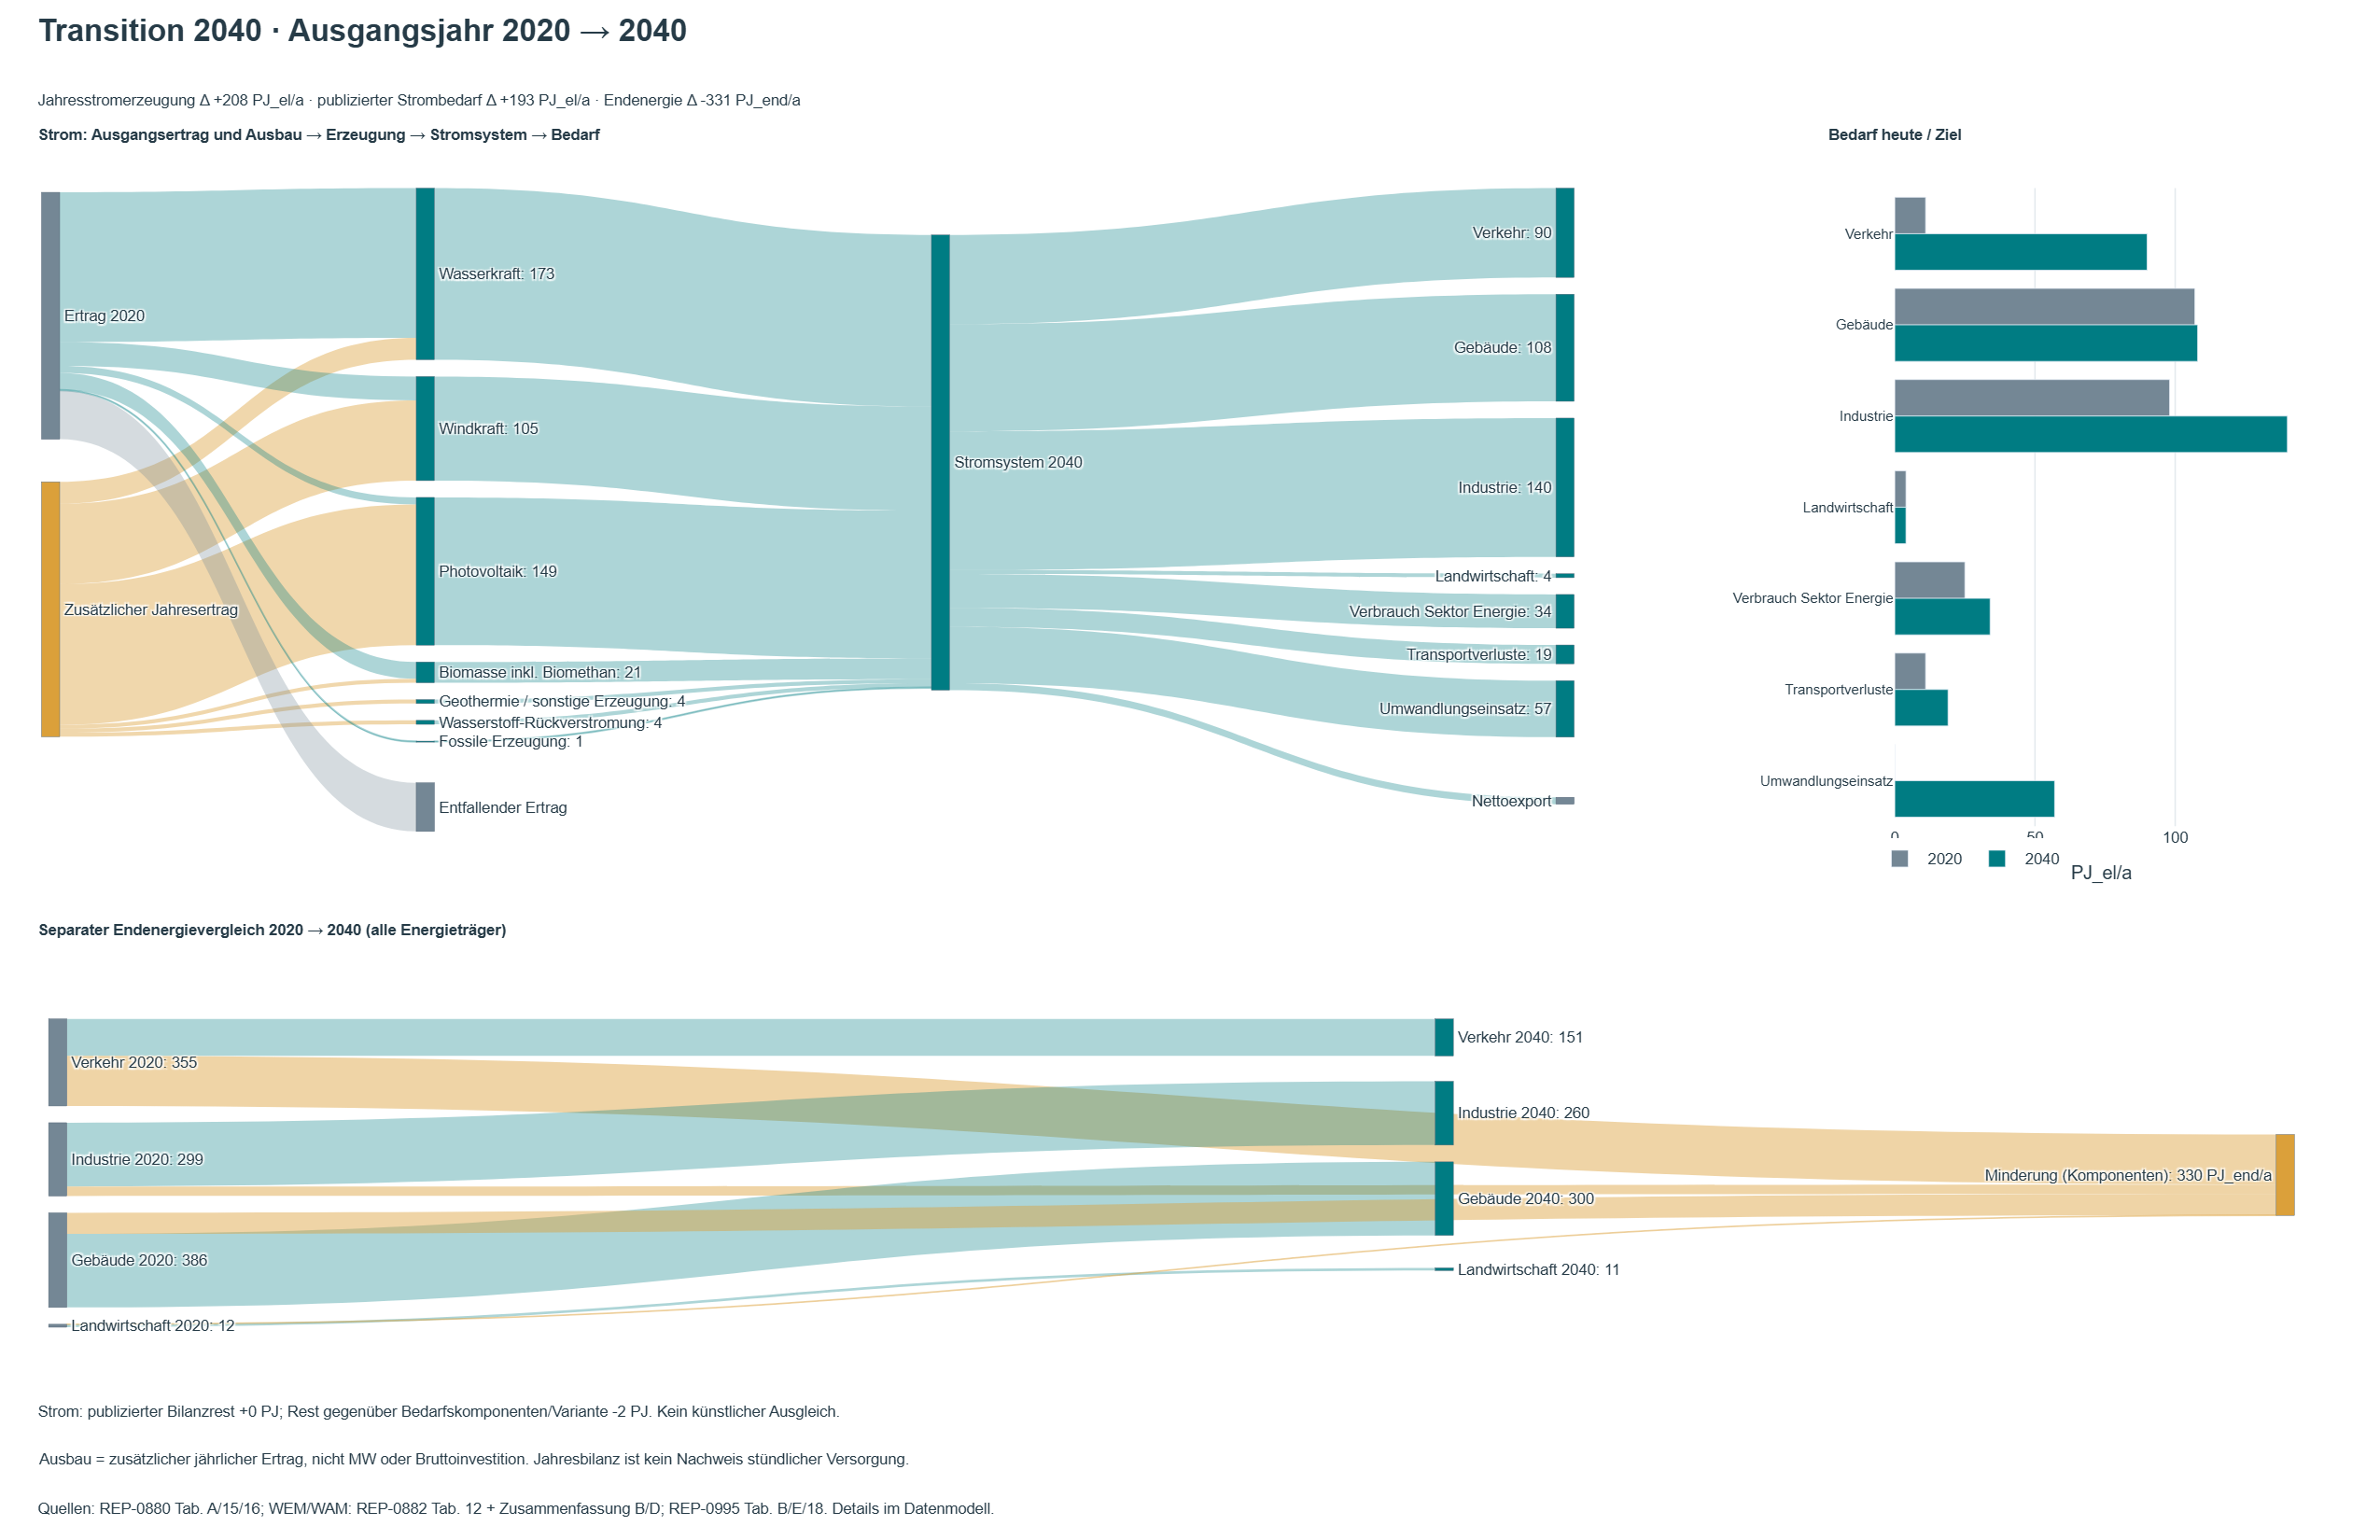
\includegraphics[keepaspectratio]{Kapitel/../Abbildungen/transition_sankey.png}}

}

\caption{\label{fig-transition-sankey}Stromausbau, Strombedarf und
Endenergieminderung gegenüber 2020.}

\end{figure}%

Die Minderung der Endenergie beträgt nach Gesamtsummen 331 PJ/a und nach
gerundeten Sektorkomponenten 330 PJ/a. Für WEM/WAM 2025 folgt die
Normierung Tabelle E in REP-0995; Abweichungen zu Tabelle 19 desselben
Berichts sind im Datenanhang dokumentiert.

\section{Übergang zur Allokation}\label{uxfcbergang-zur-allokation}

Die UBA-Tabellen enthalten weder die für PEQ benötigte Aufteilung der PV
auf Gebäude und Freiflächen noch jene des Verkehrs auf MIV und ÖPNV.
Diese Aufteilungen sind explizite Parameter der Allokation in
Kapitel~\ref{sec-allokation}. Die Quelldaten bleiben davon unverändert.

Die historische Ableitung nach Streicher et al.~bildet den methodischen
Ausgangspunkt; das Referenzszenario dieses Entwurfs ist Transition 2040
(Streicher u.~a. 2010; Schneider u.~a. 2020, 2023).

\chapter{Sektorale Energieallokation}\label{sec-allokation}

Vom nationalen Stromsystem zum Gebäudesektorsaldo und zum
Mobilitätsbudget

Die Allokation verteilt die Stromerzeugung und den Bedarf aus UBA
Transition 2040 auf sektorale Verantwortungsbereiche. Sie liefert zwei
verbundene Größen: den Zielsaldo für Gebäude einschließlich MIV und das
aus zentraler Erzeugung zugeordnete Mobilitätsbudget. Die Rechnung ist
in Anhang~\ref{sec-allokation-notebook} dokumentiert.

\section{Begriffe und
Bilanzgrößen}\label{begriffe-und-bilanzgruxf6uxdfen}

\begin{longtable}[]{@{}
  >{\raggedright\arraybackslash}p{(\linewidth - 2\tabcolsep) * \real{0.5000}}
  >{\raggedright\arraybackslash}p{(\linewidth - 2\tabcolsep) * \real{0.5000}}@{}}
\caption{Glossar der sektoralen
Allokation.}\label{tbl-allokation-glossar}\tabularnewline
\toprule\noalign{}
\begin{minipage}[b]{\linewidth}\raggedright
Begriff
\end{minipage} & \begin{minipage}[b]{\linewidth}\raggedright
Bedeutung im Modell
\end{minipage} \\
\midrule\noalign{}
\endfirsthead
\toprule\noalign{}
\begin{minipage}[b]{\linewidth}\raggedright
Begriff
\end{minipage} & \begin{minipage}[b]{\linewidth}\raggedright
Bedeutung im Modell
\end{minipage} \\
\midrule\noalign{}
\endhead
\bottomrule\noalign{}
\endlastfoot
Zentraler Pool & Für die priorisierten Bedarfe angesetzte
Nicht-PV-Stromerzeugung; „zentral`` bezeichnet die Allokation, nicht
Anlagengröße oder Eigentum. \\
Budgetfähig & Nach der gewählten Zuordnungsregel für diesen Pool
anrechenbar. Der Begriff beschreibt eine Modellentscheidung, keinen
Herkunftsnachweis. \\
Gebäude-PV & Anteil der nationalen PV-Erzeugung, der dem Gebäudesektor
zugeordnet wird. \\
Freiflächen-PV & Im Modell die gesamte PV außerhalb von Gebäuden; sie
bleibt als eigener nationaler Pool ausgewiesen. \\
MIV-Anteil & Anteil des MIV am \textbf{elektrischen Energiebedarf} des
Verkehrs; kein Wege- oder Personenkilometeranteil. \\
ÖPNV & Öffentlicher Personenverkehr; eigene Teilmenge des elektrischen
Verkehrsbedarfs. Übriger Verkehr wird separat geführt. \\
MIV-Budget / Mobilitätsgutschrift & Dem MIV zugeteilte Deckung aus dem
zentralen Pool in PJ Strom/a. Die nutzungsbezogene PE-Gutschrift ist in
Kapitel~\ref{sec-kontext-mobilitaet} definiert. \\
Saldo & Zugeordnete Deckung minus Bedarf; positiv bedeutet Überschuss,
negativ Deckungslücke. \\
\end{longtable}

\section{Erzeugungszuordnung und
Prioritäten}\label{erzeugungszuordnung-und-priorituxe4ten}

Der Referenzfall ordnet die 149 PJ/a PV vollständig den Gebäuden zu.
Freiflächen-PV bleibt in Varianten separat; sie wird nicht in den
zentralen Nicht-PV-Pool umgebucht. Diese Regel macht sichtbar, wie sich
die Gebäudeaufgabe mit der PV-Zuordnung verändert.

Dem zentralen Pool werden Wasserkraft (173 PJ/a), Windkraft (105),
Biomasse (21) und die normierte Position Geothermie/sonstige (4)
zugeordnet: zusammen \textbf{303 PJ/a}. Wasserstoff-Rückverstromung (4
PJ/a) ist im Referenzfall wegen der nicht dokumentierten Herkunft nicht
angerechnet; eine Variante zeigt die vollständige Anrechnung. Fossile
Erzeugung (1 PJ/a) bleibt außerhalb des Pools (Umweltbundesamt 2024,
Tab. 16).

Die zentrale Erzeugung deckt zuerst Industrie, Landwirtschaft,
Energiebranche, Umwandlung, Netzverluste und Nettoexport sowie ÖPNV und
übrigen Verkehr. Bei 20 \% ÖPNV und 80 \% MIV an 90 PJ/a Verkehrsbedarf
verbleiben \textbf{24 PJ/a für MIV}. Die Priorität folgt dem
Allokationsansatz nach Schneider u.~a. (2020) und Schneider u.~a.
(2023); die Mengen stammen aus Transition 2040.

\begin{longtable}[]{@{}
  >{\raggedright\arraybackslash}p{(\linewidth - 2\tabcolsep) * \real{0.5000}}
  >{\raggedright\arraybackslash}p{(\linewidth - 2\tabcolsep) * \real{0.5000}}@{}}
\caption{Zuordnungsregeln des Referenzfalls. Die PV- und Verkehrsanteile
sind Modellannahmen.}\label{tbl-allokation-datenbedarf}\tabularnewline
\toprule\noalign{}
\begin{minipage}[b]{\linewidth}\raggedright
Position
\end{minipage} & \begin{minipage}[b]{\linewidth}\raggedright
Ansatz im Referenzfall
\end{minipage} \\
\midrule\noalign{}
\endfirsthead
\toprule\noalign{}
\begin{minipage}[b]{\linewidth}\raggedright
Position
\end{minipage} & \begin{minipage}[b]{\linewidth}\raggedright
Ansatz im Referenzfall
\end{minipage} \\
\midrule\noalign{}
\endhead
\bottomrule\noalign{}
\endlastfoot
Nicht-PV-Pool & Wasser, Wind, Biomasse, Geothermie/sonstige \\
PV & 100 \% Gebäude, 0 \% Freifläche \\
Verkehr & 80 \% MIV, 20 \% ÖPNV, 0 \% übriger Verkehr \\
Systempositionen & Einmaliger Abzug von Energiebranche, Umwandlung,
Verlusten und Nettoexport \\
H₂-Rückverstromung & 0 \% anrechenbar; Vergleichsvariante mit 100 \% \\
\end{longtable}

\section{Berechnung von Mobilitätsbudget und
Gebäudesaldo}\label{sec-allokation-miv}

Für die Berechnung gelten folgende jährliche Stromgrößen:

{\def\LTcaptype{none} % do not increment counter
\begin{longtable}[]{@{}
  >{\raggedright\arraybackslash}p{(\linewidth - 4\tabcolsep) * \real{0.3333}}
  >{\raggedright\arraybackslash}p{(\linewidth - 4\tabcolsep) * \real{0.3333}}
  >{\raggedright\arraybackslash}p{(\linewidth - 4\tabcolsep) * \real{0.3333}}@{}}
\toprule\noalign{}
\begin{minipage}[b]{\linewidth}\raggedright
Symbol
\end{minipage} & \begin{minipage}[b]{\linewidth}\raggedright
Definition
\end{minipage} & \begin{minipage}[b]{\linewidth}\raggedright
Einheit
\end{minipage} \\
\midrule\noalign{}
\endhead
\bottomrule\noalign{}
\endlastfoot
\(E_{\mathrm{Z}}\) & Angerechnete zentrale Erzeugung & PJ/a \\
\(E_{\mathrm{V}}\) & Summe der priorisierten Bedarfe einschließlich
ÖPNV, übrigen Verkehrs und Nettoexports & PJ/a \\
\(E_{\mathrm{MIV}}\) & Elektrischer MIV-Bedarf & PJ/a \\
\(G_{\mathrm{MIV}}\) & Zugeordnetes MIV-Budget & PJ/a \\
\(E_{\mathrm{PV,Geb}}\) & Dem Gebäude zugeordnete PV-Erzeugung & PJ/a \\
\(E_{\mathrm{Geb}}\) & Betriebsstrombedarf des Gebäudesektors & PJ/a \\
\(B_{\mathrm{Geb,Ziel}}\) & Zielsaldo für Gebäude einschließlich MIV &
PJ/a \\
\end{longtable}
}

Das Budget ist auf den verfügbaren positiven Rest und den MIV-Bedarf
begrenzt:

\begin{equation}\protect\phantomsection\label{eq-miv-restbudget}{
G_{\mathrm{MIV}}=\min\left(E_{\mathrm{MIV}},\max(0,E_{\mathrm{Z}}-E_{\mathrm{V}})\right).
}\end{equation}

Ein negativer Rest \(E_{\mathrm{Z}}-E_{\mathrm{V}}\) wird als zentrale
Unterdeckung ausgewiesen. Ein Rest oberhalb des MIV-Bedarfs bleibt
unverteilt.

\begin{equation}\protect\phantomsection\label{eq-gebaeudesektor-zielsaldo}{
B_{\mathrm{Geb,Ziel}}=E_{\mathrm{PV,Geb}}+G_{\mathrm{MIV}}-E_{\mathrm{Geb}}-E_{\mathrm{MIV}}.
}\end{equation}

Im Referenzfall: \(149+24-108-72=-7\) PJ/a. Ohne MIV beträgt der
Gebäudesaldo \(149-108=+41\) PJ/a. Das MIV-Budget von 24 PJ/a entspricht
6,667 TWh/a.

\section{Quantitative Allokation und
Stellschrauben}\label{sec-allokation-ergebnisse}

Die Rechnung verwendet 457 PJ/a Erzeugung, 7 PJ/a Nettoexport und 452
PJ/a Bedarfskomponenten. Der Rest von −2 PJ/a bleibt in der nationalen
Zuordnungsbilanz erhalten. Die veröffentlichten Summen und ihre
Rundungsreste stehen in Anhang~\ref{sec-szenariotabellen}.

Die folgenden Tabellen zeigen \textbf{Gesamtmenge und Teilmengen}. Alle
Werte sind PJ Strom/a. PV-Anteile beziehen sich auf die nationale
PV-Erzeugung; Verkehrsanteile auf den nationalen elektrischen
Verkehrsbedarf. Die gewählten Anteile sind Varianten des Modells, keine
von UBA veröffentlichten Aufteilungen.

\begin{longtable}[]{@{}
  >{\raggedright\arraybackslash}p{(\linewidth - 8\tabcolsep) * \real{0.2000}}
  >{\raggedright\arraybackslash}p{(\linewidth - 8\tabcolsep) * \real{0.2000}}
  >{\raggedright\arraybackslash}p{(\linewidth - 8\tabcolsep) * \real{0.2000}}
  >{\raggedright\arraybackslash}p{(\linewidth - 8\tabcolsep) * \real{0.2000}}
  >{\raggedright\arraybackslash}p{(\linewidth - 8\tabcolsep) * \real{0.2000}}@{}}
\caption{PV-Aufteilung in PJ Strom/a; Freiflächenanteil bezogen auf die
gesamte PV-Erzeugung.}\label{tbl-allokation-pv}\tabularnewline
\toprule\noalign{}
\begin{minipage}[b]{\linewidth}\raggedright
Variante
\end{minipage} & \begin{minipage}[b]{\linewidth}\raggedright
PV gesamt
\end{minipage} & \begin{minipage}[b]{\linewidth}\raggedright
PV Gebäude
\end{minipage} & \begin{minipage}[b]{\linewidth}\raggedright
PV Freifläche
\end{minipage} & \begin{minipage}[b]{\linewidth}\raggedright
Freiflächen-Anteil {[}\%{]}
\end{minipage} \\
\midrule\noalign{}
\endfirsthead
\toprule\noalign{}
\begin{minipage}[b]{\linewidth}\raggedright
Variante
\end{minipage} & \begin{minipage}[b]{\linewidth}\raggedright
PV gesamt
\end{minipage} & \begin{minipage}[b]{\linewidth}\raggedright
PV Gebäude
\end{minipage} & \begin{minipage}[b]{\linewidth}\raggedright
PV Freifläche
\end{minipage} & \begin{minipage}[b]{\linewidth}\raggedright
Freiflächen-Anteil {[}\%{]}
\end{minipage} \\
\midrule\noalign{}
\endhead
\bottomrule\noalign{}
\endlastfoot
Referenz & 149 & 149.0 & 0.0 & 0.0 \\
20 \% Freiflächen-PV & 149 & 119.2 & 29.8 & 20.0 \\
60 \% MIV & 149 & 149.0 & 0.0 & 0.0 \\
40 \% MIV: Konflikt & 149 & 149.0 & 0.0 & 0.0 \\
H₂ vollständig angerechnet & 149 & 149.0 & 0.0 & 0.0 \\
\end{longtable}

\begin{longtable}[]{@{}
  >{\raggedright\arraybackslash}p{(\linewidth - 10\tabcolsep) * \real{0.1667}}
  >{\raggedright\arraybackslash}p{(\linewidth - 10\tabcolsep) * \real{0.1667}}
  >{\raggedright\arraybackslash}p{(\linewidth - 10\tabcolsep) * \real{0.1667}}
  >{\raggedright\arraybackslash}p{(\linewidth - 10\tabcolsep) * \real{0.1667}}
  >{\raggedright\arraybackslash}p{(\linewidth - 10\tabcolsep) * \real{0.1667}}
  >{\raggedright\arraybackslash}p{(\linewidth - 10\tabcolsep) * \real{0.1667}}@{}}
\caption{Verkehrsaufteilung in PJ Strom/a; MIV-Anteil bezogen auf den
elektrischen
Verkehrsbedarf.}\label{tbl-allokation-verkehr}\tabularnewline
\toprule\noalign{}
\begin{minipage}[b]{\linewidth}\raggedright
Variante
\end{minipage} & \begin{minipage}[b]{\linewidth}\raggedright
Verkehr gesamt
\end{minipage} & \begin{minipage}[b]{\linewidth}\raggedright
ÖPNV
\end{minipage} & \begin{minipage}[b]{\linewidth}\raggedright
MIV
\end{minipage} & \begin{minipage}[b]{\linewidth}\raggedright
Übriger Verkehr
\end{minipage} & \begin{minipage}[b]{\linewidth}\raggedright
MIV-Anteil {[}\%{]}
\end{minipage} \\
\midrule\noalign{}
\endfirsthead
\toprule\noalign{}
\begin{minipage}[b]{\linewidth}\raggedright
Variante
\end{minipage} & \begin{minipage}[b]{\linewidth}\raggedright
Verkehr gesamt
\end{minipage} & \begin{minipage}[b]{\linewidth}\raggedright
ÖPNV
\end{minipage} & \begin{minipage}[b]{\linewidth}\raggedright
MIV
\end{minipage} & \begin{minipage}[b]{\linewidth}\raggedright
Übriger Verkehr
\end{minipage} & \begin{minipage}[b]{\linewidth}\raggedright
MIV-Anteil {[}\%{]}
\end{minipage} \\
\midrule\noalign{}
\endhead
\bottomrule\noalign{}
\endlastfoot
Referenz & 90 & 18.0 & 72.0 & 0 & 80.0 \\
20 \% Freiflächen-PV & 90 & 18.0 & 72.0 & 0 & 80.0 \\
60 \% MIV & 90 & 36.0 & 54.0 & 0 & 60.0 \\
40 \% MIV: Konflikt & 90 & 54.0 & 36.0 & 0 & 40.0 \\
H₂ vollständig angerechnet & 90 & 18.0 & 72.0 & 0 & 80.0 \\
\end{longtable}

\begin{longtable}[]{@{}
  >{\raggedright\arraybackslash}p{(\linewidth - 10\tabcolsep) * \real{0.1667}}
  >{\raggedright\arraybackslash}p{(\linewidth - 10\tabcolsep) * \real{0.1667}}
  >{\raggedright\arraybackslash}p{(\linewidth - 10\tabcolsep) * \real{0.1667}}
  >{\raggedright\arraybackslash}p{(\linewidth - 10\tabcolsep) * \real{0.1667}}
  >{\raggedright\arraybackslash}p{(\linewidth - 10\tabcolsep) * \real{0.1667}}
  >{\raggedright\arraybackslash}p{(\linewidth - 10\tabcolsep) * \real{0.1667}}@{}}
\caption{Allokationsergebnisse in PJ Strom/a. Negativer zentraler Rest
kennzeichnet ungedeckte
Vorrangbedarfe.}\label{tbl-allokation-vorlaeufig}\tabularnewline
\toprule\noalign{}
\begin{minipage}[b]{\linewidth}\raggedright
Variante
\end{minipage} & \begin{minipage}[b]{\linewidth}\raggedright
H₂-Anrechnung {[}\%{]}
\end{minipage} & \begin{minipage}[b]{\linewidth}\raggedright
MIV-Budget
\end{minipage} & \begin{minipage}[b]{\linewidth}\raggedright
Saldo
\end{minipage} & \begin{minipage}[b]{\linewidth}\raggedright
Zentraler Rest
\end{minipage} & \begin{minipage}[b]{\linewidth}\raggedright
Vorrang gedeckt
\end{minipage} \\
\midrule\noalign{}
\endfirsthead
\toprule\noalign{}
\begin{minipage}[b]{\linewidth}\raggedright
Variante
\end{minipage} & \begin{minipage}[b]{\linewidth}\raggedright
H₂-Anrechnung {[}\%{]}
\end{minipage} & \begin{minipage}[b]{\linewidth}\raggedright
MIV-Budget
\end{minipage} & \begin{minipage}[b]{\linewidth}\raggedright
Saldo
\end{minipage} & \begin{minipage}[b]{\linewidth}\raggedright
Zentraler Rest
\end{minipage} & \begin{minipage}[b]{\linewidth}\raggedright
Vorrang gedeckt
\end{minipage} \\
\midrule\noalign{}
\endhead
\bottomrule\noalign{}
\endlastfoot
Referenz & 0 & 24.0 & -7.0 & 0.0 & ja \\
20 \% Freiflächen-PV & 0 & 24.0 & -36.8 & 0.0 & ja \\
60 \% MIV & 0 & 6.0 & -7.0 & 0.0 & ja \\
40 \% MIV: Konflikt & 0 & 0.0 & 5.0 & -12.0 & nein \\
H₂ vollständig angerechnet & 100 & 28.0 & -3.0 & 0.0 & ja \\
\end{longtable}

Je Variante stehen \textbf{Gebäudestrombedarf + MIV-Strombedarf} der
Deckung aus \textbf{Gebäude-PV + Mobilitätsgutschrift} gegenüber. Das
zweite Diagramm zeigt den resultierenden Saldo und einen etwaigen
zentralen Fehlbetrag. Der positive Gebäudesaldo der 40-\%-MIV-Variante
ist daher zusammen mit der zentralen Unterdeckung von 12 PJ/a zu lesen.

Mit \(f\) als Freiflächenanteil der PV, \(m\) als MIV-Anteil am Verkehr
und \(h\) als angerechnetem Anteil der H₂-Rückverstromung ergibt sich
bei gedeckter Priorität und nicht bindender Budgetobergrenze:

\[G_{\mathrm{MIV}}=90m-48+4h,\qquad B_{\mathrm{Geb,Ziel}}=-7+4h-149f.\]

Eine Änderung des MIV-Anteils verändert Bedarf und Budget im selben
Umfang, solange diese Bedingungen gelten. Mehr Freiflächen-PV vermindert
dagegen die dem Gebäude zugeordnete Deckung. Die nicht zugeordnete PV
bleibt Bestandteil der nationalen Bilanz.

\section{Übergang zur Gebäude- und
Quartiersbewertung}\label{uxfcbergang-zur-gebuxe4ude--und-quartiersbewertung}

Der Gebäudepool erreicht −59,25 PJ/a im Betrieb und −107,25 PJ/a
einschließlich derselben MIV-Zuordnung. Der Abstand zum Top-down-Ziel
beträgt damit −100,25 PJ/a (Kapitel~\ref{sec-gebaeudebestand}). Er
kennzeichnet Unterschiede in PV-Erzeugung und Gebäudebedarf der beiden
Szenarien.

Die sektorale Kalibrierung erfolgt auf elektrischer Endenergiebasis. Für
den Quartiersnachweis werden die Ergebnisse mit dem dokumentierten
heutigen PE-Faktorensatz bewertet. Die nutzungsbezogene Verteilung des
Mobilitätsbudgets steht in Kapitel~\ref{sec-kontext-mobilitaet}, die
Dichte- und Typologiekalibrierung in Kapitel~\ref{sec-kalibrierung}. Der
Entwurf dokumentiert die verwendeten Annahmen und ihren Ergebnisstand;
eine normative Festlegung von PEQ-Flächenanteilen und neuer
Dichtefunktion ist darin nicht enthalten.

\chapter{Gebäudebestand und Entwicklungsszenario
2040}\label{sec-gebaeudebestand}

Gebäudetypologien, nationale Flächen und GFZ-Verteilungen als
Bottom-up-Grundlage der PEQ-Kalibrierung

Das Gebäudesektormodell verknüpft die Flächenstruktur des Zieljahres
2040 mit den energetischen Kennwerten der Gebäudetypen und ihren
Dichteverteilungen. Es bildet die Bottom-up-Seite zur sektoralen
Allokation in Kapitel~\ref{sec-allokation}. Die Auswertung des Pools
ergibt \textbf{137,49 PJ/a Strombedarf}, \textbf{78,25 PJ/a
PV-Erzeugung} und einen \textbf{betrieblichen Stromsaldo von −59,25
PJ/a}. Diese Zahlen beschreiben den gelieferten Szenariostand. Der
Abgleich mit UBA Transition zeigt den Szenarioabstand.

Die vollständige Herleitung, Eingabetabellen, Formeln und
Bilanzprüfungen stehen im ausführbaren Anhang
Anhang~\ref{sec-gebaeudesektormodell}. Die Berechnungen sind unmittelbar
in dessen Notebook-Zellen enthalten.

\section{Datenbasis, Flächenbegriffe und
Bezugsjahre}\label{datenbasis-fluxe4chenbegriffe-und-bezugsjahre}

Grundlage ist \texttt{Building-Sector\_Pool\ 1.xlsx}, einschließlich der
am 23.10.2026 ergänzten GFZ-Anteile. Das Blatt \texttt{Strombed\_estim}
enthält die maßgeblichen Flächen- und Energiekennwerte,
\texttt{zuordnung\_gfz} die Zuordnung nach Nutzung und Geschoßklasse.
Das Simulationsblatt \texttt{Tabelle2} liefert Einheiten und ergänzende
Anwendungen. Alle 900 Archetypenschlüssel sind eindeutig und lassen sich
vollständig mit den Simulationsergebnissen verbinden. Die gespeicherten
Kennwerte stimmen mit den im Kennwertblatt referenzierten
Simulationswerten überein; eine erneute PEExcel-Simulation ist damit
nicht verbunden.

Die nationale Flächensumme beträgt \textbf{1.126,579 Mio. m² BGF für
2040}, gegenüber \textbf{1.112,341 Mio. m² BGF} in der Quellspalte
„heute``. Deren konkretes Bezugsjahr ist nicht bestätigt. Sie wird
deshalb nicht mit 2020 gleichgesetzt. Die Energiekennwerte beziehen sich
laut Simulationsblatt auf \textbf{NGF}. Für die Aggregation gilt die aus
der bestehenden GFZ-Analyse übernommene einheitliche Modellannahme:

\[
A_{NGF,k,y}=0{,}8\,A_{BGF,k,y}.
\]

Für 2040 folgen daraus 901,263 Mio. m² NGF. Der Flächenfaktor ist für
alle Typen einheitlich. Es erfolgt keine Skalierung auf die
GFZ-Bestandsfläche von 1.058,935 Mio. m² BGF oder auf die separate
Flächenannahme der THG-Allokation. Diese Größen haben unterschiedliche
Grundlagen.

Das ältere Blatt \texttt{reduced} enthält 696,615 Mio. m² NGF, 486
positiv gewichtete Varianten, 264 echte Nullwerte und 6.450 leere
Flächenfelder. Im neuen Kennwertblatt sind 603 Typen für 2040 positiv
gewichtet und 297 explizit null; Flächenwerte fehlen dort nicht. Die
unterschiedlichen Flächenbezüge, Variantenabdeckungen und Summen werden
in Kapitel~\ref{sec-gebaeude-flaechen} verglichen. Der ältere Datensatz
wird nicht als additive Fläche oder Ersatzgewichtung verwendet.
\texttt{save} ist ein zusätzlicher Projekt-/Presetstand und keine
nationale Flächenbilanz.

\section{Energetische Gebäudetypologien
2040}\label{sec-gebaeudetypologien}

Der vollständige Typenschlüssel kombiniert \textbf{Geometrie, Baualter
beziehungsweise Hüllstandard, Wärmeversorgung, PV-Ausstattung und
Flexibilität}. Die zehn Geometrieklassen sind daher nicht mit zehn
energetischen Klassen gleichzusetzen. Der ausgewertete Bestand umfasst
neun Baualters-/Hüllcodes und zehn Wärmeversorgungsvarianten. Alle 900
simulierten Typen tragen die Variante \texttt{PV30\textbar{}noFlex}; die
übrigen PV-/Flexibilitätsvarianten des 7.200 Szenarien umfassenden
Gesamtpools erhalten keine ungeprüft übertragenen Kennwerte.

\texttt{Neu\_10cm}, \texttt{Neu\_20cm} und \texttt{Neu\_30cm} bezeichnen
Hüllcodes. Die Zugehörigkeit zu Bestand, Neubau oder Sanierung folgt den
separat gelieferten Anteilen, nicht allein dem Wort „Neu``. Das Feld
„Energetischer Standard`` ist noch leer. Auch eine PEQ-Presetbezeichnung
oder ein positiver Stromsaldo belegt für sich keine PEQ-Konformität.

\begin{longtable}[]{@{}
  >{\raggedright\arraybackslash}p{(\linewidth - 8\tabcolsep) * \real{0.2000}}
  >{\raggedright\arraybackslash}p{(\linewidth - 8\tabcolsep) * \real{0.2000}}
  >{\raggedright\arraybackslash}p{(\linewidth - 8\tabcolsep) * \real{0.2000}}
  >{\raggedright\arraybackslash}p{(\linewidth - 8\tabcolsep) * \real{0.2000}}
  >{\raggedright\arraybackslash}p{(\linewidth - 8\tabcolsep) * \real{0.2000}}@{}}
\caption{Gelieferte Flächen und BGF-gewichtete Dichte-Erwartungswerte.
Heute: Bezugsjahr offen; Dichtefunktion in elektrischer
Energie.}\label{tbl-gebaeude-typologien}\tabularnewline
\toprule\noalign{}
\begin{minipage}[b]{\linewidth}\raggedright
Geometrie
\end{minipage} & \begin{minipage}[b]{\linewidth}\raggedright
BGF heute {[}Mio. m²{]}
\end{minipage} & \begin{minipage}[b]{\linewidth}\raggedright
BGF 2040 {[}Mio. m²{]}
\end{minipage} & \begin{minipage}[b]{\linewidth}\raggedright
GFZ\_Mittel
\end{minipage} & \begin{minipage}[b]{\linewidth}\raggedright
c\_D\_EE\_BGF
\end{minipage} \\
\midrule\noalign{}
\endfirsthead
\toprule\noalign{}
\begin{minipage}[b]{\linewidth}\raggedright
Geometrie
\end{minipage} & \begin{minipage}[b]{\linewidth}\raggedright
BGF heute {[}Mio. m²{]}
\end{minipage} & \begin{minipage}[b]{\linewidth}\raggedright
BGF 2040 {[}Mio. m²{]}
\end{minipage} & \begin{minipage}[b]{\linewidth}\raggedright
GFZ\_Mittel
\end{minipage} & \begin{minipage}[b]{\linewidth}\raggedright
c\_D\_EE\_BGF
\end{minipage} \\
\midrule\noalign{}
\endhead
\bottomrule\noalign{}
\endlastfoot
EFH\_1G & 129,675 & 131,047 & 0,318 & -41,631 \\
EFH\_2G & 186,891 & 189,492 & 0,615 & -22,798 \\
GWB\_5G & 39,452 & 39,941 & 2,266 & 8,966 \\
GWB\_7G & 81,032 & 82,108 & 4,000 & 16,440 \\
MFH\_2G & 0,000 & 0,000 & offen & offen \\
MFH\_4G & 65,007 & 65,865 & 1,541 & 1,432 \\
NiWo\_1G & 90,878 & 92,026 & 0,491 & -29,353 \\
NiWo\_2G & 138,179 & 139,840 & 0,875 & -13,124 \\
NiWo\_3G & 194,334 & 196,767 & 2,183 & 3,924 \\
RH\_2G & 186,891 & 189,492 & 0,615 & -22,798 \\
\end{longtable}

Die Geometrie MFH\_2G besitzt derzeit keine positive nationale Fläche.
Ihre fehlende GFZ-Zuordnung bleibt sichtbar; für sie wird kein
Dichte-Erwartungswert erfunden. Für alle positiv gewichteten Typen liegt
eine Zuordnung vor.

\section{Flächenentwicklung vom Bestand zum
Zieljahr}\label{fluxe4chenentwicklung-vom-bestand-zum-zieljahr}

Die gelieferte Gesamtfläche steigt zwischen „heute`` und 2040 um rund
14,238 Mio. m² BGF beziehungsweise 1,28 \%. Die Spalten Bestand, Neubau
und Sanierung enthalten innerhalb der Archetypen Anteile, die auf jeder
positiv gewichteten 2040-Fläche zusammen eins ergeben. Flächengewichtet
resultiert:

\begin{longtable}[]{@{}ll@{}}
\caption{Flächengewichtete Zuordnung zu Bestand, Neubau und Sanierung im
Zieljahr.}\label{tbl-gebaeude-status}\tabularnewline
\toprule\noalign{}
Zustand & BGF 2040 {[}Mio. m²{]} \\
\midrule\noalign{}
\endfirsthead
\toprule\noalign{}
Zustand & BGF 2040 {[}Mio. m²{]} \\
\midrule\noalign{}
\endhead
\bottomrule\noalign{}
\endlastfoot
Bestand & 779,528 \\
Neubau & 320,354 \\
Sanierung & 26,696 \\
\end{longtable}

\begin{figure}

\centering{

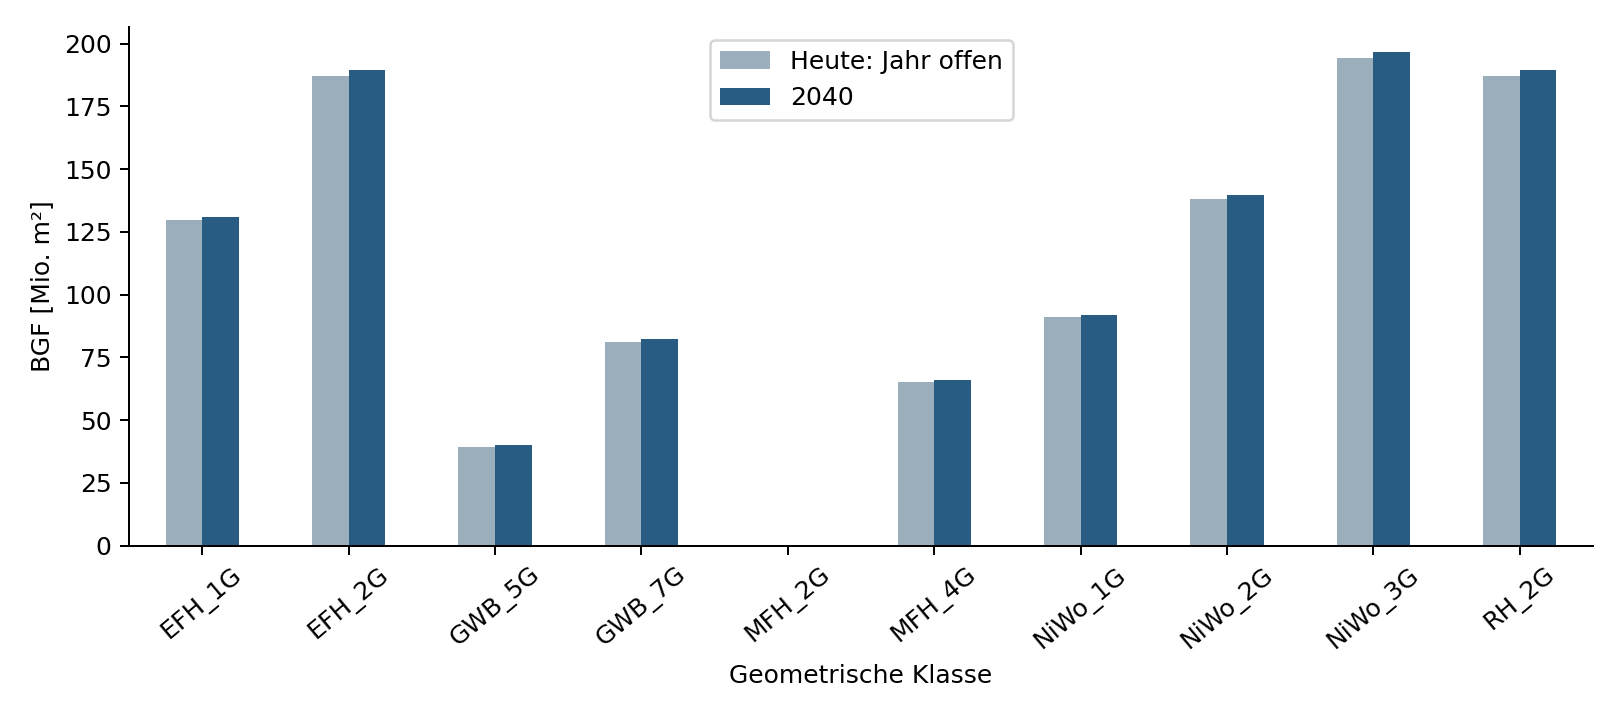
\includegraphics[width=1\linewidth,height=\textheight,keepaspectratio]{Kapitel/../Berechnungen/gebaeudesektormodell/outputs/flaechen.png}

}

\caption{\label{fig-gebaeude-flaechen}Flächenverteilung nach Geometrie.
„Heute`` bezeichnet die gleichnamige Quellspalte mit nicht festgelegtem
Bezugsjahr.}

\end{figure}%

Die Neubaufläche ist nicht mit dem Nettoflächenzuwachs gleichzusetzen.
Für einen nachvollziehbaren Entwicklungspfad fehlen die zeitliche
Definition dieser Kategorien und eine Übergangsbilanz mit Abbruch,
Ersatzneubau und Sanierung. Die Reinschrift enthält ein separates,
leeres Feld für BGF 2020. Es wird nicht automatisch aus „heute``
gefüllt.

\section{Energetische Performance, Strombedarf und
PV}\label{energetische-performance-strombedarf-und-pv}

Die PV-Erzeugung wird \textbf{aus der Typen-Excel übernommen}:
\texttt{PV\_total\_direct} plus \texttt{PV\_to\_Egrid} in
\texttt{Strombed\_estim}, gegengeprüft gegen \texttt{PV\_total} in
\texttt{Tabelle2}. Das Sektormodell simuliert keine eigenen PV-Flächen
oder Erträge. Alle gelieferten Typen verwenden die Variante
\texttt{PV30\textbar{}noFlex}. Die nationale Erzeugung entsteht durch
Multiplikation des spezifischen Ertrags mit der zugeordneten NGF; eine
zusätzliche GFZ-bedingte Skalierung der PV findet nicht statt.

Netzbezug und Bruttostrombedarf werden konsequent getrennt. Für die
vorliegenden Varianten ohne Speicher, Flexibilität oder simulierte
Mobilität gilt:

\[
E_{el}=E_{Netzbezug}+E_{PV,direkt},\qquad E_{PV}=E_{PV,direkt}+E_{PV,Export}.
\]

Der physische Stromsaldo ist sowohl als PV-Erzeugung minus Strombedarf
als auch als PV-Netzeinspeisung minus Netzbezug bestimmbar. Beide Wege
stimmen in der Typenprüfung überein. PV-Direktverbrauch wird nicht
doppelt als Deckung angesetzt.

\begin{longtable}[]{@{}llll@{}}
\caption{Strombilanz 2040 aus den gelieferten Typenkennwerten bei
NGF/BGF = 0.8.}\label{tbl-gebaeude-strom}\tabularnewline
\toprule\noalign{}
Größe & kWh/(m² NGF a) & GWh/a & PJ/a \\
\midrule\noalign{}
\endfirsthead
\toprule\noalign{}
Größe & kWh/(m² NGF a) & GWh/a & PJ/a \\
\midrule\noalign{}
\endhead
\bottomrule\noalign{}
\endlastfoot
Strombedarf & 42,377 & 38.192,572 & 137,493 \\
PV\_Erzeugung & 24,116 & 21.734,851 & 78,245 \\
Grid\_to\_building\_min & 34,899 & 31.452,734 & 113,230 \\
PV\_total\_direct & 7,478 & 6.739,839 & 24,263 \\
PV\_to\_Egrid & 16,638 & 14.995,012 & 53,982 \\
Stromsaldo & -18,261 & -16.457,722 & -59,248 \\
\end{longtable}

\begin{figure}

\centering{

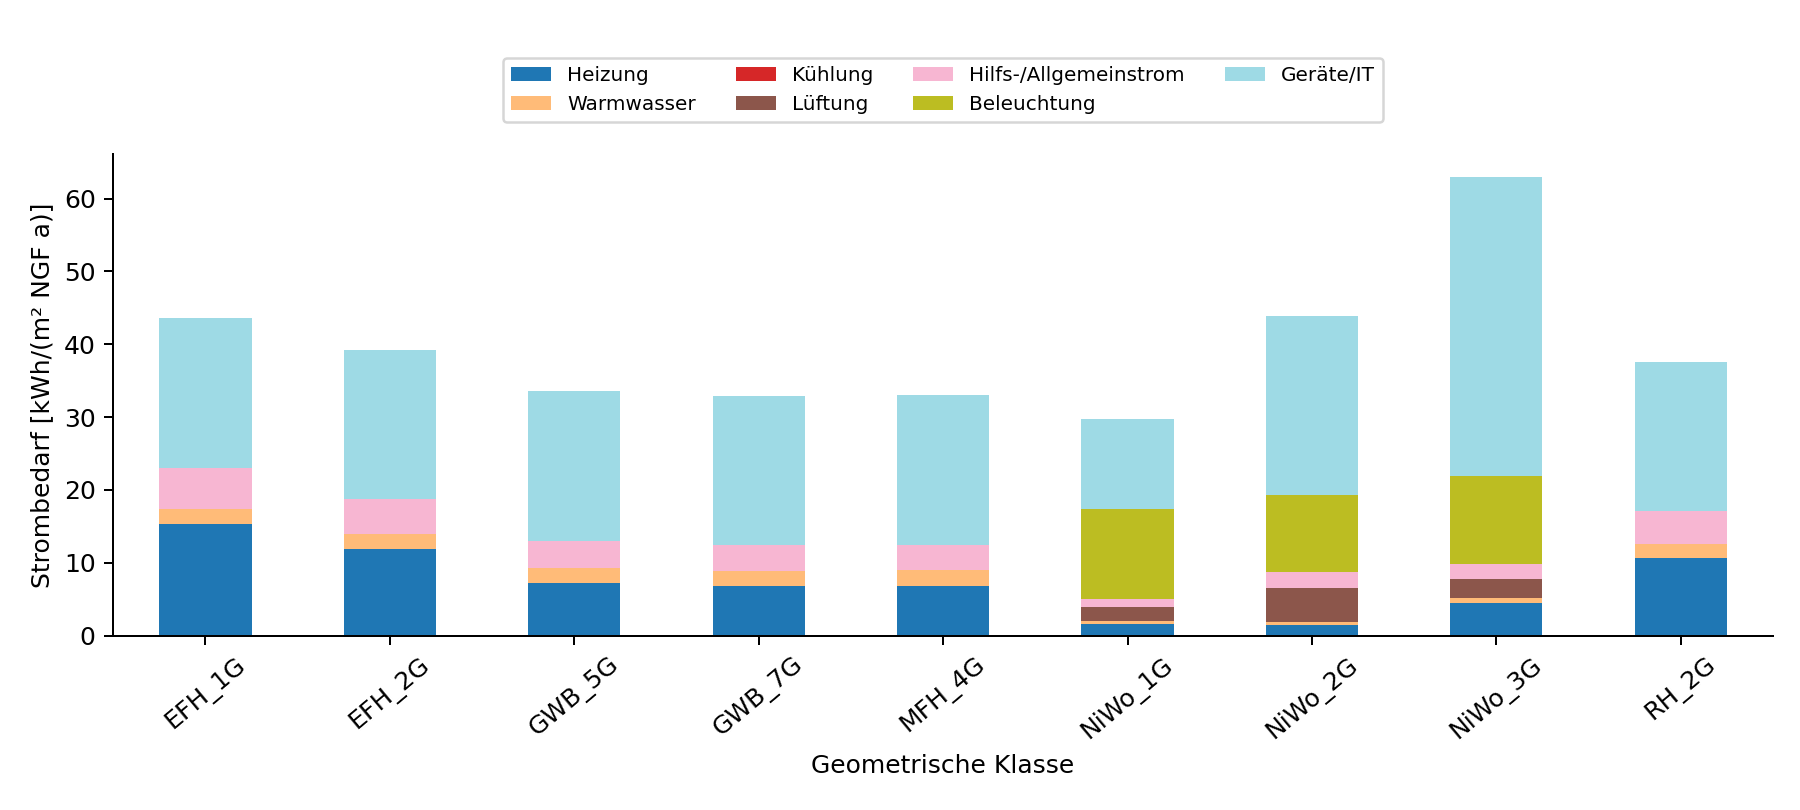
\includegraphics[width=1\linewidth,height=\textheight,keepaspectratio]{Kapitel/../Berechnungen/gebaeudesektormodell/outputs/strom_anwendungen.png}

}

\caption{\label{fig-gebaeude-strom-anwendungen}Flächengewichteter
spezifischer Strombedarf nach Anwendungen. Hilfsstrom wird aus den
Heiz-/Warmwassersummen herausgelöst und gemeinsam mit Allgemeinstrom
dargestellt.}

\end{figure}%

Die Kennwerte unterscheiden Heizung, Warmwasser, Kühlung, Lüftung,
Hilfs-/Allgemeinstrom, Beleuchtung und Geräte/IT. Kühlung ist im
gelieferten Simulationsstand null. Das ist eine Eigenschaft dieser
Simulationen und keine Bestätigung, dass im nationalen Gebäudesektor
2040 kein Kühlbedarf besteht. Die detaillierte Herleitung steht in
Kapitel~\ref{sec-gebaeude-strom}.

\section{Endenergie und
Primärenergie}\label{endenergie-und-primuxe4renergie}

Fernwärme-, Gas-, Biomasse- und Ölbedarfe werden eigenständig
bilanziert. Die Sammelgröße \texttt{EUI\_other} wird bei den als
\texttt{Oel} gekennzeichneten Typen Öl zugeordnet; weitere Beträge
blieben separat unter sonstiger thermischer Endenergie erhalten.

\begin{longtable}[]{@{}llll@{}}
\caption{Endenergie 2040 nach Energieträgern. Strom enthält
PV-Direktverbrauch; sonstige thermische Energie wird separat
geführt.}\label{tbl-gebaeude-endenergie}\tabularnewline
\toprule\noalign{}
Träger & kWh/(m² NGF a) & GWh/a & PJ/a \\
\midrule\noalign{}
\endfirsthead
\toprule\noalign{}
Träger & kWh/(m² NGF a) & GWh/a & PJ/a \\
\midrule\noalign{}
\endhead
\bottomrule\noalign{}
\endlastfoot
Strom (Bruttobedarf) & 42,377 & 38.192,572 & 137,493 \\
Fernwärme & 31,499 & 28.388,612 & 102,199 \\
Gas & 23,631 & 21.297,969 & 76,673 \\
Biomasse & 21,346 & 19.238,623 & 69,259 \\
Öl & 18,034 & 16.253,386 & 58,512 \\
Sonstige thermisch & 0,000 & 0,000 & 0,000 \\
\end{longtable}

\begin{figure}

\centering{

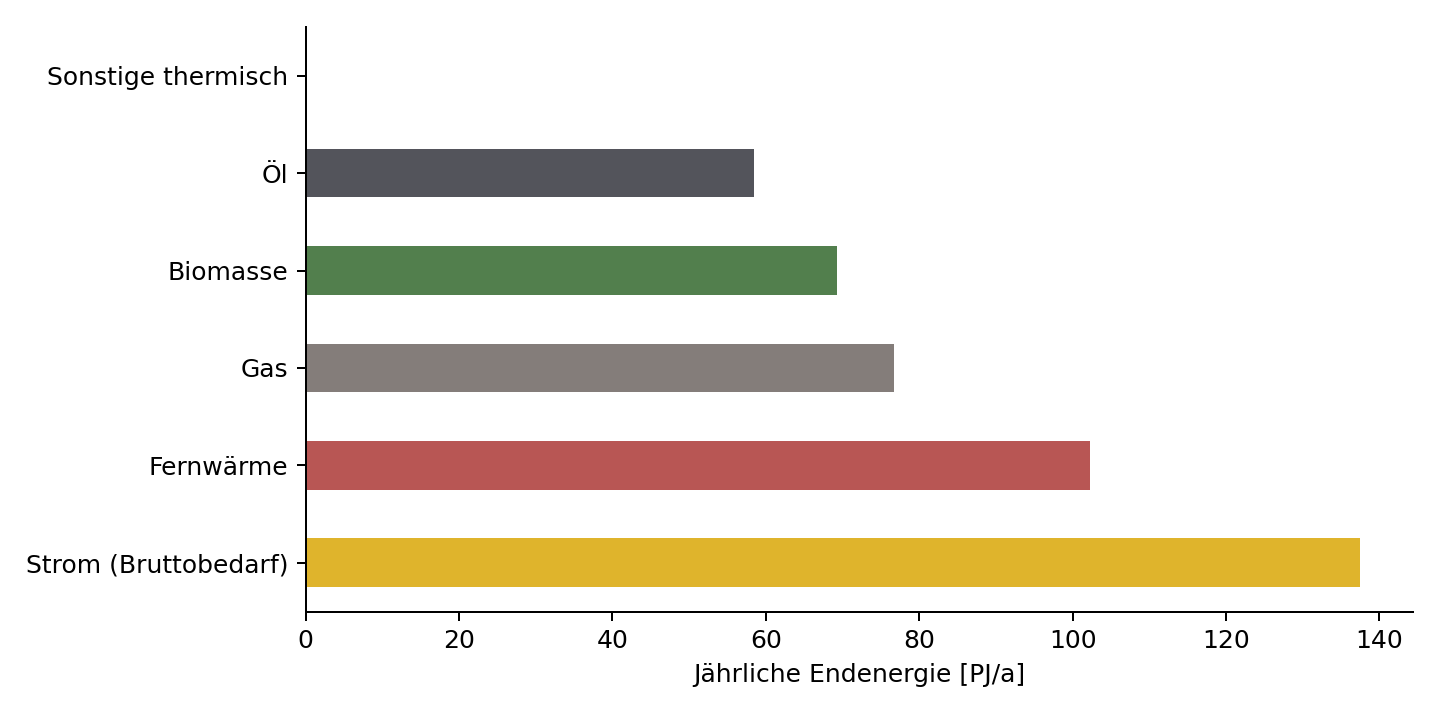
\includegraphics[width=1\linewidth,height=\textheight,keepaspectratio]{Kapitel/../Berechnungen/gebaeudesektormodell/outputs/endenergie.png}

}

\caption{\label{fig-gebaeude-endenergie}Endenergie des gelieferten
2040-Pools nach Energieträgern.}

\end{figure}%

Insbesondere die verbleibenden \textbf{76,67 PJ/a Gas} und \textbf{58,51
PJ/a Öl} zeigen, dass die gelieferte Flächen-/Versorgungsstruktur kein
vollständig dekarbonisiertes Szenario darstellt. Diese Mengen werden
weder als Strom behandelt noch aus der Bilanz entfernt. Die
Anwendungsaufteilung der thermischen Energie steht in
Kapitel~\ref{sec-gebaeude-endenergie}.

Die Primärenergiebilanz aggregiert die gelieferten Import- und
Exportkennwerte. Sie enthält keine virtuellen Dichte-, Mobilitäts- oder
Sanierungsgutschriften:

\begin{longtable}[]{@{}lll@{}}
\caption{Gelieferter PE-Bewertungsstand; Faktorversion und Bezugsjahr
noch zu bestätigen, ohne virtuelle
Kontextwerte.}\label{tbl-gebaeude-pe}\tabularnewline
\toprule\noalign{}
Größe & GWh\_PE/a & PJ\_PE/a \\
\midrule\noalign{}
\endfirsthead
\toprule\noalign{}
Größe & GWh\_PE/a & PJ\_PE/a \\
\midrule\noalign{}
\endhead
\bottomrule\noalign{}
\endlastfoot
PEI\_grid\_import & 59.495,871 & 214,185 \\
PEI\_import & 137.528,612 & 495,103 \\
PEI\_export & 23.816,432 & 85,739 \\
PE\_Saldo & -113.712,180 & -409,364 \\
\end{longtable}

Der PE-Saldo von \textbf{−409,36 PJ PE/a} ist ein Ergebnis des
gelieferten Bewertungsstands. Die konkreten Konversionsfaktoren und ihr
Bezugsjahr sind nicht bestätigt. Effektive Faktoren unterscheiden sich
zwischen Typen und zwischen Import und Export; eine einfache
Multiplikation sämtlicher Stromflüsse mit einem Jahresmittel würde die
gelieferten PEI nicht reproduzieren. Die sektorale Aufgabe 2040 bleibt
auf Endenergiebasis definiert. Eine Bewertung mit heutigen Faktoren
stellt die Vergleichbarkeit mit heutigen Nachweisverfahren her und ist
keine Prognose der PE-Intensitäten 2040 (Kapitel~\ref{sec-gebaeude-pe}).

\section{GFZ-Verteilung des österreichischen
Gebäudebestands}\label{sec-gfz-verteilung}

Die vorhandene GFZ-Hochrechnung verwendet die statistische
Gebäudestruktur 2021 und BGF-gewichtete Referenzverteilungen aus Wien
und Salzburg. Ihre freigegebene Ersatzregel bleibt unverändert. Die neue
Zuordnung aus der Excel übersetzt Nutzung und Geschoßklasse in
geometrische Poolklassen. \textbf{Eine einzelne Zielklasse erhält 100
\%; nur bei einer Aufteilung wird die zweite Zielspalte benutzt.} Diese
Regel ist vom Auftraggeber bestätigt und in der aktualisierten Datei
vollständig eingetragen. Für Wohngebäude mit zwei oder drei Geschoßen
werden beispielsweise EFH\_2G und RH\_2G mit jeweils 50 \% angesetzt.

Die im GFZ-Modell zusammengefasste Kategorie „Ein- und
Zweifamilienhäuser`` erhält die identischen Regeln der beiden
entsprechenden Excel-Nutzungen nur einmal. Dadurch wird keine
Referenzfläche doppelt gezählt. Aus den zugeordneten BGF-Mengen
entstehen je Geometrie bedingte GFZ-Verteilungen. Unterschiedliche
energetische Varianten derselben Geometrie übernehmen im Modell dieselbe
Verteilung.

\begin{figure}

\centering{

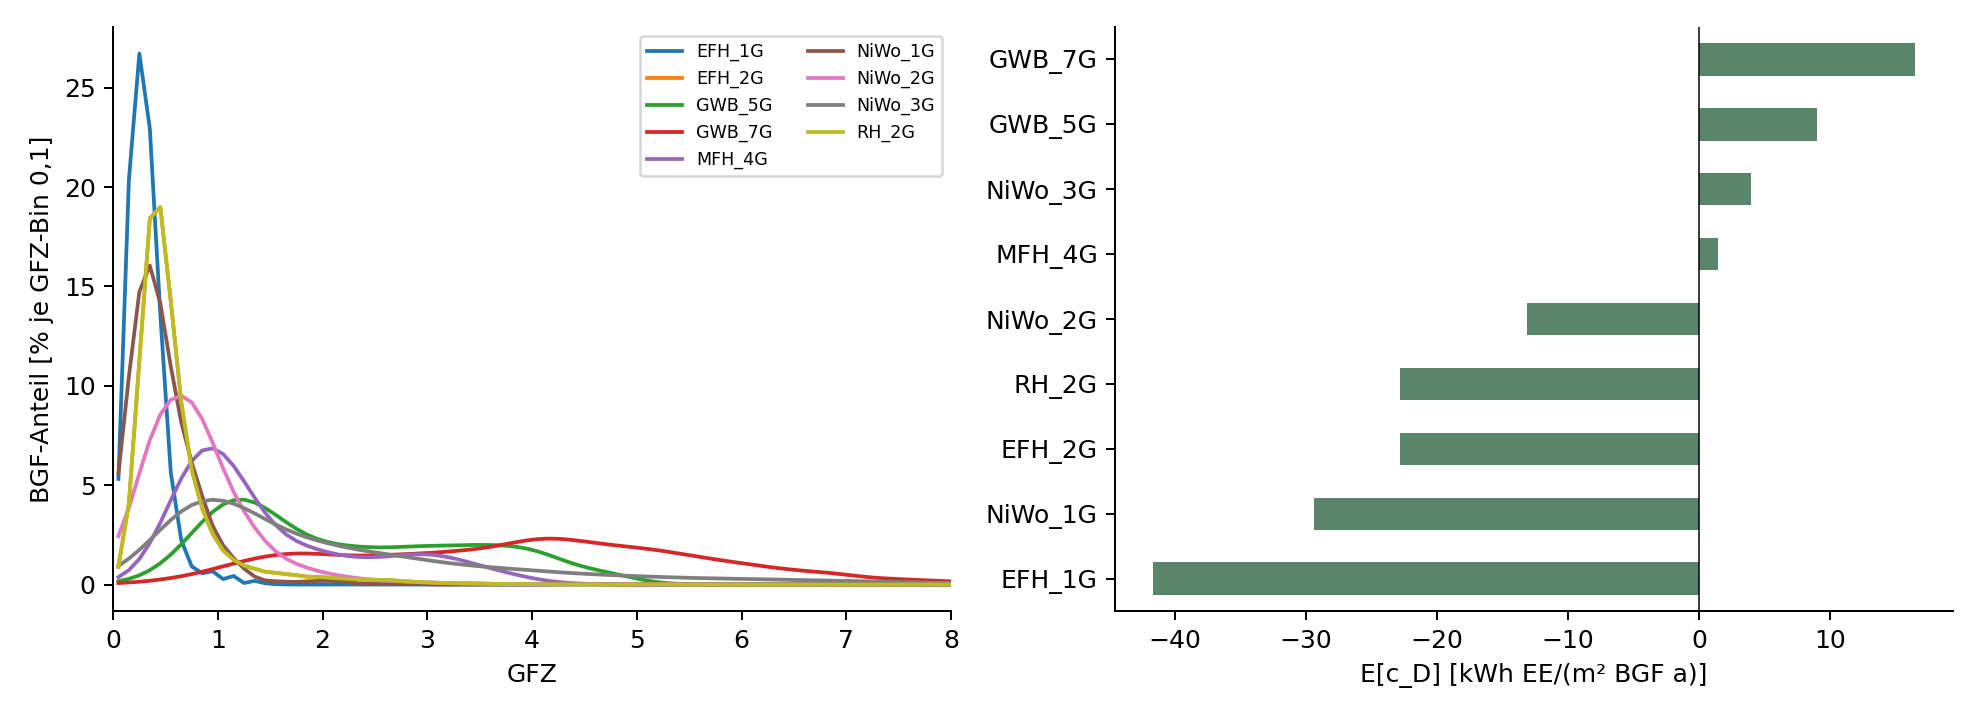
\includegraphics[width=1\linewidth,height=\textheight,keepaspectratio]{Kapitel/../Berechnungen/gebaeudesektormodell/outputs/gfz_dichte.png}

}

\caption{\label{fig-gebaeude-gfz}GFZ-Verteilungen und Erwartungswerte
des historischen Dichte-Referenzansatzes. Die Grafik zeigt GFZ bis 8;
die Aggregation umfasst das vollständige Raster bis 20.}

\end{figure}%

Die Erwartungswerte in Tabelle~\ref{tbl-gebaeude-typologien} werden über
sämtliche GFZ-Bins berechnet. Der Funktionswert am mittleren GFZ wäre
wegen der Nichtlinearität nicht gleichwertig. Als elektrische Referenz
dient die historische Tabellenparametrisierung aus Schneider u.~a.
(2023), Gl. 7 und Tab. 5, mit 30,4, 26,4, Achsenverschiebung 0,15 und
Begrenzung 62. Die gemischte EE-/PE-Beschriftung der Quellentabelle ist
im Notebook dokumentiert; der Referenzansatz ist eine historische
Referenz, keine normative Neufestlegung.

Der Erwartungswert \(\mathbb{E}_k[c_D]\) ist der BGF-gewichtete
Mittelwert des Dichtewerts über die GFZ-Verteilung von Typ \(k\). Der
Index \(j\) bezeichnet einen GFZ-Bin, \(s_{j|k}\) dessen Flächenanteil
und \(d_j\) seine GFZ. Der nationale virtuelle Beitrag lautet
\(C_D=\sum_k A_{BGF,k}\mathbb{E}_k[c_D]\). Positive Werte entlasten die
Bewertungsbilanz, negative erhöhen die Anforderung.

Die virtuellen Erwartungswerte reichen hier von rund \textbf{−41,63 kWh
EE/(m² BGF·a)} für EFH\_1G bis \textbf{+16,44 kWh EE/(m² BGF·a)} für
GWB\_7G. Sie zeigen die Verteilung zusätzlicher Anforderungen und
Gutschriften. Sie werden nicht als reale Stromerzeugung oder als
pauschal zustehende Gutschrift aller Typen bilanziert.

Die Auswahl enthält alle 900 Typen, gegliedert nach Geometrie; der
Achsenregler zeigt einen lesbaren Ausschnitt. Der Tooltip nennt Archetyp
und nationale Fläche. Bedarf wird negativ, PV positiv und die virtuelle
Dichtekorrektur schraffiert gezeigt. MFH\_2G besitzt keine zugeordnete
GFZ-Verteilung und keine nationale Fläche; sein Kontextwert bleibt leer.

\section{Gemeinsame Typologie-Dichte-Matrix und sektoraler
Abgleich}\label{gemeinsame-typologie-dichte-matrix-und-sektoraler-abgleich}

Für Typologie \(k\) und GFZ-Bin \(j\) gilt:

\begin{equation}\protect\phantomsection\label{eq-typologie-gfz-flaeche}{
A_{k,j}^{2040}=A_k^{2040}s_{j|k},\qquad\sum_j s_{j|k}=1.
}\end{equation}

Die erzeugte Typologie-Dichte-Matrix erhält die Fläche jedes positiv
gewichteten Typs. Sie steht im Modellordner unter
\texttt{outputs/typologie\_gfz\_2040.csv.gz} zur Verfügung. Die
Referenzverteilung von 2021 wird dafür als räumliches Verteilungsmuster
verwendet, nicht als zusätzliche Flächensumme.

\begin{longtable}[]{@{}llll@{}}
\caption{Vergleich bei gleichen elektrischen Bilanzgrenzen;
Top-down-Zuordnungen gemäß dokumentiertem
Referenzfall.}\label{tbl-gebaeude-abgleich}\tabularnewline
\toprule\noalign{}
Größe & Bottom-up {[}PJ/a{]} & Top-down {[}PJ/a{]} & Differenz
{[}PJ/a{]} \\
\midrule\noalign{}
\endfirsthead
\toprule\noalign{}
Größe & Bottom-up {[}PJ/a{]} & Top-down {[}PJ/a{]} & Differenz
{[}PJ/a{]} \\
\midrule\noalign{}
\endhead
\bottomrule\noalign{}
\endlastfoot
PV-Erzeugung & 78,245 & 149,000 & -70,755 \\
Gebäudestrombedarf & 137,493 & 108,000 & 29,493 \\
Betrieblicher Stromsaldo & -59,248 & 41,000 & -100,248 \\
Saldo einschließlich MIV & -107,248 & -7,000 & -100,248 \\
\end{longtable}

Die dritte Vergleichsgruppe addiert die historische Dichtefunktion
rechnerisch über \textbf{alle positiv gewichteten Typen}. Das ergibt
einen virtuellen Beitrag von −57,81 PJ-Äquivalent/a: Der betriebliche
Bewertungssaldo beträgt damit −117,06 PJ-Äquivalent/a und einschließlich
derselben MIV-Zuordnung −165,06 PJ-Äquivalent/a. Die physischen
Energieflüsse bleiben unverändert. Diese vollständige Anwendung ist ein
transparenter Vergleichsfall; sie ersetzt keine Festlegung der
PEQ-berechtigten Flächenanteile.

Der Abstand zum Top-down-Saldo beträgt \textbf{−100,25 PJ/a}. Er ergibt
sich aus geringerer PV-Erzeugung und höherem Gebäudestrombedarf des
gelieferten Pools. Werden auf beiden Seiten dieselben 24 PJ/a MIV-Budget
und 72 PJ/a MIV-Bedarf angesetzt, bleibt diese Differenz unverändert.
Sie ist ein Szenariounterschied und wird nicht durch nachträgliche
Flächenskalierung oder eine neue Gutschrift geschlossen.

Für die Kalibrierung in Kapitel~\ref{sec-kalibrierung} fehlen die
definierten PEQ-Flächenanteile, die abgestimmte Versorgung der übrigen
Typen sowie alternative PV-/Flexibilitätsvarianten. Die gelieferte
Typologiematrix und ihre Ergebnisse bilden die Grundlage für diese
Entscheidungen. Die THG-Allokation erhält dadurch nicht automatisch eine
neue Flächenbasis.

\chapter{Kalibrierung der
PEQ-Energieanforderungen}\label{sec-kalibrierung}

Nationale Zielbilanz, neue Gebäudetypologien und dichteabhängige
Anforderungen in Übereinstimmung bringen

Die sektorale Allokation legt den nationalen Referenzsaldo für den
Gebäudesektor fest (Kapitel~\ref{sec-allokation}). Die Gebäude- und
Dichteverteilung definiert, \textbf{welche Flächen} zur Erfüllung dieses
Ziels beitragen (Kapitel~\ref{sec-gebaeudebestand}). Gegenstand dieses
Kapitels ist die Kalibrierung der \textbf{typologie- und
dichteabhängigen PEQ-Anforderungen}. Das Ziel ist keine beliebige
positive Bilanz jedes einzelnen Gebäudes: Die Summe der konsistent
umgerechneten, flächengewichteten Beiträge muss mit dem national
zugewiesenen Ziel vereinbar sein.

Der Dichtefaktor verteilt die Anforderungen zwischen unterschiedlichen
baulichen Dichten. Die Sanierungsanpassung wird \textbf{nach
energetischer Gebäudetypologie} festgelegt und im selben Modell
abgestimmt. Eine allgemeine, von der Typologie unabhängige
Pauschalgutschrift gehört nicht zur neuen Kalibrierung.

\section{Bilanzfunktionen der
Gebäudetypologien}\label{sec-typologiesalden}

Für jede neue energetische Typologie \(k\) werden die relevanten
jährlichen Bedarfe, Erzeugungsannahmen, Bewertungsgrenzen und
Anforderungsparameter aus dem Gebäudeszenario beziehungsweise der
Kalibrierung dokumentiert. Dabei ist zwischen zwei Rollen zu
unterscheiden: \textbf{Nicht-PEQ-Klassen} gehen mit ihrem begründeten,
szenariotypischen Bilanzbeitrag in die nationale Aggregation ein; für
\textbf{PEQ-Klassen} wird die erforderliche Bilanzqualität als
Zielwertfunktion bestimmt. Eine bestimmte PV-Ausstattung oder ein
spezifischer Energiebedarf ist nicht automatisch bereits ein allgemein
geltender PEQ-Grenzwert.

Die Typologieparameter werden in einer versionierten Tabelle
zusammengeführt. Zu klären ist dabei insbesondere, ob ein typologischer
Zielsaldo bereits einen Sanierungsvorteil enthält. In diesem Fall darf
derselbe Vorteil nicht ein zweites Mal als zusätzliche
Sanierungsgutschrift verbucht werden.

\begin{longtable}[]{@{}
  >{\raggedright\arraybackslash}p{(\linewidth - 4\tabcolsep) * \real{0.3333}}
  >{\raggedright\arraybackslash}p{(\linewidth - 4\tabcolsep) * \real{0.3333}}
  >{\raggedright\arraybackslash}p{(\linewidth - 4\tabcolsep) * \real{0.3333}}@{}}
\caption{Parametrisierung der neuen Energieanforderungen.
Typologiespezifische Zielsalden und Kontextgutschriften sind nicht
doppelt zu erfassen.}\label{tbl-kalibrierparameter}\tabularnewline
\toprule\noalign{}
\begin{minipage}[b]{\linewidth}\raggedright
Parameter
\end{minipage} & \begin{minipage}[b]{\linewidth}\raggedright
Bedeutung
\end{minipage} & \begin{minipage}[b]{\linewidth}\raggedright
Status
\end{minipage} \\
\midrule\noalign{}
\endfirsthead
\toprule\noalign{}
\begin{minipage}[b]{\linewidth}\raggedright
Parameter
\end{minipage} & \begin{minipage}[b]{\linewidth}\raggedright
Bedeutung
\end{minipage} & \begin{minipage}[b]{\linewidth}\raggedright
Status
\end{minipage} \\
\midrule\noalign{}
\endhead
\bottomrule\noalign{}
\endlastfoot
\(k\), \(A_{k,j}^{2040}\) & Gebäudetyp und Fläche nach GFZ-Klasse & Aus
Kapitel~\ref{sec-gebaeudebestand} \\
\(e_k\), \(p_k\) & Typologiebezogener Energiebedarf und lokale Erzeugung
& Gelieferte PV30/noFlex-Kennwerte in
Anhang~\ref{sec-gebaeudesektormodell} \\
\(b_{k,j}^{\mathrm{ref}}\) & Modellierter Referenzsaldo für
Nicht-PEQ-Klassen & Aus Szenarioannahmen zu bestimmen \\
\(t_{k,j}^{\mathrm{PEQ}}\) & Zu kalibrierender Mindestbeitrag für
PEQ-Klassen & Neu zu kalibrieren \\
\(c_{\mathrm{S},k}\) & \textbf{Typologiespezifische Sanierungsanpassung}
für die jeweils berechtigte PEQ-Klasse & Neu zu kalibrieren \\
\(c_{\mathrm{D}}(d;\theta)\) & Dichteabhängige Zielwertkorrektur & Neu
zu kalibrieren \\
\(\theta\) & Parameter der Lastenverteilung und gegebenenfalls weitere
Nebenbedingungen & Gemeinsam festzulegen \\
\end{longtable}

\section{Kontextfaktor Dichte: Begründung und physikalisches
Prinzip}\label{sec-kontext-dichte}

Mit zunehmender baulicher Dichte steigt der Energiebedarf näherungsweise
mit der genutzten Geschossfläche, während die für lokale erneuerbare
Erzeugung verfügbaren Dach-, Fassaden- und Grundstücksflächen
vergleichsweise knapp werden. Eine einheitlich geforderte positive
physische Jahresbilanz würde daher niedrig verdichtete Projekte häufig
begünstigen und hohe städtebauliche Dichten benachteiligen. Die
GFZ-basierte Anpassung vermeidet, dass kompakte Siedlungsformen allein
wegen ihrer kleineren lokalen Erzeugungsflächen als weniger ambitioniert
gelten (Fellner u.~a. 2020; Schöfmann u.~a. 2020; Schneider u.~a. 2023).

\begin{figure}

\centering{

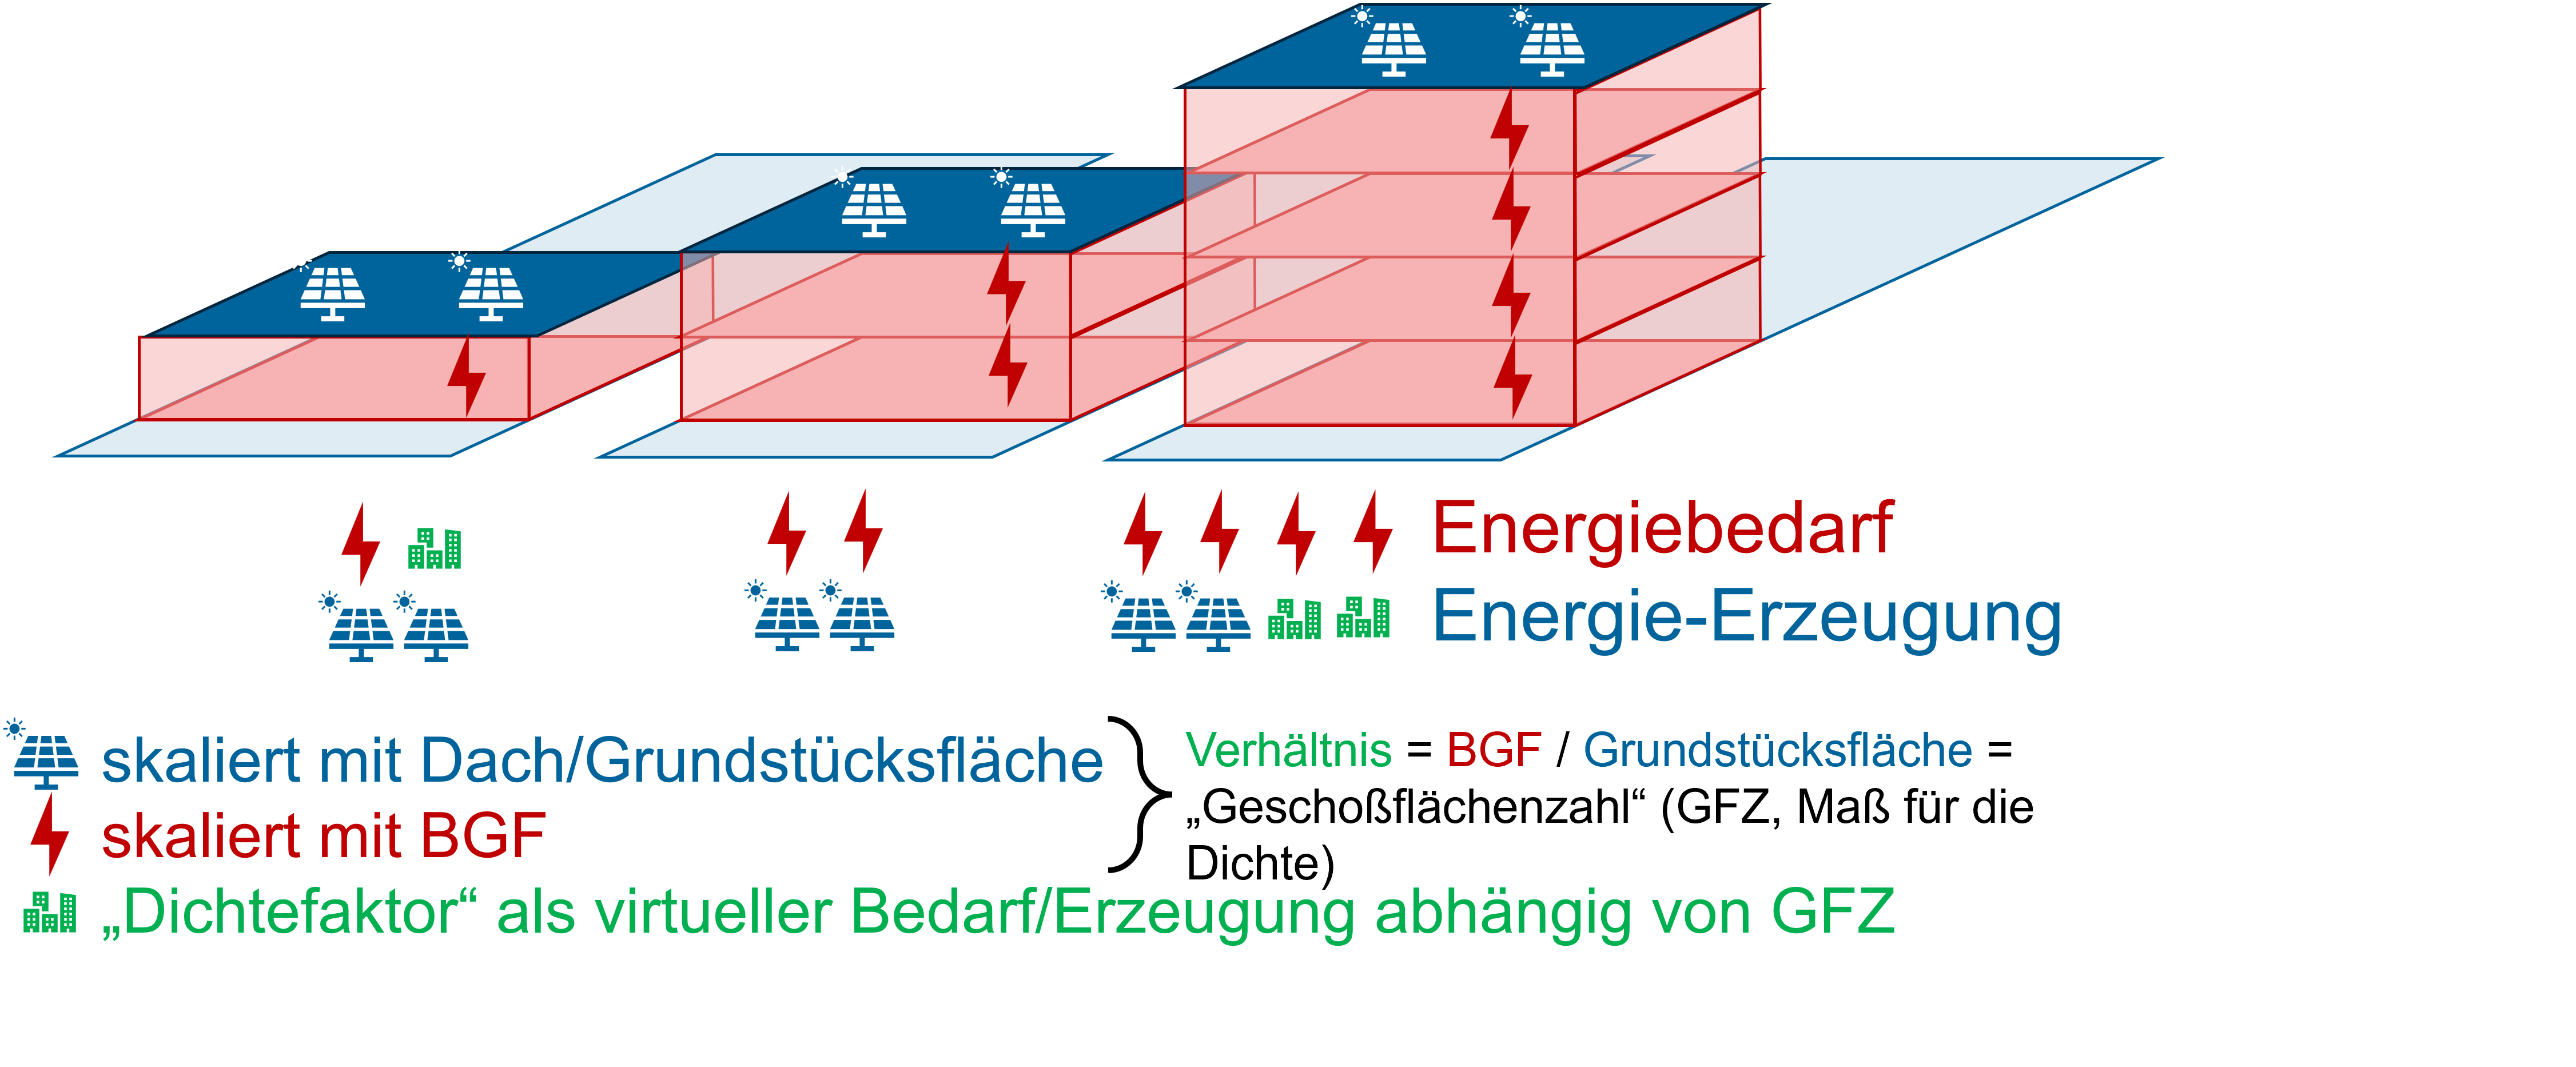
\includegraphics[width=0.95\linewidth,height=\textheight,keepaspectratio]{Kapitel/../Abbildungen/dichte_prinzip2.png}

}

\caption{\label{fig-dichte-prinzip}Zusammenhang zwischen baulicher
Dichte, verfügbarer Erzeugungsfläche und spezifischem Energiepotenzial.}

\end{figure}%

Sei \(A_G\) die Grundstücksfläche, \(A_B\) die Bruttogrundfläche und
\(d=A_B/A_G\) die GFZ. Bei einem Erzeugungspotenzial \(p\) je
Grundstücksfläche und einem Bedarf \(e\) je BGF ergibt sich schematisch:

\begin{equation}\protect\phantomsection\label{eq-dichte-prinzip}{
b(d)=\frac{pA_G-eA_B}{A_B}=\frac{p}{d}-e.
}\end{equation}

Die Gleichung beschreibt den physikalischen Zusammenhang; die
Anforderung folgt aus der nationalen Kalibrierung. Eine Zielwertfunktion
kann durch Parameter, eine Verschiebung der Dichteachse und eine
Begrenzung der Gutschrift den Zusammenhang in eine
Lastenverteilungsregel übersetzen. Die Parameter sind anhand der
nationalen Gebäudeverteilung und Zielbilanz festzulegen (Schneider u.~a.
2023, Gl. 7--8). Gebäudeform, Verschattung, Dach- und Fassadennutzung
bleiben Gegenstand der tatsächlichen Quartiersbilanz.

\begin{figure}

\centering{

\pandocbounded{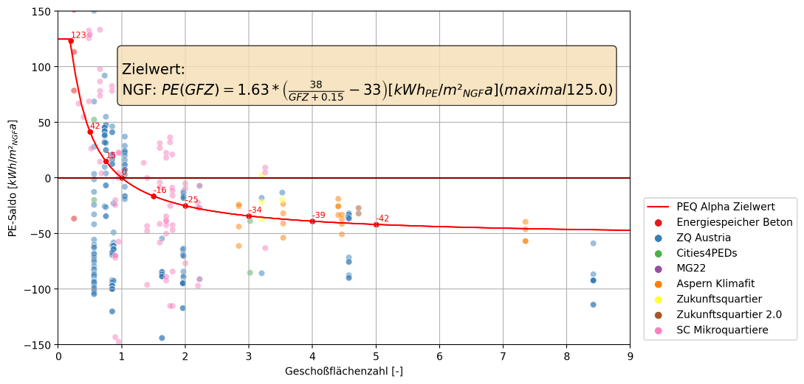
\includegraphics[keepaspectratio]{Kapitel/../Abbildungen/dichte_datenpunkte.png}}

}

\caption{\label{fig-dichte-datenpunkte}Illustration des Zusammenhangs
zwischen technischem Energiepotenzial und baulicher Dichte.}

\end{figure}%

\section{Parametrisierung der Zielwert- und
Gutschriftenfunktion}\label{parametrisierung-der-zielwert--und-gutschriftenfunktion}

Bei der Neubestimmung der Funktion ist zwischen dem unveränderten
\textbf{physikalisch errechneten Quartierssaldo} und den
\textbf{virtuellen Zielwertkorrekturen} zu unterscheiden. Für eine
PEQ-berechtigte Typologie \(k\) lautet die Bewertungsbedingung
schematisch:

\begin{equation}\protect\phantomsection\label{eq-zielwert-typologie}{
b_{\mathrm{PE,phys}}-t_{k,0}^{\mathrm{PE}}
+c_{\mathrm{D}}(d;\theta)+c_{\mathrm{S},k}(\theta)>0.
}\end{equation}

Bei positiv definierter Gutschrift kann man dies äquivalent als
Mindestanforderung an die reale, noch nicht kontextkorrigierte Bilanz
schreiben:

\[
b_{\mathrm{PE,phys}}>
 t_{k,0}^{\mathrm{PE}}-c_{\mathrm{D}}(d;\theta)-c_{\mathrm{S},k}(\theta).
\]

Dabei ist \(t_{k,0}^{\mathrm{PE}}\) das einheitlich definierte
Basiskriterium der betroffenen PEQ-Klasse; bei einem Nullmaßstab ist es
null. Diese Gleichungen definieren die \textbf{Parameterstruktur} des
Entwurfs. Vor einer Festlegung sind Dichteachsenverschiebung,
Begrenzungen, Typologiezuordnung und Nebenbedingungen abzustimmen. Für
Nicht-PEQ-Klassen werden stattdessen die prognostizierten Bilanzbeiträge
dokumentiert. Mobilität wird nicht als frei wählbarer Kalibrierrest in
die Dichtefunktion eingerechnet: Das nationale MIV-Budget entsteht in
Kapitel~\ref{sec-allokation} und wird in
Kapitel~\ref{sec-kontext-mobilitaet} verwendet.

Für die Sanierungsanpassung gilt ausdrücklich: \textbf{kein
einheitlicher Faktor für sämtliche sanierten Flächen}. Der Wert
\(c_{\mathrm{S},k}\) hängt von der zugewiesenen Typologie ab und wird
mit deren energetischen Annahmen und nationalem Flächenanteil gemeinsam
kalibriert. Ob für bestimmte Klassen der Anpassungswert null ist und wie
unterschiedliche Sanierungsintensitäten bewertet werden, ist anhand der
neuen Excel-Klassen fachlich zu begründen.

\section{Nationale Aggregation und
Kalibrierbedingung}\label{nationale-aggregation-und-kalibrierbedingung}

Die Flächenverteilung nach Typologie \(k\) und Dichteklasse \(j\) wird
aus Kapitel~\ref{sec-gebaeudebestand} übernommen. Ein konsistent auf
\textbf{BGF} bezogener jährlicher nationaler Modellbeitrag lässt sich in
den \textbf{fest vorgegebenen Beitrag der Nicht-PEQ-Klassen} und die
\textbf{kalibrierten Beiträge der PEQ-Klassen} zerlegen:

\begin{equation}\protect\phantomsection\label{eq-sektor-aggregation}{
B_{\mathrm{Sektor}}^{\mathrm{Modell}}(\theta)
=\sum_{k\in\mathrm{NichtPEQ}}\sum_j A_{k,j}^{2040}\,b_{k,j}^{\mathrm{ref}}
+\sum_{k\in\mathrm{PEQ}}\sum_j A_{k,j}^{2040}\,t_{k,j}^{\mathrm{PEQ}}(\theta).
}\end{equation}

Die Beiträge werden als jährliche elektrische Energie je BGF aggregiert.
Für NGF-bezogene Kennwerte gilt der dokumentierte Flächenfaktor; die
PE-Bewertung folgt getrennt in der Quartiersbilanz.

Die Parameter \(\theta\) werden so gewählt, dass sich der nationale
aggregierte Zielbeitrag und der aus Kapitel~\ref{sec-allokation}
stammende, in dieselbe Bilanzgröße überführte Referenzsaldo innerhalb
einer ausgewiesenen Toleranz entsprechen:

\begin{equation}\protect\phantomsection\label{eq-kalibrierziel}{
B_{\mathrm{Sektor}}^{\mathrm{Modell}}(\theta)
\stackrel{!}{=}B_{\mathrm{Geb,Ziel}}^{\mathrm{Transition\ 2040}}.
}\end{equation}

Die Bilanzgleichheit allein legt die Parameter nicht notwendigerweise
eindeutig fest. Zusätzliche Bedingungen -- etwa begründete Grenzen der
Dichtefunktion, technologische Potenziale, typologische Zielqualitäten
und vertretbare Sanierungsanforderungen -- müssen ausdrücklich angegeben
werden. Die Verteilung der Gebäudequalitäten und ihre Flächenanteile
sind daher nicht bloß eine Rechenhilfe, sondern zentrale
Szenarioannahmen.

\section{Kalibrierungsstand und
Ergebnisvergleich}\label{kalibrierungsstand-und-ergebnisvergleich}

Unter den Annahmen des Referenzfalls ergeben sich 24 PJ/a elektrisches
MIV-Budget und −7 PJ/a für den Gebäudesektorsaldo einschließlich MIV
(Kapitel~\ref{sec-allokation-ergebnisse}). Die Bottom-up-Rechnung
umfasst 603 positiv gewichtete Typen, ihre GFZ-Verteilungen und die
Erwartungswerte der historischen Dichtefunktion
(Anhang~\ref{sec-gebaeudesektormodell}).

Der physische Pool-Stromsaldo beträgt −59,25 PJ/a. Einschließlich
derselben einmaligen MIV-Zuordnung ergibt sich −107,25 PJ/a, also
−100,25 PJ/a gegenüber dem Top-down-Beispiel. Die virtuellen
Dichte-Erwartungswerte werden dabei nicht als reale Deckung
hinzuaddiert. Der Pool enthält nur PV30/noFlex sowie erhebliche Gas- und
Ölmengen. Eine neue Zielwertfunktion lässt sich deshalb nicht allein
durch Gleichsetzen dieses Pool-Ergebnisses mit dem nationalen Ziel
bestimmen. PEQ-Flächenanteile, energetische Entwicklung der übrigen
Typen und alternative PV-Ausstattungen sind zuerst festzulegen.

\begin{tcolorbox}[enhanced jigsaw, arc=.35mm, bottomrule=.15mm, bottomtitle=1mm, breakable, colback=white, colbacktitle=quarto-callout-note-color!10!white, colframe=quarto-callout-note-color-frame, coltitle=black, left=2mm, leftrule=.75mm, opacityback=0, opacitybacktitle=0.6, rightrule=.15mm, title=\textcolor{quarto-callout-note-color}{\faInfo}\hspace{0.5em}{Geltungsbereich des Entwurfs}, titlerule=0mm, toprule=.15mm, toptitle=1mm]

Die 2040-Flächenmatrix, Energieaggregation und GFZ-Zuordnung sind
berechnet. Die historische Dichtefunktion wird als Referenzansatz
ausgewertet. PEQ-Flächenanteile, Versorgungspfade, PE-Faktorversion und
typologische Sanierungswerte sind nicht normativ festgelegt. Der
Ergebnisvergleich beschreibt diesen Parameterstand.

\end{tcolorbox}

Die Ergebnisdarstellung umfasst Flächen, Typenbeiträge, Dichtekorrektur
und den Abstand zum Referenzsaldo (Kapitel~\ref{sec-gebaeude-abgleich}).
Quelldateien und Parameter sind in den Rechenanhängen versioniert.

\section{Sensitivitäten und normative
Entscheidungen}\label{sensitivituxe4ten-und-normative-entscheidungen}

Neben dem Referenzfall sind insbesondere Änderungen der
Gebäude-PV-Allokation, der Flächenanteile der Gebäudetypen, der
GFZ-Verteilung sowie der typologiebezogenen Sanierungsparameter als
Sensitivitäten sinnvoll. Auch Änderungen des Umfangs der
MIV-/ÖPNV-Zuordnung wirken über Kapitel~\ref{sec-allokation} auf das
nationale Zielbild. Solche Varianten sind vom \textbf{freigegebenen
Referenzszenario} klar zu unterscheiden.

\begin{tcolorbox}[enhanced jigsaw, arc=.35mm, bottomrule=.15mm, bottomtitle=1mm, breakable, colback=white, colbacktitle=quarto-callout-note-color!10!white, colframe=quarto-callout-note-color-frame, coltitle=black, left=2mm, leftrule=.75mm, opacityback=0, opacitybacktitle=0.6, rightrule=.15mm, title=\textcolor{quarto-callout-note-color}{\faInfo}\hspace{0.5em}{Historische Einordnung}, titlerule=0mm, toprule=.15mm, toptitle=1mm]

Die ursprüngliche Kalibrierung verwendete fünf energetische
Gebäudeklassen und eine spezifische Dichtefunktion (Schneider u.~a.
2023). Diese historische Lösung erläutert die Entstehung der Methode,
ersetzt aber weder die neuen Typologien noch die Kalibrierung mit UBA
Transition 2040.

\end{tcolorbox}

\chapter{Kontextfaktor Mobilität}\label{sec-kontext-mobilitaet}

Das in der sektoralen Allokation ermittelte MIV-Budget nutzungsbezogen
verteilen und mit dem örtlichen Mobilitätsbedarf vergleichen

Die nationale \textbf{Höhe} des erneuerbaren MIV-Budgets wird bereits in
Kapitel~\ref{sec-allokation} aus der verfügbaren zentralen,
nicht-PV-basierten erneuerbaren Erzeugung und den vorrangigen Bedarfen
-- insbesondere Industrie und ÖPNV -- hergeleitet. Sie ist keine
eigenständige oder nachträglich festgelegte Mobilitätsgutschrift. Dieses
Kapitel beschreibt nur die \textbf{räumliche und nutzungsbezogene
Anwendung} des daraus hervorgehenden Budgets sowie die standortabhängige
MIV-Bedarfsermittlung.

\begin{tcolorbox}[enhanced jigsaw, arc=.35mm, bottomrule=.15mm, bottomtitle=1mm, breakable, colback=white, colbacktitle=quarto-callout-note-color!10!white, colframe=quarto-callout-note-color-frame, coltitle=black, left=2mm, leftrule=.75mm, opacityback=0, opacitybacktitle=0.6, rightrule=.15mm, title=\textcolor{quarto-callout-note-color}{\faInfo}\hspace{0.5em}{quantitative Allokation}, titlerule=0mm, toprule=.15mm, toptitle=1mm]

Kapitel~\ref{sec-allokation-ergebnisse} zeigt den parametrierten
Transition-Referenzfall: 24 PJ/a beziehungsweise 6,667 TWh/a
elektrisches MIV-Budget bei den dort dokumentierten Annahmen. Die volle
Anrechnung der Wasserstoff-Rückverstromung erhöht es im Vergleichsfall
auf 28 PJ/a. Das sind nationale elektrische Zuteilungen, keine neuen
nutzungsbezogenen PE-Gutschriften. PE-Faktoren, Verteilungsschlüssel und
Ziel-Flächen sind dafür nicht gemeinsam festgelegt. Die vollständige
Rechnung steht in Anhang~\ref{sec-allokation-notebook}.

\end{tcolorbox}

\section{Vom nationalen MIV-Budget zur
Nutzung}\label{vom-nationalen-miv-budget-zur-nutzung}

Nach der sektoralen Elektrizitätsallokation wird das budgetfähige
erneuerbare Mobilitätsvolumen mit einem dokumentierten
Primärenergie-Faktorensatz in das nationale PE-Budget überführt.
Anschließend wird es anhand einer begründeten Verteilung des
individuellen Zielverkehrs den Quartiersnutzungen zugeordnet. Die
nationale Verteilung muss insgesamt genau das freigegebene MIV-Budget
ergeben und darf nicht zusätzlich denselben zentralen Strom anderen
Nutzungen gutschreiben.

Für Nutzung \(u\) gilt:

\begin{equation}\protect\phantomsection\label{eq-mobilitaetsbudget}{
c_{\mathrm{M},u}
=\frac{E_{\mathrm{MIV,Budget}}^{\mathrm{PE}}\,s_u}
{A_{\mathrm{NGF},u}^{2040}},
\qquad \sum_u s_u=1.
}\end{equation}

Dabei ist \(s_u\) der Anteil des nationalen Budgets, der dem von Nutzung
\(u\) verursachten beziehungsweise ihr zugeordneten Zielverkehr
zugerechnet wird. Die verwendeten nationalen NGF müssen dem Flächen- und
Nutzungsstand des Kalibrierungsszenarios entsprechen. Es wird zwischen
\textbf{Budgetverteilung je Nutzung} und \textbf{tatsächlicher
Verkehrsvermeidung am Standort} unterschieden.

\begin{tcolorbox}[enhanced jigsaw, arc=.35mm, bottomrule=.15mm, bottomtitle=1mm, breakable, colback=white, colbacktitle=quarto-callout-note-color!10!white, colframe=quarto-callout-note-color-frame, coltitle=black, left=2mm, leftrule=.75mm, opacityback=0, opacitybacktitle=0.6, rightrule=.15mm, title=\textcolor{quarto-callout-note-color}{\faInfo}\hspace{0.5em}{Parameterstand}, titlerule=0mm, toprule=.15mm, toptitle=1mm]

Das nationale elektrische Budget ist berechnet. Nutzungsbezogene
PE-Gutschriften sind für Transition nicht numerisch festgelegt, da
Faktorensatz, Zielverkehrsanteile und Nutzflächen hierfür nicht
gemeinsam bestimmt sind. Die historischen Werte dokumentieren den
Bewertungsstand 2023.

\end{tcolorbox}

\section{Gemischt genutzte Quartiere}\label{gemischt-genutzte-quartiere}

Für ein Quartier mit verschiedenen Nutzungen ergibt sich die
flächengewichtete spezifische Mobilitätsgutschrift:

\begin{equation}\protect\phantomsection\label{eq-mobilitaet-mischnutzung}{
c_{\mathrm{Mobilität}}
=\frac{\sum_u A_{\mathrm{NGF},u}^{\mathrm{Quartier}}c_{\mathrm{M},u}}
{\sum_u A_{\mathrm{NGF},u}^{\mathrm{Quartier}}}.
}\end{equation}

Die gleiche Nutzungszuordnung ist auch für die Ermittlung des
Verkehrsbedarfs anzuwenden. Zusätzliche Nutzfläche begründet nicht
allein einen Bonus, sondern verändert zugleich den zu bilanzierenden
Zielverkehr. Die Mobilitätsgutschrift darf nur zusammen mit dem
entsprechenden MIV-Bedarf in die erweiterte PEQ-Bilanz eingehen
(Kapitel~\ref{sec-kontext}).

\section{Standortabhängiger MIV-Bedarf: Mobilitätsregionen und
Verkehrsleistung}\label{standortabhuxe4ngiger-miv-bedarf-mobilituxe4tsregionen-und-verkehrsleistung}

Der tatsächlich zu bewertende MIV-Bedarf wird nicht mit dem nationalen
Budget gleichgesetzt. Er hängt von den verursachten Wegen, der Nutzung,
den Standortbedingungen, der Verkehrsmittelwahl und der Fahrzeugflotte
ab. Für die standortabhängige Referenzabschätzung werden
Mobilitätsregionen und Verkehrsdaten aus der österreichischen
Mobilitätserhebung verwendet. Ihre Fortschreibung auf den Zielzustand
und mögliche projektbezogene Abweichungen sind gesondert zu begründen.

\begin{figure}

\centering{

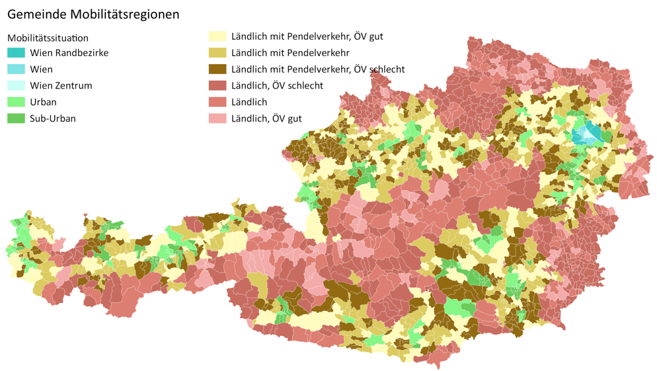
\includegraphics[width=1\linewidth,height=\textheight,keepaspectratio]{Kapitel/../Abbildungen/verkehrsgueteklasse.png}

}

\caption{\label{fig-mobilitaetsregionen}Räumliche Verteilung der
Mobilitätsregionen in Österreich als Grundlage standortabhängiger
Mobilitätsannahmen (Datenquelle: Österreich unterwegs 2013/2014).}

\end{figure}%

\begin{figure}

\centering{

\includegraphics[width=0.9\linewidth,height=\textheight,keepaspectratio]{index_files/mediabag/Kapitel/../Abbildungen/verkehrsleisting.pdf}

}

\caption{\label{fig-miv-verkehrsleistung}Jährliche MIV-Verkehrsleistung
nach Mobilitätsregion (Datenquelle: Österreich unterwegs 2013/2014).}

\end{figure}%

Ein günstiger Standort, kurze Wege, eine hohe ÖV-Güte, gemischte
Nutzungen und ein wirksames Mobilitätskonzept können den MIV-Bedarf
vermindern. Bei gleicher Nutzung und gleichem nationalem Budget erhält
ein Quartier durch solche realen Minderungen einen günstigeren
Bilanzsaldo. Die bloße Bereitstellung einzelner Einrichtungen begründet
noch keine beliebige Verkehrsreduktion.

\section{Abgrenzung von Zielverkehr, Strombedarf und
Ladeprofilen}\label{abgrenzung-von-zielverkehr-strombedarf-und-ladeprofilen}

Für die Quartiersbilanz wird der definierte motorisierte individuelle
\textbf{Zielverkehr} zugeordnet. Für die energetische Simulation von
Lade- und Speicherflüssen sind hingegen reale Anwesenheit und
Ladevorgänge maßgeblich. Ein rechnerisches nationales Mobilitätsbudget
stellt weder eine lokale Stromerzeugungsanlage noch verfügbare
Ladeleistung oder Batteriekapazität dar. Elektromobilität und flexible
Ladevorgänge können die Energiebilanz und Netzbelastung beeinflussen,
sind aber mit der tatsächlichen stündlichen Simulation nachzuweisen
(Schneider 2026, Abschn. 3.3.4).

\section{Dokumentation und
Aktualisierung}\label{dokumentation-und-aktualisierung}

Die Mobilitätsberechnung benötigt zwei unabhängig überprüfbare
Datenteile: (1) den in Kapitel~\ref{sec-allokation} freigegebenen
nationalen MIV-Restbetrag und dessen PE-Umrechnung; (2) Nutzungsflächen,
Wege-, Modal-Split- und Flottenannahmen zur Budgetverteilung und
Standortbewertung. Ein Wechsel der nationalen Szenarioquelle oder der
Verkehrserhebung erfordert eine nachvollziehbare Neukalibrierung und
darf nicht durch pauschales Skalieren der bisherigen Gutschrift ersetzt
werden.

\begin{tcolorbox}[enhanced jigsaw, arc=.35mm, bottomrule=.15mm, bottomtitle=1mm, breakable, colback=white, colbacktitle=quarto-callout-note-color!10!white, colframe=quarto-callout-note-color-frame, coltitle=black, left=2mm, leftrule=.75mm, opacityback=0, opacitybacktitle=0.6, rightrule=.15mm, title=\textcolor{quarto-callout-note-color}{\faInfo}\hspace{0.5em}{Historischer Bewertungsstand}, titlerule=0mm, toprule=.15mm, toptitle=1mm]

Die ursprüngliche, Streicher-basierte Operationalisierung verwendete ein
primärenergetisches MIV-Budget von 10,68 TWh PE/a und daraus abgeleitete
Gutschriften nach Nutzung (Schneider u.~a. 2023, Tab. 8--9). Diese
Zahlen dienen nur zur historischen Einordnung; die neue Gutschrift ist
aus der \textbf{Transition-2040-Sektorallokation} herzuleiten. Wenn eine
bestehende Toolversion noch historische Werte anwendet, ist das als
gesonderter \emph{Implementierungsstand}, nicht als Ergebnis der
Neukalibrierung, zu kennzeichnen.

\end{tcolorbox}

\chapter{Kontextfaktor Sanierung}\label{sec-kontext-sanierung}

Typologieabhängige Sanierungsanpassungen statt einer pauschalen
Flächengutschrift

Die Sanierungsanpassung berücksichtigt spezifische technische und
bauliche Randbedingungen bestehender Gebäude. In der \textbf{neuen
PEQ-Kalibrierung} wird sie \textbf{je energetischer Gebäudetypologie}
definiert und mit deren Flächenanteilen sowie den übrigen
Energieanforderungen abgestimmt (Kapitel~\ref{sec-gebaeudebestand};
Kapitel~\ref{sec-kalibrierung}). Sie ist damit kein von der nationalen
Gebäudesektorbilanz unabhängiger, allgemeiner Pauschalbonus.

\section{Ableitung aus den neuen
Gebäudetypologien}\label{ableitung-aus-den-neuen-gebuxe4udetypologien}

Die zu betrachtenden Typologien, ihre energetischen Zustände und die
zugehörigen nationalen Flächenanteile werden in
Kapitel~\ref{sec-gebaeudebestand} festgelegt. Für jede Typologie \(k\)
ist zu dokumentieren, ob eine Sanierungsanpassung sachlich
gerechtfertigt ist, welchen zulässigen Kontextwert \(c_{\mathrm{S},k}\)
sie erhält und wie dieser Wert mit den modellierten typologischen
Anforderungen zusammenhängt.

Eine typologiespezifische Anpassung kann insbesondere die im Bestand
eingeschränkten Maßnahmenmöglichkeiten berücksichtigen. Die konkreten
Kriterien -- zum Beispiel Sanierungstiefe, vorhandene Konstruktion und
verbleibender energetischer Bedarf -- sind anhand der neuen Klassen zu
definieren. Die Höhe ist \textbf{Ergebnis der gemeinsamen Kalibrierung},
nicht automatisch der Abstand zu einem Neubau-Bedarfswert und nicht eine
pauschal behauptete CO₂-Einsparung.

\section{Anwendung auf gemischte
Quartiere}\label{anwendung-auf-gemischte-quartiere}

Enthält ein Quartier mehrere nachweisrelevante Gebäudetypologien, kann
der spezifische Kontextwert als nutzflächengewichteter Mittelwert
gebildet werden:

\begin{equation}\protect\phantomsection\label{eq-sanierungskontext}{
c_{\mathrm{Sanierung,typ}}=
\frac{\sum_k A_{\mathrm{NGF},k}^{\mathrm{Quartier}}\,c_{\mathrm{S},k}}
{\sum_k A_{\mathrm{NGF},k}^{\mathrm{Quartier}}}.
}\end{equation}

Voraussetzung ist, dass jede Teilfläche eindeutig einer freigegebenen
Typologie zugeordnet ist. Die Werte sind in kWh PE/(m² NGF·a)
auszudrücken. Die nationalen Eingabeflächen der Kalibrierung können
dagegen BGF sein; die Umrechnung wird in Kapitel~\ref{sec-kalibrierung}
nachvollziehbar dokumentiert. Neubau- und Bestandsflächen werden nicht
allein wegen der Zugehörigkeit zu demselben Quartier gleichbehandelt.

Die Sanierungsanpassung ändert die \textbf{Bewertungsanforderung}, nicht
die tatsächlich simulierten Energieflüsse. Bereits in einem
typologiebezogenen Ausgangsziel berücksichtigte Vorteile dürfen nicht
zusätzlich als Gutschrift angesetzt werden. Erhaltene Bausubstanz und
eingesparte graue Emissionen wirken, soweit methodisch vorgesehen, in
der eigenständigen Lebenszyklus-THG-Bilanz; die Primärenergieanpassung
ist nicht noch einmal eine vermiedene CO₂-Menge.

\begin{tcolorbox}[enhanced jigsaw, arc=.35mm, bottomrule=.15mm, bottomtitle=1mm, breakable, colback=white, colbacktitle=quarto-callout-note-color!10!white, colframe=quarto-callout-note-color-frame, coltitle=black, left=2mm, leftrule=.75mm, opacityback=0, opacitybacktitle=0.6, rightrule=.15mm, title=\textcolor{quarto-callout-note-color}{\faInfo}\hspace{0.5em}{Parameterstand}, titlerule=0mm, toprule=.15mm, toptitle=1mm]

Der Entwurf definiert die typologische Zuordnung und Aggregationsregel.
Numerische Sanierungswerte je Typ sind nicht festgelegt. Die historische
Pauschale ist ausschließlich als Vergleichsstand dokumentiert.

\end{tcolorbox}

\begin{tcolorbox}[enhanced jigsaw, arc=.35mm, bottomrule=.15mm, bottomtitle=1mm, breakable, colback=white, colbacktitle=quarto-callout-note-color!10!white, colframe=quarto-callout-note-color-frame, coltitle=black, left=2mm, leftrule=.75mm, opacityback=0, opacitybacktitle=0.6, rightrule=.15mm, title=\textcolor{quarto-callout-note-color}{\faInfo}\hspace{0.5em}{Historische Einordnung}, titlerule=0mm, toprule=.15mm, toptitle=1mm]

Die bisherige Operationalisierung nutzte eine pauschale
Sanierungsgutschrift von \textbf{15 kWh PE/(m² NGF·a)}, flächenanteilig
angewendet (Schneider u.~a. 2026, 14). Sie wird hier ausschließlich als
früherer Stand genannt und \textbf{nicht} als Regel der neuen
typologischen Kalibrierung fortgeschrieben.

\end{tcolorbox}

\chapter{Zielwert THG}\label{sec-zielwert-thg}

Vom nationalen Klimabudget zum kumulierten Emissionsbudget eines
Quartiers

Der Energiezielwert beschreibt die jährliche Leistung im Zielsystem. Der
THG-Zielwert begrenzt dagegen die kumulierten Emissionen aus Errichtung,
Betrieb, Instandhaltung und MIV über 50 Jahre.

\section{Wie entstehen 320 kg CO₂e je
Quadratmeter?}\label{wie-entstehen-320-kg-coux2082e-je-quadratmeter}

\subsection{Nationale Grundlage und sektorale
Verteilung}\label{nationale-grundlage-und-sektorale-verteilung}

Das Verfahren unterscheidet drei Budgetvarianten. Ausgangspunkte sind
das verbleibende nationale CO₂-Budget, Annahmen über natürliche Senken,
ein Anteil von 50 \% für Gebäude und MIV sowie eine nationale
Bezugsfläche von 906,7 Mio. m² BGF. Der Klimabudgetansatz bezieht sich
auf 1,5 °C mit 66 \% Wahrscheinlichkeit; dokumentiert werden Varianten
mit und ohne temporäre Überschreitung des Temperaturziels (Schneider
u.~a. 2025, Abschn. 2.3, Tab. 2 und A1, S. 6--7, 30).

Die Budgetvarianten L1, L2 und L3 beruhen auf einem Klimabudget
\textbf{ohne temporäre Überschreitung} des Temperaturziels: Von 280 Mt
CO₂ ab 2022 verbleiben nach Abzug der bis Ende 2024 angesetzten
Emissionen 130 Mt ab 2025. Dieses Ausgangsbudget bildet die Referenz der
Bewertung (Schneider u.~a. 2025, Tab. A1).

Mit nationalem Restbudget \(B_{\mathrm{AT}}\), Bevölkerung \(P\),
jährlicher Senkenleistung je Person \(s\), Zeitraum \(T\), Sektoranteil
\(\alpha\) und Bezugsfläche \(A_B\) gilt:

\begin{equation}\protect\phantomsection\label{eq-thg-allokation}{
b_{\mathrm{THG}}
=\frac{\alpha\left(B_{\mathrm{AT}}+P\,s\,T\right)}{A_B}.
}\end{equation}

Budget und Senkenleistung werden in einer gemeinsamen Masseneinheit
angesetzt. Das nationale CO₂-Budget dient als Grundlage für die
Zuteilung; auf Quartiersebene werden die Treibhausgase mit GWP100 in
CO₂-Äquivalenten bewertet.

\begin{longtable}[]{@{}
  >{\raggedright\arraybackslash}p{(\linewidth - 4\tabcolsep) * \real{0.3000}}
  >{\raggedleft\arraybackslash}p{(\linewidth - 4\tabcolsep) * \real{0.4000}}
  >{\raggedright\arraybackslash}p{(\linewidth - 4\tabcolsep) * \real{0.3000}}@{}}
\caption{Eingangsgrößen der THG-Allokation (Schneider u.~a. 2025, Tab.
A1, S. 30).}\label{tbl-thg-eingaben}\tabularnewline
\toprule\noalign{}
\begin{minipage}[b]{\linewidth}\raggedright
Größe
\end{minipage} & \begin{minipage}[b]{\linewidth}\raggedleft
Referenzwert
\end{minipage} & \begin{minipage}[b]{\linewidth}\raggedright
Funktion
\end{minipage} \\
\midrule\noalign{}
\endfirsthead
\toprule\noalign{}
\begin{minipage}[b]{\linewidth}\raggedright
Größe
\end{minipage} & \begin{minipage}[b]{\linewidth}\raggedleft
Referenzwert
\end{minipage} & \begin{minipage}[b]{\linewidth}\raggedright
Funktion
\end{minipage} \\
\midrule\noalign{}
\endhead
\bottomrule\noalign{}
\endlastfoot
Verbleibendes Budget ab 2025 & 130 Mt CO₂ & Ausgangsbudget ohne
zusätzliche Senken \\
Bevölkerung & 9,0 Mio. Personen & Bezug für die Senkenannahme \\
Betrachtungsdauer & 50 Jahre & Kumulation der Senkenannahme \\
Anteil Gebäude und MIV & 50 \% & Sektorale Zuteilung \\
Nationale Bruttogrundfläche im Zieljahr 2040 & 906,7 Mio. m² &
Flächenbezogene Verteilung \\
\end{longtable}

Für L3 werden 1 t CO₂e pro Person und Jahr an natürlichen Senken
angesetzt. Über 50 Jahre und 9 Mio. Personen entsprechen sie 450 Mt.
Zusammen mit dem Ausgangsbudget ergeben sich 580 Mt, davon 290 Mt für
Gebäude und MIV. Geteilt durch 906,7 Mio. m² ergibt dies gerundet
\textbf{320 kg CO₂e/m² BGF}.

\begin{longtable}[]{@{}
  >{\raggedright\arraybackslash}p{(\linewidth - 4\tabcolsep) * \real{0.2727}}
  >{\raggedleft\arraybackslash}p{(\linewidth - 4\tabcolsep) * \real{0.3636}}
  >{\raggedleft\arraybackslash}p{(\linewidth - 4\tabcolsep) * \real{0.3636}}@{}}
\caption{Budgetvarianten nach Schneider et al. (Schneider u.~a. 2025,
Tab. 2, S. 7).}\label{tbl-thg-budgetvarianten}\tabularnewline
\toprule\noalign{}
\begin{minipage}[b]{\linewidth}\raggedright
Variante
\end{minipage} & \begin{minipage}[b]{\linewidth}\raggedleft
Senkenannahme {[}t CO₂e/(Person a){]}
\end{minipage} & \begin{minipage}[b]{\linewidth}\raggedleft
THG-Budget {[}kg CO₂e/m² BGF{]}
\end{minipage} \\
\midrule\noalign{}
\endfirsthead
\toprule\noalign{}
\begin{minipage}[b]{\linewidth}\raggedright
Variante
\end{minipage} & \begin{minipage}[b]{\linewidth}\raggedleft
Senkenannahme {[}t CO₂e/(Person a){]}
\end{minipage} & \begin{minipage}[b]{\linewidth}\raggedleft
THG-Budget {[}kg CO₂e/m² BGF{]}
\end{minipage} \\
\midrule\noalign{}
\endhead
\bottomrule\noalign{}
\endlastfoot
L1 & 0 & 72 \\
L2 & 0,5 & 196 \\
L3 & 1,0 & 320 \\
\end{longtable}

Die L-Werte sind \textbf{Budgetvarianten innerhalb der THG-Bewertung},
nicht die drei PEQ-Qualitätsstufen. Der für diesen Bericht zugrunde
gelegte Zertifizierungswert beträgt 320 kg CO₂e/m² BGF. Seine Einhaltung
ist zusammen mit der L3-Senkenannahme und den Bilanzregeln zu lesen. Die
unterstellte nationale Senkenleistung ist kein vom einzelnen Quartier
nachgewiesener Emissionsausgleich.

\section{Gebäudesektor: Bezugsflächen und
Entwicklung}\label{sec-thg-flaechen}

Die Fläche bestimmt, wie ein nationales Budget auf Quadratmeter verteilt
wird. Die folgenden Datenstände haben unterschiedliche Abgrenzungen; sie
bilden \textbf{keine durchgängige Zeitreihe}. Insbesondere darf aus
ihrer Differenz kein Rückgang des Gebäudebestands abgeleitet werden.

\begin{longtable}[]{@{}
  >{\raggedright\arraybackslash}p{(\linewidth - 6\tabcolsep) * \real{0.2143}}
  >{\raggedleft\arraybackslash}p{(\linewidth - 6\tabcolsep) * \real{0.2857}}
  >{\raggedleft\arraybackslash}p{(\linewidth - 6\tabcolsep) * \real{0.2857}}
  >{\raggedright\arraybackslash}p{(\linewidth - 6\tabcolsep) * \real{0.2143}}@{}}
\caption{Flächenbezüge des Energie- und
THG-Modells.}\label{tbl-thg-flaechenentwicklung}\tabularnewline
\toprule\noalign{}
\begin{minipage}[b]{\linewidth}\raggedright
Datenstand / Horizont
\end{minipage} & \begin{minipage}[b]{\linewidth}\raggedleft
BGF {[}Mio. m²{]}
\end{minipage} & \begin{minipage}[b]{\linewidth}\raggedleft
NGF {[}Mio. m²{]}
\end{minipage} & \begin{minipage}[b]{\linewidth}\raggedright
Rolle und Quelle
\end{minipage} \\
\midrule\noalign{}
\endfirsthead
\toprule\noalign{}
\begin{minipage}[b]{\linewidth}\raggedright
Datenstand / Horizont
\end{minipage} & \begin{minipage}[b]{\linewidth}\raggedleft
BGF {[}Mio. m²{]}
\end{minipage} & \begin{minipage}[b]{\linewidth}\raggedleft
NGF {[}Mio. m²{]}
\end{minipage} & \begin{minipage}[b]{\linewidth}\raggedright
Rolle und Quelle
\end{minipage} \\
\midrule\noalign{}
\endhead
\bottomrule\noalign{}
\endlastfoot
Statistikbezug 2021, GFZ-Hochrechnung & 1.058,935 & 847,1 &
Bestandsverteilung nach Nutzung, Bundesland und Geschossklasse;
Kapitel~\ref{sec-gfz-verteilung}; BGF = NGF / 0,8 \\
Building-Sector Pool, „heute`` (Jahr offen) & 1.112,341 & 889,873 &
Gelieferte Typenflächen; NGF/BGF = 0,8 als Modellannahme;
Kapitel~\ref{sec-gebaeudebestand} \\
Building-Sector Pool, Entwicklung 2040 & 1.126,579 & 901,263 & Neue
Bottom-up-Energieauswertung; keine automatische Änderung der
THG-Budgetfläche \\
Zielbestand 2040 der THG-Kalibrierung & 906,7 & nicht separat angesetzt
& Bezugsfläche der Budgetzuteilung; Schneider u.~a. (2025), Tab. A1 \\
Bestand 2025 und Zwischenjahre bis 2040 & nicht im Datensatz enthalten &
nicht im Datensatz enthalten & Keine interpolierten Werte ohne
harmonisierte Abgrenzung \\
\end{longtable}

\begin{longtable}[]{@{}
  >{\raggedright\arraybackslash}p{(\linewidth - 4\tabcolsep) * \real{0.3333}}
  >{\raggedright\arraybackslash}p{(\linewidth - 4\tabcolsep) * \real{0.3333}}
  >{\raggedright\arraybackslash}p{(\linewidth - 4\tabcolsep) * \real{0.3333}}@{}}
\caption{Datenumfang der
Gebäudeflächenentwicklung.}\label{tbl-thg-fortschreibung}\tabularnewline
\toprule\noalign{}
\begin{minipage}[b]{\linewidth}\raggedright
Baustein der Fortschreibung
\end{minipage} & \begin{minipage}[b]{\linewidth}\raggedright
Benötigte Angaben
\end{minipage} & \begin{minipage}[b]{\linewidth}\raggedright
Aktueller Status
\end{minipage} \\
\midrule\noalign{}
\endfirsthead
\toprule\noalign{}
\begin{minipage}[b]{\linewidth}\raggedright
Baustein der Fortschreibung
\end{minipage} & \begin{minipage}[b]{\linewidth}\raggedright
Benötigte Angaben
\end{minipage} & \begin{minipage}[b]{\linewidth}\raggedright
Aktueller Status
\end{minipage} \\
\midrule\noalign{}
\endhead
\bottomrule\noalign{}
\endlastfoot
Ausgangsbestand & Stützjahr, Nutzung, konditionierte Fläche,
NGF/BGF-Abgrenzung & Statistikmodell 2021 vorhanden; Abgleich mit
THG-Systemgrenze offen \\
Neubau und Erweiterung & Zusätzliche m² je Nutzung und Jahr &
Typengewichteter Neubauanteil 2040 vorhanden; zeitliche Übergangsbilanz
nicht festgelegt (Kapitel~\ref{sec-gebaeude-flaechen}) \\
Abbruch und Umnutzung & Abgänge und Nutzungsverschiebungen je Jahr &
Nicht im Datensatz enthalten \\
Sanierung & Sanierte m² und energetischer Zustand je Jahr & Keine
zusätzliche Geschossfläche allein durch Sanierung unterstellen \\
Zielbestand & Konsistente Summe aus Bestand, Zu- und Abgängen & 906,7
Mio. m² als bestehende Kalibrierungsannahme erhalten \\
\end{longtable}

\section{Drei Zeitbegriffe}\label{drei-zeitbegriffe}

Der Bewertungszeitraum beträgt \textbf{50 Jahre, von 2025 bis 2075}.
Innerhalb dieses Horizonts werden die treibhauswirksamen Effekte
bilanziert.

Die Ableitung orientiert sich am österreichischen Klimaneutralitätsziel
\textbf{2040}; auf dieses Jahr beziehen sich auch die zugrunde gelegten
Flächenprognosen. \textbf{2050} wird als vorsorglich späterer
Dekarbonisierungszeitpunkt angesetzt, um eine mögliche Verzögerung
gegenüber dem ursprünglichen Ziel abzubilden. Damit wird das
Prognosejahr der Bezugsfläche nicht automatisch auf 2050 verschoben.
Eine spätere Umstellung erfordert eine dokumentierte Fortschreibung.

Die vereinfachende Annahme einer vollständigen Dekarbonisierung der
betrachteten Prozesse \textbf{ab 2050} führt dazu, dass danach im Modell
keine zusätzlichen Emissionen mehr entstehen. Das emissionswirksame
Zeitfenster liegt damit faktisch vor 2050, obwohl die Betrachtung bis
2075 reicht. Dies ist eine Szenarioannahme, keine Verkürzung des
Bewertungszeitraums und keine Garantie der tatsächlichen Entwicklung
(Schneider u.~a. 2025, Abschn. 2.4, S. 7--8; Schneider 2026, Abschn.
3.2.8, S. 58--60).

\textbf{GWP100} bezeichnet den 100-jährigen Charakterisierungshorizont
des Treibhauspotenzials für die Bewertung unterschiedlicher
Treibhausgase in CO₂-Äquivalenten. Diese 100 Jahre bestimmen nicht die
Projektlaufzeit.

Errichtungsemissionen beanspruchen das Budget unmittelbar. Eine
rechnerische Verteilung auf 50 Jahresraten würde ihren
Emissionszeitpunkt nicht ändern. Für Etappen eines Renovierungsfahrplans
muss deshalb betrachtet werden, wann bauliche Emissionen entstehen und
welche Betriebsemissionen bis zur jeweiligen Maßnahme anfallen.

\section{Absenkpfade und kumuliertes THG-Budget}\label{sec-thg-pfade}

Für die Lebenszyklusbewertung werden zeitabhängige Emissionsfaktoren
verwendet. Ihre Entwicklung bildet einen angenommenen
Dekarbonisierungspfad ab und beeinflusst insbesondere die Bewertung der
Betriebsemissionen im Szenariozeitraum.

\begin{figure}

\centering{

\includegraphics[width=1\linewidth,height=\textheight,keepaspectratio]{index_files/mediabag/Kapitel/../Abbildungen/absenkpfade.pdf}

}

\caption{\label{fig-absenkpfade}Angenommene Entwicklung der spezifischen
Treibhausgasemissionen verschiedener Energieträger und
Versorgungssysteme bis 2050.}

\end{figure}%

Die bestehende Abbildung unterscheidet Netzstromvarianten,
Fernwärmesysteme, Abwärme sowie fossile und biogene Brennstoffe. Die
numerischen Zeitreihen sind im Datensatz nicht enthalten; die Abbildung
dokumentiert die Szenariopfade qualitativ. Die methodische Grundlage
bilden Schneider u.~a. (2025), Abschn. 2.4 und 2.6, sowie Schneider
(2026), Abschn. 3.2.8.

{\def\LTcaptype{none} % do not increment counter
\begin{longtable}[]{@{}
  >{\raggedright\arraybackslash}p{(\linewidth - 4\tabcolsep) * \real{0.3333}}
  >{\raggedright\arraybackslash}p{(\linewidth - 4\tabcolsep) * \real{0.3333}}
  >{\raggedright\arraybackslash}p{(\linewidth - 4\tabcolsep) * \real{0.3333}}@{}}
\toprule\noalign{}
\begin{minipage}[b]{\linewidth}\raggedright
Größe
\end{minipage} & \begin{minipage}[b]{\linewidth}\raggedright
Anwendung im kumulierten Budget
\end{minipage} & \begin{minipage}[b]{\linewidth}\raggedright
Dokumentierter Stand
\end{minipage} \\
\midrule\noalign{}
\endhead
\bottomrule\noalign{}
\endlastfoot
Netzstrom und weitere Energieträger & Jahresverbrauch × zeitabhängiger
THG-Faktor, über die Jahre summiert & Trägerspezifische Pfade in
Abbildung~\ref{fig-absenkpfade}; numerische Stützwerte und Interpolation
nicht im Datensatz enthalten \\
Herstellung, Ersatz und Lebensende & Emissionen zum jeweiligen
Ereigniszeitpunkt & Prozessbezogene Dekarbonisierungsannahmen des
Referenzverfahrens \\
Vollständige Dekarbonisierung ab 2050 & Im Modell keine zusätzlichen
Emissionen der so erfassten Versorgung und Prozesse & Szenarioannahme,
keine physische Zusicherung; Betrachtung läuft bis 2075 weiter \\
Natürliche Senken & Bestandteil der nationalen Budgetzuteilung & Eigene
Annahme; kein Abzug durch einen fallenden Stromfaktor \\
\end{longtable}
}

\section{Rekalibrierung: Welche Stellgrößen ändern
sich?}\label{rekalibrierung-welche-stellgruxf6uxdfen-uxe4ndern-sich}

Eine Fortschreibung muss klären, ob Datenbasis, Szenario oder
Verteilungsentscheidung verändert werden. Beim THG-Budget sind
Restbudget, Senkenannahme, Sektoranteil und Bezugsfläche maßgeblich.
Diese Größen sind bei einer Rekalibrierung gemeinsam zu überprüfen
(Schneider u.~a. 2025, Abschn. 4.2--4.3, S. 27--28).

Zusätzlicher Baubedarf kann eine Entscheidung über die sektorale
Verteilung auslösen. Ein höheres Budget je Quadratmeter entsteht daraus
nicht von selbst: Bei unverändertem Sektorbudget verteilt sich dieselbe
Menge auf mehr Fläche. Soll der Gebäudesektor mehr Budget erhalten, muss
die entsprechende Entlastung anderer Sektoren oder eine begründete
Änderung der Budgetgrundlage ausgewiesen werden. Eine Erhöhung ohne
solche Deckung verändert den Gesamtanspruch.

\subsection{PV-Errichtung und sektorale
Konsistenz}\label{pv-errichtung-und-sektorale-konsistenz}

Die grauen Emissionen der PV-Anlagen bleiben außerhalb der
Quartiersbilanz, weil die Erzeugungsanlagen im nationalen Sektormodell
der Energieversorgung zugeordnet sind. Diese Abgrenzung setzt voraus,
dass ihre Emissionen dort konsistent erfasst werden (Schneider u.~a.
2025, Abschn. 2.4.1 und 4.2, S. 8--9, 27--28).

Eine Alternative nimmt die PV-Errichtung in die Quartiersbilanz auf.
Dann müssen Emissionen und Budgetzuordnung gemeinsam neu abgegrenzt
werden. Eine zusätzliche Belastung bei unverändertem, anders
abgegrenztem Budget würde zwei Bilanzmodelle vermischen. Wie sich die
konsistente Alternative auf Grenzwert und Vorteil zusätzlicher PV
auswirkt, ist zu berechnen. Kapitel~\ref{sec-bilanzregeln} erläutert die
Abgrenzung der PV-Errichtung und die Voraussetzungen eines Vergleichs
mit einer gebäudebezogenen Normbilanz.

\section{Folgerungen für Planung und
Verwaltung}\label{folgerungen-fuxfcr-planung-und-verwaltung}

Die Allokation zeigt, welche Beiträge ein Quartier selbst erbringen soll
und welche Voraussetzungen es aus dem übergeordneten System übernimmt.
Ein Nachweis sollte deshalb neben dem Ergebnis den Methodenstand, die
Systemgrenzen, Flächenbezüge und Kontextgutschriften ausweisen. Erst
damit lässt sich unterscheiden, ob eine Verbesserung aus einer
Planungsmaßnahme, einer geänderten Annahme oder einem anderen
Bewertungsmaßstab stammt.

\chapter{Systemgrenze des Quartiers}\label{sec-bilanzregeln}

Was gehört zur Quartiersbilanz -- und wie werden Energieflüsse und
Emissionen bewertet?

Die Aussage einer Energie- oder Treibhausgasbilanz hängt wesentlich
davon ab, \textbf{was einbezogen, wie zugeordnet und über welchen
Zeitraum bewertet wird}. Der klimaaktiv Standard legt deshalb räumliche,
funktionale und zeitliche Systemgrenzen fest. Diese gelten für
Energiebedarf, erneuerbare Erzeugung, Mobilität und
Lebenszyklusemissionen ebenso wie für die zugehörigen Zielwerte und
Kontextfaktoren.

Die drei Qualitätsstufen und ihre Erfüllungskriterien werden im Kapitel
Kapitel~\ref{sec-standard} eingeführt. Dieses Kapitel erläutert die
\textbf{konkreten Bilanzierungsregeln}. Die nationale Herleitung der
Anforderungen steht in Kapitel~\ref{sec-allokation} und
Kapitel~\ref{sec-zielwert-thg}; ihre kontextabhängige Anwendung in
Kapitel~\ref{sec-kontext}.

\section{Räumliche Systemgrenze: Was gehört zum
Quartier?}\label{ruxe4umliche-systemgrenze-was-gehuxf6rt-zum-quartier}

Das bewertete Quartier wird als räumlich und funktional zusammenhängende
Einheit abgegrenzt. Zum Projektumfang gehören die einbezogenen Gebäude,
ihre zugehörigen Flächen sowie gemeinschaftliche Versorgungs- und
Erzeugungsanlagen. Auch unbeheizte Gebäudeteile, Keller und zugehörige
Außenanlagen können für die bauliche Treibhausgasbilanz relevant sein,
selbst wenn sie nicht zur konditionierten Nutzfläche zählen (Schneider
2026, Abschn. 3.2.2, S. 51--53).

\begin{tcolorbox}[enhanced jigsaw, arc=.35mm, bottomrule=.15mm, bottomtitle=1mm, breakable, colback=white, colbacktitle=quarto-callout-important-color!10!white, colframe=quarto-callout-important-color-frame, coltitle=black, left=2mm, leftrule=.75mm, opacityback=0, opacitybacktitle=0.6, rightrule=.15mm, title=\textcolor{quarto-callout-important-color}{\faExclamation}\hspace{0.5em}{Wichtig}, titlerule=0mm, toprule=.15mm, toptitle=1mm]

Die Grenze darf nicht allein mit dem Ziel gewählt werden, günstige
Erzeugungsflächen einzuschließen oder besonders energieintensive
Nutzungen auszuklammern. Bei Anlagen, die mehrere Gebäude oder auch
Bereiche außerhalb des Quartiers versorgen, muss die \textbf{Zuordnung
der Energieflüsse und baulichen Aufwendungen} nachvollziehbar sein.

\end{tcolorbox}

Für die Bewertung sind insbesondere folgende Bezugsgrößen zu
dokumentieren:

\begin{itemize}
\tightlist
\item
  \textbf{Grundstücks- beziehungsweise Quartiersfläche:} maßgeblich für
  die räumliche Abgrenzung und die Geschoßflächenzahl (GFZ).
\item
  \textbf{Bruttogrundfläche (BGF):} Bezugsgröße des kumulierten
  THG-Budgets und Bestandteil der GFZ.
\item
  \textbf{Konditionierte Nettogrundfläche (NGF):} Bezugsgröße der
  spezifischen betrieblichen Primärenergiebilanz.
\item
  \textbf{Nutzungsanteile:} Grundlage für Bedarfsprofile und die
  flächengewichtete Zuordnung von Mobilitätsbudgets.
\end{itemize}

\section{Funktionale Bilanzgrenze: Welche Nutzungen und Prozesse
zählen?}\label{funktionale-bilanzgrenze-welche-nutzungen-und-prozesse-zuxe4hlen}

Der Umfang der Bewertung steigt mit der angestrebten Qualitätsstufe. Der
Gebäudebetrieb ist Bestandteil aller Stufen; bei den beiden erweiterten
Stufen kommt der zugeordnete motorisierte Individualverkehr (MIV) hinzu.
Erst die Klimaneutralitätsstufe verlangt darüber hinaus die Einhaltung
eines kumulierten THG-Budgets einschließlich der definierten baulichen
Lebenszyklusprozesse (Schneider u.~a. 2025, Tab. 1; Schneider u.~a.
2026, 8--11).

Für die Abgrenzung der \textbf{einzelnen Bilanzbestandteile} gilt:

\begin{longtable}[]{@{}
  >{\raggedright\arraybackslash}p{(\linewidth - 2\tabcolsep) * \real{0.5000}}
  >{\raggedright\arraybackslash}p{(\linewidth - 2\tabcolsep) * \real{0.5000}}@{}}
\caption{Funktionale Abgrenzung der PEQ-Bewertung. Die erforderlichen
Bilanzbestandteile richten sich nach der Qualitätsstufe; eine Übersicht
dazu bietet das Kapitel \emph{Der
Standard}.}\label{tbl-bilanzumfang}\tabularnewline
\toprule\noalign{}
\begin{minipage}[b]{\linewidth}\raggedright
Bilanzbestandteil
\end{minipage} & \begin{minipage}[b]{\linewidth}\raggedright
Einbezogene Größen und Zuordnung
\end{minipage} \\
\midrule\noalign{}
\endfirsthead
\toprule\noalign{}
\begin{minipage}[b]{\linewidth}\raggedright
Bilanzbestandteil
\end{minipage} & \begin{minipage}[b]{\linewidth}\raggedright
Einbezogene Größen und Zuordnung
\end{minipage} \\
\midrule\noalign{}
\endhead
\bottomrule\noalign{}
\endlastfoot
Gebäudebetrieb & Raumheizung, Kühlung, Warmwasser, Lüftung, Beleuchtung,
Hilfsenergie und weitere im Verfahren erfasste gebäudebezogene
Stromanwendungen \\
Erneuerbare Energieaufbringung & Dem Quartier zugeordnete Erzeugung
sowie Nutzung, Speicherung, Bezug und Abgabe nach den festgelegten
Bilanzregeln \\
Motorisierter Individualverkehr & Dem Quartier nach dem
Zielverkehrsprinzip zugeordnete Fahrenergie; bei der THG-Bilanz
zusätzlich die im Verfahren erfasste Fahrzeugherstellung \\
Bauliche Lebenszyklusprozesse & Herstellung, Errichtung, Instandhaltung,
Ersatz und Lebensende nach dem unten beschriebenen Modulumfang \\
Kontextfaktoren & Virtuelle Gut- und Lastschriften für Dichte, Mobilität
und Sanierung; \textbf{keine physischen Energiemengen} \\
\end{longtable}

Ein Energieausweis, der vor allem Heizung und Warmwasser beschreibt,
bildet damit nicht automatisch den vollständigen betrieblichen
Quartiersbedarf ab. Bei gemeinsam versorgten Nutzungen muss erkennbar
bleiben, welchem Teil des Quartiers die berechneten Mengen zugeordnet
werden.

\section{Primärenergiebilanz: Physische Flüsse und Bewertung
trennen}\label{sec-energie-bewertung}

Das Quartiersmodell bestimmt zunächst die \textbf{physischen
Energieflüsse} über ein Jahr: Bedarf der Anwendungen, lokale Erzeugung,
direkten Eigenverbrauch, Lade- und Entladevorgänge, Speicherverluste
sowie Bezug und Abgabe über die Quartiersgrenze.

Anschließend werden die bilanzierten Energiemengen mit den festgelegten
Primärenergiefaktoren bewertet. Der \textbf{bewertete
Primärenergiesaldo} ist positiv bei einem Überschuss und negativ bei
einem Bedarfssaldo. Auf diesen Wert wirken die Kontextgutschriften und
-lastschriften. Für die Erfüllung der jeweiligen Qualitätsstufe ist die
Bilanz \emph{einschließlich} der relevanten Kontextfaktoren maßgeblich
(Schneider u.~a. 2025, Abschn. 2.2).

Die Quartiersbilanz verknüpft Energiequellen, Umwandlungsanlagen,
Speicher und Nutzungen. Energiebezug und Energieabgabe werden an der
Systemgrenze erfasst.

\begin{figure}

\centering{

\includegraphics[width=1\linewidth,height=\textheight,keepaspectratio]{index_files/mediabag/Kapitel/../Abbildungen/energiemodel_betrieb.pdf}

}

\caption{\label{fig-energiemodell-betrieb}Schematisches
Quartiersenergiesystem mit elektrischen und thermischen Energieflüssen,
Speichern, erneuerbarer Erzeugung und Netzaustausch.}

\end{figure}%

\section{Mobilität: Zugeordnete Fahrten sind nicht gleich lokale
Ladevorgänge}\label{mobilituxe4t-zugeordnete-fahrten-sind-nicht-gleich-lokale-ladevorguxe4nge}

Der MIV wird nach dem \textbf{Zielverkehrsprinzip} zugeordnet: Relevant
sind Fahrten, deren Ziel im betrachteten Quartier liegt, beispielsweise
Heim-, Arbeits- oder Einkaufswege. Fahrten zu anderen Zielen werden den
jeweiligen Zielorten zugeordnet. Der öffentliche Verkehr wird im
beschriebenen Verfahren nicht unmittelbar als Quartiersmobilität
bilanziert; ein geringerer MIV-Anteil vermindert jedoch den zugeordneten
Fahrenergiebedarf (Schneider u.~a. 2025, Abschn. 2.4.2).

Bei Elektrofahrzeugen können \textbf{Fahrenergie und Ladevorgang
räumlich auseinanderfallen}. Das Modell berücksichtigt deshalb das Laden
innerhalb und außerhalb des Quartiers und die Zuordnung von Fahrten zu
verschiedenen Zielen. Wenn Fahrzeugbatterien zusätzlich zur Versorgung
des Gebäudes beitragen, handelt es sich um einen Speicherfluss, nicht um
eine zweite erneuerbare Energiequelle. Die für die Fahrt erforderliche
Energie muss weiterhin berücksichtigt werden.

In der THG-Bilanz wird außerdem die Fahrzeugherstellung in dem im
Referenzverfahren vorgesehenen Umfang angesetzt. Der Umfang der
Fahrzeugherstellung folgt dem Referenzverfahren. Das nutzungsbezogene
Mobilitätsbudget ist ebenfalls von realen Ladeleistungen,
Anschlusskapazitäten und der tatsächlichen Anwesenheit von Fahrzeugen zu
unterscheiden. Budgetzuordnung und Anwendung des
Mobilitätskontextfaktors beschreibt
Kapitel~\ref{sec-kontext-mobilitaet}; die stündliche
Fahrzeugmodellierung ist in Schneider und Baptista (2025) beschrieben.

\begin{figure}

\centering{

\includegraphics[width=0.9\linewidth,height=\textheight,keepaspectratio]{index_files/mediabag/Kapitel/../Abbildungen/bilanz_mobilitaet.pdf}

}

\caption{\label{fig-mobilitaetsbilanzgrenze}Unterscheidung zwischen
zugeordnetem Zielverkehr, Mobilitätsbudget und tatsächlichen
Ladevorgängen nach Nutzungsarten.}

\end{figure}%

\section{Lebenszyklus-Treibhausgasbilanz: Welche Module werden
berücksichtigt?}\label{lebenszyklus-treibhausgasbilanz-welche-module-werden-beruxfccksichtigt}

Die Klimaneutralitätsstufe berücksichtigt neben Betrieb und MIV die
definierten Emissionen der baulichen Infrastruktur. Diese umfasst
insbesondere Gebäude und zugehörige Anlagen auf dem Grundstück,
einschließlich technisch relevanter Anlagen und nicht konditionierter
Bauteile. Die folgende Tabelle dokumentiert den in den
wissenschaftlichen Arbeiten beschriebenen PEQ-Umfang; sie ist
\textbf{nicht} als pauschale Übereinstimmung mit einem anderen
Gebäudebilanzierungsstandard zu lesen (Schneider u.~a. 2025, Abschn. 2.4
und Tab. 3).

\begin{longtable}[]{@{}
  >{\raggedright\arraybackslash}p{(\linewidth - 2\tabcolsep) * \real{0.5000}}
  >{\raggedright\arraybackslash}p{(\linewidth - 2\tabcolsep) * \real{0.5000}}@{}}
\caption{Lebenszyklusumfang nach Schneider et al.~(2025), Tab. 3, und
dem im Bericht dokumentierten
Referenzverfahren.}\label{tbl-lca-umfang}\tabularnewline
\toprule\noalign{}
\begin{minipage}[b]{\linewidth}\raggedright
Lebenszyklusmodul oder Prozess
\end{minipage} & \begin{minipage}[b]{\linewidth}\raggedright
Behandlung im beschriebenen PEQ-Verfahren
\end{minipage} \\
\midrule\noalign{}
\endfirsthead
\toprule\noalign{}
\begin{minipage}[b]{\linewidth}\raggedright
Lebenszyklusmodul oder Prozess
\end{minipage} & \begin{minipage}[b]{\linewidth}\raggedright
Behandlung im beschriebenen PEQ-Verfahren
\end{minipage} \\
\midrule\noalign{}
\endhead
\bottomrule\noalign{}
\endlastfoot
A1--A3: Herstellung & Rohstoffe, Transport zur Herstellung und
Produktionsprozesse werden erfasst. \\
A4--A5: Transport und Errichtung & Erfassung abhängig von praktischer
Erhebbarkeit und Datenverfügbarkeit; tatsächlich berücksichtigten Umfang
dokumentieren. \\
B1 und B7: Nutzung und Wasser & Nicht Teil der Kernbilanz. \\
B2--B5: Wartung, Reparatur, Ersatz und Erneuerung & Berücksichtigt;
Ersatzzeitpunkt und Dekarbonisierungsannahmen beeinflussen das
kumulierte Ergebnis. \\
B6: Betriebsenergie & Bewertung der Energieflüsse mit den zeitlich
zugeordneten Emissionsfaktoren. \\
B8: Zugeordnete Mobilität & MIV einschließlich des im Verfahren
berücksichtigten Anteils der Fahrzeugherstellung. \\
C1--C4: Lebensende & Berücksichtigt; für Ereignisse ab 2050 gilt der
angenommene Dekarbonisierungspfad. \\
D: Wirkungen außerhalb der Gebäudegrenze & Wiederverwendung und
Verwertung nach der gewählten LCA-Konvention; exportierte Energie als
Substitutionswirkung. \\
Öffentliche Infrastruktur außerhalb des Grundstücks & Nicht Teil der
baulichen Kernbilanz; gegebenenfalls separat auszuweisen. \\
\end{longtable}

Die Lebenszyklusbilanz verbindet zeitlich auftretende Betriebsemissionen
mit den Emissionen aus Errichtung, Instandhaltung und Lebensende. Hinzu
kommen die im Verfahren berücksichtigten Gutschriften und
Speicherwirkungen.

\begin{figure}

\centering{

\includegraphics[width=1\linewidth,height=\textheight,keepaspectratio]{index_files/mediabag/Kapitel/../Abbildungen/bilanz_thg.pdf}

}

\caption{\label{fig-lebenszyklus-thg}Schematische
Lebenszyklus-THG-Bilanz von 2025 bis 2075 mit Bauprozessen, Betrieb,
Mobilität, Emissionsgutschriften und biogener Kohlenstoffspeicherung.}

\end{figure}%

Die zeitliche Abbildung der Emissionen ist relevant: \textbf{Emissionen
einer heute ausgeführten Maßnahme entstehen heute}; sie werden nicht
durch die Verteilung auf 50 rechnerische Jahresraten zeitlich
verschoben. Spätere Ersatz- und Instandhaltungsmaßnahmen bleiben
technisch erforderlich, auch wenn die angenommene Dekarbonisierung ihre
modellierte Emissionswirkung reduziert.

\subsection{Photovoltaik, Eigenverbrauch und
Netzeinspeisung}\label{photovoltaik-eigenverbrauch-und-netzeinspeisung}

Lokal erzeugter PV-Strom kann direkt verwendet, gespeichert oder --
soweit technisch möglich -- in das öffentliche Netz abgegeben werden.
Ein direkter PV-Verbrauch vermeidet Netzbezug; exportierter Strom wird
im beschriebenen Referenzverfahren als Substitution von Netzstrom
bewertet. Für Bezug und Export gelten zum jeweiligen Zeitpunkt dieselben
operativen Bewertungsfaktoren. Der konkrete Effekt hängt daher auch von
zeitlicher Verfügbarkeit, Verlusten und realisierbarer Einspeisung ab
(Schneider u.~a. 2025, Abschn. 2.4.1).

Die \textbf{Errichtungsemissionen der PV-Anlage} werden im publizierten
Referenzansatz dem nationalen Energieversorgungssektor und nicht der
Quartiers-THG-Bilanz zugeordnet. Das ist eine bewusste sektorale
Bilanzgrenze und kann von einer gebäudebezogenen Ökobilanz abweichen.
Ein Vergleich mit einer Bilanz nach EN 15978 muss deshalb unter anderem
Bauteilumfang, Lebenszyklusmodule und den Umgang mit exportierter
Energie abgleichen (CEN-CENELEC 2026). Eine alternative Einbeziehung der
PV-Errichtung in die Quartiersbilanz würde gleichzeitig eine konsistente
Anpassung der Budgetzuordnung erfordern
(Kapitel~\ref{sec-fortschreibung}).

\subsection{Biogener Kohlenstoff}\label{biogener-kohlenstoff}

Baustoffe aus nachwachsenden Rohstoffen können Kohlenstoff während ihrer
Nutzungsdauer speichern. Diese Speicherwirkung muss von Herstellungs-
und End-of-Life-Emissionen getrennt betrachtet werden. Das dokumentierte
vereinfachte Verfahren rechnet den biogenen CO₂-Gehalt materialabhängig
an: \textbf{100 \%} bei schnell nachwachsenden pflanzlichen Materialien,
\textbf{55 \%} bei Holz aus üblich bewirtschafteten Wäldern und
\textbf{100 \%} bei nachgewiesenem Kalamitätsholz. Verbundmaterialien
werden massengewichtet behandelt (Schneider u.~a. 2025, Abschn. 2.5.2).

Die gleiche Speicherwirkung darf nicht doppelt angesetzt werden, etwa
wenn sie bereits in einem übernommenen LCA-Datensatz enthalten ist. Eine
dynamische Bewertung von Speicherung, Nachwachsen und späterer
Freisetzung wäre methodisch differenzierter, benötigt aber eine zum
Budget konsistente Bewertung und ist nicht ohne Weiteres mit dem
statischen GWP100-Kennwert vergleichbar (Schneider u.~a. 2025, Abschn.
2.5.1).

\section{Zeitliche Bilanzierung und
Emissionsentwicklung}\label{zeitliche-bilanzierung-und-emissionsentwicklung}

\subsection{Stündliche Energiesimulation, monatliche
Bewertungsfaktoren}\label{stuxfcndliche-energiesimulation-monatliche-bewertungsfaktoren}

Die Betriebsenergie wird über ein vollständiges Jahr \textbf{stündlich}
berechnet. Damit werden die zeitliche Überlagerung von Bedarf und
erneuerbarer Erzeugung sowie der Betrieb von Wärmepumpen, Speichern und
flexiblen Verbrauchern berücksichtigt. Im hier dokumentierten
Referenzverfahren werden die stündlichen Stromflüsse anschließend mit
\textbf{monatlichen Primärenergie- und THG-Faktoren} bewertet (Schneider
2026, Abschn. 3.2.3--3.2.4; Schneider u.~a. 2025, Abschn. 2.6).

Die langfristigen THG-Absenkpfade und ihre Rolle im kumulierten Budget
erläutert Kapitel~\ref{sec-thg-pfade}. Die Unterscheidung von
Endenergie, Primärenergie und THG-Gewichtung steht in
Kapitel~\ref{sec-energie-bewertung}.

\begin{figure}

\centering{

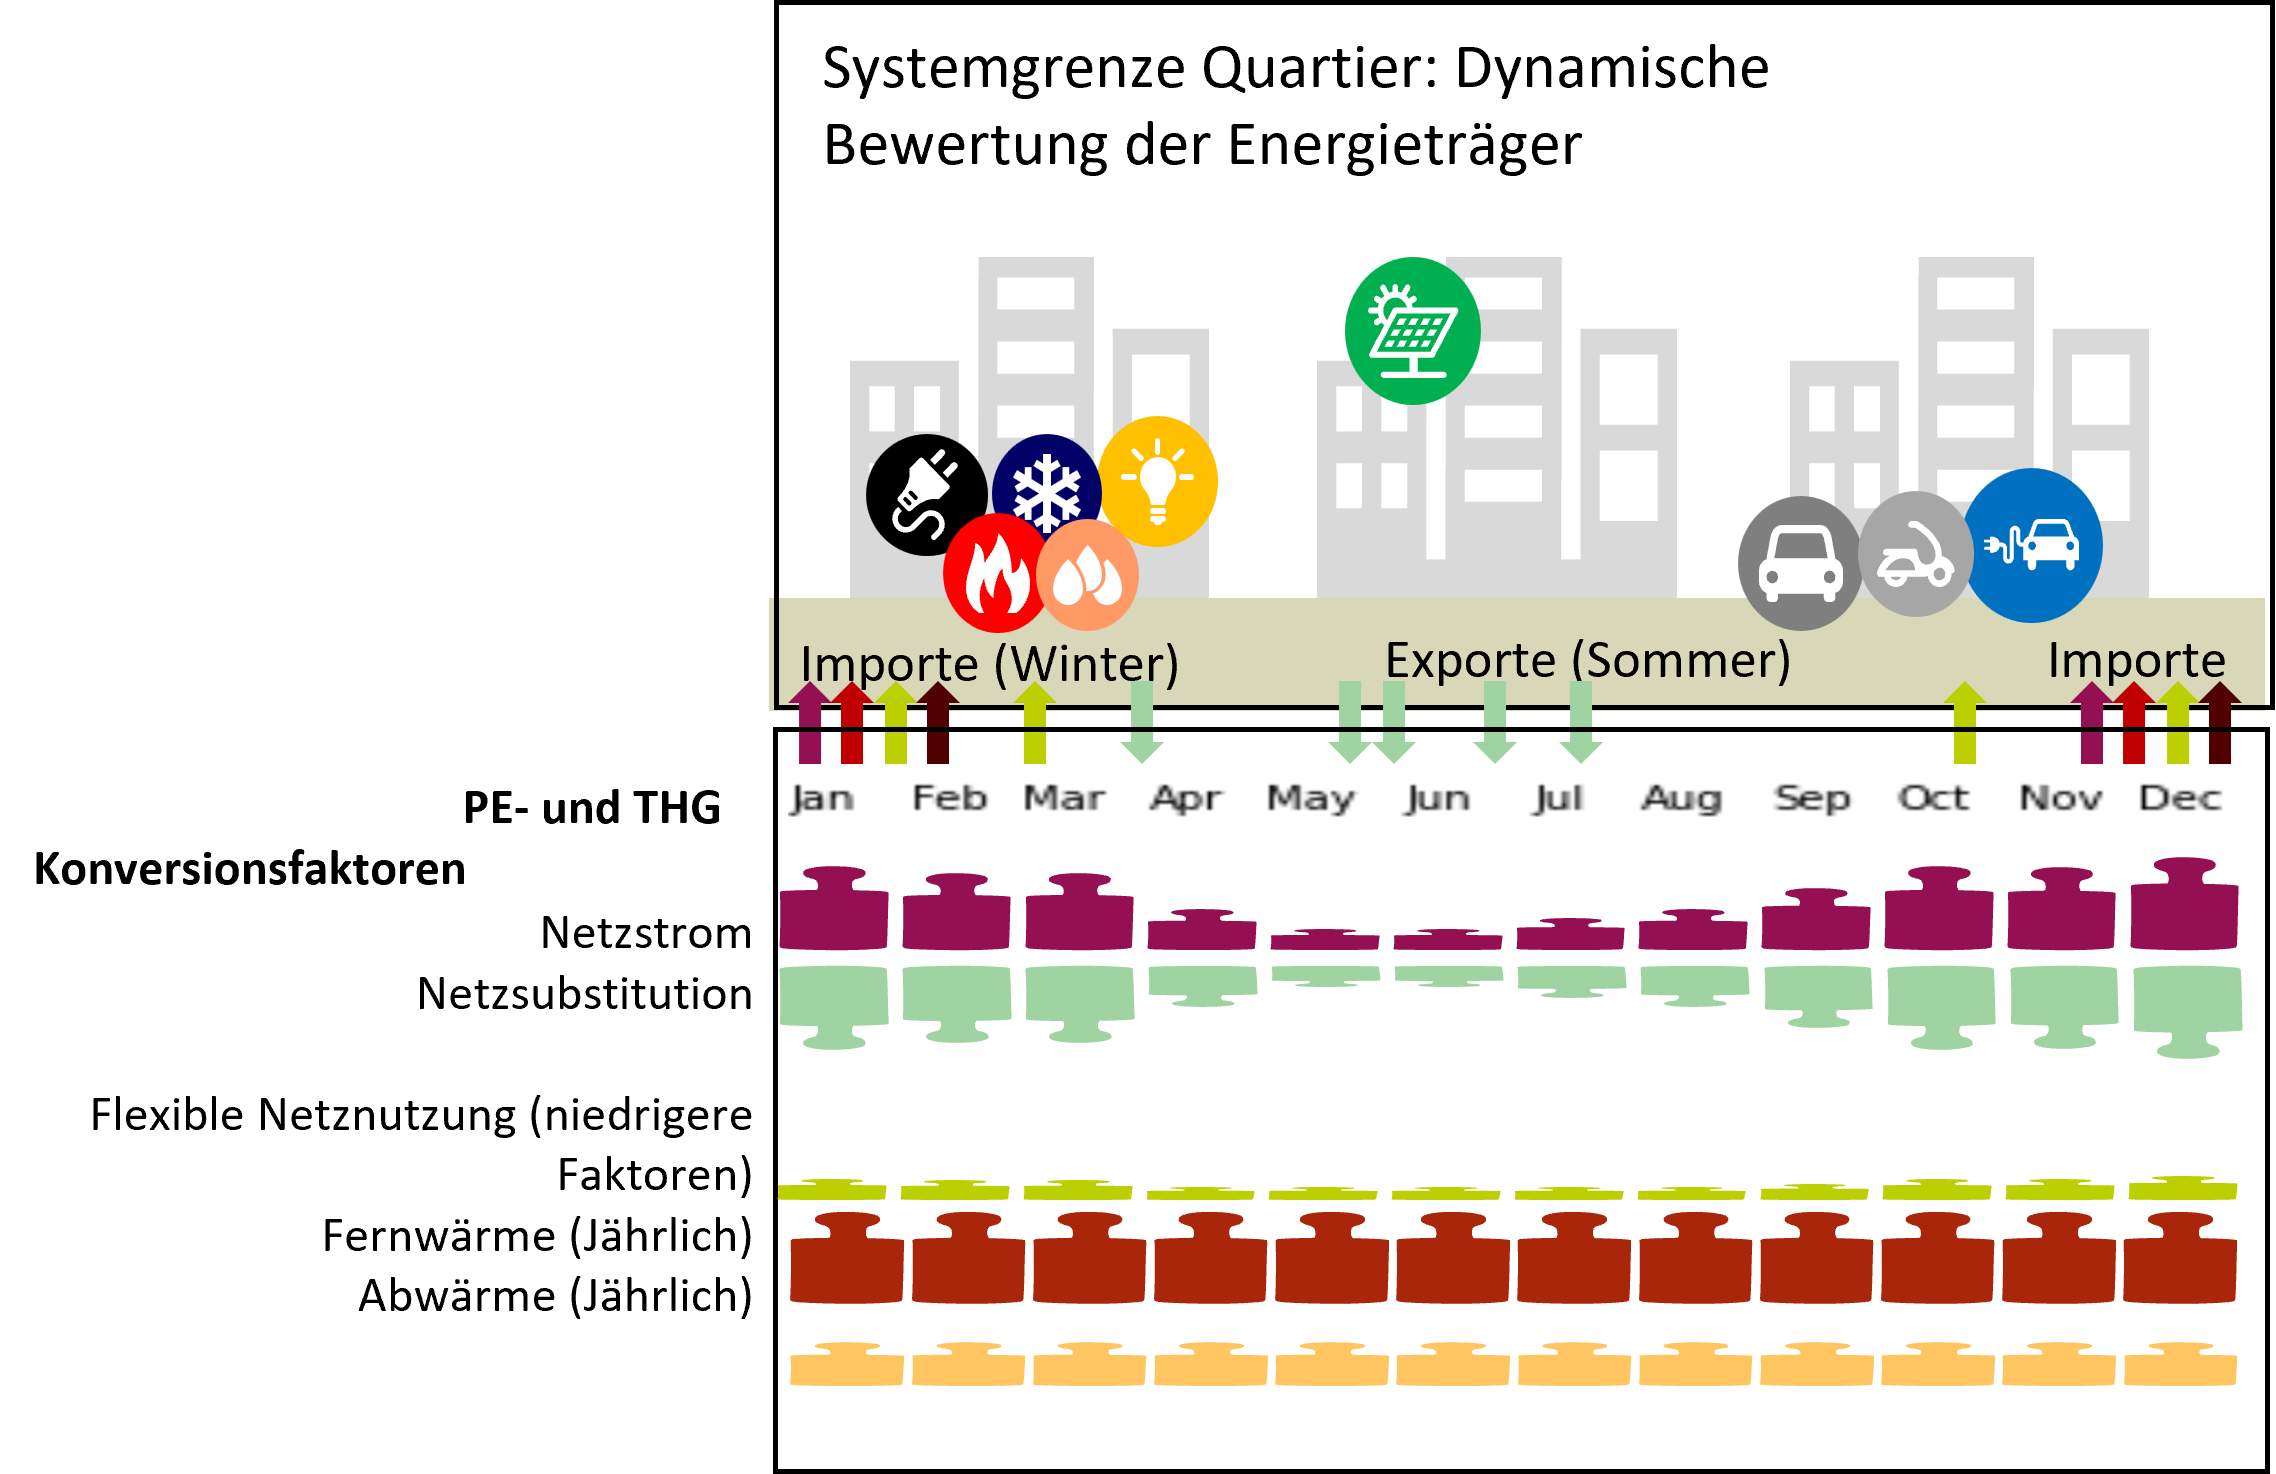
\includegraphics[width=0.9\linewidth,height=\textheight,keepaspectratio]{Kapitel/../Abbildungen/konversionsfaktoren_schema.png}

}

\caption{\label{fig-konversionsfaktoren}Abbildung -- Stundenflüsse und
monatliche Bewertung.}

\end{figure}%

\subsection{Bewertungszeitraum der
Treibhausgasbilanz}\label{bewertungszeitraum-der-treibhausgasbilanz}

Die Lebenszyklus-THG-Bilanz betrachtet den Zeitraum \textbf{2025--2075
(50 Jahre)}. Emissionen aus Errichtung, späteren Maßnahmen,
Gebäudebetrieb und Mobilität werden innerhalb dieses Zeitraums
kumuliert. Die Emissionsfaktoren folgen im Referenzverfahren
energieträger- und prozessbezogenen Entwicklungspfaden. Die angenommene
vollständige Dekarbonisierung der betrachteten Versorgung und Prozesse
\textbf{ab 2050} ist eine Szenarioannahme und kein Nachweis einer
bereits tatsächlich emissionsfreien Versorgung (Schneider u.~a. 2025,
Abschn. 2.4; Schneider 2026, Abschn. 3.2.8).

\section{Konsequenzen für die
Nachweisführung}\label{konsequenzen-fuxfcr-die-nachweisfuxfchrung}

Ein nachvollziehbarer Quartiersnachweis dokumentiert die
\textbf{Quartiersgrenze}, die \textbf{Bezugsflächen}, die
\textbf{Nutzungen}, die \textbf{zugeordneten Energie- und
Mobilitätsflüsse}, die \textbf{Lebenszyklusmodule} sowie die verwendeten
\textbf{Zeitreihen, Bewertungsfaktoren und Methodenstände}. Neben dem
Ergebnis nach Kontextkorrektur sollte die physische beziehungsweise
bewertete Bilanz \textbf{vor} Kontextfaktoren getrennt ausgewiesen
werden.

Die hier festgelegten Grenzen sind Teil des Bewertungsmaßstabs. Sie
ersetzen keine vertiefende bauphysikalische, anlagentechnische oder
gebäudebezogene Ökobilanz. Wie die Ergebnisse in Planung und Deklaration
zu verwenden sind, wird in Kapitel~\ref{sec-anwendung} beschrieben.

\chapter{Methodenstand und Fortschreibung}\label{sec-fortschreibung}

\begin{tcolorbox}[enhanced jigsaw, arc=.35mm, bottomrule=.15mm, breakable, colback=white, colframe=quarto-callout-note-color-frame, left=2mm, leftrule=.75mm, opacityback=0, rightrule=.15mm, toprule=.15mm]
\begin{minipage}[t]{5.5mm}
\textcolor{quarto-callout-note-color}{\faInfo}
\end{minipage}%
\begin{minipage}[t]{\textwidth - 5.5mm}

Arbeitsfassung vom 19. Oktober 2026

\end{minipage}%
\end{tcolorbox}

Einflussgrößen, Geltungsbereich und Regeln für die Fortschreibung

Der PEQ-Ansatz verbindet einen nationalen Bewertungsmaßstab mit dem
konkreten Quartierskonzept. Seine Aussagekraft hängt davon ab, dass
beide Seiten zusammenpassen: Das Budget muss zu den bilanzierten
Emissionen gehören, die Energieanforderung zum angenommenen
Versorgungssystem und die Simulation zum umsetzbaren Projekt. Eine
Fortschreibung überprüft deshalb Daten, Annahmen und Verteilungsregeln
gemeinsam.

\section{Was ein positives Ergebnis
aussagt}\label{was-ein-positives-ergebnis-aussagt}

Eine positive Primärenergiebilanz zeigt, dass das Quartier unter den
festgelegten Faktoren und Kontextregeln die energetische Anforderung
erfüllt. Die Klimaneutralitätsstufe verlangt zusätzlich die Einhaltung
des kumulierten THG-Budgets. Der Referenzwert von 320 kg CO₂e/m² BGF
setzt die L3-Senkenannahme und die beschriebenen Systemgrenzen voraus.
Er bedeutet weder Emissionsfreiheit am Standort noch einen vom Projekt
erbrachten Nachweis der national angenommenen Senkenleistung.

\section{Drei Arten von Änderungen}\label{drei-arten-von-uxe4nderungen}

Für einen nachvollziehbaren Methodenstand sind drei Ebenen zu
unterscheiden:

\begin{longtable}[]{@{}
  >{\raggedright\arraybackslash}p{(\linewidth - 4\tabcolsep) * \real{0.3333}}
  >{\raggedright\arraybackslash}p{(\linewidth - 4\tabcolsep) * \real{0.3333}}
  >{\raggedright\arraybackslash}p{(\linewidth - 4\tabcolsep) * \real{0.3333}}@{}}
\caption{Ebenen der
Fortschreibung.}\label{tbl-fortschreibung}\tabularnewline
\toprule\noalign{}
\begin{minipage}[b]{\linewidth}\raggedright
Ebene
\end{minipage} & \begin{minipage}[b]{\linewidth}\raggedright
Beispiel
\end{minipage} & \begin{minipage}[b]{\linewidth}\raggedright
Konsequenz
\end{minipage} \\
\midrule\noalign{}
\endfirsthead
\toprule\noalign{}
\begin{minipage}[b]{\linewidth}\raggedright
Ebene
\end{minipage} & \begin{minipage}[b]{\linewidth}\raggedright
Beispiel
\end{minipage} & \begin{minipage}[b]{\linewidth}\raggedright
Konsequenz
\end{minipage} \\
\midrule\noalign{}
\endhead
\bottomrule\noalign{}
\endlastfoot
Projektdaten & Geänderte PV-Fläche, andere Hülle, präzisierter
Wärmebedarf & Neues Ergebnis für das Projekt bei gleichem
Bewertungsmaßstab \\
Szenario und Parametrisierung & Neue Mobilitätsdaten, Emissionsfaktoren
oder Gebäudebestandsdaten & Geänderte Berechnungsgrundlage; bisherige
und neue Ergebnisse nur mit benanntem Stand vergleichen \\
Normative Verteilung & Anderer Sektoranteil, Sanierungskontext oder
Senkenansatz & Geänderter Bewertungsmaßstab mit eigener fachlicher
Begründung \\
\end{longtable}

Bei einer Neuauflage bleiben die zuvor verwendeten Faktoren und Annahmen
nachvollziehbar. Ob laufende oder abgeschlossene Deklarationen auf neue
Grundlagen umzustellen sind, ist eine eigene Verfahrensentscheidung. Aus
einer wissenschaftlichen Weiterentwicklung folgt nicht automatisch eine
rückwirkende Neubewertung.

\section{Einflussgrößen und Grenzen des
Modells}\label{einflussgruxf6uxdfen-und-grenzen-des-modells}

\subsection{Gebäudebestand und
Dichte}\label{gebuxe4udebestand-und-dichte}

Die Dichteanforderung hängt von der Verteilung der Gebäudequalitäten und
Flächen im nationalen Bestand ab. Neue Bestandsdaten ermöglichen eine
aktualisierte Kalibrierung. Dabei ist zuerst zu prüfen, welche Anteile
saniert, neu gebaut oder weiterbetrieben werden und welchen Beitrag
diese Gruppen leisten können. Die Anpassung einzelner Kurvenparameter
ohne diesen nationalen Zusammenhang würde die ursprüngliche
Lastenverteilung verändern, ohne ihre Wirkung zu erklären.

Eine aktualisierte Dichtekurve muss daher gemeinsam mit den zugrunde
gelegten Flächen, Nutzungen und Sanierungsszenarien dokumentiert werden.
Auch die Wirkung auf niedrige und hohe Dichten ist auszuweisen. Das
physikalische Grundprinzip bleibt davon unabhängig, wie in
Kapitel~\ref{sec-kontext-dichte} erläutert.

\subsection{Mobilität und zeitliche
Bewertungsfaktoren}\label{mobilituxe4t-und-zeitliche-bewertungsfaktoren}

Neue Mobilitätserhebungen können Wege, Verkehrsmittelwahl und
Standortunterschiede besser abbilden. Für eine Aktualisierung müssen
sowohl der zugeordnete Bedarf als auch die Verteilung des nationalen
Mobilitätsbudgets geprüft werden. Ein neues Fahrprofil allein begründet
noch keinen veränderten Budgetanspruch.

Bei den Energiefaktoren ist eine höhere zeitliche Auflösung fachlich
interessant, insbesondere für Speicher, gesteuertes Laden und externe
Flexibilität. Das Modell kann stündliche Faktoren verarbeiten. Ihr
Einsatz braucht jedoch geeignete, dokumentierte Daten und eine klare
Bedeutung der Faktoren. Die durchschnittliche Emissionsintensität eines
Strommixes und die durch zusätzlichen Verbrauch verursachte Änderung der
Erzeugung sind unterschiedliche Bewertungsansätze und dürfen nicht
unbegründet ausgetauscht werden.

Eine Fortschreibung sollte deshalb zunächst dieselben Projektvarianten
mit dem bisherigen und dem neuen Faktorsatz vergleichen. So wird
sichtbar, ob ein Ergebnis durch die technische Maßnahme oder durch den
geänderten Maßstab besser wird. Der Referenzansatz verwendet monatliche
Faktoren; stündliche Faktoren bilden eine gesonderte Bewertungsvariante
(Schneider 2026, Abschn. 3.2.3--3.2.4; Schneider u.~a. 2025, Abschn. 2.6
und 4.2--4.3).

\subsection{THG-Budget, PV und Senken}\label{thg-budget-pv-und-senken}

Beim THG-Budget bestimmen nationales Restbudget, Senkenannahme,
Sektoranteil und Bezugsfläche den verfügbaren Wert je Quadratmeter. Mehr
Bauaufgaben können eine Neuverteilung notwendig machen. Sie vergrößern
das Gesamtbudget jedoch nicht von selbst. Jede zusätzliche Zuteilung ist
deshalb mit ihrer Deckung oder der damit verbundenen Änderung des
Klimaziels zu begründen.

Für die PV-Abgrenzung ist eine konsistente Alternative mit Einbeziehung
der Errichtungsemissionen auf Quartiersebene zu untersuchen. Dabei
werden die zugehörigen Emissionen und Budgetanteile aus dem
Energieversorgungssektor entsprechend zugeordnet. Die Untersuchung
sollte zeigen, wie sich Grenzwert, Quartiersbilanz und Anreiz zum
PV-Ausbau gemeinsam verändern. Das ist eine methodische
Weiterentwicklung und keine bloße Ergänzung einer fehlenden
Bauteilposition.

Senken bleiben eine besonders wirksame Annahme. Eine weniger günstige
Senkenentwicklung verkleinert den Spielraum für Emissionen. Die
Varianten L1 bis L3 machen diese Abhängigkeit sichtbar. Für robuste
Planung lohnt es sich daher, neben dem Erfüllen des Referenzwerts auch
den Abstand zu den strengeren Varianten zu kennen (Schneider u.~a. 2025,
Abschn. 2.3 und 4.2--4.3).

\subsection{Sanierung und bauliche
Absenkpfade}\label{sanierung-und-bauliche-absenkpfade}

Der Entwurf differenziert die Sanierungsanpassung nach energetischer
Typologie und baulichen Randbedingungen. Dafür braucht es eine
belastbare Datengrundlage und eine Regel, die in der Planung mit
vertretbarem Aufwand nachweisbar ist. Eine kleinteilige Differenzierung
wäre wenig hilfreich, wenn die erforderlichen Informationen erst spät
oder nur mit unverhältnismäßigem Aufwand verfügbar sind.

Für Renovierungsfahrpläne sind außerdem die Herstellungsemissionen zum
Maßnahmenzeitpunkt von Bauteilen relevant. Europäische Arbeiten zur
Lebenszyklusbewertung liefern dafür Szenarien und Vergleichsgrundlagen.
Die EU-Roadmap verbindet Gebäude- und Bestandsmodelle mit Maßnahmen an
Materialproduktion, Materialeinsatz und Bautätigkeit (Le Den u.~a.
2024). Die INDICATE-Arbeiten zeigen ergänzend, wie nationale
Ausgangswerte mit einheitlichen Erhebungsgrundlagen aufgebaut werden
können und warum Unterschiede der Bilanzmethoden den Vergleich
erschweren (BPIE 2024). Daraus lassen sich Prüfaufgaben für die
Fortschreibung ableiten; konkrete österreichische Materialpfade müssen
gesondert ausgewählt und auf den PEQ-Bilanzumfang abgestimmt werden.

\section{Kommunale Allokation als zusätzliche
Ebene}\label{kommunale-allokation-als-zusuxe4tzliche-ebene}

Eine kommunale Allokation könnte nationale Vorgaben zunächst auf eine
Stadt oder Gemeinde und anschließend auf ihre Quartiere beziehen. Für
eine Stadt wie Wien wären dabei etwa Gebäudebestand, erwartete
Flächenentwicklung, Energieinfrastruktur und Mobilitätsstruktur
gemeinsam zu betrachten. Diese Ebene ist als Erweiterung angelegt und
bislang kein eigener implementierter Kontextfaktor (Schneider 2026,
Abschn. 3.5.1, S. 89--90).

Eine Kommune könnte damit verdeutlichen, welche Beiträge sie aus
Bestandssanierung, Neubau und Infrastruktur erwartet. Voraussetzung ist
eine konsistente Verschachtelung: Ein bereits national oder kommunal
zugeteiltes Budget darf nicht mehrfach als zusätzliche Entlastung auf
Quartiersebene erscheinen. Unterschiedliche lokale Ausgangslagen sind
begründbar zu berücksichtigen, ohne die Gesamtmenge aus dem Blick zu
verlieren.

\section{Lernen aus Planung und
Betrieb}\label{lernen-aus-planung-und-betrieb}

Die weitere Absicherung des Verfahrens braucht neben neuen Szenarien
auch Erfahrungen aus realisierten Projekten. Ein Abgleich mit
Betriebsdaten kann zeigen, ob Bedarfsprofile, Regelung und
Speicherbetrieb die vorgesehenen Beiträge erbringen. Abweichungen sind
zunächst auf Nutzung, Wetter, Ausführung und Betrieb zu untersuchen,
bevor daraus eine Änderung des Bewertungsmaßstabs abgeleitet wird.

\part{Anwendung}

\chapter{Deklaration von Bauprojekten}\label{sec-anwendung}

Vom untersuchten Konzept über die realisierte Lösung bis zum
nachgewiesenen Betrieb

Der klimaaktiv Standard kann in unterschiedlichen Projektphasen
angewendet werden. Dabei sind zwei Fragen zu unterscheiden:
\textbf{Welche Qualitätsstufe wird rechnerisch erreicht?} Und
\textbf{wie belastbar ist der zugrunde liegende Projektstand?} Die
Qualitätsstufen beschreibt \hyperref[sec-standard]{Der Standard}; die
Deklarationsphase kennzeichnet den Stand der Nachweisführung.

\section{Drei Deklarationsphasen}\label{drei-deklarationsphasen}

Die Nachweisführung kann in der Planung, nach Fertigstellung sowie auf
Grundlage gemessener Betriebsdaten erfolgen. Mit fortschreitendem
Projektstand verändert sich die Datengrundlage und damit die
Aussagekraft der Deklaration.

\begin{figure}

\centering{

\includegraphics[width=1\linewidth,height=\textheight,keepaspectratio]{index_files/mediabag/Kapitel/../Abbildungen/deklarationen.pdf}

}

\caption{\label{fig-deklarationsphasen}\textbf{Deklaration je nach
Projektstand:} Planungsdeklaration, Fertigstellungsdeklaration und
Betriebsdeklaration mit zunehmender Verfügbarkeit von Ausführungs- und
Messdaten.}

\end{figure}%

\subsection{📐 Planungsdeklaration -- Potenziale und Varianten
nachweisen}\label{planungsdeklaration-potenziale-und-varianten-nachweisen}

Eine \textbf{Planungsdeklaration} zeichnet die fundierte Untersuchung
eines Quartierskonzepts aus. Sie zeigt, \textbf{unter welchen
planerischen, technischen und organisatorischen Voraussetzungen} eine
angestrebte Qualitätsstufe erreicht werden könnte. Insbesondere in
frühen Phasen ermöglicht sie die Beantwortung von
\emph{Was-wäre-wenn-Fragen}: Welche PV-Flächen wären erforderlich?
Welche Wärmeversorgung oder Mobilitätsmaßnahmen würden den Ausschlag
geben? Wie stark beeinflussen unterschiedliche Bauweisen die THG-Bilanz?

Die betrachtete Variante \textbf{muss nicht später genau so umgesetzt
werden}. Eine Planungsdeklaration ist daher weder eine
Ausführungsverpflichtung noch ein Nachweis der später tatsächlich
erreichten Performance. Entscheidend sind eine ausreichend detaillierte,
nachvollziehbare Untersuchung sowie die transparente Kennzeichnung der
zugrunde liegenden Annahmen und Abhängigkeiten.

\subsection{🏗️ Fertigstellungsdeklaration -- Umsetzung
überprüfen}\label{fertigstellungsdeklaration-umsetzung-uxfcberpruxfcfen}

Die \textbf{Fertigstellungsdeklaration} bewertet das \textbf{tatsächlich
errichtete beziehungsweise sanierte Quartier}. Die in der Planung
angesetzten Maßnahmen werden mit dem Ausführungsstand abgeglichen: etwa
Gebäudehülle, installierte Wärmeerzeugung, tatsächlich verfügbare
PV-Flächen und -Leistungen, Speicher, Ladeinfrastruktur sowie
realisierte Mobilitätsangebote.

Abweichungen von früheren Varianten sind zu dokumentieren und, soweit
bilanzrelevant, neu zu bewerten. Maßgeblich ist die nachvollziehbar
belegte Ausführung und die daraus berechnete Zielerreichung -- nicht
allein das ursprüngliche Planungsergebnis.

\subsection{🔍 Betriebs- bzw. Monitoringdeklaration -- Wirkung im
Betrieb
belegen}\label{betriebs--bzw.-monitoringdeklaration-wirkung-im-betrieb-belegen}

Die \textbf{Betriebsdeklaration} ergänzt die modellbasierte Bewertung um
\textbf{gemessene Betriebsdaten} aus einer mindestens einjährigen
Monitoringphase. Insbesondere Energiebezug, Erzeugung und Einspeisung
sowie -- soweit erfassbar und für die gewählte Qualitätsstufe relevant
-- weitere Energieflüsse und Nutzungsbedingungen werden mit den Annahmen
der Bewertung abgeglichen.

Eine sachgerechte Interpretation berücksichtigt unter anderem Wetter,
Belegung, Nutzungsänderungen und die Verfügbarkeit der technischen
Anlagen. Das Monitoring ermöglicht es, Abweichungen zwischen
prognostizierter und tatsächlicher Performance zu erkennen. Es ersetzt
jedoch nicht die Bilanzierung jener Lebenszyklus- oder
Mobilitätsemissionen, die nicht unmittelbar gemessen werden können.

\begin{longtable}[]{@{}
  >{\raggedright\arraybackslash}p{(\linewidth - 4\tabcolsep) * \real{0.3333}}
  >{\raggedright\arraybackslash}p{(\linewidth - 4\tabcolsep) * \real{0.3333}}
  >{\raggedright\arraybackslash}p{(\linewidth - 4\tabcolsep) * \real{0.3333}}@{}}
\caption{Bewertungsgrundlagen und Aussagekraft der
Deklarationsphasen.}\label{tbl-deklarationsphasen}\tabularnewline
\toprule\noalign{}
\begin{minipage}[b]{\linewidth}\raggedright
Phase
\end{minipage} & \begin{minipage}[b]{\linewidth}\raggedright
Bewertungsgrundlage
\end{minipage} & \begin{minipage}[b]{\linewidth}\raggedright
Aussage der Deklaration
\end{minipage} \\
\midrule\noalign{}
\endfirsthead
\toprule\noalign{}
\begin{minipage}[b]{\linewidth}\raggedright
Phase
\end{minipage} & \begin{minipage}[b]{\linewidth}\raggedright
Bewertungsgrundlage
\end{minipage} & \begin{minipage}[b]{\linewidth}\raggedright
Aussage der Deklaration
\end{minipage} \\
\midrule\noalign{}
\endhead
\bottomrule\noalign{}
\endlastfoot
📐 \textbf{Planung} & Quartierskonzept, Fachannahmen und untersuchte
Varianten & Unter welchen Bedingungen eine Qualitätsstufe erreichbar
ist \\
🏗️ \textbf{Fertigstellung} & Nachgewiesene Ausführung und aktualisierte
Berechnung & Ob das ausgeführte Projekt die Anforderungen erfüllt \\
🔍 \textbf{Betrieb / Monitoring} & Messdaten und dokumentierte
Betriebsbedingungen & Inwieweit die prognostizierte Performance im
Betrieb bestätigt wird \\
\end{longtable}

\begin{tcolorbox}[enhanced jigsaw, arc=.35mm, bottomrule=.15mm, breakable, colback=white, colframe=quarto-callout-warning-color-frame, left=2mm, leftrule=.75mm, opacityback=0, rightrule=.15mm, toprule=.15mm]
\begin{minipage}[t]{5.5mm}
\textcolor{quarto-callout-warning-color}{\faExclamationTriangle}
\end{minipage}%
\begin{minipage}[t]{\textwidth - 5.5mm}

\vspace{-3mm}\textbf{Qualitätsstufe ist nicht Deklarationsphase}\vspace{3mm}

Die \textbf{Qualitätsstufe} bezeichnet den Umfang der erfüllten Energie-
und THG-Anforderungen. Die \textbf{Deklarationsphase} beschreibt, ob die
Beurteilung auf Planungsannahmen, der realisierten Ausführung oder
gemessenen Betriebsdaten beruht. Beide Angaben sind unabhängig
voneinander und müssen gemeinsam ausgewiesen werden.

\end{minipage}%
\end{tcolorbox}

\section{🧭 „Auf dem Weg`` -- Zielerreichung in
Etappen}\label{auf-dem-weg-zielerreichung-in-etappen}

Nicht jedes Quartier erfüllt bereits \textbf{zum Nachweiszeitpunkt}
sämtliche Anforderungen einer angestrebten Qualitätsstufe. Vor allem im
Bestand oder bei abschnittsweiser Entwicklung können wesentliche
Maßnahmen erst später wirksam werden.

Die Deklaration \textbf{„Auf dem Weg zum Plus-Energie-Quartier``}
berücksichtigt solche Entwicklungspfade, sofern eine spätere
Zielerreichung innerhalb des vorgesehenen Zeitraums plausibel
nachgewiesen werden kann. Das Konzept sieht hierfür einen Zeitraum von
bis zu fünf Jahren vor.

Entscheidend ist die Unterscheidung zwischen einer allgemeinen Absicht
und einem \textbf{technisch sowie zeitlich glaubhaften Umsetzungspfad}.
Geeignete Nachweise können insbesondere sein:

\begin{itemize}
\tightlist
\item
  \textbf{PV-Vorhalteflächen:} planerisch gesicherte Dach- oder
  Fassadenflächen einschließlich Tragfähigkeit, Verschattung,
  Leitungsführung und geplanter Anschlussmöglichkeit.
\item
  \textbf{Vorbereitete Energieflexibilität:} Mess-, Steuer- und
  Kommunikationsinfrastruktur sowie ein umsetzbares Regelungskonzept.
\item
  \textbf{Technische Vorhaltungen:} Leerrohre, Platzreserven, Trassen
  oder elektrische Anschlussreserven für einen späteren Ausbau.
\item
  \textbf{Nachvollziehbare Etappen:} konkrete Maßnahmen,
  Verantwortlichkeiten, Voraussetzungen und Zeitpunkte der Umsetzung.
\end{itemize}

Ein solcher Pfad ist \textbf{kein Nachweis einer bereits erreichten
Qualitätsstufe}. Der aktuelle Zustand und die angestrebte vollständige
Zielerreichung müssen getrennt dargestellt werden.

Für die THG-Bewertung sind außerdem die Emissionen bis zur späteren
Umsetzung und die zusätzlichen Herstellungsemissionen der Maßnahmen zu
berücksichtigen. Ein gutes Ergebnis im Zieljahr macht bereits
entstandene Emissionen nicht rückgängig.

Die vertiefte Darstellung von Renovierungsetappen findet sich unter
\href{07-renovierungsfahrplan.qmd}{Sanierungsfahrpläne}.

\begin{tcolorbox}[enhanced jigsaw, arc=.35mm, bottomrule=.15mm, breakable, colback=white, colframe=quarto-callout-note-color-frame, left=2mm, leftrule=.75mm, opacityback=0, rightrule=.15mm, toprule=.15mm]

\vspace{-3mm}\textbf{Methodische Einordnung}\vspace{3mm}

Die verbindlichen Bedingungen für eine Deklaration „Auf dem Weg``,
insbesondere Fristen, erforderliche Nachweise und die Zuordnung zur
Qualitätsstufe, richten sich nach den jeweils gültigen
Deklarationsvorgaben.

\end{tcolorbox}

\section{Ablauf der
Nachweisführung}\label{ablauf-der-nachweisfuxfchrung}

Der Weg zur klimaaktiv Auszeichnung wird durch ein Netzwerk aus
Anlaufstelle, Kompetenzpartner:innen und Expert:innengremium begleitet.
Der Ablauf lässt sich aus Sicht der Projektverantwortlichen in drei
Schritte gliedern.

\begin{figure}

\centering{

\includegraphics[width=1\linewidth,height=\textheight,keepaspectratio]{index_files/mediabag/Kapitel/../Abbildungen/ihr_weg_zum_peq.pdf}

}

\caption{\label{fig-weg-zum-peq}\textbf{Ihr Weg zum
Plus-Energie-Quartier:} Von der ersten Prüfung der Mindestanforderungen
über die Auswahl einer fachlichen Projektbegleitung bis zur Einreichung
und Qualitätssicherung.}

\end{figure}%

\subsection{Schritt 1 -- Mindestanforderungen und Aussichten
prüfen}\label{schritt-1-mindestanforderungen-und-aussichten-pruxfcfen}

Zu Beginn werden die grundsätzlichen Voraussetzungen des Vorhabens und
die Aussichten auf eine erfolgreiche Deklaration geklärt. Ein
\textbf{PEQ-Quick-Check} kann eine erste Einschätzung ermöglichen.

Dabei werden mögliche Anpassungen des Projektkonzepts, offene
Anforderungen und ein geeigneter Zeitplan besprochen. Für diese erste
Orientierung steht die \textbf{Anlaufstelle Plus-Energie-Quartiere} zur
Verfügung.

\subsection{Schritt 2 -- Kompetenzpartner:in
auswählen}\label{schritt-2-kompetenzpartnerin-auswuxe4hlen}

Für die vertiefte Bearbeitung können Projektverantwortliche eine:n
\textbf{klimaaktiv Kompetenzpartner:in} auswählen.

Gemeinsam werden der Projektumfang, die Bilanzgrenzen, die untersuchten
Varianten und der Leistungsumfang der Begleitung festgelegt. Dazu
gehören gegebenenfalls die Datenerhebung, Berechnung, fachliche Beratung
und Vorbereitung der Deklarationsunterlagen.

Die Kompetenzpartner:innen unterstützen die Anwendung des Standards und
die nachvollziehbare Aufbereitung der erforderlichen Nachweise.

\subsection{Schritt 3 -- Einreichung und
Qualitätssicherung}\label{schritt-3-einreichung-und-qualituxe4tssicherung}

Nach Abschluss der Projektbegleitung werden die erforderlichen
Ergebnisse und Unterlagen zur fachlichen Prüfung übermittelt.

Das \textbf{klimaaktiv Expert:innengremium} prüft die Nachweisführung
und kann Rückfragen zu einzelnen Annahmen, Berechnungen oder Belegen
stellen. Nach erfolgreicher Prüfung erfolgt die entsprechende
Deklaration beziehungsweise Auszeichnung.

Die Qualitätssicherung dient insbesondere der fachlichen
Plausibilisierung, Nachvollziehbarkeit und einheitlichen Anwendung des
Standards.

\section{Akteure und
Zuständigkeiten}\label{akteure-und-zustuxe4ndigkeiten}

Die Nachweisführung ist in die Organisationsstruktur des klimaaktiv
Programms für Siedlungen und Quartiere eingebettet. Die beteiligten
Akteure übernehmen unterschiedliche, aufeinander abgestimmte Aufgaben.

\begin{figure}

\centering{

\includegraphics[width=1\linewidth,height=\textheight,keepaspectratio]{index_files/mediabag/Kapitel/../Abbildungen/programmteam.pdf}

}

\caption{\label{fig-programmteam}\textbf{Das klimaaktiv Programmteam:}
Anlaufstelle, Siedlungen-und-Quartiere-Team, Kompetenzpartner:innen und
Expert:innengremium sowie ihre Zusammenarbeit mit
Projektverantwortlichen und Fachplanenden.}

\end{figure}%

Die wesentlichen Rollen sind:

\begin{itemize}
\tightlist
\item
  \textbf{Anlaufstelle Plus-Energie-Quartiere:} Erstinformation,
  Beratung zur grundsätzlichen Anwendbarkeit des Standards und
  Unterstützung bei Fragen zur Nachweisführung.
\item
  \textbf{klimaaktiv Siedlungen und Quartiere:} Programmkoordination und
  Unterstützung der entsprechenden Qualitätssicherungs- und
  Beratungsstrukturen.
\item
  \textbf{klimaaktiv Kompetenzpartner:innen:} Projektbezogene Beratung,
  Bewertung und Unterstützung bei der Erarbeitung der
  Nachweisunterlagen.
\item
  \textbf{klimaaktiv Expert:innengremium:} Fachliche Qualitätssicherung
  und Prüfung der eingereichten Ergebnisse.
\item
  \textbf{Projektverantwortliche und Fachplanende:} Erarbeitung des
  Projekts, Bereitstellung der notwendigen Daten, Umsetzung der
  Maßnahmen und Dokumentation der Nachweise.
\end{itemize}

Die Zusammenarbeit zwischen den beteiligten Stellen soll eine
nachvollziehbare Bewertung ermöglichen, ohne die Verantwortlichkeiten
für Projektplanung, Berechnung und Qualitätssicherung zu vermischen.

\section{Anforderungen an Datenqualität und
Nachvollziehbarkeit}\label{anforderungen-an-datenqualituxe4t-und-nachvollziehbarkeit}

Die Nachweisführung bündelt Angaben aus Architektur, Bauphysik,
Haustechnik, Mobilitätsplanung und Ökobilanz. Für ergebnisrelevante
Eingaben ist zu kennzeichnen, ob es sich um \textbf{Referenzannahmen},
\textbf{projektspezifische Berechnungen}, \textbf{bestätigte
Ausführungsangaben} oder \textbf{Messwerte} handelt. Abhängigkeiten von
nicht gesicherten Maßnahmen sind sichtbar auszuweisen.

Für Variantenvergleiche sind Quartiersabgrenzung, Nutzungsumfang,
Flächenbezüge und Bewertungsstand konsistent zu halten. Werden sie
verändert, muss die Auswirkung auf Bedarf, Kontextfaktoren und
zugeteilte Budgets kenntlich gemacht werden. Die Interpretation der
Ergebnisse wird unter Kapitel~\ref{sec-ergebnisse} erläutert.

\section{\texorpdfstring{\href{../Abbildungen/logo.svg}{} PEExcel als
Nachweiswerkzeug}{ PEExcel als Nachweiswerkzeug}}\label{peexcel-als-nachweiswerkzeug}

Die Berechnungen und Variantenvergleiche werden mit dem
\href{https://simonschaluppe.github.io/peexcel/}{PEExcel-Nachweistool}
unterstützt. \textbf{Bedienung, Datenmodell, Auswertungsfunktionen,
Softwareversionen und technische Modellimplementierung} sind auf der
eigenständigen Toolwebsite beschrieben.

Dieser Bericht erläutert die Bewertungsgrundlagen
(Kapitel~\ref{sec-allokation}, Kapitel~\ref{sec-kontext},
Kapitel~\ref{sec-bilanzregeln}) und ihre Interpretation
(Kapitel~\ref{sec-ergebnisse}); er ersetzt keine detaillierte
Fachplanung.

\begin{tcolorbox}[enhanced jigsaw, arc=.35mm, bottomrule=.15mm, breakable, colback=white, colframe=quarto-callout-tip-color-frame, left=2mm, leftrule=.75mm, opacityback=0, rightrule=.15mm, toprule=.15mm]

\vspace{-3mm}\textbf{Weiterführende Informationen}\vspace{3mm}

\href{https://simonschaluppe.github.io/peexcel/}{PEExcel
Wissensplattform} · \href{07-ergebnisse.qmd}{Ergebnisinterpretation} ·
\href{07-praxisbeispiele.qmd}{Praxisbeispiele} ·
\href{07-renovierungsfahrplan.qmd}{Sanierungsfahrpläne}

\end{tcolorbox}

\chapter{Ergebnisse verstehen}\label{sec-ergebnisse}

Von der Zielerreichung zur nachvollziehbaren Planungsentscheidung

Die erreichte Qualitätsstufe fasst die Bewertung zusammen. Für die
Planung ist ebenso wichtig, \textbf{welche realen Energie- und
Emissionsflüsse, Kontextfaktoren und Annahmen} dahinterstehen. Eine
nachvollziehbare Ergebnisdarstellung zeigt deshalb die einzelnen
Beiträge und nicht nur „bestanden`` oder „nicht bestanden``.

\section{Primärenergiebilanz}\label{primuxe4renergiebilanz}

Der berechnete Energiebedarf, die lokale Erzeugung sowie Bezug und
Export über die Quartiersgrenze sind \textbf{physische Größen}. Erst die
Gewichtung ergibt den Primärenergiesaldo. Dichte-, Mobilitäts- und
Sanierungskontext verändern den Bewertungsmaßstab, nicht den realen
Energiefluss. Die zugrunde liegenden Regeln erläutern
Kapitel~\ref{sec-bilanzregeln} und Kapitel~\ref{sec-kontext}.

Eine positive Bewertungsbilanz ist nicht gleichbedeutend mit Autarkie
oder einem physischen Nettoexport. Für aussagekräftige Vergleiche sind
Rohsaldo und jede Kontextkorrektur getrennt auszuweisen.

Die Ergebnisdarstellung stellt Energiebedarf und Energieaufbringung
gegenüber und weist die Kontextkomponenten gesondert aus. Die
Erweiterung um Mobilität verändert sowohl die bilanzierten Bedarfe als
auch die zugerechneten Budgets.

\begin{tcolorbox}[enhanced jigsaw, arc=.35mm, bottomrule=.15mm, breakable, colback=white, colframe=quarto-callout-note-color-frame, left=2mm, leftrule=.75mm, opacityback=0, rightrule=.15mm, toprule=.15mm]

\vspace{-3mm}\textbf{Abbildungsvorschlag E2 · Bilanzzerlegung (Plotly)}\vspace{3mm}

\textbf{Interaktives Diagramm:} Energiebilanz vor Kontext →
Dichtegutschrift/-lastschrift → Mobilitätsbudget → Sanierungsgutschrift
→ bewerteter Saldo. Tooltips mit Definition, Einheit, Vorzeichen und
Quelle. Für PDF eine statische Fassung vorsehen.

\end{tcolorbox}

\begin{figure}

\centering{

\includegraphics[width=0.95\linewidth,height=\textheight,keepaspectratio]{index_files/mediabag/Kapitel/../Abbildungen/energiebilanz_erklaert.pdf}

}

\caption{\label{fig-energiebilanz-erklaert}Exemplarische
Primärenergiebilanzen eines Plus-Energie-Quartiers mit und ohne
Berücksichtigung der Mobilität.}

\end{figure}%

\section{Treibhausgasbudget und zeitlicher
Verlauf}\label{treibhausgasbudget-und-zeitlicher-verlauf}

Die THG-Bewertung der dritten Qualitätsstufe umfasst die im Standard
festgelegten baulichen, betrieblichen und mobilitätsbezogenen
Emissionen. Die kumulierte Bilanz wird dem zugeteilten Budget
gegenübergestellt. \textbf{Zeitpunkt und Art der Emissionen} sind für
die Interpretation wesentlich: Herstellungsemissionen entstehen bei der
baulichen Maßnahme, während Betriebsemissionen über die Jahre anfallen.

Das für den dokumentierten Methodenstand verwendete Referenzbudget und
seine Annahmen werden in Kapitel~\ref{sec-zielwert-thg} erläutert; die
Systemgrenzen stehen in Kapitel~\ref{sec-bilanzregeln}.

Die kumulierte THG-Bilanz setzt sich aus den einzelnen baulichen,
betrieblichen und mobilitätsbezogenen Emissionsbeiträgen zusammen. Die
Gegenüberstellung mit dem Budget zeigt den verbleibenden Spielraum
beziehungsweise eine Überschreitung.

\begin{figure}

\centering{

\includegraphics[width=0.95\linewidth,height=\textheight,keepaspectratio]{index_files/mediabag/Kapitel/../Abbildungen/emissionsbilanz_erklaert.pdf}

}

\caption{\label{fig-emissionsbilanz-erklaert}Beispielhafte
Zusammensetzung der kumulierten Lebenszyklus-Treibhausgasbilanz und
Vergleich mit dem Budget von 320 kg CO₂e/m² BGF.}

\end{figure}%

\chapter{Praxisbeispiele}\label{sec-praxisbeispiele}

Was die Bewertungsregeln für unterschiedliche Quartiere bedeuten

\begin{figure}

\centering{

\includegraphics[width=1\linewidth,height=\textheight,keepaspectratio]{index_files/mediabag/Kapitel/../Abbildungen/beispiele.pdf}

}

\caption{\label{fig-quartierstypologien-vergleich}Vergleich
exemplarischer Quartierstypologien anhand ihrer Primärenergiebedarfe,
Energieaufbringung und Kontextkomponenten.}

\end{figure}%

Die Beispiele illustrieren unterschiedliche Planungsaufgaben: Die
zusätzliche Anforderung an ein Neubau-Quartier mit niedriger baulicher
Dichte, die Herausforderungen im Kontext des hochverdichteten gemischten
Neubaus und die energetische Sanierung eines bestehenden Wohnquartiers.

\section{Am Bichl III -- Dichte als zusätzliche
Anforderung}\label{am-bichl-iii-dichte-als-zusuxe4tzliche-anforderung}

Am Bichl III wurde im Oktober 2026 als erstes Quartier in Österreich die
\texttt{🏗️\ Fertigsstellungsdeklaration\ Plus-Energie-Quartier}
verliehen. Der hier dokumentierte Deklarationsumfang umfasst die
Betriebsenergie.

Das Beispiel verdeutlicht die Wirkung des Dichtekontexts: Bei geringer
baulicher Dichte wird ein zusätzlicher energetischer Beitrag verlangt.
Im Fall von Am Bichl III konnte diese Anforderung durch die vorgesehene
Flexibilität beim Heizen und Kühlen kompensiert werden.

\section{RUGInnovation -- Sanierung und integrierte
Energieversorgung}\label{ruginnovation-sanierung-und-integrierte-energieversorgung}

Das Wiener Projekt RUGInnovation kombiniert die Sanierung einer
Wohnanlage mit einer veränderten Energieversorgung und Photovoltaik auf
Dach- und Fassadenflächen. Dokumentiert sind unter anderem Arbeiten an
Fassade, Dach und Fenstern, eine Grundwasserwärmepumpe sowie
Mobilitätsmaßnahmen (Schneider u.~a. 2026, 15--19).

Der Fall zeigt, wie Gebäudehülle, Wärmeversorgung, erneuerbare Erzeugung
und Mobilität gemeinsam wirken. Die Sanierungsgutschrift entschärft die
energetische Anforderung; tatsächliche Einsparungen entstehen dagegen
durch die umgesetzten Maßnahmen. Deshalb sollten zunächst
Betriebsenergie, danach die Erweiterung um Mobilität und schließlich die
baulichen THG-Beiträge getrennt betrachtet werden.

\begin{tcolorbox}[enhanced jigsaw, arc=.35mm, bottomrule=.15mm, breakable, colback=white, colframe=quarto-callout-note-color-frame, left=2mm, leftrule=.75mm, opacityback=0, rightrule=.15mm, toprule=.15mm]

\vspace{-3mm}\textbf{Abbildungsvorschlag P2 · RUGInnovation -- drei Bilanzebenen}\vspace{3mm}

\textbf{Plotly:} Betriebsenergie → inklusive MIV →
THG-Lebenszyklusbewertung. Einmal mit tatsächlichem Datenstand und
geeigneten Anmerkungen zu Sanierung, PV, Wärmeversorgung und Budget; für
PDF statischer Export. Die drei Stufen nur zeigen, soweit dafür
freigegebene Berechnungen vorliegen.

\end{tcolorbox}

\chapter{Sanierungsfahrpläne und
Entwicklungspfade}\label{sec-renovierungsfahrplan}

„Auf dem Weg`` zum klimaneutralen Plus-Energie-Quartier

Bestandsquartiere werden häufig schrittweise saniert. Ein
Renovierungsfahrplan kann deshalb mit einer Folge von
Quartiersbewertungen verbunden werden. Die Darstellung zeigt den
erwarteten Zustand nach jeder Etappe, die noch erforderlichen Maßnahmen
und die bis dahin verursachten Emissionen.

\begin{tcolorbox}[enhanced jigsaw, arc=.35mm, bottomrule=.15mm, breakable, colback=white, colframe=quarto-callout-warning-color-frame, left=2mm, leftrule=.75mm, opacityback=0, rightrule=.15mm, toprule=.15mm]

\vspace{-3mm}\textbf{Entwicklungsperspektive -- keine zusätzliche Deklarationsstufe}\vspace{3mm}

Der hier beschriebene Ansatz „Auf dem Weg`` ist \textbf{noch kein
verbindlich operationalisierter klimaaktiv-Deklarationsweg}. Kriterien
für Etappen, zulässige Übergangsfristen und Nachweise sind gesondert
festzulegen.

\end{tcolorbox}

\section{Maßnahmenfolge als
Planungsentscheidung}\label{mauxdfnahmenfolge-als-planungsentscheidung}

Ein Fahrplan kann beispielsweise zuerst die Wärmeversorgung,
anschließend die Gebäudehülle und danach die lokale Erzeugung verändern
-- oder eine andere Reihenfolge wählen. Dabei sind technische
Abhängigkeiten zu beachten: Erneuerte Wärmeerzeuger müssen zum späteren
Leistungsbedarf und zu den Systemtemperaturen passen. Umgekehrt kann das
Warten auf eine umfassende Sanierung fortgesetzte Betriebsemissionen
bedeuten.

\begin{tcolorbox}[enhanced jigsaw, arc=.35mm, bottomrule=.15mm, breakable, colback=white, colframe=quarto-callout-note-color-frame, left=2mm, leftrule=.75mm, opacityback=0, rightrule=.15mm, toprule=.15mm]

\vspace{-3mm}\textbf{Abbildungsvorschlag F1 · Etappenfahrplan}\vspace{3mm}

\textbf{Zeitachse:} Ausgangszustand → Hüllensanierung → Umstellung
Wärmeversorgung → PV-/Flexibilitätsausbau, jeweils mit Zustand und
bilanzieller Wirkung. Die Reihenfolge ist ein \textbf{illustratives
Beispiel}, kein vorgeschriebener Pfad.

\end{tcolorbox}

\section{Emissionen entstehen zu unterschiedlichen
Zeitpunkten}\label{emissionen-entstehen-zu-unterschiedlichen-zeitpunkten}

Bauliche Maßnahmen beanspruchen das THG-Budget zum Zeitpunkt ihres
Anfalls; Betrieb und Mobilität verursachen im gewählten Szenario
jährliche Beiträge. Schematisch ergibt sich innerhalb des
Bewertungszeitraums:

\begin{equation}\protect\phantomsection\label{eq-etappenbudget}{
G_{\mathrm{kumuliert}}(t)
=\sum_{j:\,t_j\leq t}G_{\mathrm{baulich},j}
+\sum_{y=2025}^{t}G_{\mathrm{Betrieb+MIV},y}.
}\end{equation}

Alle Beiträge sind in einer gemeinsamen Einheit und auf dieselbe
Quartiersgrenze zu beziehen. Der für eine Etappe erreichte
Betriebszustand allein belegt nicht, dass das kumulierte Budget über den
gesamten Bewertungszeitraum bis 2075 eingehalten wird; hierfür gelten
die Regeln aus Kapitel~\ref{sec-bilanzregeln}.

\begin{tcolorbox}[enhanced jigsaw, arc=.35mm, bottomrule=.15mm, breakable, colback=white, colframe=quarto-callout-note-color-frame, left=2mm, leftrule=.75mm, opacityback=0, rightrule=.15mm, toprule=.15mm]

\vspace{-3mm}\textbf{Abbildungsvorschlag F2 · Kumulierte THG-Emissionen}\vspace{3mm}

\textbf{Interaktiver Plot:} Jährliche Betriebs- und
Mobilitätsemissionen, bauliche Emissionssprünge bei Maßnahmen und
kumulierte Summe gegenüber dem Budget. Etappen als anklickbare Marker;
statische PDF-Fassung ergänzen.

\end{tcolorbox}

\section{Welche Annahmen sind besonders
kritisch?}\label{welche-annahmen-sind-besonders-kritisch}

Die Emissionen späterer Baustoffe und Bauweisen können sich durch
Veränderungen in der Produktion und im Materialeinsatz verringern. Eine
solche Entlastung ist jedoch nur mit einem dokumentierten Szenario und
passenden Ökobilanzdaten anzusetzen. Europäische Szenarioarbeiten
liefern dafür methodische Anknüpfungspunkte (Le Den u.~a. 2024).

Bei einer Gegenüberstellung unterschiedlicher Pfade sind insbesondere
Zeitpunkt und Umfang der Eingriffe, technische Nutzungsdauern,
Energieversorgung, Mobilität und verwendete Dekarbonisierungsannahmen
offenzulegen.

\begin{tcolorbox}[enhanced jigsaw, arc=.35mm, bottomrule=.15mm, breakable, colback=white, colframe=quarto-callout-tip-color-frame, left=2mm, leftrule=.75mm, opacityback=0, rightrule=.15mm, toprule=.15mm]

\vspace{-3mm}\textbf{Abbildungsvorschlag F3 · Pfadvergleich}\vspace{3mm}

\textbf{Variantenvergleich:} Frühe versus gestaffelte Sanierung:
kumuliertes THG-Ergebnis, verbleibender Budgetspielraum und
Energiebedarf. Keine vorgetäuschte Prognosesicherheit; alle Werte als
Szenarioannahmen ausweisen.

\end{tcolorbox}

Die Diskussion um Etappen ergänzt die Nachweisführung aus
Kapitel~\ref{sec-anwendung} und die Darstellung von Projektergebnissen
aus Kapitel~\ref{sec-ergebnisse}. Die normative Weiterentwicklung ist in
Kapitel~\ref{sec-fortschreibung} eingeordnet.

\bookmarksetup{startatroot}

\chapter*{Literatur}\label{literatur}
\addcontentsline{toc}{chapter}{Literatur}

\markboth{Literatur}{Literatur}

\protect\phantomsection\label{refs}
\begin{CSLReferences}{1}{1}
\bibitem[\citeproctext]{ref-bpie2024benchmarks}
BPIE. 2024. \emph{How to establish Whole Life Carbon benchmarks:
Insights and lessons learned from emerging approaches in Ireland,
Czechia and Spain}.
\url{https://www.bpie.eu/publication/how-to-establish-whole-life-carbon-benchmarks-insights-and-lessons-learned-from-emerging-approaches-in-ireland-czechia-and-spain/}.

\bibitem[\citeproctext]{ref-cen2026en15978}
CEN-CENELEC. 2026. \emph{{EN 15978:2026} -- A Harmonized Method to
Assess the Environmental Performance of Buildings}.
\url{https://www.cencenelec.eu/news-events/news/2026/en-in-the-spotlight/2026-04-17-en-15978-2026/}.

\bibitem[\citeproctext]{ref-Fellner2020Mikroquartiere}
Fellner, M., T. Zelger, J. Leibold, u.~a. 2020. \emph{Energie- und
lebensqualitätsoptimierte Planung und Modernisierung von Smart
City-Quartieren (Smart City MIKROQUARTIERE)}. Berichte aus Energie- und
Umweltforschung 26/2020. Bundesministerium für Klimaschutz, Umwelt,
Energie, Mobilität, Innovation und Technologie (BMK).
\url{https://nachhaltigwirtschaften.at/resources/sdz_pdf/schriftenreihe-2020-26-smart-city-mikroquartiere.pdf}.

\bibitem[\citeproctext]{ref-leden2024roadmap}
Le Den, Xavier, Jacob Steinmann, Attila Kovacs, u.~a. 2024.
\emph{Supporting the development of a roadmap for the reduction of whole
life carbon of buildings: Final technical report}. European Commission,
Directorate-General for Environment.
\url{https://doi.org/10.2779/849252}.

\bibitem[\citeproctext]{ref-schneider2026thesis}
Schneider, Simon. 2026. {„Quantitative Positive Energy District
Definition, Contextualization and Assessment``}. Phdthesis, Universidade
de Trás-os-Montes e Alto Douro.

\bibitem[\citeproctext]{ref-schneider_annual_2025}
Schneider, Simon, und José Baptista. 2025. {„Annual {Hourly}
{E}-{Mobility} {Modelling} and {Assessment} in {Climate} {Neutral}
{Positive} {Energy} {Districts}``}. \emph{2025 {IEEE} {International}
{Conference} on {Environment} and {Electrical} {Engineering} and 2025
{IEEE} {Industrial} and {Commercial} {Power} {Systems} {Europe} ({EEEIC}
/ {I}\&{CPS} {Europe})}, Juli, 1--7.
\url{https://doi.org/10.1109/EEEIC/ICPSEurope64998.2025.11169136}.

\bibitem[\citeproctext]{ref-schneider2025declaration}
Schneider, Simon, Thomas Zelger, Raphael Drexel, Manfred Schindler, Paul
Krainer, und José Baptista. 2025. {„Declaration-Ready Climate-Neutral
{PEDs}: Budget-Based, Hourly {LCA} Including Mobility and
Flexibility``}. \emph{Designs} 9 (6): 123.
\url{https://doi.org/10.3390/designs9060123}.

\bibitem[\citeproctext]{ref-schneider2020lokal}
Schneider, Simon, Thomas Zelger, und Lisa Klauda. 2020. {„Überlegungen
zur Frage, welcher Anteil erneuerbarer Energie 2050 in Österreich lokal
aufgebracht werden muss``}. \emph{16. Symposium Energieinnovation}
(Graz, Österreich), 1--10.

\bibitem[\citeproctext]{ref-klimaaktiv2026peq}
Schneider, Simon, Thomas Zelger, und Oskar Mair am Tinkhof. 2026.
\emph{Plus-Energie-Quartiere: Effizient, erneuerbar und flexibel
versorgt mit dem klimaaktiv Standard}. Bundesministerium für Land- und
Forstwirtschaft, Klima- und Umweltschutz, Regionen und Wasserwirtschaft.

\bibitem[\citeproctext]{ref-schneider2023context}
Schneider, Simon, Thomas Zelger, David Sengl, und José Baptista. 2023.
{„A Quantitative Positive Energy District Definition with Contextual
Targets``}. \emph{Buildings} 13 (5): 1210.
\url{https://doi.org/10.3390/buildings13051210}.

\bibitem[\citeproctext]{ref-Schoefmann2020Zukunftsquartier}
Schöfmann, Petra, Thomas Zelger, Nina Bartlmä, Simon Schneider, Johannes
Leibold, und Daniel Bell. 2020. \emph{Zukunftsquartier -- Weg zum
Plus-Energie-Quartier in Wien}. Berichte aus Energie- und
Umweltforschung 11/2020. Bundesministerium für Klimaschutz, Umwelt,
Energie, Mobilität, Innovation und Technologie (BMK).
\url{https://nachhaltigwirtschaften.at/resources/sdz_pdf/schriftenreihe-2020-11-zukunftsquartier.pdf}.

\bibitem[\citeproctext]{ref-streicher2010energieautarkie}
Streicher, Wolfgang, Hans Schnitzer, Michaela Titz, u.~a. 2010.
\emph{Energieautarkie für Österreich 2050: Feasibility Study
Endbericht}. Universität Innsbruck und Projektkonsortium, im Auftrag des
Klima- und Energiefonds.

\bibitem[\citeproctext]{ref-uba2023szenarien}
Umweltbundesamt. 2023a. \emph{Energie- und Treibhausgasszenarien 2023:
WEM, WAM, Transition}. REP-0882. Reports. Umweltbundesamt.
\url{https://www.umweltbundesamt.at/fileadmin/site/publikationen/rep0882.pdf}.

\bibitem[\citeproctext]{ref-uba2023zusammenfassung}
Umweltbundesamt. 2023b. \emph{Energie- und Treibhausgasszenarien 2023:
WEM, WAM und Transition. Barrierefreie Zusammenfassung}. REP-0882.
Umweltbundesamt.
\url{https://www.umweltbundesamt.at/fileadmin/site/publikationen/rep0882_bfz.pdf}.

\bibitem[\citeproctext]{ref-uba2023transition}
Umweltbundesamt. 2024. \emph{Energie- und Treibhausgas-Szenario
Transition 2040}. REP-0880. Reports. Umweltbundesamt.
\url{https://www.umweltbundesamt.at/fileadmin/site/publikationen/rep0880.pdf}.

\bibitem[\citeproctext]{ref-uba2025szenarien}
Umweltbundesamt. 2025. \emph{Energie- und Treibhausgas-Szenarien 2025:
WEM und WAM}. REP-0995. Reports. Umweltbundesamt.
\url{https://www.umweltbundesamt.at/fileadmin/site/publikationen/rep0995.pdf}.

\end{CSLReferences}

\bookmarksetup{startatroot}

\chapter*{Über diesen Bericht}\label{sec-about}
\addcontentsline{toc}{chapter}{Über diesen Bericht}

\markboth{Über diesen Bericht}{Über diesen Bericht}

\begin{tcolorbox}[enhanced jigsaw, arc=.35mm, bottomrule=.15mm, bottomtitle=1mm, breakable, colback=white, colbacktitle=quarto-callout-note-color!10!white, colframe=quarto-callout-note-color-frame, coltitle=black, left=2mm, leftrule=.75mm, opacityback=0, opacitybacktitle=0.6, rightrule=.15mm, title=\textcolor{quarto-callout-note-color}{\faInfo}\hspace{0.5em}{Arbeitsfassung vom 14. Oktober 2026}, titlerule=0mm, toprule=.15mm, toptitle=1mm]

\end{tcolorbox}

\section*{Ziel des
Hintergrundberichts}\label{ziel-des-hintergrundberichts}
\addcontentsline{toc}{section}{Ziel des Hintergrundberichts}

\markright{Ziel des Hintergrundberichts}

Dieser Bericht dokumentiert die von unserem Forschungsteam entwickelte
Methodik des klimaaktiv Standards für Plus-Energie-Quartiere. Er führt
die bereits in Schneider et al.~publizierten Herleitungen und das
Bewertungsmodell zu einer gemeinsamen Referenz für Planung, Verwaltung
und Forschung zusammen (Schneider u.~a. 2023, 2025; Schneider 2026).

Er ergänzt zwei weitere klimaaktiv-Publikationen: Die Broschüre
\emph{Plus-Energie-Quartiere} bietet einen Überblick über den Standard
und seine Anwendungsmöglichkeiten. Das \emph{Handbuch zum
PEQ-Nachweistool} beschreibt die praktische Durchführung der
Nachweisführung.

Der vorliegende Hintergrundbericht konzentriert sich dagegen auf die
Frage, \textbf{warum die Anforderungen in dieser Form definiert wurden
und wie sie rechnerisch zustande kommen}. Er verfolgt insbesondere vier
Ziele:

\begin{enumerate}
\def\labelenumi{\arabic{enumi}.}
\tightlist
\item
  Die Herleitung der quantitativen Anforderungen aus übergeordneten
  Energie- und Klimazielen nachvollziehbar darzustellen.
\item
  Die Systemgrenzen, Bilanzierungsverfahren und Kontextfaktoren des
  Standards zu erläutern.
\item
  Die Annahmen, Berechnungsverfahren und Grenzen des verwendeten
  Bewertungsmodells offenzulegen.
\item
  Die Grundlage für eine transparente Anwendung und dokumentierte
  Weiterentwicklung der Methodik zu schaffen.
\end{enumerate}

\subsection*{Zielgruppe}\label{zielgruppe}
\addcontentsline{toc}{subsection}{Zielgruppe}

Der Bericht richtet sich insbesondere an Architekt:innen,
Fachplaner:innen, Energieberater:innen, Projektentwickler:innen sowie
Fachleute aus Verwaltung, Forschung und Qualitätssicherung, die sich mit
der Bewertung klimaneutraler Gebäude, Quartiere und Städte beschäftigen.

\section*{Entstehung und wissenschaftliche
Grundlagen}\label{entstehung-und-wissenschaftliche-grundlagen}
\addcontentsline{toc}{section}{Entstehung und wissenschaftliche
Grundlagen}

\markright{Entstehung und wissenschaftliche Grundlagen}

Die Methodik wurde von der Forschungsgruppe \emph{Climate-fit Buildings
and Districts} der FH Technikum Wien im Rahmen von Forschungs- und
Entwicklungsarbeiten zu klimaneutralen Plus-Energie-Quartieren
erarbeitet.

Die Entwicklung der Bewertungsmethodik und des PEExcel-Nachweistools
erfolgte über mehrere Forschungs- und Entwicklungsschritte. Ausgehend
von frühen Energiemodellen wurde die Betrachtung schrittweise auf
Mobilität, Lebenszyklusemissionen und die klimaaktiv-Nachweisführung
erweitert.

\begin{figure}

\centering{

\includegraphics[width=1\linewidth,height=\textheight,keepaspectratio]{index_files/mediabag/Abbildungen/journey.pdf}

}

\caption{\label{fig-peq-entwicklung}Historische Entwicklung der
PEQ-Bewertungsmethodik und des Nachweistools von ersten
Forschungsanwendungen bis zur klimaaktiv-Operationalisierung.}

\end{figure}%

Wesentliche wissenschaftliche Grundlagen bilden die Dissertation von
Schneider (2026) sowie die zugehörigen Publikationen zur quantitativen
Definition von Plus-Energie-Quartieren, zur nationalen Allokation von
Energie- und Treibhausgasbudgets und zur integrierten Quartiersbewertung
(Schneider 2026; Schneider u.~a. 2023, 2025).

Der Bericht führt diese Arbeiten zusammen und dokumentiert ihre
Operationalisierung im österreichischen klimaaktiv Standard.

\section*{Methodenstand und
Versionierung}\label{methodenstand-und-versionierung}
\addcontentsline{toc}{section}{Methodenstand und Versionierung}

\markright{Methodenstand und Versionierung}

Die dargestellten Anforderungen beruhen auf einem definierten
Methodenstand und den zugrunde liegenden nationalen Energie- und
Klimaszenarien.

Da sich Szenarien, wissenschaftliche Erkenntnisse und Rahmenbedingungen
weiterentwickeln, ist eine regelmäßige Überprüfung und Fortschreibung
der Methodik vorgesehen. Änderungen an Zielwerten, Kontextfaktoren und
Bilanzierungsregeln sollen nachvollziehbar dokumentiert werden.

Zwischen dem \textbf{Methodenstand des Standards} und der
\textbf{Softwareversion des PEQ-Nachweistools (PEExcel)} wird
ausdrücklich unterschieden. Weiterentwicklungen der Software bedeuten
nicht zwangsläufig eine Änderung der Bewertungsmethodik.

\section*{Autor:innen und Mitwirkende}\label{autorinnen-und-mitwirkende}
\addcontentsline{toc}{section}{Autor:innen und Mitwirkende}

\markright{Autor:innen und Mitwirkende}

Der Bericht wird von der Forschungsgruppe \emph{Climate-fit Buildings
and Districts} der FH Technikum Wien erarbeitet.

\textbf{Wissenschaftliche Bearbeitung:} Thomas Zelger, Simon Schneider

\textbf{Institution:} FH Technikum Wien

{[}Autor:innenliste, weitere Mitwirkende, Auftraggeber und
institutionelle Angaben vor Veröffentlichung ergänzen.{]}

\section*{Zitierempfehlung}\label{zitierempfehlung}
\addcontentsline{toc}{section}{Zitierempfehlung}

\markright{Zitierempfehlung}

Für die wissenschaftliche Bezugnahme auf die Methodik wird empfohlen,
die jeweils einschlägigen Originalpublikationen zu zitieren.

Für Verweise auf die zusammenfassende Darstellung dieses
Hintergrundberichts ist folgende Zitierweise vorgesehen:

Schneider, S. et al.~(2026): \emph{Klimaneutrale Plus-Energie-Quartiere.
Wissenschaftliche Grundlagen des klimaaktiv Standards für
Plus-Energie-Quartiere.} FH Technikum Wien, Wien.

\section*{Quellen und
Geltungsbereich}\label{quellen-und-geltungsbereich}
\addcontentsline{toc}{section}{Quellen und Geltungsbereich}

\markright{Quellen und Geltungsbereich}

Dieser Bericht dokumentiert die von unserem Forschungsteam entwickelte
Methodik des klimaaktiv Standards für Plus-Energie-Quartiere. Er führt
die in Schneider (2026) und den zugehörigen Publikationen beschriebenen
Grundlagen zu einer zusammenhängenden Methodendarstellung zusammen
(Schneider 2026; Schneider u.~a. 2023, 2025). Die klimaaktiv-Broschüre
ergänzt diese Darstellung um einen kompakten Überblick zur Anwendung
(Schneider u.~a. 2026).

Die hier dokumentierte Anwendung bezieht sich auf Österreich. Eine
Übertragung auf andere Länder erfordert eine eigene Prüfung der
Szenarien, Allokationen und Bewertungsfaktoren.

Der Bericht erläutert die wissenschaftlichen Grundlagen des Standards,
ersetzt jedoch weder die jeweils gültigen offiziellen Anforderungen noch
das Handbuch zur Nachweisführung. Für konkrete Deklarationsvorhaben sind
die freigegebenen Dokumente und der jeweils maßgebliche Methoden- und
Toolstand heranzuziehen.

\cleardoublepage
\phantomsection
\addcontentsline{toc}{part}{Anhang}
\appendix

\chapter{Nationale Energie- und
Stromtabellen}\label{sec-szenariotabellen}

Dieser Anhang enthält die Detailtabellen zum Szenariovergleich in
Kapitel~\ref{sec-zielszenario} (zuvor Tabellen 4.1--4.4). Zahlen und
Tabellen-IDs sind unverändert; die Nummerierung folgt ihrer Position im
Anhang.

\section{Stromerzeugung, Strombedarf und
Bilanzreste}\label{stromerzeugung-strombedarf-und-bilanzreste}

\begin{longtable}[]{@{}
  >{\raggedright\arraybackslash}p{(\linewidth - 10\tabcolsep) * \real{0.1304}}
  >{\raggedleft\arraybackslash}p{(\linewidth - 10\tabcolsep) * \real{0.1739}}
  >{\raggedleft\arraybackslash}p{(\linewidth - 10\tabcolsep) * \real{0.1739}}
  >{\raggedleft\arraybackslash}p{(\linewidth - 10\tabcolsep) * \real{0.1739}}
  >{\raggedleft\arraybackslash}p{(\linewidth - 10\tabcolsep) * \real{0.1739}}
  >{\raggedleft\arraybackslash}p{(\linewidth - 10\tabcolsep) * \real{0.1739}}@{}}
\caption{Publizierte Stromerzeugung und Nettoimporte. Transition:
REP-0880, Tab. 16, S. 63; WEM/WAM 2023: REP-0882, Zusammenfassung, Tab.
D, S. 8; WEM/WAM 2025: REP-0995, Tab. E, S. 12 (Umweltbundesamt 2024,
2023b, 2025).}\label{tbl-allokation-stromerzeugung-2040}\tabularnewline
\toprule\noalign{}
\begin{minipage}[b]{\linewidth}\raggedright
Stromerzeugung 2040 {[}PJ\_el/a{]}
\end{minipage} & \begin{minipage}[b]{\linewidth}\raggedleft
Transition 2040
\end{minipage} & \begin{minipage}[b]{\linewidth}\raggedleft
WEM 2025
\end{minipage} & \begin{minipage}[b]{\linewidth}\raggedleft
WAM 2025
\end{minipage} & \begin{minipage}[b]{\linewidth}\raggedleft
WEM 2023
\end{minipage} & \begin{minipage}[b]{\linewidth}\raggedleft
WAM 2023
\end{minipage} \\
\midrule\noalign{}
\endfirsthead
\toprule\noalign{}
\begin{minipage}[b]{\linewidth}\raggedright
Stromerzeugung 2040 {[}PJ\_el/a{]}
\end{minipage} & \begin{minipage}[b]{\linewidth}\raggedleft
Transition 2040
\end{minipage} & \begin{minipage}[b]{\linewidth}\raggedleft
WEM 2025
\end{minipage} & \begin{minipage}[b]{\linewidth}\raggedleft
WAM 2025
\end{minipage} & \begin{minipage}[b]{\linewidth}\raggedleft
WEM 2023
\end{minipage} & \begin{minipage}[b]{\linewidth}\raggedleft
WAM 2023
\end{minipage} \\
\midrule\noalign{}
\endhead
\bottomrule\noalign{}
\endlastfoot
Wasserkraft & 173 & 167 & 176 & 174 & 176 \\
Windkraft & 105 & 65 & 87 & 69 & 87 \\
Photovoltaik & 149 & 53 & 107 & 54 & 107 \\
Biomasse inkl. Biomethan & 21 & 21 & 21 & 21 & 21 \\
Geothermie / sonstige Erzeugung¹ & 4 & 0 & 0 & 0 & 0 \\
Wasserstoff-Rückverstromung & 4 & 0 & 0 & 0 & 0 \\
Fossile Erzeugung & 1 & 33 & 15 & 27 & 15 \\
Publizierte Erzeugung gesamt & 457 & 339 & 406 & 346 & 406 \\
Nettoimporte (− = Export) & -7 & 38 & -10 & 21 & 1 \\
\end{longtable}

\begin{longtable}[]{@{}
  >{\raggedright\arraybackslash}p{(\linewidth - 10\tabcolsep) * \real{0.1304}}
  >{\raggedleft\arraybackslash}p{(\linewidth - 10\tabcolsep) * \real{0.1739}}
  >{\raggedleft\arraybackslash}p{(\linewidth - 10\tabcolsep) * \real{0.1739}}
  >{\raggedleft\arraybackslash}p{(\linewidth - 10\tabcolsep) * \real{0.1739}}
  >{\raggedleft\arraybackslash}p{(\linewidth - 10\tabcolsep) * \real{0.1739}}
  >{\raggedleft\arraybackslash}p{(\linewidth - 10\tabcolsep) * \real{0.1739}}@{}}
\caption{Publizierter Strombedarf einschließlich Energiebranche,
Verlusten und Umwandlung. Transition: REP-0880, Tab. 15, S. 60; WEM/WAM
2023: REP-0882, Tab. 12, S. 39; WEM/WAM 2025: REP-0995, Tab. 18, S. 62
(Umweltbundesamt 2024, 2023a,
2025).}\label{tbl-allokation-strombedarf-2040}\tabularnewline
\toprule\noalign{}
\begin{minipage}[b]{\linewidth}\raggedright
Strombedarf 2040 {[}PJ\_el/a{]}
\end{minipage} & \begin{minipage}[b]{\linewidth}\raggedleft
Transition 2040
\end{minipage} & \begin{minipage}[b]{\linewidth}\raggedleft
WEM 2025
\end{minipage} & \begin{minipage}[b]{\linewidth}\raggedleft
WAM 2025
\end{minipage} & \begin{minipage}[b]{\linewidth}\raggedleft
WEM 2023
\end{minipage} & \begin{minipage}[b]{\linewidth}\raggedleft
WAM 2023
\end{minipage} \\
\midrule\noalign{}
\endfirsthead
\toprule\noalign{}
\begin{minipage}[b]{\linewidth}\raggedright
Strombedarf 2040 {[}PJ\_el/a{]}
\end{minipage} & \begin{minipage}[b]{\linewidth}\raggedleft
Transition 2040
\end{minipage} & \begin{minipage}[b]{\linewidth}\raggedleft
WEM 2025
\end{minipage} & \begin{minipage}[b]{\linewidth}\raggedleft
WAM 2025
\end{minipage} & \begin{minipage}[b]{\linewidth}\raggedleft
WEM 2023
\end{minipage} & \begin{minipage}[b]{\linewidth}\raggedleft
WAM 2023
\end{minipage} \\
\midrule\noalign{}
\endhead
\bottomrule\noalign{}
\endlastfoot
Verkehr & 90 & 76 & 72 & 67 & 70 \\
Gebäude & 108 & 132 & 123 & 134 & 122 \\
Industrie & 140 & 115 & 107 & 120 & 126 \\
Landwirtschaft & 4 & 5 & 4 & 5 & 4 \\
Verbrauch Sektor Energie & 34 & 28 & 40 & 25 & 34 \\
Transportverluste & 19 & 16 & 14 & 15 & 15 \\
Umwandlungseinsatz & 57 & 3 & 34 & 0 & 36 \\
Publizierter Strombedarf gesamt & 450 & 376 & 394 & 367 & 407 \\
\end{longtable}

¹ Transition: Geothermie; die Vergleichstabellen verwenden die breitere
Kategorie „Umgebungswärme etc.``. Striche bei WEM/WAM 2023 wurden in der
übergebenen Normierung als null geführt.

\begin{longtable}[]{@{}
  >{\raggedright\arraybackslash}p{(\linewidth - 6\tabcolsep) * \real{0.2000}}
  >{\raggedleft\arraybackslash}p{(\linewidth - 6\tabcolsep) * \real{0.2667}}
  >{\raggedleft\arraybackslash}p{(\linewidth - 6\tabcolsep) * \real{0.2667}}
  >{\raggedleft\arraybackslash}p{(\linewidth - 6\tabcolsep) * \real{0.2667}}@{}}
\caption{Dokumentierte Rundungs- und Bilanzreste in PJ\_el/a, aus
denselben publizierten Tabellen berechnet. Keine Verteilung auf
Einzelpositionen.}\label{tbl-szenario-bilanzreste}\tabularnewline
\toprule\noalign{}
\begin{minipage}[b]{\linewidth}\raggedright
Szenario
\end{minipage} & \begin{minipage}[b]{\linewidth}\raggedleft
Erzeugung: Komponenten − Gesamt
\end{minipage} & \begin{minipage}[b]{\linewidth}\raggedleft
Bedarf: Komponenten − Gesamt
\end{minipage} & \begin{minipage}[b]{\linewidth}\raggedleft
Erzeugung + Nettoimport − Bedarf
\end{minipage} \\
\midrule\noalign{}
\endfirsthead
\toprule\noalign{}
\begin{minipage}[b]{\linewidth}\raggedright
Szenario
\end{minipage} & \begin{minipage}[b]{\linewidth}\raggedleft
Erzeugung: Komponenten − Gesamt
\end{minipage} & \begin{minipage}[b]{\linewidth}\raggedleft
Bedarf: Komponenten − Gesamt
\end{minipage} & \begin{minipage}[b]{\linewidth}\raggedleft
Erzeugung + Nettoimport − Bedarf
\end{minipage} \\
\midrule\noalign{}
\endhead
\bottomrule\noalign{}
\endlastfoot
Transition 2040 & +0 & +2 & +0 \\
WEM 2025 & +0 & -1 & +1 \\
WAM 2025 & +0 & +0 & +2 \\
WEM 2023 & -1 & -1 & +0 \\
WAM 2023 & +0 & +0 & +0 \\
\end{longtable}

\section{Endenergie nach Sektoren}\label{endenergie-nach-sektoren}

\begin{longtable}[]{@{}
  >{\raggedright\arraybackslash}p{(\linewidth - 10\tabcolsep) * \real{0.1304}}
  >{\raggedleft\arraybackslash}p{(\linewidth - 10\tabcolsep) * \real{0.1739}}
  >{\raggedleft\arraybackslash}p{(\linewidth - 10\tabcolsep) * \real{0.1739}}
  >{\raggedleft\arraybackslash}p{(\linewidth - 10\tabcolsep) * \real{0.1739}}
  >{\raggedleft\arraybackslash}p{(\linewidth - 10\tabcolsep) * \real{0.1739}}
  >{\raggedleft\arraybackslash}p{(\linewidth - 10\tabcolsep) * \real{0.1739}}@{}}
\caption{Separater Sektorausweis, nicht Teil der Stromallokation.
Quellen: REP-0880 Tab. A S. 7, REP-0882 Zusammenfassung Tab. B S. 5,
REP-0995 Tab. B S. 10.}\label{tbl-eev-data-only}\tabularnewline
\toprule\noalign{}
\begin{minipage}[b]{\linewidth}\raggedright
Endenergie 2040 {[}PJ\_end/a{]}
\end{minipage} & \begin{minipage}[b]{\linewidth}\raggedleft
Transition 2040
\end{minipage} & \begin{minipage}[b]{\linewidth}\raggedleft
WEM 2025
\end{minipage} & \begin{minipage}[b]{\linewidth}\raggedleft
WAM 2025
\end{minipage} & \begin{minipage}[b]{\linewidth}\raggedleft
WEM 2023
\end{minipage} & \begin{minipage}[b]{\linewidth}\raggedleft
WAM 2023
\end{minipage} \\
\midrule\noalign{}
\endfirsthead
\toprule\noalign{}
\begin{minipage}[b]{\linewidth}\raggedright
Endenergie 2040 {[}PJ\_end/a{]}
\end{minipage} & \begin{minipage}[b]{\linewidth}\raggedleft
Transition 2040
\end{minipage} & \begin{minipage}[b]{\linewidth}\raggedleft
WEM 2025
\end{minipage} & \begin{minipage}[b]{\linewidth}\raggedleft
WAM 2025
\end{minipage} & \begin{minipage}[b]{\linewidth}\raggedleft
WEM 2023
\end{minipage} & \begin{minipage}[b]{\linewidth}\raggedleft
WAM 2023
\end{minipage} \\
\midrule\noalign{}
\endhead
\bottomrule\noalign{}
\endlastfoot
Verkehr & 151 & 279 & 268 & 325 & 295 \\
Industrie & 260 & 347 & 320 & 348 & 329 \\
Gebäude & 300 & 364 & 348 & 393 & 347 \\
Landwirtschaft & 11 & 12 & 12 & 13 & 12 \\
Publizierte Endenergie gesamt & 722 & 1003 & 948 & 1079 & 984 \\
\end{longtable}

Die Datenbasis für WEM/WAM 2025 verwendet REP-0995, Tabelle E (S. 12).
Die in der Datenlieferung dokumentierte Abweichung zu Tabelle 19 wird
nicht durch eine Mischung der beiden Tabellen aufgelöst. Transition
verwendet REP-0880, Tabellen 15 und 16 (Umweltbundesamt 2025, 2024).

\chapter{Annahmen der Zielwertberechnung}\label{sec-anhang}

Dieser Teil bündelt die Grundlagen der Anforderungen an Quartiere:
nationale Zukunftsszenarien, sektorale Budgets und deren Verteilung auf
Flächen und Nutzungen. Die Herleitung steht in
Kapitel~\ref{sec-allokation} und Kapitel~\ref{sec-zielwert-thg}, die
Anwendung in Kapitel~\ref{sec-kontext}. Die Annahmen zur Berechnung der
Quartiersbilanz folgen in Anhang~\ref{sec-anhang-quartiersbilanzierung}.

\textbf{Noch zu ergänzen} kennzeichnet eine für die vollständige
Darstellung benötigte Angabe, die in dieser Fassung fehlt.
\textbf{Weiterzuentwickeln} bezeichnet eine bestehende Annahme mit
ausstehender methodischer Absicherung oder Aktualisierung. Fehlende
Angaben sind keine Nullwerte.

\section{Zeit-, Flächen- und
Bewertungsbezüge}\label{zeit--fluxe4chen--und-bewertungsbezuxfcge}

\begin{longtable}[]{@{}
  >{\raggedright\arraybackslash}p{(\linewidth - 4\tabcolsep) * \real{0.3333}}
  >{\raggedright\arraybackslash}p{(\linewidth - 4\tabcolsep) * \real{0.3333}}
  >{\raggedright\arraybackslash}p{(\linewidth - 4\tabcolsep) * \real{0.3333}}@{}}
\caption{Zeit- und Bezugsgrößen nach Schneider (2026), Abschn. 3.2, und
Schneider u.~a. (2025), Abschn. 2.3--2.4 und Tab. A1.}\tabularnewline
\toprule\noalign{}
\begin{minipage}[b]{\linewidth}\raggedright
Größe
\end{minipage} & \begin{minipage}[b]{\linewidth}\raggedright
Ansatz
\end{minipage} & \begin{minipage}[b]{\linewidth}\raggedright
Bedeutung
\end{minipage} \\
\midrule\noalign{}
\endfirsthead
\toprule\noalign{}
\begin{minipage}[b]{\linewidth}\raggedright
Größe
\end{minipage} & \begin{minipage}[b]{\linewidth}\raggedright
Ansatz
\end{minipage} & \begin{minipage}[b]{\linewidth}\raggedright
Bedeutung
\end{minipage} \\
\midrule\noalign{}
\endhead
\bottomrule\noalign{}
\endlastfoot
Nationales Zieljahr & 2040 & Referenz für Energieallokation und
Flächenprognose \\
Vorsorglicher Dekarbonisierungszeitpunkt & Ab 2050 & Vereinfachtes
Szenario ohne zusätzliche Emissionen der betrachteten Prozesse danach;
keine Verschiebung der Flächenprognose \\
Lebenszyklusbetrachtung & 2025--2075, 50 Jahre & Zeitraum der
kumulierten THG-Bilanz \\
THG-Charakterisierung & GWP100 & 100-jähriger
Charakterisierungshorizont; unabhängig von der Projektlaufzeit \\
Nationale Bezugsfläche & 906,7 Mio. m² BGF im Jahr 2040 & Bezugsfläche
der THG-Allokation \\
Betriebliche PE-Bilanz und Kontextfaktoren & kWh PE/(m² NGF a) & Bezug
auf konditionierte Nettogrundfläche \\
Kumuliertes THG-Budget & kg CO₂e/m² BGF & Bezug auf Bruttogrundfläche \\
Städtebauliche Dichte & GFZ = BGF/Grundstücksfläche & Grundlage der
Dichtekorrektur \\
\end{longtable}

\section{Energiebilanzen der
Zukunftsszenarien}\label{energiebilanzen-der-zukunftsszenarien}

Die Energieallokation bezieht sich auf ein vollständig erneuerbares
österreichisches Energiesystem im Zieljahr. Die Werte beschreiben die
sektorale Zuordnung; sie sind keine lokalen Erzeugungsvorgaben für jedes
einzelne Quartier.

{\def\LTcaptype{none} % do not increment counter
\begin{longtable}[]{@{}
  >{\raggedright\arraybackslash}p{(\linewidth - 4\tabcolsep) * \real{0.3333}}
  >{\raggedright\arraybackslash}p{(\linewidth - 4\tabcolsep) * \real{0.3333}}
  >{\raggedright\arraybackslash}p{(\linewidth - 4\tabcolsep) * \real{0.3333}}@{}}
\toprule\noalign{}
\begin{minipage}[b]{\linewidth}\raggedright
Größe
\end{minipage} & \begin{minipage}[b]{\linewidth}\raggedright
Referenzansatz
\end{minipage} & \begin{minipage}[b]{\linewidth}\raggedright
Grundlage / Stand
\end{minipage} \\
\midrule\noalign{}
\endhead
\bottomrule\noalign{}
\endlastfoot
PV-Erzeugung des Gebäudesektors & 114,8 PJ/a & Schneider u.~a. (2023),
Tab. 6 \\
Strombedarf des Gebäudesektors nach Allokation & 137,6 PJ/a & Schneider
u.~a. (2023), Tab. 6 \\
Zielsaldo des Gebäudesektors & −22,7 PJ/a & Übernommener Sektorsaldo,
Schneider u.~a. (2023), Tab. 6 \\
Dem MIV zugeteilter Strom & 6,30 TWh/a & Schneider u.~a. (2023), Tab.
8 \\
Dem MIV zugeteilte Biomasse & 0,36 TWh/a & Schneider u.~a. (2023), Tab.
8 \\
Primärenergiebudget des MIV & 10,68 TWh PE/a & Gewichtete Zuteilung,
Schneider u.~a. (2023), Tab. 8 \\
Vollständige nationale Energiebilanz & \textbf{Noch zu ergänzen} &
Erzeugung und Bedarf nach Energieträger und Sektor, einschließlich
Umwandlungsverlusten, Importen/Exporten und zentraler/dezentraler
Versorgung \\
Nationale PV-Aufteilung & \textbf{Noch zu ergänzen} & Zuordnung von
Gebäude-PV, Freiflächen-PV und weiteren Anlagen zum Potenzial und zu den
Sektoren \\
Umrechnung der sektoralen Energiegrößen in PE & \textbf{Noch zu
ergänzen} & Zusammenhängende Faktortabelle mit Energieträger, Bezugsjahr
und Allokationsregel \\
Entwicklung bis zum Zieljahr & \textbf{Noch zu ergänzen} & Stützjahre
für Bedarf, Erzeugung und Elektrifizierung mit Zuordnung zum Szenario \\
\end{longtable}
}

\section{Gebäudebestand und
Dichteallokation}\label{gebuxe4udebestand-und-dichteallokation}

Die folgende Tabelle dokumentiert die \textbf{historische Kalibrierung}.
Der neue Building-Sector Pool ist inzwischen mit seinen eigenen
2040-Flächen, Energiekennwerten und GFZ-Zuordnungen ausgewertet
(Anhang~\ref{sec-gebaeudesektormodell}). Die alten Anteile 40/20/20/20
werden nicht als Gewichte des neuen Pools eingesetzt. Dessen nationale
BGF beträgt 1.126,579 Mio. m²; die davon getrennte THG-Budgetfläche wird
hier nicht geändert.

\begin{longtable}[]{@{}
  >{\raggedright\arraybackslash}p{(\linewidth - 4\tabcolsep) * \real{0.3333}}
  >{\raggedright\arraybackslash}p{(\linewidth - 4\tabcolsep) * \real{0.3333}}
  >{\raggedright\arraybackslash}p{(\linewidth - 4\tabcolsep) * \real{0.3333}}@{}}
\caption{Bestandsanteile und Dichtekalibrierung nach Schneider u.~a.
(2023), Tab. 5 und Abb. 8; Flächenbezug der THG-Allokation nach
Schneider u.~a. (2025), Tab. A1. Die jeweiligen Bezugsflächen sind
getrennt zu führen.}\tabularnewline
\toprule\noalign{}
\begin{minipage}[b]{\linewidth}\raggedright
Annahme
\end{minipage} & \begin{minipage}[b]{\linewidth}\raggedright
Ansatz
\end{minipage} & \begin{minipage}[b]{\linewidth}\raggedright
Grundlage / Stand
\end{minipage} \\
\midrule\noalign{}
\endfirsthead
\toprule\noalign{}
\begin{minipage}[b]{\linewidth}\raggedright
Annahme
\end{minipage} & \begin{minipage}[b]{\linewidth}\raggedright
Ansatz
\end{minipage} & \begin{minipage}[b]{\linewidth}\raggedright
Grundlage / Stand
\end{minipage} \\
\midrule\noalign{}
\endhead
\bottomrule\noalign{}
\endlastfoot
Thermisch sanierter Bestand & 40 \% & Anteil im kalibrierten
Zielzustand \\
Sanierung mit geringer PV-Ausstattung & 20 \% & Anteil im kalibrierten
Zielzustand \\
PEQ-Sanierung & 20 \% & Anteil im kalibrierten Zielzustand \\
PEQ-Neubau & 20 \% & Anteil im kalibrierten Zielzustand \\
Unsanierter Bestand & 0 \% & Annahme des Zielzustands, keine
Beschreibung des heutigen Bestands \\
Nationale Aggregation & Flächengewichtung nach Gebäudetyp und
Dichteklasse & Gleichung~\ref{eq-sektor-aggregation} \\
Dichteverteilung des Bestands & Aktualisierte Hochrechnung 2021 und
Pool-Zuordnung 2040 & Ausgeführt in Kapitel~\ref{sec-gebaeude-gfz};
räumliche Fortschreibung 2040 weiterhin Modellannahme \\
Dichteabhängige Anforderung & Historische Referenzfunktion mit
Verschiebung und Begrenzung & Parameter und elektrische Erwartungswerte
in Kapitel~\ref{sec-gebaeude-gfz}; neue Kalibrierung offen \\
Flächenentwicklung bis 2040 & Nationale Bezugsfläche 906,7 Mio. m² BGF &
\textbf{Noch zu ergänzen:} Aufteilung nach Nutzung, Bestand, Neubau,
Abbruch und Sanierung mit Stützjahren \\
\end{longtable}

\section{Mobilitätsallokation und
Sanierung}\label{mobilituxe4tsallokation-und-sanierung}

\begin{longtable}[]{@{}
  >{\raggedright\arraybackslash}p{(\linewidth - 6\tabcolsep) * \real{0.2000}}
  >{\raggedleft\arraybackslash}p{(\linewidth - 6\tabcolsep) * \real{0.2667}}
  >{\raggedleft\arraybackslash}p{(\linewidth - 6\tabcolsep) * \real{0.2667}}
  >{\raggedleft\arraybackslash}p{(\linewidth - 6\tabcolsep) * \real{0.2667}}@{}}
\caption{Mobilitätsallokation nach Schneider u.~a. (2023), Tab. 9. Die
Gutschrift gilt gemeinsam mit dem zugeordneten
MIV-Bedarf.}\tabularnewline
\toprule\noalign{}
\begin{minipage}[b]{\linewidth}\raggedright
Nutzung
\end{minipage} & \begin{minipage}[b]{\linewidth}\raggedleft
MIV-Budget {[}TWh PE/a{]}
\end{minipage} & \begin{minipage}[b]{\linewidth}\raggedleft
Bezugsfläche {[}Mio. m² NGF{]}
\end{minipage} & \begin{minipage}[b]{\linewidth}\raggedleft
Gutschrift {[}kWh PE/(m² NGF a){]}
\end{minipage} \\
\midrule\noalign{}
\endfirsthead
\toprule\noalign{}
\begin{minipage}[b]{\linewidth}\raggedright
Nutzung
\end{minipage} & \begin{minipage}[b]{\linewidth}\raggedleft
MIV-Budget {[}TWh PE/a{]}
\end{minipage} & \begin{minipage}[b]{\linewidth}\raggedleft
Bezugsfläche {[}Mio. m² NGF{]}
\end{minipage} & \begin{minipage}[b]{\linewidth}\raggedleft
Gutschrift {[}kWh PE/(m² NGF a){]}
\end{minipage} \\
\midrule\noalign{}
\endhead
\bottomrule\noalign{}
\endlastfoot
Wohnen & 5,30 & 375,6 & 14,11 \\
Büro und Gewerbe & 2,20 & 53,1 & 41,47 \\
Bildung & 0,29 & 22,5 & 12,93 \\
Handel und sonstige Nutzungen & 2,89 & 96,5 & 29,97 \\
\end{longtable}

{\def\LTcaptype{none} % do not increment counter
\begin{longtable}[]{@{}
  >{\raggedright\arraybackslash}p{(\linewidth - 4\tabcolsep) * \real{0.3333}}
  >{\raggedright\arraybackslash}p{(\linewidth - 4\tabcolsep) * \real{0.3333}}
  >{\raggedright\arraybackslash}p{(\linewidth - 4\tabcolsep) * \real{0.3333}}@{}}
\toprule\noalign{}
\begin{minipage}[b]{\linewidth}\raggedright
Annahme
\end{minipage} & \begin{minipage}[b]{\linewidth}\raggedright
Ansatz
\end{minipage} & \begin{minipage}[b]{\linewidth}\raggedright
Ergänzungs- oder Entwicklungsbedarf
\end{minipage} \\
\midrule\noalign{}
\endhead
\bottomrule\noalign{}
\endlastfoot
Verkehrszuordnung & Zielverkehr nach Nutzung; Datenbasis 2013/2014 &
\textbf{Noch zu ergänzen:} vollständige Zuordnung der Verkehrsanteile zu
den nationalen Nutzflächen; \textbf{weiterzuentwickeln:} Aktualisierung
mit neuer Mobilitätserhebung \\
Gemischte Nutzung & Flächengewichteter Mittelwert der Gutschriften &
Berechnung nach Gleichung~\ref{eq-mobilitaet-mischnutzung} \\
Sanierungsgutschrift & 15 kWh PE/(m² NGF a), gewichtet mit dem
Sanierungsanteil & Normative Festlegung nach Schneider u.~a. (2026), S.
14; \textbf{weiterzuentwickeln:} quantitative Kalibrierung und
gegebenenfalls Differenzierung nach Sanierungserschwernis \\
\end{longtable}
}

\section{THG-Budget und
Senkenannahmen}\label{thg-budget-und-senkenannahmen}

\begin{longtable}[]{@{}
  >{\raggedright\arraybackslash}p{(\linewidth - 4\tabcolsep) * \real{0.3333}}
  >{\raggedright\arraybackslash}p{(\linewidth - 4\tabcolsep) * \real{0.3333}}
  >{\raggedright\arraybackslash}p{(\linewidth - 4\tabcolsep) * \real{0.3333}}@{}}
\caption{Budgetgrundlagen nach Schneider u.~a. (2025), Tab. 2 und A1.
L1--L3 sind Budgetvarianten, keine PEQ-Qualitätsstufen.}\tabularnewline
\toprule\noalign{}
\begin{minipage}[b]{\linewidth}\raggedright
Größe
\end{minipage} & \begin{minipage}[b]{\linewidth}\raggedright
Ansatz
\end{minipage} & \begin{minipage}[b]{\linewidth}\raggedright
Funktion
\end{minipage} \\
\midrule\noalign{}
\endfirsthead
\toprule\noalign{}
\begin{minipage}[b]{\linewidth}\raggedright
Größe
\end{minipage} & \begin{minipage}[b]{\linewidth}\raggedright
Ansatz
\end{minipage} & \begin{minipage}[b]{\linewidth}\raggedright
Funktion
\end{minipage} \\
\midrule\noalign{}
\endhead
\bottomrule\noalign{}
\endlastfoot
Klimabudgetansatz & 1,5 °C mit 66 \% Wahrscheinlichkeit, ohne temporäre
Überschreitung & Referenz der Budgetvarianten L1--L3 \\
Nationales Ausgangsbudget ab 2022 & 280 Mt CO₂ & Vor Abzug der
angesetzten Emissionen bis Ende 2024 \\
Verbleibendes Budget ab 2025 & 130 Mt CO₂ & Ausgangspunkt der
Zuteilung \\
Bevölkerung & 9,0 Mio. Personen & Bezug für die Senkenannahme \\
Dauer der Senkenanrechnung & 50 Jahre & Kumulation über den
Bewertungszeitraum \\
Anteil Gebäude und MIV & 50 \% & Normative sektorale Zuteilung \\
L1: keine zusätzliche Senke & 0 t CO₂e/(Person a) → 72 kg CO₂e/m² BGF &
Budgetvariante \\
L2: mittlere Senkenannahme & 0,5 t CO₂e/(Person a) → 196 kg CO₂e/m² BGF
& Budgetvariante \\
L3: Referenz der Zertifizierung & 1,0 t CO₂e/(Person a) → 320 kg CO₂e/m²
BGF & Referenzbudget dieses Berichts \\
\end{longtable}

Die natürliche Senkenleistung ist eine nationale Szenarioannahme, keine
vom Quartier nachgewiesene Kompensation. Bei einer Rekalibrierung sind
Restbudget, Senken, sektorale Zuteilung und Bezugsfläche gemeinsam zu
behandeln. Mehr Baufläche erhöht das Gesamtbudget nicht.

\section{THG-Absenkpfade und sektorale
Abgrenzung}\label{thg-absenkpfade-und-sektorale-abgrenzung}

{\def\LTcaptype{none} % do not increment counter
\begin{longtable}[]{@{}
  >{\raggedright\arraybackslash}p{(\linewidth - 4\tabcolsep) * \real{0.3333}}
  >{\raggedright\arraybackslash}p{(\linewidth - 4\tabcolsep) * \real{0.3333}}
  >{\raggedright\arraybackslash}p{(\linewidth - 4\tabcolsep) * \real{0.3333}}@{}}
\toprule\noalign{}
\begin{minipage}[b]{\linewidth}\raggedright
Gegenstand
\end{minipage} & \begin{minipage}[b]{\linewidth}\raggedright
Ansatz im Verfahren
\end{minipage} & \begin{minipage}[b]{\linewidth}\raggedright
Noch benötigte Konkretisierung
\end{minipage} \\
\midrule\noalign{}
\endhead
\bottomrule\noalign{}
\endlastfoot
Vollständige Dekarbonisierung & Ab 2050 keine zusätzlichen Emissionen
der betrachteten Prozesse & \textbf{Noch zu ergänzen:} zusammenhängende
Pfadtabelle 2025--2050 mit Stützjahren und Interpolationsregel; der
Endpunkt allein legt keinen Verlauf fest \\
Betriebsenergie & Zeitabhängige Emissionsfaktoren der Energieträger &
\textbf{Noch zu ergänzen:} Ausgangswerte und Absenkpfade für Strom,
Wärme und Brennstoffe samt Quellen \\
Bauliche Emissionen & Bewertung zum Zeitpunkt von Errichtung, Ersatz und
Erneuerung & \textbf{Noch zu ergänzen:} material-/prozessbezogene
Absenkpfade und Abgleich mit europäischen Gebäudestudien \\
Mobilität & Flottenentwicklung und Dekarbonisierung der zugeordneten
Prozesse & \textbf{Noch zu ergänzen:} Antriebsanteile, Energieverbräuche
und Herstellungsemissionen nach Stützjahren \\
Etappen eines Renovierungsfahrplans & Zeitliche Erfassung von Maßnahmen
und verbleibenden Betriebsemissionen & \textbf{Weiterzuentwickeln:}
quantitative Zwischenziele; noch keine festgelegten
Deklarationsstufen \\
PV-Errichtung & Zuordnung zum Energieversorgungssektor, außerhalb der
Quartiers-THG-Bilanz & \textbf{Weiterzuentwickeln:} konsistente
Alternative mit Einbeziehung von PV-Emissionen und zugehörigem Budget im
Gebäudesektor \\
\end{longtable}
}

Die Pfadannahmen gelten auch für die zeitliche Bewertung der
Quartiersbilanz. Technische Nutzungsdauern bleiben davon unabhängig:
Ersatzvorgänge bleiben erforderlich, auch wenn sie im Szenario keine
zusätzlichen Emissionen mehr verursachen. Bilanzumfang und biogene
Anrechnung stehen in Kapitel~\ref{sec-bilanzregeln}.

\chapter{Ableitung der GFZ-Dichteverteilung des österreichischen
Gebäudebestands
2021}\label{ableitung-der-gfz-dichteverteilung-des-uxf6sterreichischen-gebuxe4udebestands-2021}

Methodischer Rechenanhang -- Referenzdaten, Statistik,
Kerndichteschätzung und Hochrechnung

\hfill\break

\chapter{Berechnung der österreichischen
GFZ-Verteilung}\label{sec-gfz-methodenanhang}

Dieser ausführbare Anhang dokumentiert die \textbf{vollständige
inhaltliche Rechenkette} der GFZ-Verteilung für den österreichischen
Gebäudebestand mit Statistikbezug 2021. Er ergänzt die Erläuterungen zum
Kontextfaktor Dichte im Hintergrundbericht (§ „Österreichische
Dichteverteilung als aktualisierte Datengrundlage``). Alle wesentlichen
Modellentscheidungen und Plot-Einstellungen stehen in den
Notebook-Zellen, nicht in einem externen Berechnungsskript.

\textbf{Methodisches Ziel:} Die statistisch erfassten Gebäudeflächen
nach Bundesland, Geschossklasse und Hauptnutzung werden einer aus
Einzelgebäuden abgeleiteten GFZ-Verteilung zugewiesen. Daraus ergibt
sich die modellierte österreichische Bruttogrundfläche (BGF) je
GFZ-Intervall von 0,1.

\textbf{Abgrenzung:} Es handelt sich um eine hochgerechnete
\emph{Bestandsverteilung}, nicht um einen Gebäudekataster für Österreich
und nicht um eine Prognose für 2040. Der Anhang umfasst keine
nachgelagerte Allokation der energetischen Zielwerte. Die Statistik
enthält ursprünglich \textbf{NGF} (Nettogrundfläche); die hier
verwendete BGF ist aus ihr umgerechnet.

\section{1. Quellen, Definitionen und
Modellparameter}\label{quellen-definitionen-und-modellparameter}

Die Analyse verknüpft zwei unterschiedliche Datengrundlagen:

\begin{enumerate}
\def\labelenumi{\arabic{enumi}.}
\tightlist
\item
  \textbf{Gebäudescharfe Referenzdaten} aus Wien und Salzburg (Blatt
  \texttt{Rohdaten}): Bundesland, Geschossklasse (\texttt{GK}),
  Gebäudehauptnutzung (\texttt{GWR\_Nutzung}), Geschossflächenzahl
  (\texttt{GFZ}) und gebäudebezogene Bruttogrundfläche (\texttt{BGF}).
  Die GFZ wird in diesen Rohdaten bereits bereitgestellt; ihre
  vorgelagerte geometrische Herleitung wird hier nicht erneut berechnet.
\item
  \textbf{Statistische Gebäudeflächen} mit Bezug zum Gebäudebestand 2021
  (Blatt \texttt{python}): österreichische Nettogrundflächen
  (\texttt{NGF}) nach neun Bundesländern, sieben Geschossklassen und
  neun Hauptnutzungen. Die Zeile \texttt{AT} dient ausschließlich der
  Kontrollrechnung; andere aggregierte Zeilen werden nicht zusätzlich
  hochgerechnet.
\end{enumerate}

Die Geschossflächenzahl beschreibt das Verhältnis zwischen BGF und
Grundstücksfläche eines Gebäudes bzw. einer Bezugsfläche:

\[\mathrm{GFZ}=\frac{A_{\mathrm{BGF}}}{A_{\mathrm{Grundstück}}}.\]

Die statistische Nettogrundfläche wird mit dem einheitlichen
Modellfaktor umgerechnet:

\[ A_{\mathrm{BGF},b,g,u}= \frac{A_{\mathrm{NGF},b,g,u}}{0{,}8}. \]

Hierbei sind \(b\) das Bundesland, \(g\) die Geschossklasse und \(u\)
die Hauptnutzung. Der Faktor \textbf{NGF/BGF = 0,8} ist eine
übernommene, für alle Gruppen gleiche Modellannahme und kein in diesem
Notebook ermittelter empirischer Faktor.

Die Referenzzuordnung lautet grundsätzlich \textbf{Wien → Wien},
\textbf{Salzburg → alle anderen Bundesländer}. Pro Nutzung und
Geschossklasse müssen mindestens fünf Referenzgebäude vorliegen. Falls
nicht, wird die dokumentierte Ersatzregel verwendet (§ 5). Die Wahl
\texttt{kde} bezeichnet eine flächengewichtete gaußsche
Kerndichteschätzung mit Scott-Bandbreite.

\begin{Shaded}
\begin{Highlighting}[]
\NormalTok{flowchart TB}
\NormalTok{  W["Einzelgebäude Wien"] {-}{-}\textgreater{} KW["BGF{-}gewichtete KDE je Nutzung und Geschossklasse"]}
\NormalTok{  S["Einzelgebäude Salzburg"] {-}{-}\textgreater{} KS["BGF{-}gewichtete KDE je Nutzung und Geschossklasse"]}
\NormalTok{  KW {-}{-}\textgreater{} V["Wien"]}
\NormalTok{  KS {-}{-}\textgreater{} L["Acht andere Bundesländer, jeweils separat"]}
\NormalTok{  T["Statistische NGF 2021 je Bundesland, Nutzung und Geschossklasse"] {-}{-}\textgreater{} U["BGF = NGF / 0,8"]}
\NormalTok{  U {-}{-}\textgreater{} V}
\NormalTok{  U {-}{-}\textgreater{} L}
\NormalTok{  E["Bei weniger als fünf Referenzgebäuden: gekennzeichnete Ersatzregel"] {-}.{-}\textgreater{} V}
\NormalTok{  E {-}.{-}\textgreater{} L}
\NormalTok{  V {-}{-}\textgreater{} AT["Österreich: Summe der neun BGF{-}Verteilungen"]}
\NormalTok{  L {-}{-}\textgreater{} AT}
\end{Highlighting}
\end{Shaded}

\begin{figure}

\centering{

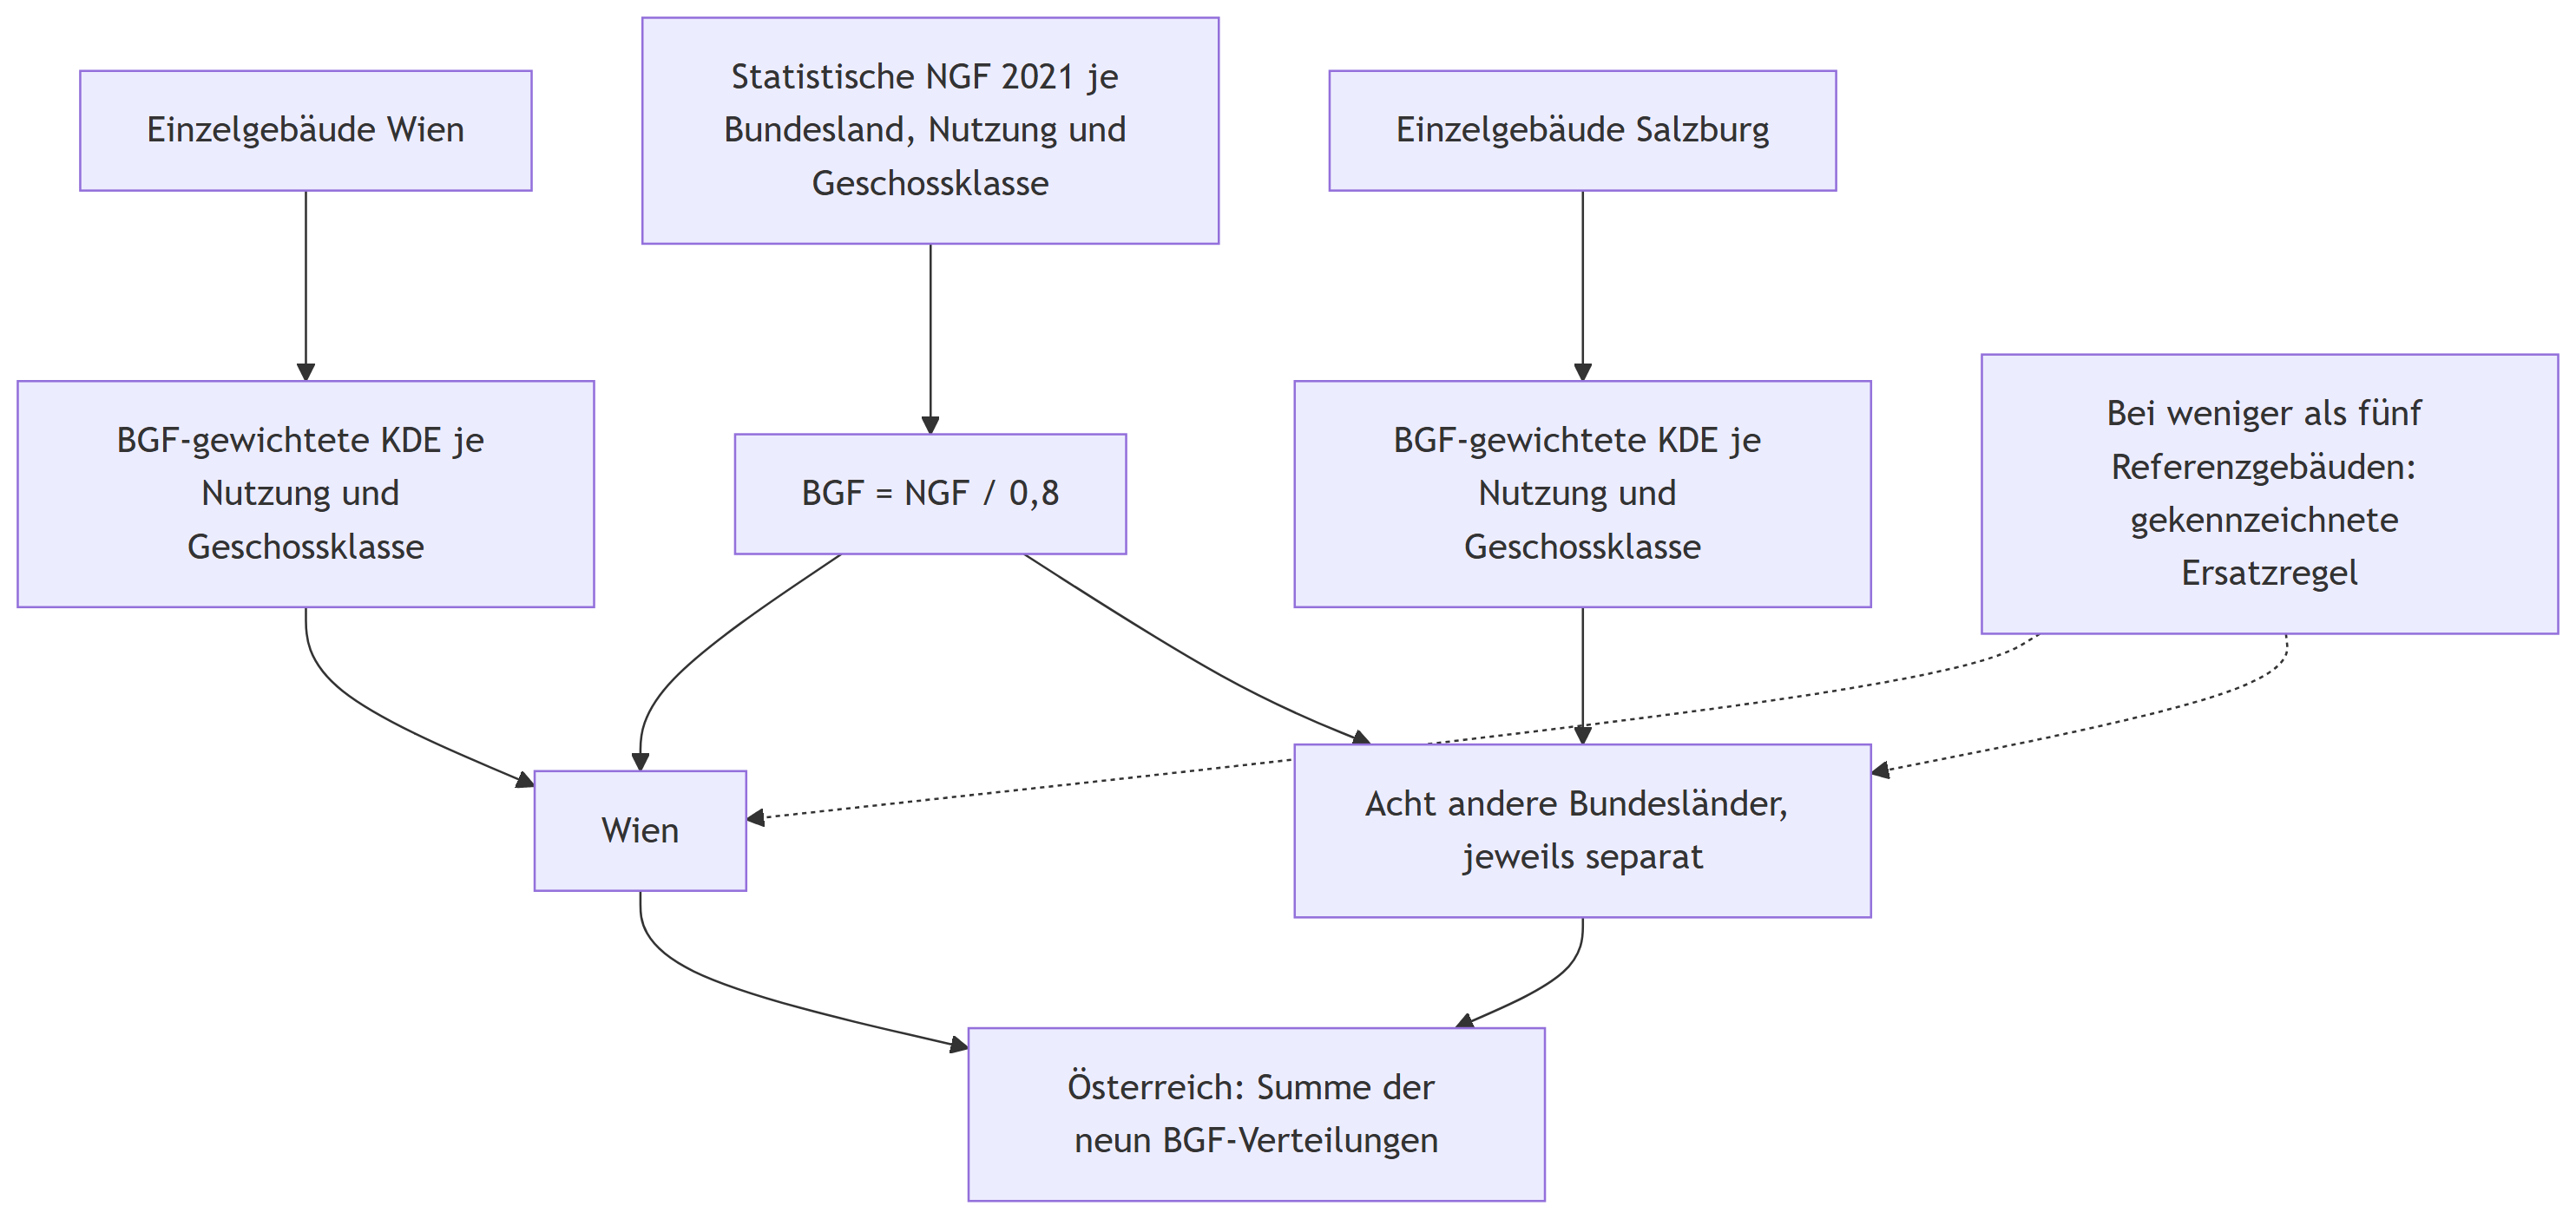
\includegraphics[width=12.1in,height=5.73in]{Berechnungen/gfz_at/GFZ_AT_Analyse_Anhang_files/figure-latex/mermaid-figure-1.png}

}

\caption{\label{fig-gfz-methodik}Bundeslandweise Hochrechnung der
GFZ-Verteilung. Ersatzreferenzen werden je Zielkombination ausdrücklich
ausgewiesen.}

\end{figure}%

\begin{Shaded}
\begin{Highlighting}[]
\CommentTok{\# Modellparameter – hier zentral editierbar}
\ImportTok{from}\NormalTok{ pathlib }\ImportTok{import}\NormalTok{ Path}
\ImportTok{import}\NormalTok{ hashlib}
\ImportTok{import}\NormalTok{ json}
\ImportTok{import}\NormalTok{ textwrap}
\ImportTok{import}\NormalTok{ numpy }\ImportTok{as}\NormalTok{ np}
\ImportTok{import}\NormalTok{ pandas }\ImportTok{as}\NormalTok{ pd}
\ImportTok{import}\NormalTok{ matplotlib.pyplot }\ImportTok{as}\NormalTok{ plt}
\ImportTok{from}\NormalTok{ matplotlib.ticker }\ImportTok{import}\NormalTok{ MultipleLocator}
\ImportTok{from}\NormalTok{ scipy.stats }\ImportTok{import}\NormalTok{ gaussian\_kde}
\ImportTok{from}\NormalTok{ IPython.display }\ImportTok{import}\NormalTok{ display}

\NormalTok{DATA }\OperatorTok{=}\NormalTok{ Path(}\StringTok{"data"}\NormalTok{)                    }\CommentTok{\# ggf. an Quarto{-}Projektstruktur anpassen}
\NormalTok{BUILDINGS }\OperatorTok{=}\NormalTok{ DATA }\OperatorTok{/} \StringTok{"rohdaten\_python.xlsx"}
\NormalTok{STATISTICS }\OperatorTok{=}\NormalTok{ DATA }\OperatorTok{/} \StringTok{"GFZ\_Analyse\_AT.xlsx"}
\NormalTok{OUT }\OperatorTok{=}\NormalTok{ Path(}\StringTok{"outputs/recalculated"}\NormalTok{)}
\NormalTok{OUT.mkdir(parents}\OperatorTok{=}\VariableTok{True}\NormalTok{, exist\_ok}\OperatorTok{=}\VariableTok{True}\NormalTok{)}

\NormalTok{NGF\_PER\_BGF }\OperatorTok{=} \FloatTok{0.8}
\NormalTok{GFZ\_STEP }\OperatorTok{=} \FloatTok{0.1}
\NormalTok{GFZ\_MAX }\OperatorTok{=} \FloatTok{20.0}
\NormalTok{PLOT\_GFZ\_MAX }\OperatorTok{=} \FloatTok{8.0}                 \CommentTok{\# nur Sichtfenster, keine Kürzung der Bilanz}
\NormalTok{MIN\_SAMPLES }\OperatorTok{=} \DecValTok{5}
\NormalTok{FALLBACK }\OperatorTok{=} \StringTok{"vienna"}                \CommentTok{\# "vienna": gekennzeichnete Ersatzregel; "error": Abbruch}
\NormalTok{METHOD }\OperatorTok{=} \StringTok{"kde"}                    \CommentTok{\# "kde" oder zu Diagnosezwecken "histogram"}

\NormalTok{PROVINCES }\OperatorTok{=}\NormalTok{ [}\StringTok{"Burgenland"}\NormalTok{, }\StringTok{"Kärnten"}\NormalTok{, }\StringTok{"Niederösterreich"}\NormalTok{, }\StringTok{"Oberösterreich"}\NormalTok{,}
             \StringTok{"Salzburg"}\NormalTok{, }\StringTok{"Steiermark"}\NormalTok{, }\StringTok{"Tirol"}\NormalTok{, }\StringTok{"Vorarlberg"}\NormalTok{, }\StringTok{"Wien"}\NormalTok{]}
\NormalTok{STOREYS }\OperatorTok{=}\NormalTok{ [}\StringTok{"1"}\NormalTok{, }\StringTok{"2"}\NormalTok{, }\StringTok{"3"}\NormalTok{, }\StringTok{"4"}\NormalTok{, }\StringTok{"5"}\NormalTok{, }\StringTok{"6{-}10"}\NormalTok{, }\StringTok{"11+"}\NormalTok{]}
\NormalTok{USES }\OperatorTok{=}\NormalTok{ [}\StringTok{"Hotels o.Ä."}\NormalTok{, }\StringTok{"Büronutzung"}\NormalTok{, }\StringTok{"Groß{-} und Einzelhandelsgebäude"}\NormalTok{,}
        \StringTok{"Verkehrs{-} und Nachrichtenwesen"}\NormalTok{, }\StringTok{"Industrie und Lagerung"}\NormalTok{,}
        \StringTok{"Kultur, Freizeit, Bildung und Gesundheit"}\NormalTok{, }\StringTok{"Gemeinschaftsgebäude"}\NormalTok{,}
        \StringTok{"Mehrfamilienhaus"}\NormalTok{, }\StringTok{"Ein{-} und Zweifamilienhäuser"}\NormalTok{]}

\CommentTok{\# Einheitliche Farben und Anordnung für ALLE Diagramme}
\NormalTok{COLORS }\OperatorTok{=}\NormalTok{ \{}
    \StringTok{"Groß{-} und Einzelhandelsgebäude"}\NormalTok{: }\StringTok{"\#abd7e7"}\NormalTok{,}
    \StringTok{"Büronutzung"}\NormalTok{: }\StringTok{"\#81c9e6"}\NormalTok{,}
    \StringTok{"Hotels o.Ä."}\NormalTok{: }\StringTok{"\#3e82b8"}\NormalTok{,}
    \StringTok{"Industrie und Lagerung"}\NormalTok{: }\StringTok{"\#405d77"}\NormalTok{,}
    \StringTok{"Ein{-} und Zweifamilienhäuser"}\NormalTok{: }\StringTok{"\#ff9800"}\NormalTok{,}
    \StringTok{"Mehrfamilienhaus"}\NormalTok{: }\StringTok{"\#ff5c48"}\NormalTok{,}
    \StringTok{"Gemeinschaftsgebäude"}\NormalTok{: }\StringTok{"\#dca51b"}\NormalTok{,}
    \StringTok{"Kultur, Freizeit, Bildung und Gesundheit"}\NormalTok{: }\StringTok{"\#92009a"}\NormalTok{,}
    \StringTok{"Verkehrs{-} und Nachrichtenwesen"}\NormalTok{: }\StringTok{"\#a4a4a4"}\NormalTok{,}
\NormalTok{\}}
\NormalTok{PLOT\_USE\_ORDER }\OperatorTok{=} \BuiltInTok{list}\NormalTok{(COLORS)}
\NormalTok{plt.rcParams.update(\{}\StringTok{"font.size"}\NormalTok{: }\DecValTok{10}\NormalTok{, }\StringTok{"axes.spines.top"}\NormalTok{: }\VariableTok{False}\NormalTok{,}
                     \StringTok{"axes.spines.right"}\NormalTok{: }\VariableTok{False}\NormalTok{, }\StringTok{"figure.dpi"}\NormalTok{: }\DecValTok{120}\NormalTok{\})}

\ControlFlowTok{if} \KeywordTok{not}\NormalTok{ (}\DecValTok{0} \OperatorTok{\textless{}}\NormalTok{ NGF\_PER\_BGF }\OperatorTok{\textless{}=} \DecValTok{1} \KeywordTok{and}\NormalTok{ MIN\_SAMPLES }\OperatorTok{\textgreater{}=} \DecValTok{2}\NormalTok{):}
    \ControlFlowTok{raise} \PreprocessorTok{ValueError}\NormalTok{(}\StringTok{"NGF/BGF bzw. Stichprobenminimum unzulässig"}\NormalTok{)}
\ControlFlowTok{if} \KeywordTok{not}\NormalTok{ np.isclose(}\BuiltInTok{round}\NormalTok{(GFZ\_MAX }\OperatorTok{/}\NormalTok{ GFZ\_STEP) }\OperatorTok{*}\NormalTok{ GFZ\_STEP, GFZ\_MAX):}
    \ControlFlowTok{raise} \PreprocessorTok{ValueError}\NormalTok{(}\StringTok{"GFZ\_MAX muss ein Vielfaches von GFZ\_STEP sein"}\NormalTok{)}
\ControlFlowTok{for}\NormalTok{ p }\KeywordTok{in}\NormalTok{ (BUILDINGS, STATISTICS):}
    \ControlFlowTok{if} \KeywordTok{not}\NormalTok{ p.is\_file():}
        \ControlFlowTok{raise} \PreprocessorTok{FileNotFoundError}\NormalTok{(}\SpecialStringTok{f"Quelldatei fehlt: }\SpecialCharTok{\{}\NormalTok{p}\SpecialCharTok{.}\NormalTok{resolve()}\SpecialCharTok{\}}\SpecialStringTok{ – Pfad in der Parameterzelle setzen"}\NormalTok{)}
\end{Highlighting}
\end{Shaded}

\section{2. Eingangsdaten und Plausibilisierung der
Einzelgebäude}\label{eingangsdaten-und-plausibilisierung-der-einzelgebuxe4ude}

Die Originaldaten bleiben bei der Einlesung erhalten. Für die
Verteilungsbildung werden nur Datensätze mit positiver, endlicher BGF
und GFZ bis 20 berücksichtigt. Nicht zu den neun Zielgruppen gehörende
Hauptnutzungen sowie nicht aus Wien oder Salzburg stammende
Referenzgebäude werden ausgeschlossen. Diese Verluste werden explizit
ausgewiesen.

Die beiden Unterkategorien „Mehrfamilienhaus klein`` und
„Mehrfamilienhaus groß`` der gebäudescharfen Daten werden für den
Vergleich mit der statistischen Klassifikation als „Mehrfamilienhaus``
zusammengefasst. Die Zuordnung wird \textbf{nicht} für andere unbekannte
Nutzungsklassen stillschweigend ergänzt.

\begin{Shaded}
\begin{Highlighting}[]
\CommentTok{\# Eingabeformate CSV oder Excel (reiner Dateiimport; keine Modellrechnung)}
\ControlFlowTok{if}\NormalTok{ BUILDINGS.suffix.lower() }\OperatorTok{==} \StringTok{".csv"}\NormalTok{:}
\NormalTok{    samples\_raw }\OperatorTok{=}\NormalTok{ pd.read\_csv(BUILDINGS, dtype}\OperatorTok{=}\NormalTok{\{}\StringTok{"GK"}\NormalTok{: }\BuiltInTok{str}\NormalTok{\}, low\_memory}\OperatorTok{=}\VariableTok{False}\NormalTok{)}
\ControlFlowTok{else}\NormalTok{:}
\NormalTok{    samples\_raw }\OperatorTok{=}\NormalTok{ pd.read\_excel(BUILDINGS, sheet\_name}\OperatorTok{=}\StringTok{"Rohdaten"}\NormalTok{, dtype}\OperatorTok{=}\NormalTok{\{}\StringTok{"GK"}\NormalTok{: }\BuiltInTok{str}\NormalTok{\})}

\NormalTok{required\_samples }\OperatorTok{=}\NormalTok{ [}\StringTok{"Bundesland"}\NormalTok{, }\StringTok{"GK"}\NormalTok{, }\StringTok{"GWR\_Nutzung"}\NormalTok{, }\StringTok{"GFZ"}\NormalTok{, }\StringTok{"BGF"}\NormalTok{]}
\NormalTok{missing }\OperatorTok{=} \BuiltInTok{sorted}\NormalTok{(}\BuiltInTok{set}\NormalTok{(required\_samples) }\OperatorTok{{-}} \BuiltInTok{set}\NormalTok{(samples\_raw))}
\ControlFlowTok{if}\NormalTok{ missing:}
    \ControlFlowTok{raise} \PreprocessorTok{ValueError}\NormalTok{(}\SpecialStringTok{f"Referenzdatei: Spalten fehlen: }\SpecialCharTok{\{}\NormalTok{missing}\SpecialCharTok{\}}\SpecialStringTok{"}\NormalTok{)}

\NormalTok{samples }\OperatorTok{=}\NormalTok{ samples\_raw[required\_samples].copy()}
\CommentTok{\# Normalisierung der in den Originaldateien vorkommenden Geschoss{-}Bezeichnungen}
\NormalTok{samples[}\StringTok{"GK"}\NormalTok{] }\OperatorTok{=}\NormalTok{ (samples[}\StringTok{"GK"}\NormalTok{].astype(}\BuiltInTok{str}\NormalTok{).}\BuiltInTok{str}\NormalTok{.strip().}\BuiltInTok{str}\NormalTok{.lower()}
\NormalTok{                 .}\BuiltInTok{str}\NormalTok{.replace(}\VerbatimStringTok{r"}\CharTok{\textbackslash{}.}\VerbatimStringTok{0}\DecValTok{$}\VerbatimStringTok{"}\NormalTok{, }\StringTok{""}\NormalTok{, regex}\OperatorTok{=}\VariableTok{True}\NormalTok{)}
\NormalTok{                 .replace(\{}\StringTok{"6 bis 10"}\NormalTok{: }\StringTok{"6{-}10"}\NormalTok{, }\StringTok{"6–10"}\NormalTok{: }\StringTok{"6{-}10"}\NormalTok{, }\StringTok{"6010"}\NormalTok{: }\StringTok{"6{-}10"}\NormalTok{,}
                           \StringTok{"6.0 bis 10.0"}\NormalTok{: }\StringTok{"6{-}10"}\NormalTok{, }\StringTok{"11 und mehr"}\NormalTok{: }\StringTok{"11+"}\NormalTok{,}
                           \StringTok{"11 oder mehr"}\NormalTok{: }\StringTok{"11+"}\NormalTok{, }\StringTok{"11plus"}\NormalTok{: }\StringTok{"11+"}\NormalTok{\}))}
\NormalTok{samples[}\StringTok{"GWR\_Nutzung"}\NormalTok{] }\OperatorTok{=}\NormalTok{ samples[}\StringTok{"GWR\_Nutzung"}\NormalTok{].astype(}\BuiltInTok{str}\NormalTok{).}\BuiltInTok{str}\NormalTok{.strip().replace(\{}
    \StringTok{"Mehrfamilienhaus klein"}\NormalTok{: }\StringTok{"Mehrfamilienhaus"}\NormalTok{,}
    \StringTok{"Mehrfamilienhaus groß"}\NormalTok{: }\StringTok{"Mehrfamilienhaus"}\NormalTok{,}
\NormalTok{\})}
\NormalTok{samples[}\StringTok{"GFZ"}\NormalTok{] }\OperatorTok{=}\NormalTok{ pd.to\_numeric(samples[}\StringTok{"GFZ"}\NormalTok{], errors}\OperatorTok{=}\StringTok{"coerce"}\NormalTok{)}
\NormalTok{samples[}\StringTok{"BGF"}\NormalTok{] }\OperatorTok{=}\NormalTok{ pd.to\_numeric(samples[}\StringTok{"BGF"}\NormalTok{], errors}\OperatorTok{=}\StringTok{"coerce"}\NormalTok{)}

\NormalTok{unknown\_gk }\OperatorTok{=} \BuiltInTok{sorted}\NormalTok{(}\BuiltInTok{set}\NormalTok{(samples[}\StringTok{"GK"}\NormalTok{]) }\OperatorTok{{-}} \BuiltInTok{set}\NormalTok{(STOREYS))}
\ControlFlowTok{if}\NormalTok{ unknown\_gk:}
    \ControlFlowTok{raise} \PreprocessorTok{ValueError}\NormalTok{(}\SpecialStringTok{f"Unbekannte Geschossklassen in Gebäudedaten: }\SpecialCharTok{\{}\NormalTok{unknown\_gk}\SpecialCharTok{\}}\SpecialStringTok{"}\NormalTok{)}

\NormalTok{exclude\_usage }\OperatorTok{=} \OperatorTok{\textasciitilde{}}\NormalTok{samples[}\StringTok{"GWR\_Nutzung"}\NormalTok{].isin(USES)}
\NormalTok{exclude\_numeric }\OperatorTok{=}\NormalTok{ (}\OperatorTok{\textasciitilde{}}\NormalTok{np.isfinite(samples[}\StringTok{"GFZ"}\NormalTok{]) }\OperatorTok{|} \OperatorTok{\textasciitilde{}}\NormalTok{np.isfinite(samples[}\StringTok{"BGF"}\NormalTok{])}
                   \OperatorTok{|}\NormalTok{ (samples[}\StringTok{"GFZ"}\NormalTok{] }\OperatorTok{\textless{}=} \DecValTok{0}\NormalTok{) }\OperatorTok{|}\NormalTok{ (samples[}\StringTok{"BGF"}\NormalTok{] }\OperatorTok{\textless{}=} \DecValTok{0}\NormalTok{))}
\NormalTok{exclude\_max }\OperatorTok{=}\NormalTok{ samples[}\StringTok{"GFZ"}\NormalTok{] }\OperatorTok{\textgreater{}}\NormalTok{ GFZ\_MAX}
\NormalTok{exclude\_region }\OperatorTok{=} \OperatorTok{\textasciitilde{}}\NormalTok{samples[}\StringTok{"Bundesland"}\NormalTok{].isin([}\StringTok{"Wien"}\NormalTok{, }\StringTok{"Salzburg"}\NormalTok{])}
\NormalTok{exclude\_any }\OperatorTok{=}\NormalTok{ exclude\_usage }\OperatorTok{|}\NormalTok{ exclude\_numeric }\OperatorTok{|}\NormalTok{ exclude\_max }\OperatorTok{|}\NormalTok{ exclude\_region}

\NormalTok{selection\_report }\OperatorTok{=}\NormalTok{ pd.Series(\{}
    \StringTok{"Originale Gebäudezeilen"}\NormalTok{: }\BuiltInTok{len}\NormalTok{(samples),}
    \StringTok{"Nicht abgedeckte Nutzungen"}\NormalTok{: }\BuiltInTok{int}\NormalTok{(exclude\_usage.}\BuiltInTok{sum}\NormalTok{()),}
    \StringTok{"Ungültige GFZ/BGF"}\NormalTok{: }\BuiltInTok{int}\NormalTok{(exclude\_numeric.}\BuiltInTok{sum}\NormalTok{()),}
    \StringTok{"GFZ über Modellgrenze"}\NormalTok{: }\BuiltInTok{int}\NormalTok{(exclude\_max.}\BuiltInTok{sum}\NormalTok{()),}
    \StringTok{"Andere Referenzregionen"}\NormalTok{: }\BuiltInTok{int}\NormalTok{(exclude\_region.}\BuiltInTok{sum}\NormalTok{()),}
    \StringTok{"Entfallene Zeilen (Vereinigung)"}\NormalTok{: }\BuiltInTok{int}\NormalTok{(exclude\_any.}\BuiltInTok{sum}\NormalTok{()),}
    \StringTok{"Verwendete Referenzgebäude"}\NormalTok{: }\BuiltInTok{int}\NormalTok{((}\OperatorTok{\textasciitilde{}}\NormalTok{exclude\_any).}\BuiltInTok{sum}\NormalTok{()),}
\NormalTok{\}, name}\OperatorTok{=}\StringTok{"Anzahl"}\NormalTok{)}
\NormalTok{display(selection\_report.to\_frame())}
\NormalTok{samples }\OperatorTok{=}\NormalTok{ samples.loc[}\OperatorTok{\textasciitilde{}}\NormalTok{exclude\_any].copy()}
\end{Highlighting}
\end{Shaded}

{\def\LTcaptype{none} % do not increment counter
\begin{longtable}[]{@{}ll@{}}
\toprule\noalign{}
& Anzahl \\
\midrule\noalign{}
\endhead
\bottomrule\noalign{}
\endlastfoot
Originale Gebäudezeilen & 170163 \\
Nicht abgedeckte Nutzungen & 11811 \\
Ungültige GFZ/BGF & 0 \\
GFZ über Modellgrenze & 2 \\
Andere Referenzregionen & 0 \\
Entfallene Zeilen (Vereinigung) & 11813 \\
Verwendete Referenzgebäude & 158350 \\
\end{longtable}
}

\subsection{Deskriptive Auswertung der
Referenzstichproben}\label{deskriptive-auswertung-der-referenzstichproben}

Die nachfolgenden Tabellen berichten \textbf{Gebäudezahlen, erfasste BGF
und GFZ} der zwei Stichproben. Sie sind keine bundesweiten
Gebäudeflächen. Die mittlere GFZ wird mit der BGF der Einzelgebäude
gewichtet; dadurch entspricht sie dem Flächenbezug der späteren KDE. Die
zusätzlich angegebenen Quartile sind ungewichtete Quantile der einzelnen
Gebäude und dienen ausschließlich der Stichprobenbeschreibung.

\begin{Shaded}
\begin{Highlighting}[]
\CommentTok{\# Überblick nach Referenzregion und Nutzung}
\NormalTok{samples\_desc }\OperatorTok{=}\NormalTok{ (samples.groupby([}\StringTok{"Bundesland"}\NormalTok{, }\StringTok{"GWR\_Nutzung"}\NormalTok{], observed}\OperatorTok{=}\VariableTok{True}\NormalTok{)}
\NormalTok{    .agg(Gebaeude}\OperatorTok{=}\NormalTok{(}\StringTok{"GFZ"}\NormalTok{, }\StringTok{"size"}\NormalTok{), BGF\_m2}\OperatorTok{=}\NormalTok{(}\StringTok{"BGF"}\NormalTok{, }\StringTok{"sum"}\NormalTok{),}
\NormalTok{         GFZ\_Median}\OperatorTok{=}\NormalTok{(}\StringTok{"GFZ"}\NormalTok{, }\StringTok{"median"}\NormalTok{), GFZ\_P25}\OperatorTok{=}\NormalTok{(}\StringTok{"GFZ"}\NormalTok{, }\KeywordTok{lambda}\NormalTok{ x: x.quantile(}\FloatTok{.25}\NormalTok{)),}
\NormalTok{         GFZ\_P75}\OperatorTok{=}\NormalTok{(}\StringTok{"GFZ"}\NormalTok{, }\KeywordTok{lambda}\NormalTok{ x: x.quantile(}\FloatTok{.75}\NormalTok{))).reset\_index())}
\NormalTok{weighted\_gfz }\OperatorTok{=}\NormalTok{ (samples.assign(GFZ\_x\_BGF}\OperatorTok{=}\NormalTok{samples.GFZ }\OperatorTok{*}\NormalTok{ samples.BGF)}
\NormalTok{    .groupby([}\StringTok{"Bundesland"}\NormalTok{, }\StringTok{"GWR\_Nutzung"}\NormalTok{])[[}\StringTok{"GFZ\_x\_BGF"}\NormalTok{, }\StringTok{"BGF"}\NormalTok{]].}\BuiltInTok{sum}\NormalTok{())}
\NormalTok{weighted\_gfz }\OperatorTok{=}\NormalTok{ (weighted\_gfz.GFZ\_x\_BGF }\OperatorTok{/}\NormalTok{ weighted\_gfz.BGF).rename(}\StringTok{"GFZ\_flächengewichtet"}\NormalTok{)}
\NormalTok{samples\_desc }\OperatorTok{=}\NormalTok{ samples\_desc.merge(weighted\_gfz.reset\_index(), on}\OperatorTok{=}\NormalTok{[}\StringTok{"Bundesland"}\NormalTok{, }\StringTok{"GWR\_Nutzung"}\NormalTok{])}
\NormalTok{samples\_desc[}\StringTok{"BGF\_Mio\_m2"}\NormalTok{] }\OperatorTok{=}\NormalTok{ samples\_desc[}\StringTok{"BGF\_m2"}\NormalTok{] }\OperatorTok{/} \FloatTok{1e6}
\NormalTok{display(samples\_desc[[}\StringTok{"Bundesland"}\NormalTok{, }\StringTok{"GWR\_Nutzung"}\NormalTok{, }\StringTok{"Gebaeude"}\NormalTok{, }\StringTok{"BGF\_Mio\_m2"}\NormalTok{,}
                      \StringTok{"GFZ\_Median"}\NormalTok{, }\StringTok{"GFZ\_flächengewichtet"}\NormalTok{, }\StringTok{"GFZ\_P25"}\NormalTok{, }\StringTok{"GFZ\_P75"}\NormalTok{]].}\BuiltInTok{round}\NormalTok{(}\DecValTok{3}\NormalTok{))}

\CommentTok{\# Fallzahlen je Referenz{-}/Geschossklasse (wichtig für Ersatzregel)}
\NormalTok{reference\_coverage }\OperatorTok{=}\NormalTok{ samples.groupby([}\StringTok{"Bundesland"}\NormalTok{, }\StringTok{"GK"}\NormalTok{, }\StringTok{"GWR\_Nutzung"}\NormalTok{]).size().rename(}\StringTok{"n"}\NormalTok{).reset\_index()}
\NormalTok{display(reference\_coverage.pivot\_table(index}\OperatorTok{=}\NormalTok{[}\StringTok{"Bundesland"}\NormalTok{, }\StringTok{"GK"}\NormalTok{], columns}\OperatorTok{=}\StringTok{"GWR\_Nutzung"}\NormalTok{,}
\NormalTok{                                       values}\OperatorTok{=}\StringTok{"n"}\NormalTok{, aggfunc}\OperatorTok{=}\StringTok{"sum"}\NormalTok{, fill\_value}\OperatorTok{=}\DecValTok{0}\NormalTok{).astype(}\BuiltInTok{int}\NormalTok{))}
\end{Highlighting}
\end{Shaded}

{\def\LTcaptype{none} % do not increment counter
\begin{longtable}[]{@{}lllllllll@{}}
\toprule\noalign{}
& Bundesland & GWR\_Nutzung & Gebaeude & BGF\_Mio\_m2 & GFZ\_Median &
GFZ\_flächengewichtet & GFZ\_P25 & GFZ\_P75 \\
\midrule\noalign{}
\endhead
\bottomrule\noalign{}
\endlastfoot
0 & Salzburg & Büronutzung & 1268 & 1.770 & 0.959 & 1.817 & 0.598 &
1.705 \\
1 & Salzburg & Ein- und Zweifamilienhäuser & 38063 & 11.231 & 0.460 &
0.724 & 0.335 & 0.640 \\
2 & Salzburg & Groß- und Einzelhandelsgebäude & 1670 & 1.900 & 0.872 &
1.476 & 0.505 & 1.619 \\
3 & Salzburg & Hotels o.Ä. & 2971 & 3.063 & 0.808 & 1.729 & 0.489 &
1.541 \\
4 & Salzburg & Industrie und Lagerung & 2397 & 3.337 & 0.554 & 1.162 &
0.341 & 0.879 \\
5 & Salzburg & Kultur, Freizeit, Bildung und Gesundheit & 681 & 1.231 &
0.752 & 1.871 & 0.394 & 1.388 \\
6 & Salzburg & Mehrfamilienhaus & 23238 & 16.104 & 0.673 & 1.362 & 0.470
& 1.112 \\
7 & Salzburg & Verkehrs- und Nachrichtenwesen & 78 & 0.084 & 0.398 &
1.604 & 0.241 & 0.953 \\
8 & Wien & Büronutzung & 4398 & 15.717 & 3.320 & 4.636 & 1.713 &
4.816 \\
9 & Wien & Ein- und Zweifamilienhäuser & 52141 & 15.382 & 0.454 & 1.880
& 0.258 & 1.292 \\
10 & Wien & Gemeinschaftsgebäude & 104 & 0.425 & 2.214 & 3.672 & 0.793 &
4.012 \\
11 & Wien & Groß- und Einzelhandelsgebäude & 631 & 1.877 & 0.891 & 2.599
& 0.398 & 1.824 \\
12 & Wien & Hotels o.Ä. & 707 & 2.667 & 2.531 & 6.534 & 0.992 & 4.534 \\
13 & Wien & Industrie und Lagerung & 1437 & 3.176 & 1.066 & 2.402 &
0.600 & 1.916 \\
14 & Wien & Kultur, Freizeit, Bildung und Gesundheit & 661 & 4.363 &
2.884 & 3.531 & 0.969 & 4.135 \\
15 & Wien & Mehrfamilienhaus & 27589 & 64.627 & 3.782 & 4.233 & 2.647 &
4.707 \\
16 & Wien & Verkehrs- und Nachrichtenwesen & 316 & 0.580 & 0.772 & 2.304
& 0.384 & 1.541 \\
\end{longtable}
}

{\def\LTcaptype{none} % do not increment counter
\begin{longtable}[]{@{}lllllllllll@{}}
\toprule\noalign{}
& GWR\_Nutzung & Büronutzung & Ein- und Zweifamilienhäuser &
Gemeinschaftsgebäude & Groß- und Einzelhandelsgebäude & Hotels o.Ä. &
Industrie und Lagerung & Kultur, Freizeit, Bildung und Gesundheit &
Mehrfamilienhaus & Verkehrs- und Nachrichtenwesen \\
Bundesland & GK & & & & & & & & & \\
\midrule\noalign{}
\endhead
\bottomrule\noalign{}
\endlastfoot
\multirow{7}{*}{Salzburg} & 1 & 63 & 576 & 0 & 240 & 113 & 665 & 85 &
127 & 29 \\
& 11+ & 0 & 0 & 0 & 0 & 0 & 0 & 0 & 1 & 0 \\
& 2 & 334 & 19517 & 0 & 601 & 906 & 1118 & 206 & 5019 & 23 \\
& 3 & 431 & 15912 & 0 & 551 & 1173 & 401 & 198 & 11496 & 13 \\
& 4 & 218 & 1471 & 0 & 166 & 539 & 129 & 110 & 3877 & 9 \\
& 5 & 115 & 303 & 0 & 65 & 175 & 50 & 49 & 1521 & 1 \\
& 6-10 & 107 & 284 & 0 & 47 & 65 & 34 & 33 & 1197 & 3 \\
\multirow{7}{*}{Wien} & 1 & 137 & 15342 & 5 & 164 & 56 & 310 & 45 & 100
& 59 \\
& 11+ & 103 & 32 & 2 & 4 & 20 & 5 & 40 & 234 & 1 \\
& 2 & 398 & 16886 & 11 & 153 & 124 & 356 & 56 & 820 & 75 \\
& 3 & 457 & 14311 & 13 & 102 & 94 & 215 & 50 & 1632 & 79 \\
& 4 & 434 & 3622 & 12 & 71 & 46 & 190 & 69 & 2191 & 42 \\
& 5 & 572 & 956 & 16 & 57 & 70 & 194 & 61 & 3322 & 19 \\
& 6-10 & 2297 & 992 & 45 & 80 & 297 & 167 & 340 & 19290 & 41 \\
\end{longtable}
}

\begin{Shaded}
\begin{Highlighting}[]
\NormalTok{fig, ax }\OperatorTok{=}\NormalTok{ plt.subplots(figsize}\OperatorTok{=}\NormalTok{(}\DecValTok{12}\NormalTok{, }\FloatTok{4.5}\NormalTok{), layout}\OperatorTok{=}\StringTok{"constrained"}\NormalTok{)}
\NormalTok{raw\_edges }\OperatorTok{=}\NormalTok{ np.arange(}\DecValTok{0}\NormalTok{, }\DecValTok{5} \OperatorTok{+}\NormalTok{ GFZ\_STEP }\OperatorTok{/} \DecValTok{2}\NormalTok{, GFZ\_STEP)}
\ControlFlowTok{for}\NormalTok{ region, color }\KeywordTok{in}\NormalTok{ [(}\StringTok{"Wien"}\NormalTok{, }\StringTok{"\#955196"}\NormalTok{), (}\StringTok{"Salzburg"}\NormalTok{, }\StringTok{"\#007c83"}\NormalTok{)]:}
\NormalTok{    g }\OperatorTok{=}\NormalTok{ samples.loc[samples.Bundesland }\OperatorTok{==}\NormalTok{ region]}
\NormalTok{    counts, \_ }\OperatorTok{=}\NormalTok{ np.histogram(g.GFZ, bins}\OperatorTok{=}\NormalTok{raw\_edges, weights}\OperatorTok{=}\NormalTok{g.BGF)}
    \CommentTok{\# normiert auf die GESAMTE Referenz{-}BGF (einschließlich GFZ \textgreater{} 5)}
\NormalTok{    ax.step(raw\_edges[:}\OperatorTok{{-}}\DecValTok{1}\NormalTok{], }\DecValTok{100} \OperatorTok{*}\NormalTok{ counts }\OperatorTok{/}\NormalTok{ g.BGF.}\BuiltInTok{sum}\NormalTok{(), where}\OperatorTok{=}\StringTok{"post"}\NormalTok{,}
\NormalTok{            linewidth}\OperatorTok{=}\FloatTok{1.6}\NormalTok{, label}\OperatorTok{=}\NormalTok{region, color}\OperatorTok{=}\NormalTok{color)}
\NormalTok{ax.}\BuiltInTok{set}\NormalTok{(xlim}\OperatorTok{=}\NormalTok{(}\DecValTok{0}\NormalTok{, }\DecValTok{5}\NormalTok{), ylim}\OperatorTok{=}\NormalTok{(}\DecValTok{0}\NormalTok{, }\VariableTok{None}\NormalTok{), xlabel}\OperatorTok{=}\StringTok{"Geschossflächenzahl (GFZ)"}\NormalTok{,}
\NormalTok{       ylabel}\OperatorTok{=}\StringTok{"Anteil Referenz{-}BGF [\% je 0,1 GFZ]"}\NormalTok{)}
\NormalTok{ax.xaxis.set\_major\_locator(MultipleLocator(}\DecValTok{1}\NormalTok{))}
\NormalTok{ax.xaxis.set\_minor\_locator(MultipleLocator(GFZ\_STEP))}
\NormalTok{ax.grid(axis}\OperatorTok{=}\StringTok{"x"}\NormalTok{, alpha}\OperatorTok{=}\FloatTok{.15}\NormalTok{)}
\NormalTok{ax.legend()}
\NormalTok{fig.savefig(OUT }\OperatorTok{/} \StringTok{"gfz\_referenz\_rohstichproben.png"}\NormalTok{, dpi}\OperatorTok{=}\DecValTok{180}\NormalTok{, bbox\_inches}\OperatorTok{=}\StringTok{"tight"}\NormalTok{)}
\NormalTok{plt.show()}
\end{Highlighting}
\end{Shaded}

\begin{figure}[H]

\centering{

\pandocbounded{\includegraphics[keepaspectratio]{Berechnungen/gfz_at/GFZ_AT_Analyse_Anhang_files/figure-pdf/fig-gfz-rohstichproben-output-1.png}}

}

\caption{\label{fig-gfz-rohstichproben}BGF-gewichtete GFZ-Häufigkeit der
bereinigten Referenzgebäude aus Wien und Salzburg. Das Histogramm
beschreibt die Stichprobe, nicht die hochgerechnete österreichische
BGF.}

\end{figure}%

\section{3. Statistische Bestandsdaten 2021: Herkunft, Flächen und
Struktur}\label{statistische-bestandsdaten-2021-herkunft-fluxe4chen-und-struktur}

Für die nationale Hochrechnung bildet die Statistik die verbindliche
\textbf{Mengenbasis}. Aus dem Tabellenblatt \texttt{python} werden die
neun Bundesländer und sieben Geschossklassen mit den neun
Nutzungsgruppen entnommen. Zusätzliche historische Aggregatzeilen („AT
ohne Wien und Salzburg``, „Alles``) werden herausgenommen, damit keine
Doppelzählung entsteht. Die nationale Zeile \texttt{AT} wird nur zur
Kontrolle verwendet.

\textbf{Wichtig für die Diagramme:} Die statistischen Eingangsdaten sind
als \textbf{NGF} abgelegt. Erst die Umrechnung mit
\texttt{NGF\_PER\_BGF\ =\ 0.8} erzeugt die im Anschluss als \textbf{BGF}
dargestellten Flächen. In den Diagrammen wird somit die
\emph{statistisch verankerte, modellierte BGF} gezeigt, nicht eine
ursprünglich als BGF veröffentlichte Größe.

\begin{Shaded}
\begin{Highlighting}[]
\ControlFlowTok{if}\NormalTok{ STATISTICS.suffix.lower() }\OperatorTok{==} \StringTok{".csv"}\NormalTok{:}
\NormalTok{    stats\_raw }\OperatorTok{=}\NormalTok{ pd.read\_csv(STATISTICS, dtype}\OperatorTok{=}\NormalTok{\{}\StringTok{"GK"}\NormalTok{: }\BuiltInTok{str}\NormalTok{\}, low\_memory}\OperatorTok{=}\VariableTok{False}\NormalTok{)}
\ControlFlowTok{else}\NormalTok{:}
\NormalTok{    stats\_raw }\OperatorTok{=}\NormalTok{ pd.read\_excel(STATISTICS, sheet\_name}\OperatorTok{=}\StringTok{"python"}\NormalTok{, dtype}\OperatorTok{=}\NormalTok{\{}\StringTok{"GK"}\NormalTok{: }\BuiltInTok{str}\NormalTok{\})}

\NormalTok{missing }\OperatorTok{=} \BuiltInTok{sorted}\NormalTok{(}\BuiltInTok{set}\NormalTok{([}\StringTok{"NUTS"}\NormalTok{, }\StringTok{"GK"}\NormalTok{, }\OperatorTok{*}\NormalTok{USES]) }\OperatorTok{{-}} \BuiltInTok{set}\NormalTok{(stats\_raw.columns))}
\ControlFlowTok{if}\NormalTok{ missing:}
    \ControlFlowTok{raise} \PreprocessorTok{ValueError}\NormalTok{(}\SpecialStringTok{f"Statistikdatei: Spalten fehlen: }\SpecialCharTok{\{}\NormalTok{missing}\SpecialCharTok{\}}\SpecialStringTok{"}\NormalTok{)}

\NormalTok{legacy\_aggregates }\OperatorTok{=}\NormalTok{ [}\StringTok{"AT ohne Wien und Salzburg"}\NormalTok{, }\StringTok{"Alles"}\NormalTok{]}
\NormalTok{removed\_aggregates }\OperatorTok{=}\NormalTok{ stats\_raw.loc[stats\_raw.NUTS.isin(legacy\_aggregates), }\StringTok{"NUTS"}\NormalTok{].value\_counts()}
\NormalTok{stats }\OperatorTok{=}\NormalTok{ stats\_raw.loc[}\OperatorTok{\textasciitilde{}}\NormalTok{stats\_raw.NUTS.isin(legacy\_aggregates), [}\StringTok{"NUTS"}\NormalTok{, }\StringTok{"GK"}\NormalTok{, }\OperatorTok{*}\NormalTok{USES]].copy()}
\NormalTok{stats[}\StringTok{"GK"}\NormalTok{] }\OperatorTok{=}\NormalTok{ (stats[}\StringTok{"GK"}\NormalTok{].astype(}\BuiltInTok{str}\NormalTok{).}\BuiltInTok{str}\NormalTok{.strip().}\BuiltInTok{str}\NormalTok{.lower()}
\NormalTok{                .}\BuiltInTok{str}\NormalTok{.replace(}\VerbatimStringTok{r"}\CharTok{\textbackslash{}.}\VerbatimStringTok{0}\DecValTok{$}\VerbatimStringTok{"}\NormalTok{, }\StringTok{""}\NormalTok{, regex}\OperatorTok{=}\VariableTok{True}\NormalTok{)}
\NormalTok{                .replace(\{}\StringTok{"6 bis 10"}\NormalTok{: }\StringTok{"6{-}10"}\NormalTok{, }\StringTok{"6–10"}\NormalTok{: }\StringTok{"6{-}10"}\NormalTok{, }\StringTok{"6010"}\NormalTok{: }\StringTok{"6{-}10"}\NormalTok{,}
                          \StringTok{"6.0 bis 10.0"}\NormalTok{: }\StringTok{"6{-}10"}\NormalTok{, }\StringTok{"11 und mehr"}\NormalTok{: }\StringTok{"11+"}\NormalTok{,}
                          \StringTok{"11 oder mehr"}\NormalTok{: }\StringTok{"11+"}\NormalTok{, }\StringTok{"11plus"}\NormalTok{: }\StringTok{"11+"}\NormalTok{\}))}

\NormalTok{bad\_regions }\OperatorTok{=} \BuiltInTok{set}\NormalTok{(stats.NUTS.dropna().astype(}\BuiltInTok{str}\NormalTok{)) }\OperatorTok{{-}} \BuiltInTok{set}\NormalTok{(PROVINCES }\OperatorTok{+}\NormalTok{ [}\StringTok{"AT"}\NormalTok{])}
\ControlFlowTok{if}\NormalTok{ bad\_regions:}
    \ControlFlowTok{raise} \PreprocessorTok{ValueError}\NormalTok{(}\SpecialStringTok{f"Unbekannte Regionen in Statistik: }\SpecialCharTok{\{}\NormalTok{bad\_regions}\SpecialCharTok{\}}\SpecialStringTok{"}\NormalTok{)}
\ControlFlowTok{if}\NormalTok{ stats.duplicated([}\StringTok{"NUTS"}\NormalTok{, }\StringTok{"GK"}\NormalTok{]).}\BuiltInTok{any}\NormalTok{():}
    \ControlFlowTok{raise} \PreprocessorTok{ValueError}\NormalTok{(}\StringTok{"Doppelte Statistikzeilen mit identischem NUTS/GK"}\NormalTok{)}
\NormalTok{missing\_pairs }\OperatorTok{=}\NormalTok{ \{(b, g) }\ControlFlowTok{for}\NormalTok{ b }\KeywordTok{in}\NormalTok{ PROVINCES }\OperatorTok{+}\NormalTok{ [}\StringTok{"AT"}\NormalTok{] }\ControlFlowTok{for}\NormalTok{ g }\KeywordTok{in}\NormalTok{ STOREYS\} }\OperatorTok{{-}} \BuiltInTok{set}\NormalTok{(}\BuiltInTok{zip}\NormalTok{(stats.NUTS, stats.GK))}
\ControlFlowTok{if}\NormalTok{ missing\_pairs:}
    \ControlFlowTok{raise} \PreprocessorTok{ValueError}\NormalTok{(}\SpecialStringTok{f"Geschossklassen in Statistik nicht vollständig: }\SpecialCharTok{\{}\BuiltInTok{sorted}\NormalTok{(missing\_pairs)}\SpecialCharTok{\}}\SpecialStringTok{"}\NormalTok{)}

\ControlFlowTok{for}\NormalTok{ u }\KeywordTok{in}\NormalTok{ USES:}
\NormalTok{    stats[u] }\OperatorTok{=}\NormalTok{ pd.to\_numeric(stats[u], errors}\OperatorTok{=}\StringTok{"raise"}\NormalTok{).fillna(}\DecValTok{0}\NormalTok{)}
\ControlFlowTok{if}\NormalTok{ stats[USES].lt(}\DecValTok{0}\NormalTok{).}\BuiltInTok{any}\NormalTok{().}\BuiltInTok{any}\NormalTok{():}
    \ControlFlowTok{raise} \PreprocessorTok{ValueError}\NormalTok{(}\StringTok{"Statistische NGF enthält negative Werte"}\NormalTok{)}

\CommentTok{\# Statistik: breites Eingangsschema in Bundesland × GK × Nutzung überführen}
\NormalTok{stats\_long }\OperatorTok{=}\NormalTok{ stats.melt(id\_vars}\OperatorTok{=}\NormalTok{[}\StringTok{"NUTS"}\NormalTok{, }\StringTok{"GK"}\NormalTok{], value\_vars}\OperatorTok{=}\NormalTok{USES,}
\NormalTok{                        var\_name}\OperatorTok{=}\StringTok{"GWR\_Nutzung"}\NormalTok{, value\_name}\OperatorTok{=}\StringTok{"NGF\_m2"}\NormalTok{)}
\NormalTok{control\_at }\OperatorTok{=}\NormalTok{ (stats\_long.loc[stats\_long.NUTS }\OperatorTok{==} \StringTok{"AT"}\NormalTok{]}
\NormalTok{              .set\_index([}\StringTok{"GK"}\NormalTok{, }\StringTok{"GWR\_Nutzung"}\NormalTok{])[}\StringTok{"NGF\_m2"}\NormalTok{])}
\NormalTok{provinces\_ngf }\OperatorTok{=}\NormalTok{ stats\_long.loc[stats\_long.NUTS.isin(PROVINCES)].copy()}
\NormalTok{control\_regions }\OperatorTok{=}\NormalTok{ provinces\_ngf.groupby([}\StringTok{"GK"}\NormalTok{, }\StringTok{"GWR\_Nutzung"}\NormalTok{])[}\StringTok{"NGF\_m2"}\NormalTok{].}\BuiltInTok{sum}\NormalTok{()}
\NormalTok{control\_delta }\OperatorTok{=}\NormalTok{ control\_regions.sub(control\_at, fill\_value}\OperatorTok{=}\DecValTok{0}\NormalTok{)}
\ControlFlowTok{if} \KeywordTok{not}\NormalTok{ np.allclose(control\_delta.to\_numpy(), }\DecValTok{0}\NormalTok{, rtol}\OperatorTok{=}\DecValTok{0}\NormalTok{, atol}\OperatorTok{=}\FloatTok{0.01}\NormalTok{):}
    \ControlFlowTok{raise} \PreprocessorTok{AssertionError}\NormalTok{(}\SpecialStringTok{f"Bundesländer ≠ AT{-}Zeile; Beispiele: }\SpecialCharTok{\{}\NormalTok{control\_delta[control\_delta.}\BuiltInTok{abs}\NormalTok{() }\OperatorTok{\textgreater{}} \FloatTok{.01}\NormalTok{]}\SpecialCharTok{.}\NormalTok{head()}\SpecialCharTok{.}\NormalTok{to\_dict()}\SpecialCharTok{\}}\SpecialStringTok{"}\NormalTok{)}

\CommentTok{\# Der explizite Umrechnungsschritt: aus statistischer NGF wird Modell{-}BGF.}
\NormalTok{targets }\OperatorTok{=}\NormalTok{ provinces\_ngf.rename(columns}\OperatorTok{=}\NormalTok{\{}\StringTok{"NUTS"}\NormalTok{: }\StringTok{"Bundesland"}\NormalTok{\}).copy()}
\NormalTok{targets[}\StringTok{"BGF\_target\_m2"}\NormalTok{] }\OperatorTok{=}\NormalTok{ targets[}\StringTok{"NGF\_m2"}\NormalTok{] }\OperatorTok{/}\NormalTok{ NGF\_PER\_BGF}
\BuiltInTok{print}\NormalTok{(}\StringTok{"Historische Summenzeilen ausgeschlossen:"}\NormalTok{, removed\_aggregates.to\_dict())}
\BuiltInTok{print}\NormalTok{(}\SpecialStringTok{f"AT{-}NGF nach Kontrollzeile: }\SpecialCharTok{\{}\NormalTok{control\_at}\SpecialCharTok{.}\BuiltInTok{sum}\NormalTok{()}\OperatorTok{/}\FloatTok{1e6}\SpecialCharTok{:,.3f\}}\SpecialStringTok{ Mio. m²"}\NormalTok{)}
\BuiltInTok{print}\NormalTok{(}\SpecialStringTok{f"AT{-}BGF aus NGF/0,8: }\SpecialCharTok{\{}\NormalTok{targets}\SpecialCharTok{.}\NormalTok{BGF\_target\_m2}\SpecialCharTok{.}\BuiltInTok{sum}\NormalTok{()}\OperatorTok{/}\FloatTok{1e6}\SpecialCharTok{:,.3f\}}\SpecialStringTok{ Mio. m²"}\NormalTok{)}
\BuiltInTok{print}\NormalTok{(}\SpecialStringTok{f"Maximale Differenz zur AT{-}Kontrollzeile: }\SpecialCharTok{\{}\NormalTok{control\_delta}\SpecialCharTok{.}\BuiltInTok{abs}\NormalTok{()}\SpecialCharTok{.}\BuiltInTok{max}\NormalTok{()}\SpecialCharTok{:.6f\}}\SpecialStringTok{ m² NGF"}\NormalTok{)}
\end{Highlighting}
\end{Shaded}

\begin{verbatim}
Historische Summenzeilen ausgeschlossen: {'AT ohne Wien und Salzburg': 7, 'Alles': 1}
AT-NGF nach Kontrollzeile: 847.148 Mio. m²
AT-BGF aus NGF/0,8: 1,058.935 Mio. m²
Maximale Differenz zur AT-Kontrollzeile: 0.000000 m² NGF
\end{verbatim}

\subsection{Deskriptive Statistik des nationalen
Bestandsmodells}\label{deskriptive-statistik-des-nationalen-bestandsmodells}

Die erste Tabelle weist je Bundesland die NGF aus der Statistik, die
daraus abgeleitete BGF und den Anteil an der nationalen Modell-BGF aus.
Anschließend werden die Flächen nach Geschossklasse und Nutzung
ausgewertet. Alle folgenden Flächenbalken verwenden die \textbf{gleichen
neun Nutzungsfarben}, die später auch für die österreichische
GFZ-Verteilung gelten. Ein gestapelter Balken zeigt die absoluten,
summierbaren BGF-Beiträge, keine Gebäudeanzahlen.

\begin{Shaded}
\begin{Highlighting}[]
\NormalTok{stats\_province }\OperatorTok{=}\NormalTok{ (targets.groupby(}\StringTok{"Bundesland"}\NormalTok{, as\_index}\OperatorTok{=}\VariableTok{False}\NormalTok{)[[}\StringTok{"NGF\_m2"}\NormalTok{, }\StringTok{"BGF\_target\_m2"}\NormalTok{]]}
\NormalTok{                  .}\BuiltInTok{sum}\NormalTok{().set\_index(}\StringTok{"Bundesland"}\NormalTok{).reindex(PROVINCES))}
\NormalTok{stats\_province[}\StringTok{"Anteil\_AT\_\%"}\NormalTok{] }\OperatorTok{=} \DecValTok{100} \OperatorTok{*}\NormalTok{ stats\_province.BGF\_target\_m2 }\OperatorTok{/}\NormalTok{ stats\_province.BGF\_target\_m2.}\BuiltInTok{sum}\NormalTok{()}
\NormalTok{stats\_display }\OperatorTok{=}\NormalTok{ stats\_province.copy()}
\NormalTok{stats\_display[}\StringTok{"NGF\_Mio\_m2"}\NormalTok{] }\OperatorTok{=}\NormalTok{ stats\_display.NGF\_m2 }\OperatorTok{/} \FloatTok{1e6}
\NormalTok{stats\_display[}\StringTok{"BGF\_Mio\_m2"}\NormalTok{] }\OperatorTok{=}\NormalTok{ stats\_display.BGF\_target\_m2 }\OperatorTok{/} \FloatTok{1e6}
\NormalTok{display(stats\_display[[}\StringTok{"NGF\_Mio\_m2"}\NormalTok{, }\StringTok{"BGF\_Mio\_m2"}\NormalTok{, }\StringTok{"Anteil\_AT\_\%"}\NormalTok{]].}\BuiltInTok{round}\NormalTok{(}\DecValTok{3}\NormalTok{))}

\NormalTok{stats\_gk }\OperatorTok{=}\NormalTok{ (targets.groupby(}\StringTok{"GK"}\NormalTok{)[}\StringTok{"BGF\_target\_m2"}\NormalTok{].}\BuiltInTok{sum}\NormalTok{()}
\NormalTok{            .reindex(STOREYS).div(}\FloatTok{1e6}\NormalTok{).rename(}\StringTok{"BGF\_Mio\_m2"}\NormalTok{))}
\NormalTok{stats\_use }\OperatorTok{=}\NormalTok{ (targets.groupby(}\StringTok{"GWR\_Nutzung"}\NormalTok{)[}\StringTok{"BGF\_target\_m2"}\NormalTok{].}\BuiltInTok{sum}\NormalTok{()}
\NormalTok{             .reindex(PLOT\_USE\_ORDER).div(}\FloatTok{1e6}\NormalTok{).rename(}\StringTok{"BGF\_Mio\_m2"}\NormalTok{))}
\NormalTok{display(pd.DataFrame(\{}\StringTok{"BGF Mio. m² nach Geschossklasse"}\NormalTok{: stats\_gk\}))}
\NormalTok{display(pd.DataFrame(\{}\StringTok{"BGF Mio. m² nach Hauptnutzung"}\NormalTok{: stats\_use\}).sort\_values(}\StringTok{"BGF Mio. m² nach Hauptnutzung"}\NormalTok{, ascending}\OperatorTok{=}\VariableTok{False}\NormalTok{))}
\end{Highlighting}
\end{Shaded}

{\def\LTcaptype{none} % do not increment counter
\begin{longtable}[]{@{}llll@{}}
\toprule\noalign{}
& NGF\_Mio\_m2 & BGF\_Mio\_m2 & Anteil\_AT\_\% \\
Bundesland & & & \\
\midrule\noalign{}
\endhead
\bottomrule\noalign{}
\endlastfoot
Burgenland & 30.434 & 38.043 & 3.593 \\
Kärnten & 54.446 & 68.058 & 6.427 \\
Niederösterreich & 171.910 & 214.888 & 20.293 \\
Oberösterreich & 157.719 & 197.149 & 18.618 \\
Salzburg & 55.595 & 69.494 & 6.563 \\
Steiermark & 120.031 & 150.038 & 14.169 \\
Tirol & 79.835 & 99.794 & 9.424 \\
Vorarlberg & 37.347 & 46.683 & 4.409 \\
Wien & 139.830 & 174.787 & 16.506 \\
\end{longtable}
}

{\def\LTcaptype{none} % do not increment counter
\begin{longtable}[]{@{}ll@{}}
\toprule\noalign{}
& BGF Mio. m² nach Geschossklasse \\
GK & \\
\midrule\noalign{}
\endhead
\bottomrule\noalign{}
\endlastfoot
1 & 216.827551 \\
2 & 382.613315 \\
3 & 179.588949 \\
4 & 104.302704 \\
5 & 60.409821 \\
6-10 & 103.898680 \\
11+ & 11.293873 \\
\end{longtable}
}

{\def\LTcaptype{none} % do not increment counter
\begin{longtable}[]{@{}ll@{}}
\toprule\noalign{}
& BGF Mio. m² nach Hauptnutzung \\
GWR\_Nutzung & \\
\midrule\noalign{}
\endhead
\bottomrule\noalign{}
\endlastfoot
Ein- und Zweifamilienhäuser & 375.776284 \\
Mehrfamilienhaus & 271.624840 \\
Industrie und Lagerung & 122.853401 \\
Büronutzung & 76.624895 \\
Kultur, Freizeit, Bildung und Gesundheit & 65.894111 \\
Groß- und Einzelhandelsgebäude & 64.865034 \\
Hotels o.Ä. & 51.366923 \\
Gemeinschaftsgebäude & 17.056024 \\
Verkehrs- und Nachrichtenwesen & 12.873381 \\
\end{longtable}
}

\begin{Shaded}
\begin{Highlighting}[]
\CommentTok{\# Statistische BGF nach Bundesland × Hauptnutzung (keine KDE beteiligt)}
\NormalTok{by\_province\_use }\OperatorTok{=}\NormalTok{ (targets.pivot\_table(index}\OperatorTok{=}\StringTok{"Bundesland"}\NormalTok{, columns}\OperatorTok{=}\StringTok{"GWR\_Nutzung"}\NormalTok{,}
\NormalTok{                values}\OperatorTok{=}\StringTok{"BGF\_target\_m2"}\NormalTok{, aggfunc}\OperatorTok{=}\StringTok{"sum"}\NormalTok{, fill\_value}\OperatorTok{=}\DecValTok{0}\NormalTok{)}
\NormalTok{            .reindex(index}\OperatorTok{=}\NormalTok{PROVINCES, columns}\OperatorTok{=}\NormalTok{PLOT\_USE\_ORDER, fill\_value}\OperatorTok{=}\DecValTok{0}\NormalTok{) }\OperatorTok{/} \FloatTok{1e6}\NormalTok{)}
\NormalTok{fig, ax }\OperatorTok{=}\NormalTok{ plt.subplots(figsize}\OperatorTok{=}\NormalTok{(}\DecValTok{13}\NormalTok{, }\FloatTok{6.5}\NormalTok{), layout}\OperatorTok{=}\StringTok{"constrained"}\NormalTok{)}
\NormalTok{left }\OperatorTok{=}\NormalTok{ np.zeros(}\BuiltInTok{len}\NormalTok{(PROVINCES))}
\ControlFlowTok{for}\NormalTok{ usage }\KeywordTok{in}\NormalTok{ PLOT\_USE\_ORDER:}
\NormalTok{    vals }\OperatorTok{=}\NormalTok{ by\_province\_use[usage].to\_numpy()}
\NormalTok{    ax.barh(PROVINCES, vals, left}\OperatorTok{=}\NormalTok{left, label}\OperatorTok{=}\NormalTok{usage, color}\OperatorTok{=}\NormalTok{COLORS[usage],}
\NormalTok{            height}\OperatorTok{=}\FloatTok{.75}\NormalTok{, edgecolor}\OperatorTok{=}\StringTok{"white"}\NormalTok{, linewidth}\OperatorTok{=}\FloatTok{.25}\NormalTok{)}
\NormalTok{    left }\OperatorTok{+=}\NormalTok{ vals}
\CommentTok{\# Gesamtsummen neben den Balken}
\ControlFlowTok{for}\NormalTok{ y, total }\KeywordTok{in} \BuiltInTok{enumerate}\NormalTok{(left):}
\NormalTok{    ax.text(total }\OperatorTok{+} \DecValTok{2}\NormalTok{, y, }\SpecialStringTok{f"}\SpecialCharTok{\{}\NormalTok{total}\SpecialCharTok{:,.1f\}}\SpecialStringTok{"}\NormalTok{, fontsize}\OperatorTok{=}\DecValTok{8}\NormalTok{, va}\OperatorTok{=}\StringTok{"center"}\NormalTok{)}
\NormalTok{ax.set\_xlim(}\DecValTok{0}\NormalTok{, }\BuiltInTok{max}\NormalTok{(left) }\OperatorTok{*} \FloatTok{1.17}\NormalTok{)}
\NormalTok{ax.}\BuiltInTok{set}\NormalTok{(xlabel}\OperatorTok{=}\StringTok{"BGF [Mio. m²]"}\NormalTok{, ylabel}\OperatorTok{=}\StringTok{"Bundesland"}\NormalTok{)}
\NormalTok{ax.invert\_yaxis()}
\NormalTok{ax.grid(axis}\OperatorTok{=}\StringTok{"x"}\NormalTok{, alpha}\OperatorTok{=}\FloatTok{.18}\NormalTok{)}
\NormalTok{ax.set\_axisbelow(}\VariableTok{True}\NormalTok{)}
\NormalTok{ax.legend(title}\OperatorTok{=}\StringTok{"Hauptnutzung"}\NormalTok{, loc}\OperatorTok{=}\StringTok{"upper left"}\NormalTok{, bbox\_to\_anchor}\OperatorTok{=}\NormalTok{(}\FloatTok{1.01}\NormalTok{, }\DecValTok{1}\NormalTok{), fontsize}\OperatorTok{=}\DecValTok{8}\NormalTok{)}
\NormalTok{fig.savefig(OUT }\OperatorTok{/} \StringTok{"gfz\_statistik\_bgf\_bundeslaender.png"}\NormalTok{, dpi}\OperatorTok{=}\DecValTok{180}\NormalTok{, bbox\_inches}\OperatorTok{=}\StringTok{"tight"}\NormalTok{)}
\NormalTok{plt.show()}
\end{Highlighting}
\end{Shaded}

\begin{figure}[H]

\centering{

\pandocbounded{\includegraphics[keepaspectratio]{Berechnungen/gfz_at/GFZ_AT_Analyse_Anhang_files/figure-pdf/fig-gfz-statistik-bundesland-output-1.png}}

}

\caption{\label{fig-gfz-statistik-bundesland}Statistisch verankerte
Bruttogrundfläche 2021 nach Bundesland und Gebäudehauptnutzung. Die BGF
wird aus der statistischen NGF mit NGF/BGF = 0,8 abgeleitet; gestapelte
Balken, absolute Flächen in Mio. m².}

\end{figure}%

\begin{Shaded}
\begin{Highlighting}[]
\CommentTok{\# Statistische BGF nach Geschossklasse × Hauptnutzung (keine GFZ{-}Modellierung beteiligt)}
\NormalTok{by\_gk\_use }\OperatorTok{=}\NormalTok{ (targets.pivot\_table(index}\OperatorTok{=}\StringTok{"GK"}\NormalTok{, columns}\OperatorTok{=}\StringTok{"GWR\_Nutzung"}\NormalTok{,}
\NormalTok{                values}\OperatorTok{=}\StringTok{"BGF\_target\_m2"}\NormalTok{, aggfunc}\OperatorTok{=}\StringTok{"sum"}\NormalTok{, fill\_value}\OperatorTok{=}\DecValTok{0}\NormalTok{)}
\NormalTok{           .reindex(index}\OperatorTok{=}\NormalTok{STOREYS, columns}\OperatorTok{=}\NormalTok{PLOT\_USE\_ORDER, fill\_value}\OperatorTok{=}\DecValTok{0}\NormalTok{) }\OperatorTok{/} \FloatTok{1e6}\NormalTok{)}
\NormalTok{fig, ax }\OperatorTok{=}\NormalTok{ plt.subplots(figsize}\OperatorTok{=}\NormalTok{(}\DecValTok{12}\NormalTok{, }\FloatTok{5.5}\NormalTok{), layout}\OperatorTok{=}\StringTok{"constrained"}\NormalTok{)}
\NormalTok{bottom }\OperatorTok{=}\NormalTok{ np.zeros(}\BuiltInTok{len}\NormalTok{(STOREYS))}
\ControlFlowTok{for}\NormalTok{ usage }\KeywordTok{in}\NormalTok{ PLOT\_USE\_ORDER:}
\NormalTok{    vals }\OperatorTok{=}\NormalTok{ by\_gk\_use[usage].to\_numpy()}
\NormalTok{    ax.bar(STOREYS, vals, bottom}\OperatorTok{=}\NormalTok{bottom, label}\OperatorTok{=}\NormalTok{usage, color}\OperatorTok{=}\NormalTok{COLORS[usage],}
\NormalTok{           edgecolor}\OperatorTok{=}\StringTok{"white"}\NormalTok{, linewidth}\OperatorTok{=}\FloatTok{.25}\NormalTok{, width}\OperatorTok{=}\FloatTok{.78}\NormalTok{)}
\NormalTok{    bottom }\OperatorTok{+=}\NormalTok{ vals}
\NormalTok{ax.}\BuiltInTok{set}\NormalTok{(xlabel}\OperatorTok{=}\StringTok{"Geschossklasse"}\NormalTok{, ylabel}\OperatorTok{=}\StringTok{"BGF [Mio. m²]"}\NormalTok{)}
\NormalTok{ax.set\_ylim(bottom}\OperatorTok{=}\DecValTok{0}\NormalTok{)}
\NormalTok{ax.grid(axis}\OperatorTok{=}\StringTok{"y"}\NormalTok{, alpha}\OperatorTok{=}\FloatTok{.15}\NormalTok{)}
\NormalTok{ax.set\_axisbelow(}\VariableTok{True}\NormalTok{)}
\NormalTok{ax.legend(title}\OperatorTok{=}\StringTok{"Hauptnutzung"}\NormalTok{, loc}\OperatorTok{=}\StringTok{"upper left"}\NormalTok{, bbox\_to\_anchor}\OperatorTok{=}\NormalTok{(}\FloatTok{1.01}\NormalTok{, }\DecValTok{1}\NormalTok{), fontsize}\OperatorTok{=}\DecValTok{8}\NormalTok{)}
\NormalTok{fig.savefig(OUT }\OperatorTok{/} \StringTok{"gfz\_statistik\_bgf\_geschosse.png"}\NormalTok{, dpi}\OperatorTok{=}\DecValTok{180}\NormalTok{, bbox\_inches}\OperatorTok{=}\StringTok{"tight"}\NormalTok{)}
\NormalTok{plt.show()}
\end{Highlighting}
\end{Shaded}

\begin{figure}[H]

\centering{

\pandocbounded{\includegraphics[keepaspectratio]{Berechnungen/gfz_at/GFZ_AT_Analyse_Anhang_files/figure-pdf/fig-gfz-statistik-geschosse-output-1.png}}

}

\caption{\label{fig-gfz-statistik-geschosse}Statistisch verankerte
Bruttogrundfläche 2021 nach sieben Geschossklassen und Hauptnutzung,
österreichweit. Jede Säule summiert die BGF aller neun Bundesländer der
betreffenden Geschossklasse.}

\end{figure}%

\section{4. Bestimmung der verfügbaren
Referenzgruppen}\label{bestimmung-der-verfuxfcgbaren-referenzgruppen}

Die Hochrechnung erfolgt für jede positive Kombination aus Bundesland,
Geschossklasse und Hauptnutzung. Die statistische Fläche der
Zielkombination wird unverändert übernommen. Zur Ermittlung ihrer
Dichteverteilung wird jeweils eine gebäudescharfe
\textbf{Referenzgruppe} ausgewählt:

\begin{enumerate}
\def\labelenumi{\arabic{enumi}.}
\tightlist
\item
  Für Wien: gleiche Nutzung und Geschossklasse aus Wien. Für die übrigen
  Bundesländer: gleiche Nutzung und Geschossklasse aus Salzburg.
\item
  Sind weniger als fünf Gebäude verfügbar: gleiche Nutzung und
  Geschossklasse aus Wien (sofern ausreichend belegt).
\item
  Falls weiterhin unzureichend: gleiche Nutzung aus einer
  \textbf{nächstgelegenen Geschossklasse}, zuerst in der vorgesehenen
  Referenzregion, dann in Wien. Die Auswahl erfolgt anhand des
  Indexabstands der sieben Geschossklassen; die Klassenfolge ist oben
  definiert.
\end{enumerate}

Jede Ersatzzuordnung wird als eigener Status und mit ihrer
Referenzregion/-geschossklasse protokolliert. Wenn keine ausreichend
große Referenzstichprobe gefunden wird, bricht die Rechnung ab. Die
Ersatzregel für diesen Arbeitsstand ist freigegeben; sie ist keine
zusätzliche statistische Messung.

\begin{Shaded}
\begin{Highlighting}[]
\CommentTok{\# Explizite Zuordnung je positiver Bundesland/GK/Nutzung{-}Zielkombination}
\NormalTok{reference\_groups }\OperatorTok{=}\NormalTok{ \{}
\NormalTok{    key: group }\ControlFlowTok{for}\NormalTok{ key, group }\KeywordTok{in}\NormalTok{ samples.groupby([}\StringTok{"Bundesland"}\NormalTok{, }\StringTok{"GK"}\NormalTok{, }\StringTok{"GWR\_Nutzung"}\NormalTok{], sort}\OperatorTok{=}\VariableTok{False}\NormalTok{)}
\NormalTok{\}}
\NormalTok{coverage\_rows }\OperatorTok{=}\NormalTok{ []}
\ControlFlowTok{for}\NormalTok{ row }\KeywordTok{in}\NormalTok{ targets.itertuples(index}\OperatorTok{=}\VariableTok{False}\NormalTok{):}
    \ControlFlowTok{if}\NormalTok{ row.BGF\_target\_m2 }\OperatorTok{\textless{}=} \DecValTok{0}\NormalTok{:}
        \ControlFlowTok{continue}
\NormalTok{    primary\_region }\OperatorTok{=} \StringTok{"Wien"} \ControlFlowTok{if}\NormalTok{ row.Bundesland }\OperatorTok{==} \StringTok{"Wien"} \ControlFlowTok{else} \StringTok{"Salzburg"}
\NormalTok{    primary }\OperatorTok{=}\NormalTok{ (primary\_region, row.GK, row.GWR\_Nutzung)}
\NormalTok{    primary\_n }\OperatorTok{=} \BuiltInTok{len}\NormalTok{(reference\_groups.get(primary, ()))}
\NormalTok{    source, status }\OperatorTok{=} \VariableTok{None}\NormalTok{, }\VariableTok{None}
    \ControlFlowTok{if}\NormalTok{ primary\_n }\OperatorTok{\textgreater{}=}\NormalTok{ MIN\_SAMPLES:}
\NormalTok{        source, status }\OperatorTok{=}\NormalTok{ primary, }\StringTok{"reference{-}exact"}
    \ControlFlowTok{else}\NormalTok{:}
        \ControlFlowTok{if}\NormalTok{ FALLBACK }\OperatorTok{==} \StringTok{"error"}\NormalTok{:}
            \ControlFlowTok{raise} \PreprocessorTok{ValueError}\NormalTok{(}\SpecialStringTok{f"Nicht ausreichende Referenzgruppe: }\SpecialCharTok{\{}\NormalTok{primary}\SpecialCharTok{\}}\SpecialStringTok{, n=}\SpecialCharTok{\{}\NormalTok{primary\_n}\SpecialCharTok{\}}\SpecialStringTok{"}\NormalTok{)}
\NormalTok{        vienna\_exact }\OperatorTok{=}\NormalTok{ (}\StringTok{"Wien"}\NormalTok{, row.GK, row.GWR\_Nutzung)}
        \ControlFlowTok{if} \BuiltInTok{len}\NormalTok{(reference\_groups.get(vienna\_exact, ())) }\OperatorTok{\textgreater{}=}\NormalTok{ MIN\_SAMPLES:}
\NormalTok{            source, status }\OperatorTok{=}\NormalTok{ vienna\_exact, }\StringTok{"fallback{-}vienna{-}exact"}
        \ControlFlowTok{else}\NormalTok{:}
            \CommentTok{\# Gleiche Hauptnutzung, minimale Distanz der Geschossklassen}
            \ControlFlowTok{for}\NormalTok{ candidate\_region }\KeywordTok{in} \BuiltInTok{dict}\NormalTok{.fromkeys([primary\_region, }\StringTok{"Wien"}\NormalTok{]):}
\NormalTok{                candidates }\OperatorTok{=}\NormalTok{ [}
\NormalTok{                    (}\BuiltInTok{abs}\NormalTok{(STOREYS.index(row.GK) }\OperatorTok{{-}}\NormalTok{ STOREYS.index(other\_gk)), other\_gk)}
                    \ControlFlowTok{for}\NormalTok{ other\_gk }\KeywordTok{in}\NormalTok{ STOREYS}
                    \ControlFlowTok{if} \BuiltInTok{len}\NormalTok{(reference\_groups.get((candidate\_region, other\_gk, row.GWR\_Nutzung), ())) }\OperatorTok{\textgreater{}=}\NormalTok{ MIN\_SAMPLES}
\NormalTok{                ]}
                \ControlFlowTok{if}\NormalTok{ candidates:}
\NormalTok{                    \_, nearest\_gk }\OperatorTok{=} \BuiltInTok{min}\NormalTok{(candidates)}
\NormalTok{                    source }\OperatorTok{=}\NormalTok{ (candidate\_region, nearest\_gk, row.GWR\_Nutzung)}
\NormalTok{                    status }\OperatorTok{=} \SpecialStringTok{f"fallback{-}}\SpecialCharTok{\{}\NormalTok{candidate\_region}\SpecialCharTok{.}\NormalTok{lower()}\SpecialCharTok{\}}\SpecialStringTok{{-}nearest{-}storey"}
                    \ControlFlowTok{break}
        \ControlFlowTok{if}\NormalTok{ source }\KeywordTok{is} \VariableTok{None}\NormalTok{:}
            \ControlFlowTok{raise} \PreprocessorTok{ValueError}\NormalTok{(}\SpecialStringTok{f"Keine gültige Referenz für }\SpecialCharTok{\{}\NormalTok{row}\SpecialCharTok{.}\NormalTok{Bundesland}\SpecialCharTok{\}}\SpecialStringTok{/}\SpecialCharTok{\{}\NormalTok{row}\SpecialCharTok{.}\NormalTok{GK}\SpecialCharTok{\}}\SpecialStringTok{/}\SpecialCharTok{\{}\NormalTok{row}\SpecialCharTok{.}\NormalTok{GWR\_Nutzung}\SpecialCharTok{\}}\SpecialStringTok{"}\NormalTok{)}

\NormalTok{    coverage\_rows.append(\{}
        \StringTok{"Bundesland"}\NormalTok{: row.Bundesland, }\StringTok{"GK"}\NormalTok{: row.GK, }\StringTok{"GWR\_Nutzung"}\NormalTok{: row.GWR\_Nutzung,}
        \StringTok{"NGF\_m2"}\NormalTok{: row.NGF\_m2, }\StringTok{"BGF\_target\_m2"}\NormalTok{: row.BGF\_target\_m2,}
        \StringTok{"primary\_region"}\NormalTok{: primary\_region, }\StringTok{"primary\_n"}\NormalTok{: primary\_n,}
        \StringTok{"reference\_region"}\NormalTok{: source[}\DecValTok{0}\NormalTok{], }\StringTok{"reference\_gk"}\NormalTok{: source[}\DecValTok{1}\NormalTok{],}
        \StringTok{"status"}\NormalTok{: status, }\StringTok{"n\_reference\_buildings"}\NormalTok{: }\BuiltInTok{len}\NormalTok{(reference\_groups[source]),}
\NormalTok{    \})}
\NormalTok{coverage }\OperatorTok{=}\NormalTok{ pd.DataFrame(coverage\_rows)}
\BuiltInTok{print}\NormalTok{(}\StringTok{"Positive statistische Zielkombinationen:"}\NormalTok{, }\BuiltInTok{len}\NormalTok{(coverage))}
\BuiltInTok{print}\NormalTok{(}\StringTok{"Unmittelbare Referenzen:"}\NormalTok{, }\BuiltInTok{int}\NormalTok{((coverage.status }\OperatorTok{==} \StringTok{"reference{-}exact"}\NormalTok{).}\BuiltInTok{sum}\NormalTok{()))}
\BuiltInTok{print}\NormalTok{(}\StringTok{"Ersatzreferenzen:"}\NormalTok{, }\BuiltInTok{int}\NormalTok{((coverage.status }\OperatorTok{!=} \StringTok{"reference{-}exact"}\NormalTok{).}\BuiltInTok{sum}\NormalTok{()))}
\NormalTok{display(coverage.groupby(}\StringTok{"status"}\NormalTok{).agg(Kombinationen}\OperatorTok{=}\NormalTok{(}\StringTok{"status"}\NormalTok{, }\StringTok{"size"}\NormalTok{),}
\NormalTok{                    BGF\_Mio\_m2}\OperatorTok{=}\NormalTok{(}\StringTok{"BGF\_target\_m2"}\NormalTok{, }\KeywordTok{lambda}\NormalTok{ s: s.}\BuiltInTok{sum}\NormalTok{() }\OperatorTok{/} \FloatTok{1e6}\NormalTok{)).}\BuiltInTok{round}\NormalTok{(}\DecValTok{3}\NormalTok{))}
\NormalTok{display(coverage.loc[coverage.status }\OperatorTok{!=} \StringTok{"reference{-}exact"}\NormalTok{, [}\StringTok{"Bundesland"}\NormalTok{, }\StringTok{"GK"}\NormalTok{, }\StringTok{"GWR\_Nutzung"}\NormalTok{,}
               \StringTok{"primary\_n"}\NormalTok{, }\StringTok{"reference\_region"}\NormalTok{, }\StringTok{"reference\_gk"}\NormalTok{, }\StringTok{"n\_reference\_buildings"}\NormalTok{, }\StringTok{"status"}\NormalTok{]].head(}\DecValTok{30}\NormalTok{))}
\end{Highlighting}
\end{Shaded}

\begin{verbatim}
Positive statistische Zielkombinationen: 516
Unmittelbare Referenzen: 425
Ersatzreferenzen: 91
\end{verbatim}

{\def\LTcaptype{none} % do not increment counter
\begin{longtable}[]{@{}lll@{}}
\toprule\noalign{}
& Kombinationen & BGF\_Mio\_m2 \\
status & & \\
\midrule\noalign{}
\endhead
\bottomrule\noalign{}
\endlastfoot
fallback-salzburg-nearest-storey & 3 & 0.066 \\
fallback-vienna-exact & 84 & 17.362 \\
fallback-wien-nearest-storey & 4 & 0.532 \\
reference-exact & 425 & 1040.974 \\
\end{longtable}
}

{\def\LTcaptype{none} % do not increment counter
\begin{longtable}[]{@{}lllllllll@{}}
\toprule\noalign{}
& Bundesland & GK & GWR\_Nutzung & primary\_n & reference\_region &
reference\_gk & n\_reference\_buildings & status \\
\midrule\noalign{}
\endhead
\bottomrule\noalign{}
\endlastfoot
24 & Oberösterreich & 11+ & Hotels o.Ä. & 0 & Wien & 11+ & 20 &
fallback-vienna-exact \\
43 & Tirol & 11+ & Hotels o.Ä. & 0 & Wien & 11+ & 20 &
fallback-vienna-exact \\
50 & Vorarlberg & 11+ & Hotels o.Ä. & 0 & Wien & 11+ & 20 &
fallback-vienna-exact \\
70 & Kärnten & 11+ & Büronutzung & 0 & Wien & 11+ & 103 &
fallback-vienna-exact \\
77 & Niederösterreich & 11+ & Büronutzung & 0 & Wien & 11+ & 103 &
fallback-vienna-exact \\
84 & Oberösterreich & 11+ & Büronutzung & 0 & Wien & 11+ & 103 &
fallback-vienna-exact \\
97 & Steiermark & 11+ & Büronutzung & 0 & Wien & 11+ & 103 &
fallback-vienna-exact \\
104 & Tirol & 11+ & Büronutzung & 0 & Wien & 11+ & 103 &
fallback-vienna-exact \\
142 & Oberösterreich & 11+ & Groß- und Einzelhandelsgebäude & 0 &
Salzburg & 6-10 & 47 & fallback-salzburg-nearest-storey \\
161 & Tirol & 11+ & Groß- und Einzelhandelsgebäude & 0 & Salzburg & 6-10
& 47 & fallback-salzburg-nearest-storey \\
174 & Wien & 11+ & Groß- und Einzelhandelsgebäude & 4 & Wien & 6-10 & 80
& fallback-wien-nearest-storey \\
182 & Kärnten & 5 & Verkehrs- und Nachrichtenwesen & 1 & Wien & 5 & 19 &
fallback-vienna-exact \\
183 & Kärnten & 6-10 & Verkehrs- und Nachrichtenwesen & 3 & Wien & 6-10
& 41 & fallback-vienna-exact \\
188 & Niederösterreich & 5 & Verkehrs- und Nachrichtenwesen & 1 & Wien &
5 & 19 & fallback-vienna-exact \\
189 & Niederösterreich & 6-10 & Verkehrs- und Nachrichtenwesen & 3 &
Wien & 6-10 & 41 & fallback-vienna-exact \\
194 & Oberösterreich & 5 & Verkehrs- und Nachrichtenwesen & 1 & Wien & 5
& 19 & fallback-vienna-exact \\
195 & Oberösterreich & 6-10 & Verkehrs- und Nachrichtenwesen & 3 & Wien
& 6-10 & 41 & fallback-vienna-exact \\
200 & Salzburg & 5 & Verkehrs- und Nachrichtenwesen & 1 & Wien & 5 & 19
& fallback-vienna-exact \\
201 & Salzburg & 6-10 & Verkehrs- und Nachrichtenwesen & 3 & Wien & 6-10
& 41 & fallback-vienna-exact \\
206 & Steiermark & 5 & Verkehrs- und Nachrichtenwesen & 1 & Wien & 5 &
19 & fallback-vienna-exact \\
207 & Steiermark & 6-10 & Verkehrs- und Nachrichtenwesen & 3 & Wien &
6-10 & 41 & fallback-vienna-exact \\
212 & Tirol & 5 & Verkehrs- und Nachrichtenwesen & 1 & Wien & 5 & 19 &
fallback-vienna-exact \\
213 & Tirol & 6-10 & Verkehrs- und Nachrichtenwesen & 3 & Wien & 6-10 &
41 & fallback-vienna-exact \\
214 & Tirol & 11+ & Verkehrs- und Nachrichtenwesen & 0 & Salzburg & 4 &
9 & fallback-salzburg-nearest-storey \\
219 & Vorarlberg & 5 & Verkehrs- und Nachrichtenwesen & 1 & Wien & 5 &
19 & fallback-vienna-exact \\
220 & Vorarlberg & 6-10 & Verkehrs- und Nachrichtenwesen & 3 & Wien &
6-10 & 41 & fallback-vienna-exact \\
227 & Wien & 11+ & Verkehrs- und Nachrichtenwesen & 1 & Wien & 6-10 & 41
& fallback-wien-nearest-storey \\
246 & Niederösterreich & 11+ & Industrie und Lagerung & 0 & Wien & 11+ &
5 & fallback-vienna-exact \\
295 & Kärnten & 11+ & Kultur, Freizeit, Bildung und Gesundheit & 0 &
Wien & 11+ & 40 & fallback-vienna-exact \\
308 & Oberösterreich & 11+ & Kultur, Freizeit, Bildung und Gesundheit &
0 & Wien & 11+ & 40 & fallback-vienna-exact \\
\end{longtable}
}

\section{5. BGF-gewichtete Kerndichteschätzung auf dem
GFZ-Raster}\label{bgf-gewichtete-kerndichteschuxe4tzung-auf-dem-gfz-raster}

Für eine Referenzgruppe \(r\) mit Gebäuden \(i\) bildet die
Kerndichteschätzung die Verteilung der GFZ \textbf{flächengewichtet} ab.
Das Gewicht des Einzelgebäudes ist seine BGF \(w_i=A_{\mathrm{BGF},i}\).
Für die KDE wird die Scott-Bandbreite
(\texttt{scipy.stats.gaussian\_kde}, \texttt{bw\_method="scott"})
verwendet.

Die Funktion wird an gleich breiten \textbf{Klassenmitten} ausgewertet:
\(d_j=(j+0{,}5)\Delta d\), \(\Delta d=0{,}1\), \(0\le d<20\). Aus den
dort berechneten Dichtewerten \(\hat f_r(d_j)\) entstehen diskrete
Massen:

\[p_{r,j}=\frac{\hat f_r(d_j)}{\sum_k\hat f_r(d_k)},\qquad\sum_j p_{r,j}=1.\]

Die diskrete Normalisierung stellt sicher, dass die nachfolgende
Zuordnung \textbf{flächenbilanztreu} ist. Wegen der Normierung auf ein
begrenztes Raster ist dies keine von Grenz- bzw. Bandbreiteneffekten
freie Schätzung. Bei identischen GFZ-Werten innerhalb einer ansonsten
ausreichend großen Gruppe wird anstelle der singulären KDE ein
BGF-gewichtetes Histogramm im gleichen Raster verwendet und entsprechend
als solches gekennzeichnet.

\begin{Shaded}
\begin{Highlighting}[]
\CommentTok{\# Jedes Rasterelement vertritt das Intervall [j*0,1 ; (j+1)*0,1)}
\NormalTok{nbins }\OperatorTok{=} \BuiltInTok{int}\NormalTok{(}\BuiltInTok{round}\NormalTok{(GFZ\_MAX }\OperatorTok{/}\NormalTok{ GFZ\_STEP))}
\NormalTok{gfz\_centers }\OperatorTok{=}\NormalTok{ (np.arange(nbins) }\OperatorTok{+} \FloatTok{.5}\NormalTok{) }\OperatorTok{*}\NormalTok{ GFZ\_STEP}
\NormalTok{bin\_edges }\OperatorTok{=}\NormalTok{ np.r\_[gfz\_centers[}\DecValTok{0}\NormalTok{] }\OperatorTok{{-}}\NormalTok{ GFZ\_STEP}\OperatorTok{/}\DecValTok{2}\NormalTok{, gfz\_centers }\OperatorTok{+}\NormalTok{ GFZ\_STEP}\OperatorTok{/}\DecValTok{2}\NormalTok{]}

\CommentTok{\# Einmalige KDE je wirklich verwendeter Referenz (wiederholte Referenzen teilen sich die Kurve)}
\NormalTok{source\_keys }\OperatorTok{=}\NormalTok{ coverage[[}\StringTok{"reference\_region"}\NormalTok{, }\StringTok{"reference\_gk"}\NormalTok{, }\StringTok{"GWR\_Nutzung"}\NormalTok{]].drop\_duplicates()}
\NormalTok{probability\_cache }\OperatorTok{=}\NormalTok{ \{\}}
\NormalTok{estimator\_cache }\OperatorTok{=}\NormalTok{ \{\}}
\ControlFlowTok{for}\NormalTok{ source\_row }\KeywordTok{in}\NormalTok{ source\_keys.itertuples(index}\OperatorTok{=}\VariableTok{False}\NormalTok{):}
\NormalTok{    key }\OperatorTok{=}\NormalTok{ (source\_row.reference\_region, source\_row.reference\_gk, source\_row.GWR\_Nutzung)}
\NormalTok{    source\_data }\OperatorTok{=}\NormalTok{ reference\_groups[key]}
\NormalTok{    x\_gfz }\OperatorTok{=}\NormalTok{ source\_data.GFZ.to\_numpy(dtype}\OperatorTok{=}\BuiltInTok{float}\NormalTok{)}
\NormalTok{    area\_weight }\OperatorTok{=}\NormalTok{ source\_data.BGF.to\_numpy(dtype}\OperatorTok{=}\BuiltInTok{float}\NormalTok{)}
    \ControlFlowTok{if}\NormalTok{ METHOD }\OperatorTok{==} \StringTok{"histogram"} \KeywordTok{or} \BuiltInTok{len}\NormalTok{(np.unique(x\_gfz)) }\OperatorTok{\textless{}} \DecValTok{2}\NormalTok{:}
\NormalTok{        unnormalized, \_ }\OperatorTok{=}\NormalTok{ np.histogram(x\_gfz, bins}\OperatorTok{=}\NormalTok{bin\_edges, weights}\OperatorTok{=}\NormalTok{area\_weight)}
\NormalTok{        estimator\_cache[key] }\OperatorTok{=} \StringTok{"bgf{-}weighted{-}histogram"}
    \ControlFlowTok{else}\NormalTok{:}
\NormalTok{        kde }\OperatorTok{=}\NormalTok{ gaussian\_kde(x\_gfz, weights}\OperatorTok{=}\NormalTok{area\_weight, bw\_method}\OperatorTok{=}\StringTok{"scott"}\NormalTok{)}
\NormalTok{        unnormalized }\OperatorTok{=}\NormalTok{ kde(gfz\_centers)}
\NormalTok{        estimator\_cache[key] }\OperatorTok{=} \StringTok{"bgf{-}weighted{-}kde{-}scott"}
    \ControlFlowTok{if} \KeywordTok{not}\NormalTok{ np.isfinite(unnormalized).}\BuiltInTok{all}\NormalTok{() }\KeywordTok{or}\NormalTok{ unnormalized.}\BuiltInTok{sum}\NormalTok{() }\OperatorTok{\textless{}=} \DecValTok{0}\NormalTok{:}
        \ControlFlowTok{raise} \PreprocessorTok{ValueError}\NormalTok{(}\SpecialStringTok{f"Dichteschätzung unbrauchbar: }\SpecialCharTok{\{}\NormalTok{key}\SpecialCharTok{\}}\SpecialStringTok{"}\NormalTok{)}
\NormalTok{    p }\OperatorTok{=}\NormalTok{ unnormalized }\OperatorTok{/}\NormalTok{ unnormalized.}\BuiltInTok{sum}\NormalTok{()}
    \ControlFlowTok{if}\NormalTok{ (p }\OperatorTok{\textless{}} \DecValTok{0}\NormalTok{).}\BuiltInTok{any}\NormalTok{() }\KeywordTok{or} \KeywordTok{not}\NormalTok{ np.isclose(p.}\BuiltInTok{sum}\NormalTok{(), }\DecValTok{1}\NormalTok{, atol}\OperatorTok{=}\FloatTok{1e{-}9}\NormalTok{):}
        \ControlFlowTok{raise} \PreprocessorTok{AssertionError}\NormalTok{(}\SpecialStringTok{f"KDE{-}Massen nicht korrekt normiert: }\SpecialCharTok{\{}\NormalTok{key}\SpecialCharTok{\}}\SpecialStringTok{"}\NormalTok{)}
\NormalTok{    probability\_cache[key] }\OperatorTok{=}\NormalTok{ p}

\BuiltInTok{print}\NormalTok{(}\StringTok{"Eigenständige Referenzverteilungen:"}\NormalTok{, }\BuiltInTok{len}\NormalTok{(probability\_cache))}
\BuiltInTok{print}\NormalTok{(pd.Series(estimator\_cache).value\_counts().to\_string())}
\end{Highlighting}
\end{Shaded}

\begin{verbatim}
Eigenständige Referenzverteilungen: 106
bgf-weighted-kde-scott    106
\end{verbatim}

\begin{Shaded}
\begin{Highlighting}[]
\CommentTok{\# Möglichst anschauliche Beispielgruppe auswählen, ansonsten erste verfügbare Quelle}
\NormalTok{example\_key }\OperatorTok{=}\NormalTok{ (}\StringTok{"Salzburg"}\NormalTok{, }\StringTok{"1"}\NormalTok{, }\StringTok{"Ein{-} und Zweifamilienhäuser"}\NormalTok{)}
\ControlFlowTok{if}\NormalTok{ example\_key }\KeywordTok{not} \KeywordTok{in}\NormalTok{ probability\_cache:}
\NormalTok{    example\_key }\OperatorTok{=} \BuiltInTok{next}\NormalTok{(}\BuiltInTok{iter}\NormalTok{(probability\_cache))}
\NormalTok{example }\OperatorTok{=}\NormalTok{ reference\_groups[example\_key]}
\NormalTok{hist\_area, \_ }\OperatorTok{=}\NormalTok{ np.histogram(example.GFZ, bins}\OperatorTok{=}\NormalTok{bin\_edges, weights}\OperatorTok{=}\NormalTok{example.BGF)}
\NormalTok{hist\_density }\OperatorTok{=}\NormalTok{ hist\_area }\OperatorTok{/}\NormalTok{ hist\_area.}\BuiltInTok{sum}\NormalTok{() }\OperatorTok{/}\NormalTok{ GFZ\_STEP}
\NormalTok{fig, ax }\OperatorTok{=}\NormalTok{ plt.subplots(figsize}\OperatorTok{=}\NormalTok{(}\DecValTok{11}\NormalTok{, }\FloatTok{4.5}\NormalTok{), layout}\OperatorTok{=}\StringTok{"constrained"}\NormalTok{)}
\NormalTok{view }\OperatorTok{=}\NormalTok{ gfz\_centers }\OperatorTok{\textless{}=} \DecValTok{4}
\NormalTok{ax.bar(gfz\_centers[view], hist\_density[view], width}\OperatorTok{=}\NormalTok{GFZ\_STEP}\OperatorTok{*}\FloatTok{.9}\NormalTok{,}
\NormalTok{       color}\OperatorTok{=}\StringTok{"\#bbbbbb"}\NormalTok{, label}\OperatorTok{=}\StringTok{"Einzelgebäude: BGF{-}Histogramm"}\NormalTok{)}
\NormalTok{ax.plot(gfz\_centers[view], probability\_cache[example\_key][view] }\OperatorTok{/}\NormalTok{ GFZ\_STEP,}
\NormalTok{        color}\OperatorTok{=}\StringTok{"\#b52640"}\NormalTok{, linewidth}\OperatorTok{=}\DecValTok{2}\NormalTok{, label}\OperatorTok{=}\StringTok{"BGF{-}gewichtete Schätzung"}\NormalTok{)}
\NormalTok{ax.}\BuiltInTok{set}\NormalTok{(xlim}\OperatorTok{=}\NormalTok{(}\DecValTok{0}\NormalTok{, }\DecValTok{4}\NormalTok{), ylim}\OperatorTok{=}\NormalTok{(}\DecValTok{0}\NormalTok{, }\VariableTok{None}\NormalTok{), xlabel}\OperatorTok{=}\StringTok{"Geschossflächenzahl (GFZ)"}\NormalTok{,}
\NormalTok{       ylabel}\OperatorTok{=}\StringTok{"Dichte [je GFZ{-}Einheit]"}\NormalTok{)}
\NormalTok{ax.xaxis.set\_major\_locator(MultipleLocator(}\FloatTok{.5}\NormalTok{))}
\NormalTok{ax.xaxis.set\_minor\_locator(MultipleLocator(GFZ\_STEP))}
\NormalTok{ax.grid(axis}\OperatorTok{=}\StringTok{"x"}\NormalTok{, alpha}\OperatorTok{=}\FloatTok{.15}\NormalTok{)}
\NormalTok{ax.legend(title}\OperatorTok{=}\StringTok{" / "}\NormalTok{.join(example\_key), fontsize}\OperatorTok{=}\DecValTok{9}\NormalTok{)}
\NormalTok{fig.savefig(OUT }\OperatorTok{/} \StringTok{"gfz\_kde\_beispiel.png"}\NormalTok{, dpi}\OperatorTok{=}\DecValTok{180}\NormalTok{, bbox\_inches}\OperatorTok{=}\StringTok{"tight"}\NormalTok{)}
\NormalTok{plt.show()}
\end{Highlighting}
\end{Shaded}

\begin{figure}[H]

\centering{

\pandocbounded{\includegraphics[keepaspectratio]{Berechnungen/gfz_at/GFZ_AT_Analyse_Anhang_files/figure-pdf/fig-gfz-kde-beispiel-output-1.png}}

}

\caption{\label{fig-gfz-kde-beispiel}Beispiel der BGF-gewichteten
Dichteschätzung für eine Referenzgruppe: Histogramm der Einzelgebäude
und auf GFZ 0--20 normierte KDE bzw. Histogramm-Ersatzschätzung. Die
Darstellung dient der methodischen Nachvollziehbarkeit.}

\end{figure}%

\section{6. Hochrechnung: statistische BGF ×
Dichtemasse}\label{hochrechnung-statistische-bgf-dichtemasse}

Jede positive Zielkombination \(c=(b,g,u)\) besitzt eine aus der
Statistik abgeleitete BGF \(A_c\) und eine oben ausgewählte
Referenzkurve \(r(c)\). Für jede GFZ-Klasse \(j\) wird ihr
Flächenbeitrag berechnet:

\[ A_{c,j}=A_c\,p_{r(c),j}. \]

Wegen \(\sum_j p_{r(c),j}=1\) gilt \textbf{\(\sum_j A_{c,j}=A_c\)} für
jede einzelne Zielkombination. Die Summe über alle neun Bundesländer
liefert die österreichische GFZ-Verteilung nach Hauptnutzung:

\[A_{\mathrm{AT},u,j}=\sum_b\sum_g A_{b,g,u,j}. \]

Die Referenzgruppen verändern somit die Verteilung \emph{innerhalb} der
statistischen Zielgruppen, aber \textbf{nicht} deren Flächensummen.
Gerade diese Unterscheidung zwischen Stichprobeninformation und
statistischer Flächenmenge ist das Prinzip der bundeslandweisen
Hochrechnung.

\begin{Shaded}
\begin{Highlighting}[]
\CommentTok{\# In jeder Zielzelle dieselbe normierte Referenzmasse, aber andere statistische Fläche}
\NormalTok{allocation\_blocks }\OperatorTok{=}\NormalTok{ []}
\NormalTok{audit\_rows }\OperatorTok{=}\NormalTok{ []}
\ControlFlowTok{for}\NormalTok{ target }\KeywordTok{in}\NormalTok{ coverage.itertuples(index}\OperatorTok{=}\VariableTok{False}\NormalTok{):}
\NormalTok{    ref }\OperatorTok{=}\NormalTok{ (target.reference\_region, target.reference\_gk, target.GWR\_Nutzung)}
\NormalTok{    probabilities }\OperatorTok{=}\NormalTok{ probability\_cache[ref]}
\NormalTok{    allocated\_bgf }\OperatorTok{=}\NormalTok{ target.BGF\_target\_m2 }\OperatorTok{*}\NormalTok{ probabilities}
\NormalTok{    cell\_id }\OperatorTok{=} \SpecialStringTok{f"}\SpecialCharTok{\{}\NormalTok{target}\SpecialCharTok{.}\NormalTok{Bundesland}\SpecialCharTok{\}}\SpecialStringTok{|}\SpecialCharTok{\{}\NormalTok{target}\SpecialCharTok{.}\NormalTok{GK}\SpecialCharTok{\}}\SpecialStringTok{|}\SpecialCharTok{\{}\NormalTok{target}\SpecialCharTok{.}\NormalTok{GWR\_Nutzung}\SpecialCharTok{\}}\SpecialStringTok{"}
\NormalTok{    allocation\_blocks.append(pd.DataFrame(\{}
        \StringTok{"cell\_id"}\NormalTok{: cell\_id, }\StringTok{"Bundesland"}\NormalTok{: target.Bundesland, }\StringTok{"GK"}\NormalTok{: target.GK,}
        \StringTok{"GWR\_Nutzung"}\NormalTok{: target.GWR\_Nutzung, }\StringTok{"GFZ"}\NormalTok{: np.}\BuiltInTok{round}\NormalTok{(gfz\_centers, }\DecValTok{10}\NormalTok{),}
        \StringTok{"BGF\_m2"}\NormalTok{: allocated\_bgf,}
\NormalTok{    \}))}
\NormalTok{    audit\_rows.append(\{}
        \StringTok{"cell\_id"}\NormalTok{: cell\_id, }\StringTok{"Bundesland"}\NormalTok{: target.Bundesland, }\StringTok{"GK"}\NormalTok{: target.GK,}
        \StringTok{"GWR\_Nutzung"}\NormalTok{: target.GWR\_Nutzung, }\StringTok{"BGF\_target\_m2"}\NormalTok{: target.BGF\_target\_m2,}
        \StringTok{"BGF\_allocated\_m2"}\NormalTok{: }\BuiltInTok{float}\NormalTok{(allocated\_bgf.}\BuiltInTok{sum}\NormalTok{()),}
        \StringTok{"delta\_m2"}\NormalTok{: }\BuiltInTok{float}\NormalTok{(allocated\_bgf.}\BuiltInTok{sum}\NormalTok{() }\OperatorTok{{-}}\NormalTok{ target.BGF\_target\_m2),}
        \StringTok{"reference\_region"}\NormalTok{: target.reference\_region, }\StringTok{"reference\_gk"}\NormalTok{: target.reference\_gk,}
        \StringTok{"status"}\NormalTok{: target.status, }\StringTok{"n\_reference\_buildings"}\NormalTok{: target.n\_reference\_buildings,}
        \StringTok{"estimate\_method"}\NormalTok{: estimator\_cache[ref],}
        \StringTok{"expected\_gfz"}\NormalTok{: }\BuiltInTok{float}\NormalTok{(np.dot(gfz\_centers, probabilities)),}
\NormalTok{    \})}

\CommentTok{\# Gruppen mit Null{-}Masse nicht als eigene CSV{-}Zeilen ausgeben (wie in gfz\_hydrator)}
\NormalTok{detail }\OperatorTok{=}\NormalTok{ pd.concat(allocation\_blocks, ignore\_index}\OperatorTok{=}\VariableTok{True}\NormalTok{)}
\NormalTok{detail }\OperatorTok{=}\NormalTok{ detail.loc[detail.BGF\_m2 }\OperatorTok{\textgreater{}} \DecValTok{0}\NormalTok{].copy()}
\NormalTok{audit }\OperatorTok{=}\NormalTok{ pd.DataFrame(audit\_rows)}

\CommentTok{\# Alle späteren Ergebnisdiagramme basieren auf DIESEN hier berechneten Tabellen.}
\NormalTok{at\_by\_use }\OperatorTok{=}\NormalTok{ detail.groupby([}\StringTok{"GFZ"}\NormalTok{, }\StringTok{"GWR\_Nutzung"}\NormalTok{], as\_index}\OperatorTok{=}\VariableTok{False}\NormalTok{).BGF\_m2.}\BuiltInTok{sum}\NormalTok{()}
\NormalTok{by\_province }\OperatorTok{=}\NormalTok{ detail.groupby([}\StringTok{"Bundesland"}\NormalTok{, }\StringTok{"GFZ"}\NormalTok{], as\_index}\OperatorTok{=}\VariableTok{False}\NormalTok{).BGF\_m2.}\BuiltInTok{sum}\NormalTok{()}
\NormalTok{at\_by\_gk\_use }\OperatorTok{=}\NormalTok{ detail.groupby([}\StringTok{"GK"}\NormalTok{, }\StringTok{"GWR\_Nutzung"}\NormalTok{, }\StringTok{"GFZ"}\NormalTok{], as\_index}\OperatorTok{=}\VariableTok{False}\NormalTok{).BGF\_m2.}\BuiltInTok{sum}\NormalTok{()}
\BuiltInTok{print}\NormalTok{(}\SpecialStringTok{f"Berechnete GFZ{-}Zuordnungen: }\SpecialCharTok{\{}\BuiltInTok{len}\NormalTok{(detail)}\SpecialCharTok{:,\}}\SpecialStringTok{ Zeilen"}\NormalTok{)}
\end{Highlighting}
\end{Shaded}

\begin{verbatim}
Berechnete GFZ-Zuordnungen: 83,703 Zeilen
\end{verbatim}

\section{7. Kontrollrechnungen und
Abdeckung}\label{kontrollrechnungen-und-abdeckung}

Die Flächenbilanz wird auf \textbf{drei Ebenen} geprüft: jede
Zielkombination, Gesamtsumme der neun Bundesländer und nationale
Statistik-Kontrollzeile \texttt{AT}. Ersatzschätzungen werden sowohl
nach \emph{Anzahl} der betroffenen Kombinationen als auch nach ihrem
\emph{BGF-Anteil} ausgewiesen. Hohe Zahlen kleiner Ersatzgruppen können
einen niedrigen Flächenanteil haben.

\begin{Shaded}
\begin{Highlighting}[]
\CommentTok{\# Flächenerhaltung pro Zelle und landesweit}
\ControlFlowTok{assert}\NormalTok{ np.allclose(audit.BGF\_allocated\_m2, audit.BGF\_target\_m2,}
\NormalTok{                   rtol}\OperatorTok{=}\FloatTok{1e{-}12}\NormalTok{, atol}\OperatorTok{=}\FloatTok{1e{-}5}\NormalTok{), }\StringTok{"Fehler bei einer statistischen Zielgruppe"}
\NormalTok{national\_target }\OperatorTok{=} \BuiltInTok{float}\NormalTok{(targets.BGF\_target\_m2.}\BuiltInTok{sum}\NormalTok{())}
\NormalTok{national\_allocated }\OperatorTok{=} \BuiltInTok{float}\NormalTok{(detail.BGF\_m2.}\BuiltInTok{sum}\NormalTok{())}
\ControlFlowTok{assert}\NormalTok{ np.isclose(national\_allocated, national\_target, rtol}\OperatorTok{=}\FloatTok{1e{-}12}\NormalTok{, atol}\OperatorTok{=}\FloatTok{1e{-}4}\NormalTok{), }\StringTok{"Nationale BGF{-}Bilanz fehlerhaft"}
\ControlFlowTok{assert}\NormalTok{ np.isclose(national\_target, control\_at.}\BuiltInTok{sum}\NormalTok{()}\OperatorTok{/}\NormalTok{NGF\_PER\_BGF, atol}\OperatorTok{=}\FloatTok{0.02}\NormalTok{, rtol}\OperatorTok{=}\DecValTok{0}\NormalTok{)}

\NormalTok{fallback\_mask }\OperatorTok{=}\NormalTok{ audit.status }\OperatorTok{!=} \StringTok{"reference{-}exact"}
\NormalTok{fallback\_area }\OperatorTok{=} \BuiltInTok{float}\NormalTok{(audit.loc[fallback\_mask, }\StringTok{"BGF\_target\_m2"}\NormalTok{].}\BuiltInTok{sum}\NormalTok{())}
\BuiltInTok{print}\NormalTok{(}\SpecialStringTok{f"Statistische Ziel{-}BGF Österreich: }\SpecialCharTok{\{}\NormalTok{national\_target }\OperatorTok{/} \FloatTok{1e6}\SpecialCharTok{:,.3f\}}\SpecialStringTok{ Mio. m²"}\NormalTok{)}
\BuiltInTok{print}\NormalTok{(}\SpecialStringTok{f"Verteilte BGF Österreich:        }\SpecialCharTok{\{}\NormalTok{national\_allocated }\OperatorTok{/} \FloatTok{1e6}\SpecialCharTok{:,.3f\}}\SpecialStringTok{ Mio. m²"}\NormalTok{)}
\BuiltInTok{print}\NormalTok{(}\SpecialStringTok{f"Bilanzdifferenz:                 }\SpecialCharTok{\{}\NormalTok{national\_allocated }\OperatorTok{{-}}\NormalTok{ national\_target}\SpecialCharTok{:.9f\}}\SpecialStringTok{ m²"}\NormalTok{)}
\BuiltInTok{print}\NormalTok{(}\SpecialStringTok{f"Max. Betrag je Zelle:           }\SpecialCharTok{\{}\NormalTok{audit}\SpecialCharTok{.}\NormalTok{delta\_m2}\SpecialCharTok{.}\BuiltInTok{abs}\NormalTok{()}\SpecialCharTok{.}\BuiltInTok{max}\NormalTok{()}\SpecialCharTok{:.9f\}}\SpecialStringTok{ m²"}\NormalTok{)}
\BuiltInTok{print}\NormalTok{(}\SpecialStringTok{f"Kombinationen:                  }\SpecialCharTok{\{}\BuiltInTok{len}\NormalTok{(audit)}\SpecialCharTok{\}}\SpecialStringTok{"}\NormalTok{)}
\BuiltInTok{print}\NormalTok{(}\SpecialStringTok{f"Ersatzreferenzen:                }\SpecialCharTok{\{}\NormalTok{fallback\_mask}\SpecialCharTok{.}\BuiltInTok{sum}\NormalTok{()}\SpecialCharTok{\}}\SpecialStringTok{ (}\SpecialCharTok{\{}\DecValTok{100}\OperatorTok{*}\NormalTok{fallback\_mask}\SpecialCharTok{.}\NormalTok{mean()}\SpecialCharTok{:.2f\}}\SpecialStringTok{ \% der Kombinationen)"}\NormalTok{)}
\BuiltInTok{print}\NormalTok{(}\SpecialStringTok{f"BGF{-}Anteil der Ersatzreferenzen: }\SpecialCharTok{\{}\DecValTok{100}\OperatorTok{*}\NormalTok{fallback\_area}\OperatorTok{/}\NormalTok{national\_target}\SpecialCharTok{:.3f\}}\SpecialStringTok{ \%"}\NormalTok{)}

\NormalTok{land\_area }\OperatorTok{=}\NormalTok{ (detail.groupby(}\StringTok{"Bundesland"}\NormalTok{).BGF\_m2.}\BuiltInTok{sum}\NormalTok{().reindex(PROVINCES))}
\NormalTok{land\_target }\OperatorTok{=}\NormalTok{ (targets.groupby(}\StringTok{"Bundesland"}\NormalTok{).BGF\_target\_m2.}\BuiltInTok{sum}\NormalTok{().reindex(PROVINCES))}
\ControlFlowTok{assert}\NormalTok{ np.allclose(land\_area, land\_target, rtol}\OperatorTok{=}\FloatTok{1e{-}12}\NormalTok{, atol}\OperatorTok{=}\FloatTok{1e{-}4}\NormalTok{)}

\CommentTok{\# Gewichteter Mittelwert der modellierten GFZ: kein nationales BGF/Grundstücksfläche{-}Verhältnis}
\NormalTok{mean\_gfz }\OperatorTok{=} \BuiltInTok{float}\NormalTok{(np.dot(detail.GFZ, detail.BGF\_m2) }\OperatorTok{/}\NormalTok{ national\_allocated)}
\BuiltInTok{print}\NormalTok{(}\SpecialStringTok{f"Flächengewichtete mittlere Modell{-}GFZ: }\SpecialCharTok{\{}\NormalTok{mean\_gfz}\SpecialCharTok{:.3f\}}\SpecialStringTok{"}\NormalTok{)}
\end{Highlighting}
\end{Shaded}

\begin{verbatim}
Statistische Ziel-BGF Österreich: 1,058.935 Mio. m²
Verteilte BGF Österreich:        1,058.935 Mio. m²
Bilanzdifferenz:                 -0.000000119 m²
Max. Betrag je Zelle:           0.000000015 m²
Kombinationen:                  516
Ersatzreferenzen:                91 (17.64 % der Kombinationen)
BGF-Anteil der Ersatzreferenzen: 1.696 %
Flächengewichtete mittlere Modell-GFZ: 1.231
\end{verbatim}

\begin{Shaded}
\begin{Highlighting}[]
\NormalTok{fall\_by\_land }\OperatorTok{=}\NormalTok{ (audit.assign(fallback\_BGF\_m2}\OperatorTok{=}\NormalTok{np.where(fallback\_mask, audit.BGF\_target\_m2, }\DecValTok{0}\NormalTok{))}
\NormalTok{    .groupby(}\StringTok{"Bundesland"}\NormalTok{)[[}\StringTok{"BGF\_target\_m2"}\NormalTok{, }\StringTok{"fallback\_BGF\_m2"}\NormalTok{]].}\BuiltInTok{sum}\NormalTok{().reindex(PROVINCES))}
\NormalTok{fall\_by\_land.loc[}\StringTok{"Österreich"}\NormalTok{] }\OperatorTok{=}\NormalTok{ fall\_by\_land.}\BuiltInTok{sum}\NormalTok{()}
\NormalTok{fall\_share }\OperatorTok{=} \DecValTok{100} \OperatorTok{*}\NormalTok{ fall\_by\_land.fallback\_BGF\_m2 }\OperatorTok{/}\NormalTok{ fall\_by\_land.BGF\_target\_m2}
\NormalTok{fig, ax }\OperatorTok{=}\NormalTok{ plt.subplots(figsize}\OperatorTok{=}\NormalTok{(}\DecValTok{10}\NormalTok{, }\DecValTok{5}\NormalTok{), layout}\OperatorTok{=}\StringTok{"constrained"}\NormalTok{)}
\NormalTok{ax.barh(fall\_share.index, }\DecValTok{100} \OperatorTok{{-}}\NormalTok{ fall\_share, color}\OperatorTok{=}\StringTok{"\#007c83"}\NormalTok{, label}\OperatorTok{=}\StringTok{"Primärreferenz"}\NormalTok{)}
\NormalTok{ax.barh(fall\_share.index, fall\_share, left}\OperatorTok{=}\DecValTok{100}\OperatorTok{{-}}\NormalTok{fall\_share,}
\NormalTok{        color}\OperatorTok{=}\StringTok{"\#df9c38"}\NormalTok{, label}\OperatorTok{=}\StringTok{"Ersatzreferenz"}\NormalTok{)}
\ControlFlowTok{for}\NormalTok{ y, share }\KeywordTok{in} \BuiltInTok{enumerate}\NormalTok{(fall\_share):}
\NormalTok{    ax.text(}\DecValTok{101}\NormalTok{, y, }\SpecialStringTok{f"}\SpecialCharTok{\{}\NormalTok{share}\SpecialCharTok{:.2f\}}\SpecialStringTok{ \%"}\NormalTok{, va}\OperatorTok{=}\StringTok{"center"}\NormalTok{, fontsize}\OperatorTok{=}\DecValTok{9}\NormalTok{)}
\NormalTok{ax.}\BuiltInTok{set}\NormalTok{(xlim}\OperatorTok{=}\NormalTok{(}\DecValTok{0}\NormalTok{, }\DecValTok{114}\NormalTok{), xlabel}\OperatorTok{=}\StringTok{"Anteil an der BGF des Bundeslands [\%]"}\NormalTok{)}
\NormalTok{ax.invert\_yaxis()}
\NormalTok{ax.legend(loc}\OperatorTok{=}\StringTok{"lower right"}\NormalTok{, fontsize}\OperatorTok{=}\DecValTok{9}\NormalTok{)}
\NormalTok{fig.savefig(OUT }\OperatorTok{/} \StringTok{"fallback\_bundeslaender.png"}\NormalTok{, dpi}\OperatorTok{=}\DecValTok{180}\NormalTok{, bbox\_inches}\OperatorTok{=}\StringTok{"tight"}\NormalTok{)}
\NormalTok{plt.show()}
\end{Highlighting}
\end{Shaded}

\begin{figure}[H]

\centering{

\pandocbounded{\includegraphics[keepaspectratio]{Berechnungen/gfz_at/GFZ_AT_Analyse_Anhang_files/figure-pdf/fig-gfz-ersatzanteile-output-1.png}}

}

\caption{\label{fig-gfz-ersatzanteile}BGF-Abdeckung der primären
Referenzen und expliziten Ersatzschätzungen nach Bundesland. Die Balken
zeigen Anteile der jeweiligen statistischen Landes-BGF, nicht Anteile
der Gebäudefälle.}

\end{figure}%

\section{8. Modellierte österreichische
GFZ-Verteilung}\label{modellierte-uxf6sterreichische-gfz-verteilung}

Die Abbildung zeigt die aus der Statistik hochgerechnete BGF je
\textbf{GFZ-Intervall von 0,1}, aufgeteilt auf die neun Hauptnutzungen.
Die Darstellung ist eine gestapelte Balkengrafik (kein Dichteplot): die
Höhe eines Balkens ist die Summe von Mio. m² BGF in dieser GFZ-Klasse.
Das sichtbare GFZ-Fenster kann ohne Neuberechnung verändert werden; alle
Klassen bis GFZ 20 bleiben in der Flächenbilanz erhalten.

\begin{Shaded}
\begin{Highlighting}[]
\NormalTok{wide }\OperatorTok{=}\NormalTok{ (at\_by\_use.pivot\_table(index}\OperatorTok{=}\StringTok{"GFZ"}\NormalTok{, columns}\OperatorTok{=}\StringTok{"GWR\_Nutzung"}\NormalTok{,}
\NormalTok{           values}\OperatorTok{=}\StringTok{"BGF\_m2"}\NormalTok{, aggfunc}\OperatorTok{=}\StringTok{"sum"}\NormalTok{, fill\_value}\OperatorTok{=}\DecValTok{0}\NormalTok{)}
\NormalTok{        .reindex(columns}\OperatorTok{=}\NormalTok{PLOT\_USE\_ORDER, fill\_value}\OperatorTok{=}\DecValTok{0}\NormalTok{).sort\_index() }\OperatorTok{/} \FloatTok{1e6}\NormalTok{)}
\NormalTok{view }\OperatorTok{=}\NormalTok{ wide.loc[wide.index }\OperatorTok{\textless{}=}\NormalTok{ PLOT\_GFZ\_MAX]}
\NormalTok{fig, ax }\OperatorTok{=}\NormalTok{ plt.subplots(figsize}\OperatorTok{=}\NormalTok{(}\DecValTok{13}\NormalTok{, }\DecValTok{6}\NormalTok{), layout}\OperatorTok{=}\StringTok{"constrained"}\NormalTok{)}
\NormalTok{bottom }\OperatorTok{=}\NormalTok{ np.zeros(}\BuiltInTok{len}\NormalTok{(view))}
\ControlFlowTok{for}\NormalTok{ use }\KeywordTok{in}\NormalTok{ PLOT\_USE\_ORDER:}
\NormalTok{    v }\OperatorTok{=}\NormalTok{ view[use].to\_numpy()}
\NormalTok{    ax.bar(view.index.to\_numpy(), v, width}\OperatorTok{=}\NormalTok{GFZ\_STEP }\OperatorTok{*} \FloatTok{.96}\NormalTok{,}
\NormalTok{           align}\OperatorTok{=}\StringTok{"center"}\NormalTok{, bottom}\OperatorTok{=}\NormalTok{bottom, color}\OperatorTok{=}\NormalTok{COLORS[use],}
\NormalTok{           edgecolor}\OperatorTok{=}\StringTok{"none"}\NormalTok{, label}\OperatorTok{=}\NormalTok{use)}
\NormalTok{    bottom }\OperatorTok{+=}\NormalTok{ v}
\NormalTok{ax.}\BuiltInTok{set}\NormalTok{(xlim}\OperatorTok{=}\NormalTok{(}\DecValTok{0}\NormalTok{, PLOT\_GFZ\_MAX), ylim}\OperatorTok{=}\NormalTok{(}\DecValTok{0}\NormalTok{, }\VariableTok{None}\NormalTok{),}
\NormalTok{       xlabel}\OperatorTok{=}\StringTok{"Geschossflächenzahl (GFZ)"}\NormalTok{, ylabel}\OperatorTok{=}\StringTok{"BGF [Mio. m² je 0,1 GFZ]"}\NormalTok{)}
\NormalTok{ax.xaxis.set\_major\_locator(MultipleLocator(}\FloatTok{1.0}\NormalTok{))}
\NormalTok{ax.xaxis.set\_minor\_locator(MultipleLocator(GFZ\_STEP))}
\NormalTok{ax.tick\_params(axis}\OperatorTok{=}\StringTok{"x"}\NormalTok{, which}\OperatorTok{=}\StringTok{"major"}\NormalTok{, length}\OperatorTok{=}\DecValTok{6}\NormalTok{)}
\NormalTok{ax.tick\_params(axis}\OperatorTok{=}\StringTok{"x"}\NormalTok{, which}\OperatorTok{=}\StringTok{"minor"}\NormalTok{, length}\OperatorTok{=}\DecValTok{3}\NormalTok{)}
\NormalTok{ax.set\_axisbelow(}\VariableTok{True}\NormalTok{)}
\NormalTok{ax.grid(axis}\OperatorTok{=}\StringTok{"x"}\NormalTok{, which}\OperatorTok{=}\StringTok{"major"}\NormalTok{, alpha}\OperatorTok{=}\FloatTok{.22}\NormalTok{)}
\NormalTok{ax.legend(title}\OperatorTok{=}\StringTok{"Hauptnutzung"}\NormalTok{, loc}\OperatorTok{=}\StringTok{"upper right"}\NormalTok{, fontsize}\OperatorTok{=}\DecValTok{8}\NormalTok{, title\_fontsize}\OperatorTok{=}\DecValTok{10}\NormalTok{)}
\NormalTok{fig.savefig(OUT }\OperatorTok{/} \StringTok{"gfz\_oesterreich\_nutzung.png"}\NormalTok{, dpi}\OperatorTok{=}\DecValTok{180}\NormalTok{, bbox\_inches}\OperatorTok{=}\StringTok{"tight"}\NormalTok{)}
\NormalTok{plt.show()}

\NormalTok{share\_beyond }\OperatorTok{=} \DecValTok{100} \OperatorTok{*}\NormalTok{ wide.loc[wide.index }\OperatorTok{\textgreater{}}\NormalTok{ PLOT\_GFZ\_MAX].to\_numpy().}\BuiltInTok{sum}\NormalTok{() }\OperatorTok{/}\NormalTok{ wide.to\_numpy().}\BuiltInTok{sum}\NormalTok{()}
\BuiltInTok{print}\NormalTok{(}\SpecialStringTok{f"Außerhalb des Darstellungsfensters GFZ \textgreater{} }\SpecialCharTok{\{}\NormalTok{PLOT\_GFZ\_MAX}\SpecialCharTok{:g\}}\SpecialStringTok{: }\SpecialCharTok{\{}\NormalTok{share\_beyond}\SpecialCharTok{:.3f\}}\SpecialStringTok{ \% der AT{-}BGF; in Bilanz enthalten."}\NormalTok{)}
\end{Highlighting}
\end{Shaded}

\begin{figure}[H]

\centering{

\pandocbounded{\includegraphics[keepaspectratio]{Berechnungen/gfz_at/GFZ_AT_Analyse_Anhang_files/figure-pdf/fig-gfz-oesterreich-output-1.png}}

}

\caption{\label{fig-gfz-oesterreich}Modellierte österreichische
BGF-Verteilung 2021 nach Hauptnutzung (gestapelte 0,1-GFZ-Balken). Die
Berechnung erfolgt bis GFZ 20; ein gegebenenfalls abgeschnittener Anteil
ist im Text unter der Grafik ausgewiesen.}

\end{figure}%

\begin{verbatim}
Außerhalb des Darstellungsfensters GFZ > 8: 0.500 % der AT-BGF; in Bilanz enthalten.
\end{verbatim}

\subsection{Kerndichteprofile nach Geschossklasse und
Hauptnutzung}\label{kerndichteprofile-nach-geschossklasse-und-hauptnutzung}

Zur Überprüfung der angewendeten Dichteformen können die BGF-Anteile
\emph{innerhalb} jeder Kombination aus Geschossklasse und Hauptnutzung
wieder auf 1 normiert werden. Daraus entsteht eine Matrix von
flächengewichteten Dichteprofilen. \textbf{Diese Kurven sind anders
normiert als die absoluten BGF-Balken} und dürfen nicht als Mio. m²
interpretiert werden. Alle Geschossklassen, für die kein statistischer
Flächenanteil vorliegt, bleiben leer.

Die roten senkrechten Markierungen zeigen bei eindeutig benannten
Geschossklassen nur den Zahlenwert der Geschosszahl als Orientierung an.
Sie sind \textbf{keine geprüften physikalischen GFZ-Obergrenzen}. Bei
„11+`` gibt es keine einzelne Obergrenze.

\begin{Shaded}
\begin{Highlighting}[]
\NormalTok{fig, axes }\OperatorTok{=}\NormalTok{ plt.subplots(}\BuiltInTok{len}\NormalTok{(STOREYS), }\BuiltInTok{len}\NormalTok{(PLOT\_USE\_ORDER),}
\NormalTok{                         figsize}\OperatorTok{=}\NormalTok{(}\DecValTok{24}\NormalTok{, }\DecValTok{13}\NormalTok{), sharex}\OperatorTok{=}\VariableTok{True}\NormalTok{, sharey}\OperatorTok{=}\StringTok{"row"}\NormalTok{, layout}\OperatorTok{=}\StringTok{"constrained"}\NormalTok{)}
\ControlFlowTok{for}\NormalTok{ i, gk }\KeywordTok{in} \BuiltInTok{enumerate}\NormalTok{(STOREYS):}
    \ControlFlowTok{for}\NormalTok{ j, use }\KeywordTok{in} \BuiltInTok{enumerate}\NormalTok{(PLOT\_USE\_ORDER):}
\NormalTok{        ax }\OperatorTok{=}\NormalTok{ axes[i, j]}
\NormalTok{        one }\OperatorTok{=}\NormalTok{ at\_by\_gk\_use.loc[(at\_by\_gk\_use.GK }\OperatorTok{==}\NormalTok{ gk) }\OperatorTok{\&}
\NormalTok{                               (at\_by\_gk\_use.GWR\_Nutzung }\OperatorTok{==}\NormalTok{ use)].sort\_values(}\StringTok{"GFZ"}\NormalTok{)}
        \ControlFlowTok{if} \KeywordTok{not}\NormalTok{ one.empty }\KeywordTok{and}\NormalTok{ one.BGF\_m2.}\BuiltInTok{sum}\NormalTok{() }\OperatorTok{\textgreater{}} \DecValTok{0}\NormalTok{:}
\NormalTok{            density }\OperatorTok{=}\NormalTok{ one.BGF\_m2.to\_numpy() }\OperatorTok{/}\NormalTok{ one.BGF\_m2.}\BuiltInTok{sum}\NormalTok{() }\OperatorTok{/}\NormalTok{ GFZ\_STEP}
\NormalTok{            ax.plot(one.GFZ, density, color}\OperatorTok{=}\NormalTok{COLORS[use], linewidth}\OperatorTok{=}\FloatTok{1.1}\NormalTok{)}
\NormalTok{            ax.fill\_between(one.GFZ, }\DecValTok{0}\NormalTok{, density, color}\OperatorTok{=}\NormalTok{COLORS[use], alpha}\OperatorTok{=}\FloatTok{.27}\NormalTok{)}
\NormalTok{        marker }\OperatorTok{=} \DecValTok{10} \ControlFlowTok{if}\NormalTok{ gk }\OperatorTok{==} \StringTok{"6{-}10"} \ControlFlowTok{else}\NormalTok{ (}\BuiltInTok{int}\NormalTok{(gk) }\ControlFlowTok{if}\NormalTok{ gk.isdigit() }\ControlFlowTok{else} \VariableTok{None}\NormalTok{)}
        \ControlFlowTok{if}\NormalTok{ marker }\KeywordTok{is} \KeywordTok{not} \VariableTok{None}\NormalTok{:}
\NormalTok{            ax.axvline(marker, color}\OperatorTok{=}\StringTok{"red"}\NormalTok{, linewidth}\OperatorTok{=}\FloatTok{.9}\NormalTok{, alpha}\OperatorTok{=}\FloatTok{.7}\NormalTok{)}
\NormalTok{        ax.set\_xlim(}\DecValTok{0}\NormalTok{, }\DecValTok{10}\NormalTok{)}
\NormalTok{        ax.set\_ylim(bottom}\OperatorTok{=}\DecValTok{0}\NormalTok{)}
\NormalTok{        ax.xaxis.set\_major\_locator(MultipleLocator(}\DecValTok{2}\NormalTok{))}
\NormalTok{        ax.xaxis.set\_minor\_locator(MultipleLocator(}\FloatTok{.5}\NormalTok{))}
\NormalTok{        ax.grid(axis}\OperatorTok{=}\StringTok{"x"}\NormalTok{, which}\OperatorTok{=}\StringTok{"major"}\NormalTok{, alpha}\OperatorTok{=}\FloatTok{.16}\NormalTok{)}
\NormalTok{        ax.grid(axis}\OperatorTok{=}\StringTok{"x"}\NormalTok{, which}\OperatorTok{=}\StringTok{"minor"}\NormalTok{, alpha}\OperatorTok{=}\FloatTok{.07}\NormalTok{)}
\NormalTok{        ax.set\_axisbelow(}\VariableTok{True}\NormalTok{)}
\NormalTok{        ax.tick\_params(axis}\OperatorTok{=}\StringTok{"both"}\NormalTok{, labelsize}\OperatorTok{=}\DecValTok{7}\NormalTok{)}
        \ControlFlowTok{if}\NormalTok{ i }\OperatorTok{==} \DecValTok{0}\NormalTok{:}
\NormalTok{            ax.set\_title(textwrap.fill(use, }\DecValTok{17}\NormalTok{), fontsize}\OperatorTok{=}\DecValTok{9}\NormalTok{)}
        \ControlFlowTok{if}\NormalTok{ j }\OperatorTok{==} \DecValTok{0}\NormalTok{:}
\NormalTok{            ax.set\_ylabel((}\SpecialStringTok{f"}\SpecialCharTok{\{}\NormalTok{gk}\SpecialCharTok{\}}\SpecialStringTok{ Geschoss(e)"} \ControlFlowTok{if}\NormalTok{ gk }\OperatorTok{!=} \StringTok{"1"} \ControlFlowTok{else} \StringTok{"1 Geschoss"}\NormalTok{)}
                          \OperatorTok{+} \StringTok{"}\CharTok{\textbackslash{}n}\StringTok{Dichte [1/GFZ]"}\NormalTok{, fontsize}\OperatorTok{=}\DecValTok{8}\NormalTok{)}
        \ControlFlowTok{if}\NormalTok{ i }\OperatorTok{==} \BuiltInTok{len}\NormalTok{(STOREYS) }\OperatorTok{{-}} \DecValTok{1}\NormalTok{:}
\NormalTok{            ax.set\_xlabel(}\StringTok{"GFZ"}\NormalTok{, fontsize}\OperatorTok{=}\DecValTok{8}\NormalTok{)}
\NormalTok{fig.savefig(OUT }\OperatorTok{/} \StringTok{"gfz\_at\_kde\_matrix.png"}\NormalTok{, dpi}\OperatorTok{=}\DecValTok{160}\NormalTok{, bbox\_inches}\OperatorTok{=}\StringTok{"tight"}\NormalTok{)}
\NormalTok{plt.show()}
\end{Highlighting}
\end{Shaded}

\begin{figure}[H]

\centering{

\pandocbounded{\includegraphics[keepaspectratio]{Berechnungen/gfz_at/GFZ_AT_Analyse_Anhang_files/figure-pdf/fig-gfz-kde-matrix-output-1.png}}

}

\caption{\label{fig-gfz-kde-matrix}Flächengewichtete modellierte
GFZ-Dichteprofile Österreichs, normiert innerhalb jeder
Geschossklassen-/Nutzungskombination (7 × 9). Rote Linien: Geschosszahl
als Orientierung, nicht als verbindliche GFZ-Grenze.}

\end{figure}%

\subsection{Ländervergleich}\label{luxe4ndervergleich}

Die auf \textbf{100 \% der jeweiligen Bundesland-BGF} normierten Kurven
erlauben einen Strukturvergleich von Wien und Salzburg. Diese Kurven
repräsentieren das mit der Statistik gewichtete Landesmodell
einschließlich dokumentierter Ersatzreferenzen -- \textbf{nicht}
unmittelbar die Rohstichproben aus § 2.

\begin{Shaded}
\begin{Highlighting}[]
\NormalTok{fig, ax }\OperatorTok{=}\NormalTok{ plt.subplots(figsize}\OperatorTok{=}\NormalTok{(}\DecValTok{10}\NormalTok{, }\FloatTok{4.5}\NormalTok{), layout}\OperatorTok{=}\StringTok{"constrained"}\NormalTok{)}
\ControlFlowTok{for}\NormalTok{ region, color }\KeywordTok{in}\NormalTok{ [(}\StringTok{"Wien"}\NormalTok{, }\StringTok{"\#955196"}\NormalTok{), (}\StringTok{"Salzburg"}\NormalTok{, }\StringTok{"\#007c83"}\NormalTok{)]:}
\NormalTok{    reg }\OperatorTok{=}\NormalTok{ by\_province.loc[by\_province.Bundesland }\OperatorTok{==}\NormalTok{ region].sort\_values(}\StringTok{"GFZ"}\NormalTok{)}
\NormalTok{    y }\OperatorTok{=} \DecValTok{100} \OperatorTok{*}\NormalTok{ reg.BGF\_m2 }\OperatorTok{/}\NormalTok{ reg.BGF\_m2.}\BuiltInTok{sum}\NormalTok{()}
\NormalTok{    ax.plot(reg.GFZ, y, label}\OperatorTok{=}\NormalTok{region, color}\OperatorTok{=}\NormalTok{color, linewidth}\OperatorTok{=}\FloatTok{1.6}\NormalTok{)}
\NormalTok{ax.}\BuiltInTok{set}\NormalTok{(xlim}\OperatorTok{=}\NormalTok{(}\DecValTok{0}\NormalTok{, PLOT\_GFZ\_MAX), ylim}\OperatorTok{=}\NormalTok{(}\DecValTok{0}\NormalTok{, }\VariableTok{None}\NormalTok{),}
\NormalTok{       xlabel}\OperatorTok{=}\StringTok{"Geschossflächenzahl (GFZ)"}\NormalTok{,}
\NormalTok{       ylabel}\OperatorTok{=}\StringTok{"Anteil an der jeweiligen Landes{-}BGF [\% je 0,1 GFZ]"}\NormalTok{)}
\NormalTok{ax.xaxis.set\_major\_locator(MultipleLocator(}\DecValTok{1}\NormalTok{))}
\NormalTok{ax.xaxis.set\_minor\_locator(MultipleLocator(GFZ\_STEP))}
\NormalTok{ax.grid(axis}\OperatorTok{=}\StringTok{"x"}\NormalTok{, alpha}\OperatorTok{=}\FloatTok{.17}\NormalTok{)}
\NormalTok{ax.legend()}
\NormalTok{fig.savefig(OUT }\OperatorTok{/} \StringTok{"gfz\_wien\_salzburg.png"}\NormalTok{, dpi}\OperatorTok{=}\DecValTok{180}\NormalTok{, bbox\_inches}\OperatorTok{=}\StringTok{"tight"}\NormalTok{)}
\NormalTok{plt.show()}
\end{Highlighting}
\end{Shaded}

\begin{figure}[H]

\centering{

\pandocbounded{\includegraphics[keepaspectratio]{Berechnungen/gfz_at/GFZ_AT_Analyse_Anhang_files/figure-pdf/fig-gfz-wien-salzburg-output-1.png}}

}

\caption{\label{fig-gfz-wien-salzburg}Vergleich der statistisch
hochgerechneten GFZ-Flächenverteilungen von Wien und Salzburg. Jede
Landeskurve ist auf die vollständige Landes-BGF im GFZ-Raster bis 20
normiert.}

\end{figure}%

\section{9. Export und
Reproduzierbarkeit}\label{export-und-reproduzierbarkeit}

Die Ergebnisse werden direkt aus den Notebook-Tabellen gespeichert. Die
Datei \texttt{gfz\_distribution\_by\_province\_use\_storeys.csv} enthält
die vollständige Verteilung je Zielkombination;
\texttt{allocation\_audit.csv} protokolliert jede Zielgruppe, die
Referenz und die Bilanz; die aggregierten CSV-Dateien speisen die
Abbildungen.

\begin{Shaded}
\begin{Highlighting}[]
\CommentTok{\# CSV{-}Ausgaben zur Nachnutzung im Hintergrundbericht}
\NormalTok{(detail.to\_csv(OUT }\OperatorTok{/} \StringTok{"gfz\_distribution\_by\_province\_use\_storeys.csv"}\NormalTok{, index}\OperatorTok{=}\VariableTok{False}\NormalTok{))}
\NormalTok{(audit.to\_csv(OUT }\OperatorTok{/} \StringTok{"allocation\_audit.csv"}\NormalTok{, index}\OperatorTok{=}\VariableTok{False}\NormalTok{))}
\NormalTok{(by\_province.to\_csv(OUT }\OperatorTok{/} \StringTok{"gfz\_distribution\_by\_province.csv"}\NormalTok{, index}\OperatorTok{=}\VariableTok{False}\NormalTok{))}
\NormalTok{(at\_by\_use.to\_csv(OUT }\OperatorTok{/} \StringTok{"gfz\_distribution\_austria\_by\_use.csv"}\NormalTok{, index}\OperatorTok{=}\VariableTok{False}\NormalTok{))}
\NormalTok{(coverage.to\_csv(OUT }\OperatorTok{/} \StringTok{"reference\_coverage.csv"}\NormalTok{, index}\OperatorTok{=}\VariableTok{False}\NormalTok{))}
\NormalTok{(stats\_province.reset\_index().to\_csv(OUT }\OperatorTok{/} \StringTok{"statistik\_flaechen\_bundeslaender.csv"}\NormalTok{, index}\OperatorTok{=}\VariableTok{False}\NormalTok{))}

\NormalTok{report }\OperatorTok{=}\NormalTok{ \{}
    \StringTok{"description"}\NormalTok{: }\StringTok{"GFZ Österreich 2021 – vollständige Notebook{-}Rechnung"}\NormalTok{,}
    \StringTok{"gfz\_step"}\NormalTok{: GFZ\_STEP, }\StringTok{"gfz\_max"}\NormalTok{: GFZ\_MAX, }\StringTok{"ngf\_per\_bgf"}\NormalTok{: NGF\_PER\_BGF,}
    \StringTok{"method"}\NormalTok{: METHOD, }\StringTok{"fallback"}\NormalTok{: FALLBACK, }\StringTok{"min\_samples"}\NormalTok{: MIN\_SAMPLES,}
    \StringTok{"n\_positive\_statistical\_cells"}\NormalTok{: }\BuiltInTok{int}\NormalTok{(}\BuiltInTok{len}\NormalTok{(coverage)),}
    \StringTok{"n\_fallback\_cells"}\NormalTok{: }\BuiltInTok{int}\NormalTok{(fallback\_mask.}\BuiltInTok{sum}\NormalTok{()),}
    \StringTok{"fallback\_bgf\_m2"}\NormalTok{: fallback\_area,}
    \StringTok{"fallback\_share\_of\_total\_bgf"}\NormalTok{: fallback\_area }\OperatorTok{/}\NormalTok{ national\_target,}
    \StringTok{"statistics\_ngf\_total\_m2"}\NormalTok{: }\BuiltInTok{float}\NormalTok{(control\_at.}\BuiltInTok{sum}\NormalTok{()),}
    \StringTok{"statistics\_bgf\_total\_m2"}\NormalTok{: national\_target,}
    \StringTok{"allocated\_bgf\_m2"}\NormalTok{: national\_allocated,}
    \StringTok{"total\_allocation\_residual\_m2"}\NormalTok{: national\_allocated }\OperatorTok{{-}}\NormalTok{ national\_target,}
    \StringTok{"mean\_gfz\_area\_weighted"}\NormalTok{: mean\_gfz,}
    \StringTok{"reference\_input\_files"}\NormalTok{: \{}\StringTok{"buildings"}\NormalTok{: }\BuiltInTok{str}\NormalTok{(BUILDINGS), }\StringTok{"statistics"}\NormalTok{: }\BuiltInTok{str}\NormalTok{(STATISTICS)\},}
    \StringTok{"input\_sha256"}\NormalTok{: \{p.name: hashlib.sha256(p.read\_bytes()).hexdigest()}
                     \ControlFlowTok{for}\NormalTok{ p }\KeywordTok{in}\NormalTok{ (BUILDINGS, STATISTICS)\},}
\NormalTok{\}}
\NormalTok{(OUT }\OperatorTok{/} \StringTok{"validation.json"}\NormalTok{).write\_text(json.dumps(report, ensure\_ascii}\OperatorTok{=}\VariableTok{False}\NormalTok{, indent}\OperatorTok{=}\DecValTok{2}\NormalTok{), encoding}\OperatorTok{=}\StringTok{"utf{-}8"}\NormalTok{)}
\BuiltInTok{print}\NormalTok{(}\StringTok{"Ausgabeordner:"}\NormalTok{, OUT.resolve())}
\BuiltInTok{print}\NormalTok{(}\StringTok{"CSV{-}, PNG{-} und validation.json{-}Dateien gespeichert."}\NormalTok{)}
\end{Highlighting}
\end{Shaded}

\begin{verbatim}
Ausgabeordner: C:\Users\schneids\code\peq-higrube\peq-higrube\Berechnungen\gfz_at\outputs\recalculated
CSV-, PNG- und validation.json-Dateien gespeichert.
\end{verbatim}

\section{10. Methodische Einordnung und
Einschränkungen}\label{methodische-einordnung-und-einschruxe4nkungen}

\begin{itemize}
\tightlist
\item
  \textbf{Stichprobenübertragung:} Salzburg repräsentiert im aktuellen
  Modell acht Bundesländer, Wien ausschließlich Wien. Unterschiede
  innerhalb und zwischen den Ländern können in der Stichprobe
  unzureichend erfasst sein.
\item
  \textbf{Flächenumrechnung:} Das konstante NGF/BGF-Verhältnis von 0,8
  beeinflusst die absolute BGF sämtlicher statistischer Zielgruppen. Es
  wird nicht nutzungs- oder regionalspezifisch kalibriert.
\item
  \textbf{KDE:} Scott-Bandbreite, begrenzter GFZ-Bereich 0--20, diskrete
  0,1-Schritte und Ersatzreferenzen beeinflussen die Dichteform. Die
  Normierung garantiert die Flächenerhaltung, \textbf{nicht} die
  empirische Richtigkeit jeder Kurve. Bei identischen GFZ wird eine
  ausdrücklich gekennzeichnete Histogrammverteilung verwendet.
\item
  \textbf{Abdeckung:} Gering besetzte Nutzung-/Geschosskombinationen
  werden nach der dokumentierten Ersatzhierarchie abgebildet. Die Anzahl
  der Ersatzkombinationen und ihr Flächenanteil sind getrennt zu
  interpretieren.
\item
  \textbf{Modellgegenstand:} Die ermittelte GFZ-Verteilung ist eine
  flächengewichtete modellierte Verteilung des \emph{Bestands 2021},
  keine flurstücksweise Vermessung des gesamten österreichischen
  Gebäudebestands.
\end{itemize}

\chapter{Sektorale Energieallokation -- Transition
2040}\label{sektorale-energieallokation-transition-2040}

\chapter{Quantitative sektorale
Allokation}\label{sec-allokation-notebook}

Stand: 23. Oktober 2026. Dieser Anhang berechnet die Top-down-Grundlage
der PEQ-Kalibrierung: den nationalen elektrischen Gebäudesektorsaldo
einschließlich MIV und ein einmalig zugeteiltes elektrisches MIV-Budget.
Alle fachlichen Rechnungen stehen in diesen Zellen. Die
Gebäudetypologien und ihre Flächen werden erst nach Vorliegen der
aktualisierten Excel bearbeitet.

\textbf{Quellen:} UBA REP-0880, Tabelle 15, S. 60 (Strombedarf) und
Tabelle 16, S. 63 (Erzeugung/Nettohandel), Ausgabe ©2024, Titelblatt
2023 (Umweltbundesamt 2024). Die Zuordnungslogik folgt der in
Kapitel~\ref{sec-allokation} beschriebenen Weiterentwicklung der
historischen Methode (Schneider u.~a. 2020, 2023). Die nachfolgenden
Parameter sind ausdrücklich eigene Rechenannahmen, keine vom UBA
veröffentlichten Verkehrs- oder PV-Anteile.

\section{1. Bilanzgrenze und
Einheiten}\label{bilanzgrenze-und-einheiten}

Alle Flüsse sind jährliche \textbf{elektrische Endenergie in PJ/a}; 1 PJ
= 1/3,6 TWh. Positive Salden bedeuten Deckung minus Bedarf. Gebäude
umfassen hier die UBA-Betriebsposition sowie den zugeordneten MIV.
Nicht-elektrische Wärme, Brennstoffe, graue Energie und Primärenergie
werden nicht mit Strom addiert. Ein virtuelles MIV-Budget ist eine
Zuordnung vorhandener Erzeugung, keine zusätzliche Energiequelle.

\begin{Shaded}
\begin{Highlighting}[]
\ImportTok{from}\NormalTok{ pathlib }\ImportTok{import}\NormalTok{ Path}
\ImportTok{import}\NormalTok{ json, hashlib}
\ImportTok{import}\NormalTok{ numpy }\ImportTok{as}\NormalTok{ np}
\ImportTok{import}\NormalTok{ pandas }\ImportTok{as}\NormalTok{ pd}
\ImportTok{import}\NormalTok{ matplotlib.pyplot }\ImportTok{as}\NormalTok{ plt}
\ImportTok{from}\NormalTok{ IPython.display }\ImportTok{import}\NormalTok{ display}
\NormalTok{ROOT }\OperatorTok{=} \BuiltInTok{next}\NormalTok{(p }\ControlFlowTok{for}\NormalTok{ p }\KeywordTok{in}\NormalTok{ [Path.cwd(), }\OperatorTok{*}\NormalTok{Path.cwd().parents] }\ControlFlowTok{if}\NormalTok{ (p}\OperatorTok{/}\StringTok{\textquotesingle{}\_quarto.yml\textquotesingle{}}\NormalTok{).exists())}
\NormalTok{DATA }\OperatorTok{=}\NormalTok{ ROOT}\OperatorTok{/}\StringTok{\textquotesingle{}Daten/sektorenmodell\textquotesingle{}}
\NormalTok{OUT }\OperatorTok{=}\NormalTok{ ROOT}\OperatorTok{/}\StringTok{\textquotesingle{}Berechnungen/sektorenmodell/outputs/allokation\textquotesingle{}}
\NormalTok{OUT.mkdir(parents}\OperatorTok{=}\VariableTok{True}\NormalTok{, exist\_ok}\OperatorTok{=}\VariableTok{True}\NormalTok{)}
\NormalTok{plt.rcParams.update(\{}\StringTok{\textquotesingle{}figure.dpi\textquotesingle{}}\NormalTok{:}\DecValTok{130}\NormalTok{, }\StringTok{\textquotesingle{}font.size\textquotesingle{}}\NormalTok{:}\DecValTok{10}\NormalTok{, }\StringTok{\textquotesingle{}axes.spines.top\textquotesingle{}}\NormalTok{:}\VariableTok{False}\NormalTok{, }\StringTok{\textquotesingle{}axes.spines.right\textquotesingle{}}\NormalTok{:}\VariableTok{False}\NormalTok{\})}
\NormalTok{tables}\OperatorTok{=}\NormalTok{\{name:pd.read\_csv(DATA}\OperatorTok{/}\NormalTok{name) }\ControlFlowTok{for}\NormalTok{ name }\KeywordTok{in}\NormalTok{ [}\StringTok{\textquotesingle{}stromerzeugung\_2040.csv\textquotesingle{}}\NormalTok{,}\StringTok{\textquotesingle{}strombedarf\_2040.csv\textquotesingle{}}\NormalTok{]\}}
\NormalTok{selected}\OperatorTok{=}\NormalTok{\{name:df.loc[df.scenario.eq(}\StringTok{\textquotesingle{}transition\_2040\textquotesingle{}}\NormalTok{)].copy() }\ControlFlowTok{for}\NormalTok{ name,df }\KeywordTok{in}\NormalTok{ tables.items()\}}
\ControlFlowTok{for}\NormalTok{ name,df }\KeywordTok{in}\NormalTok{ selected.items():}
    \ControlFlowTok{assert}\NormalTok{ df.metric.is\_unique }\KeywordTok{and}\NormalTok{ df.value\_pj.notna().}\BuiltInTok{all}\NormalTok{()}
    \ControlFlowTok{assert}\NormalTok{ df.year.eq(}\DecValTok{2040}\NormalTok{).}\BuiltInTok{all}\NormalTok{() }\KeywordTok{and}\NormalTok{ df.source\_id.eq(}\StringTok{\textquotesingle{}TRANSITION\textquotesingle{}}\NormalTok{).}\BuiltInTok{all}\NormalTok{()}
\NormalTok{    display(df[[}\StringTok{\textquotesingle{}metric\textquotesingle{}}\NormalTok{,}\StringTok{\textquotesingle{}value\_pj\textquotesingle{}}\NormalTok{,}\StringTok{\textquotesingle{}energy\_basis\textquotesingle{}}\NormalTok{,}\StringTok{\textquotesingle{}source\_location\textquotesingle{}}\NormalTok{]])}
\NormalTok{g}\OperatorTok{=}\NormalTok{selected[}\StringTok{\textquotesingle{}stromerzeugung\_2040.csv\textquotesingle{}}\NormalTok{].set\_index(}\StringTok{\textquotesingle{}metric\textquotesingle{}}\NormalTok{).value\_pj.to\_dict()}
\NormalTok{d}\OperatorTok{=}\NormalTok{selected[}\StringTok{\textquotesingle{}strombedarf\_2040.csv\textquotesingle{}}\NormalTok{].set\_index(}\StringTok{\textquotesingle{}metric\textquotesingle{}}\NormalTok{).value\_pj.to\_dict()}
\NormalTok{provenance}\OperatorTok{=}\NormalTok{\{name:hashlib.sha256((DATA}\OperatorTok{/}\NormalTok{name).read\_bytes()).hexdigest() }\ControlFlowTok{for}\NormalTok{ name }\KeywordTok{in}\NormalTok{ tables\}}
\end{Highlighting}
\end{Shaded}

{\def\LTcaptype{none} % do not increment counter
\begin{longtable}[]{@{}lllll@{}}
\toprule\noalign{}
& metric & value\_pj & energy\_basis & source\_location \\
\midrule\noalign{}
\endhead
\bottomrule\noalign{}
\endlastfoot
18 & fossil & 1 & electricity\_generation\_or\_net\_import & Tabelle 16,
S. 63 \\
19 & hydro & 173 & electricity\_generation\_or\_net\_import & Tabelle
16, S. 63 \\
20 & biomass & 21 & electricity\_generation\_or\_net\_import & Tabelle
16, S. 63 \\
21 & geothermal & 4 & electricity\_generation\_or\_net\_import & Tabelle
16, S. 63 \\
22 & pv & 149 & electricity\_generation\_or\_net\_import & Tabelle 16,
S. 63 \\
23 & wind & 105 & electricity\_generation\_or\_net\_import & Tabelle 16,
S. 63 \\
24 & hydrogen\_electricity & 4 &
electricity\_generation\_or\_net\_import & Tabelle 16, S. 63 \\
25 & generation\_published\_total & 457 &
electricity\_generation\_or\_net\_import & Tabelle 16, S. 63 \\
26 & net\_imports & -7 & electricity\_generation\_or\_net\_import &
Tabelle 16, S. 63 \\
\end{longtable}
}

{\def\LTcaptype{none} % do not increment counter
\begin{longtable}[]{@{}lllll@{}}
\toprule\noalign{}
& metric & value\_pj & energy\_basis & source\_location \\
\midrule\noalign{}
\endhead
\bottomrule\noalign{}
\endlastfoot
16 & verkehr & 90 & electricity\_demand & Tabelle 15, S. 60 \\
17 & gebaeude & 108 & electricity\_demand & Tabelle 15, S. 60 \\
18 & landwirtschaft & 4 & electricity\_demand & Tabelle 15, S. 60 \\
19 & industrie & 140 & electricity\_demand & Tabelle 15, S. 60 \\
20 & verbrauch\_sektor\_energie & 34 & electricity\_demand & Tabelle 15,
S. 60 \\
21 & transportverluste & 19 & electricity\_demand & Tabelle 15, S. 60 \\
22 & umwandlungseinsatz & 57 & electricity\_demand & Tabelle 15, S.
60 \\
23 & electricity\_demand\_published\_total & 450 & electricity\_demand &
Tabelle 15, S. 60 \\
\end{longtable}
}

\section{2. Quellbilanz vor
Allokation}\label{quellbilanz-vor-allokation}

\(R_{Quelle}=G+I-D\). Nettoimporte \(I<0\) sind Exporte. Die gedruckte
Gesamtsumme des Bedarfs wird neben der Summe der Komponenten erhalten.
Die Zuordnung arbeitet mit den Komponenten, ohne ihren Unterschied zu
verteilen.

\begin{Shaded}
\begin{Highlighting}[]
\NormalTok{generation\_keys}\OperatorTok{=}\NormalTok{[}\StringTok{\textquotesingle{}hydro\textquotesingle{}}\NormalTok{,}\StringTok{\textquotesingle{}wind\textquotesingle{}}\NormalTok{,}\StringTok{\textquotesingle{}biomass\textquotesingle{}}\NormalTok{,}\StringTok{\textquotesingle{}geothermal\textquotesingle{}}\NormalTok{,}\StringTok{\textquotesingle{}hydrogen\_electricity\textquotesingle{}}\NormalTok{,}\StringTok{\textquotesingle{}pv\textquotesingle{}}\NormalTok{,}\StringTok{\textquotesingle{}fossil\textquotesingle{}}\NormalTok{]}
\NormalTok{demand\_keys}\OperatorTok{=}\NormalTok{[}\StringTok{\textquotesingle{}verkehr\textquotesingle{}}\NormalTok{,}\StringTok{\textquotesingle{}gebaeude\textquotesingle{}}\NormalTok{,}\StringTok{\textquotesingle{}industrie\textquotesingle{}}\NormalTok{,}\StringTok{\textquotesingle{}landwirtschaft\textquotesingle{}}\NormalTok{,}\StringTok{\textquotesingle{}verbrauch\_sektor\_energie\textquotesingle{}}\NormalTok{,}\StringTok{\textquotesingle{}transportverluste\textquotesingle{}}\NormalTok{,}\StringTok{\textquotesingle{}umwandlungseinsatz\textquotesingle{}}\NormalTok{]}
\NormalTok{source\_generation}\OperatorTok{=}\BuiltInTok{sum}\NormalTok{(g[k] }\ControlFlowTok{for}\NormalTok{ k }\KeywordTok{in}\NormalTok{ generation\_keys)}
\NormalTok{source\_demand}\OperatorTok{=}\BuiltInTok{sum}\NormalTok{(d[k] }\ControlFlowTok{for}\NormalTok{ k }\KeywordTok{in}\NormalTok{ demand\_keys)}
\NormalTok{source\_residual}\OperatorTok{=}\NormalTok{source\_generation}\OperatorTok{+}\NormalTok{g[}\StringTok{\textquotesingle{}net\_imports\textquotesingle{}}\NormalTok{]}\OperatorTok{{-}}\NormalTok{source\_demand}
\ControlFlowTok{assert}\NormalTok{ source\_generation}\OperatorTok{==}\DecValTok{457} \KeywordTok{and}\NormalTok{ source\_demand}\OperatorTok{==}\DecValTok{452} \KeywordTok{and}\NormalTok{ source\_residual}\OperatorTok{=={-}}\DecValTok{2}
\NormalTok{display(pd.DataFrame(\{}\StringTok{\textquotesingle{}Position\textquotesingle{}}\NormalTok{:[}\StringTok{\textquotesingle{}Erzeugung\textquotesingle{}}\NormalTok{,}\StringTok{\textquotesingle{}Nettoimporte\textquotesingle{}}\NormalTok{,}\StringTok{\textquotesingle{}Bedarf publiziert\textquotesingle{}}\NormalTok{,}\StringTok{\textquotesingle{}Bedarf Komponenten\textquotesingle{}}\NormalTok{,}\StringTok{\textquotesingle{}Rest Komponenten\textquotesingle{}}\NormalTok{],}
                      \StringTok{\textquotesingle{}PJ\_el/a\textquotesingle{}}\NormalTok{:[source\_generation,g[}\StringTok{\textquotesingle{}net\_imports\textquotesingle{}}\NormalTok{],d[}\StringTok{\textquotesingle{}electricity\_demand\_published\_total\textquotesingle{}}\NormalTok{],source\_demand,source\_residual]\}))}
\end{Highlighting}
\end{Shaded}

{\def\LTcaptype{none} % do not increment counter
\begin{longtable}[]{@{}lll@{}}
\toprule\noalign{}
& Position & PJ\_el/a \\
\midrule\noalign{}
\endhead
\bottomrule\noalign{}
\endlastfoot
0 & Erzeugung & 457 \\
1 & Nettoimporte & -7 \\
2 & Bedarf publiziert & 450 \\
3 & Bedarf Komponenten & 452 \\
4 & Rest Komponenten & -2 \\
\end{longtable}
}

\section{3. Sichtbare Stellschrauben und
Referenzannahmen}\label{sichtbare-stellschrauben-und-referenzannahmen}

\(f\) ist der Anteil der PV außerhalb von Gebäuden; der Gebäudebeitrag
beträgt \((1-f)G_{PV}\). Andere PV bleibt als \textbf{separat noch nicht
zugeteilter Pool} erhalten, nicht als implizite MIV-Gutschrift.
\(m,o,r\) sind Anteile des \textbf{elektrischen Verkehrsenergiebedarfs}
für MIV, ÖPNV und übrigen Verkehr; \(m+o+r=1\). Sie sind keine Wege-
oder Personenkilometeranteile.

Das Rechenbeispiel verwendet 0 \% andere PV und 80/20/0 \%
MIV/ÖPNV/übrigen Verkehr. Dies sind austauschbare Demonstrationswerte,
keine Empfehlung oder empirische Festlegung. Die dritte
Verkehrskategorie bleibt als Parameter erhalten.

Wasser, Wind und Biomasse werden im Rechenfall dem nicht-PV-Pool
zugeordnet; die normierte Position „Geothermie/sonstige`` wird
vollständig angerechnet und muss bei veränderter Abgrenzung angepasst
werden. Wasserstoff-Rückverstromung wird zunächst \textbf{nicht} als
budgetfähig angerechnet, weil ihr Herkunftsnachweis hier nicht vorliegt.
Die alternative volle Anrechnung wird separat ausgewiesen. Fossile
Erzeugung bleibt außerhalb des erneuerbaren Budgets.

Industrie, Landwirtschaft, Energiebranchenbedarf, Umwandlung,
Transportverluste und Nettoexport werden einmalig vorrangig aus dem
zentralen Pool abgezogen. ÖPNV und übriger Verkehr folgen ebenfalls
diesem Pool. Insbesondere bleibt der Elektrolyse-Strombedarf erhalten,
auch wenn Rückverstromung angerechnet wird. Die Priorität ist eine
Modellentscheidung; die UBA-Tabellen beschreiben keine solche
Allokation.

\begin{Shaded}
\begin{Highlighting}[]
\NormalTok{parameters}\OperatorTok{=}\NormalTok{\{}
    \StringTok{\textquotesingle{}other\_pv\_share\textquotesingle{}}\NormalTok{:}\FloatTok{0.0}\NormalTok{,}
    \StringTok{\textquotesingle{}miv\_share\textquotesingle{}}\NormalTok{:}\FloatTok{0.8}\NormalTok{,}
    \StringTok{\textquotesingle{}public\_transport\_share\textquotesingle{}}\NormalTok{:}\FloatTok{0.2}\NormalTok{,}
    \StringTok{\textquotesingle{}other\_transport\_share\textquotesingle{}}\NormalTok{:}\FloatTok{0.0}\NormalTok{,}
    \StringTok{\textquotesingle{}eligible\_nonpv\_share\textquotesingle{}}\NormalTok{:\{}\StringTok{\textquotesingle{}hydro\textquotesingle{}}\NormalTok{:}\FloatTok{1.0}\NormalTok{,}\StringTok{\textquotesingle{}wind\textquotesingle{}}\NormalTok{:}\FloatTok{1.0}\NormalTok{,}\StringTok{\textquotesingle{}biomass\textquotesingle{}}\NormalTok{:}\FloatTok{1.0}\NormalTok{,}\StringTok{\textquotesingle{}geothermal\textquotesingle{}}\NormalTok{:}\FloatTok{1.0}\NormalTok{,}\StringTok{\textquotesingle{}hydrogen\_electricity\textquotesingle{}}\NormalTok{:}\FloatTok{0.0}\NormalTok{\},}
    \StringTok{\textquotesingle{}source\textquotesingle{}}\NormalTok{:}\StringTok{\textquotesingle{}Referenzfall des Publikationsentwurfs; Verkehrs{-} und PV{-}Anteile nicht empirisch festgelegt\textquotesingle{}}\NormalTok{,}
    \StringTok{\textquotesingle{}pe\_factor\_electricity\textquotesingle{}}\NormalTok{:}\VariableTok{None}\NormalTok{,}
    \StringTok{\textquotesingle{}pe\_factor\_year\textquotesingle{}}\NormalTok{:}\VariableTok{None}\NormalTok{,}
    \StringTok{\textquotesingle{}pe\_factor\_source\textquotesingle{}}\NormalTok{:}\VariableTok{None}\NormalTok{,}
\NormalTok{\}}
\NormalTok{display(pd.DataFrame([\{}\StringTok{\textquotesingle{}Parameter\textquotesingle{}}\NormalTok{:k,}\StringTok{\textquotesingle{}Wert\textquotesingle{}}\NormalTok{:}\BuiltInTok{str}\NormalTok{(v)\} }\ControlFlowTok{for}\NormalTok{ k,v }\KeywordTok{in}\NormalTok{ parameters.items()]))}
\end{Highlighting}
\end{Shaded}

{\def\LTcaptype{none} % do not increment counter
\begin{longtable}[]{@{}lll@{}}
\toprule\noalign{}
& Parameter & Wert \\
\midrule\noalign{}
\endhead
\bottomrule\noalign{}
\endlastfoot
0 & other\_pv\_share & 0.0 \\
1 & miv\_share & 0.8 \\
2 & public\_transport\_share & 0.2 \\
3 & other\_transport\_share & 0.0 \\
4 & eligible\_nonpv\_share & \{\textquotesingle hydro\textquotesingle:
1.0, \textquotesingle wind\textquotesingle: 1.0,
\textquotesingle biomass\textquotesingle: 1.0, \textquotesingle g... \\
5 & source & Referenzfall des Publikationsentwurfs; Verkehr... \\
6 & pe\_factor\_electricity & None \\
7 & pe\_factor\_year & None \\
8 & pe\_factor\_source & None \\
\end{longtable}
}

\section{4. Zentraler Pool und
MIV-Budget}\label{zentraler-pool-und-miv-budget}

\[
C=\sum_{i\ne PV} a_iG_i,\quad
F=D_{Industrie}+D_{Landwirtschaft}+D_{Energie}+D_{Umwandlung}+D_{Verluste}+Export,
\] \[
R=C-F-(o+r)D_{Verkehr},\qquad
M=\min\{\max(R,0),mD_{Verkehr}\}.
\]

\(a_i\) bezeichnet die gesetzte Budgetfähigkeit. Der rohe Rest \(R\)
bleibt sichtbar: \(R<0\) bedeutet einen zentralen Deckungsfehlbetrag,
nicht eine negative Gutschrift. Der zugeteilte Betrag \(M\) ist auf den
MIV-Bedarf begrenzt; ein darüber hinausgehender Rest bleibt unverteilt.
Positive Nettoimporte würden gesondert unzugeordnet bleiben; es gibt
keine automatische Herkunftsanrechnung.

\section{5. Gebäudesektorsaldo und vollständige
Zuordnungsprüfung}\label{gebuxe4udesektorsaldo-und-vollstuxe4ndige-zuordnungspruxfcfung}

\[
B_{Geb}=(1-f)G_{PV}+M-D_{Geb}-mD_{Verkehr}.
\]

Der betriebliche Saldo ohne MIV wird separat gezeigt. Für den
Bilanzschluss werden alle ausgeschlossenen oder noch nicht zugeordneten
Erzeugungsmengen und der zentrale Rest nach MIV-Zuteilung mitgeführt: \[
B_{Geb}+R_{zentral,nachMIV}+G_{PV,sonstige}+G_{nicht\ budgetfähig}+I_+=R_{Quelle}.
\]

Diese Identität verhindert, dass ein Pool verschwindet oder doppelt
gutgeschrieben wird. Ein negativer zentraler Rest macht den Rechenfall
als unvollständig gedeckt kenntlich, auch wenn der Gebäudesaldo allein
günstig aussieht.

\begin{Shaded}
\begin{Highlighting}[]
\CommentTok{\# Fachliche Modellfunktion bewusst in der Notebook{-}Zelle, nicht in einem externen Modul.}
\KeywordTok{def}\NormalTok{ allocate(p):}
    \ControlFlowTok{for}\NormalTok{ key }\KeywordTok{in}\NormalTok{ [}\StringTok{\textquotesingle{}other\_pv\_share\textquotesingle{}}\NormalTok{,}\StringTok{\textquotesingle{}miv\_share\textquotesingle{}}\NormalTok{,}\StringTok{\textquotesingle{}public\_transport\_share\textquotesingle{}}\NormalTok{,}\StringTok{\textquotesingle{}other\_transport\_share\textquotesingle{}}\NormalTok{]:}
        \ControlFlowTok{assert}\NormalTok{ np.isfinite(p[key]) }\KeywordTok{and} \DecValTok{0}\OperatorTok{\textless{}=}\NormalTok{p[key]}\OperatorTok{\textless{}=}\DecValTok{1}\NormalTok{, key}
    \ControlFlowTok{assert}\NormalTok{ np.isclose(}\BuiltInTok{sum}\NormalTok{(p[k] }\ControlFlowTok{for}\NormalTok{ k }\KeywordTok{in}\NormalTok{ [}\StringTok{\textquotesingle{}miv\_share\textquotesingle{}}\NormalTok{,}\StringTok{\textquotesingle{}public\_transport\_share\textquotesingle{}}\NormalTok{,}\StringTok{\textquotesingle{}other\_transport\_share\textquotesingle{}}\NormalTok{]),}\DecValTok{1}\NormalTok{)}
    \ControlFlowTok{assert} \BuiltInTok{set}\NormalTok{(p[}\StringTok{\textquotesingle{}eligible\_nonpv\_share\textquotesingle{}}\NormalTok{])}\OperatorTok{==}\NormalTok{\{}\StringTok{\textquotesingle{}hydro\textquotesingle{}}\NormalTok{,}\StringTok{\textquotesingle{}wind\textquotesingle{}}\NormalTok{,}\StringTok{\textquotesingle{}biomass\textquotesingle{}}\NormalTok{,}\StringTok{\textquotesingle{}geothermal\textquotesingle{}}\NormalTok{,}\StringTok{\textquotesingle{}hydrogen\_electricity\textquotesingle{}}\NormalTok{\}}
    \ControlFlowTok{assert} \BuiltInTok{all}\NormalTok{(np.isfinite(v) }\KeywordTok{and} \DecValTok{0}\OperatorTok{\textless{}=}\NormalTok{v}\OperatorTok{\textless{}=}\DecValTok{1} \ControlFlowTok{for}\NormalTok{ v }\KeywordTok{in}\NormalTok{ p[}\StringTok{\textquotesingle{}eligible\_nonpv\_share\textquotesingle{}}\NormalTok{].values())}
\NormalTok{    central}\OperatorTok{=}\BuiltInTok{sum}\NormalTok{(g[k]}\OperatorTok{*}\NormalTok{share }\ControlFlowTok{for}\NormalTok{ k,share }\KeywordTok{in}\NormalTok{ p[}\StringTok{\textquotesingle{}eligible\_nonpv\_share\textquotesingle{}}\NormalTok{].items())}
\NormalTok{    export}\OperatorTok{=}\BuiltInTok{max}\NormalTok{(}\OperatorTok{{-}}\NormalTok{g[}\StringTok{\textquotesingle{}net\_imports\textquotesingle{}}\NormalTok{],}\DecValTok{0}\NormalTok{)}
\NormalTok{    fixed}\OperatorTok{=}\BuiltInTok{sum}\NormalTok{(d[k] }\ControlFlowTok{for}\NormalTok{ k }\KeywordTok{in}\NormalTok{ [}\StringTok{\textquotesingle{}industrie\textquotesingle{}}\NormalTok{,}\StringTok{\textquotesingle{}landwirtschaft\textquotesingle{}}\NormalTok{,}\StringTok{\textquotesingle{}verbrauch\_sektor\_energie\textquotesingle{}}\NormalTok{,}\StringTok{\textquotesingle{}umwandlungseinsatz\textquotesingle{}}\NormalTok{,}\StringTok{\textquotesingle{}transportverluste\textquotesingle{}}\NormalTok{])}\OperatorTok{+}\NormalTok{export}
\NormalTok{    miv}\OperatorTok{=}\NormalTok{d[}\StringTok{\textquotesingle{}verkehr\textquotesingle{}}\NormalTok{]}\OperatorTok{*}\NormalTok{p[}\StringTok{\textquotesingle{}miv\_share\textquotesingle{}}\NormalTok{]}
\NormalTok{    public}\OperatorTok{=}\NormalTok{d[}\StringTok{\textquotesingle{}verkehr\textquotesingle{}}\NormalTok{]}\OperatorTok{*}\NormalTok{p[}\StringTok{\textquotesingle{}public\_transport\_share\textquotesingle{}}\NormalTok{]}
\NormalTok{    other}\OperatorTok{=}\NormalTok{d[}\StringTok{\textquotesingle{}verkehr\textquotesingle{}}\NormalTok{]}\OperatorTok{*}\NormalTok{p[}\StringTok{\textquotesingle{}other\_transport\_share\textquotesingle{}}\NormalTok{]}
\NormalTok{    raw}\OperatorTok{=}\NormalTok{central}\OperatorTok{{-}}\NormalTok{fixed}\OperatorTok{{-}}\NormalTok{public}\OperatorTok{{-}}\NormalTok{other}
\NormalTok{    budget}\OperatorTok{=}\BuiltInTok{min}\NormalTok{(}\BuiltInTok{max}\NormalTok{(raw,}\DecValTok{0}\NormalTok{),miv)}
\NormalTok{    pv\_building}\OperatorTok{=}\NormalTok{g[}\StringTok{\textquotesingle{}pv\textquotesingle{}}\NormalTok{]}\OperatorTok{*}\NormalTok{(}\DecValTok{1}\OperatorTok{{-}}\NormalTok{p[}\StringTok{\textquotesingle{}other\_pv\_share\textquotesingle{}}\NormalTok{])}
\NormalTok{    pv\_other}\OperatorTok{=}\NormalTok{g[}\StringTok{\textquotesingle{}pv\textquotesingle{}}\NormalTok{]}\OperatorTok{*}\NormalTok{p[}\StringTok{\textquotesingle{}other\_pv\_share\textquotesingle{}}\NormalTok{]}
\NormalTok{    unassigned\_nonpv}\OperatorTok{=}\NormalTok{source\_generation}\OperatorTok{{-}}\NormalTok{g[}\StringTok{\textquotesingle{}pv\textquotesingle{}}\NormalTok{]}\OperatorTok{{-}}\NormalTok{central}
\NormalTok{    building\_operation}\OperatorTok{=}\NormalTok{pv\_building}\OperatorTok{{-}}\NormalTok{d[}\StringTok{\textquotesingle{}gebaeude\textquotesingle{}}\NormalTok{]}
\NormalTok{    building}\OperatorTok{=}\NormalTok{building\_operation}\OperatorTok{+}\NormalTok{budget}\OperatorTok{{-}}\NormalTok{miv}
\NormalTok{    central\_after}\OperatorTok{=}\NormalTok{raw}\OperatorTok{{-}}\NormalTok{budget}
\NormalTok{    closure}\OperatorTok{=}\NormalTok{building}\OperatorTok{+}\NormalTok{central\_after}\OperatorTok{+}\NormalTok{pv\_other}\OperatorTok{+}\NormalTok{unassigned\_nonpv}\OperatorTok{+}\BuiltInTok{max}\NormalTok{(g[}\StringTok{\textquotesingle{}net\_imports\textquotesingle{}}\NormalTok{],}\DecValTok{0}\NormalTok{)}
    \ControlFlowTok{assert}\NormalTok{ np.isclose(closure,source\_residual), }\StringTok{\textquotesingle{}Zuordnungsbilanz verletzt\textquotesingle{}}
    \ControlFlowTok{assert} \DecValTok{0}\OperatorTok{\textless{}=}\NormalTok{budget}\OperatorTok{\textless{}=}\NormalTok{miv}
    \ControlFlowTok{return} \BuiltInTok{dict}\NormalTok{(central\_pj}\OperatorTok{=}\NormalTok{central,fixed\_priority\_pj}\OperatorTok{=}\NormalTok{fixed,public\_transport\_pj}\OperatorTok{=}\NormalTok{public,other\_transport\_pj}\OperatorTok{=}\NormalTok{other,}
\NormalTok{                miv\_demand\_pj}\OperatorTok{=}\NormalTok{miv,raw\_miv\_balance\_pj}\OperatorTok{=}\NormalTok{raw,miv\_budget\_pj}\OperatorTok{=}\NormalTok{budget,}
\NormalTok{                central\_after\_miv\_pj}\OperatorTok{=}\NormalTok{central\_after,unassigned\_nonpv\_pj}\OperatorTok{=}\NormalTok{unassigned\_nonpv,}
\NormalTok{                building\_pv\_pj}\OperatorTok{=}\NormalTok{pv\_building,other\_pv\_pj}\OperatorTok{=}\NormalTok{pv\_other,building\_operation\_pj}\OperatorTok{=}\NormalTok{building\_operation,}
\NormalTok{                building\_target\_pj}\OperatorTok{=}\NormalTok{building,source\_residual\_pj}\OperatorTok{=}\NormalTok{source\_residual,allocation\_residual\_pj}\OperatorTok{=}\NormalTok{closure,}
\NormalTok{                priority\_covered}\OperatorTok{=}\NormalTok{raw}\OperatorTok{\textgreater{}={-}}\FloatTok{1e{-}9}\NormalTok{)}
\NormalTok{result}\OperatorTok{=}\NormalTok{allocate(parameters)}
\NormalTok{result\_table}\OperatorTok{=}\NormalTok{pd.DataFrame([\{}\StringTok{\textquotesingle{}Position\textquotesingle{}}\NormalTok{:k,}\StringTok{\textquotesingle{}PJ\_el/a\textquotesingle{}}\NormalTok{:v,}\StringTok{\textquotesingle{}TWh\_el/a\textquotesingle{}}\NormalTok{:v}\OperatorTok{/}\FloatTok{3.6}\NormalTok{\} }\ControlFlowTok{for}\NormalTok{ k,v }\KeywordTok{in}\NormalTok{ result.items() }\ControlFlowTok{if}\NormalTok{ k}\OperatorTok{!=}\StringTok{\textquotesingle{}priority\_covered\textquotesingle{}}\NormalTok{])}
\NormalTok{display(result\_table.}\BuiltInTok{round}\NormalTok{(}\DecValTok{4}\NormalTok{))}
\end{Highlighting}
\end{Shaded}

{\def\LTcaptype{none} % do not increment counter
\begin{longtable}[]{@{}llll@{}}
\toprule\noalign{}
& Position & PJ\_el/a & TWh\_el/a \\
\midrule\noalign{}
\endhead
\bottomrule\noalign{}
\endlastfoot
0 & central\_pj & 303.0 & 84.1667 \\
1 & fixed\_priority\_pj & 261.0 & 72.5000 \\
2 & public\_transport\_pj & 18.0 & 5.0000 \\
3 & other\_transport\_pj & 0.0 & 0.0000 \\
4 & miv\_demand\_pj & 72.0 & 20.0000 \\
5 & raw\_miv\_balance\_pj & 24.0 & 6.6667 \\
6 & miv\_budget\_pj & 24.0 & 6.6667 \\
7 & central\_after\_miv\_pj & 0.0 & 0.0000 \\
8 & unassigned\_nonpv\_pj & 5.0 & 1.3889 \\
9 & building\_pv\_pj & 149.0 & 41.3889 \\
10 & other\_pv\_pj & 0.0 & 0.0000 \\
11 & building\_operation\_pj & 41.0 & 11.3889 \\
12 & building\_target\_pj & -7.0 & -1.9444 \\
13 & source\_residual\_pj & -2.0 & -0.5556 \\
14 & allocation\_residual\_pj & -2.0 & -0.5556 \\
\end{longtable}
}

\section{Varianten: Gesamtmengen, Teilmengen und
Saldo}\label{varianten-gesamtmengen-teilmengen-und-saldo}

Alle Energiemengen sind PJ Strom/a. \textbf{PV gesamt = PV Gebäude + PV
Freifläche}. \textbf{Verkehr gesamt = ÖPNV + MIV + übriger Verkehr}. Die
Verkehrsanteile beziehen sich auf Energie, nicht auf Wege oder
Personenkilometer. Freiflächen-PV bleibt nach der gewählten Regel
separat und wird nicht dem zentralen Nicht-PV-Pool zugeschlagen.

Je Variante stehen Gebäudebedarf und MIV-Bedarf auf der Bedarfsseite der
Gebäude-PV und der Mobilitätsgutschrift auf der Deckungsseite gegenüber.
Saldo = Deckung − Bedarf. Ein positiver Gebäudesaldo kann gleichzeitig
mit einer zentralen Unterdeckung auftreten; deshalb zeigt das zweite
Vergleichsdiagramm beide Größen. „Budgetfähig`` bedeutet im Modell
anrechenbar, nicht durch einen Herkunftsnachweis bestätigt.

\begin{Shaded}
\begin{Highlighting}[]
\ImportTok{import}\NormalTok{ copy, sys}
\NormalTok{sys.path.insert(}\DecValTok{0}\NormalTok{,}\BuiltInTok{str}\NormalTok{(ROOT))}
\ImportTok{from}\NormalTok{ Berechnungen.methodik\_plots }\ImportTok{import}\NormalTok{ allocation\_figures}
\ImportTok{from}\NormalTok{ IPython.display }\ImportTok{import}\NormalTok{ HTML}
\NormalTok{variants}\OperatorTok{=}\NormalTok{[]}
\ControlFlowTok{for}\NormalTok{ label,f,m,h }\KeywordTok{in}\NormalTok{ [(}\StringTok{\textquotesingle{}Referenz\textquotesingle{}}\NormalTok{,}\DecValTok{0}\NormalTok{,}\FloatTok{.8}\NormalTok{,}\DecValTok{0}\NormalTok{),(}\StringTok{\textquotesingle{}20 }\SpecialCharTok{\% F}\StringTok{reiflächen{-}PV\textquotesingle{}}\NormalTok{,}\FloatTok{.2}\NormalTok{,}\FloatTok{.8}\NormalTok{,}\DecValTok{0}\NormalTok{),(}\StringTok{\textquotesingle{}60 \% MIV\textquotesingle{}}\NormalTok{,}\DecValTok{0}\NormalTok{,}\FloatTok{.6}\NormalTok{,}\DecValTok{0}\NormalTok{),}
\NormalTok{                    (}\StringTok{\textquotesingle{}40 \% MIV: Konflikt\textquotesingle{}}\NormalTok{,}\DecValTok{0}\NormalTok{,}\FloatTok{.4}\NormalTok{,}\DecValTok{0}\NormalTok{),(}\StringTok{\textquotesingle{}H₂ vollständig angerechnet\textquotesingle{}}\NormalTok{,}\DecValTok{0}\NormalTok{,}\FloatTok{.8}\NormalTok{,}\DecValTok{1}\NormalTok{)]:}
\NormalTok{    p}\OperatorTok{=}\NormalTok{copy.deepcopy(parameters)}
\NormalTok{    p.update(other\_pv\_share}\OperatorTok{=}\NormalTok{f,miv\_share}\OperatorTok{=}\NormalTok{m,public\_transport\_share}\OperatorTok{=}\DecValTok{1}\OperatorTok{{-}}\NormalTok{m,other\_transport\_share}\OperatorTok{=}\DecValTok{0}\NormalTok{)}
\NormalTok{    p[}\StringTok{\textquotesingle{}eligible\_nonpv\_share\textquotesingle{}}\NormalTok{][}\StringTok{\textquotesingle{}hydrogen\_electricity\textquotesingle{}}\NormalTok{]}\OperatorTok{=}\NormalTok{h}
\NormalTok{    r}\OperatorTok{=}\NormalTok{allocate(p)}
\NormalTok{    variants.append(\{}\StringTok{\textquotesingle{}Variante\textquotesingle{}}\NormalTok{:label,}\StringTok{\textquotesingle{}PV gesamt\textquotesingle{}}\NormalTok{:g[}\StringTok{\textquotesingle{}pv\textquotesingle{}}\NormalTok{],}\StringTok{\textquotesingle{}PV Gebäude\textquotesingle{}}\NormalTok{:r[}\StringTok{\textquotesingle{}building\_pv\_pj\textquotesingle{}}\NormalTok{],}\StringTok{\textquotesingle{}PV Freifläche\textquotesingle{}}\NormalTok{:r[}\StringTok{\textquotesingle{}other\_pv\_pj\textquotesingle{}}\NormalTok{],}
                     \StringTok{\textquotesingle{}Verkehr gesamt\textquotesingle{}}\NormalTok{:d[}\StringTok{\textquotesingle{}verkehr\textquotesingle{}}\NormalTok{],}\StringTok{\textquotesingle{}ÖPNV\textquotesingle{}}\NormalTok{:r[}\StringTok{\textquotesingle{}public\_transport\_pj\textquotesingle{}}\NormalTok{],}\StringTok{\textquotesingle{}MIV\textquotesingle{}}\NormalTok{:r[}\StringTok{\textquotesingle{}miv\_demand\_pj\textquotesingle{}}\NormalTok{],}
                     \StringTok{\textquotesingle{}Übriger Verkehr\textquotesingle{}}\NormalTok{:r[}\StringTok{\textquotesingle{}other\_transport\_pj\textquotesingle{}}\NormalTok{],}\StringTok{\textquotesingle{}MIV{-}Anteil [\%]\textquotesingle{}}\NormalTok{:}\DecValTok{100}\OperatorTok{*}\NormalTok{m,}\StringTok{\textquotesingle{}Freiflächen{-}Anteil [\%]\textquotesingle{}}\NormalTok{:}\DecValTok{100}\OperatorTok{*}\NormalTok{f,}
                     \StringTok{\textquotesingle{}H₂{-}Anrechnung [\%]\textquotesingle{}}\NormalTok{:}\DecValTok{100}\OperatorTok{*}\NormalTok{h,}\StringTok{\textquotesingle{}Gebäude\textquotesingle{}}\NormalTok{:d[}\StringTok{\textquotesingle{}gebaeude\textquotesingle{}}\NormalTok{],}\StringTok{\textquotesingle{}MIV{-}Budget\textquotesingle{}}\NormalTok{:r[}\StringTok{\textquotesingle{}miv\_budget\_pj\textquotesingle{}}\NormalTok{],}
                     \StringTok{\textquotesingle{}Saldo\textquotesingle{}}\NormalTok{:r[}\StringTok{\textquotesingle{}building\_target\_pj\textquotesingle{}}\NormalTok{],}\StringTok{\textquotesingle{}Zentraler Rest\textquotesingle{}}\NormalTok{:r[}\StringTok{\textquotesingle{}central\_after\_miv\_pj\textquotesingle{}}\NormalTok{],}\StringTok{\textquotesingle{}Vorrang gedeckt\textquotesingle{}}\NormalTok{:r[}\StringTok{\textquotesingle{}priority\_covered\textquotesingle{}}\NormalTok{]\})}
\NormalTok{comparison}\OperatorTok{=}\NormalTok{pd.DataFrame(variants)}
\NormalTok{pv\_columns}\OperatorTok{=}\NormalTok{[}\StringTok{\textquotesingle{}Variante\textquotesingle{}}\NormalTok{,}\StringTok{\textquotesingle{}PV gesamt\textquotesingle{}}\NormalTok{,}\StringTok{\textquotesingle{}PV Gebäude\textquotesingle{}}\NormalTok{,}\StringTok{\textquotesingle{}PV Freifläche\textquotesingle{}}\NormalTok{,}\StringTok{\textquotesingle{}Freiflächen{-}Anteil [\%]\textquotesingle{}}\NormalTok{]}
\NormalTok{traffic\_columns}\OperatorTok{=}\NormalTok{[}\StringTok{\textquotesingle{}Variante\textquotesingle{}}\NormalTok{,}\StringTok{\textquotesingle{}Verkehr gesamt\textquotesingle{}}\NormalTok{,}\StringTok{\textquotesingle{}ÖPNV\textquotesingle{}}\NormalTok{,}\StringTok{\textquotesingle{}MIV\textquotesingle{}}\NormalTok{,}\StringTok{\textquotesingle{}Übriger Verkehr\textquotesingle{}}\NormalTok{,}\StringTok{\textquotesingle{}MIV{-}Anteil [\%]\textquotesingle{}}\NormalTok{]}
\NormalTok{result\_columns}\OperatorTok{=}\NormalTok{[}\StringTok{\textquotesingle{}Variante\textquotesingle{}}\NormalTok{,}\StringTok{\textquotesingle{}H₂{-}Anrechnung [\%]\textquotesingle{}}\NormalTok{,}\StringTok{\textquotesingle{}MIV{-}Budget\textquotesingle{}}\NormalTok{,}\StringTok{\textquotesingle{}Saldo\textquotesingle{}}\NormalTok{,}\StringTok{\textquotesingle{}Zentraler Rest\textquotesingle{}}\NormalTok{,}\StringTok{\textquotesingle{}Vorrang gedeckt\textquotesingle{}}\NormalTok{]}
\ControlFlowTok{for}\NormalTok{ cols }\KeywordTok{in}\NormalTok{ [pv\_columns,traffic\_columns,result\_columns]: display(comparison[cols].}\BuiltInTok{round}\NormalTok{(}\DecValTok{3}\NormalTok{))}
\NormalTok{steps}\OperatorTok{=}\NormalTok{\{}\StringTok{\textquotesingle{}Zentraler Pool\textquotesingle{}}\NormalTok{:result[}\StringTok{\textquotesingle{}central\_pj\textquotesingle{}}\NormalTok{],}\StringTok{\textquotesingle{}Industrie\textquotesingle{}}\NormalTok{:}\OperatorTok{{-}}\NormalTok{d[}\StringTok{\textquotesingle{}industrie\textquotesingle{}}\NormalTok{],}
       \StringTok{\textquotesingle{}Landwirtschaft\textquotesingle{}}\NormalTok{:}\OperatorTok{{-}}\NormalTok{d[}\StringTok{\textquotesingle{}landwirtschaft\textquotesingle{}}\NormalTok{],}\StringTok{\textquotesingle{}Energiebranche\textquotesingle{}}\NormalTok{:}\OperatorTok{{-}}\NormalTok{d[}\StringTok{\textquotesingle{}verbrauch\_sektor\_energie\textquotesingle{}}\NormalTok{],}
       \StringTok{\textquotesingle{}Umwandlung\textquotesingle{}}\NormalTok{:}\OperatorTok{{-}}\NormalTok{d[}\StringTok{\textquotesingle{}umwandlungseinsatz\textquotesingle{}}\NormalTok{],}\StringTok{\textquotesingle{}Verluste\textquotesingle{}}\NormalTok{:}\OperatorTok{{-}}\NormalTok{d[}\StringTok{\textquotesingle{}transportverluste\textquotesingle{}}\NormalTok{],}
       \StringTok{\textquotesingle{}Nettoexport\textquotesingle{}}\NormalTok{:}\OperatorTok{{-}}\BuiltInTok{max}\NormalTok{(}\OperatorTok{{-}}\NormalTok{g[}\StringTok{\textquotesingle{}net\_imports\textquotesingle{}}\NormalTok{],}\DecValTok{0}\NormalTok{),}\StringTok{\textquotesingle{}ÖPNV\textquotesingle{}}\NormalTok{:}\OperatorTok{{-}}\NormalTok{result[}\StringTok{\textquotesingle{}public\_transport\_pj\textquotesingle{}}\NormalTok{],}
       \StringTok{\textquotesingle{}Übriger Verkehr\textquotesingle{}}\NormalTok{:}\OperatorTok{{-}}\NormalTok{result[}\StringTok{\textquotesingle{}other\_transport\_pj\textquotesingle{}}\NormalTok{],}\StringTok{\textquotesingle{}MIV{-}Budget\textquotesingle{}}\NormalTok{:result[}\StringTok{\textquotesingle{}miv\_budget\_pj\textquotesingle{}}\NormalTok{]\}}
\NormalTok{allocation\_figures(variants,steps)}
\ControlFlowTok{for}\NormalTok{ name }\KeywordTok{in}\NormalTok{ [}\StringTok{\textquotesingle{}zentraler\_pool\textquotesingle{}}\NormalTok{,}\StringTok{\textquotesingle{}allokation\_deckung\textquotesingle{}}\NormalTok{,}\StringTok{\textquotesingle{}allokation\_saldo\textquotesingle{}}\NormalTok{]:}
\NormalTok{    display(HTML(}\SpecialStringTok{f\textquotesingle{}\textless{}iframe title="}\SpecialCharTok{\{}\NormalTok{name}\SpecialCharTok{\}}\SpecialStringTok{" src="../../Abbildungen/methodik/}\SpecialCharTok{\{}\NormalTok{name}\SpecialCharTok{\}}\SpecialStringTok{.html" style="width:100\%;height:700px;border:0"\textgreater{}\textless{}/iframe\textgreater{}\textquotesingle{}}\NormalTok{))}
\end{Highlighting}
\end{Shaded}

{\def\LTcaptype{none} % do not increment counter
\begin{longtable}[]{@{}llllll@{}}
\toprule\noalign{}
& Variante & PV gesamt & PV Gebäude & PV Freifläche & Freiflächen-Anteil
{[}\%{]} \\
\midrule\noalign{}
\endhead
\bottomrule\noalign{}
\endlastfoot
0 & Referenz & 149 & 149.0 & 0.0 & 0.0 \\
1 & 20 \% Freiflächen-PV & 149 & 119.2 & 29.8 & 20.0 \\
2 & 60 \% MIV & 149 & 149.0 & 0.0 & 0.0 \\
3 & 40 \% MIV: Konflikt & 149 & 149.0 & 0.0 & 0.0 \\
4 & H₂ vollständig angerechnet & 149 & 149.0 & 0.0 & 0.0 \\
\end{longtable}
}

{\def\LTcaptype{none} % do not increment counter
\begin{longtable}[]{@{}lllllll@{}}
\toprule\noalign{}
& Variante & Verkehr gesamt & ÖPNV & MIV & Übriger Verkehr & MIV-Anteil
{[}\%{]} \\
\midrule\noalign{}
\endhead
\bottomrule\noalign{}
\endlastfoot
0 & Referenz & 90 & 18.0 & 72.0 & 0 & 80.0 \\
1 & 20 \% Freiflächen-PV & 90 & 18.0 & 72.0 & 0 & 80.0 \\
2 & 60 \% MIV & 90 & 36.0 & 54.0 & 0 & 60.0 \\
3 & 40 \% MIV: Konflikt & 90 & 54.0 & 36.0 & 0 & 40.0 \\
4 & H₂ vollständig angerechnet & 90 & 18.0 & 72.0 & 0 & 80.0 \\
\end{longtable}
}

{\def\LTcaptype{none} % do not increment counter
\begin{longtable}[]{@{}lllllll@{}}
\toprule\noalign{}
& Variante & H₂-Anrechnung {[}\%{]} & MIV-Budget & Saldo & Zentraler
Rest & Vorrang gedeckt \\
\midrule\noalign{}
\endhead
\bottomrule\noalign{}
\endlastfoot
0 & Referenz & 0 & 24.0 & -7.0 & 0.0 & True \\
1 & 20 \% Freiflächen-PV & 0 & 24.0 & -36.8 & 0.0 & True \\
2 & 60 \% MIV & 0 & 6.0 & -7.0 & 0.0 & True \\
3 & 40 \% MIV: Konflikt & 0 & 0.0 & 5.0 & -12.0 & False \\
4 & H₂ vollständig angerechnet & 100 & 28.0 & -3.0 & 0.0 & True \\
\end{longtable}
}

\begin{verbatim}
<IPython.core.display.HTML object>
\end{verbatim}

\begin{verbatim}
<IPython.core.display.HTML object>
\end{verbatim}

\begin{verbatim}
<IPython.core.display.HTML object>
\end{verbatim}

\section{7. Primärenergie und nutzungsbezogene
Gutschrift}\label{primuxe4renergie-und-nutzungsbezogene-gutschrift}

Die sektorale Zuordnung bleibt in elektrischer Endenergie 2040. Für die
spätere Bewertung mit heutigen Konversionsfaktoren gilt
\(E_{PE,MIV}=M\,f_{PE,Strom}\). Das ist die Bewertung des zugeordneten
Strombudgets, keine Prognose des PE-Faktors 2040. Eine vollständige
physische PE-Quartiersbilanz benötigt zusätzlich die übrigen
Energieträger und die zeitlichen Faktoren. Ein jährlicher Ersatzfaktor
ist nur bei dokumentierter Kompatibilität mit dem Bewertungsverfahren
zulässig; monatliche Gewichtungen können einen einzelnen Jahresfaktor
unzureichend machen.

Hier liegt kein freigegebener heutiger Faktorensatz vor. PE-Budget und
spezifische Gutschrift bleiben deshalb \textbf{offen}, nicht null. Auch
Nutzungsanteile und Ziel-NGF sind nicht neu gesetzt. Die historische
Gutschrift 2023 wird durch das elektrische Rechenbeispiel nicht ersetzt.

\begin{Shaded}
\begin{Highlighting}[]
\NormalTok{factor}\OperatorTok{=}\NormalTok{parameters[}\StringTok{\textquotesingle{}pe\_factor\_electricity\textquotesingle{}}\NormalTok{]}
\ControlFlowTok{if}\NormalTok{ factor }\KeywordTok{is} \VariableTok{None}\NormalTok{:}
\NormalTok{    primary\_energy\_budget}\OperatorTok{=}\VariableTok{None}
\ControlFlowTok{else}\NormalTok{:}
    \ControlFlowTok{assert}\NormalTok{ np.isfinite(factor) }\KeywordTok{and}\NormalTok{ factor}\OperatorTok{\textgreater{}=}\DecValTok{0}
    \ControlFlowTok{assert}\NormalTok{ parameters[}\StringTok{\textquotesingle{}pe\_factor\_year\textquotesingle{}}\NormalTok{] }\KeywordTok{and}\NormalTok{ parameters[}\StringTok{\textquotesingle{}pe\_factor\_source\textquotesingle{}}\NormalTok{]}
\NormalTok{    primary\_energy\_budget}\OperatorTok{=}\NormalTok{result[}\StringTok{\textquotesingle{}miv\_budget\_pj\textquotesingle{}}\NormalTok{]}\OperatorTok{*}\NormalTok{factor}
\NormalTok{display(pd.DataFrame([\{}\StringTok{\textquotesingle{}Elektrisches MIV{-}Budget [PJ/a]\textquotesingle{}}\NormalTok{:result[}\StringTok{\textquotesingle{}miv\_budget\_pj\textquotesingle{}}\NormalTok{],}
                      \StringTok{\textquotesingle{}PE{-}Budget [PJ\_PE/a]\textquotesingle{}}\NormalTok{:primary\_energy\_budget,}
                      \StringTok{\textquotesingle{}Status\textquotesingle{}}\NormalTok{:}\StringTok{\textquotesingle{}Offen: belegter Faktorensatz und nutzungsbezogene Verteilung fehlen\textquotesingle{}} \ControlFlowTok{if}\NormalTok{ factor }\KeywordTok{is} \VariableTok{None} \ControlFlowTok{else} \StringTok{\textquotesingle{}Parametrierte Umrechnung\textquotesingle{}}\NormalTok{\}]))}
\end{Highlighting}
\end{Shaded}

{\def\LTcaptype{none} % do not increment counter
\begin{longtable}[]{@{}llll@{}}
\toprule\noalign{}
& Elektrisches MIV-Budget {[}PJ/a{]} & PE-Budget {[}PJ\_PE/a{]} &
Status \\
\midrule\noalign{}
\endhead
\bottomrule\noalign{}
\endlastfoot
0 & 24.0 & None & Offen: belegter Faktorensatz und nutzungsbezog... \\
\end{longtable}
}

\section{8. Kontrollen, Ausgaben und nächste
Entscheidungen}\label{kontrollen-ausgaben-und-nuxe4chste-entscheidungen}

Geprüft werden Quellsummen, positive Zuordnungen, Verkehrssumme,
PV-Erhaltung und der vollständige Bilanzrest. Grenzfälle prüfen 0/100 \%
andere PV sowie 0/100 \% MIV. Kleine Quellenreste werden erhalten.
Outputs enthalten Parameter, Quellen-Hashes, Resultate und die fünf
Varianten. Die QMD-Ergebnistabelle wird aus diesen Rechnungen erzeugt;
sie enthält keine separat eingegebenen Ergebniszahlen.

Für eine normative Festlegung fehlen insbesondere: begründete PV- und
Verkehrsanteile, Herkunft/Anrechenbarkeit der Rückverstromung und der
Sammelposition Geothermie/sonstige, Verwendung der anderen PV,
Priorisierung der Systembedarfe und ein heutiger PE-Faktorensatz. Der
Gebäudetypologie-Pool und eine neue Dichtekalibrierung sind ausdrücklich
zurückgestellt.

\begin{Shaded}
\begin{Highlighting}[]
\ControlFlowTok{for}\NormalTok{ f,m,h }\KeywordTok{in}\NormalTok{ [(}\DecValTok{0}\NormalTok{,}\DecValTok{0}\NormalTok{,}\DecValTok{0}\NormalTok{),(}\DecValTok{1}\NormalTok{,}\DecValTok{1}\NormalTok{,}\DecValTok{0}\NormalTok{),(}\DecValTok{1}\NormalTok{,}\DecValTok{0}\NormalTok{,}\DecValTok{1}\NormalTok{),(}\DecValTok{0}\NormalTok{,}\DecValTok{1}\NormalTok{,}\DecValTok{1}\NormalTok{)]:}
\NormalTok{    p}\OperatorTok{=}\NormalTok{copy.deepcopy(parameters)}\OperatorTok{;}\NormalTok{p.update(other\_pv\_share}\OperatorTok{=}\NormalTok{f,miv\_share}\OperatorTok{=}\NormalTok{m,public\_transport\_share}\OperatorTok{=}\DecValTok{1}\OperatorTok{{-}}\NormalTok{m)}
\NormalTok{    p[}\StringTok{\textquotesingle{}eligible\_nonpv\_share\textquotesingle{}}\NormalTok{][}\StringTok{\textquotesingle{}hydrogen\_electricity\textquotesingle{}}\NormalTok{]}\OperatorTok{=}\NormalTok{h}
\NormalTok{    r}\OperatorTok{=}\NormalTok{allocate(p)}
    \ControlFlowTok{assert}\NormalTok{ np.isclose(r[}\StringTok{\textquotesingle{}building\_pv\_pj\textquotesingle{}}\NormalTok{]}\OperatorTok{+}\NormalTok{r[}\StringTok{\textquotesingle{}other\_pv\_pj\textquotesingle{}}\NormalTok{],g[}\StringTok{\textquotesingle{}pv\textquotesingle{}}\NormalTok{])}
    \ControlFlowTok{assert}\NormalTok{ np.isclose(r[}\StringTok{\textquotesingle{}allocation\_residual\_pj\textquotesingle{}}\NormalTok{],}\OperatorTok{{-}}\DecValTok{2}\NormalTok{)}
\ControlFlowTok{for}\NormalTok{ bad }\KeywordTok{in}\NormalTok{ [}\OperatorTok{{-}}\FloatTok{.01}\NormalTok{,}\FloatTok{1.01}\NormalTok{]:}
\NormalTok{    p}\OperatorTok{=}\NormalTok{copy.deepcopy(parameters)}\OperatorTok{;}\NormalTok{p[}\StringTok{\textquotesingle{}other\_pv\_share\textquotesingle{}}\NormalTok{]}\OperatorTok{=}\NormalTok{bad}
    \ControlFlowTok{try}\NormalTok{: allocate(p)}
    \ControlFlowTok{except} \PreprocessorTok{AssertionError}\NormalTok{: }\ControlFlowTok{pass}
    \ControlFlowTok{else}\NormalTok{: }\ControlFlowTok{raise} \PreprocessorTok{AssertionError}\NormalTok{(}\StringTok{\textquotesingle{}Ungültiger PV{-}Anteil akzeptiert\textquotesingle{}}\NormalTok{)}
\NormalTok{payload}\OperatorTok{=}\NormalTok{\{}\StringTok{\textquotesingle{}parameters\textquotesingle{}}\NormalTok{:parameters,}\StringTok{\textquotesingle{}result\textquotesingle{}}\NormalTok{:result,}\StringTok{\textquotesingle{}pe\_budget\_pj\textquotesingle{}}\NormalTok{:primary\_energy\_budget,}\StringTok{\textquotesingle{}source\_sha256\textquotesingle{}}\NormalTok{:provenance\}}
\NormalTok{(OUT}\OperatorTok{/}\StringTok{\textquotesingle{}allokation.json\textquotesingle{}}\NormalTok{).write\_text(json.dumps(payload,ensure\_ascii}\OperatorTok{=}\VariableTok{False}\NormalTok{,indent}\OperatorTok{=}\DecValTok{2}\NormalTok{),encoding}\OperatorTok{=}\StringTok{\textquotesingle{}utf{-}8\textquotesingle{}}\NormalTok{)}
\NormalTok{result\_table.to\_csv(OUT}\OperatorTok{/}\StringTok{\textquotesingle{}referenzfall.csv\textquotesingle{}}\NormalTok{,index}\OperatorTok{=}\VariableTok{False}\NormalTok{)}
\NormalTok{comparison.to\_csv(OUT}\OperatorTok{/}\StringTok{\textquotesingle{}varianten.csv\textquotesingle{}}\NormalTok{,index}\OperatorTok{=}\VariableTok{False}\NormalTok{)}
\KeywordTok{def}\NormalTok{ table(frame):}
\NormalTok{    frame}\OperatorTok{=}\NormalTok{frame.}\BuiltInTok{round}\NormalTok{(}\DecValTok{3}\NormalTok{).copy()}
    \ControlFlowTok{if} \StringTok{\textquotesingle{}Vorrang gedeckt\textquotesingle{}} \KeywordTok{in}\NormalTok{ frame: frame[}\StringTok{\textquotesingle{}Vorrang gedeckt\textquotesingle{}}\NormalTok{]}\OperatorTok{=}\NormalTok{frame[}\StringTok{\textquotesingle{}Vorrang gedeckt\textquotesingle{}}\NormalTok{].}\BuiltInTok{map}\NormalTok{(\{}\VariableTok{True}\NormalTok{:}\StringTok{\textquotesingle{}ja\textquotesingle{}}\NormalTok{,}\VariableTok{False}\NormalTok{:}\StringTok{\textquotesingle{}nein\textquotesingle{}}\NormalTok{\})}
    \ControlFlowTok{return} \StringTok{\textquotesingle{}| \textquotesingle{}}\OperatorTok{+}\StringTok{\textquotesingle{} | \textquotesingle{}}\NormalTok{.join(frame.columns)}\OperatorTok{+}\StringTok{\textquotesingle{} |}\CharTok{\textbackslash{}n}\StringTok{| \textquotesingle{}}\OperatorTok{+}\StringTok{\textquotesingle{} | \textquotesingle{}}\NormalTok{.join([}\StringTok{\textquotesingle{}{-}{-}{-}\textquotesingle{}}\NormalTok{]}\OperatorTok{*}\BuiltInTok{len}\NormalTok{(frame.columns))}\OperatorTok{+}\StringTok{\textquotesingle{} |}\CharTok{\textbackslash{}n}\StringTok{\textquotesingle{}}\OperatorTok{+}\StringTok{\textquotesingle{}}\CharTok{\textbackslash{}n}\StringTok{\textquotesingle{}}\NormalTok{.join(}\StringTok{\textquotesingle{}| \textquotesingle{}}\OperatorTok{+}\StringTok{\textquotesingle{} | \textquotesingle{}}\NormalTok{.join(}\BuiltInTok{map}\NormalTok{(}\BuiltInTok{str}\NormalTok{,row))}\OperatorTok{+}\StringTok{\textquotesingle{} |\textquotesingle{}} \ControlFlowTok{for}\NormalTok{ row }\KeywordTok{in}\NormalTok{ frame.itertuples(index}\OperatorTok{=}\VariableTok{False}\NormalTok{,name}\OperatorTok{=}\VariableTok{None}\NormalTok{))}
\NormalTok{text}\OperatorTok{=}\NormalTok{table(comparison[pv\_columns])}\OperatorTok{+}\StringTok{\textquotesingle{}}\CharTok{\textbackslash{}n\textbackslash{}n}\StringTok{: PV{-}Aufteilung in PJ Strom/a; Freiflächenanteil bezogen auf die gesamte PV{-}Erzeugung. \{\#tbl{-}allokation{-}pv\}}\CharTok{\textbackslash{}n\textbackslash{}n}\StringTok{\textquotesingle{}}
\NormalTok{text}\OperatorTok{+=}\NormalTok{table(comparison[traffic\_columns])}\OperatorTok{+}\StringTok{\textquotesingle{}}\CharTok{\textbackslash{}n\textbackslash{}n}\StringTok{: Verkehrsaufteilung in PJ Strom/a; MIV{-}Anteil bezogen auf den elektrischen Verkehrsbedarf. \{\#tbl{-}allokation{-}verkehr\}}\CharTok{\textbackslash{}n\textbackslash{}n}\StringTok{\textquotesingle{}}
\NormalTok{text}\OperatorTok{+=}\NormalTok{table(comparison[result\_columns])}\OperatorTok{+}\StringTok{\textquotesingle{}}\CharTok{\textbackslash{}n\textbackslash{}n}\StringTok{: Allokationsergebnisse in PJ Strom/a. Negativer zentraler Rest kennzeichnet ungedeckte Vorrangbedarfe. \{\#tbl{-}allokation{-}vorlaeufig\}}\CharTok{\textbackslash{}n}\StringTok{\textquotesingle{}}
\NormalTok{(ROOT}\OperatorTok{/}\StringTok{\textquotesingle{}Kapitel/\_generated/allokation{-}ergebnisse.qmd\textquotesingle{}}\NormalTok{).write\_text(text,encoding}\OperatorTok{=}\StringTok{\textquotesingle{}utf{-}8\textquotesingle{}}\NormalTok{)}
\BuiltInTok{print}\NormalTok{(}\StringTok{\textquotesingle{}Bilanz{-} und Grenzfallkontrollen bestanden.\textquotesingle{}}\NormalTok{)}
\end{Highlighting}
\end{Shaded}

\begin{verbatim}
Bilanz- und Grenzfallkontrollen bestanden.
\end{verbatim}

\chapter{Gebäudesektormodell Österreich
2040}\label{gebuxe4udesektormodell-uxf6sterreich-2040}

\chapter{Gebäudesektormodell: Daten, Rechnung und
Grenzen}\label{sec-gebaeudesektormodell}

\section{1. Modellrolle und
Bilanzgrenzen}\label{modellrolle-und-bilanzgrenzen}

Das Notebook ist die ausführbare Bottom-up-Seite der
PEQ-Zielwertkalibrierung. Es verbindet die \textbf{gelieferte
Flächenstruktur 2040} mit den energetischen Kennwerten der Archetypen
und den österreichischen GFZ-Verteilungen. Die Top-down-Allokation steht
in Anhang~\ref{sec-allokation-notebook}. Ein Abgleich wird ausgewiesen,
eine automatische Neukalibrierung findet nicht statt.

\textbf{Quelle:} \texttt{Building-Sector\_Pool\ 1.xlsx}, Lieferung
23.10.2026. \texttt{Strombed\_estim} ist maßgeblich für die 900 Typen
und ihre Flächen; \texttt{zuordnung\_gfz!A:F} für die Dichtezuordnung.
\texttt{Tabelle2} liefert ergänzende Anwendungen und die Einheiten. Die
unveränderte Quelldatei ist unter \texttt{data/} versioniert.
\texttt{daten\_gebauedesektor.xlsx} ist eine editierbare Reinschrift
ihrer gespeicherten Werte. Die gespeicherten PEExcel-Ergebnisse werden
geprüft, aber nicht neu simuliert.

Bezugsjahr ist \textbf{2040}. „Heute`` bleibt eine getrennte Quellspalte
mit noch unbestätigtem Bezugsjahr. Sie ist \textbf{nicht automatisch
2020}. Für 2020 gibt es ein leeres ergänzbares Flächenfeld. Auch die
heutige Spalte wird mit denselben gelieferten Typenkennwerten
ausgewertet und ist daher keine unabhängig validierte historische
Energiebilanz.

Flächen: BGF in m², spezifische Energien laut \texttt{Tabelle2} in
kWh/(m² NGF·a). Der aus der vorhandenen GFZ-Analyse übernommene Faktor
\(r=A_{NGF}/A_{BGF}=0{,}8\) ist eine einheitliche Modellannahme, keine
typologiespezifische Messung. \(1\,GWh=10^6\,kWh\),
\(1\,PJ=10^9/3{,}6\,kWh\). Salden sind \textbf{Erzeugung bzw. Export
minus Bedarf bzw. Import}. Mobilität ist in den gelieferten
Simulationskennwerten null und wird erst beim Top-down-Vergleich separat
angesetzt. Virtuelle Dichtewerte bleiben von physischen Energieflüssen
getrennt.

\begin{Shaded}
\begin{Highlighting}[]
\ImportTok{from}\NormalTok{ pathlib }\ImportTok{import}\NormalTok{ Path}
\ImportTok{import}\NormalTok{ sys, json, copy}
\ImportTok{import}\NormalTok{ numpy }\ImportTok{as}\NormalTok{ np}
\ImportTok{import}\NormalTok{ pandas }\ImportTok{as}\NormalTok{ pd}
\ImportTok{import}\NormalTok{ matplotlib.pyplot }\ImportTok{as}\NormalTok{ plt}
\ImportTok{from}\NormalTok{ IPython.display }\ImportTok{import}\NormalTok{ display, Markdown}
\NormalTok{ROOT}\OperatorTok{=}\BuiltInTok{next}\NormalTok{(p }\ControlFlowTok{for}\NormalTok{ p }\KeywordTok{in}\NormalTok{ [Path.cwd(),}\OperatorTok{*}\NormalTok{Path.cwd().parents] }\ControlFlowTok{if}\NormalTok{ (p}\OperatorTok{/}\StringTok{\textquotesingle{}\_quarto.yml\textquotesingle{}}\NormalTok{).exists())}
\NormalTok{BASE}\OperatorTok{=}\NormalTok{ROOT}\OperatorTok{/}\StringTok{\textquotesingle{}Berechnungen/gebaeudesektormodell\textquotesingle{}}
\NormalTok{sys.path.insert(}\DecValTok{0}\NormalTok{,}\BuiltInTok{str}\NormalTok{(BASE))}
\ImportTok{from}\NormalTok{ utils }\ImportTok{import}\NormalTok{ read\_source, sha256, markdown\_table}
\NormalTok{OUT}\OperatorTok{=}\NormalTok{BASE}\OperatorTok{/}\StringTok{\textquotesingle{}outputs\textquotesingle{}}\OperatorTok{;}\NormalTok{ OUT.mkdir(exist\_ok}\OperatorTok{=}\VariableTok{True}\NormalTok{)}
\NormalTok{GEN}\OperatorTok{=}\NormalTok{ROOT}\OperatorTok{/}\StringTok{\textquotesingle{}Kapitel/\_generated\textquotesingle{}}\OperatorTok{;}\NormalTok{ GEN.mkdir(exist\_ok}\OperatorTok{=}\VariableTok{True}\NormalTok{)}
\NormalTok{SOURCE}\OperatorTok{=}\NormalTok{BASE}\OperatorTok{/}\StringTok{\textquotesingle{}data/Building{-}Sector\_Pool\_1.xlsx\textquotesingle{}}
\NormalTok{INPUT}\OperatorTok{=}\NormalTok{BASE}\OperatorTok{/}\StringTok{\textquotesingle{}daten\_gebauedesektor.xlsx\textquotesingle{}}
\NormalTok{source}\OperatorTok{=}\NormalTok{read\_source(SOURCE)}
\NormalTok{inputs}\OperatorTok{=}\NormalTok{pd.read\_excel(INPUT,sheet\_name}\OperatorTok{=}\VariableTok{None}\NormalTok{)}
\NormalTok{types}\OperatorTok{=}\NormalTok{inputs[}\StringTok{\textquotesingle{}Typen\textquotesingle{}}\NormalTok{].copy()}
\NormalTok{applications}\OperatorTok{=}\NormalTok{inputs[}\StringTok{\textquotesingle{}Anwendungen\textquotesingle{}}\NormalTok{].copy()}
\NormalTok{params}\OperatorTok{=}\NormalTok{inputs[}\StringTok{\textquotesingle{}Parameter\textquotesingle{}}\NormalTok{].set\_index(}\StringTok{\textquotesingle{}Parameter\textquotesingle{}}\NormalTok{)[}\StringTok{\textquotesingle{}Wert\textquotesingle{}}\NormalTok{].to\_dict()}
\NormalTok{r}\OperatorTok{=}\BuiltInTok{float}\NormalTok{(params[}\StringTok{\textquotesingle{}ngf\_bgf\textquotesingle{}}\NormalTok{])}\OperatorTok{;} \ControlFlowTok{assert} \DecValTok{0}\OperatorTok{\textless{}}\NormalTok{r}\OperatorTok{\textless{}=}\DecValTok{1}
\NormalTok{plt.rcParams.update(\{}\StringTok{\textquotesingle{}figure.dpi\textquotesingle{}}\NormalTok{:}\DecValTok{120}\NormalTok{,}\StringTok{\textquotesingle{}font.size\textquotesingle{}}\NormalTok{:}\DecValTok{10}\NormalTok{,}\StringTok{\textquotesingle{}axes.spines.top\textquotesingle{}}\NormalTok{:}\VariableTok{False}\NormalTok{,}\StringTok{\textquotesingle{}axes.spines.right\textquotesingle{}}\NormalTok{:}\VariableTok{False}\NormalTok{\})}
\NormalTok{pd.set\_option(}\StringTok{\textquotesingle{}display.max\_columns\textquotesingle{}}\NormalTok{,}\DecValTok{12}\NormalTok{)}
\NormalTok{provenance}\OperatorTok{=}\NormalTok{\{}\StringTok{\textquotesingle{}source\_sha256\textquotesingle{}}\NormalTok{:sha256(SOURCE),}\StringTok{\textquotesingle{}input\_sha256\textquotesingle{}}\NormalTok{:sha256(INPUT),}
 \StringTok{\textquotesingle{}gfz\_sha256\textquotesingle{}}\NormalTok{:sha256(ROOT}\OperatorTok{/}\StringTok{\textquotesingle{}Berechnungen/gfz\_at/outputs/recalculated/gfz\_distribution\_by\_province\_use\_storeys.csv\textquotesingle{}}\NormalTok{)\}}
\NormalTok{display(pd.DataFrame(}\BuiltInTok{list}\NormalTok{(provenance.items()),columns}\OperatorTok{=}\NormalTok{[}\StringTok{\textquotesingle{}Datei\textquotesingle{}}\NormalTok{,}\StringTok{\textquotesingle{}SHA256\textquotesingle{}}\NormalTok{]))}
\end{Highlighting}
\end{Shaded}

{\def\LTcaptype{none} % do not increment counter
\begin{longtable}[]{@{}lll@{}}
\toprule\noalign{}
& Datei & SHA256 \\
\midrule\noalign{}
\endhead
\bottomrule\noalign{}
\endlastfoot
0 & source\_sha256 &
b032c1bd7148b0bdac8541196a1eaa7fc58f538f87912e... \\
1 & input\_sha256 & cd09efbfbea7bc7e8cfd82b07146f72c6f3712d3a38162... \\
2 & gfz\_sha256 & b17c1f98b6104a5b8ed6da4fe436ebff14d2f7708cc204... \\
\end{longtable}
}

\section{2. Datenprüfung, Schlüssel und
Typologisierung}\label{sec-gebaeude-datenpruefung}

Der Schlüssel zerfällt in \textbf{Geometrie \textbar{}
Baualter/Hüllstandard \textbar{} Wärmeversorgung \textbar{} PV
\textbar{} Flexibilität}. Zehn geometrische Klassen sind nicht zehn
energetische Klassen. \texttt{Neu\_10cm/20cm/30cm} ist ein Quellcode für
den Hüllstandard, kein alleiniger Beleg für Neubau: die separaten
Bestand-/Neubau-/Sanierungsanteile sind zu verwenden.
\texttt{Energetischer\ Standard} ist noch leer. Auch die
Preset-Bezeichnung „Plus-Energie-Quartier`` ist keine geprüfte
PEQ-Einstufung.

Die gelieferte Auswertung enthält nur \texttt{PV30} und \texttt{noFlex}.
Weitere Varianten im 7.200-Zeilen-Pool erhalten nicht durch einen
unscharfen Join dieselben Kennwerte. Es gilt ein \textbf{1:1-Join über
den vollständigen Schlüssel}. \texttt{save} enthält zusätzliche
Projekt-/Exportstände und ist keine zweite nationale Flächenquelle.

\begin{Shaded}
\begin{Highlighting}[]
\ControlFlowTok{assert}\NormalTok{ types.Archetype.notna().}\BuiltInTok{all}\NormalTok{() }\KeywordTok{and}\NormalTok{ types.Archetype.is\_unique}
\ControlFlowTok{assert}\NormalTok{ applications.Archetype.is\_unique}
\NormalTok{parts}\OperatorTok{=}\NormalTok{types.Archetype.}\BuiltInTok{str}\NormalTok{.split(}\StringTok{\textquotesingle{}|\textquotesingle{}}\NormalTok{,expand}\OperatorTok{=}\VariableTok{True}\NormalTok{)}
\ControlFlowTok{assert}\NormalTok{ parts.shape[}\DecValTok{1}\NormalTok{]}\OperatorTok{==}\DecValTok{5}
\NormalTok{parts.columns}\OperatorTok{=}\NormalTok{[}\StringTok{\textquotesingle{}Geometrie\textquotesingle{}}\NormalTok{,}\StringTok{\textquotesingle{}Huelle\textquotesingle{}}\NormalTok{,}\StringTok{\textquotesingle{}Heizung\textquotesingle{}}\NormalTok{,}\StringTok{\textquotesingle{}PV\_Klasse\textquotesingle{}}\NormalTok{,}\StringTok{\textquotesingle{}Flexibilitaet\textquotesingle{}}\NormalTok{]}
\NormalTok{types}\OperatorTok{=}\NormalTok{pd.concat([types,parts],axis}\OperatorTok{=}\DecValTok{1}\NormalTok{)}
\ControlFlowTok{assert} \BuiltInTok{set}\NormalTok{(types.Archetype)}\OperatorTok{==}\BuiltInTok{set}\NormalTok{(source[}\StringTok{\textquotesingle{}simulation\textquotesingle{}}\NormalTok{].var\_name)}
\ControlFlowTok{assert} \BuiltInTok{set}\NormalTok{(types.Archetype)}\OperatorTok{\textless{}=}\BuiltInTok{set}\NormalTok{(source[}\StringTok{\textquotesingle{}reduced\textquotesingle{}}\NormalTok{][}\StringTok{\textquotesingle{}Scenario Name\textquotesingle{}}\NormalTok{])}
\NormalTok{data}\OperatorTok{=}\NormalTok{types.merge(applications,on}\OperatorTok{=}\StringTok{\textquotesingle{}Archetype\textquotesingle{}}\NormalTok{,validate}\OperatorTok{=}\StringTok{\textquotesingle{}one\_to\_one\textquotesingle{}}\NormalTok{,indicator}\OperatorTok{=}\VariableTok{True}\NormalTok{)}
\ControlFlowTok{assert}\NormalTok{ data[}\StringTok{\textquotesingle{}\_merge\textquotesingle{}}\NormalTok{].eq(}\StringTok{\textquotesingle{}both\textquotesingle{}}\NormalTok{).}\BuiltInTok{all}\NormalTok{()}\OperatorTok{;}\NormalTok{ data}\OperatorTok{=}\NormalTok{data.drop(columns}\OperatorTok{=}\StringTok{\textquotesingle{}\_merge\textquotesingle{}}\NormalTok{)}
\NormalTok{numeric}\OperatorTok{=}\BuiltInTok{list}\NormalTok{(source[}\StringTok{\textquotesingle{}Strombed\_estim\textquotesingle{}}\NormalTok{].columns[}\DecValTok{1}\NormalTok{:}\DecValTok{9}\NormalTok{])}\OperatorTok{+}\BuiltInTok{list}\NormalTok{(source[}\StringTok{\textquotesingle{}Strombed\_estim\textquotesingle{}}\NormalTok{].columns[}\DecValTok{9}\NormalTok{:])}\OperatorTok{+}\BuiltInTok{list}\NormalTok{(applications.columns[}\DecValTok{1}\NormalTok{:])}
\ControlFlowTok{for}\NormalTok{ c }\KeywordTok{in}\NormalTok{ numeric:}
\NormalTok{    original}\OperatorTok{=}\NormalTok{data[c]}\OperatorTok{;}\NormalTok{ data[c]}\OperatorTok{=}\NormalTok{pd.to\_numeric(original,errors}\OperatorTok{=}\StringTok{\textquotesingle{}coerce\textquotesingle{}}\NormalTok{)}
    \ControlFlowTok{assert}\NormalTok{ (original.isna() }\OperatorTok{|}\NormalTok{ data[c].notna()).}\BuiltInTok{all}\NormalTok{(), }\SpecialStringTok{f\textquotesingle{}Nichtnumerischer Wert: }\SpecialCharTok{\{}\NormalTok{c}\SpecialCharTok{\}}\SpecialStringTok{\textquotesingle{}}
\NormalTok{baseline}\OperatorTok{=}\NormalTok{source[}\StringTok{\textquotesingle{}Strombed\_estim\textquotesingle{}}\NormalTok{].set\_index(}\StringTok{\textquotesingle{}Archetype\textquotesingle{}}\NormalTok{)}
\NormalTok{cache}\OperatorTok{=}\NormalTok{source[}\StringTok{\textquotesingle{}simulation\textquotesingle{}}\NormalTok{].set\_index(}\StringTok{\textquotesingle{}var\_name\textquotesingle{}}\NormalTok{)}
\NormalTok{cache\_checks}\OperatorTok{=}\NormalTok{[]}
\ControlFlowTok{for}\NormalTok{ c }\KeywordTok{in}\NormalTok{ baseline.columns[}\DecValTok{8}\NormalTok{:]:}
    \ControlFlowTok{if}\NormalTok{ c}\OperatorTok{==}\StringTok{\textquotesingle{}Energetischer Standard\textquotesingle{}}\NormalTok{: }\ControlFlowTok{continue}
\NormalTok{    diff}\OperatorTok{=}\NormalTok{(baseline[c]}\OperatorTok{{-}}\NormalTok{cache.loc[baseline.index,c]).}\BuiltInTok{abs}\NormalTok{().}\BuiltInTok{max}\NormalTok{()}
\NormalTok{    cache\_checks.append(\{}\StringTok{\textquotesingle{}Kennwert\textquotesingle{}}\NormalTok{:c,}\StringTok{\textquotesingle{}Max. Cache{-}Abweichung\textquotesingle{}}\NormalTok{:diff\})}
    \ControlFlowTok{assert}\NormalTok{ diff}\OperatorTok{\textless{}}\FloatTok{1e{-}8}
\NormalTok{display(pd.DataFrame(cache\_checks))}
\NormalTok{coverage}\OperatorTok{=}\NormalTok{pd.DataFrame([\{}\StringTok{\textquotesingle{}Blatt\textquotesingle{}}\NormalTok{:k,}\StringTok{\textquotesingle{}Zeilen\textquotesingle{}}\NormalTok{:}\BuiltInTok{len}\NormalTok{(v),}\StringTok{\textquotesingle{}Eindeutige Schlüssel\textquotesingle{}}\NormalTok{:v.iloc[:,}\DecValTok{0}\NormalTok{].nunique()\} }\ControlFlowTok{for}\NormalTok{ k,v }\KeywordTok{in}\NormalTok{ source.items() }\ControlFlowTok{if}\NormalTok{ k }\KeywordTok{not} \KeywordTok{in}\NormalTok{ [}\StringTok{\textquotesingle{}dictionary\textquotesingle{}}\NormalTok{,}\StringTok{\textquotesingle{}zuordnung\_gfz\textquotesingle{}}\NormalTok{]])}
\NormalTok{display(coverage)}
\NormalTok{dimensions}\OperatorTok{=}\NormalTok{pd.DataFrame([\{}\StringTok{\textquotesingle{}Dimension\textquotesingle{}}\NormalTok{:c,}\StringTok{\textquotesingle{}Klassen\textquotesingle{}}\NormalTok{:data[c].nunique(),}\StringTok{\textquotesingle{}Werte\textquotesingle{}}\NormalTok{:}\StringTok{\textquotesingle{}, \textquotesingle{}}\NormalTok{.join(}\BuiltInTok{sorted}\NormalTok{(data[c].unique()))\} }\ControlFlowTok{for}\NormalTok{ c }\KeywordTok{in}\NormalTok{ parts.columns])}
\NormalTok{display(dimensions)}
\NormalTok{geometries}\OperatorTok{=}\NormalTok{data.groupby(}\StringTok{\textquotesingle{}Geometrie\textquotesingle{}}\NormalTok{).agg(Typen}\OperatorTok{=}\NormalTok{(}\StringTok{\textquotesingle{}Archetype\textquotesingle{}}\NormalTok{,}\StringTok{\textquotesingle{}size\textquotesingle{}}\NormalTok{),Positiv\_2040}\OperatorTok{=}\NormalTok{(}\StringTok{\textquotesingle{}Nationale BGF 2040\textquotesingle{}}\NormalTok{,}\KeywordTok{lambda}\NormalTok{ s:s.gt(}\DecValTok{0}\NormalTok{).}\BuiltInTok{sum}\NormalTok{()))}
\NormalTok{display(geometries)}
\NormalTok{data[[}\StringTok{\textquotesingle{}Archetype\textquotesingle{}}\NormalTok{,}\OperatorTok{*}\NormalTok{parts.columns,}\StringTok{\textquotesingle{}Energetischer Standard\textquotesingle{}}\NormalTok{,}\StringTok{\textquotesingle{}Bestand\textquotesingle{}}\NormalTok{,}\StringTok{\textquotesingle{}Neubau\textquotesingle{}}\NormalTok{,}\StringTok{\textquotesingle{}Sanierung\textquotesingle{}}\NormalTok{,}\StringTok{\textquotesingle{}Nationale BGF heute\textquotesingle{}}\NormalTok{,}\StringTok{\textquotesingle{}Nationale BGF 2040\textquotesingle{}}\NormalTok{]].to\_csv(OUT}\OperatorTok{/}\StringTok{\textquotesingle{}typologien.csv\textquotesingle{}}\NormalTok{,index}\OperatorTok{=}\VariableTok{False}\NormalTok{)}
\end{Highlighting}
\end{Shaded}

{\def\LTcaptype{none} % do not increment counter
\begin{longtable}[]{@{}lll@{}}
\toprule\noalign{}
& Kennwert & Max. Cache-Abweichung \\
\midrule\noalign{}
\endhead
\bottomrule\noalign{}
\endlastfoot
0 & Grid\_to\_building\_min & 0.0 \\
1 & PV\_total\_direct & 0.0 \\
2 & PV\_to\_Egrid & 0.0 \\
3 & EUI\_district\_heating & 0.0 \\
4 & EUI\_natural\_gas & 0.0 \\
5 & EUI\_biomass & 0.0 \\
6 & EUI\_other & 0.0 \\
7 & PEI\_grid\_import & 0.0 \\
8 & PEI\_import & 0.0 \\
9 & PEI\_export & 0.0 \\
\end{longtable}
}

{\def\LTcaptype{none} % do not increment counter
\begin{longtable}[]{@{}llll@{}}
\toprule\noalign{}
& Blatt & Zeilen & Eindeutige Schlüssel \\
\midrule\noalign{}
\endhead
\bottomrule\noalign{}
\endlastfoot
0 & Strombed\_estim & 900 & 900 \\
1 & reduced & 7200 & 7200 \\
2 & Building-Sector\_Pool\_total & 7200 & 7200 \\
3 & save & 7239 & 7239 \\
4 & simulation & 900 & 900 \\
\end{longtable}
}

{\def\LTcaptype{none} % do not increment counter
\begin{longtable}[]{@{}llll@{}}
\toprule\noalign{}
& Dimension & Klassen & Werte \\
\midrule\noalign{}
\endhead
\bottomrule\noalign{}
\endlastfoot
0 & Geometrie & 10 & EFH\_1G, EFH\_2G, GWB\_5G, GWB\_7G, MFH\_2G,
MFH\_4G... \\
1 & Huelle & 9 & 1919-44, 1945-59, 1960-79, 1980-89, 1990-99, N... \\
2 & Heizung & 10 & Bio, Elektro, Erdgas, FW\_Wien, FW\_erneu, Oel,
... \\
3 & PV\_Klasse & 1 & PV30 \\
4 & Flexibilitaet & 1 & noFlex \\
\end{longtable}
}

{\def\LTcaptype{none} % do not increment counter
\begin{longtable}[]{@{}lll@{}}
\toprule\noalign{}
& Typen & Positiv\_2040 \\
Geometrie & & \\
\midrule\noalign{}
\endhead
\bottomrule\noalign{}
\endlastfoot
EFH\_1G & 90 & 67 \\
EFH\_2G & 90 & 67 \\
GWB\_5G & 90 & 67 \\
GWB\_7G & 90 & 67 \\
MFH\_2G & 90 & 0 \\
MFH\_4G & 90 & 67 \\
NiWo\_1G & 90 & 67 \\
NiWo\_2G & 90 & 67 \\
NiWo\_3G & 90 & 67 \\
RH\_2G & 90 & 67 \\
\end{longtable}
}

\section{3. Flächenbilanz und
Fortschreibung}\label{sec-gebaeude-flaechen}

Für Typ \(k\) und Zeitpunkt \(y\) gilt \(A_{NGF,k,y}=r A_{BGF,k,y}\) und
\(w_{k,y}=A_{BGF,k,y}/\sum_k A_{BGF,k,y}\). Gewichte dienen der
Beschreibung \textbf{der gelieferten Summe}. Es wird keine fremde
nationale Gesamtsumme aufgezwungen.

\texttt{reduced.NGF\_m2} und \texttt{Strombed\_estim.Nationale\ BGF\ …}
haben unterschiedliche Flächenbezüge und Variantenabdeckungen. Die alte
Summe ist daher kein Ersatz für die neuen Flächen. Leere Werte, echte
Nullen und nicht ausgeführte Varianten werden gezählt. Eine zusätzliche
Kontrollaggregation über Geometrie/Hülle/Heizung zeigt den Unterschied
auch bei Zusammenfassung von PV-/Flexibilitätsvarianten.

Bestand, Neubau und Sanierung sind \textbf{Anteile innerhalb eines
Archetyps}, keine booleschen Kennzeichen. Die gewichteten Flächen lauten
\(A_{z,y}=\sum_k A_{BGF,k,y}s_{z,k}\). Ihre Bedeutung wird für 2040
verwendet; ein Anteil allein erklärt noch nicht die Übergänge, Abbrüche
oder Sanierungsraten zwischen den Jahren.

\begin{Shaded}
\begin{Highlighting}[]
\NormalTok{area\_cols}\OperatorTok{=}\NormalTok{\{}\StringTok{\textquotesingle{}heute\textquotesingle{}}\NormalTok{:}\StringTok{\textquotesingle{}Nationale BGF heute\textquotesingle{}}\NormalTok{,}\StringTok{\textquotesingle{}2040\textquotesingle{}}\NormalTok{:}\StringTok{\textquotesingle{}Nationale BGF 2040\textquotesingle{}}\NormalTok{,}\StringTok{\textquotesingle{}2020\textquotesingle{}}\NormalTok{:}\StringTok{\textquotesingle{}BGF\_2020\_m2\textquotesingle{}}\NormalTok{\}}
\ControlFlowTok{for}\NormalTok{ c }\KeywordTok{in}\NormalTok{ area\_cols.values():}
    \ControlFlowTok{assert}\NormalTok{ data[c].dropna().ge(}\DecValTok{0}\NormalTok{).}\BuiltInTok{all}\NormalTok{()}
\NormalTok{areas}\OperatorTok{=}\NormalTok{[]}
\ControlFlowTok{for}\NormalTok{ year,c }\KeywordTok{in}\NormalTok{ area\_cols.items():}
\NormalTok{    areas.append(\{}\StringTok{\textquotesingle{}Stand\textquotesingle{}}\NormalTok{:year,}\StringTok{\textquotesingle{}BGF [Mio. m²]\textquotesingle{}}\NormalTok{:data[c].}\BuiltInTok{sum}\NormalTok{(min\_count}\OperatorTok{=}\DecValTok{1}\NormalTok{)}\OperatorTok{/}\FloatTok{1e6}\NormalTok{,}
                  \StringTok{\textquotesingle{}NGF [Mio. m²]\textquotesingle{}}\NormalTok{:r}\OperatorTok{*}\NormalTok{data[c].}\BuiltInTok{sum}\NormalTok{(min\_count}\OperatorTok{=}\DecValTok{1}\NormalTok{)}\OperatorTok{/}\FloatTok{1e6}\NormalTok{,}
                  \StringTok{\textquotesingle{}positiv\textquotesingle{}}\NormalTok{:}\BuiltInTok{int}\NormalTok{(data[c].gt(}\DecValTok{0}\NormalTok{).}\BuiltInTok{sum}\NormalTok{()),}\StringTok{\textquotesingle{}Null\textquotesingle{}}\NormalTok{:}\BuiltInTok{int}\NormalTok{(data[c].eq(}\DecValTok{0}\NormalTok{).}\BuiltInTok{sum}\NormalTok{()),}\StringTok{\textquotesingle{}fehlend\textquotesingle{}}\NormalTok{:}\BuiltInTok{int}\NormalTok{(data[c].isna().}\BuiltInTok{sum}\NormalTok{())\})}
\NormalTok{area\_summary}\OperatorTok{=}\NormalTok{pd.DataFrame(areas)}\OperatorTok{;}\NormalTok{display(area\_summary)}
\ControlFlowTok{for}\NormalTok{ year,share }\KeywordTok{in}\NormalTok{ [(}\StringTok{\textquotesingle{}heute\textquotesingle{}}\NormalTok{,}\StringTok{\textquotesingle{}Flächenanteil heute\textquotesingle{}}\NormalTok{),(}\StringTok{\textquotesingle{}2040\textquotesingle{}}\NormalTok{,}\StringTok{\textquotesingle{}Flächenanteil 2040\textquotesingle{}}\NormalTok{)]:}
    \CommentTok{\# Quellanteile prüfen; nach redaktioneller Änderung absolute Flächen maßgeblich halten.}
\NormalTok{    expected}\OperatorTok{=}\NormalTok{data[area\_cols[year]]}\OperatorTok{/}\NormalTok{data[area\_cols[year]].}\BuiltInTok{sum}\NormalTok{(min\_count}\OperatorTok{=}\DecValTok{1}\NormalTok{)}
    \BuiltInTok{print}\NormalTok{(year,}\StringTok{\textquotesingle{}max. Abweichung der gelieferten Anteilsfelder:\textquotesingle{}}\NormalTok{,}\BuiltInTok{abs}\NormalTok{(data[share]}\OperatorTok{{-}}\NormalTok{expected).}\BuiltInTok{max}\NormalTok{())}
\NormalTok{old}\OperatorTok{=}\NormalTok{source[}\StringTok{\textquotesingle{}reduced\textquotesingle{}}\NormalTok{]}\OperatorTok{;}\NormalTok{ old\_area}\OperatorTok{=}\NormalTok{pd.to\_numeric(old.NGF\_m2,errors}\OperatorTok{=}\StringTok{\textquotesingle{}coerce\textquotesingle{}}\NormalTok{)}
\NormalTok{area\_audit}\OperatorTok{=}\NormalTok{pd.DataFrame([}
\NormalTok{ \{}\StringTok{\textquotesingle{}Datensatz\textquotesingle{}}\NormalTok{:}\StringTok{\textquotesingle{}reduced (NGF, alter Stand)\textquotesingle{}}\NormalTok{,}\StringTok{\textquotesingle{}NGF [Mio. m²]\textquotesingle{}}\NormalTok{:old\_area.}\BuiltInTok{sum}\NormalTok{(min\_count}\OperatorTok{=}\DecValTok{1}\NormalTok{)}\OperatorTok{/}\FloatTok{1e6}\NormalTok{,}\StringTok{\textquotesingle{}positiv\textquotesingle{}}\NormalTok{:old\_area.gt(}\DecValTok{0}\NormalTok{).}\BuiltInTok{sum}\NormalTok{(),}\StringTok{\textquotesingle{}Null\textquotesingle{}}\NormalTok{:old\_area.eq(}\DecValTok{0}\NormalTok{).}\BuiltInTok{sum}\NormalTok{(),}\StringTok{\textquotesingle{}fehlend\textquotesingle{}}\NormalTok{:old\_area.isna().}\BuiltInTok{sum}\NormalTok{()\},}
\NormalTok{ \{}\StringTok{\textquotesingle{}Datensatz\textquotesingle{}}\NormalTok{:}\StringTok{\textquotesingle{}Strombed\_estim heute (BGF × r)\textquotesingle{}}\NormalTok{,}\StringTok{\textquotesingle{}NGF [Mio. m²]\textquotesingle{}}\NormalTok{:r}\OperatorTok{*}\NormalTok{data[}\StringTok{\textquotesingle{}Nationale BGF heute\textquotesingle{}}\NormalTok{].}\BuiltInTok{sum}\NormalTok{()}\OperatorTok{/}\FloatTok{1e6}\NormalTok{,}\StringTok{\textquotesingle{}positiv\textquotesingle{}}\NormalTok{:data[}\StringTok{\textquotesingle{}Nationale BGF heute\textquotesingle{}}\NormalTok{].gt(}\DecValTok{0}\NormalTok{).}\BuiltInTok{sum}\NormalTok{(),}\StringTok{\textquotesingle{}Null\textquotesingle{}}\NormalTok{:data[}\StringTok{\textquotesingle{}Nationale BGF heute\textquotesingle{}}\NormalTok{].eq(}\DecValTok{0}\NormalTok{).}\BuiltInTok{sum}\NormalTok{(),}\StringTok{\textquotesingle{}fehlend\textquotesingle{}}\NormalTok{:data[}\StringTok{\textquotesingle{}Nationale BGF heute\textquotesingle{}}\NormalTok{].isna().}\BuiltInTok{sum}\NormalTok{()\},}
\NormalTok{ \{}\StringTok{\textquotesingle{}Datensatz\textquotesingle{}}\NormalTok{:}\StringTok{\textquotesingle{}Strombed\_estim 2040 (BGF × r)\textquotesingle{}}\NormalTok{,}\StringTok{\textquotesingle{}NGF [Mio. m²]\textquotesingle{}}\NormalTok{:r}\OperatorTok{*}\NormalTok{data[}\StringTok{\textquotesingle{}Nationale BGF 2040\textquotesingle{}}\NormalTok{].}\BuiltInTok{sum}\NormalTok{()}\OperatorTok{/}\FloatTok{1e6}\NormalTok{,}\StringTok{\textquotesingle{}positiv\textquotesingle{}}\NormalTok{:data[}\StringTok{\textquotesingle{}Nationale BGF 2040\textquotesingle{}}\NormalTok{].gt(}\DecValTok{0}\NormalTok{).}\BuiltInTok{sum}\NormalTok{(),}\StringTok{\textquotesingle{}Null\textquotesingle{}}\NormalTok{:data[}\StringTok{\textquotesingle{}Nationale BGF 2040\textquotesingle{}}\NormalTok{].eq(}\DecValTok{0}\NormalTok{).}\BuiltInTok{sum}\NormalTok{(),}\StringTok{\textquotesingle{}fehlend\textquotesingle{}}\NormalTok{:data[}\StringTok{\textquotesingle{}Nationale BGF 2040\textquotesingle{}}\NormalTok{].isna().}\BuiltInTok{sum}\NormalTok{()\}])}
\NormalTok{display(area\_audit)}
\NormalTok{old[}\StringTok{\textquotesingle{}Kern\textquotesingle{}}\NormalTok{]}\OperatorTok{=}\NormalTok{old[}\StringTok{\textquotesingle{}Scenario Name\textquotesingle{}}\NormalTok{].}\BuiltInTok{str}\NormalTok{.split(}\StringTok{\textquotesingle{}|\textquotesingle{}}\NormalTok{).}\BuiltInTok{str}\NormalTok{[:}\DecValTok{3}\NormalTok{].}\BuiltInTok{str}\NormalTok{.join(}\StringTok{\textquotesingle{}|\textquotesingle{}}\NormalTok{)}
\NormalTok{data[}\StringTok{\textquotesingle{}Kern\textquotesingle{}}\NormalTok{]}\OperatorTok{=}\NormalTok{data.Archetype.}\BuiltInTok{str}\NormalTok{.split(}\StringTok{\textquotesingle{}|\textquotesingle{}}\NormalTok{).}\BuiltInTok{str}\NormalTok{[:}\DecValTok{3}\NormalTok{].}\BuiltInTok{str}\NormalTok{.join(}\StringTok{\textquotesingle{}|\textquotesingle{}}\NormalTok{)}
\NormalTok{core}\OperatorTok{=}\NormalTok{old.groupby(}\StringTok{\textquotesingle{}Kern\textquotesingle{}}\NormalTok{).NGF\_m2.}\BuiltInTok{sum}\NormalTok{(min\_count}\OperatorTok{=}\DecValTok{1}\NormalTok{).rename(}\StringTok{\textquotesingle{}reduced\_NGF\textquotesingle{}}\NormalTok{).to\_frame().join(}
\NormalTok{    data.groupby(}\StringTok{\textquotesingle{}Kern\textquotesingle{}}\NormalTok{)[}\StringTok{\textquotesingle{}Nationale BGF heute\textquotesingle{}}\NormalTok{].}\BuiltInTok{sum}\NormalTok{(min\_count}\OperatorTok{=}\DecValTok{1}\NormalTok{).mul(r).rename(}\StringTok{\textquotesingle{}neu\_NGF\_heute\textquotesingle{}}\NormalTok{))}
\NormalTok{core[}\StringTok{\textquotesingle{}Differenz\_NGF\textquotesingle{}}\NormalTok{]}\OperatorTok{=}\NormalTok{core.neu\_NGF\_heute}\OperatorTok{{-}}\NormalTok{core.reduced\_NGF}
\NormalTok{core.to\_csv(OUT}\OperatorTok{/}\StringTok{\textquotesingle{}flaechenvergleich\_kern.csv\textquotesingle{}}\NormalTok{)}
\NormalTok{statussum}\OperatorTok{=}\NormalTok{data[[}\StringTok{\textquotesingle{}Bestand\textquotesingle{}}\NormalTok{,}\StringTok{\textquotesingle{}Neubau\textquotesingle{}}\NormalTok{,}\StringTok{\textquotesingle{}Sanierung\textquotesingle{}}\NormalTok{]].}\BuiltInTok{sum}\NormalTok{(axis}\OperatorTok{=}\DecValTok{1}\NormalTok{,min\_count}\OperatorTok{=}\DecValTok{3}\NormalTok{)}
\ControlFlowTok{assert}\NormalTok{ np.allclose(statussum[data[}\StringTok{\textquotesingle{}Nationale BGF 2040\textquotesingle{}}\NormalTok{].gt(}\DecValTok{0}\NormalTok{)],}\DecValTok{1}\NormalTok{)}
\NormalTok{status}\OperatorTok{=}\NormalTok{pd.DataFrame([\{}\StringTok{\textquotesingle{}Zustand\textquotesingle{}}\NormalTok{:c,}\StringTok{\textquotesingle{}BGF 2040 [Mio. m²]\textquotesingle{}}\NormalTok{:(data[c]}\OperatorTok{*}\NormalTok{data[}\StringTok{\textquotesingle{}Nationale BGF 2040\textquotesingle{}}\NormalTok{]).}\BuiltInTok{sum}\NormalTok{(min\_count}\OperatorTok{=}\DecValTok{1}\NormalTok{)}\OperatorTok{/}\FloatTok{1e6}\NormalTok{\} }\ControlFlowTok{for}\NormalTok{ c }\KeywordTok{in}\NormalTok{ [}\StringTok{\textquotesingle{}Bestand\textquotesingle{}}\NormalTok{,}\StringTok{\textquotesingle{}Neubau\textquotesingle{}}\NormalTok{,}\StringTok{\textquotesingle{}Sanierung\textquotesingle{}}\NormalTok{]])}
\NormalTok{display(status)}
\NormalTok{geometry\_area}\OperatorTok{=}\NormalTok{data.groupby(}\StringTok{\textquotesingle{}Geometrie\textquotesingle{}}\NormalTok{)[[}\StringTok{\textquotesingle{}Nationale BGF heute\textquotesingle{}}\NormalTok{,}\StringTok{\textquotesingle{}Nationale BGF 2040\textquotesingle{}}\NormalTok{]].}\BuiltInTok{sum}\NormalTok{(min\_count}\OperatorTok{=}\DecValTok{1}\NormalTok{)}\OperatorTok{/}\FloatTok{1e6}
\NormalTok{display(geometry\_area)}
\NormalTok{fig,ax}\OperatorTok{=}\NormalTok{plt.subplots(figsize}\OperatorTok{=}\NormalTok{(}\DecValTok{9}\NormalTok{,}\DecValTok{4}\NormalTok{))}\OperatorTok{;}\NormalTok{geometry\_area.plot.bar(ax}\OperatorTok{=}\NormalTok{ax,color}\OperatorTok{=}\NormalTok{[}\StringTok{\textquotesingle{}\#9aaebc\textquotesingle{}}\NormalTok{,}\StringTok{\textquotesingle{}\#285c83\textquotesingle{}}\NormalTok{])}
\NormalTok{ax.}\BuiltInTok{set}\NormalTok{(ylabel}\OperatorTok{=}\StringTok{\textquotesingle{}BGF [Mio. m²]\textquotesingle{}}\NormalTok{,xlabel}\OperatorTok{=}\StringTok{\textquotesingle{}Geometrische Klasse\textquotesingle{}}\NormalTok{)}\OperatorTok{;}\NormalTok{ax.tick\_params(axis}\OperatorTok{=}\StringTok{\textquotesingle{}x\textquotesingle{}}\NormalTok{,rotation}\OperatorTok{=}\DecValTok{40}\NormalTok{)}
\NormalTok{ax.legend([}\StringTok{\textquotesingle{}Heute: Jahr offen\textquotesingle{}}\NormalTok{,}\StringTok{\textquotesingle{}2040\textquotesingle{}}\NormalTok{])}\OperatorTok{;}\NormalTok{fig.tight\_layout()}\OperatorTok{;}\NormalTok{fig.savefig(OUT}\OperatorTok{/}\StringTok{\textquotesingle{}flaechen.png\textquotesingle{}}\NormalTok{,dpi}\OperatorTok{=}\DecValTok{180}\NormalTok{)}\OperatorTok{;}\NormalTok{plt.show()}
\NormalTok{area\_audit.to\_csv(OUT}\OperatorTok{/}\StringTok{\textquotesingle{}flaechenaudit.csv\textquotesingle{}}\NormalTok{,index}\OperatorTok{=}\VariableTok{False}\NormalTok{)}
\end{Highlighting}
\end{Shaded}

{\def\LTcaptype{none} % do not increment counter
\begin{longtable}[]{@{}lllllll@{}}
\toprule\noalign{}
& Stand & BGF {[}Mio. m²{]} & NGF {[}Mio. m²{]} & positiv & Null &
fehlend \\
\midrule\noalign{}
\endhead
\bottomrule\noalign{}
\endlastfoot
0 & heute & 1112.340698 & 889.872558 & 585 & 315 & 0 \\
1 & 2040 & 1126.578658 & 901.262927 & 603 & 297 & 0 \\
2 & 2020 & NaN & NaN & 0 & 0 & 900 \\
\end{longtable}
}

\begin{verbatim}
heute max. Abweichung der gelieferten Anteilsfelder: 4.995509659145442e-11
2040 max. Abweichung der gelieferten Anteilsfelder: 4.981260759776007e-11
\end{verbatim}

{\def\LTcaptype{none} % do not increment counter
\begin{longtable}[]{@{}llllll@{}}
\toprule\noalign{}
& Datensatz & NGF {[}Mio. m²{]} & positiv & Null & fehlend \\
\midrule\noalign{}
\endhead
\bottomrule\noalign{}
\endlastfoot
0 & reduced (NGF, alter Stand) & 696.615255 & 486 & 264 & 6450 \\
1 & Strombed\_estim heute (BGF × r) & 889.872558 & 585 & 315 & 0 \\
2 & Strombed\_estim 2040 (BGF × r) & 901.262927 & 603 & 297 & 0 \\
\end{longtable}
}

{\def\LTcaptype{none} % do not increment counter
\begin{longtable}[]{@{}lll@{}}
\toprule\noalign{}
& Zustand & BGF 2040 {[}Mio. m²{]} \\
\midrule\noalign{}
\endhead
\bottomrule\noalign{}
\endlastfoot
0 & Bestand & 779.528361 \\
1 & Neubau & 320.354121 \\
2 & Sanierung & 26.696177 \\
\end{longtable}
}

{\def\LTcaptype{none} % do not increment counter
\begin{longtable}[]{@{}lll@{}}
\toprule\noalign{}
& Nationale BGF heute & Nationale BGF 2040 \\
Geometrie & & \\
\midrule\noalign{}
\endhead
\bottomrule\noalign{}
\endlastfoot
EFH\_1G & 129.675450 & 131.046774 \\
EFH\_2G & 186.891308 & 189.492325 \\
GWB\_5G & 39.451509 & 39.940921 \\
GWB\_7G & 81.032363 & 82.107513 \\
MFH\_2G & 0.000000 & 0.000000 \\
MFH\_4G & 65.007145 & 65.864754 \\
NiWo\_1G & 90.878367 & 92.026259 \\
NiWo\_2G & 138.179441 & 139.840450 \\
NiWo\_3G & 194.333808 & 196.767338 \\
RH\_2G & 186.891308 & 189.492325 \\
\end{longtable}
}

\pandocbounded{\includegraphics[keepaspectratio]{Berechnungen/gebaeudesektormodell/Gebaeudesektormodell_files/figure-pdf/cell-4-output-6.png}}

\section{4. Strombedarf, Erzeugung und
Stromsaldo}\label{sec-gebaeude-strom}

\texttt{Grid\_to\_building\_min} ist \textbf{Netzbezug}, nicht der
gesamte Strombedarf. Für die vorliegenden Varianten ohne
Speicher/Flexibilität/MIV gilt:

\[e_{el,k}=e_{Netz,k}+e_{PV,direkt,k},\quad p_{PV,k}=e_{PV,direkt,k}+e_{PV,Export,k},\]
\[B_{el,y}=\sum_k A_{NGF,k,y}(p_{PV,k}-e_{el,k})=\sum_k A_{NGF,k,y}(e_{PV,Export,k}-e_{Netz,k}).\]

Beide Bilanzwege werden unabhängig verglichen. Der Direktverbrauch wird
nicht zweimal als Deckung angerechnet. Heizung und Warmwasser enthalten
bereits Hilfsstrom; für die Anwendungsgrafik wird dieser aus den
jeweiligen Summen herausgelöst und zusammen mit Allgemeinstrom separat
gezeigt. Beleuchtung und Nutzerstrom bleiben getrennt. Die
Klimatisierungsnullen sind gelieferte Simulationswerte, keine nationale
Annahme ohne Kühlbedarf.

Für einen spezifischen Kennwert \(e_k\) gilt
\(E_y=\sum_k A_{NGF,k,y}e_k\) und \(\bar e_y=E_y/\sum_k A_{NGF,k,y}\).
Fehlende Kennwerte auf positiver Fläche lassen eine Vollbilanz offen;
bekannte Teilmengen werden eigens ausgewiesen.

\subsection{Herkunft der PV-Erzeugung}\label{herkunft-der-pv-erzeugung}

Die Erzeugung wird \textbf{direkt aus den gespeicherten
Simulationskennwerten der Excel} übernommen.
\texttt{Strombed\_estim.PV\_total\_direct} bezeichnet direkt genutzten
PV-Strom, \texttt{PV\_to\_Egrid} die Einspeisung. Ihre Summe wird gegen
\texttt{Tabelle2.PV\_total} geprüft. Die Kennwerte gelten je m² NGF und
Jahr. Im Sektormodell findet keine neue Ertrags-, Orientierungs- oder
Verschattungssimulation statt. Die Variante ist bei allen Typen
\texttt{PV30\textbar{}noFlex}; aus ihrem Namen wird kein zusätzlicher
numerischer Ertragsfaktor abgeleitet. Die GFZ-Zuordnung verändert die
PV-Erzeugung \textbf{nicht}.

Für Typ \(k\) ergibt sich die nationale PV-Erzeugung aus
\(P_k=A_{BGF,k}\,r\,e_{PV,k}\), mit \(r=A_{NGF}/A_{BGF}=0{,}8\). Die
Flächen kommen aus der Spalte \texttt{Nationale\ BGF\ 2040}.

\begin{Shaded}
\begin{Highlighting}[]
\ControlFlowTok{for}\NormalTok{ c }\KeywordTok{in}\NormalTok{ [}\StringTok{\textquotesingle{}Batt\_total\_charge\_input\textquotesingle{}}\NormalTok{,}\StringTok{\textquotesingle{}EUIev\_el\textquotesingle{}}\NormalTok{,}\StringTok{\textquotesingle{}PV\_total\_flex\textquotesingle{}}\NormalTok{,}\StringTok{\textquotesingle{}VRGrid\_to\_building\textquotesingle{}}\NormalTok{,}\StringTok{\textquotesingle{}EUIdhwdirect\_el\textquotesingle{}}\NormalTok{]:}
    \ControlFlowTok{assert}\NormalTok{ np.allclose(data[c],}\DecValTok{0}\NormalTok{), }\SpecialStringTok{f\textquotesingle{}Erweiterte Flusslogik erforderlich: }\SpecialCharTok{\{}\NormalTok{c}\SpecialCharTok{\}}\SpecialStringTok{\textquotesingle{}}
\NormalTok{data[}\StringTok{\textquotesingle{}Strombedarf\textquotesingle{}}\NormalTok{]}\OperatorTok{=}\NormalTok{data.Grid\_to\_building\_min}\OperatorTok{+}\NormalTok{data.PV\_total\_direct}
\NormalTok{data[}\StringTok{\textquotesingle{}PV\_Erzeugung\textquotesingle{}}\NormalTok{]}\OperatorTok{=}\NormalTok{data.PV\_total\_direct}\OperatorTok{+}\NormalTok{data.PV\_to\_Egrid}
\NormalTok{data[}\StringTok{\textquotesingle{}Stromsaldo\textquotesingle{}}\NormalTok{]}\OperatorTok{=}\NormalTok{data.PV\_Erzeugung}\OperatorTok{{-}}\NormalTok{data.Strombedarf}
\NormalTok{np.testing.assert\_allclose(data.Strombedarf,data.EUI\_el\_total,atol}\OperatorTok{=}\FloatTok{1e{-}7}\NormalTok{)}
\NormalTok{np.testing.assert\_allclose(data.PV\_Erzeugung,data.PV\_total,atol}\OperatorTok{=}\FloatTok{1e{-}7}\NormalTok{)}
\NormalTok{np.testing.assert\_allclose(data.Stromsaldo,data.PV\_to\_Egrid}\OperatorTok{{-}}\NormalTok{data.Grid\_to\_building\_min,atol}\OperatorTok{=}\FloatTok{1e{-}8}\NormalTok{)}
\NormalTok{apps}\OperatorTok{=}\NormalTok{pd.DataFrame(\{}\StringTok{\textquotesingle{}Heizung\textquotesingle{}}\NormalTok{:data.EUIh\_el}\OperatorTok{{-}}\NormalTok{data.EUIh\_el\_aux,}
 \StringTok{\textquotesingle{}Warmwasser\textquotesingle{}}\NormalTok{:data.EUIdhw\_el}\OperatorTok{{-}}\NormalTok{data.Edhw\_aux\_el,}\StringTok{\textquotesingle{}Kühlung\textquotesingle{}}\NormalTok{:data.EUIc\_el}\OperatorTok{{-}}\NormalTok{data.EUIc\_el\_aux,}
 \StringTok{\textquotesingle{}Lüftung\textquotesingle{}}\NormalTok{:data.EUIv\_el,}\StringTok{\textquotesingle{}Hilfs{-}/Allgemeinstrom\textquotesingle{}}\NormalTok{:data.EUI\_auxiliary}\OperatorTok{+}\NormalTok{data.EUIh\_el\_aux}\OperatorTok{+}\NormalTok{data.EUIc\_el\_aux}\OperatorTok{+}\NormalTok{data.Edhw\_aux\_el,}
 \StringTok{\textquotesingle{}Beleuchtung\textquotesingle{}}\NormalTok{:data.EUI\_lighting,}\StringTok{\textquotesingle{}Geräte/IT\textquotesingle{}}\NormalTok{:data.EUI\_plugloads\})}
\ControlFlowTok{assert}\NormalTok{ (apps.}\BuiltInTok{min}\NormalTok{()}\OperatorTok{\textgreater{}={-}}\FloatTok{1e{-}7}\NormalTok{).}\BuiltInTok{all}\NormalTok{()}
\NormalTok{np.testing.assert\_allclose(apps.}\BuiltInTok{sum}\NormalTok{(axis}\OperatorTok{=}\DecValTok{1}\NormalTok{,min\_count}\OperatorTok{=}\DecValTok{7}\NormalTok{),data.Strombedarf,atol}\OperatorTok{=}\FloatTok{1e{-}7}\NormalTok{)}
\CommentTok{\# Vollsummen bleiben bei fehlender positiver Fläche/Kennwert offen.}
\KeywordTok{def}\NormalTok{ aggregate(values, area):}
\NormalTok{    missing\_area}\OperatorTok{=}\NormalTok{area.isna().}\BuiltInTok{any}\NormalTok{()}
\NormalTok{    active}\OperatorTok{=}\NormalTok{area.gt(}\DecValTok{0}\NormalTok{)}
\NormalTok{    covered}\OperatorTok{=}\NormalTok{active }\OperatorTok{\&}\NormalTok{ values.notna()}
\NormalTok{    known}\OperatorTok{=}\NormalTok{(values[covered]}\OperatorTok{*}\NormalTok{area[covered]}\OperatorTok{*}\NormalTok{r).}\BuiltInTok{sum}\NormalTok{(min\_count}\OperatorTok{=}\DecValTok{1}\NormalTok{)}
\NormalTok{    missing}\OperatorTok{=}\NormalTok{area[active }\OperatorTok{\&}\NormalTok{ values.isna()].}\BuiltInTok{sum}\NormalTok{()}
    \ControlFlowTok{return} \BuiltInTok{dict}\NormalTok{(kWh}\OperatorTok{=}\NormalTok{known }\ControlFlowTok{if} \KeywordTok{not}\NormalTok{ missing\_area }\KeywordTok{and}\NormalTok{ missing}\OperatorTok{==}\DecValTok{0} \ControlFlowTok{else}\NormalTok{ np.nan,}
\NormalTok{                bekannte\_kWh}\OperatorTok{=}\NormalTok{known,fehlende\_BGF\_m2}\OperatorTok{=}\NormalTok{missing,Flächen\_offen}\OperatorTok{=}\NormalTok{missing\_area)}
\NormalTok{energy\_records}\OperatorTok{=}\NormalTok{[]}
\ControlFlowTok{for}\NormalTok{ year,c }\KeywordTok{in}\NormalTok{ area\_cols.items():}
    \ControlFlowTok{for}\NormalTok{ metric }\KeywordTok{in}\NormalTok{ [}\StringTok{\textquotesingle{}Strombedarf\textquotesingle{}}\NormalTok{,}\StringTok{\textquotesingle{}PV\_Erzeugung\textquotesingle{}}\NormalTok{,}\StringTok{\textquotesingle{}Grid\_to\_building\_min\textquotesingle{}}\NormalTok{,}\StringTok{\textquotesingle{}PV\_total\_direct\textquotesingle{}}\NormalTok{,}\StringTok{\textquotesingle{}PV\_to\_Egrid\textquotesingle{}}\NormalTok{,}\StringTok{\textquotesingle{}Stromsaldo\textquotesingle{}}\NormalTok{]:}
\NormalTok{        a}\OperatorTok{=}\NormalTok{aggregate(data[metric],data[c])}\OperatorTok{;}\NormalTok{energy\_records.append(\{}\StringTok{\textquotesingle{}Stand\textquotesingle{}}\NormalTok{:year,}\StringTok{\textquotesingle{}Größe\textquotesingle{}}\NormalTok{:metric,}
            \StringTok{\textquotesingle{}kWh/(m² NGF a)\textquotesingle{}}\NormalTok{:a[}\StringTok{\textquotesingle{}kWh\textquotesingle{}}\NormalTok{]}\OperatorTok{/}\NormalTok{(data[c].}\BuiltInTok{sum}\NormalTok{(min\_count}\OperatorTok{=}\DecValTok{1}\NormalTok{)}\OperatorTok{*}\NormalTok{r),}
            \StringTok{\textquotesingle{}GWh/a\textquotesingle{}}\NormalTok{:a[}\StringTok{\textquotesingle{}kWh\textquotesingle{}}\NormalTok{]}\OperatorTok{/}\FloatTok{1e6}\NormalTok{,}\StringTok{\textquotesingle{}PJ/a\textquotesingle{}}\NormalTok{:a[}\StringTok{\textquotesingle{}kWh\textquotesingle{}}\NormalTok{]}\OperatorTok{*}\FloatTok{3.6e{-}9}\NormalTok{,}\StringTok{\textquotesingle{}fehlende BGF [m²]\textquotesingle{}}\NormalTok{:a[}\StringTok{\textquotesingle{}fehlende\_BGF\_m2\textquotesingle{}}\NormalTok{],}\StringTok{\textquotesingle{}Flächen offen\textquotesingle{}}\NormalTok{:a[}\StringTok{\textquotesingle{}Flächen\_offen\textquotesingle{}}\NormalTok{]\})}
\NormalTok{energy}\OperatorTok{=}\NormalTok{pd.DataFrame(energy\_records)}\OperatorTok{;}\NormalTok{display(energy[energy.Stand.eq(}\StringTok{\textquotesingle{}2040\textquotesingle{}}\NormalTok{)])}
\NormalTok{weighted\_apps}\OperatorTok{=}\NormalTok{apps.mul(data[}\StringTok{\textquotesingle{}Nationale BGF 2040\textquotesingle{}}\NormalTok{]}\OperatorTok{*}\NormalTok{r,axis}\OperatorTok{=}\DecValTok{0}\NormalTok{)}
\NormalTok{application\_total}\OperatorTok{=}\NormalTok{weighted\_apps.}\BuiltInTok{sum}\NormalTok{(min\_count}\OperatorTok{=}\DecValTok{1}\NormalTok{)}\OperatorTok{/}\FloatTok{1e6}
\NormalTok{display(application\_total.rename(}\StringTok{\textquotesingle{}GWh/a\textquotesingle{}}\NormalTok{).to\_frame())}
\NormalTok{by\_geometry}\OperatorTok{=}\NormalTok{weighted\_apps.groupby(data.Geometrie).}\BuiltInTok{sum}\NormalTok{(min\_count}\OperatorTok{=}\DecValTok{1}\NormalTok{).div((data[}\StringTok{\textquotesingle{}Nationale BGF 2040\textquotesingle{}}\NormalTok{]}\OperatorTok{*}\NormalTok{r).groupby(data.Geometrie).}\BuiltInTok{sum}\NormalTok{(),axis}\OperatorTok{=}\DecValTok{0}\NormalTok{)}
\NormalTok{fig,ax}\OperatorTok{=}\NormalTok{plt.subplots(figsize}\OperatorTok{=}\NormalTok{(}\DecValTok{10}\NormalTok{,}\FloatTok{4.5}\NormalTok{))}\OperatorTok{;}\NormalTok{by\_geometry.dropna(how}\OperatorTok{=}\StringTok{\textquotesingle{}all\textquotesingle{}}\NormalTok{).plot.bar(stacked}\OperatorTok{=}\VariableTok{True}\NormalTok{,ax}\OperatorTok{=}\NormalTok{ax,colormap}\OperatorTok{=}\StringTok{\textquotesingle{}tab20\textquotesingle{}}\NormalTok{)}
\NormalTok{ax.}\BuiltInTok{set}\NormalTok{(ylabel}\OperatorTok{=}\StringTok{\textquotesingle{}Strombedarf [kWh/(m² NGF a)]\textquotesingle{}}\NormalTok{,xlabel}\OperatorTok{=}\StringTok{\textquotesingle{}Geometrische Klasse\textquotesingle{}}\NormalTok{)}\OperatorTok{;}\NormalTok{ax.tick\_params(axis}\OperatorTok{=}\StringTok{\textquotesingle{}x\textquotesingle{}}\NormalTok{,rotation}\OperatorTok{=}\DecValTok{40}\NormalTok{)}
\NormalTok{ax.legend(loc}\OperatorTok{=}\StringTok{\textquotesingle{}upper center\textquotesingle{}}\NormalTok{,bbox\_to\_anchor}\OperatorTok{=}\NormalTok{(}\FloatTok{.5}\NormalTok{,}\FloatTok{1.22}\NormalTok{),ncol}\OperatorTok{=}\DecValTok{4}\NormalTok{,fontsize}\OperatorTok{=}\DecValTok{8}\NormalTok{)}\OperatorTok{;}\NormalTok{fig.tight\_layout()}\OperatorTok{;}\NormalTok{fig.savefig(OUT}\OperatorTok{/}\StringTok{\textquotesingle{}strom\_anwendungen.png\textquotesingle{}}\NormalTok{,dpi}\OperatorTok{=}\DecValTok{180}\NormalTok{)}\OperatorTok{;}\NormalTok{plt.show()}
\NormalTok{geom\_energy}\OperatorTok{=}\NormalTok{data[[}\StringTok{\textquotesingle{}Strombedarf\textquotesingle{}}\NormalTok{,}\StringTok{\textquotesingle{}PV\_Erzeugung\textquotesingle{}}\NormalTok{,}\StringTok{\textquotesingle{}Stromsaldo\textquotesingle{}}\NormalTok{]].mul(data[}\StringTok{\textquotesingle{}Nationale BGF 2040\textquotesingle{}}\NormalTok{]}\OperatorTok{*}\NormalTok{r,axis}\OperatorTok{=}\DecValTok{0}\NormalTok{).groupby(data.Geometrie).}\BuiltInTok{sum}\NormalTok{(min\_count}\OperatorTok{=}\DecValTok{1}\NormalTok{)}\OperatorTok{/}\FloatTok{1e6}
\NormalTok{display(geom\_energy)}
\NormalTok{energy.to\_csv(OUT}\OperatorTok{/}\StringTok{\textquotesingle{}strombilanz.csv\textquotesingle{}}\NormalTok{,index}\OperatorTok{=}\VariableTok{False}\NormalTok{)}\OperatorTok{;}\NormalTok{by\_geometry.to\_csv(OUT}\OperatorTok{/}\StringTok{\textquotesingle{}strom\_anwendungen\_spezifisch.csv\textquotesingle{}}\NormalTok{)}\OperatorTok{;}\NormalTok{geom\_energy.to\_csv(OUT}\OperatorTok{/}\StringTok{\textquotesingle{}strombilanz\_geometrie.csv\textquotesingle{}}\NormalTok{)}
\end{Highlighting}
\end{Shaded}

{\def\LTcaptype{none} % do not increment counter
\begin{longtable}[]{@{}llllllll@{}}
\toprule\noalign{}
& Stand & Größe & kWh/(m² NGF a) & GWh/a & PJ/a & fehlende BGF {[}m²{]}
& Flächen offen \\
\midrule\noalign{}
\endhead
\bottomrule\noalign{}
\endlastfoot
6 & 2040 & Strombedarf & 42.376726 & 38192.572254 & 137.493260 & 0.0 &
False \\
7 & 2040 & PV\_Erzeugung & 24.115993 & 21734.850532 & 78.245462 & 0.0 &
False \\
8 & 2040 & Grid\_to\_building\_min & 34.898510 & 31452.733686 &
113.229841 & 0.0 & False \\
9 & 2040 & PV\_total\_direct & 7.478216 & 6739.838568 & 24.263419 & 0.0
& False \\
10 & 2040 & PV\_to\_Egrid & 16.637777 & 14995.011964 & 53.982043 & 0.0 &
False \\
11 & 2040 & Stromsaldo & -18.260733 & -16457.721722 & -59.247798 & 0.0 &
False \\
\end{longtable}
}

{\def\LTcaptype{none} % do not increment counter
\begin{longtable}[]{@{}ll@{}}
\toprule\noalign{}
& GWh/a \\
\midrule\noalign{}
\endhead
\bottomrule\noalign{}
\endlastfoot
Heizung & 7032.501102 \\
Warmwasser & 1351.416608 \\
Kühlung & 0.000000 \\
Lüftung & 1053.688634 \\
Hilfs-/Allgemeinstrom & 3179.587258 \\
Beleuchtung & 3986.780084 \\
Geräte/IT & 21588.598568 \\
\end{longtable}
}

\pandocbounded{\includegraphics[keepaspectratio]{Berechnungen/gebaeudesektormodell/Gebaeudesektormodell_files/figure-pdf/cell-5-output-3.png}}

{\def\LTcaptype{none} % do not increment counter
\begin{longtable}[]{@{}llll@{}}
\toprule\noalign{}
& Strombedarf & PV\_Erzeugung & Stromsaldo \\
Geometrie & & & \\
\midrule\noalign{}
\endhead
\bottomrule\noalign{}
\endlastfoot
EFH\_1G & 4564.515885 & 7984.573792 & 3420.057907 \\
EFH\_2G & 5952.983278 & 5772.806937 & -180.176341 \\
GWB\_5G & 1070.918526 & 486.713588 & -584.204938 \\
GWB\_7G & 2163.824067 & 714.677751 & -1449.146316 \\
MFH\_2G & 0.000000 & 0.000000 & 0.000000 \\
MFH\_4G & 1739.211896 & 1003.271527 & -735.940369 \\
NiWo\_1G & 2188.125328 & 0.000000 & -2188.125328 \\
NiWo\_2G & 4909.958277 & 0.000000 & -4909.958277 \\
NiWo\_3G & 9906.846278 & 0.000000 & -9906.846278 \\
RH\_2G & 5696.188719 & 5772.806937 & 76.618218 \\
\end{longtable}
}

\section{5. Endenergiebilanz nach Energieträgern und
Anwendungen}\label{sec-gebaeude-endenergie}

Die elektrische Heizung ist nicht die gesamte Wärmeversorgung. Die
Quelle enthält Fernwärme, Erdgas, Biomasse und „other``. \textbf{Öl wird
aus \texttt{EUI\_other} nur für Schlüssel mit Heizsystem \texttt{Oel}
herausgelöst}. Ein anderer „other``-Betrag bleibt sonstige thermische
Endenergie. Die Anwendungsaufteilung stammt aus den zugehörigen
\texttt{EUIh\_*}, \texttt{EUIdhw\_*} und \texttt{EUIc\_other}-Spalten,
nicht aus angenommenen Wirkungsgraden.

\[E_{i,y}=\sum_k A_{NGF,k,y}\,e_{i,k},\qquad E_{End,y}=E_{el,y}+\sum_{i\ne el}E_{i,y}.\]

Der Bruttostrombedarf enthält lokal genutzten PV-Strom. Die alternativ
ausgewiesene externe Lieferung enthält nur Netzbezug plus thermische
Energieträger. Umweltwärme ist in diesen gelieferten Trägerkennwerten
nicht als zusätzliche Endenergielieferung enthalten; diese Abgrenzung
ist beim Vergleich mit nationalen Statistiken zu beachten.

\begin{Shaded}
\begin{Highlighting}[]
\NormalTok{carriers}\OperatorTok{=}\NormalTok{pd.DataFrame(\{}\StringTok{\textquotesingle{}Strom (Bruttobedarf)\textquotesingle{}}\NormalTok{:data.Strombedarf,}\StringTok{\textquotesingle{}Fernwärme\textquotesingle{}}\NormalTok{:data.EUI\_district\_heating,}
 \StringTok{\textquotesingle{}Gas\textquotesingle{}}\NormalTok{:data.EUI\_natural\_gas,}\StringTok{\textquotesingle{}Biomasse\textquotesingle{}}\NormalTok{:data.EUI\_biomass,}
 \StringTok{\textquotesingle{}Öl\textquotesingle{}}\NormalTok{:data.EUI\_other.where(data.Heizung.eq(}\StringTok{\textquotesingle{}Oel\textquotesingle{}}\NormalTok{),}\DecValTok{0}\NormalTok{),}
 \StringTok{\textquotesingle{}Sonstige thermisch\textquotesingle{}}\NormalTok{:data.EUI\_other.where(}\OperatorTok{\textasciitilde{}}\NormalTok{data.Heizung.eq(}\StringTok{\textquotesingle{}Oel\textquotesingle{}}\NormalTok{),}\DecValTok{0}\NormalTok{)\})}
\NormalTok{thermal\_apps}\OperatorTok{=}\NormalTok{[]}
\ControlFlowTok{for}\NormalTok{ carrier,suffix }\KeywordTok{in}\NormalTok{ [(}\StringTok{\textquotesingle{}Fernwärme\textquotesingle{}}\NormalTok{,}\StringTok{\textquotesingle{}district\_heating\textquotesingle{}}\NormalTok{),(}\StringTok{\textquotesingle{}Gas\textquotesingle{}}\NormalTok{,}\StringTok{\textquotesingle{}natural\_gas\textquotesingle{}}\NormalTok{),(}\StringTok{\textquotesingle{}Biomasse\textquotesingle{}}\NormalTok{,}\StringTok{\textquotesingle{}biomass\textquotesingle{}}\NormalTok{),(}\StringTok{\textquotesingle{}Sonstige inkl. Öl\textquotesingle{}}\NormalTok{,}\StringTok{\textquotesingle{}other\textquotesingle{}}\NormalTok{)]:}
\NormalTok{    comps}\OperatorTok{=}\NormalTok{\{}\StringTok{\textquotesingle{}Heizung\textquotesingle{}}\NormalTok{:data[}\StringTok{\textquotesingle{}EUIh\_\textquotesingle{}}\OperatorTok{+}\NormalTok{suffix],}\StringTok{\textquotesingle{}Warmwasser\textquotesingle{}}\NormalTok{:data[}\StringTok{\textquotesingle{}EUIdhw\_\textquotesingle{}}\OperatorTok{+}\NormalTok{suffix]\}}
    \ControlFlowTok{if}\NormalTok{ suffix}\OperatorTok{==}\StringTok{\textquotesingle{}other\textquotesingle{}}\NormalTok{: comps[}\StringTok{\textquotesingle{}Kühlung\textquotesingle{}}\NormalTok{]}\OperatorTok{=}\NormalTok{data.EUIc\_other}
\NormalTok{    np.testing.assert\_allclose(}\BuiltInTok{sum}\NormalTok{(comps.values()),data[}\StringTok{\textquotesingle{}EUI\_\textquotesingle{}}\OperatorTok{+}\NormalTok{suffix],atol}\OperatorTok{=}\FloatTok{1e{-}7}\NormalTok{)}
    \ControlFlowTok{for}\NormalTok{ app,series }\KeywordTok{in}\NormalTok{ comps.items():}
\NormalTok{        thermal\_apps.append(\{}\StringTok{\textquotesingle{}Träger\textquotesingle{}}\NormalTok{:carrier,}\StringTok{\textquotesingle{}Anwendung\textquotesingle{}}\NormalTok{:app,}\StringTok{\textquotesingle{}GWh/a\textquotesingle{}}\NormalTok{:aggregate(series,data[}\StringTok{\textquotesingle{}Nationale BGF 2040\textquotesingle{}}\NormalTok{])[}\StringTok{\textquotesingle{}kWh\textquotesingle{}}\NormalTok{]}\OperatorTok{/}\FloatTok{1e6}\NormalTok{\})}
\NormalTok{display(pd.DataFrame(thermal\_apps))}
\NormalTok{ee}\OperatorTok{=}\NormalTok{[]}
\ControlFlowTok{for}\NormalTok{ year,c }\KeywordTok{in}\NormalTok{ area\_cols.items():}
    \ControlFlowTok{for}\NormalTok{ carrier }\KeywordTok{in}\NormalTok{ carriers:}
\NormalTok{        a}\OperatorTok{=}\NormalTok{aggregate(carriers[carrier],data[c])}\OperatorTok{;}\NormalTok{ee.append(\{}\StringTok{\textquotesingle{}Stand\textquotesingle{}}\NormalTok{:year,}\StringTok{\textquotesingle{}Träger\textquotesingle{}}\NormalTok{:carrier,}
            \StringTok{\textquotesingle{}kWh/(m² NGF a)\textquotesingle{}}\NormalTok{:a[}\StringTok{\textquotesingle{}kWh\textquotesingle{}}\NormalTok{]}\OperatorTok{/}\NormalTok{(data[c].}\BuiltInTok{sum}\NormalTok{(min\_count}\OperatorTok{=}\DecValTok{1}\NormalTok{)}\OperatorTok{*}\NormalTok{r),}\StringTok{\textquotesingle{}GWh/a\textquotesingle{}}\NormalTok{:a[}\StringTok{\textquotesingle{}kWh\textquotesingle{}}\NormalTok{]}\OperatorTok{/}\FloatTok{1e6}\NormalTok{,}\StringTok{\textquotesingle{}PJ/a\textquotesingle{}}\NormalTok{:a[}\StringTok{\textquotesingle{}kWh\textquotesingle{}}\NormalTok{]}\OperatorTok{*}\FloatTok{3.6e{-}9}\NormalTok{\})}
\NormalTok{endenergy}\OperatorTok{=}\NormalTok{pd.DataFrame(ee)}\OperatorTok{;}\NormalTok{display(endenergy[endenergy.Stand.eq(}\StringTok{\textquotesingle{}2040\textquotesingle{}}\NormalTok{)])}
\NormalTok{endenergy.to\_csv(OUT}\OperatorTok{/}\StringTok{\textquotesingle{}endenergiebilanz.csv\textquotesingle{}}\NormalTok{,index}\OperatorTok{=}\VariableTok{False}\NormalTok{)}
\NormalTok{pd.DataFrame(thermal\_apps).to\_csv(OUT}\OperatorTok{/}\StringTok{\textquotesingle{}thermische\_anwendungen\_2040.csv\textquotesingle{}}\NormalTok{,index}\OperatorTok{=}\VariableTok{False}\NormalTok{)}
\NormalTok{fig,ax}\OperatorTok{=}\NormalTok{plt.subplots(figsize}\OperatorTok{=}\NormalTok{(}\DecValTok{8}\NormalTok{,}\DecValTok{4}\NormalTok{))}\OperatorTok{;}\NormalTok{endenergy[endenergy.Stand.eq(}\StringTok{\textquotesingle{}2040\textquotesingle{}}\NormalTok{)].set\_index(}\StringTok{\textquotesingle{}Träger\textquotesingle{}}\NormalTok{)[}\StringTok{\textquotesingle{}PJ/a\textquotesingle{}}\NormalTok{].plot.barh(ax}\OperatorTok{=}\NormalTok{ax,color}\OperatorTok{=}\NormalTok{[}\StringTok{\textquotesingle{}\#dfb42c\textquotesingle{}}\NormalTok{,}\StringTok{\textquotesingle{}\#b85654\textquotesingle{}}\NormalTok{,}\StringTok{\textquotesingle{}\#847d7a\textquotesingle{}}\NormalTok{,}\StringTok{\textquotesingle{}\#527f4d\textquotesingle{}}\NormalTok{,}\StringTok{\textquotesingle{}\#53545b\textquotesingle{}}\NormalTok{,}\StringTok{\textquotesingle{}\#9b8c70\textquotesingle{}}\NormalTok{])}
\NormalTok{ax.}\BuiltInTok{set}\NormalTok{(xlabel}\OperatorTok{=}\StringTok{\textquotesingle{}Jährliche Endenergie [PJ/a]\textquotesingle{}}\NormalTok{,ylabel}\OperatorTok{=}\StringTok{\textquotesingle{}\textquotesingle{}}\NormalTok{)}\OperatorTok{;}\NormalTok{fig.tight\_layout()}\OperatorTok{;}\NormalTok{fig.savefig(OUT}\OperatorTok{/}\StringTok{\textquotesingle{}endenergie.png\textquotesingle{}}\NormalTok{,dpi}\OperatorTok{=}\DecValTok{180}\NormalTok{)}\OperatorTok{;}\NormalTok{plt.show()}
\end{Highlighting}
\end{Shaded}

{\def\LTcaptype{none} % do not increment counter
\begin{longtable}[]{@{}llll@{}}
\toprule\noalign{}
& Träger & Anwendung & GWh/a \\
\midrule\noalign{}
\endhead
\bottomrule\noalign{}
\endlastfoot
0 & Fernwärme & Heizung & 25469.010583 \\
1 & Fernwärme & Warmwasser & 2919.601453 \\
2 & Gas & Heizung & 19758.732851 \\
3 & Gas & Warmwasser & 1539.236595 \\
4 & Biomasse & Heizung & 17839.911366 \\
5 & Biomasse & Warmwasser & 1398.711472 \\
6 & Sonstige inkl. Öl & Heizung & 15341.777127 \\
7 & Sonstige inkl. Öl & Warmwasser & 911.609076 \\
8 & Sonstige inkl. Öl & Kühlung & 0.000000 \\
\end{longtable}
}

{\def\LTcaptype{none} % do not increment counter
\begin{longtable}[]{@{}llllll@{}}
\toprule\noalign{}
& Stand & Träger & kWh/(m² NGF a) & GWh/a & PJ/a \\
\midrule\noalign{}
\endhead
\bottomrule\noalign{}
\endlastfoot
6 & 2040 & Strom (Bruttobedarf) & 42.376726 & 38192.572254 &
137.493260 \\
7 & 2040 & Fernwärme & 31.498702 & 28388.612036 & 102.199003 \\
8 & 2040 & Gas & 23.631250 & 21297.969446 & 76.672690 \\
9 & 2040 & Biomasse & 21.346293 & 19238.622838 & 69.259042 \\
10 & 2040 & Öl & 18.034012 & 16253.386204 & 58.512190 \\
11 & 2040 & Sonstige thermisch & 0.000000 & 0.000000 & 0.000000 \\
\end{longtable}
}

\pandocbounded{\includegraphics[keepaspectratio]{Berechnungen/gebaeudesektormodell/Gebaeudesektormodell_files/figure-pdf/cell-6-output-3.png}}

\section{6. Primärenergie: gelieferter
Bewertungsstand}\label{sec-gebaeude-pe}

Die physische Import-/Exportbilanz lautet
\(B_{PE,y}=\sum_k A_{NGF,k,y}(PEI_{export,k}-PEI_{import,k})\). Die
gelieferten \texttt{PEI}-Werte werden aggregiert, \textbf{ohne}
virtuelle Kontextwerte einzurechnen. Ihre Konsistenz wird gegen
Netzstrom-PE plus die vier thermischen PE-Komponenten geprüft.

Die sektorale Zuordnung 2040 bleibt eine Endenergieaufgabe. Die
nachgelagerte PE-Bewertung soll die Kompatibilität mit heutigen
Bewertungsverfahren herstellen, nicht die PE-Intensität des
Energiesystems 2040 prognostizieren. Die Datei liefert bereits
zeit-/typabhängig gewichtete PEI; ihr genauer Faktorensatz und dessen
Bezugsjahr sind noch zu bestätigen. Ein pauschaler Jahresfaktor würde
diese Ergebnisse nicht reproduzieren. Deshalb werden \textbf{implizite
effektive Faktoren} \(f_{i,k}=PEI_{i,k}/e_{i,k}\) nur diagnostisch
ausgewiesen. Bei Nenner null bleibt der Quotient leer. Die Tabelle
\texttt{PE\_Faktoren} bereitet explizite, quellenbelegte
Jahresfaktoren/Absenkpfade vor und bleibt zunächst leer.

\begin{Shaded}
\begin{Highlighting}[]
\NormalTok{thermal\_pe}\OperatorTok{=}\NormalTok{data[[}\StringTok{\textquotesingle{}PEI\_district\_heating\textquotesingle{}}\NormalTok{,}\StringTok{\textquotesingle{}PEI\_natural\_gas\textquotesingle{}}\NormalTok{,}\StringTok{\textquotesingle{}PEI\_biomass\textquotesingle{}}\NormalTok{,}\StringTok{\textquotesingle{}PEI\_other\textquotesingle{}}\NormalTok{]].}\BuiltInTok{sum}\NormalTok{(axis}\OperatorTok{=}\DecValTok{1}\NormalTok{,min\_count}\OperatorTok{=}\DecValTok{4}\NormalTok{)}
\NormalTok{np.testing.assert\_allclose(data.PEI\_import,data.PEI\_grid\_import}\OperatorTok{+}\NormalTok{thermal\_pe,atol}\OperatorTok{=}\FloatTok{1e{-}7}\NormalTok{)}
\NormalTok{data[}\StringTok{\textquotesingle{}PE\_Saldo\textquotesingle{}}\NormalTok{]}\OperatorTok{=}\NormalTok{data.PEI\_export}\OperatorTok{{-}}\NormalTok{data.PEI\_import}
\NormalTok{pe\_records}\OperatorTok{=}\NormalTok{[]}
\ControlFlowTok{for}\NormalTok{ year,c }\KeywordTok{in}\NormalTok{ area\_cols.items():}
    \ControlFlowTok{for}\NormalTok{ metric }\KeywordTok{in}\NormalTok{ [}\StringTok{\textquotesingle{}PEI\_grid\_import\textquotesingle{}}\NormalTok{,}\StringTok{\textquotesingle{}PEI\_import\textquotesingle{}}\NormalTok{,}\StringTok{\textquotesingle{}PEI\_export\textquotesingle{}}\NormalTok{,}\StringTok{\textquotesingle{}PE\_Saldo\textquotesingle{}}\NormalTok{]:}
\NormalTok{        a}\OperatorTok{=}\NormalTok{aggregate(data[metric],data[c])}\OperatorTok{;}\NormalTok{pe\_records.append(\{}\StringTok{\textquotesingle{}Stand\textquotesingle{}}\NormalTok{:year,}\StringTok{\textquotesingle{}Größe\textquotesingle{}}\NormalTok{:metric,}\StringTok{\textquotesingle{}GWh\_PE/a\textquotesingle{}}\NormalTok{:a[}\StringTok{\textquotesingle{}kWh\textquotesingle{}}\NormalTok{]}\OperatorTok{/}\FloatTok{1e6}\NormalTok{,}\StringTok{\textquotesingle{}PJ\_PE/a\textquotesingle{}}\NormalTok{:a[}\StringTok{\textquotesingle{}kWh\textquotesingle{}}\NormalTok{]}\OperatorTok{*}\FloatTok{3.6e{-}9}\NormalTok{\})}
\NormalTok{primary}\OperatorTok{=}\NormalTok{pd.DataFrame(pe\_records)}\OperatorTok{;}\NormalTok{display(primary[primary.Stand.eq(}\StringTok{\textquotesingle{}2040\textquotesingle{}}\NormalTok{)])}
\NormalTok{implicit}\OperatorTok{=}\NormalTok{[]}
\ControlFlowTok{for}\NormalTok{ carrier,ee\_col,pe\_col }\KeywordTok{in}\NormalTok{ [(}\StringTok{\textquotesingle{}Netzstrom\textquotesingle{}}\NormalTok{,}\StringTok{\textquotesingle{}Grid\_to\_building\_min\textquotesingle{}}\NormalTok{,}\StringTok{\textquotesingle{}PEI\_grid\_import\textquotesingle{}}\NormalTok{),(}\StringTok{\textquotesingle{}PV{-}Export\textquotesingle{}}\NormalTok{,}\StringTok{\textquotesingle{}PV\_to\_Egrid\textquotesingle{}}\NormalTok{,}\StringTok{\textquotesingle{}PEI\_export\textquotesingle{}}\NormalTok{),}
\NormalTok{ (}\StringTok{\textquotesingle{}Fernwärme\textquotesingle{}}\NormalTok{,}\StringTok{\textquotesingle{}EUI\_district\_heating\textquotesingle{}}\NormalTok{,}\StringTok{\textquotesingle{}PEI\_district\_heating\textquotesingle{}}\NormalTok{),(}\StringTok{\textquotesingle{}Gas\textquotesingle{}}\NormalTok{,}\StringTok{\textquotesingle{}EUI\_natural\_gas\textquotesingle{}}\NormalTok{,}\StringTok{\textquotesingle{}PEI\_natural\_gas\textquotesingle{}}\NormalTok{),}
\NormalTok{ (}\StringTok{\textquotesingle{}Biomasse\textquotesingle{}}\NormalTok{,}\StringTok{\textquotesingle{}EUI\_biomass\textquotesingle{}}\NormalTok{,}\StringTok{\textquotesingle{}PEI\_biomass\textquotesingle{}}\NormalTok{),(}\StringTok{\textquotesingle{}Sonstige inkl. Öl\textquotesingle{}}\NormalTok{,}\StringTok{\textquotesingle{}EUI\_other\textquotesingle{}}\NormalTok{,}\StringTok{\textquotesingle{}PEI\_other\textquotesingle{}}\NormalTok{)]:}
\NormalTok{    f}\OperatorTok{=}\NormalTok{data[pe\_col].div(data[ee\_col].where(data[ee\_col].ne(}\DecValTok{0}\NormalTok{)))}
\NormalTok{    implicit.append(pd.DataFrame(\{}\StringTok{\textquotesingle{}Archetype\textquotesingle{}}\NormalTok{:data.Archetype,}\StringTok{\textquotesingle{}Träger\textquotesingle{}}\NormalTok{:carrier,}\StringTok{\textquotesingle{}f\_PE\_effektiv\textquotesingle{}}\NormalTok{:f,}\StringTok{\textquotesingle{}Bezugsjahr\textquotesingle{}}\NormalTok{:params[}\StringTok{\textquotesingle{}jahr\_pe\_bewertung\textquotesingle{}}\NormalTok{]\}))}
\NormalTok{implicit}\OperatorTok{=}\NormalTok{pd.concat(implicit,ignore\_index}\OperatorTok{=}\VariableTok{True}\NormalTok{)}\OperatorTok{;}\NormalTok{display(implicit.groupby(}\StringTok{\textquotesingle{}Träger\textquotesingle{}}\NormalTok{).f\_PE\_effektiv.agg([}\StringTok{\textquotesingle{}min\textquotesingle{}}\NormalTok{,}\StringTok{\textquotesingle{}max\textquotesingle{}}\NormalTok{]))}
\NormalTok{primary.to\_csv(OUT}\OperatorTok{/}\StringTok{\textquotesingle{}primaerenergiebilanz.csv\textquotesingle{}}\NormalTok{,index}\OperatorTok{=}\VariableTok{False}\NormalTok{)}\OperatorTok{;}\NormalTok{implicit.to\_csv(OUT}\OperatorTok{/}\StringTok{\textquotesingle{}pe\_faktoren\_effektiv.csv\textquotesingle{}}\NormalTok{,index}\OperatorTok{=}\VariableTok{False}\NormalTok{)}
\end{Highlighting}
\end{Shaded}

{\def\LTcaptype{none} % do not increment counter
\begin{longtable}[]{@{}lllll@{}}
\toprule\noalign{}
& Stand & Größe & GWh\_PE/a & PJ\_PE/a \\
\midrule\noalign{}
\endhead
\bottomrule\noalign{}
\endlastfoot
4 & 2040 & PEI\_grid\_import & 59495.871149 & 214.185136 \\
5 & 2040 & PEI\_import & 137528.611871 & 495.103003 \\
6 & 2040 & PEI\_export & 23816.432121 & 85.739156 \\
7 & 2040 & PE\_Saldo & -113712.179750 & -409.363847 \\
\end{longtable}
}

{\def\LTcaptype{none} % do not increment counter
\begin{longtable}[]{@{}lll@{}}
\toprule\noalign{}
& min & max \\
Träger & & \\
\midrule\noalign{}
\endhead
\bottomrule\noalign{}
\endlastfoot
Biomasse & 1.130000 & 1.130000 \\
Fernwärme & 0.330000 & 1.681410 \\
Gas & 1.100000 & 1.100000 \\
Netzstrom & 1.815914 & 2.027190 \\
PV-Export & 1.437099 & 1.610513 \\
Sonstige inkl. Öl & 1.200000 & 1.200000 \\
\end{longtable}
}

\section{7. GFZ-Zuordnung, Flächengewichtung und
Dichte-Erwartungswert}\label{sec-gebaeude-gfz}

Die Zuordnung aus \texttt{zuordnung\_gfz} wird auf die Kategorien der
vorhandenen GFZ-Hochrechnung 2021 übersetzt. Die Quellgruppen mit einer
bzw. zwei Wohnungen haben identische Zuordnungen und werden
\textbf{einmal} auf die zusammengefasste GFZ-Gruppe „Ein- und
Zweifamilienhäuser`` angewendet. Die 50/50-Aufteilung zwischen EFH\_2G
und RH\_2G wird übernommen. Die vom Auftraggeber am 23.10.2026
bestätigte Regel lautet: \textbf{Eine einzige Zielklasse erhält 100 \%;
die zweite Zielspalte dient nur einer Aufteilung.} Die aktualisierte
Excel enthält diese 100-\%-Werte nun explizit. Es sind keine fehlenden
Quellanteile mehr zu ergänzen. Die Regel bleibt für weitere
Einzelzuordnungen implementiert und wird im Audit protokolliert. MFH\_2G
hat keine Zuordnung und keine positive Fläche; sein Erwartungswert
bleibt leer. Es wird kein Ersatz aus anderen Gebäudetypen erfunden.

Aus GFZ-Referenzfläche \(R_{u,g,j}\) und Zuordnungsanteil \(z_{u,g,k}\)
entsteht
\[R_{k,j}=\sum_{u,g}z_{u,g,k}R_{u,g,j},\qquad s_{j|k}=R_{k,j}/\sum_j R_{k,j}.\]
Diese \textbf{bedingte Verteilung} wird auf die unabhängig gelieferte
Typenfläche übertragen: \(A_{k,j}^{2040}=A_k^{2040}s_{j|k}\). Die
Referenzfläche wird nicht als zusätzliche nationale Fläche addiert. Die
Annahme ist, dass Hüll- und Technikvarianten derselben Geometrie die
gleiche Dichteverteilung besitzen; eine räumliche Änderung bis 2040 ist
damit noch nicht modelliert. Die vorhandene freigegebene GFZ-Ersatzregel
(1,696 \% Referenz-BGF) bleibt unverändert.

Als historische \textbf{elektrische} Referenz wird die
Tabellenparametrisierung der PED-Typen aus Schneider et al.~(2023), Gl.
7/Tabelle 5, verwendet (Schneider u.~a. 2023):
\[c_D^{el}(d)=-\min\left(\frac{30{,}4}{d+0{,}15}-26{,}4;62\right)\quad[kWh/(m^2\,BGF\,a)].\]
Die Originaltabelle enthält widersprüchliche
EE-/PE-Einheitenbeschriftungen (insbesondere bei der Begrenzung). Hier
wird die elektrische Tabellenlesart als \textbf{Referenzansatz}
dokumentiert; daraus entsteht keine neu freigegebene Anforderung. Die
bereits PE-gewichteten Kontextwerte der Einzelsimulation werden nicht
als EE ausgegeben und nicht zur GFZ-Hochrechnung benutzt. Positive
\(c_D\) sind virtuelle Gutschriften, negative zusätzliche Anforderungen.

\[\mathbb E_k[GFZ]=\sum_j s_{j|k}d_j,\qquad\mathbb E_k[c_D]=\sum_j s_{j|k}c_D(d_j).\]
Wegen der Nichtlinearität gilt im Allgemeinen
\(\mathbb E[c_D(d)]\ne c_D(\mathbb E[d])\). NGF-spezifische Kontextwerte
ergeben sich durch Division durch \(r\), noch \textbf{ohne
PE-Umrechnung}. Die Verteilung des Kontextwerts wird für jeden GFZ-Bin
exportiert; die Typenerwartung beschreibt den Kalibrierungsansatz, nicht
einer automatischen Gutschrift für alle Typen.

\subsection{Was bedeutet der
Erwartungswert?}\label{was-bedeutet-der-erwartungswert}

{\def\LTcaptype{none} % do not increment counter
\begin{longtable}[]{@{}
  >{\raggedright\arraybackslash}p{(\linewidth - 4\tabcolsep) * \real{0.3333}}
  >{\raggedright\arraybackslash}p{(\linewidth - 4\tabcolsep) * \real{0.3333}}
  >{\raggedright\arraybackslash}p{(\linewidth - 4\tabcolsep) * \real{0.3333}}@{}}
\toprule\noalign{}
\begin{minipage}[b]{\linewidth}\raggedright
Symbol
\end{minipage} & \begin{minipage}[b]{\linewidth}\raggedright
Bedeutung
\end{minipage} & \begin{minipage}[b]{\linewidth}\raggedright
Einheit
\end{minipage} \\
\midrule\noalign{}
\endhead
\bottomrule\noalign{}
\endlastfoot
\(k\) & Energetischer Gebäudetyp; die GFZ-Verteilung folgt seiner
Geometrie & -- \\
\(u,g\) & Statistische Nutzung und Geschoßklasse & -- \\
\(j\) & GFZ-Bin im Referenzraster & -- \\
\(d_j\) & GFZ des Bins & m² BGF / m² Grundstück \\
\(R_{u,g,j}\) & Referenz-BGF der Nutzung/Geschoßklasse im Bin & m²
BGF \\
\(z_{u,g,k}\) & Zuordnungsanteil aus \texttt{zuordnung\_gfz} & 0--1 \\
\(s_{j\mid k}\) & Anteil des Bins an der BGF von Typ \(k\); Summe über
\(j\) = 1 & 0--1 \\
\(c_D(d_j)\) & Dichtewert im Bin; positiv = Gutschrift, negativ =
Zusatzanforderung & kWh EE/(m² BGF·a) \\
\(\mathbb E_k[c_D]\) & Mit \(s_{j\mid k}\) gewichteter mittlerer
Dichtewert des Typs & kWh EE/(m² BGF·a) \\
\(A_{BGF,k}\) & Nationale BGF des Typs 2040 & m² BGF \\
\(C_{D,k}\) & Virtueller jährlicher Beitrag des Typs:
\(A_{BGF,k}\mathbb E_k[c_D]\) & kWh EE-Äquivalent/a \\
\end{longtable}
}

\textbf{Beispiel EFH\_1G:} Der mittlere Kontextwert beträgt −41,63 kWh
EE/(m² BGF·a). Bei 1 Mio. m² BGF entspricht dies −0,150 PJ-Äquivalent/a.
Das negative Vorzeichen erhöht die Anforderung an diese Geometrie; es
beschreibt keine zusätzliche Stromlast.

\subsection{Anwendung im
Vergleichsfall}\label{anwendung-im-vergleichsfall}

Die physische Typenbilanz lautet \(b_k=r(e_{PV,k}-e_{el,k})\) je m² BGF.
Der Vergleichsfall ergänzt sie zu \(b_{k,D}=b_k+\mathbb E_k[c_D]\).
Damit gilt national:

\[B_D=B_{phys}+C_D,\qquad C_D=\sum_k A_{BGF,k}\mathbb E_k[c_D].\]

Die anschließende Grafik zeigt Bedarf, PV und Kontextwert getrennt für
\textbf{alle 900 Typen}. Geometrieauswahl und Achsenregler halten die
Darstellung lesbar. Der Tooltip nennt die nationale BGF; Typen mit
Nullfläche tragen national nichts bei. Für MFH\_2G bleibt der nicht
zugeordnete Kontextwert leer.

Für den nationalen Vergleich wird die historische Formel auf alle
positiv gewichteten Flächen angewandt. Das ist eine explizite
Bewertungsvariante, keine Festlegung, dass jede Fläche PEQ-berechtigt
ist. Eine eingeschränkte Anwendung benötigt typenspezifische
PEQ-Anteile. Die physischen Kennwerte und die PE-Bilanz werden durch
diese Variante nicht verändert.

\begin{Shaded}
\begin{Highlighting}[]
\NormalTok{mapping}\OperatorTok{=}\NormalTok{inputs[}\StringTok{\textquotesingle{}GFZ\_Zuordnung\textquotesingle{}}\NormalTok{].copy()}
\NormalTok{use\_map}\OperatorTok{=}\NormalTok{\{}\StringTok{\textquotesingle{}Gebäude für Gemeinschaften\textquotesingle{}}\NormalTok{:}\StringTok{\textquotesingle{}Gemeinschaftsgebäude\textquotesingle{}}\NormalTok{,}\StringTok{\textquotesingle{}Hotels und ähnliche Gebäude\textquotesingle{}}\NormalTok{:}\StringTok{\textquotesingle{}Hotels o.Ä.\textquotesingle{}}\NormalTok{,}
 \StringTok{\textquotesingle{}Bürogebäude\textquotesingle{}}\NormalTok{:}\StringTok{\textquotesingle{}Büronutzung\textquotesingle{}}\NormalTok{,}\StringTok{\textquotesingle{}Groß{-} und Einzelhandelsgebäude\textquotesingle{}}\NormalTok{:}\StringTok{\textquotesingle{}Groß{-} und Einzelhandelsgebäude\textquotesingle{}}\NormalTok{,}
 \StringTok{\textquotesingle{}Gebäude des Verkehrs{-} und Nachrichtenwesens\textquotesingle{}}\NormalTok{:}\StringTok{\textquotesingle{}Verkehrs{-} und Nachrichtenwesen\textquotesingle{}}\NormalTok{,}\StringTok{\textquotesingle{}Industrie{-} und Lagergebäude\textquotesingle{}}\NormalTok{:}\StringTok{\textquotesingle{}Industrie und Lagerung\textquotesingle{}}\NormalTok{,}
 \StringTok{\textquotesingle{}Gebäude für Kultur{-} und Freizeitzwecke sowie des Bildungs{-} und Gesundheitswesens\textquotesingle{}}\NormalTok{:}\StringTok{\textquotesingle{}Kultur, Freizeit, Bildung und Gesundheit\textquotesingle{}}\NormalTok{,}
 \StringTok{\textquotesingle{}Wohngebäude mit einer Wohnung\textquotesingle{}}\NormalTok{:}\StringTok{\textquotesingle{}Ein{-} und Zweifamilienhäuser\textquotesingle{}}\NormalTok{,}\StringTok{\textquotesingle{}Wohngebäude mit zwei Wohnungen\textquotesingle{}}\NormalTok{:}\StringTok{\textquotesingle{}Ein{-} und Zweifamilienhäuser\textquotesingle{}}\NormalTok{,}
 \StringTok{\textquotesingle{}Wohngebäude mit drei und mehr Wohnungen\textquotesingle{}}\NormalTok{:}\StringTok{\textquotesingle{}Mehrfamilienhaus\textquotesingle{}}\NormalTok{\}}
\NormalTok{mapping[}\StringTok{\textquotesingle{}GWR\_Nutzung\textquotesingle{}}\NormalTok{]}\OperatorTok{=}\NormalTok{mapping.Nutzung.}\BuiltInTok{map}\NormalTok{(use\_map)}\OperatorTok{;} \ControlFlowTok{assert}\NormalTok{ mapping.GWR\_Nutzung.notna().}\BuiltInTok{all}\NormalTok{()}
\NormalTok{mapping[}\StringTok{\textquotesingle{}GK\textquotesingle{}}\NormalTok{]}\OperatorTok{=}\NormalTok{mapping.Geschoss.}\BuiltInTok{str}\NormalTok{.replace(}\StringTok{\textquotesingle{} Geschoße\textquotesingle{}}\NormalTok{,}\StringTok{\textquotesingle{}\textquotesingle{}}\NormalTok{,regex}\OperatorTok{=}\VariableTok{False}\NormalTok{).}\BuiltInTok{str}\NormalTok{.replace(}\StringTok{\textquotesingle{} Geschoß\textquotesingle{}}\NormalTok{,}\StringTok{\textquotesingle{}\textquotesingle{}}\NormalTok{,regex}\OperatorTok{=}\VariableTok{False}\NormalTok{).replace(\{}\StringTok{\textquotesingle{}6 bis 10\textquotesingle{}}\NormalTok{:}\StringTok{\textquotesingle{}6{-}10\textquotesingle{}}\NormalTok{,}\StringTok{\textquotesingle{}11 und mehr\textquotesingle{}}\NormalTok{:}\StringTok{\textquotesingle{}11+\textquotesingle{}}\NormalTok{\})}
\NormalTok{mapping[}\StringTok{\textquotesingle{}Einzelziel\_ergänzt\textquotesingle{}}\NormalTok{]}\OperatorTok{=}\NormalTok{mapping.Anteil1.isna() }\OperatorTok{\&}\NormalTok{ mapping.Archetype1.notna() }\OperatorTok{\&}\NormalTok{ mapping.Archetype2.isna()}
\ControlFlowTok{if}\NormalTok{ params[}\StringTok{\textquotesingle{}single\_target\_missing\_share\textquotesingle{}}\NormalTok{]}\OperatorTok{==}\DecValTok{1}\NormalTok{:}
\NormalTok{    mapping.loc[mapping[}\StringTok{\textquotesingle{}Einzelziel\_ergänzt\textquotesingle{}}\NormalTok{],}\StringTok{\textquotesingle{}Anteil1\textquotesingle{}}\NormalTok{]}\OperatorTok{=}\FloatTok{1.0}
\NormalTok{mapping.to\_csv(OUT}\OperatorTok{/}\StringTok{\textquotesingle{}gfz\_zuordnung\_audit.csv\textquotesingle{}}\NormalTok{,index}\OperatorTok{=}\VariableTok{False}\NormalTok{)}
\CommentTok{\# Doppelte Statistiknutzungen nur zusammenführen, wenn ihre Regeln identisch sind.}
\ControlFlowTok{for}\NormalTok{ key,group }\KeywordTok{in}\NormalTok{ mapping.groupby([}\StringTok{\textquotesingle{}GWR\_Nutzung\textquotesingle{}}\NormalTok{,}\StringTok{\textquotesingle{}GK\textquotesingle{}}\NormalTok{]):}
    \ControlFlowTok{assert} \BuiltInTok{len}\NormalTok{(group[[}\StringTok{\textquotesingle{}Anteil1\textquotesingle{}}\NormalTok{,}\StringTok{\textquotesingle{}Archetype1\textquotesingle{}}\NormalTok{,}\StringTok{\textquotesingle{}Anteil2\textquotesingle{}}\NormalTok{,}\StringTok{\textquotesingle{}Archetype2\textquotesingle{}}\NormalTok{]].drop\_duplicates())}\OperatorTok{==}\DecValTok{1}\NormalTok{,key}
\NormalTok{unique}\OperatorTok{=}\NormalTok{mapping.drop\_duplicates([}\StringTok{\textquotesingle{}GWR\_Nutzung\textquotesingle{}}\NormalTok{,}\StringTok{\textquotesingle{}GK\textquotesingle{}}\NormalTok{])}
\BuiltInTok{long}\OperatorTok{=}\NormalTok{[]}
\ControlFlowTok{for}\NormalTok{ \_,row }\KeywordTok{in}\NormalTok{ unique.iterrows():}
    \ControlFlowTok{for}\NormalTok{ n }\KeywordTok{in}\NormalTok{ [}\DecValTok{1}\NormalTok{,}\DecValTok{2}\NormalTok{]:}
        \ControlFlowTok{if}\NormalTok{ pd.notna(row[}\SpecialStringTok{f\textquotesingle{}Archetype}\SpecialCharTok{\{}\NormalTok{n}\SpecialCharTok{\}}\SpecialStringTok{\textquotesingle{}}\NormalTok{]):}
            \BuiltInTok{long}\NormalTok{.append(\{}\StringTok{\textquotesingle{}GWR\_Nutzung\textquotesingle{}}\NormalTok{:row.GWR\_Nutzung,}\StringTok{\textquotesingle{}GK\textquotesingle{}}\NormalTok{:row.GK,}\StringTok{\textquotesingle{}Geometrie\textquotesingle{}}\NormalTok{:row[}\SpecialStringTok{f\textquotesingle{}Archetype}\SpecialCharTok{\{}\NormalTok{n}\SpecialCharTok{\}}\SpecialStringTok{\textquotesingle{}}\NormalTok{],}\StringTok{\textquotesingle{}Anteil\textquotesingle{}}\NormalTok{:row[}\SpecialStringTok{f\textquotesingle{}Anteil}\SpecialCharTok{\{}\NormalTok{n}\SpecialCharTok{\}}\SpecialStringTok{\textquotesingle{}}\NormalTok{]\})}
\NormalTok{links}\OperatorTok{=}\NormalTok{pd.DataFrame(}\BuiltInTok{long}\NormalTok{)}
\ControlFlowTok{assert}\NormalTok{ links.Anteil.notna().}\BuiltInTok{all}\NormalTok{(), }\StringTok{\textquotesingle{}GFZ{-}Anteile offen; Einzelzielregel oder Eingaben prüfen\textquotesingle{}}
\ControlFlowTok{assert}\NormalTok{ links.Anteil.between(}\DecValTok{0}\NormalTok{,}\DecValTok{1}\NormalTok{).}\BuiltInTok{all}\NormalTok{()}
\NormalTok{np.testing.assert\_allclose(links.groupby([}\StringTok{\textquotesingle{}GWR\_Nutzung\textquotesingle{}}\NormalTok{,}\StringTok{\textquotesingle{}GK\textquotesingle{}}\NormalTok{]).Anteil.}\BuiltInTok{sum}\NormalTok{(),}\DecValTok{1}\NormalTok{)}
\NormalTok{gfz}\OperatorTok{=}\NormalTok{pd.read\_csv(ROOT}\OperatorTok{/}\StringTok{\textquotesingle{}Berechnungen/gfz\_at/outputs/recalculated/gfz\_distribution\_by\_province\_use\_storeys.csv\textquotesingle{}}\NormalTok{,dtype}\OperatorTok{=}\NormalTok{\{}\StringTok{\textquotesingle{}GK\textquotesingle{}}\NormalTok{:}\BuiltInTok{str}\NormalTok{\})}
\NormalTok{joined}\OperatorTok{=}\NormalTok{gfz.merge(links,on}\OperatorTok{=}\NormalTok{[}\StringTok{\textquotesingle{}GWR\_Nutzung\textquotesingle{}}\NormalTok{,}\StringTok{\textquotesingle{}GK\textquotesingle{}}\NormalTok{],how}\OperatorTok{=}\StringTok{\textquotesingle{}left\textquotesingle{}}\NormalTok{,indicator}\OperatorTok{=}\VariableTok{True}\NormalTok{)}
\ControlFlowTok{assert}\NormalTok{ joined[}\StringTok{\textquotesingle{}\_merge\textquotesingle{}}\NormalTok{].eq(}\StringTok{\textquotesingle{}both\textquotesingle{}}\NormalTok{).}\BuiltInTok{all}\NormalTok{()}
\NormalTok{joined[}\StringTok{\textquotesingle{}zugeordnete\_BGF\textquotesingle{}}\NormalTok{]}\OperatorTok{=}\NormalTok{joined.BGF\_m2}\OperatorTok{*}\NormalTok{joined.Anteil}
\NormalTok{np.testing.assert\_allclose(joined.zugeordnete\_BGF.}\BuiltInTok{sum}\NormalTok{(),gfz.BGF\_m2.}\BuiltInTok{sum}\NormalTok{(),rtol}\OperatorTok{=}\FloatTok{1e{-}12}\NormalTok{)}
\NormalTok{bins}\OperatorTok{=}\NormalTok{joined.groupby([}\StringTok{\textquotesingle{}Geometrie\textquotesingle{}}\NormalTok{,}\StringTok{\textquotesingle{}GFZ\textquotesingle{}}\NormalTok{],as\_index}\OperatorTok{=}\VariableTok{False}\NormalTok{).zugeordnete\_BGF.}\BuiltInTok{sum}\NormalTok{()}
\NormalTok{bins[}\StringTok{\textquotesingle{}s\textquotesingle{}}\NormalTok{]}\OperatorTok{=}\NormalTok{bins.zugeordnete\_BGF}\OperatorTok{/}\NormalTok{bins.groupby(}\StringTok{\textquotesingle{}Geometrie\textquotesingle{}}\NormalTok{).zugeordnete\_BGF.transform(}\StringTok{\textquotesingle{}sum\textquotesingle{}}\NormalTok{)}
\NormalTok{bins[}\StringTok{\textquotesingle{}c\_D\_EE\_BGF\textquotesingle{}}\NormalTok{]}\OperatorTok{={-}}\NormalTok{np.minimum(}\BuiltInTok{float}\NormalTok{(params[}\StringTok{\textquotesingle{}density\_f\_res\textquotesingle{}}\NormalTok{])}\OperatorTok{/}\NormalTok{(bins.GFZ}\OperatorTok{+}\BuiltInTok{float}\NormalTok{(params[}\StringTok{\textquotesingle{}density\_dx\textquotesingle{}}\NormalTok{]))}\OperatorTok{{-}}\BuiltInTok{float}\NormalTok{(params[}\StringTok{\textquotesingle{}density\_f\_ed\textquotesingle{}}\NormalTok{]),}\BuiltInTok{float}\NormalTok{(params[}\StringTok{\textquotesingle{}density\_cutoff\textquotesingle{}}\NormalTok{]))}
\NormalTok{bins[}\StringTok{\textquotesingle{}c\_D\_EE\_NGF\textquotesingle{}}\NormalTok{]}\OperatorTok{=}\NormalTok{bins.c\_D\_EE\_BGF}\OperatorTok{/}\NormalTok{r}
\NormalTok{bins[}\StringTok{\textquotesingle{}gew\_GFZ\textquotesingle{}}\NormalTok{]}\OperatorTok{=}\NormalTok{bins.GFZ}\OperatorTok{*}\NormalTok{bins.s}\OperatorTok{;}\NormalTok{ bins[}\StringTok{\textquotesingle{}gew\_c\textquotesingle{}}\NormalTok{]}\OperatorTok{=}\NormalTok{bins.c\_D\_EE\_BGF}\OperatorTok{*}\NormalTok{bins.s}
\NormalTok{density}\OperatorTok{=}\NormalTok{bins.groupby(}\StringTok{\textquotesingle{}Geometrie\textquotesingle{}}\NormalTok{).agg(GFZ\_Mittel}\OperatorTok{=}\NormalTok{(}\StringTok{\textquotesingle{}gew\_GFZ\textquotesingle{}}\NormalTok{,}\StringTok{\textquotesingle{}sum\textquotesingle{}}\NormalTok{),c\_D\_EE\_BGF}\OperatorTok{=}\NormalTok{(}\StringTok{\textquotesingle{}gew\_c\textquotesingle{}}\NormalTok{,}\StringTok{\textquotesingle{}sum\textquotesingle{}}\NormalTok{),Referenz\_BGF}\OperatorTok{=}\NormalTok{(}\StringTok{\textquotesingle{}zugeordnete\_BGF\textquotesingle{}}\NormalTok{,}\StringTok{\textquotesingle{}sum\textquotesingle{}}\NormalTok{))}
\NormalTok{density[}\StringTok{\textquotesingle{}c\_D\_EE\_NGF\textquotesingle{}}\NormalTok{]}\OperatorTok{=}\NormalTok{density.c\_D\_EE\_BGF}\OperatorTok{/}\NormalTok{r}
\NormalTok{density[}\StringTok{\textquotesingle{}c\_am\_GFZ\_Mittel\textquotesingle{}}\NormalTok{]}\OperatorTok{={-}}\NormalTok{np.minimum(}\BuiltInTok{float}\NormalTok{(params[}\StringTok{\textquotesingle{}density\_f\_res\textquotesingle{}}\NormalTok{])}\OperatorTok{/}\NormalTok{(density.GFZ\_Mittel}\OperatorTok{+}\BuiltInTok{float}\NormalTok{(params[}\StringTok{\textquotesingle{}density\_dx\textquotesingle{}}\NormalTok{]))}\OperatorTok{{-}}\BuiltInTok{float}\NormalTok{(params[}\StringTok{\textquotesingle{}density\_f\_ed\textquotesingle{}}\NormalTok{]),}\BuiltInTok{float}\NormalTok{(params[}\StringTok{\textquotesingle{}density\_cutoff\textquotesingle{}}\NormalTok{]))}
\NormalTok{data}\OperatorTok{=}\NormalTok{data.merge(density[[}\StringTok{\textquotesingle{}GFZ\_Mittel\textquotesingle{}}\NormalTok{,}\StringTok{\textquotesingle{}c\_D\_EE\_BGF\textquotesingle{}}\NormalTok{,}\StringTok{\textquotesingle{}c\_D\_EE\_NGF\textquotesingle{}}\NormalTok{]],left\_on}\OperatorTok{=}\StringTok{\textquotesingle{}Geometrie\textquotesingle{}}\NormalTok{,right\_index}\OperatorTok{=}\VariableTok{True}\NormalTok{,how}\OperatorTok{=}\StringTok{\textquotesingle{}left\textquotesingle{}}\NormalTok{,validate}\OperatorTok{=}\StringTok{\textquotesingle{}many\_to\_one\textquotesingle{}}\NormalTok{)}
\ControlFlowTok{assert}\NormalTok{ data.loc[data[}\StringTok{\textquotesingle{}Nationale BGF 2040\textquotesingle{}}\NormalTok{].gt(}\DecValTok{0}\NormalTok{),}\StringTok{\textquotesingle{}GFZ\_Mittel\textquotesingle{}}\NormalTok{].notna().}\BuiltInTok{all}\NormalTok{()}
\BuiltInTok{print}\NormalTok{(}\StringTok{\textquotesingle{}Nach bestätigter Einzelzielregel ergänzte leere Anteile:\textquotesingle{}}\NormalTok{,}\BuiltInTok{int}\NormalTok{(mapping[}\StringTok{\textquotesingle{}Einzelziel\_ergänzt\textquotesingle{}}\NormalTok{].}\BuiltInTok{sum}\NormalTok{()),}\StringTok{\textquotesingle{}Quellzeilen\textquotesingle{}}\NormalTok{)}
\NormalTok{affected}\OperatorTok{=}\NormalTok{unique.loc[unique[}\StringTok{\textquotesingle{}Einzelziel\_ergänzt\textquotesingle{}}\NormalTok{],[}\StringTok{\textquotesingle{}GWR\_Nutzung\textquotesingle{}}\NormalTok{,}\StringTok{\textquotesingle{}GK\textquotesingle{}}\NormalTok{]]}
\NormalTok{affected\_area}\OperatorTok{=}\NormalTok{gfz.merge(affected,on}\OperatorTok{=}\NormalTok{[}\StringTok{\textquotesingle{}GWR\_Nutzung\textquotesingle{}}\NormalTok{,}\StringTok{\textquotesingle{}GK\textquotesingle{}}\NormalTok{]).BGF\_m2.}\BuiltInTok{sum}\NormalTok{()}
\BuiltInTok{print}\NormalTok{(}\StringTok{\textquotesingle{}Davon betroffene Referenz{-}BGF [\%]:\textquotesingle{}}\NormalTok{,}\DecValTok{100}\OperatorTok{*}\NormalTok{affected\_area}\OperatorTok{/}\NormalTok{gfz.BGF\_m2.}\BuiltInTok{sum}\NormalTok{())}
\NormalTok{display(density)}
\NormalTok{matrix}\OperatorTok{=}\NormalTok{data.loc[data[}\StringTok{\textquotesingle{}Nationale BGF 2040\textquotesingle{}}\NormalTok{].gt(}\DecValTok{0}\NormalTok{),[}\StringTok{\textquotesingle{}Archetype\textquotesingle{}}\NormalTok{,}\StringTok{\textquotesingle{}Geometrie\textquotesingle{}}\NormalTok{,}\StringTok{\textquotesingle{}Nationale BGF 2040\textquotesingle{}}\NormalTok{]].merge(bins[[}\StringTok{\textquotesingle{}Geometrie\textquotesingle{}}\NormalTok{,}\StringTok{\textquotesingle{}GFZ\textquotesingle{}}\NormalTok{,}\StringTok{\textquotesingle{}s\textquotesingle{}}\NormalTok{,}\StringTok{\textquotesingle{}c\_D\_EE\_BGF\textquotesingle{}}\NormalTok{]],on}\OperatorTok{=}\StringTok{\textquotesingle{}Geometrie\textquotesingle{}}\NormalTok{,validate}\OperatorTok{=}\StringTok{\textquotesingle{}many\_to\_many\textquotesingle{}}\NormalTok{)}
\NormalTok{matrix[}\StringTok{\textquotesingle{}BGF\_2040\_m2\textquotesingle{}}\NormalTok{]}\OperatorTok{=}\NormalTok{matrix[}\StringTok{\textquotesingle{}Nationale BGF 2040\textquotesingle{}}\NormalTok{]}\OperatorTok{*}\NormalTok{matrix.s}
\NormalTok{by\_type}\OperatorTok{=}\NormalTok{matrix.groupby(}\StringTok{\textquotesingle{}Archetype\textquotesingle{}}\NormalTok{).BGF\_2040\_m2.}\BuiltInTok{sum}\NormalTok{()}
\NormalTok{np.testing.assert\_allclose(by\_type,data.set\_index(}\StringTok{\textquotesingle{}Archetype\textquotesingle{}}\NormalTok{).loc[by\_type.index,}\StringTok{\textquotesingle{}Nationale BGF 2040\textquotesingle{}}\NormalTok{],rtol}\OperatorTok{=}\FloatTok{1e{-}12}\NormalTok{)}
\NormalTok{matrix[[}\StringTok{\textquotesingle{}Archetype\textquotesingle{}}\NormalTok{,}\StringTok{\textquotesingle{}Geometrie\textquotesingle{}}\NormalTok{,}\StringTok{\textquotesingle{}GFZ\textquotesingle{}}\NormalTok{,}\StringTok{\textquotesingle{}s\textquotesingle{}}\NormalTok{,}\StringTok{\textquotesingle{}BGF\_2040\_m2\textquotesingle{}}\NormalTok{,}\StringTok{\textquotesingle{}c\_D\_EE\_BGF\textquotesingle{}}\NormalTok{]].to\_csv(OUT}\OperatorTok{/}\StringTok{\textquotesingle{}typologie\_gfz\_2040.csv.gz\textquotesingle{}}\NormalTok{,index}\OperatorTok{=}\VariableTok{False}\NormalTok{,compression}\OperatorTok{=}\StringTok{\textquotesingle{}gzip\textquotesingle{}}\NormalTok{)}
\NormalTok{bins.to\_csv(OUT}\OperatorTok{/}\StringTok{\textquotesingle{}gfz\_kontext\_verteilungen.csv\textquotesingle{}}\NormalTok{,index}\OperatorTok{=}\VariableTok{False}\NormalTok{)}\OperatorTok{;}\NormalTok{density.to\_csv(OUT}\OperatorTok{/}\StringTok{\textquotesingle{}dichte\_erwartungswerte.csv\textquotesingle{}}\NormalTok{)}
\NormalTok{data[[}\StringTok{\textquotesingle{}Archetype\textquotesingle{}}\NormalTok{,}\StringTok{\textquotesingle{}Geometrie\textquotesingle{}}\NormalTok{,}\StringTok{\textquotesingle{}GFZ\_Mittel\textquotesingle{}}\NormalTok{,}\StringTok{\textquotesingle{}c\_D\_EE\_BGF\textquotesingle{}}\NormalTok{,}\StringTok{\textquotesingle{}c\_D\_EE\_NGF\textquotesingle{}}\NormalTok{,}\StringTok{\textquotesingle{}Nationale BGF 2040\textquotesingle{}}\NormalTok{]].to\_csv(OUT}\OperatorTok{/}\StringTok{\textquotesingle{}typologie\_dichte.csv\textquotesingle{}}\NormalTok{,index}\OperatorTok{=}\VariableTok{False}\NormalTok{)}
\NormalTok{fig,axes}\OperatorTok{=}\NormalTok{plt.subplots(}\DecValTok{1}\NormalTok{,}\DecValTok{2}\NormalTok{,figsize}\OperatorTok{=}\NormalTok{(}\DecValTok{11}\NormalTok{,}\DecValTok{4}\NormalTok{))}
\ControlFlowTok{for}\NormalTok{ name,g }\KeywordTok{in}\NormalTok{ bins.groupby(}\StringTok{\textquotesingle{}Geometrie\textquotesingle{}}\NormalTok{):}
\NormalTok{    axes[}\DecValTok{0}\NormalTok{].plot(g.GFZ,g.s}\OperatorTok{*}\DecValTok{100}\NormalTok{,label}\OperatorTok{=}\NormalTok{name)}
\NormalTok{axes[}\DecValTok{0}\NormalTok{].}\BuiltInTok{set}\NormalTok{(xlim}\OperatorTok{=}\NormalTok{(}\DecValTok{0}\NormalTok{,}\DecValTok{8}\NormalTok{),xlabel}\OperatorTok{=}\StringTok{\textquotesingle{}GFZ\textquotesingle{}}\NormalTok{,ylabel}\OperatorTok{=}\StringTok{\textquotesingle{}BGF{-}Anteil [\% je GFZ{-}Bin 0,1]\textquotesingle{}}\NormalTok{)}\OperatorTok{;}\NormalTok{axes[}\DecValTok{0}\NormalTok{].legend(fontsize}\OperatorTok{=}\DecValTok{7}\NormalTok{,ncol}\OperatorTok{=}\DecValTok{2}\NormalTok{)}
\NormalTok{density.c\_D\_EE\_BGF.sort\_values().plot.barh(ax}\OperatorTok{=}\NormalTok{axes[}\DecValTok{1}\NormalTok{],color}\OperatorTok{=}\StringTok{\textquotesingle{}\#59856b\textquotesingle{}}\NormalTok{)}\OperatorTok{;}\NormalTok{axes[}\DecValTok{1}\NormalTok{].axvline(}\DecValTok{0}\NormalTok{,color}\OperatorTok{=}\StringTok{\textquotesingle{}black\textquotesingle{}}\NormalTok{,linewidth}\OperatorTok{=}\FloatTok{.6}\NormalTok{)}
\NormalTok{axes[}\DecValTok{1}\NormalTok{].}\BuiltInTok{set}\NormalTok{(xlabel}\OperatorTok{=}\StringTok{\textquotesingle{}E[c\_D] [kWh EE/(m² BGF a)]\textquotesingle{}}\NormalTok{,ylabel}\OperatorTok{=}\StringTok{\textquotesingle{}\textquotesingle{}}\NormalTok{)}\OperatorTok{;}\NormalTok{fig.tight\_layout()}\OperatorTok{;}\NormalTok{fig.savefig(OUT}\OperatorTok{/}\StringTok{\textquotesingle{}gfz\_dichte.png\textquotesingle{}}\NormalTok{,dpi}\OperatorTok{=}\DecValTok{180}\NormalTok{)}\OperatorTok{;}\NormalTok{plt.show()}

\CommentTok{\# Zusätzliche, ausdrücklich virtuelle Bewertung; keine Änderung der physischen Bilanz.}
\NormalTok{data[}\StringTok{\textquotesingle{}Bedarf\_BGF\textquotesingle{}}\NormalTok{]}\OperatorTok{=}\NormalTok{data.Strombedarf}\OperatorTok{*}\NormalTok{r}
\NormalTok{data[}\StringTok{\textquotesingle{}PV\_BGF\textquotesingle{}}\NormalTok{]}\OperatorTok{=}\NormalTok{data.PV\_Erzeugung}\OperatorTok{*}\NormalTok{r}
\NormalTok{positive}\OperatorTok{=}\NormalTok{data[}\StringTok{\textquotesingle{}Nationale BGF 2040\textquotesingle{}}\NormalTok{].gt(}\DecValTok{0}\NormalTok{)}
\ControlFlowTok{assert}\NormalTok{ data.loc[positive,}\StringTok{\textquotesingle{}c\_D\_EE\_BGF\textquotesingle{}}\NormalTok{].notna().}\BuiltInTok{all}\NormalTok{()}
\NormalTok{data[}\StringTok{\textquotesingle{}Dichtebeitrag\_PJ\textquotesingle{}}\NormalTok{]}\OperatorTok{=}\FloatTok{0.0}
\NormalTok{data.loc[positive,}\StringTok{\textquotesingle{}Dichtebeitrag\_PJ\textquotesingle{}}\NormalTok{]}\OperatorTok{=}\NormalTok{data.loc[positive,}\StringTok{\textquotesingle{}Nationale BGF 2040\textquotesingle{}}\NormalTok{]}\OperatorTok{*}\NormalTok{data.loc[positive,}\StringTok{\textquotesingle{}c\_D\_EE\_BGF\textquotesingle{}}\NormalTok{]}\OperatorTok{*}\FloatTok{3.6e{-}9}
\NormalTok{context\_pj}\OperatorTok{=}\BuiltInTok{float}\NormalTok{(data.Dichtebeitrag\_PJ.}\BuiltInTok{sum}\NormalTok{())}
\NormalTok{data[[}\StringTok{\textquotesingle{}Archetype\textquotesingle{}}\NormalTok{,}\StringTok{\textquotesingle{}Geometrie\textquotesingle{}}\NormalTok{,}\StringTok{\textquotesingle{}Nationale BGF 2040\textquotesingle{}}\NormalTok{,}\StringTok{\textquotesingle{}Bedarf\_BGF\textquotesingle{}}\NormalTok{,}\StringTok{\textquotesingle{}PV\_BGF\textquotesingle{}}\NormalTok{,}\StringTok{\textquotesingle{}c\_D\_EE\_BGF\textquotesingle{}}\NormalTok{,}\StringTok{\textquotesingle{}Dichtebeitrag\_PJ\textquotesingle{}}\NormalTok{]].to\_csv(OUT}\OperatorTok{/}\StringTok{\textquotesingle{}typen\_bewertung\_dichte.csv\textquotesingle{}}\NormalTok{,index}\OperatorTok{=}\VariableTok{False}\NormalTok{)}

\ImportTok{from}\NormalTok{ IPython.display }\ImportTok{import}\NormalTok{ HTML}
\NormalTok{display(HTML(}\StringTok{\textquotesingle{}\textless{}iframe title="Typenvergleich mit Dichtekorrektur" src="../../Abbildungen/methodik/typen\_deckung.html" style="width:100\%;height:850px;border:0"\textgreater{}\textless{}/iframe\textgreater{}\textquotesingle{}}\NormalTok{))}
\end{Highlighting}
\end{Shaded}

\begin{verbatim}
Nach bestätigter Einzelzielregel ergänzte leere Anteile: 0 Quellzeilen
Davon betroffene Referenz-BGF [%]: 0.0
\end{verbatim}

{\def\LTcaptype{none} % do not increment counter
\begin{longtable}[]{@{}llllll@{}}
\toprule\noalign{}
& GFZ\_Mittel & c\_D\_EE\_BGF & Referenz\_BGF & c\_D\_EE\_NGF &
c\_am\_GFZ\_Mittel \\
Geometrie & & & & & \\
\midrule\noalign{}
\endhead
\bottomrule\noalign{}
\endlastfoot
EFH\_1G & 0.317942 & -41.630722 & 1.297227e+08 & -52.038402 &
-38.565338 \\
EFH\_2G & 0.614984 & -22.798103 & 1.724298e+08 & -28.497629 &
-13.339407 \\
GWB\_5G & 2.266322 & 8.965535 & 3.707040e+07 & 11.206919 & 13.818897 \\
GWB\_7G & 4.000472 & 16.439657 & 7.518450e+07 & 20.549571 & 19.075532 \\
MFH\_4G & 1.541462 & 1.431515 & 6.056382e+07 & 1.789394 & 8.427382 \\
NiWo\_1G & 0.490604 & -29.353340 & 8.710480e+07 & -36.691675 &
-21.055233 \\
NiWo\_2G & 0.874806 & -13.124038 & 1.368895e+08 & -16.405047 &
-3.264162 \\
NiWo\_3G & 2.183130 & 3.923841 & 1.875395e+08 & 4.904801 & 13.370295 \\
RH\_2G & 0.614984 & -22.798103 & 1.724298e+08 & -28.497629 &
-13.339407 \\
\end{longtable}
}

\pandocbounded{\includegraphics[keepaspectratio]{Berechnungen/gebaeudesektormodell/Gebaeudesektormodell_files/figure-pdf/cell-8-output-3.png}}

\begin{verbatim}
C:\Users\schneids\AppData\Roaming\Python\Python313\site-packages\IPython\core\display.py:447: UserWarning: Consider using IPython.display.IFrame instead
  warnings.warn("Consider using IPython.display.IFrame instead")
\end{verbatim}

\begin{verbatim}
<IPython.core.display.HTML object>
\end{verbatim}

\section{8. Abgleich mit der sektoralen Allokation und
Grenzen}\label{sec-gebaeude-abgleich}

Zunächst wird der \textbf{betriebliche Stromsaldo} mit Gebäude-PV minus
Gebäudestrom aus der UBA-Allokation verglichen. Erst danach werden
identische MIV-Mengen auf beiden Seiten einbezogen:
\[B_{BU,erweitert}=B_{BU,Betrieb}+E_{MIV,Budget}-E_{MIV,Bedarf}.\] Das
verändert die Differenz nicht. Zusätzliche virtuelle Dichtewerte werden
hier \textbf{nicht} addiert: Sie würden ohne freigegebene
PEQ-Flächenanteile und Zielwertdefinition eine neue Bilanzgrenze
erzeugen. Ebenso dürfen thermische Endenergien nicht kommentarlos mit
einem reinen Stromziel verglichen werden.

Der Pool enthält durchgehend PV30/noFlex und weiterhin fossile
Wärmeversorgung im Zieljahr. Ein Abstand zu Transition ist daher ein
\textbf{inhaltlicher Szenariobefund}, kein Rundungsfehler, der durch
Skalieren zu beseitigen wäre. Der PEQ-Anteil ist in der Reinschrift als
offenes Eingabefeld vorbereitet. Die Zahl allein, etwa ein positiver
Stromsaldo eines Typs, belegt keine Standardkonformität.

Das Vergleichsdiagramm verwendet drei Gruppen: \textbf{Top-down
(UBA-Allokation)}, \textbf{Bottom-up (gelieferter Gebäudepool)} und
\textbf{Bottom-up mit historischer Dichteformel}. Alle Gruppen enthalten
dieselben MIV-Mengen. Die dritte Gruppe enthält zusätzlich den
schraffierten virtuellen Dichtebeitrag. Ihr Saldo ist ein
Bewertungssaldo in PJ-EE-Äquivalent/a; Bedarf und PV bleiben physische
Jahresstrommengen. Der Ansatz macht die Wirkung der Dichteformel
sichtbar, ohne sie als neue Kalibrierung auszugeben.

\begin{Shaded}
\begin{Highlighting}[]
\NormalTok{allocation\_path}\OperatorTok{=}\NormalTok{ROOT}\OperatorTok{/}\StringTok{\textquotesingle{}Berechnungen/sektorenmodell/outputs/allokation/allokation.json\textquotesingle{}}
\NormalTok{allocation}\OperatorTok{=}\NormalTok{json.loads(allocation\_path.read\_text(encoding}\OperatorTok{=}\StringTok{\textquotesingle{}utf{-}8\textquotesingle{}}\NormalTok{))}\OperatorTok{;}\NormalTok{ top}\OperatorTok{=}\NormalTok{allocation[}\StringTok{\textquotesingle{}result\textquotesingle{}}\NormalTok{]}
\KeywordTok{def}\NormalTok{ val(metric):}
    \ControlFlowTok{return} \BuiltInTok{float}\NormalTok{(energy.loc[energy.Stand.eq(}\StringTok{\textquotesingle{}2040\textquotesingle{}}\NormalTok{) }\OperatorTok{\&}\NormalTok{ energy[}\StringTok{\textquotesingle{}Größe\textquotesingle{}}\NormalTok{].eq(metric),}\StringTok{\textquotesingle{}PJ/a\textquotesingle{}}\NormalTok{].iloc[}\DecValTok{0}\NormalTok{])}
\NormalTok{operating}\OperatorTok{=}\NormalTok{val(}\StringTok{\textquotesingle{}Stromsaldo\textquotesingle{}}\NormalTok{)}
\NormalTok{extended}\OperatorTok{=}\NormalTok{operating}\OperatorTok{+}\NormalTok{top[}\StringTok{\textquotesingle{}miv\_budget\_pj\textquotesingle{}}\NormalTok{]}\OperatorTok{{-}}\NormalTok{top[}\StringTok{\textquotesingle{}miv\_demand\_pj\textquotesingle{}}\NormalTok{]}
\NormalTok{comparison}\OperatorTok{=}\NormalTok{pd.DataFrame([}
\NormalTok{ \{}\StringTok{\textquotesingle{}Größe\textquotesingle{}}\NormalTok{:}\StringTok{\textquotesingle{}PV{-}Erzeugung\textquotesingle{}}\NormalTok{,}\StringTok{\textquotesingle{}Bottom{-}up [PJ/a]\textquotesingle{}}\NormalTok{:val(}\StringTok{\textquotesingle{}PV\_Erzeugung\textquotesingle{}}\NormalTok{),}\StringTok{\textquotesingle{}Top{-}down [PJ/a]\textquotesingle{}}\NormalTok{:top[}\StringTok{\textquotesingle{}building\_pv\_pj\textquotesingle{}}\NormalTok{]\},}
\NormalTok{ \{}\StringTok{\textquotesingle{}Größe\textquotesingle{}}\NormalTok{:}\StringTok{\textquotesingle{}Gebäudestrombedarf\textquotesingle{}}\NormalTok{,}\StringTok{\textquotesingle{}Bottom{-}up [PJ/a]\textquotesingle{}}\NormalTok{:val(}\StringTok{\textquotesingle{}Strombedarf\textquotesingle{}}\NormalTok{),}\StringTok{\textquotesingle{}Top{-}down [PJ/a]\textquotesingle{}}\NormalTok{:top[}\StringTok{\textquotesingle{}building\_pv\_pj\textquotesingle{}}\NormalTok{]}\OperatorTok{{-}}\NormalTok{top[}\StringTok{\textquotesingle{}building\_operation\_pj\textquotesingle{}}\NormalTok{]\},}
\NormalTok{ \{}\StringTok{\textquotesingle{}Größe\textquotesingle{}}\NormalTok{:}\StringTok{\textquotesingle{}Betrieblicher Stromsaldo\textquotesingle{}}\NormalTok{,}\StringTok{\textquotesingle{}Bottom{-}up [PJ/a]\textquotesingle{}}\NormalTok{:operating,}\StringTok{\textquotesingle{}Top{-}down [PJ/a]\textquotesingle{}}\NormalTok{:top[}\StringTok{\textquotesingle{}building\_operation\_pj\textquotesingle{}}\NormalTok{]\},}
\NormalTok{ \{}\StringTok{\textquotesingle{}Größe\textquotesingle{}}\NormalTok{:}\StringTok{\textquotesingle{}Saldo einschließlich MIV\textquotesingle{}}\NormalTok{,}\StringTok{\textquotesingle{}Bottom{-}up [PJ/a]\textquotesingle{}}\NormalTok{:extended,}\StringTok{\textquotesingle{}Top{-}down [PJ/a]\textquotesingle{}}\NormalTok{:top[}\StringTok{\textquotesingle{}building\_target\_pj\textquotesingle{}}\NormalTok{]\}])}
\NormalTok{comparison[}\StringTok{\textquotesingle{}Differenz [PJ/a]\textquotesingle{}}\NormalTok{]}\OperatorTok{=}\NormalTok{comparison[}\StringTok{\textquotesingle{}Bottom{-}up [PJ/a]\textquotesingle{}}\NormalTok{]}\OperatorTok{{-}}\NormalTok{comparison[}\StringTok{\textquotesingle{}Top{-}down [PJ/a]\textquotesingle{}}\NormalTok{]}
\NormalTok{display(comparison)}
\ControlFlowTok{assert}\NormalTok{ np.isclose(extended}\OperatorTok{{-}}\NormalTok{top[}\StringTok{\textquotesingle{}building\_target\_pj\textquotesingle{}}\NormalTok{],operating}\OperatorTok{{-}}\NormalTok{top[}\StringTok{\textquotesingle{}building\_operation\_pj\textquotesingle{}}\NormalTok{])}
\NormalTok{comparison.to\_csv(OUT}\OperatorTok{/}\StringTok{\textquotesingle{}abgleich\_allokation.csv\textquotesingle{}}\NormalTok{,index}\OperatorTok{=}\VariableTok{False}\NormalTok{)}
\BuiltInTok{print}\NormalTok{(}\StringTok{\textquotesingle{}PEQ{-}Anteile offen:\textquotesingle{}}\NormalTok{,data.PEQ\_Anteil\_2040.isna().}\BuiltInTok{sum}\NormalTok{(),}\StringTok{\textquotesingle{}von\textquotesingle{}}\NormalTok{,}\BuiltInTok{len}\NormalTok{(data))}
\NormalTok{sensitivity}\OperatorTok{=}\NormalTok{pd.DataFrame([\{}\StringTok{\textquotesingle{}NGF/BGF\textquotesingle{}}\NormalTok{:ratio,}\StringTok{\textquotesingle{}Strombedarf [PJ/a]\textquotesingle{}}\NormalTok{:val(}\StringTok{\textquotesingle{}Strombedarf\textquotesingle{}}\NormalTok{)}\OperatorTok{*}\NormalTok{ratio}\OperatorTok{/}\NormalTok{r,}\StringTok{\textquotesingle{}Stromsaldo [PJ/a]\textquotesingle{}}\NormalTok{:operating}\OperatorTok{*}\NormalTok{ratio}\OperatorTok{/}\NormalTok{r\} }\ControlFlowTok{for}\NormalTok{ ratio }\KeywordTok{in}\NormalTok{ [}\FloatTok{.75}\NormalTok{,}\FloatTok{.8}\NormalTok{,}\FloatTok{.85}\NormalTok{]])}
\NormalTok{display(sensitivity)}

\ImportTok{import}\NormalTok{ sys}
\NormalTok{sys.path.insert(}\DecValTok{0}\NormalTok{,}\BuiltInTok{str}\NormalTok{(ROOT))}
\ImportTok{from}\NormalTok{ Berechnungen.methodik\_plots }\ImportTok{import}\NormalTok{ building\_figures}
\ImportTok{from}\NormalTok{ IPython.display }\ImportTok{import}\NormalTok{ HTML}
\NormalTok{sector\_comparison}\OperatorTok{=}\NormalTok{pd.DataFrame([}
\NormalTok{ \{}\StringTok{\textquotesingle{}Modell\textquotesingle{}}\NormalTok{:}\StringTok{\textquotesingle{}Top{-}down: UBA 2040\textquotesingle{}}\NormalTok{,}\StringTok{\textquotesingle{}Bedarf\textquotesingle{}}\NormalTok{:top[}\StringTok{\textquotesingle{}building\_pv\_pj\textquotesingle{}}\NormalTok{]}\OperatorTok{{-}}\NormalTok{top[}\StringTok{\textquotesingle{}building\_operation\_pj\textquotesingle{}}\NormalTok{]}\OperatorTok{+}\NormalTok{top[}\StringTok{\textquotesingle{}miv\_demand\_pj\textquotesingle{}}\NormalTok{],}\StringTok{\textquotesingle{}Deckung\textquotesingle{}}\NormalTok{:top[}\StringTok{\textquotesingle{}building\_pv\_pj\textquotesingle{}}\NormalTok{]}\OperatorTok{+}\NormalTok{top[}\StringTok{\textquotesingle{}miv\_budget\_pj\textquotesingle{}}\NormalTok{],}\StringTok{\textquotesingle{}Dichte\textquotesingle{}}\NormalTok{:}\FloatTok{0.}\NormalTok{,}\StringTok{\textquotesingle{}Saldo\textquotesingle{}}\NormalTok{:top[}\StringTok{\textquotesingle{}building\_target\_pj\textquotesingle{}}\NormalTok{]\},}
\NormalTok{ \{}\StringTok{\textquotesingle{}Modell\textquotesingle{}}\NormalTok{:}\StringTok{\textquotesingle{}Bottom{-}up: Pool\textquotesingle{}}\NormalTok{,}\StringTok{\textquotesingle{}Bedarf\textquotesingle{}}\NormalTok{:val(}\StringTok{\textquotesingle{}Strombedarf\textquotesingle{}}\NormalTok{)}\OperatorTok{+}\NormalTok{top[}\StringTok{\textquotesingle{}miv\_demand\_pj\textquotesingle{}}\NormalTok{],}\StringTok{\textquotesingle{}Deckung\textquotesingle{}}\NormalTok{:val(}\StringTok{\textquotesingle{}PV\_Erzeugung\textquotesingle{}}\NormalTok{)}\OperatorTok{+}\NormalTok{top[}\StringTok{\textquotesingle{}miv\_budget\_pj\textquotesingle{}}\NormalTok{],}\StringTok{\textquotesingle{}Dichte\textquotesingle{}}\NormalTok{:}\FloatTok{0.}\NormalTok{,}\StringTok{\textquotesingle{}Saldo\textquotesingle{}}\NormalTok{:extended\},}
\NormalTok{ \{}\StringTok{\textquotesingle{}Modell\textquotesingle{}}\NormalTok{:}\StringTok{\textquotesingle{}Bottom{-}up + Dichte\textquotesingle{}}\NormalTok{,}\StringTok{\textquotesingle{}Bedarf\textquotesingle{}}\NormalTok{:val(}\StringTok{\textquotesingle{}Strombedarf\textquotesingle{}}\NormalTok{)}\OperatorTok{+}\NormalTok{top[}\StringTok{\textquotesingle{}miv\_demand\_pj\textquotesingle{}}\NormalTok{],}\StringTok{\textquotesingle{}Deckung\textquotesingle{}}\NormalTok{:val(}\StringTok{\textquotesingle{}PV\_Erzeugung\textquotesingle{}}\NormalTok{)}\OperatorTok{+}\NormalTok{top[}\StringTok{\textquotesingle{}miv\_budget\_pj\textquotesingle{}}\NormalTok{],}\StringTok{\textquotesingle{}Dichte\textquotesingle{}}\NormalTok{:context\_pj,}\StringTok{\textquotesingle{}Saldo\textquotesingle{}}\NormalTok{:extended}\OperatorTok{+}\NormalTok{context\_pj\}])}
\NormalTok{np.testing.assert\_allclose(sector\_comparison.Deckung}\OperatorTok{{-}}\NormalTok{sector\_comparison.Bedarf}\OperatorTok{+}\NormalTok{sector\_comparison.Dichte,sector\_comparison.Saldo)}
\NormalTok{sector\_comparison.to\_csv(OUT}\OperatorTok{/}\StringTok{\textquotesingle{}sektorvergleich\_dichte.csv\textquotesingle{}}\NormalTok{,index}\OperatorTok{=}\VariableTok{False}\NormalTok{)}
\NormalTok{building\_figures(data,sector\_comparison)}
\NormalTok{display(sector\_comparison)}
\ControlFlowTok{for}\NormalTok{ name,height }\KeywordTok{in}\NormalTok{ [(}\StringTok{\textquotesingle{}sektorvergleich\textquotesingle{}}\NormalTok{,}\DecValTok{690}\NormalTok{)]:}
\NormalTok{    display(HTML(}\SpecialStringTok{f\textquotesingle{}\textless{}iframe title="}\SpecialCharTok{\{}\NormalTok{name}\SpecialCharTok{\}}\SpecialStringTok{" src="../../Abbildungen/methodik/}\SpecialCharTok{\{}\NormalTok{name}\SpecialCharTok{\}}\SpecialStringTok{.html" style="width:100\%;height:}\SpecialCharTok{\{}\NormalTok{height}\SpecialCharTok{\}}\SpecialStringTok{px;border:0"\textgreater{}\textless{}/iframe\textgreater{}\textquotesingle{}}\NormalTok{))}
\BuiltInTok{print}\NormalTok{(}\StringTok{\textquotesingle{}Virtueller Dichtebeitrag [PJ{-}Äquivalent/a]:\textquotesingle{}}\NormalTok{,context\_pj)}
\BuiltInTok{print}\NormalTok{(}\StringTok{\textquotesingle{}Betrieblicher Bewertungssaldo mit Dichte:\textquotesingle{}}\NormalTok{,operating}\OperatorTok{+}\NormalTok{context\_pj)}
\end{Highlighting}
\end{Shaded}

{\def\LTcaptype{none} % do not increment counter
\begin{longtable}[]{@{}lllll@{}}
\toprule\noalign{}
& Größe & Bottom-up {[}PJ/a{]} & Top-down {[}PJ/a{]} & Differenz
{[}PJ/a{]} \\
\midrule\noalign{}
\endhead
\bottomrule\noalign{}
\endlastfoot
0 & PV-Erzeugung & 78.245462 & 149.0 & -70.754538 \\
1 & Gebäudestrombedarf & 137.493260 & 108.0 & 29.493260 \\
2 & Betrieblicher Stromsaldo & -59.247798 & 41.0 & -100.247798 \\
3 & Saldo einschließlich MIV & -107.247798 & -7.0 & -100.247798 \\
\end{longtable}
}

\begin{verbatim}
PEQ-Anteile offen: 900 von 900
\end{verbatim}

{\def\LTcaptype{none} % do not increment counter
\begin{longtable}[]{@{}llll@{}}
\toprule\noalign{}
& NGF/BGF & Strombedarf {[}PJ/a{]} & Stromsaldo {[}PJ/a{]} \\
\midrule\noalign{}
\endhead
\bottomrule\noalign{}
\endlastfoot
0 & 0.75 & 128.899931 & -55.544811 \\
1 & 0.80 & 137.493260 & -59.247798 \\
2 & 0.85 & 146.086589 & -62.950786 \\
\end{longtable}
}

{\def\LTcaptype{none} % do not increment counter
\begin{longtable}[]{@{}llllll@{}}
\toprule\noalign{}
& Modell & Bedarf & Deckung & Dichte & Saldo \\
\midrule\noalign{}
\endhead
\bottomrule\noalign{}
\endlastfoot
0 & Top-down: UBA 2040 & 180.00000 & 173.000000 & 0.000000 &
-7.000000 \\
1 & Bottom-up: Pool & 209.49326 & 102.245462 & 0.000000 & -107.247798 \\
2 & Bottom-up + Dichte & 209.49326 & 102.245462 & -57.808696 &
-165.056495 \\
\end{longtable}
}

\begin{verbatim}
C:\Users\schneids\AppData\Roaming\Python\Python313\site-packages\IPython\core\display.py:447: UserWarning:

Consider using IPython.display.IFrame instead
\end{verbatim}

\begin{verbatim}
<IPython.core.display.HTML object>
\end{verbatim}

\begin{verbatim}
Virtueller Dichtebeitrag [PJ-Äquivalent/a]: -57.808696422686694
Betrieblicher Bewertungssaldo mit Dichte: -117.05649462066046
\end{verbatim}

\section{9. Ergebnisexport und
Bilanzkontrollen}\label{ergebnisexport-und-bilanzkontrollen}

Die kleine NGF/BGF-Variation illustriert die Bedeutung des
Flächenbezugs; sie ist keine Optimierung. Die Ausführung prüft
eindeutige Schlüssel, Quell-Cache-Konsistenz, Anwendungen, PV- und
Strombilanz, thermische Teilbilanzen, PE-Importkomponenten, nicht
doppelte GFZ-Zuordnung und Erhalt jeder positiven Typenfläche in der
GFZ-Matrix.

Für die Fortschreibung benötigt werden: das genaue Bezugsjahr „heute``
und gegebenenfalls echte 2020-Flächen; Herleitung der Flächenentwicklung
und Bestands-/Sanierungsanteile; Bestätigung von NGF/BGF je Typ;
Definition und Anteil der PEQ-Klassen; alternative
PV-/Flexibilitätsausstattungen; Prüfung der fossil beheizten Flächen
2040; Faktorversion der gelieferten PEI; eindeutige EE-Einheiten des
historischen Dichte-Referenzstands. Die Einzelzielregel der
GFZ-Zuordnung ist inzwischen bestätigt und in der Quelle ergänzt. Erst
nach Klärung der noch offenen methodischen Punkte kann die nationale
Zielwertfunktion neu kalibriert werden. Die aktuellen Ergebnisse sind
nachvollziehbare \textbf{Pool-Ergebnisse}, keine Bestätigung der
Klimaneutralität des Gebäudesektors.

\begin{Shaded}
\begin{Highlighting}[]
\CommentTok{\# Null ist eine Zahl, unbekannt bleibt unbekannt: unabhängige kleine Regressionen.}
\ControlFlowTok{assert}\NormalTok{ np.isnan(aggregate(pd.Series([}\FloatTok{1.}\NormalTok{,np.nan]),pd.Series([}\FloatTok{1.}\NormalTok{,}\FloatTok{1.}\NormalTok{]))[}\StringTok{\textquotesingle{}kWh\textquotesingle{}}\NormalTok{])}
\ControlFlowTok{assert}\NormalTok{ aggregate(pd.Series([}\FloatTok{1.}\NormalTok{,np.nan]),pd.Series([}\FloatTok{1.}\NormalTok{,}\FloatTok{0.}\NormalTok{]))[}\StringTok{\textquotesingle{}kWh\textquotesingle{}}\NormalTok{]}\OperatorTok{==}\NormalTok{r}
\ControlFlowTok{assert}\NormalTok{ np.isnan(aggregate(pd.Series([}\FloatTok{1.}\NormalTok{,}\FloatTok{2.}\NormalTok{]),pd.Series([}\FloatTok{1.}\NormalTok{,np.nan]))[}\StringTok{\textquotesingle{}kWh\textquotesingle{}}\NormalTok{])}
\ControlFlowTok{assert}\NormalTok{ energy.loc[energy.Stand.eq(}\StringTok{\textquotesingle{}2020\textquotesingle{}}\NormalTok{),}\StringTok{\textquotesingle{}PJ/a\textquotesingle{}}\NormalTok{].isna().}\BuiltInTok{all}\NormalTok{() }\ControlFlowTok{if}\NormalTok{ data.BGF\_2020\_m2.isna().}\BuiltInTok{all}\NormalTok{() }\ControlFlowTok{else} \VariableTok{True}
\NormalTok{table}\OperatorTok{=}\NormalTok{geometry\_area.rename(columns}\OperatorTok{=}\NormalTok{\{}\StringTok{\textquotesingle{}Nationale BGF heute\textquotesingle{}}\NormalTok{:}\StringTok{\textquotesingle{}BGF heute [Mio. m²]\textquotesingle{}}\NormalTok{,}\StringTok{\textquotesingle{}Nationale BGF 2040\textquotesingle{}}\NormalTok{:}\StringTok{\textquotesingle{}BGF 2040 [Mio. m²]\textquotesingle{}}\NormalTok{\}).reset\_index()}
\NormalTok{table}\OperatorTok{=}\NormalTok{table.merge(density[[}\StringTok{\textquotesingle{}GFZ\_Mittel\textquotesingle{}}\NormalTok{,}\StringTok{\textquotesingle{}c\_D\_EE\_BGF\textquotesingle{}}\NormalTok{]].reset\_index(),on}\OperatorTok{=}\StringTok{\textquotesingle{}Geometrie\textquotesingle{}}\NormalTok{,how}\OperatorTok{=}\StringTok{\textquotesingle{}left\textquotesingle{}}\NormalTok{)}
\NormalTok{(GEN}\OperatorTok{/}\StringTok{\textquotesingle{}gebaeude{-}typologien.qmd\textquotesingle{}}\NormalTok{).write\_text(markdown\_table(table,}\StringTok{\textquotesingle{}Gelieferte Flächen und BGF{-}gewichtete Dichte{-}Erwartungswerte. Heute: Bezugsjahr offen; Dichtefunktion in elektrischer Energie.\textquotesingle{}}\NormalTok{,}\StringTok{\textquotesingle{}tbl{-}gebaeude{-}typologien\textquotesingle{}}\NormalTok{),encoding}\OperatorTok{=}\StringTok{\textquotesingle{}utf{-}8\textquotesingle{}}\NormalTok{)}
\NormalTok{(GEN}\OperatorTok{/}\StringTok{\textquotesingle{}gebaeude{-}strom.qmd\textquotesingle{}}\NormalTok{).write\_text(markdown\_table(energy.loc[energy.Stand.eq(}\StringTok{\textquotesingle{}2040\textquotesingle{}}\NormalTok{),[}\StringTok{\textquotesingle{}Größe\textquotesingle{}}\NormalTok{,}\StringTok{\textquotesingle{}kWh/(m² NGF a)\textquotesingle{}}\NormalTok{,}\StringTok{\textquotesingle{}GWh/a\textquotesingle{}}\NormalTok{,}\StringTok{\textquotesingle{}PJ/a\textquotesingle{}}\NormalTok{]],}\StringTok{\textquotesingle{}Strombilanz 2040 aus den gelieferten Typenkennwerten bei NGF/BGF = \textquotesingle{}}\OperatorTok{+}\BuiltInTok{str}\NormalTok{(r)}\OperatorTok{+}\StringTok{\textquotesingle{}.\textquotesingle{}}\NormalTok{,}\StringTok{\textquotesingle{}tbl{-}gebaeude{-}strom\textquotesingle{}}\NormalTok{),encoding}\OperatorTok{=}\StringTok{\textquotesingle{}utf{-}8\textquotesingle{}}\NormalTok{)}
\NormalTok{(GEN}\OperatorTok{/}\StringTok{\textquotesingle{}gebaeude{-}endenergie.qmd\textquotesingle{}}\NormalTok{).write\_text(markdown\_table(endenergy.loc[endenergy.Stand.eq(}\StringTok{\textquotesingle{}2040\textquotesingle{}}\NormalTok{)].drop(columns}\OperatorTok{=}\StringTok{\textquotesingle{}Stand\textquotesingle{}}\NormalTok{),}\StringTok{\textquotesingle{}Endenergie 2040 nach Energieträgern. Strom enthält PV{-}Direktverbrauch; sonstige thermische Energie wird separat geführt.\textquotesingle{}}\NormalTok{,}\StringTok{\textquotesingle{}tbl{-}gebaeude{-}endenergie\textquotesingle{}}\NormalTok{),encoding}\OperatorTok{=}\StringTok{\textquotesingle{}utf{-}8\textquotesingle{}}\NormalTok{)}
\NormalTok{(GEN}\OperatorTok{/}\StringTok{\textquotesingle{}gebaeude{-}abgleich.qmd\textquotesingle{}}\NormalTok{).write\_text(markdown\_table(comparison,}\StringTok{\textquotesingle{}Vergleich bei gleichen elektrischen Bilanzgrenzen; Top{-}down{-}Zuordnungen gemäß dokumentiertem Referenzfall.\textquotesingle{}}\NormalTok{,}\StringTok{\textquotesingle{}tbl{-}gebaeude{-}abgleich\textquotesingle{}}\NormalTok{),encoding}\OperatorTok{=}\StringTok{\textquotesingle{}utf{-}8\textquotesingle{}}\NormalTok{)}
\NormalTok{(GEN}\OperatorTok{/}\StringTok{\textquotesingle{}gebaeude{-}status.qmd\textquotesingle{}}\NormalTok{).write\_text(markdown\_table(status,}\StringTok{\textquotesingle{}Flächengewichtete Zuordnung zu Bestand, Neubau und Sanierung im Zieljahr.\textquotesingle{}}\NormalTok{,}\StringTok{\textquotesingle{}tbl{-}gebaeude{-}status\textquotesingle{}}\NormalTok{),encoding}\OperatorTok{=}\StringTok{\textquotesingle{}utf{-}8\textquotesingle{}}\NormalTok{)}
\NormalTok{(GEN}\OperatorTok{/}\StringTok{\textquotesingle{}gebaeude{-}pe.qmd\textquotesingle{}}\NormalTok{).write\_text(markdown\_table(primary.loc[primary.Stand.eq(}\StringTok{\textquotesingle{}2040\textquotesingle{}}\NormalTok{)].drop(columns}\OperatorTok{=}\StringTok{\textquotesingle{}Stand\textquotesingle{}}\NormalTok{),}\StringTok{\textquotesingle{}Gelieferter PE{-}Bewertungsstand; Faktorversion und Bezugsjahr noch zu bestätigen, ohne virtuelle Kontextwerte.\textquotesingle{}}\NormalTok{,}\StringTok{\textquotesingle{}tbl{-}gebaeude{-}pe\textquotesingle{}}\NormalTok{),encoding}\OperatorTok{=}\StringTok{\textquotesingle{}utf{-}8\textquotesingle{}}\NormalTok{)}
\NormalTok{summary}\OperatorTok{=}\NormalTok{\{}\StringTok{\textquotesingle{}provenance\textquotesingle{}}\NormalTok{:provenance,}\StringTok{\textquotesingle{}allocation\_sha256\textquotesingle{}}\NormalTok{:sha256(allocation\_path),}\StringTok{\textquotesingle{}ngf\_bgf\textquotesingle{}}\NormalTok{:r,}
 \StringTok{\textquotesingle{}type\_count\textquotesingle{}}\NormalTok{:}\BuiltInTok{len}\NormalTok{(data),}\StringTok{\textquotesingle{}positive\_types\_2040\textquotesingle{}}\NormalTok{:}\BuiltInTok{int}\NormalTok{(data[}\StringTok{\textquotesingle{}Nationale BGF 2040\textquotesingle{}}\NormalTok{].gt(}\DecValTok{0}\NormalTok{).}\BuiltInTok{sum}\NormalTok{()),}
 \StringTok{\textquotesingle{}bgf\_2040\_m2\textquotesingle{}}\NormalTok{:}\BuiltInTok{float}\NormalTok{(data[}\StringTok{\textquotesingle{}Nationale BGF 2040\textquotesingle{}}\NormalTok{].}\BuiltInTok{sum}\NormalTok{()),}\StringTok{\textquotesingle{}bgf\_today\_m2\textquotesingle{}}\NormalTok{:}\BuiltInTok{float}\NormalTok{(data[}\StringTok{\textquotesingle{}Nationale BGF heute\textquotesingle{}}\NormalTok{].}\BuiltInTok{sum}\NormalTok{()),}
 \StringTok{\textquotesingle{}electricity\_demand\_pj\textquotesingle{}}\NormalTok{:val(}\StringTok{\textquotesingle{}Strombedarf\textquotesingle{}}\NormalTok{),}\StringTok{\textquotesingle{}pv\_pj\textquotesingle{}}\NormalTok{:val(}\StringTok{\textquotesingle{}PV\_Erzeugung\textquotesingle{}}\NormalTok{),}\StringTok{\textquotesingle{}electricity\_balance\_pj\textquotesingle{}}\NormalTok{:operating,}
 \StringTok{\textquotesingle{}extended\_balance\_pj\textquotesingle{}}\NormalTok{:extended,}\StringTok{\textquotesingle{}gap\_topdown\_pj\textquotesingle{}}\NormalTok{:extended}\OperatorTok{{-}}\NormalTok{top[}\StringTok{\textquotesingle{}building\_target\_pj\textquotesingle{}}\NormalTok{],}
 \StringTok{\textquotesingle{}single\_target\_missing\_share\_rows\textquotesingle{}}\NormalTok{:}\BuiltInTok{int}\NormalTok{(mapping[}\StringTok{\textquotesingle{}Einzelziel\_ergänzt\textquotesingle{}}\NormalTok{].}\BuiltInTok{sum}\NormalTok{()),}
 \StringTok{\textquotesingle{}affected\_reference\_area\_pct\textquotesingle{}}\NormalTok{:}\DecValTok{100}\OperatorTok{*}\NormalTok{affected\_area}\OperatorTok{/}\NormalTok{gfz.BGF\_m2.}\BuiltInTok{sum}\NormalTok{(),}
 \StringTok{\textquotesingle{}pe\_balance\_pj\textquotesingle{}}\NormalTok{:}\BuiltInTok{float}\NormalTok{(primary.loc[primary.Stand.eq(}\StringTok{\textquotesingle{}2040\textquotesingle{}}\NormalTok{) }\OperatorTok{\&}\NormalTok{ primary[}\StringTok{\textquotesingle{}Größe\textquotesingle{}}\NormalTok{].eq(}\StringTok{\textquotesingle{}PE\_Saldo\textquotesingle{}}\NormalTok{),}\StringTok{\textquotesingle{}PJ\_PE/a\textquotesingle{}}\NormalTok{].iloc[}\DecValTok{0}\NormalTok{]),}
 \StringTok{\textquotesingle{}controls\textquotesingle{}}\NormalTok{:}\StringTok{\textquotesingle{}All assertions passed; source values are not an independently rerun PEExcel simulation.\textquotesingle{}}\NormalTok{\}}
\NormalTok{(OUT}\OperatorTok{/}\StringTok{\textquotesingle{}validation.json\textquotesingle{}}\NormalTok{).write\_text(json.dumps(summary,ensure\_ascii}\OperatorTok{=}\VariableTok{False}\NormalTok{,indent}\OperatorTok{=}\DecValTok{2}\NormalTok{),encoding}\OperatorTok{=}\StringTok{\textquotesingle{}utf{-}8\textquotesingle{}}\NormalTok{)}
\NormalTok{data.to\_csv(OUT}\OperatorTok{/}\StringTok{\textquotesingle{}typen\_ergebnisse.csv\textquotesingle{}}\NormalTok{,index}\OperatorTok{=}\VariableTok{False}\NormalTok{)}
\NormalTok{area\_summary.to\_csv(OUT}\OperatorTok{/}\StringTok{\textquotesingle{}flaechenbilanz.csv\textquotesingle{}}\NormalTok{,index}\OperatorTok{=}\VariableTok{False}\NormalTok{)}
\NormalTok{status.to\_csv(OUT}\OperatorTok{/}\StringTok{\textquotesingle{}zustandsflaechen\_2040.csv\textquotesingle{}}\NormalTok{,index}\OperatorTok{=}\VariableTok{False}\NormalTok{)}
\BuiltInTok{print}\NormalTok{(json.dumps(summary,ensure\_ascii}\OperatorTok{=}\VariableTok{False}\NormalTok{,indent}\OperatorTok{=}\DecValTok{2}\NormalTok{))}
\end{Highlighting}
\end{Shaded}

\begin{verbatim}
{
  "provenance": {
    "source_sha256": "b032c1bd7148b0bdac8541196a1eaa7fc58f538f87912e1f2714af88ac80a7cd",
    "input_sha256": "cd09efbfbea7bc7e8cfd82b07146f72c6f3712d3a381625532b14c947dd75bc1",
    "gfz_sha256": "b17c1f98b6104a5b8ed6da4fe436ebff14d2f7708cc2043860d166b17d3f1c3b"
  },
  "allocation_sha256": "3614c6769be82ce4a53ea0e15ae7ea872a3dbf9b94b63a6f476ecf77a8992835",
  "ngf_bgf": 0.8,
  "type_count": 900,
  "positive_types_2040": 603,
  "bgf_2040_m2": 1126578658.428,
  "bgf_today_m2": 1112340697.5,
  "electricity_demand_pj": 137.49326011458797,
  "pv_pj": 78.24546191661419,
  "electricity_balance_pj": -59.24779819797377,
  "extended_balance_pj": -107.24779819797376,
  "gap_topdown_pj": -100.24779819797376,
  "single_target_missing_share_rows": 0,
  "affected_reference_area_pct": 0.0,
  "pe_balance_pj": -409.3638470994995,
  "controls": "All assertions passed; source values are not an independently rerun PEExcel simulation."
}
\end{verbatim}

\chapter{Annahmen der
Quartiersbilanzierung}\label{sec-anhang-quartiersbilanzierung}

Die Quartiersbilanz verbindet projektspezifische Gebäude- und
Anlagendaten mit Annahmen über Nutzung, Mobilität, Klima und
Betriebsweise. Dieser Teil dokumentiert die für vergleichbare Ergebnisse
wesentlichen Ansätze. Die Ableitung der Anforderungen steht in
Anhang~\ref{sec-anhang}.

Technische Presets erleichtern die Eingabe von Projektvarianten. Sie
sind nicht allein durch ihre Verfügbarkeit verbindliche
Deklarationsvorgaben. Gebäudehülle, Anlagenwahl und Dimensionierung
werden deshalb als Projektgrößen beschrieben; nutzungsbezogene
Referenzbedarfe und übergreifende Modellannahmen werden tabellarisch
ausgewiesen.

\textbf{Vorläufig} bezeichnet Werte aus dem PEExcel-Entwicklungsschema
\texttt{1.13.1\_dev} (Eingabeschema 8, Export vom 18.08.2026), deren
fachliche Festlegung noch aussteht. \textbf{Noch zu ergänzen}
kennzeichnet fehlende Angaben dieser Berichtsfassung.
\textbf{Projektwert} bezeichnet eine aus dem Vorhaben zu bestimmende
Größe, keine Lücke. PEExcel-Kennungen dienen dem Wiederfinden im Tool.

\section{Nutzerstrom und
Warmwasserwärmebedarf}\label{nutzerstrom-und-warmwasserwuxe4rmebedarf}

Die Jahresbedarfe beziehen sich auf die Nettogrundfläche der jeweiligen
Nutzung. Warmwasserwärmebedarf bezeichnet die benötigte Nutzwärme;
Erzeugungs-, Speicher- und Verteilverluste werden zusätzlich im
Versorgungssystem berücksichtigt. Die Werte sind auf zwei Dezimalstellen
gerundet.

\begin{longtable}[]{@{}
  >{\raggedright\arraybackslash}p{(\linewidth - 6\tabcolsep) * \real{0.2143}}
  >{\raggedleft\arraybackslash}p{(\linewidth - 6\tabcolsep) * \real{0.2857}}
  >{\raggedleft\arraybackslash}p{(\linewidth - 6\tabcolsep) * \real{0.2857}}
  >{\raggedright\arraybackslash}p{(\linewidth - 6\tabcolsep) * \real{0.2143}}@{}}
\caption{\textbf{Vorläufige Referenzwerte:} Schema 1.13.1\_dev, Blatt
\protect\texttt{plugloads}, E5:E11, und \protect\texttt{dhw\_demand},
G4:G10, jeweils Variante „Deklaration``. Fachliche Quellen und
endgültige Gültigkeit sind \textbf{noch zu ergänzen}. Der Variantenname
allein begründet keine verbindliche Vorgabe. \emph{Der exportierte
Nullwert für sonstige Nutzung ist keine allgemeine Annahme eines
stromfreien Betriebs; ein geeigneter Referenzbedarf
fehlt.}}\tabularnewline
\toprule\noalign{}
\begin{minipage}[b]{\linewidth}\raggedright
Nutzung
\end{minipage} & \begin{minipage}[b]{\linewidth}\raggedleft
Nutzerstrom {[}kWh/(m² NGF a){]}
\end{minipage} & \begin{minipage}[b]{\linewidth}\raggedleft
Warmwasserwärmebedarf {[}kWh/(m² NGF a){]}
\end{minipage} & \begin{minipage}[b]{\linewidth}\raggedright
PEExcel-Nutzungsschlüssel
\end{minipage} \\
\midrule\noalign{}
\endfirsthead
\toprule\noalign{}
\begin{minipage}[b]{\linewidth}\raggedright
Nutzung
\end{minipage} & \begin{minipage}[b]{\linewidth}\raggedleft
Nutzerstrom {[}kWh/(m² NGF a){]}
\end{minipage} & \begin{minipage}[b]{\linewidth}\raggedleft
Warmwasserwärmebedarf {[}kWh/(m² NGF a){]}
\end{minipage} & \begin{minipage}[b]{\linewidth}\raggedright
PEExcel-Nutzungsschlüssel
\end{minipage} \\
\midrule\noalign{}
\endhead
\bottomrule\noalign{}
\endlastfoot
Wohnen & 20,53 & 12,78 & \texttt{residential} \\
Büro & 24,64 & 3,03 & \texttt{office} \\
Bildung sekundär & 51,32 & 3,36 & \texttt{schoolsec} \\
Bildung primär & 30,79 & 3,36 & \texttt{schoolprim} \\
Lebensmittelhandel & 30,80 & 6,34 & \texttt{retailfood} \\
Sonstiger Handel & 30,80 & 6,34 & \texttt{retailother} \\
Sonstige Nutzung & 0,00* & 6,34 & \texttt{other} \\
\end{longtable}

PEExcel-Zuordnung:
\texttt{plugloads\_\textless{}Nutzungsschlüssel\textgreater{}} und
\texttt{DHW\_demand\_\textless{}Nutzungsschlüssel\textgreater{}\_kWhm2}.

{\def\LTcaptype{none} % do not increment counter
\begin{longtable}[]{@{}
  >{\raggedright\arraybackslash}p{(\linewidth - 4\tabcolsep) * \real{0.3333}}
  >{\raggedright\arraybackslash}p{(\linewidth - 4\tabcolsep) * \real{0.3333}}
  >{\raggedright\arraybackslash}p{(\linewidth - 4\tabcolsep) * \real{0.3333}}@{}}
\toprule\noalign{}
\begin{minipage}[b]{\linewidth}\raggedright
Ergänzende Annahme
\end{minipage} & \begin{minipage}[b]{\linewidth}\raggedright
Stand
\end{minipage} & \begin{minipage}[b]{\linewidth}\raggedright
Bedeutung
\end{minipage} \\
\midrule\noalign{}
\endhead
\bottomrule\noalign{}
\endlastfoot
Zeitliche Verteilung der Jahresbedarfe & \textbf{Noch zu ergänzen:}
Stundenprofile, Wochen-/Feiertags- und Jahresverlauf je Nutzung &
Bestimmt Gleichzeitigkeit mit PV und Wirkung von Speichern \\
Abgrenzung des Nutzerstroms & \textbf{Noch zu ergänzen:} enthaltene
Anwendungen je Nutzung & Vermeidet Überschneidungen mit Beleuchtung,
Allgemeinstrom, Haustechnik und Prozessenergie \\
Warmwassernutzung & \textbf{Noch zu ergänzen:} Zapfprofile und
Nutzungsintensität & Verknüpft Jahreswärmebedarf mit Leistungs- und
Speicherbedarf \\
Sondernutzungen & \textbf{Noch zu ergänzen:} Zuordnungsregel und
Referenzbedarfe & Für Nutzungen, die durch die vorhandenen Kategorien
nicht angemessen beschrieben werden \\
\end{longtable}
}

\section{Allgemeinstrom, Beleuchtung und innere
Wärmegewinne}\label{allgemeinstrom-beleuchtung-und-innere-wuxe4rmegewinne}

{\def\LTcaptype{none} % do not increment counter
\begin{longtable}[]{@{}
  >{\raggedright\arraybackslash}p{(\linewidth - 4\tabcolsep) * \real{0.3333}}
  >{\raggedright\arraybackslash}p{(\linewidth - 4\tabcolsep) * \real{0.3333}}
  >{\raggedright\arraybackslash}p{(\linewidth - 4\tabcolsep) * \real{0.3333}}@{}}
\toprule\noalign{}
\begin{minipage}[b]{\linewidth}\raggedright
Größe
\end{minipage} & \begin{minipage}[b]{\linewidth}\raggedright
Benötigter Ansatz
\end{minipage} & \begin{minipage}[b]{\linewidth}\raggedright
Stand / PEExcel-Bezug
\end{minipage} \\
\midrule\noalign{}
\endhead
\bottomrule\noalign{}
\endlastfoot
Allgemeinstrom & Jahresbedarf je Nutzung in kWh/(m² NGF a), enthaltene
Anwendungen & \textbf{Noch zu ergänzen};
\texttt{aux\_el\_demand\_\textless{}Nutzungsschlüssel\textgreater{}\_kWhm2} \\
Beleuchtungsleistung & Installierte bzw. angesetzte Leistung in W/m² und
Mindestleistung & \textbf{Noch zu ergänzen}; \texttt{Plight\_max\_*},
\texttt{Plight\_min\_*} für Büro und Bildungsnutzungen \\
Beleuchtungsbetrieb & Nutzungszeiten, Regelung und Skalierung &
\textbf{Noch zu ergänzen}; \texttt{lighting\_factor\_*} und
Zeitprofile \\
Tageslichtnutzung & Tageslichtkoeffizient und Anteil
tageslichtgesteuerter Beleuchtung & \textbf{Noch zu ergänzen};
\texttt{Daylightcoefficient\_*}, \texttt{daylightcontr\_*} für Büro und
Bildungsnutzungen \\
Beleuchtung weiterer Nutzungen & Einbeziehung in Nutzerstrom oder
gesonderte Berechnung & \textbf{Noch zu ergänzen:} Abgrenzung für
Wohnen, Handel und sonstige Nutzungen \\
Personenwärme & Wärmeabgabe je Person, Belegung und Anwesenheit &
\textbf{Noch zu ergänzen:} Werte, Quellen und Zuordnung der
Wärmeanteile \\
Geräte- und Beleuchtungswärme & Raumwirksamer Anteil der elektrischen
Energie & \textbf{Noch zu ergänzen:} Anteile und zeitliche Zuordnung,
einschließlich außerhalb der thermischen Zone abgeführter Wärme \\
Gleichzeitigkeit innerer Wärmegewinne & Nutzungsbezogene
Sommer-/Winteransätze & \textbf{Noch zu ergänzen};
\texttt{usage\_concurrency\_summer\_*},
\texttt{usage\_concurrency\_winter\_*} \\
\end{longtable}
}

Elektrischer Bedarf und innere Wärmegewinne beschreiben unterschiedliche
Wirkungen derselben Nutzung. Ein zusätzlicher pauschaler Wärmegewinn
darf bereits aus Personen, Geräten und Beleuchtung erfasste Beiträge
nicht doppelt enthalten.

\section{Belegung, Komfort und thermische
Randbedingungen}\label{belegung-komfort-und-thermische-randbedingungen}

{\def\LTcaptype{none} % do not increment counter
\begin{longtable}[]{@{}
  >{\raggedright\arraybackslash}p{(\linewidth - 4\tabcolsep) * \real{0.3333}}
  >{\raggedright\arraybackslash}p{(\linewidth - 4\tabcolsep) * \real{0.3333}}
  >{\raggedright\arraybackslash}p{(\linewidth - 4\tabcolsep) * \real{0.3333}}@{}}
\toprule\noalign{}
\begin{minipage}[b]{\linewidth}\raggedright
Größe
\end{minipage} & \begin{minipage}[b]{\linewidth}\raggedright
Ansatz / Einheit
\end{minipage} & \begin{minipage}[b]{\linewidth}\raggedright
Stand / PEExcel-Bezug
\end{minipage} \\
\midrule\noalign{}
\endhead
\bottomrule\noalign{}
\endlastfoot
Nutzflächen nach Nutzung & Projektwert in m² NGF & Grundlage der
Bedarfsgewichtung \\
NGF/BGF-Verhältnis & Projektwert oder begründeter Referenzwert je
Nutzung & \textbf{Noch zu ergänzen:} Referenzwerte und
Flächendefinition; \texttt{NFA\_to\_GFA\_ratio\_*} \\
Belegungsdichte & m² je Person, ergänzt um Anwesenheit & \textbf{Noch zu
ergänzen:} nutzungsspezifische Werte; \texttt{density\_NFApPers\_*} \\
Heiz- und Kühlsolltemperaturen & °C, einschließlich Absenkung und
Nutzungszeiten & \textbf{Noch zu ergänzen:} Referenzbedingungen je
Nutzung \\
Hygienischer Außenluftbedarf & Personen- oder flächenbezogener
Luftvolumenstrom & \textbf{Noch zu ergänzen:} Referenzwerte,
Betriebszeiten und Grundlage \\
Thermische Zonen & Zwei aggregierte Zonen, mit und ohne aktive Kühlung &
Modellansatz nach Schneider (2026), Abschn. 3.3.3 \\
Kühlung und Lüftung & Projektbezogene Flächenanteile und Betriebsweise &
\texttt{cooling\_modes}, \texttt{vent\_modes},
\texttt{vent\_night\_modes}; keine pauschale Vorgabe einer
Anlagenausstattung \\
Sommerbetrieb / Nachtauskühlung & Projektwert unter realisierbaren
Betriebsbedingungen & \textbf{Noch zu ergänzen:} Referenzannahmen zu
Freigaben, Temperaturgrenzen und Verfügbarkeit \\
\end{longtable}
}

\section{Mobilitätsannahmen}\label{mobilituxe4tsannahmen}

Die Mobilitätsbilanz umfasst den dem Quartier zugeordneten MIV nach dem
Zielverkehrsprinzip. Die nutzungsbezogenen Gutschriften stehen in
Anhang~\ref{sec-anhang}. Standort und Mobilitätskonzept beeinflussen den
Bedarf, nicht automatisch den Budgetanspruch.

{\def\LTcaptype{none} % do not increment counter
\begin{longtable}[]{@{}
  >{\raggedright\arraybackslash}p{(\linewidth - 4\tabcolsep) * \real{0.3333}}
  >{\raggedright\arraybackslash}p{(\linewidth - 4\tabcolsep) * \real{0.3333}}
  >{\raggedright\arraybackslash}p{(\linewidth - 4\tabcolsep) * \real{0.3333}}@{}}
\toprule\noalign{}
\begin{minipage}[b]{\linewidth}\raggedright
Größe
\end{minipage} & \begin{minipage}[b]{\linewidth}\raggedright
Ansatz
\end{minipage} & \begin{minipage}[b]{\linewidth}\raggedright
Stand / Zuordnung
\end{minipage} \\
\midrule\noalign{}
\endhead
\bottomrule\noalign{}
\endlastfoot
Verkehrsgrundlage & Mobilitätserhebung 2013/2014 im beschriebenen Ansatz
& \textbf{Noch zu ergänzen:} Datentabelle nach Region, Nutzung und
Wegezweck; Aktualisierung mit neuer Erhebung vorgesehen \\
Standortzuordnung & Gemeinde / Mobilitätsregion & Projektwert;
Presetgruppe \texttt{mobility} dient der Auswahl \\
Wege, Wegelängen und MIV-Anteile & Nutzungs- und standortbezogene
Referenzwerte & \textbf{Noch zu ergänzen:} Werte und Quellen
einschließlich Umrechnung in jährliche Personen- bzw.
Fahrzeugkilometer \\
Motorisierung & Fahrzeuge je 100 m² Bezugsfläche & \textbf{Noch zu
ergänzen:} Flächenbezug und Werte;
\texttt{mob\_motorization\_perNFA\_residential}, \texttt{\_work},
\texttt{\_retail} \\
Gleichzeitigkeit & Nutzungsabhängiger Ansatz für Arbeit, Bildung und
Einkauf & \textbf{Noch zu ergänzen:} Werte und Definition;
\texttt{mob\_simultaneity\_office}, \texttt{\_edu}, \texttt{\_retail} \\
Wirkung von Mobilitätsmaßnahmen & Begründete Veränderung der
MIV-Fahrleistung & \textbf{Noch zu ergänzen:} Referenz und Herleitung;
\texttt{mob\_pkm\_factor} \\
Fahrzeugflotte & Antriebsanteile, Verbrauch, Besetzungsgrad und
Entwicklung & \textbf{Noch zu ergänzen:} Werte je Bezugsjahr;
Absenkpfade siehe Anhang~\ref{sec-anhang} \\
Laden und Anwesenheit & Zeitprofile für Ankunft, Abfahrt und
angeschlossene Fahrzeuge & \textbf{Noch zu ergänzen:} Profile,
Ladeleistungen, Ladeverluste und Mindestladezustände \\
Fahrzeugrückspeisung & Im beschriebenen Modell auf Wohnnutzung begrenzt
& Projektabhängige Verfügbarkeit; \textbf{noch zu ergänzen:}
Teilnahmeanteil und Betriebsgrenzen \\
Außerhalb des Quartiers geladene Energie & Erfasst und entsprechend der
Verkehrszuordnung bilanziert & Modellregel nach Schneider (2026),
Abschn. 3.3.4 \\
Fahrzeugherstellung & Einmaliger Ansatz im beschriebenen THG-Verfahren &
\textbf{Noch zu ergänzen:} Kennwerte und Datensätze; keine vollständige
Fortschreibung aller Fahrzeugwechsel \\
\end{longtable}
}

\section{Klima, Energiesignale und
Bewertung}\label{klima-energiesignale-und-bewertung}

{\def\LTcaptype{none} % do not increment counter
\begin{longtable}[]{@{}
  >{\raggedright\arraybackslash}p{(\linewidth - 4\tabcolsep) * \real{0.3333}}
  >{\raggedright\arraybackslash}p{(\linewidth - 4\tabcolsep) * \real{0.3333}}
  >{\raggedright\arraybackslash}p{(\linewidth - 4\tabcolsep) * \real{0.3333}}@{}}
\toprule\noalign{}
\begin{minipage}[b]{\linewidth}\raggedright
Grundlage
\end{minipage} & \begin{minipage}[b]{\linewidth}\raggedright
Ansatz
\end{minipage} & \begin{minipage}[b]{\linewidth}\raggedright
Stand / PEExcel-Bezug
\end{minipage} \\
\midrule\noalign{}
\endhead
\bottomrule\noalign{}
\endlastfoot
Simulationsauflösung & Stündlich über ein vollständiges Jahr & Modell
nach Schneider (2026), Abschn. 3.3 \\
Wetter & Zusammengehörige Temperatur- und Strahlungszeitreihen &
\textbf{Noch zu ergänzen:} Datensatz, Standort, Referenzjahr und Quelle;
\texttt{weather\_name} \\
PV-Ertrag & Projektbezogene Leistung, Orientierung und Verschattung mit
Zeitprofil & \textbf{Noch zu ergänzen:} Referenzdatensatz, Verluste und
Profildefinition; \texttt{PV\_profile\_name} \\
PE- und THG-Bewertung & Monatsfaktoren im beschriebenen
Deklarationsansatz & \textbf{Noch zu ergänzen:} Faktorwerte, Einheiten,
Bezugsjahr und Quelle; \texttt{fPE\_grid\_profile},
\texttt{fGHG\_grid\_profile} \\
Fernwärme und weitere Energieträger & Versorgungsspezifische Faktoren &
\textbf{Noch zu ergänzen:} Faktortabelle und Gültigkeit; u. a.
\texttt{district\_heating\_conversion\_profile} \\
Bezug und Export & Gleiche zeitbezogene operative Faktoren im
Referenzverfahren & Schneider u.~a. (2025), Abschn. 2.4.1; reale
Einspeisebegrenzungen bleiben Projektgrößen \\
Externe Flexibilität & Signalabhängige Nutzung und Bewertung
erneuerbarer Überschüsse & \textbf{Noch zu ergänzen:} Signaldefinition,
Faktoransatz und Zeitreihen; \texttt{FLEX\_signal\_name},
\texttt{fPE\_flex\_factor} \\
Langfristige Emissionsentwicklung & Anwendung der Absenkpfade aus Teil A
& \textbf{Noch zu ergänzen:} Zuordnung der Faktoren zu Stützjahren und
Prozessen \\
\end{longtable}
}

Wetter, Erzeugung, Verbrauchsprofile und Flexibilitätssignale müssen
zeitlich zusammenpassen. Die spätere Verwendung stündlicher
Bewertungsfaktoren ist eine mögliche Weiterentwicklung; sie ist nicht
durch die stündliche Simulation allein bereits festgelegt.

\section{Projektspezifische Technik und
Lebenszyklus}\label{projektspezifische-technik-und-lebenszyklus}

{\def\LTcaptype{none} % do not increment counter
\begin{longtable}[]{@{}
  >{\raggedright\arraybackslash}p{(\linewidth - 4\tabcolsep) * \real{0.3333}}
  >{\raggedright\arraybackslash}p{(\linewidth - 4\tabcolsep) * \real{0.3333}}
  >{\raggedright\arraybackslash}p{(\linewidth - 4\tabcolsep) * \real{0.3333}}@{}}
\toprule\noalign{}
\begin{minipage}[b]{\linewidth}\raggedright
Gegenstand
\end{minipage} & \begin{minipage}[b]{\linewidth}\raggedright
Projektbezogene Angaben
\end{minipage} & \begin{minipage}[b]{\linewidth}\raggedright
Übergreifend noch benötigte Annahmen
\end{minipage} \\
\midrule\noalign{}
\endhead
\bottomrule\noalign{}
\endlastfoot
Gebäudehülle & Geometrie, Bauteilflächen, U-Werte, Luftdichtheit,
Speichermasse und Sonnenschutz & \textbf{Noch zu ergänzen:}
Referenzbedingungen und Grenzen vereinfachter Ansätze; keine
vollständige Vorgabe aller Hüllpresets \\
Wärme, Kälte und Warmwasser & Erzeuger, Systemtemperaturen,
Wirkungsgrade, Leistungen und Verteilung & \textbf{Noch zu ergänzen:}
Behandlung von Teillast, Hilfsenergie, Speicher- und Verteilverlusten \\
Speicher und Regelung & Kapazität, Leistung, Verluste, Betriebsgrenzen &
\textbf{Noch zu ergänzen:} dokumentierte Einsatzprioritäten und
Komfortgrenzen \\
Bauteile und Anlagen & Mengen und zugehörige Ökobilanzdatensätze &
\textbf{Noch zu ergänzen:} Referenzdaten mit funktioneller Einheit,
Version, Modulen und technischen Nutzungsdauern \\
Lebenszyklusumfang & Prozesse und Abgrenzung gemäß
Tabelle~\ref{tbl-lca-umfang} & \textbf{Noch zu ergänzen:} gemeinsame
Erfassungsregel für A4--A5 und dokumentierte Ersatzannahmen \\
Biogener Kohlenstoff & Vereinfachte Anrechnung: 100 \% schnell
nachwachsend, 55 \% bewirtschaftetes Holz, 100 \% belegtes
Kalamitätsholz & Konvention nach Schneider u.~a. (2025), Abschn. 2.5.2;
Herkunft und bereits enthaltene Speicherwirkungen berücksichtigen \\
PV-Errichtung & Im Referenzverfahren dem Energieversorgungssektor
zugeordnet & Alternative Budget- und Systemgrenze in Teil A \\
\end{longtable}
}

Für die Vergleichbarkeit werden Modellstand sowie verwendete
Referenzwerte und Projektwerte mit der Bilanz dokumentiert. Ein
technisches Auswahlpreset ersetzt weder diese Angaben noch einen
Nachweis der Umsetzbarkeit.

\chapter{Internes Szenario- und
Kalibrierungsdashboard}\label{internes-szenario--und-kalibrierungsdashboard}

\chapter{Interner Arbeitsstand}\label{sec-internes-dashboard}

\textbf{Nur für die interne Redaktion. Kein Bestandteil der finalen
Publikation.} Das Profil \texttt{publikation} schließt diesen Anhang
aus. Das Dashboard verändert weder die wissenschaftlichen
Referenznotebooks noch deren Ergebnisdateien oder QMD-Texte.

\textbf{Bedienung:} In der nächsten Zelle Excel-Pfad und nationales
Szenario wählen, Kernel neu starten und alle Zellen ausführen. Danach
HTML neu rendern. Die HTML-Regler rechnen unmittelbar mit diesem
eingebetteten Datenstand; sie können keine lokale Excel neu einlesen.
Der JSON-Download sichert Parameter, Ergebnisse und Eingabe-Hashes. Für
eine Übernahme in den Bericht müssen die Referenznotebooks bewusst
aktualisiert werden.

Quellen und Bilanzgrenzen: Kapitel~\ref{sec-gebaeudebestand} und
Kapitel~\ref{sec-allokation} sowie die wissenschaftlichen Anhänge.
Verkehrsanteile beziehen sich auf \textbf{elektrische Energie}, nicht
auf Fahrten oder Personenkilometer. Alle Salden: Erzeugung minus Bedarf.

\begin{Shaded}
\begin{Highlighting}[]
\ImportTok{from}\NormalTok{ pathlib }\ImportTok{import}\NormalTok{ Path}
\ImportTok{import}\NormalTok{ json, hashlib, sys}
\ImportTok{import}\NormalTok{ numpy }\ImportTok{as}\NormalTok{ np}
\ImportTok{import}\NormalTok{ pandas }\ImportTok{as}\NormalTok{ pd}
\ImportTok{from}\NormalTok{ IPython.display }\ImportTok{import}\NormalTok{ display, HTML}
\NormalTok{ROOT }\OperatorTok{=} \BuiltInTok{next}\NormalTok{(p }\ControlFlowTok{for}\NormalTok{ p }\KeywordTok{in}\NormalTok{ [Path.cwd(), }\OperatorTok{*}\NormalTok{Path.cwd().parents] }\ControlFlowTok{if}\NormalTok{ (p}\OperatorTok{/}\StringTok{\textquotesingle{}\_quarto.yml\textquotesingle{}}\NormalTok{).exists())}
\NormalTok{BASE }\OperatorTok{=}\NormalTok{ ROOT}\OperatorTok{/}\StringTok{\textquotesingle{}Berechnungen/gebaeudesektormodell\textquotesingle{}}
\NormalTok{sys.path.insert(}\DecValTok{0}\NormalTok{, }\BuiltInTok{str}\NormalTok{(BASE))}
\ImportTok{from}\NormalTok{ utils }\ImportTok{import}\NormalTok{ sha256}

\CommentTok{\# Ausgangsszenario: Original{-}Pool (Strombed\_estim + zuordnung\_gfz)}
\CommentTok{\# oder editierbare Reinschrift (Typen + GFZ\_Zuordnung).}
\NormalTok{XLSX }\OperatorTok{=}\NormalTok{ ROOT}\OperatorTok{/}\StringTok{\textquotesingle{}Berechnungen/gebaeudesektormodell/data/Building{-}Sector\_Pool\_1.xlsx\textquotesingle{}}
\NormalTok{SCENARIO }\OperatorTok{=} \StringTok{\textquotesingle{}transition\_2040\textquotesingle{}}
\NormalTok{AREA\_COLUMN }\OperatorTok{=} \StringTok{\textquotesingle{}Nationale BGF 2040\textquotesingle{}}
\CommentTok{\# Andere Flächenjahre sind kein zeitlich konsistenter Vergleich mit UBA 2040!}
\NormalTok{DEFAULT }\OperatorTok{=} \BuiltInTok{dict}\NormalTok{(miv}\OperatorTok{=}\FloatTok{.8}\NormalTok{, other\_transport}\OperatorTok{=}\FloatTok{0.}\NormalTok{, free\_pv}\OperatorTok{=}\FloatTok{0.}\NormalTok{, hydrogen}\OperatorTok{=}\FloatTok{0.}\NormalTok{,}
\NormalTok{               saving}\OperatorTok{=}\FloatTok{0.}\NormalTok{, pv\_scale}\OperatorTok{=}\FloatTok{1.}\NormalTok{, ngf\_bgf}\OperatorTok{=}\FloatTok{.8}\NormalTok{,}
\NormalTok{               density\_f\_res}\OperatorTok{=}\FloatTok{30.4}\NormalTok{, density\_f\_ed}\OperatorTok{=}\FloatTok{26.4}\NormalTok{, density\_dx}\OperatorTok{=}\FloatTok{.15}\NormalTok{, density\_cutoff}\OperatorTok{=}\FloatTok{62.}\NormalTok{)}
\CommentTok{\# saving: proportionale Strombedarfssenkung des gewählten Gebäudepools.}
\CommentTok{\# pv\_scale: unabhängige Skalierung seiner gesamten PV{-}Erzeugung, keine PEExcel{-}Neusimulation.}
\CommentTok{\# Freiflächen{-}PV bleibt gemäß bisheriger Allokationsregel separat unzugeordnet.}
\end{Highlighting}
\end{Shaded}

\section{Eingaben, Abdeckung und
Herkunft}\label{eingaben-abdeckung-und-herkunft}

Die nationale BGF wird unverändert übernommen. Fehlende Flächen oder
positive Flächen ohne Energiekennwerte stoppen die Berechnung; eine
explizite Nullfläche ist zulässig. Excel-Formeln werden nicht neu
berechnet: Verwendet werden die gespeicherten Werte. Für neue
Lieferungen müssen Bezeichnungen und Einheiten dem dokumentierten
Datenvertrag entsprechen: BGF in m², Kennwerte in kWh/(m² NGF·a).
NGF/BGF = 0,8 ist vorläufig.

\begin{Shaded}
\begin{Highlighting}[]
\NormalTok{book }\OperatorTok{=}\NormalTok{ pd.ExcelFile(XLSX)}
\NormalTok{clean }\OperatorTok{=} \StringTok{\textquotesingle{}Typen\textquotesingle{}} \KeywordTok{in}\NormalTok{ book.sheet\_names}
\NormalTok{data }\OperatorTok{=}\NormalTok{ pd.read\_excel(book, sheet\_name}\OperatorTok{=}\StringTok{\textquotesingle{}Typen\textquotesingle{}} \ControlFlowTok{if}\NormalTok{ clean }\ControlFlowTok{else} \StringTok{\textquotesingle{}Strombed\_estim\textquotesingle{}}\NormalTok{).dropna(how}\OperatorTok{=}\StringTok{\textquotesingle{}all\textquotesingle{}}\NormalTok{)}
\NormalTok{mapping }\OperatorTok{=}\NormalTok{ pd.read\_excel(book, sheet\_name}\OperatorTok{=}\StringTok{\textquotesingle{}GFZ\_Zuordnung\textquotesingle{}} \ControlFlowTok{if}\NormalTok{ clean }\ControlFlowTok{else} \StringTok{\textquotesingle{}zuordnung\_gfz\textquotesingle{}}\NormalTok{, usecols}\OperatorTok{=}\BuiltInTok{range}\NormalTok{(}\DecValTok{6}\NormalTok{)).dropna(how}\OperatorTok{=}\StringTok{\textquotesingle{}all\textquotesingle{}}\NormalTok{)}
\NormalTok{book.close()}
\ControlFlowTok{assert}\NormalTok{ data.Archetype.notna().}\BuiltInTok{all}\NormalTok{() }\KeywordTok{and}\NormalTok{ data.Archetype.is\_unique}
\NormalTok{data[}\StringTok{\textquotesingle{}Geometrie\textquotesingle{}}\NormalTok{] }\OperatorTok{=}\NormalTok{ data.Archetype.}\BuiltInTok{str}\NormalTok{.split(}\StringTok{\textquotesingle{}|\textquotesingle{}}\NormalTok{, regex}\OperatorTok{=}\VariableTok{False}\NormalTok{).}\BuiltInTok{str}\NormalTok{[}\DecValTok{0}\NormalTok{]}
\NormalTok{area }\OperatorTok{=}\NormalTok{ pd.to\_numeric(data[AREA\_COLUMN], errors}\OperatorTok{=}\StringTok{\textquotesingle{}raise\textquotesingle{}}\NormalTok{)}
\ControlFlowTok{assert}\NormalTok{ area.notna().}\BuiltInTok{all}\NormalTok{() }\KeywordTok{and}\NormalTok{ area.ge(}\DecValTok{0}\NormalTok{).}\BuiltInTok{all}\NormalTok{(), }\StringTok{\textquotesingle{}Fehlende/negative Fläche: Quelle ergänzen\textquotesingle{}}
\NormalTok{fields }\OperatorTok{=}\NormalTok{ [}\StringTok{\textquotesingle{}Grid\_to\_building\_min\textquotesingle{}}\NormalTok{,}\StringTok{\textquotesingle{}PV\_total\_direct\textquotesingle{}}\NormalTok{,}\StringTok{\textquotesingle{}PV\_to\_Egrid\textquotesingle{}}\NormalTok{]}
\ControlFlowTok{for}\NormalTok{ col }\KeywordTok{in}\NormalTok{ fields:}
\NormalTok{    data[col] }\OperatorTok{=}\NormalTok{ pd.to\_numeric(data[col], errors}\OperatorTok{=}\StringTok{\textquotesingle{}raise\textquotesingle{}}\NormalTok{)}
    \ControlFlowTok{assert}\NormalTok{ data.loc[area.gt(}\DecValTok{0}\NormalTok{),col].notna().}\BuiltInTok{all}\NormalTok{(), col}
    \ControlFlowTok{assert}\NormalTok{ data.loc[area.gt(}\DecValTok{0}\NormalTok{),col].ge(}\DecValTok{0}\NormalTok{).}\BuiltInTok{all}\NormalTok{(), col}
\NormalTok{data[}\StringTok{\textquotesingle{}BGF\textquotesingle{}}\NormalTok{] }\OperatorTok{=}\NormalTok{ area}
\NormalTok{data[}\StringTok{\textquotesingle{}demand\textquotesingle{}}\NormalTok{] }\OperatorTok{=}\NormalTok{ data.Grid\_to\_building\_min }\OperatorTok{+}\NormalTok{ data.PV\_total\_direct}
\NormalTok{data[}\StringTok{\textquotesingle{}pv\textquotesingle{}}\NormalTok{] }\OperatorTok{=}\NormalTok{ data.PV\_total\_direct }\OperatorTok{+}\NormalTok{ data.PV\_to\_Egrid}
\NormalTok{national }\OperatorTok{=}\NormalTok{ \{\}}
\NormalTok{source\_files }\OperatorTok{=}\NormalTok{ [XLSX]}
\ControlFlowTok{for}\NormalTok{ kind,filename }\KeywordTok{in}\NormalTok{ [(}\StringTok{\textquotesingle{}g\textquotesingle{}}\NormalTok{,}\StringTok{\textquotesingle{}stromerzeugung\_2040.csv\textquotesingle{}}\NormalTok{),(}\StringTok{\textquotesingle{}d\textquotesingle{}}\NormalTok{,}\StringTok{\textquotesingle{}strombedarf\_2040.csv\textquotesingle{}}\NormalTok{)]:}
\NormalTok{    path}\OperatorTok{=}\NormalTok{ROOT}\OperatorTok{/}\StringTok{\textquotesingle{}Daten/sektorenmodell\textquotesingle{}}\OperatorTok{/}\NormalTok{filename}
\NormalTok{    table}\OperatorTok{=}\NormalTok{pd.read\_csv(path)}
\NormalTok{    selected}\OperatorTok{=}\NormalTok{table.loc[table.scenario.eq(SCENARIO)]}
    \ControlFlowTok{assert} \BuiltInTok{len}\NormalTok{(selected) }\KeywordTok{and}\NormalTok{ selected.metric.is\_unique }\KeywordTok{and}\NormalTok{ selected.value\_pj.notna().}\BuiltInTok{all}\NormalTok{()}
    \ControlFlowTok{assert}\NormalTok{ selected.year.eq(}\DecValTok{2040}\NormalTok{).}\BuiltInTok{all}\NormalTok{()}
\NormalTok{    national[kind]}\OperatorTok{=}\NormalTok{selected.set\_index(}\StringTok{\textquotesingle{}metric\textquotesingle{}}\NormalTok{).value\_pj.to\_dict()}
\NormalTok{    source\_files.append(path)}
\NormalTok{    display(selected[[}\StringTok{\textquotesingle{}metric\textquotesingle{}}\NormalTok{,}\StringTok{\textquotesingle{}value\_pj\textquotesingle{}}\NormalTok{,}\StringTok{\textquotesingle{}source\_id\textquotesingle{}}\NormalTok{,}\StringTok{\textquotesingle{}source\_location\textquotesingle{}}\NormalTok{]])}
\NormalTok{g,d}\OperatorTok{=}\NormalTok{national[}\StringTok{\textquotesingle{}g\textquotesingle{}}\NormalTok{],national[}\StringTok{\textquotesingle{}d\textquotesingle{}}\NormalTok{]}
\NormalTok{display(pd.DataFrame([\{}\StringTok{\textquotesingle{}Datei\textquotesingle{}}\NormalTok{:}\BuiltInTok{str}\NormalTok{(XLSX),}\StringTok{\textquotesingle{}Flächenspalte\textquotesingle{}}\NormalTok{:AREA\_COLUMN,}\StringTok{\textquotesingle{}Typen\textquotesingle{}}\NormalTok{:}\BuiltInTok{len}\NormalTok{(data),}
 \StringTok{\textquotesingle{}positive Typen\textquotesingle{}}\NormalTok{:}\BuiltInTok{int}\NormalTok{(area.gt(}\DecValTok{0}\NormalTok{).}\BuiltInTok{sum}\NormalTok{()),}\StringTok{\textquotesingle{}BGF [Mio. m²]\textquotesingle{}}\NormalTok{:area.}\BuiltInTok{sum}\NormalTok{()}\OperatorTok{/}\FloatTok{1e6}\NormalTok{,}\StringTok{\textquotesingle{}SHA256\textquotesingle{}}\NormalTok{:sha256(XLSX)\}]))}
\end{Highlighting}
\end{Shaded}

{\def\LTcaptype{none} % do not increment counter
\begin{longtable}[]{@{}lllll@{}}
\toprule\noalign{}
& metric & value\_pj & source\_id & source\_location \\
\midrule\noalign{}
\endhead
\bottomrule\noalign{}
\endlastfoot
18 & fossil & 1 & TRANSITION & Tabelle 16, S. 63 \\
19 & hydro & 173 & TRANSITION & Tabelle 16, S. 63 \\
20 & biomass & 21 & TRANSITION & Tabelle 16, S. 63 \\
21 & geothermal & 4 & TRANSITION & Tabelle 16, S. 63 \\
22 & pv & 149 & TRANSITION & Tabelle 16, S. 63 \\
23 & wind & 105 & TRANSITION & Tabelle 16, S. 63 \\
24 & hydrogen\_electricity & 4 & TRANSITION & Tabelle 16, S. 63 \\
25 & generation\_published\_total & 457 & TRANSITION & Tabelle 16, S.
63 \\
26 & net\_imports & -7 & TRANSITION & Tabelle 16, S. 63 \\
\end{longtable}
}

{\def\LTcaptype{none} % do not increment counter
\begin{longtable}[]{@{}lllll@{}}
\toprule\noalign{}
& metric & value\_pj & source\_id & source\_location \\
\midrule\noalign{}
\endhead
\bottomrule\noalign{}
\endlastfoot
16 & verkehr & 90 & TRANSITION & Tabelle 15, S. 60 \\
17 & gebaeude & 108 & TRANSITION & Tabelle 15, S. 60 \\
18 & landwirtschaft & 4 & TRANSITION & Tabelle 15, S. 60 \\
19 & industrie & 140 & TRANSITION & Tabelle 15, S. 60 \\
20 & verbrauch\_sektor\_energie & 34 & TRANSITION & Tabelle 15, S. 60 \\
21 & transportverluste & 19 & TRANSITION & Tabelle 15, S. 60 \\
22 & umwandlungseinsatz & 57 & TRANSITION & Tabelle 15, S. 60 \\
23 & electricity\_demand\_published\_total & 450 & TRANSITION & Tabelle
15, S. 60 \\
\end{longtable}
}

{\def\LTcaptype{none} % do not increment counter
\begin{longtable}[]{@{}lllllll@{}}
\toprule\noalign{}
& Datei & Flächenspalte & Typen & positive Typen & BGF {[}Mio. m²{]} &
SHA256 \\
\midrule\noalign{}
\endhead
\bottomrule\noalign{}
\endlastfoot
0 &
C:\textbackslash Users\textbackslash schneids\textbackslash code\textbackslash peq-higrube\textbackslash peq-higrube...
& Nationale BGF 2040 & 900 & 603 & 1126.578658 &
b032c1bd7148b0bdac8541196a1eaa7fc58f538f87912e... \\
\end{longtable}
}

\section{Dichtezuordnung und
Erwartungswert}\label{dichtezuordnung-und-erwartungswert}

Ein einziges Ziel erhält 100 \%. Bei zwei Zielen müssen beide Anteile
vorhanden sein und zusammen 100 \% ergeben. Identische zusammengefasste
Statistiknutzungen werden nicht doppelt gezählt. Die GFZ-Verteilung 2021
bleibt ein vorläufiges räumliches Muster.

\[E[c_D\mid k]=\sum_j s_{kj}\,\left[-\min\left(\frac{f_{RES}}{GFZ_j+dx}-f_{ED},c_{max}\right)\right].\]

\(s_{kj}\) ist der bedingte BGF-Anteil im GFZ-Bin, \(k\) die
Geometrieklasse. Die historische Kurve (Schneider et al.~2023, Tabelle
5/Gleichung 7) wird wie im wissenschaftlichen Anhang vorläufig als
EE-Strom interpretiert. Sie ist ein \textbf{virtueller Bewertungswert},
keine Stromerzeugung und keine bestätigte neue Kalibrierung.

\begin{Shaded}
\begin{Highlighting}[]
\NormalTok{use\_map}\OperatorTok{=}\NormalTok{\{}\StringTok{\textquotesingle{}Gebäude für Gemeinschaften\textquotesingle{}}\NormalTok{:}\StringTok{\textquotesingle{}Gemeinschaftsgebäude\textquotesingle{}}\NormalTok{,}\StringTok{\textquotesingle{}Hotels und ähnliche Gebäude\textquotesingle{}}\NormalTok{:}\StringTok{\textquotesingle{}Hotels o.Ä.\textquotesingle{}}\NormalTok{,}
 \StringTok{\textquotesingle{}Bürogebäude\textquotesingle{}}\NormalTok{:}\StringTok{\textquotesingle{}Büronutzung\textquotesingle{}}\NormalTok{,}\StringTok{\textquotesingle{}Groß{-} und Einzelhandelsgebäude\textquotesingle{}}\NormalTok{:}\StringTok{\textquotesingle{}Groß{-} und Einzelhandelsgebäude\textquotesingle{}}\NormalTok{,}
 \StringTok{\textquotesingle{}Gebäude des Verkehrs{-} und Nachrichtenwesens\textquotesingle{}}\NormalTok{:}\StringTok{\textquotesingle{}Verkehrs{-} und Nachrichtenwesen\textquotesingle{}}\NormalTok{,}\StringTok{\textquotesingle{}Industrie{-} und Lagergebäude\textquotesingle{}}\NormalTok{:}\StringTok{\textquotesingle{}Industrie und Lagerung\textquotesingle{}}\NormalTok{,}
 \StringTok{\textquotesingle{}Gebäude für Kultur{-} und Freizeitzwecke sowie des Bildungs{-} und Gesundheitswesens\textquotesingle{}}\NormalTok{:}\StringTok{\textquotesingle{}Kultur, Freizeit, Bildung und Gesundheit\textquotesingle{}}\NormalTok{,}
 \StringTok{\textquotesingle{}Wohngebäude mit einer Wohnung\textquotesingle{}}\NormalTok{:}\StringTok{\textquotesingle{}Ein{-} und Zweifamilienhäuser\textquotesingle{}}\NormalTok{,}\StringTok{\textquotesingle{}Wohngebäude mit zwei Wohnungen\textquotesingle{}}\NormalTok{:}\StringTok{\textquotesingle{}Ein{-} und Zweifamilienhäuser\textquotesingle{}}\NormalTok{,}
 \StringTok{\textquotesingle{}Wohngebäude mit drei und mehr Wohnungen\textquotesingle{}}\NormalTok{:}\StringTok{\textquotesingle{}Mehrfamilienhaus\textquotesingle{}}\NormalTok{\}}
\NormalTok{mapping[}\StringTok{\textquotesingle{}GWR\_Nutzung\textquotesingle{}}\NormalTok{]}\OperatorTok{=}\NormalTok{mapping.Nutzung.}\BuiltInTok{map}\NormalTok{(use\_map)}\OperatorTok{;} \ControlFlowTok{assert}\NormalTok{ mapping.GWR\_Nutzung.notna().}\BuiltInTok{all}\NormalTok{()}
\NormalTok{mapping[}\StringTok{\textquotesingle{}GK\textquotesingle{}}\NormalTok{]}\OperatorTok{=}\NormalTok{mapping.Geschoss.}\BuiltInTok{str}\NormalTok{.replace(}\StringTok{\textquotesingle{} Geschoße\textquotesingle{}}\NormalTok{,}\StringTok{\textquotesingle{}\textquotesingle{}}\NormalTok{,regex}\OperatorTok{=}\VariableTok{False}\NormalTok{).}\BuiltInTok{str}\NormalTok{.replace(}\StringTok{\textquotesingle{} Geschoß\textquotesingle{}}\NormalTok{,}\StringTok{\textquotesingle{}\textquotesingle{}}\NormalTok{,regex}\OperatorTok{=}\VariableTok{False}\NormalTok{).replace(\{}\StringTok{\textquotesingle{}6 bis 10\textquotesingle{}}\NormalTok{:}\StringTok{\textquotesingle{}6{-}10\textquotesingle{}}\NormalTok{,}\StringTok{\textquotesingle{}11 und mehr\textquotesingle{}}\NormalTok{:}\StringTok{\textquotesingle{}11+\textquotesingle{}}\NormalTok{\})}
\NormalTok{mapping[}\StringTok{\textquotesingle{}Einzelziel\_ergänzt\textquotesingle{}}\NormalTok{]}\OperatorTok{=}\NormalTok{mapping.Anteil1.isna() }\OperatorTok{\&}\NormalTok{ mapping.Archetype1.notna() }\OperatorTok{\&}\NormalTok{ mapping.Archetype2.isna()}
\ControlFlowTok{if} \VariableTok{True}\NormalTok{:}
\NormalTok{    mapping.loc[mapping[}\StringTok{\textquotesingle{}Einzelziel\_ergänzt\textquotesingle{}}\NormalTok{],}\StringTok{\textquotesingle{}Anteil1\textquotesingle{}}\NormalTok{]}\OperatorTok{=}\FloatTok{1.0}
\CommentTok{\# Doppelte Statistiknutzungen nur zusammenführen, wenn ihre Regeln identisch sind.}
\ControlFlowTok{for}\NormalTok{ key,group }\KeywordTok{in}\NormalTok{ mapping.groupby([}\StringTok{\textquotesingle{}GWR\_Nutzung\textquotesingle{}}\NormalTok{,}\StringTok{\textquotesingle{}GK\textquotesingle{}}\NormalTok{]):}
    \ControlFlowTok{assert} \BuiltInTok{len}\NormalTok{(group[[}\StringTok{\textquotesingle{}Anteil1\textquotesingle{}}\NormalTok{,}\StringTok{\textquotesingle{}Archetype1\textquotesingle{}}\NormalTok{,}\StringTok{\textquotesingle{}Anteil2\textquotesingle{}}\NormalTok{,}\StringTok{\textquotesingle{}Archetype2\textquotesingle{}}\NormalTok{]].drop\_duplicates())}\OperatorTok{==}\DecValTok{1}\NormalTok{,key}
\NormalTok{unique}\OperatorTok{=}\NormalTok{mapping.drop\_duplicates([}\StringTok{\textquotesingle{}GWR\_Nutzung\textquotesingle{}}\NormalTok{,}\StringTok{\textquotesingle{}GK\textquotesingle{}}\NormalTok{])}
\BuiltInTok{long}\OperatorTok{=}\NormalTok{[]}
\ControlFlowTok{for}\NormalTok{ \_,row }\KeywordTok{in}\NormalTok{ unique.iterrows():}
    \ControlFlowTok{for}\NormalTok{ n }\KeywordTok{in}\NormalTok{ [}\DecValTok{1}\NormalTok{,}\DecValTok{2}\NormalTok{]:}
        \ControlFlowTok{if}\NormalTok{ pd.notna(row[}\SpecialStringTok{f\textquotesingle{}Archetype}\SpecialCharTok{\{}\NormalTok{n}\SpecialCharTok{\}}\SpecialStringTok{\textquotesingle{}}\NormalTok{]):}
            \BuiltInTok{long}\NormalTok{.append(\{}\StringTok{\textquotesingle{}GWR\_Nutzung\textquotesingle{}}\NormalTok{:row.GWR\_Nutzung,}\StringTok{\textquotesingle{}GK\textquotesingle{}}\NormalTok{:row.GK,}\StringTok{\textquotesingle{}Geometrie\textquotesingle{}}\NormalTok{:row[}\SpecialStringTok{f\textquotesingle{}Archetype}\SpecialCharTok{\{}\NormalTok{n}\SpecialCharTok{\}}\SpecialStringTok{\textquotesingle{}}\NormalTok{],}\StringTok{\textquotesingle{}Anteil\textquotesingle{}}\NormalTok{:row[}\SpecialStringTok{f\textquotesingle{}Anteil}\SpecialCharTok{\{}\NormalTok{n}\SpecialCharTok{\}}\SpecialStringTok{\textquotesingle{}}\NormalTok{]\})}
\NormalTok{links}\OperatorTok{=}\NormalTok{pd.DataFrame(}\BuiltInTok{long}\NormalTok{)}
\ControlFlowTok{assert}\NormalTok{ links.Anteil.notna().}\BuiltInTok{all}\NormalTok{(), }\StringTok{\textquotesingle{}GFZ{-}Anteile offen; Einzelzielregel oder Eingaben prüfen\textquotesingle{}}
\ControlFlowTok{assert}\NormalTok{ links.Anteil.between(}\DecValTok{0}\NormalTok{,}\DecValTok{1}\NormalTok{).}\BuiltInTok{all}\NormalTok{()}
\NormalTok{np.testing.assert\_allclose(links.groupby([}\StringTok{\textquotesingle{}GWR\_Nutzung\textquotesingle{}}\NormalTok{,}\StringTok{\textquotesingle{}GK\textquotesingle{}}\NormalTok{]).Anteil.}\BuiltInTok{sum}\NormalTok{(),}\DecValTok{1}\NormalTok{)}
\NormalTok{gfz}\OperatorTok{=}\NormalTok{pd.read\_csv(ROOT}\OperatorTok{/}\StringTok{\textquotesingle{}Berechnungen/gfz\_at/outputs/recalculated/gfz\_distribution\_by\_province\_use\_storeys.csv\textquotesingle{}}\NormalTok{,dtype}\OperatorTok{=}\NormalTok{\{}\StringTok{\textquotesingle{}GK\textquotesingle{}}\NormalTok{:}\BuiltInTok{str}\NormalTok{\})}
\NormalTok{joined}\OperatorTok{=}\NormalTok{gfz.merge(links,on}\OperatorTok{=}\NormalTok{[}\StringTok{\textquotesingle{}GWR\_Nutzung\textquotesingle{}}\NormalTok{,}\StringTok{\textquotesingle{}GK\textquotesingle{}}\NormalTok{],how}\OperatorTok{=}\StringTok{\textquotesingle{}left\textquotesingle{}}\NormalTok{,indicator}\OperatorTok{=}\VariableTok{True}\NormalTok{)}
\ControlFlowTok{assert}\NormalTok{ joined[}\StringTok{\textquotesingle{}\_merge\textquotesingle{}}\NormalTok{].eq(}\StringTok{\textquotesingle{}both\textquotesingle{}}\NormalTok{).}\BuiltInTok{all}\NormalTok{()}
\NormalTok{joined[}\StringTok{\textquotesingle{}zugeordnete\_BGF\textquotesingle{}}\NormalTok{]}\OperatorTok{=}\NormalTok{joined.BGF\_m2}\OperatorTok{*}\NormalTok{joined.Anteil}
\NormalTok{np.testing.assert\_allclose(joined.zugeordnete\_BGF.}\BuiltInTok{sum}\NormalTok{(),gfz.BGF\_m2.}\BuiltInTok{sum}\NormalTok{(),rtol}\OperatorTok{=}\FloatTok{1e{-}12}\NormalTok{)}
\NormalTok{bins}\OperatorTok{=}\NormalTok{joined.groupby([}\StringTok{\textquotesingle{}Geometrie\textquotesingle{}}\NormalTok{,}\StringTok{\textquotesingle{}GFZ\textquotesingle{}}\NormalTok{],as\_index}\OperatorTok{=}\VariableTok{False}\NormalTok{).zugeordnete\_BGF.}\BuiltInTok{sum}\NormalTok{()}
\NormalTok{bins[}\StringTok{\textquotesingle{}s\textquotesingle{}}\NormalTok{]}\OperatorTok{=}\NormalTok{bins.zugeordnete\_BGF}\OperatorTok{/}\NormalTok{bins.groupby(}\StringTok{\textquotesingle{}Geometrie\textquotesingle{}}\NormalTok{).zugeordnete\_BGF.transform(}\StringTok{\textquotesingle{}sum\textquotesingle{}}\NormalTok{)}
\ControlFlowTok{assert} \BuiltInTok{set}\NormalTok{(data.loc[data.BGF.gt(}\DecValTok{0}\NormalTok{),}\StringTok{\textquotesingle{}Geometrie\textquotesingle{}}\NormalTok{]).issubset(}\BuiltInTok{set}\NormalTok{(bins.Geometrie)), }\StringTok{\textquotesingle{}GFZ{-}Zuordnung fehlt\textquotesingle{}}
\NormalTok{source\_files.append(ROOT}\OperatorTok{/}\StringTok{\textquotesingle{}Berechnungen/gfz\_at/outputs/recalculated/gfz\_distribution\_by\_province\_use\_storeys.csv\textquotesingle{}}\NormalTok{)}
\NormalTok{display(links)}
\end{Highlighting}
\end{Shaded}

{\def\LTcaptype{none} % do not increment counter
\begin{longtable}[]{@{}lllll@{}}
\toprule\noalign{}
& GWR\_Nutzung & GK & Geometrie & Anteil \\
\midrule\noalign{}
\endhead
\bottomrule\noalign{}
\endlastfoot
0 & Gemeinschaftsgebäude & 1 & NiWo\_1G & 1.0 \\
1 & Gemeinschaftsgebäude & 2 & NiWo\_2G & 1.0 \\
2 & Gemeinschaftsgebäude & 3 & NiWo\_3G & 1.0 \\
3 & Gemeinschaftsgebäude & 4 & NiWo\_3G & 1.0 \\
4 & Gemeinschaftsgebäude & 5 & NiWo\_3G & 1.0 \\
... & ... & ... & ... & ... \\
62 & Mehrfamilienhaus & 3 & RH\_2G & 0.5 \\
63 & Mehrfamilienhaus & 4 & MFH\_4G & 1.0 \\
64 & Mehrfamilienhaus & 5 & GWB\_5G & 1.0 \\
65 & Mehrfamilienhaus & 6-10 & GWB\_7G & 1.0 \\
66 & Mehrfamilienhaus & 11+ & GWB\_7G & 1.0 \\
\end{longtable}
}

\section{Rechenmodell und
Bilanzkontrollen}\label{rechenmodell-und-bilanzkontrollen}

\[D_B=\sum_k A_{BGF,k}\,r\,e_{el,k}\,(1-u),\quad
P_B=\sum_k A_{BGF,k}\,r\,e_{PV,k}\,v,\quad B_B=P_B-D_B.\]

\(r\) = NGF/BGF, \(u\) = zusätzliche Strombedarfssenkung, \(v\) =
PV-Skalierung. Beide Eingriffe sind Szenariotests, keine neue Gebäude-
oder Eigenverbrauchssimulation. Sie verändern keine thermischen oder
primärenergetischen Kennwerte.

Zentrale budgetfähige Erzeugung bedient zunächst Industrie,
Landwirtschaft, Energiebranche, Umwandlung, Netzverluste und Exporte
sowie ÖPNV und übrigen Verkehr. Das verbleibende MIV-Budget ist auf 0
bis MIV-Bedarf begrenzt. Ein negativer Rest bleibt als
Prioritätskonflikt sichtbar. Freiflächen-PV wird \textbf{nicht
automatisch} in den zentralen Pool aufgenommen; eine solche Regel wäre
eine zusätzliche normative Entscheidung.

\[T_B=P_{PV,UBA}(1-f)-D_{B,UBA},\qquad
T_{B+MIV}=T_B+G_{MIV}-D_{MIV}.\]

Der Vergleich verwendet auf beiden Seiten dieselbe MIV-Zuordnung. Daher
ist \(\Delta=B_B-T_B\) unabhängig vom MIV-Anteil. Dichtewerte werden
separat gezeigt, nicht zur Schließung dieser physischen Differenz
addiert. PEQ-Anteile und alternative Typenkennwerte müssen aus den
Eingabedaten kommen; das Dashboard erfindet keine Typenumwandlung.

\begin{Shaded}
\begin{Highlighting}[]
\NormalTok{generation\_keys}\OperatorTok{=}\NormalTok{[}\StringTok{\textquotesingle{}hydro\textquotesingle{}}\NormalTok{,}\StringTok{\textquotesingle{}wind\textquotesingle{}}\NormalTok{,}\StringTok{\textquotesingle{}biomass\textquotesingle{}}\NormalTok{,}\StringTok{\textquotesingle{}geothermal\textquotesingle{}}\NormalTok{,}\StringTok{\textquotesingle{}hydrogen\_electricity\textquotesingle{}}\NormalTok{,}\StringTok{\textquotesingle{}pv\textquotesingle{}}\NormalTok{,}\StringTok{\textquotesingle{}fossil\textquotesingle{}}\NormalTok{]}
\NormalTok{demand\_keys}\OperatorTok{=}\NormalTok{[}\StringTok{\textquotesingle{}verkehr\textquotesingle{}}\NormalTok{,}\StringTok{\textquotesingle{}gebaeude\textquotesingle{}}\NormalTok{,}\StringTok{\textquotesingle{}industrie\textquotesingle{}}\NormalTok{,}\StringTok{\textquotesingle{}landwirtschaft\textquotesingle{}}\NormalTok{,}\StringTok{\textquotesingle{}verbrauch\_sektor\_energie\textquotesingle{}}\NormalTok{,}\StringTok{\textquotesingle{}transportverluste\textquotesingle{}}\NormalTok{,}\StringTok{\textquotesingle{}umwandlungseinsatz\textquotesingle{}}\NormalTok{]}
\NormalTok{residual}\OperatorTok{=}\BuiltInTok{sum}\NormalTok{(g[k] }\ControlFlowTok{for}\NormalTok{ k }\KeywordTok{in}\NormalTok{ generation\_keys)}\OperatorTok{+}\NormalTok{g[}\StringTok{\textquotesingle{}net\_imports\textquotesingle{}}\NormalTok{]}\OperatorTok{{-}}\BuiltInTok{sum}\NormalTok{(d[k] }\ControlFlowTok{for}\NormalTok{ k }\KeywordTok{in}\NormalTok{ demand\_keys)}
\CommentTok{\# Aggregation in PJ bei r=1; der editierbare Flächenfaktor wird erst im Dashboard angewandt.}
\NormalTok{active}\OperatorTok{=}\NormalTok{data.loc[data.BGF.gt(}\DecValTok{0}\NormalTok{)].copy()}
\NormalTok{active[}\StringTok{\textquotesingle{}D\textquotesingle{}}\NormalTok{]}\OperatorTok{=}\NormalTok{active.BGF}\OperatorTok{*}\NormalTok{active.demand}\OperatorTok{*}\FloatTok{3.6e{-}9}
\NormalTok{active[}\StringTok{\textquotesingle{}P\textquotesingle{}}\NormalTok{]}\OperatorTok{=}\NormalTok{active.BGF}\OperatorTok{*}\NormalTok{active.pv}\OperatorTok{*}\FloatTok{3.6e{-}9}
\NormalTok{geometry}\OperatorTok{=}\NormalTok{active.groupby(}\StringTok{\textquotesingle{}Geometrie\textquotesingle{}}\NormalTok{).agg(BGF}\OperatorTok{=}\NormalTok{(}\StringTok{\textquotesingle{}BGF\textquotesingle{}}\NormalTok{,}\StringTok{\textquotesingle{}sum\textquotesingle{}}\NormalTok{),D}\OperatorTok{=}\NormalTok{(}\StringTok{\textquotesingle{}D\textquotesingle{}}\NormalTok{,}\StringTok{\textquotesingle{}sum\textquotesingle{}}\NormalTok{),P}\OperatorTok{=}\NormalTok{(}\StringTok{\textquotesingle{}P\textquotesingle{}}\NormalTok{,}\StringTok{\textquotesingle{}sum\textquotesingle{}}\NormalTok{))}
\KeywordTok{def}\NormalTok{ calculate(p):}
    \ControlFlowTok{assert} \BuiltInTok{all}\NormalTok{(np.isfinite(v) }\ControlFlowTok{for}\NormalTok{ v }\KeywordTok{in}\NormalTok{ p.values())}
    \ControlFlowTok{assert} \BuiltInTok{all}\NormalTok{(}\DecValTok{0}\OperatorTok{\textless{}=}\NormalTok{p[k]}\OperatorTok{\textless{}=}\DecValTok{1} \ControlFlowTok{for}\NormalTok{ k }\KeywordTok{in}\NormalTok{ [}\StringTok{\textquotesingle{}miv\textquotesingle{}}\NormalTok{,}\StringTok{\textquotesingle{}other\_transport\textquotesingle{}}\NormalTok{,}\StringTok{\textquotesingle{}free\_pv\textquotesingle{}}\NormalTok{,}\StringTok{\textquotesingle{}hydrogen\textquotesingle{}}\NormalTok{,}\StringTok{\textquotesingle{}saving\textquotesingle{}}\NormalTok{])}
    \ControlFlowTok{assert}\NormalTok{ p[}\StringTok{\textquotesingle{}miv\textquotesingle{}}\NormalTok{]}\OperatorTok{+}\NormalTok{p[}\StringTok{\textquotesingle{}other\_transport\textquotesingle{}}\NormalTok{]}\OperatorTok{\textless{}=}\DecValTok{1}
    \ControlFlowTok{assert}\NormalTok{ p[}\StringTok{\textquotesingle{}ngf\_bgf\textquotesingle{}}\NormalTok{]}\OperatorTok{\textgreater{}}\DecValTok{0} \KeywordTok{and}\NormalTok{ p[}\StringTok{\textquotesingle{}pv\_scale\textquotesingle{}}\NormalTok{]}\OperatorTok{\textgreater{}=}\DecValTok{0} \KeywordTok{and}\NormalTok{ p[}\StringTok{\textquotesingle{}density\_dx\textquotesingle{}}\NormalTok{]}\OperatorTok{\textgreater{}}\DecValTok{0}
    \ControlFlowTok{assert} \BuiltInTok{all}\NormalTok{(p[k]}\OperatorTok{\textgreater{}=}\DecValTok{0} \ControlFlowTok{for}\NormalTok{ k }\KeywordTok{in}\NormalTok{ [}\StringTok{\textquotesingle{}density\_f\_res\textquotesingle{}}\NormalTok{,}\StringTok{\textquotesingle{}density\_f\_ed\textquotesingle{}}\NormalTok{,}\StringTok{\textquotesingle{}density\_cutoff\textquotesingle{}}\NormalTok{])}
\NormalTok{    central}\OperatorTok{=}\BuiltInTok{sum}\NormalTok{(g[k] }\ControlFlowTok{for}\NormalTok{ k }\KeywordTok{in}\NormalTok{ [}\StringTok{\textquotesingle{}hydro\textquotesingle{}}\NormalTok{,}\StringTok{\textquotesingle{}wind\textquotesingle{}}\NormalTok{,}\StringTok{\textquotesingle{}biomass\textquotesingle{}}\NormalTok{,}\StringTok{\textquotesingle{}geothermal\textquotesingle{}}\NormalTok{])}\OperatorTok{+}\NormalTok{g[}\StringTok{\textquotesingle{}hydrogen\_electricity\textquotesingle{}}\NormalTok{]}\OperatorTok{*}\NormalTok{p[}\StringTok{\textquotesingle{}hydrogen\textquotesingle{}}\NormalTok{]}
\NormalTok{    fixed}\OperatorTok{=}\BuiltInTok{sum}\NormalTok{(d[k] }\ControlFlowTok{for}\NormalTok{ k }\KeywordTok{in}\NormalTok{ [}\StringTok{\textquotesingle{}industrie\textquotesingle{}}\NormalTok{,}\StringTok{\textquotesingle{}landwirtschaft\textquotesingle{}}\NormalTok{,}\StringTok{\textquotesingle{}verbrauch\_sektor\_energie\textquotesingle{}}\NormalTok{,}\StringTok{\textquotesingle{}umwandlungseinsatz\textquotesingle{}}\NormalTok{,}\StringTok{\textquotesingle{}transportverluste\textquotesingle{}}\NormalTok{])}\OperatorTok{+}\BuiltInTok{max}\NormalTok{(}\OperatorTok{{-}}\NormalTok{g[}\StringTok{\textquotesingle{}net\_imports\textquotesingle{}}\NormalTok{],}\DecValTok{0}\NormalTok{)}
\NormalTok{    raw}\OperatorTok{=}\NormalTok{central}\OperatorTok{{-}}\NormalTok{fixed}\OperatorTok{{-}}\NormalTok{d[}\StringTok{\textquotesingle{}verkehr\textquotesingle{}}\NormalTok{]}\OperatorTok{*}\NormalTok{(}\DecValTok{1}\OperatorTok{{-}}\NormalTok{p[}\StringTok{\textquotesingle{}miv\textquotesingle{}}\NormalTok{])}
\NormalTok{    miv}\OperatorTok{=}\NormalTok{d[}\StringTok{\textquotesingle{}verkehr\textquotesingle{}}\NormalTok{]}\OperatorTok{*}\NormalTok{p[}\StringTok{\textquotesingle{}miv\textquotesingle{}}\NormalTok{]}\OperatorTok{;}\NormalTok{ budget}\OperatorTok{=}\BuiltInTok{min}\NormalTok{(}\BuiltInTok{max}\NormalTok{(raw,}\DecValTok{0}\NormalTok{),miv)}
\NormalTok{    target}\OperatorTok{=}\NormalTok{g[}\StringTok{\textquotesingle{}pv\textquotesingle{}}\NormalTok{]}\OperatorTok{*}\NormalTok{(}\DecValTok{1}\OperatorTok{{-}}\NormalTok{p[}\StringTok{\textquotesingle{}free\_pv\textquotesingle{}}\NormalTok{])}\OperatorTok{{-}}\NormalTok{d[}\StringTok{\textquotesingle{}gebaeude\textquotesingle{}}\NormalTok{]}
\NormalTok{    demand}\OperatorTok{=}\NormalTok{geometry.D.}\BuiltInTok{sum}\NormalTok{()}\OperatorTok{*}\NormalTok{p[}\StringTok{\textquotesingle{}ngf\_bgf\textquotesingle{}}\NormalTok{]}\OperatorTok{*}\NormalTok{(}\DecValTok{1}\OperatorTok{{-}}\NormalTok{p[}\StringTok{\textquotesingle{}saving\textquotesingle{}}\NormalTok{])}
\NormalTok{    pv}\OperatorTok{=}\NormalTok{geometry.P.}\BuiltInTok{sum}\NormalTok{()}\OperatorTok{*}\NormalTok{p[}\StringTok{\textquotesingle{}ngf\_bgf\textquotesingle{}}\NormalTok{]}\OperatorTok{*}\NormalTok{p[}\StringTok{\textquotesingle{}pv\_scale\textquotesingle{}}\NormalTok{]}
\NormalTok{    unassigned}\OperatorTok{=}\BuiltInTok{sum}\NormalTok{(g[k] }\ControlFlowTok{for}\NormalTok{ k }\KeywordTok{in}\NormalTok{ generation\_keys)}\OperatorTok{{-}}\NormalTok{g[}\StringTok{\textquotesingle{}pv\textquotesingle{}}\NormalTok{]}\OperatorTok{{-}}\NormalTok{central}
\NormalTok{    closure}\OperatorTok{=}\NormalTok{target}\OperatorTok{+}\NormalTok{budget}\OperatorTok{{-}}\NormalTok{miv}\OperatorTok{+}\NormalTok{raw}\OperatorTok{{-}}\NormalTok{budget}\OperatorTok{+}\NormalTok{g[}\StringTok{\textquotesingle{}pv\textquotesingle{}}\NormalTok{]}\OperatorTok{*}\NormalTok{p[}\StringTok{\textquotesingle{}free\_pv\textquotesingle{}}\NormalTok{]}\OperatorTok{+}\NormalTok{unassigned}\OperatorTok{+}\BuiltInTok{max}\NormalTok{(g[}\StringTok{\textquotesingle{}net\_imports\textquotesingle{}}\NormalTok{],}\DecValTok{0}\NormalTok{)}
    \ControlFlowTok{assert}\NormalTok{ np.isclose(closure,residual)}
    \ControlFlowTok{return} \BuiltInTok{dict}\NormalTok{(demand}\OperatorTok{=}\NormalTok{demand,pv}\OperatorTok{=}\NormalTok{pv,balance}\OperatorTok{=}\NormalTok{pv}\OperatorTok{{-}}\NormalTok{demand,target}\OperatorTok{=}\NormalTok{target,budget}\OperatorTok{=}\NormalTok{budget,}
\NormalTok{                extended}\OperatorTok{=}\NormalTok{pv}\OperatorTok{{-}}\NormalTok{demand}\OperatorTok{+}\NormalTok{budget}\OperatorTok{{-}}\NormalTok{miv,target\_extended}\OperatorTok{=}\NormalTok{target}\OperatorTok{+}\NormalTok{budget}\OperatorTok{{-}}\NormalTok{miv,}
\NormalTok{                gap}\OperatorTok{=}\NormalTok{pv}\OperatorTok{{-}}\NormalTok{demand}\OperatorTok{{-}}\NormalTok{target,raw}\OperatorTok{=}\NormalTok{raw,closure}\OperatorTok{=}\NormalTok{closure)}
\NormalTok{reference}\OperatorTok{=}\NormalTok{calculate(DEFAULT)}
\ControlFlowTok{for}\NormalTok{ m,f }\KeywordTok{in}\NormalTok{ [(}\DecValTok{0}\NormalTok{,}\DecValTok{0}\NormalTok{),(}\DecValTok{1}\NormalTok{,}\DecValTok{1}\NormalTok{),(}\FloatTok{.6}\NormalTok{,}\FloatTok{.2}\NormalTok{)]:}
\NormalTok{    result}\OperatorTok{=}\NormalTok{calculate(}\BuiltInTok{dict}\NormalTok{(DEFAULT,miv}\OperatorTok{=}\NormalTok{m,free\_pv}\OperatorTok{=}\NormalTok{f))}
    \ControlFlowTok{assert}\NormalTok{ np.isclose(result[}\StringTok{\textquotesingle{}extended\textquotesingle{}}\NormalTok{]}\OperatorTok{{-}}\NormalTok{result[}\StringTok{\textquotesingle{}target\_extended\textquotesingle{}}\NormalTok{],result[}\StringTok{\textquotesingle{}gap\textquotesingle{}}\NormalTok{])}
\NormalTok{display(pd.DataFrame([reference],index}\OperatorTok{=}\NormalTok{[}\StringTok{\textquotesingle{}Referenz; PJ\_el/a\textquotesingle{}}\NormalTok{]).T)}
\NormalTok{payload}\OperatorTok{=}\BuiltInTok{dict}\NormalTok{(defaults}\OperatorTok{=}\NormalTok{DEFAULT,reference}\OperatorTok{=}\NormalTok{reference,g}\OperatorTok{=}\NormalTok{g,d}\OperatorTok{=}\NormalTok{d,residual}\OperatorTok{=}\NormalTok{residual,}
\NormalTok{             geometry}\OperatorTok{=}\NormalTok{geometry.reset\_index().to\_dict(}\StringTok{\textquotesingle{}records\textquotesingle{}}\NormalTok{),}
\NormalTok{             bins}\OperatorTok{=}\NormalTok{bins[[}\StringTok{\textquotesingle{}Geometrie\textquotesingle{}}\NormalTok{,}\StringTok{\textquotesingle{}GFZ\textquotesingle{}}\NormalTok{,}\StringTok{\textquotesingle{}s\textquotesingle{}}\NormalTok{]].to\_dict(}\StringTok{\textquotesingle{}records\textquotesingle{}}\NormalTok{),}
\NormalTok{             provenance}\OperatorTok{=}\NormalTok{\{}\BuiltInTok{str}\NormalTok{(p.relative\_to(ROOT)) }\ControlFlowTok{if}\NormalTok{ p.is\_relative\_to(ROOT) }\ControlFlowTok{else} \BuiltInTok{str}\NormalTok{(p):sha256(p) }\ControlFlowTok{for}\NormalTok{ p }\KeywordTok{in}\NormalTok{ source\_files\},}
\NormalTok{             scenario}\OperatorTok{=}\NormalTok{SCENARIO,area\_column}\OperatorTok{=}\NormalTok{AREA\_COLUMN,xlsx}\OperatorTok{=}\BuiltInTok{str}\NormalTok{(XLSX))}
\end{Highlighting}
\end{Shaded}

{\def\LTcaptype{none} % do not increment counter
\begin{longtable}[]{@{}ll@{}}
\toprule\noalign{}
& Referenz; PJ\_el/a \\
\midrule\noalign{}
\endhead
\bottomrule\noalign{}
\endlastfoot
demand & 137.493260 \\
pv & 78.245462 \\
balance & -59.247798 \\
target & 41.000000 \\
budget & 24.000000 \\
extended & -107.247798 \\
target\_extended & -7.000000 \\
gap & -100.247798 \\
raw & 24.000000 \\
closure & -2.000000 \\
\end{longtable}
}

\section{Dashboard: verändern, vergleichen,
sichern}\label{dashboard-veruxe4ndern-vergleichen-sichern}

Die Startwerte entsprechen dem dokumentierten Rechenbeispiel,
\textbf{keiner normativen Freigabe}. Gebäude-PV/ÖPNV werden jeweils als
Restanteile berechnet. „Übriger Verkehr`` bleibt eigenständig. Grün/Blau
kennzeichnen Erzeugung und Bedarf, Orange den Zielwert, Violett
virtuelle Kontextwerte. Alle Diagramme verwenden die aktuelle
Parametrierung.

Die angezeigte zusätzliche PV-Lücke ist ein algebraischer Rest bei
konstantem Bedarf, kein Standort-, Flächen- oder Machbarkeitsnachweis.
Die Dichtekurve darf verändert werden, aber wird nicht automatisch
optimiert. Die finale Publikation verwendet weiterhin nur die bewusst
übernommenen wissenschaftlichen Modellstände.

\begin{Shaded}
\begin{Highlighting}[]
\CommentTok{\# Technische HTML{-}Darstellung; die wissenschaftliche Referenzrechnung steht oben.}
\NormalTok{template}\OperatorTok{=}\NormalTok{(BASE}\OperatorTok{/}\StringTok{\textquotesingle{}dashboard\_template.html\textquotesingle{}}\NormalTok{).read\_text(encoding}\OperatorTok{=}\StringTok{\textquotesingle{}utf{-}8\textquotesingle{}}\NormalTok{)}
\NormalTok{encoded}\OperatorTok{=}\NormalTok{json.dumps(payload,ensure\_ascii}\OperatorTok{=}\VariableTok{False}\NormalTok{,allow\_nan}\OperatorTok{=}\VariableTok{False}\NormalTok{).replace(}\StringTok{\textquotesingle{}\textless{}\textquotesingle{}}\NormalTok{,}\VerbatimStringTok{r\textquotesingle{}}\CharTok{\textbackslash{}u003c}\VerbatimStringTok{\textquotesingle{}}\NormalTok{)}
\NormalTok{display(HTML(template.replace(}\StringTok{\textquotesingle{}\_\_PAYLOAD\_\_\textquotesingle{}}\NormalTok{,encoded)))}
\end{Highlighting}
\end{Shaded}

\begin{verbatim}
<IPython.core.display.HTML object>
\end{verbatim}

\chapter{Review der Methodik: Verständlichkeit und
Gliederung}\label{sec-review-methodik}

Stand: 23.10.2026. Vergleichsbasis: \texttt{d7705cd}, Bearbeitung auf
\texttt{main}. Alle zehn Methodikkapitel wurden geprüft. Dieser Bericht
dokumentiert redaktionelle Änderungen und die ausdrücklich ergänzte
Dichte-Bewertungsvariante; eine normative Neukalibrierung ist damit
nicht verbunden.

\section{Nummerierte Änderungen}\label{nummerierte-uxe4nderungen}

\begin{enumerate}
\def\labelenumi{\arabic{enumi}.}
\item
  \textbf{Gliederung Methodik.} Die Reihenfolge vom nationalen Zielbild
  über Allokation, Gebäudemodell und Kontextfaktoren zur THG- und
  Quartiersbilanz bleibt erhalten. Doppelte Erläuterungen und
  redaktionelle Produktionsanweisungen sind entfernt.
\item
  \textbf{Sachstand statt Arbeitsauftrag.} Formulierungen mit
  „vorläufig``, „zukünftig``, „künftig``, „einzufügen`` und „noch zu
  ergänzen`` sind in den betroffenen Berichtstexten durch Modellannahme,
  Referenzfall oder konkreten Datenstatus ersetzt. Fehlende normative
  Festlegungen bleiben als solche benannt; sie werden nicht als
  beschlossene Ergebnisse dargestellt.
\item
  \textbf{Methodikeinleitung.} Die Erklärung der Kontextbilanz wurde
  gekürzt. Das Statusfeld nennt Ergebnisse und nicht festgelegte
  Parameter statt einen noch abzuarbeitenden Arbeitsplan.
\item
  \textbf{Zielszenario: Tabellen verschoben.} Die bisherigen Tabellen
  4.1--4.4 stehen im Anhang „Nationale Energie- und Stromtabellen``.
  Tabellen-IDs und Daten bleiben erhalten, die Nummerierung folgt dem
  Anhang.
\item
  \textbf{Zielszenario: Diagramme.} Die ersten drei Tabellen sind im
  Hauptkapitel durch Plotly-Stapelgrafiken ersetzt. Die Restetabelle
  wird als drei getrennte Bilanzidentitäten mit positiven/negativen
  Stapeln und Restmarkierung gezeigt; unabhängige Rundungsreste werden
  nicht sinnlos addiert.
\item
  \textbf{Allokation: Glossar.} Definitionen für zentralen Pool,
  budgetfähig, Gebäude-/Freiflächen-PV, MIV-Anteil, ÖPNV,
  Mobilitätsbudget und Saldo ergänzt. „Budgetfähig`` ist eine
  Anrechnungsregel des Modells, kein Herkunftsnachweis.
\item
  \textbf{Allokation: Variablen und Formel.} Die Symboltabelle verwendet
  renderbare Quarto-Mathematik. G\_MIV bezeichnet das Budget; E\_MIV den
  Bedarf. Die Formel enthält jetzt min/max-Begrenzungen entsprechend dem
  vorhandenen ausführbaren Algorithmus.
\item
  \textbf{Allokation: zentraler Pool.} Die Schrittetabelle ist durch ein
  Plotly-Wasserfalldiagramm ersetzt. 303 PJ/a zentrale Erzeugung,
  priorisierte Bedarfe und 24 PJ/a MIV-Budget bleiben nachvollziehbar.
\item
  \textbf{Allokation: Stellschrauben.} Die breite, begrifflich unklare
  Tabelle wurde in PV-Gesamtmenge/Gebäude/Freifläche,
  Verkehr-Gesamtmenge/ÖPNV/MIV/übriger Verkehr sowie Ergebnisse
  aufgeteilt. Absolute Mengen in PJ/a und die Bezugsgrößen der
  Prozentanteile sind explizit.
\item
  \textbf{Allokation: Vergleichsgrafiken.} Je Variante werden
  Gebäudebedarf + MIV und Gebäude-PV + Mobilitätsgutschrift
  gegenübergestellt. Ein separates Diagramm zeigt Saldo und zentrale
  Unterdeckung. Dieselbe Darstellung steht im Allokationsnotebook.
\item
  \textbf{Gebäudemodell: PV-Herkunft.} Ergänzt: Die PV-Erzeugung ist die
  Summe der gelieferten Kennwerte PV\_total\_direct und PV\_to\_Egrid;
  Kontrolle gegen Tabelle2.PV\_total. Keine neue Ertragssimulation und
  keine GFZ-Skalierung der PV.
\item
  \textbf{Gebäudemodell: Variablen.} Im Abschnitt 7 des Notebooks sind
  k, u, g, j, d\_j, R, z, s, E{[}c\_D{]}, A\_BGF und C\_D mit Bedeutung
  und Einheit erklärt. Ein Zahlenbeispiel erläutert das negative
  Vorzeichen für EFH\_1G.
\item
  \textbf{Gebäudemodell: alle Typen.} Plotly-Auswahl für alle 900 Typen
  ergänzt: spezifischer Strombedarf, PV und virtueller Dichtewert.
  Geometrieauswahl und Achsenregler ermöglichen lesbare Ausschnitte;
  Tooltip mit nationaler Fläche. Die nicht zugeordnete Klasse MFH\_2G
  bleibt ohne Kontextwert.
\item
  \textbf{Gebäudemodell: tatsächliche Anwendung der Dichteformel.} Neu
  berechneter Vergleichsfall über alle positiv gewichteten Flächen: C\_D
  = −57,808696 PJ-Äquivalent/a. Dies ist eine ausdrücklich ausgewiesene
  Bewertungsvariante. Die bestehende physische Bilanz wird nicht
  überschrieben und PEQ-Berechtigung nicht unterstellt.
\item
  \textbf{Gebäudemodell: Top-down/Bottom-up-Vergleich.} Abschnitt 8
  zeigt drei Säulengruppen: UBA-Allokation, Gebäudepool und Gebäudepool
  einschließlich Dichteformel. Dieselbe MIV-Zuordnung gilt in allen
  Gruppen. Erweiterte Salden: −7,00 / −107,25 / −165,06 PJ bzw.
  PJ-EE-Äquivalent/a.
\item
  \textbf{Dichtekalibrierung.} Wiederholte Hinweise zur
  Nichtvergleichbarkeit von Strom und PE gekürzt; stattdessen eine
  positive Definition von Aggregationseinheit und Umrechnung. Ein
  Arbeitsauftrag-Platzhalter wurde durch den Geltungsbereich des
  Entwurfs ersetzt.
\item
  \textbf{Mobilität und Sanierung.} Anweisungen „noch zu berechnen`` und
  „Tabelle ergänzen`` durch den dokumentierten Parameterstand ersetzt.
  Vorhandene historische Gutschriften werden weiterhin als historische
  Werte eingeordnet.
\item
  \textbf{THG.} Doppelte Einleitung und triviale Wiederholungen
  gestrichen. Datenlücken sind als Datenumfang formuliert. Die Flächen-
  und Budgetannahmen, Systemgrenzen und Emissionspfade bleiben
  inhaltlich erhalten.
\item
  \textbf{Quartiersbilanz.} Vier Abbildungs-Produktionshinweise
  entfernt; vorhandene Abbildungen bleiben. Wiederholungen zu
  Flächen-/Einheitenvergleich, Speicher als Energiequelle, Autarkie und
  Zeitbegriffen gestrafft. Die maßgeblichen Bilanzregeln bleiben
  erhalten.
\item
  \textbf{Fortschreibung.} Überschrift und Einleitung auf Methodenstand
  und Einflussgrößen konzentriert; Zukunftsankündigungen in konkrete
  Varianten/Parameterstände überführt. Keine Änderung von Senken- oder
  Budgetannahmen.
\item
  \textbf{Einheitliche Grafikgestaltung.} Farben und Grundlayout liegen
  in styles/plotly\_formatting.py; auch die vorhandenen sektoralen und
  Mobilitäts-Sankeys verwenden diese Palette. Schraffuren markieren
  virtuelle Kontextwerte. Alle neuen HTML-Grafiken funktionieren ohne
  CDN.
\item
  \textbf{Reproduzierbarkeit.} Wissenschaftliche Zusatzrechnungen
  bleiben im Gebäudenotebook. Berechnungen/methodik\_plots.py formatiert
  die übergebenen Ergebnisse und die nationalen Quelltabellen.
  Original-Excel und ursprüngliche physische Typenkennwerte bleiben
  unverändert.
\item
  \textbf{Interne Dokumentation.} Dieser Reviewbericht ist in den
  Profilen intern und redaktion eingebunden, im Publikationsprofil
  ausgeschlossen. Der neue Szenariotabellen-Anhang ist dagegen Teil der
  Publikation.
\end{enumerate}

\section{Wortlautvergleich der geänderten
Kapitel}\label{wortlautvergleich-der-geuxe4nderten-kapitel}

Die folgenden nummerierten Einträge enthalten die geänderten Textblöcke
vollständig. Reine Leerzeilenänderungen sind ausgelassen. Die Codeblöcke
verhindern, dass historische Formeln oder Querverweise als aktuelle
Kapitelinhalte interpretiert werden.

\begin{enumerate}
\def\labelenumi{\arabic{enumi}.}
\setcounter{enumi}{23}
\item
  \textbf{Kapitel/03-methodik.qmd, Ausgangszeile 59: Umformulierung /
  Umgliederung.}

  Bisher:

\begin{Shaded}
\begin{Highlighting}[]
\NormalTok{Für einen Quartierssaldo \textbackslash{}(b\_\{\textbackslash{}mathrm\{PE\}\}\textbackslash{}) vor Kontextkorrektur gilt schematisch:}
\end{Highlighting}
\end{Shaded}

  Jetzt:

\begin{Shaded}
\begin{Highlighting}[]
\NormalTok{Für einen Quartierssaldo $b\_\{\textbackslash{}mathrm\{PE\}\}$ vor Kontextkorrektur gilt schematisch:}
\end{Highlighting}
\end{Shaded}
\item
  \textbf{Kapitel/03-methodik.qmd, Ausgangszeile 66: Umformulierung /
  Umgliederung.}

  Bisher:

\begin{Shaded}
\begin{Highlighting}[]
\NormalTok{Alle Größen müssen dieselbe flächenbezogene Primärenergie{-}Einheit und Systemgrenze verwenden, etwa kWh PE/(m² NGF·a). Positive Kontextwerte sind Gutschriften, negative erhöhen die Anforderung. Der **Mobilitätswert** entsteht aus der nationalen Sektorallokation und wird ausschließlich bei Einbeziehung des entsprechenden MIV{-}Bedarfs angesetzt. Der **Sanierungswert** ist künftig *typologieabhängig* und wird nicht als genereller Pauschalwert festgelegt. Dichte{-} und Sanierungsparameter sind gemeinsam auf den sektoralen Zielsaldo abzustimmen; bereits in einem typologischen Zielsaldo berücksichtigte Wirkungen dürfen nicht noch einmal addiert werden.}
\end{Highlighting}
\end{Shaded}

  Jetzt:

\begin{Shaded}
\begin{Highlighting}[]
\NormalTok{Die Bewertung erfolgt in kWh PE/(m² NGF·a). Positive Kontextwerte entlasten die Anforderung, negative erhöhen sie. Der **Mobilitätswert** entsteht aus der nationalen Sektorallokation und wird ausschließlich bei Einbeziehung des entsprechenden MIV{-}Bedarfs angesetzt. Der **Sanierungswert** ist *typologieabhängig* und wird nicht als genereller Pauschalwert festgelegt. Dichte{-} und Sanierungsparameter sind gemeinsam auf den sektoralen Zielsaldo abzustimmen; bereits in einem typologischen Zielsaldo berücksichtigte Wirkungen dürfen nicht noch einmal addiert werden.}
\end{Highlighting}
\end{Shaded}
\item
  \textbf{Kapitel/03-methodik.qmd, Ausgangszeile 68: Umformulierung /
  Umgliederung.}

  Bisher:

\begin{Shaded}
\begin{Highlighting}[]
\NormalTok{Die Bewertungsbedingung \textbackslash{}(b\_\{\textbackslash{}mathrm\{Bewertung\}\}\textgreater{}0\textbackslash{}) verlangt keinen physischen Exportüberschuss. Die reale Bilanz und alle virtuellen Korrekturen sind daher getrennt auszuweisen. Das kumulierte THG{-}Budget ist eine zusätzliche eigenständige Prüfung und keine Primärenergie{-}Gutschrift.}

\NormalTok{::: \{.callout{-}note title="Kalibrierungsstand dieser Arbeitsfassung"\}}
\NormalTok{UBA Transition 2040 ist das festgelegte Referenzszenario. Die sektorale Allokation und die neue Gebäudetypologie mit Flächenverteilung sind inzwischen in getrennten ausführbaren Notebooks ausgewertet (@sec{-}allokation{-}notebook; @sec{-}gebaeudesektormodell). Der Vergleich zeigt einen noch nicht geschlossenen Szenarioabstand. Solange die sektorale Zuordnung und die Parameterkalibrierung nicht abgeschlossen sind, werden historische Zielwerte nicht als neue Ergebnisse ausgewiesen. Die ursprüngliche Streicher{-}basierte Kalibrierung ist als methodischer Vorläufer dokumentiert [@schneider2020lokal; @schneider2023context].}
\end{Highlighting}
\end{Shaded}

  Jetzt:

\begin{Shaded}
\begin{Highlighting}[]
\NormalTok{::: \{.callout{-}note title="Sachstand des Publikationsentwurfs"\}}
\NormalTok{UBA Transition 2040 ist das festgelegte Referenzszenario. Die sektorale Allokation und die neue Gebäudetypologie mit Flächenverteilung sind in getrennten ausführbaren Notebooks ausgewertet (@sec{-}allokation{-}notebook; @sec{-}gebaeudesektormodell). Der Vergleich weist den Szenarioabstand und die Wirkung der historischen Dichteformel aus. Normative PEQ{-}Anteile und neue Typologiegrenzwerte sind im Entwurf nicht festgelegt. Die ursprüngliche Streicher{-}basierte Kalibrierung ist als methodischer Vorläufer dokumentiert [@schneider2020lokal; @schneider2023context].}
\end{Highlighting}
\end{Shaded}
\item
  \textbf{Kapitel/03-zielszenario.qmd, Ausgangszeile 4: Umformulierung /
  Umgliederung.}

  Bisher:

\begin{Shaded}
\begin{Highlighting}[]
\NormalTok{UBA Transition 2040 als einheitliche Referenz für die nationale Energieaufgabe}
\end{Highlighting}
\end{Shaded}

  Jetzt:

\begin{Shaded}
\begin{Highlighting}[]
\NormalTok{UBA Transition 2040 als Referenz der nationalen Energieaufgabe}
\end{Highlighting}
\end{Shaded}
\item
  \textbf{Kapitel/03-zielszenario.qmd, Ausgangszeile 7: Umformulierung /
  Umgliederung.}

  Bisher:

\begin{Shaded}
\begin{Highlighting}[]
\NormalTok{Das Szenario **UBA Transition 2040** ist die Grundlage der Neukalibrierung der energiebezogenen PEQ{-}Anforderungen. Dieses Kapitel dokumentiert die veröffentlichten Energie{-} und Strombilanzen und ihren Vergleich mit dem Ausgangsjahr. Die **Zuordnung** von Erzeugung und Bedarf zu Gebäuden, Industrie und Verkehr erfolgt erst in @sec{-}allokation; die Anforderungen an Gebäudetypologien und Quartiere werden in @sec{-}gebaeudebestand und @sec{-}kalibrierung abgeleitet.}
\end{Highlighting}
\end{Shaded}

  Jetzt:

\begin{Shaded}
\begin{Highlighting}[]
\NormalTok{UBA Transition 2040 (REP{-}0880) beschreibt die Erzeugung und den Bedarf im Zieljahr 2040 [@uba2023transition]. WEM/WAM 2023 und 2025 dienen als Vergleichsszenarien. Die sektorale Zuordnung folgt in @sec{-}allokation, der Abgleich mit Gebäudetypologien in @sec{-}gebaeudebestand.}
\end{Highlighting}
\end{Shaded}
\item
  \textbf{Kapitel/03-zielszenario.qmd, Ausgangszeile 9: Umformulierung /
  Umgliederung.}

  Bisher:

  \textsubscript{}text \#\# Referenzszenario und Datenstand

  Maßgeblich ist UBA Transition 2040 (REP-0880) für das \textbf{Zieljahr
  2040} (Umweltbundesamt 2024). Für Vergleiche werden WEM/WAM 2023 sowie
  WEM/WAM 2025 getrennt ausgewiesen. Diese Vergleichsszenarien ändern
  die festgelegte Referenz für die Neukalibrierung nicht
  (Umweltbundesamt 2025).

  Die zugrunde liegenden Größen sind zunächst \textbf{physische
  jährliche Energiemengen}. Stromerzeugung, Strombedarf und Saldo werden
  in PJ elektrischer Energie pro Jahr verglichen; der
  Endenergieverbrauch aller Energieträger wird separat ausgewiesen.
  Primärenergiegewichtungen und virtuelle Gutschriften sind keine
  Bestandteile dieser physischen nationalen Stromtabelle.

  \section{Nationale Elektrizitätsbilanz
  2040}\label{nationale-elektrizituxe4tsbilanz-2040}
\end{enumerate}

\begin{longtable}[]{@{}
  >{\raggedright\arraybackslash}p{(\linewidth - 10\tabcolsep) * \real{0.1304}}
  >{\raggedleft\arraybackslash}p{(\linewidth - 10\tabcolsep) * \real{0.1739}}
  >{\raggedleft\arraybackslash}p{(\linewidth - 10\tabcolsep) * \real{0.1739}}
  >{\raggedleft\arraybackslash}p{(\linewidth - 10\tabcolsep) * \real{0.1739}}
  >{\raggedleft\arraybackslash}p{(\linewidth - 10\tabcolsep) * \real{0.1739}}
  >{\raggedleft\arraybackslash}p{(\linewidth - 10\tabcolsep) * \real{0.1739}}@{}}
\caption{Publizierte Stromerzeugung und Nettoimporte. Transition:
REP-0880, Tab. 16, S. 63; WEM/WAM 2023: REP-0882, Zusammenfassung, Tab.
D, S. 8; WEM/WAM 2025: REP-0995, Tab. E, S. 12 (Umweltbundesamt 2024,
2023b, 2025).}\label{tbl-allokation-stromerzeugung-2040}\tabularnewline
\toprule\noalign{}
\begin{minipage}[b]{\linewidth}\raggedright
Stromerzeugung 2040 {[}PJ\_el/a{]}
\end{minipage} & \begin{minipage}[b]{\linewidth}\raggedleft
Transition 2040
\end{minipage} & \begin{minipage}[b]{\linewidth}\raggedleft
WEM 2025
\end{minipage} & \begin{minipage}[b]{\linewidth}\raggedleft
WAM 2025
\end{minipage} & \begin{minipage}[b]{\linewidth}\raggedleft
WEM 2023
\end{minipage} & \begin{minipage}[b]{\linewidth}\raggedleft
WAM 2023
\end{minipage} \\
\midrule\noalign{}
\endfirsthead
\toprule\noalign{}
\begin{minipage}[b]{\linewidth}\raggedright
Stromerzeugung 2040 {[}PJ\_el/a{]}
\end{minipage} & \begin{minipage}[b]{\linewidth}\raggedleft
Transition 2040
\end{minipage} & \begin{minipage}[b]{\linewidth}\raggedleft
WEM 2025
\end{minipage} & \begin{minipage}[b]{\linewidth}\raggedleft
WAM 2025
\end{minipage} & \begin{minipage}[b]{\linewidth}\raggedleft
WEM 2023
\end{minipage} & \begin{minipage}[b]{\linewidth}\raggedleft
WAM 2023
\end{minipage} \\
\midrule\noalign{}
\endhead
\bottomrule\noalign{}
\endlastfoot
Wasserkraft & 173 & 167 & 176 & 174 & 176 \\
Windkraft & 105 & 65 & 87 & 69 & 87 \\
Photovoltaik & 149 & 53 & 107 & 54 & 107 \\
Biomasse inkl. Biomethan & 21 & 21 & 21 & 21 & 21 \\
Geothermie / sonstige Erzeugung¹ & 4 & 0 & 0 & 0 & 0 \\
Wasserstoff-Rückverstromung & 4 & 0 & 0 & 0 & 0 \\
Fossile Erzeugung & 1 & 33 & 15 & 27 & 15 \\
Publizierte Erzeugung gesamt & 457 & 339 & 406 & 346 & 406 \\
Nettoimporte (− = Export) & -7 & 38 & -10 & 21 & 1 \\
\end{longtable}

\begin{longtable}[]{@{}
  >{\raggedright\arraybackslash}p{(\linewidth - 10\tabcolsep) * \real{0.1304}}
  >{\raggedleft\arraybackslash}p{(\linewidth - 10\tabcolsep) * \real{0.1739}}
  >{\raggedleft\arraybackslash}p{(\linewidth - 10\tabcolsep) * \real{0.1739}}
  >{\raggedleft\arraybackslash}p{(\linewidth - 10\tabcolsep) * \real{0.1739}}
  >{\raggedleft\arraybackslash}p{(\linewidth - 10\tabcolsep) * \real{0.1739}}
  >{\raggedleft\arraybackslash}p{(\linewidth - 10\tabcolsep) * \real{0.1739}}@{}}
\caption{Publizierter Strombedarf einschließlich Energiebranche,
Verlusten und Umwandlung. Transition: REP-0880, Tab. 15, S. 60; WEM/WAM
2023: REP-0882, Tab. 12, S. 39; WEM/WAM 2025: REP-0995, Tab. 18, S. 62
(Umweltbundesamt 2024, 2023a,
2025).}\label{tbl-allokation-strombedarf-2040}\tabularnewline
\toprule\noalign{}
\begin{minipage}[b]{\linewidth}\raggedright
Strombedarf 2040 {[}PJ\_el/a{]}
\end{minipage} & \begin{minipage}[b]{\linewidth}\raggedleft
Transition 2040
\end{minipage} & \begin{minipage}[b]{\linewidth}\raggedleft
WEM 2025
\end{minipage} & \begin{minipage}[b]{\linewidth}\raggedleft
WAM 2025
\end{minipage} & \begin{minipage}[b]{\linewidth}\raggedleft
WEM 2023
\end{minipage} & \begin{minipage}[b]{\linewidth}\raggedleft
WAM 2023
\end{minipage} \\
\midrule\noalign{}
\endfirsthead
\toprule\noalign{}
\begin{minipage}[b]{\linewidth}\raggedright
Strombedarf 2040 {[}PJ\_el/a{]}
\end{minipage} & \begin{minipage}[b]{\linewidth}\raggedleft
Transition 2040
\end{minipage} & \begin{minipage}[b]{\linewidth}\raggedleft
WEM 2025
\end{minipage} & \begin{minipage}[b]{\linewidth}\raggedleft
WAM 2025
\end{minipage} & \begin{minipage}[b]{\linewidth}\raggedleft
WEM 2023
\end{minipage} & \begin{minipage}[b]{\linewidth}\raggedleft
WAM 2023
\end{minipage} \\
\midrule\noalign{}
\endhead
\bottomrule\noalign{}
\endlastfoot
Verkehr & 90 & 76 & 72 & 67 & 70 \\
Gebäude & 108 & 132 & 123 & 134 & 122 \\
Industrie & 140 & 115 & 107 & 120 & 126 \\
Landwirtschaft & 4 & 5 & 4 & 5 & 4 \\
Verbrauch Sektor Energie & 34 & 28 & 40 & 25 & 34 \\
Transportverluste & 19 & 16 & 14 & 15 & 15 \\
Umwandlungseinsatz & 57 & 3 & 34 & 0 & 36 \\
Publizierter Strombedarf gesamt & 450 & 376 & 394 & 367 & 407 \\
\end{longtable}

¹ Transition: Geothermie; die Vergleichstabellen verwenden die breitere
Kategorie „Umgebungswärme etc.``. Striche bei WEM/WAM 2023 wurden in der
übergebenen Normierung als null geführt.

\begin{longtable}[]{@{}
  >{\raggedright\arraybackslash}p{(\linewidth - 6\tabcolsep) * \real{0.2000}}
  >{\raggedleft\arraybackslash}p{(\linewidth - 6\tabcolsep) * \real{0.2667}}
  >{\raggedleft\arraybackslash}p{(\linewidth - 6\tabcolsep) * \real{0.2667}}
  >{\raggedleft\arraybackslash}p{(\linewidth - 6\tabcolsep) * \real{0.2667}}@{}}
\caption{Dokumentierte Rundungs- und Bilanzreste in PJ\_el/a, aus
denselben publizierten Tabellen berechnet. Keine Verteilung auf
Einzelpositionen.}\label{tbl-szenario-bilanzreste}\tabularnewline
\toprule\noalign{}
\begin{minipage}[b]{\linewidth}\raggedright
Szenario
\end{minipage} & \begin{minipage}[b]{\linewidth}\raggedleft
Erzeugung: Komponenten − Gesamt
\end{minipage} & \begin{minipage}[b]{\linewidth}\raggedleft
Bedarf: Komponenten − Gesamt
\end{minipage} & \begin{minipage}[b]{\linewidth}\raggedleft
Erzeugung + Nettoimport − Bedarf
\end{minipage} \\
\midrule\noalign{}
\endfirsthead
\toprule\noalign{}
\begin{minipage}[b]{\linewidth}\raggedright
Szenario
\end{minipage} & \begin{minipage}[b]{\linewidth}\raggedleft
Erzeugung: Komponenten − Gesamt
\end{minipage} & \begin{minipage}[b]{\linewidth}\raggedleft
Bedarf: Komponenten − Gesamt
\end{minipage} & \begin{minipage}[b]{\linewidth}\raggedleft
Erzeugung + Nettoimport − Bedarf
\end{minipage} \\
\midrule\noalign{}
\endhead
\bottomrule\noalign{}
\endlastfoot
Transition 2040 & +0 & +2 & +0 \\
WEM 2025 & +0 & -1 & +1 \\
WAM 2025 & +0 & +0 & +2 \\
WEM 2023 & -1 & -1 & +0 \\
WAM 2023 & +0 & +0 & +0 \\
\end{longtable}

\begin{verbatim}
Die veröffentlichte nationale Elektrizitätsbilanz ist der Ausgangspunkt der sektoralen Stromaufteilung. Dabei sind Stromerzeugung nach Technologie, Strombedarfe nach Sektor sowie Energieumwandlung, Eigenverbrauch, Netzverluste und gegebenenfalls Nettoimporte nachvollziehbar zu trennen. Insbesondere sind die Rückverstromung gespeicherter Energieträger und die zugehörigen Umwandlungsbedarfe konsistent abzubilden; eine Erzeugungsposition darf nicht mit ihrem vorgelagerten Stromeinsatz doppelt als neue Nettoenergie gezählt werden.

## Endenergie aller Energieträger im Vergleich
\end{verbatim}

\begin{longtable}[]{@{}
  >{\raggedright\arraybackslash}p{(\linewidth - 10\tabcolsep) * \real{0.1304}}
  >{\raggedleft\arraybackslash}p{(\linewidth - 10\tabcolsep) * \real{0.1739}}
  >{\raggedleft\arraybackslash}p{(\linewidth - 10\tabcolsep) * \real{0.1739}}
  >{\raggedleft\arraybackslash}p{(\linewidth - 10\tabcolsep) * \real{0.1739}}
  >{\raggedleft\arraybackslash}p{(\linewidth - 10\tabcolsep) * \real{0.1739}}
  >{\raggedleft\arraybackslash}p{(\linewidth - 10\tabcolsep) * \real{0.1739}}@{}}
\caption{Separater Sektorausweis, nicht Teil der Stromallokation.
Quellen: REP-0880 Tab. A S. 7, REP-0882 Zusammenfassung Tab. B S. 5,
REP-0995 Tab. B S. 10.}\label{tbl-eev-data-only}\tabularnewline
\toprule\noalign{}
\begin{minipage}[b]{\linewidth}\raggedright
Endenergie 2040 {[}PJ\_end/a{]}
\end{minipage} & \begin{minipage}[b]{\linewidth}\raggedleft
Transition 2040
\end{minipage} & \begin{minipage}[b]{\linewidth}\raggedleft
WEM 2025
\end{minipage} & \begin{minipage}[b]{\linewidth}\raggedleft
WAM 2025
\end{minipage} & \begin{minipage}[b]{\linewidth}\raggedleft
WEM 2023
\end{minipage} & \begin{minipage}[b]{\linewidth}\raggedleft
WAM 2023
\end{minipage} \\
\midrule\noalign{}
\endfirsthead
\toprule\noalign{}
\begin{minipage}[b]{\linewidth}\raggedright
Endenergie 2040 {[}PJ\_end/a{]}
\end{minipage} & \begin{minipage}[b]{\linewidth}\raggedleft
Transition 2040
\end{minipage} & \begin{minipage}[b]{\linewidth}\raggedleft
WEM 2025
\end{minipage} & \begin{minipage}[b]{\linewidth}\raggedleft
WAM 2025
\end{minipage} & \begin{minipage}[b]{\linewidth}\raggedleft
WEM 2023
\end{minipage} & \begin{minipage}[b]{\linewidth}\raggedleft
WAM 2023
\end{minipage} \\
\midrule\noalign{}
\endhead
\bottomrule\noalign{}
\endlastfoot
Verkehr & 151 & 279 & 268 & 325 & 295 \\
Industrie & 260 & 347 & 320 & 348 & 329 \\
Gebäude & 300 & 364 & 348 & 393 & 347 \\
Landwirtschaft & 11 & 12 & 12 & 13 & 12 \\
Publizierte Endenergie gesamt & 722 & 1003 & 948 & 1079 & 984 \\
\end{longtable}

\begin{verbatim}
Der Endenergievergleich umfasst sämtliche Energieträger und darf nicht mit dem Strombedarf gleichgesetzt werden [@uba2023transition, Tab. A; @uba2023zusammenfassung, Tab. B; @uba2025szenarien, Tab. B]. Die veröffentlichten Gesamtsummen bleiben neben den Summen gerundeter Einzelpositionen erhalten. Bilanzreste werden nicht stillschweigend auf Sektoren umgelegt. Für WEM/WAM 2025 folgt die vorhandene Normierung Tabelle E (S. 12) in REP-0995; deren Abweichungen gegenüber Tabelle 19 desselben Berichts sind separat dokumentiert. Für Transition ist REP-0880, Tabelle 16, maßgeblich [@uba2025szenarien; @uba2023transition].

## Entwicklung vom Ausgangsjahr 2020 bis 2040

Das Ausgangsjahr der Transition-Bilanz ist **2020** und nicht das Erscheinungsjahr dieses Berichts. Von 2020 bis 2040 steigt die veröffentlichte jährliche Stromerzeugung von 249 auf 457 PJ und der Strombedarf von 257 auf 450 PJ. Zugleich sinkt der gesamte energetische Endverbrauch von 1.053 auf 722 PJ. Dies zeigt die zunehmende Elektrifizierung bei sinkendem Endenergieverbrauch über sämtliche Träger [@uba2023transition, Tab. A, 15 und 16].
~~~~

Jetzt:

~~~~text
## Stromerzeugung und Strombedarf
~~~~
\end{verbatim}

\begin{enumerate}
\def\labelenumi{\arabic{enumi}.}
\setcounter{enumi}{29}
\item
  \textbf{Kapitel/03-zielszenario.qmd, Ausgangszeile 33: Umformulierung
  / Umgliederung.}

  Bisher:

\begin{Shaded}
\begin{Highlighting}[]
\NormalTok{\textless{}iframe src="../Abbildungen/transition\_sankey.html" title="UBA Transition 2040: Stromausbau, Strombedarf und Endenergieminderung" style="width:100\%;height:1760px;border:0" loading="lazy"\textgreater{}\textless{}/iframe\textgreater{}}
\end{Highlighting}
\end{Shaded}

  Jetzt:

\begin{Shaded}
\begin{Highlighting}[]
\NormalTok{\textless{}iframe src="../Abbildungen/methodik/stromerzeugung.html" title="Stromerzeugung nach Energieträgern" style="width:100\%;height:620px;border:0" loading="lazy"\textgreater{}\textless{}/iframe\textgreater{}}
\end{Highlighting}
\end{Shaded}
\item
  \textbf{Kapitel/03-zielszenario.qmd, Ausgangszeile 35: Ergänzung.}

  Jetzt:

\begin{Shaded}
\begin{Highlighting}[]
\NormalTok{[Grafik separat öffnen](../Abbildungen/methodik/stromerzeugung.html)}
\NormalTok{:::}
\end{Highlighting}
\end{Shaded}
\item
  \textbf{Kapitel/03-zielszenario.qmd, Ausgangszeile 36: Umformulierung
  / Umgliederung.}

  Bisher:

\begin{Shaded}
\begin{Highlighting}[]
\NormalTok{[Interaktive Grafik in voller Breite öffnen](../Abbildungen/transition\_sankey.html)}
\end{Highlighting}
\end{Shaded}

  Jetzt:

\begin{Shaded}
\begin{Highlighting}[]
\NormalTok{::: \{.content{-}visible when{-}format="html"\}}
\NormalTok{\textasciigrave{}\textasciigrave{}\textasciigrave{}\{=html\}}
\NormalTok{\textless{}iframe src="../Abbildungen/methodik/strombedarf.html" title="Strombedarf nach Sektoren" style="width:100\%;height:620px;border:0" loading="lazy"\textgreater{}\textless{}/iframe\textgreater{}}
\NormalTok{\textasciigrave{}\textasciigrave{}\textasciigrave{}}
\NormalTok{[Grafik separat öffnen](../Abbildungen/methodik/strombedarf.html)}
\NormalTok{:::}

\NormalTok{Die gestapelten Säulen zeigen die veröffentlichten Komponenten. Rauten markieren die publizierten Gesamtsummen; Nettoimporte beziehungsweise Exporte sind bei der Erzeugung gesondert dargestellt. Für Transition gelten REP{-}0880, Tabellen 15 und 16; die Vergleichsdaten stammen aus REP{-}0882 und REP{-}0995 [@uba2023transition; @uba2023zusammenfassung; @uba2025szenarien].}

\NormalTok{\#\# Bilanzreste und Datengrundlage}

\NormalTok{::: \{.content{-}visible when{-}format="html"\}}
\NormalTok{\textasciigrave{}\textasciigrave{}\textasciigrave{}\{=html\}}
\NormalTok{\textless{}iframe src="../Abbildungen/methodik/bilanzreste.html" title="Komponenten, publizierte Summen und Bilanzreste" style="width:100\%;height:850px;border:0" loading="lazy"\textgreater{}\textless{}/iframe\textgreater{}}
\NormalTok{\textasciigrave{}\textasciigrave{}\textasciigrave{}}
\NormalTok{[Grafik separat öffnen](../Abbildungen/methodik/bilanzreste.html)}
\NormalTok{:::}

\NormalTok{Die gerundeten Bedarfskomponenten von Transition ergeben 452 PJ/a gegenüber einer publizierten Summe von 450 PJ/a. Die Komponentenbilanz einschließlich Nettoexport weist damit −2 PJ/a aus. Diese Differenz bleibt erhalten. Die vollständigen Tabellen zu Erzeugung, Bedarf, Resten und Endenergie stehen in @sec{-}szenariotabellen; ihre Quellen{-} und Tabellenverweise bleiben dort nachvollziehbar.}

\NormalTok{\#\# Entwicklung von 2020 bis 2040}

\NormalTok{Die jährliche Stromerzeugung steigt von 249 auf 457 PJ, der veröffentlichte Strombedarf von 257 auf 450 PJ. Der gesamte energetische Endverbrauch sinkt von 1.053 auf 722 PJ. Transition verbindet damit Elektrifizierung und eine Minderung des Endenergieverbrauchs [@uba2023transition, Tab. A, 15 und 16].}

\NormalTok{::: \{.content{-}visible when{-}format="html"\}}
\NormalTok{\textasciigrave{}\textasciigrave{}\textasciigrave{}\{=html\}}
\NormalTok{\textless{}iframe src="../Abbildungen/transition\_sankey.html" title="Transition 2040: Ausbau und Bedarfsentwicklung gegenüber 2020" style="width:100\%;height:1760px;border:0" loading="lazy"\textgreater{}\textless{}/iframe\textgreater{}}
\NormalTok{\textasciigrave{}\textasciigrave{}\textasciigrave{}}
\NormalTok{[Interaktive Grafik separat öffnen](../Abbildungen/transition\_sankey.html)}
\end{Highlighting}
\end{Shaded}
\item
  \textbf{Kapitel/03-zielszenario.qmd, Ausgangszeile 40: Umformulierung
  / Umgliederung.}

  Bisher:

\begin{Shaded}
\begin{Highlighting}[]
\NormalTok{![Stromausbau und Strombedarf sowie getrennt dargestellte Endenergieminderung: Transition 2040 gegenüber 2020.](../Abbildungen/transition\_sankey.png)\{\#fig{-}transition{-}sankey\}}
\end{Highlighting}
\end{Shaded}

  Jetzt:

\begin{Shaded}
\begin{Highlighting}[]
\NormalTok{![Stromausbau, Strombedarf und Endenergieminderung gegenüber 2020.](../Abbildungen/transition\_sankey.png)\{\#fig{-}transition{-}sankey\}}
\end{Highlighting}
\end{Shaded}
\item
  \textbf{Kapitel/03-zielszenario.qmd, Ausgangszeile 43: Umformulierung
  / Umgliederung.}

  Bisher:

\begin{Shaded}
\begin{Highlighting}[]
\NormalTok{Die Grafik stellt Jahresenergiemengen, keine installierten Leistungen und keine virtuellen Primärenergie{-}Gutschriften dar. Die Minderung des Endenergieverbrauchs beträgt nach veröffentlichten Gesamtsummen 331 PJ, nach gerundeten Sektorkomponenten 330 PJ. Beim Ziel{-}Strombedarf stehen 450 PJ Gesamtsumme einer Komponentensumme von 452 PJ gegenüber; diese Abweichungen werden ausgewiesen, nicht korrigierend verteilt. Zentral/dezentral sowie MIV/ÖPNV/übriger Verkehr sind **nachgelagerte, dokumentationspflichtige Modellaufteilungen** und keine unmittelbar veröffentlichten UBA{-}Kategorien.}
\end{Highlighting}
\end{Shaded}

  Jetzt:

\begin{Shaded}
\begin{Highlighting}[]
\NormalTok{Die Minderung der Endenergie beträgt nach Gesamtsummen 331 PJ/a und nach gerundeten Sektorkomponenten 330 PJ/a. Für WEM/WAM 2025 folgt die Normierung Tabelle E in REP{-}0995; Abweichungen zu Tabelle 19 desselben Berichts sind im Datenanhang dokumentiert.}
\end{Highlighting}
\end{Shaded}
\item
  \textbf{Kapitel/03-zielszenario.qmd, Ausgangszeile 45: Umformulierung
  / Umgliederung.}

  Bisher:

\begin{Shaded}
\begin{Highlighting}[]
\NormalTok{\#\# Schnittstelle zur sektoralen Allokation}
\end{Highlighting}
\end{Shaded}

  Jetzt:

\begin{Shaded}
\begin{Highlighting}[]
\NormalTok{\#\# Übergang zur Allokation}
\end{Highlighting}
\end{Shaded}
\item
  \textbf{Kapitel/03-zielszenario.qmd, Ausgangszeile 47: Umformulierung
  / Umgliederung.}

  Bisher:

\begin{Shaded}
\begin{Highlighting}[]
\NormalTok{Die Übertragung in @sec{-}allokation benötigt eine eindeutige, versionierte Strombilanz mit der Aufteilung nach Technologien und Sektoren. Besonders offen sind die Zuordnung von PV{-}Erzeugung zu Gebäuden beziehungsweise anderen Flächen und die Abgrenzung des Verkehrssektors in MIV, ÖPNV und weitere Verkehrsleistungen. Die Quelldaten sind dabei unveränderlich; solche Aufteilungen werden als gesonderte Modellparameter geführt.}
\end{Highlighting}
\end{Shaded}

  Jetzt:

\begin{Shaded}
\begin{Highlighting}[]
\NormalTok{Die UBA{-}Tabellen enthalten weder die für PEQ benötigte Aufteilung der PV auf Gebäude und Freiflächen noch jene des Verkehrs auf MIV und ÖPNV. Diese Aufteilungen sind explizite Parameter der Allokation in @sec{-}allokation. Die Quelldaten bleiben davon unverändert.}
\end{Highlighting}
\end{Shaded}
\item
  \textbf{Kapitel/03-zielszenario.qmd, Ausgangszeile 49: Umformulierung
  / Umgliederung.}

  Bisher:

\begin{Shaded}
\begin{Highlighting}[]
\NormalTok{Das vorhandene Notebook \textasciigrave{}Redaktion/transitionsszenarien/Berechnungen/Transition\_2040.ipynb\textasciigrave{} dient als Daten{-} und Rechengrundlage. Seine Varianten für PV{-}Zuordnung, MIV/ÖPNV und zusätzliche Verbrauchsminderung sind nicht automatisch als neue PEQ{-}Anforderung zu interpretieren.}

\NormalTok{::: \{.callout{-}note title="Historische Einordnung"\}}
\NormalTok{Die ursprüngliche PEQ{-}Zielwertableitung beruhte auf „Energieautarkie für Österreich 2050“ nach Streicher et al. und der darauf aufbauenden sektoralen Allokation [@streicher2010energieautarkie; @schneider2020lokal; @schneider2023context]. Sie ist für die vorliegende Neukalibrierung **kein konkurrierendes Referenzszenario**. Die vollständige historische Parametrisierung gehört in den Methodenanhang.}
\NormalTok{:::}
\end{Highlighting}
\end{Shaded}

  Jetzt:

\begin{Shaded}
\begin{Highlighting}[]
\NormalTok{Die historische Ableitung nach Streicher et al. bildet den methodischen Ausgangspunkt; das Referenzszenario dieses Entwurfs ist Transition 2040 [@streicher2010energieautarkie; @schneider2020lokal; @schneider2023context].}
\end{Highlighting}
\end{Shaded}
\item
  \textbf{Kapitel/03-allokation.qmd, Ausgangszeile 4: Umformulierung /
  Umgliederung.}

  Bisher:

\begin{Shaded}
\begin{Highlighting}[]
\NormalTok{Vom nationalen Stromsystem nach UBA Transition 2040 zum Energiebeitrag des Gebäudesektors und zum MIV{-}Budget}
\end{Highlighting}
\end{Shaded}

  Jetzt:

\begin{Shaded}
\begin{Highlighting}[]
\NormalTok{Vom nationalen Stromsystem zum Gebäudesektorsaldo und zum Mobilitätsbudget}
\end{Highlighting}
\end{Shaded}
\item
  \textbf{Kapitel/03-allokation.qmd, Ausgangszeile 7: Umformulierung /
  Umgliederung.}

  Bisher:

\begin{Shaded}
\begin{Highlighting}[]
\NormalTok{Das nationale Zielbild in @sec{-}zielszenario beschreibt Erzeugung und Bedarf im Zieljahr 2040. Die **sektorale Allokation** legt fest, welche Anteile zentral erzeugter erneuerbarer Energie und welche Strombedarfe den einzelnen Sektoren zugeordnet werden. Zwei Ergebnisse sind für die PEQ{-}Kalibrierung erforderlich: (1) der dem Gebäudesektor zugeordnete Stromsaldo als nationaler Kalibrierungsmaßstab und (2) das **erneuerbare Mobilitätsbudget**, das später nutzungsbezogen auf Quartiere verteilt wird. Beide Ergebnisse stammen aus demselben Zuordnungsmodell; das Mobilitätsbudget darf nicht erst nachträglich unabhängig von der Sektorbilanz festgelegt werden.}
\end{Highlighting}
\end{Shaded}

  Jetzt:

\begin{Shaded}
\begin{Highlighting}[]
\NormalTok{Die Allokation verteilt die Stromerzeugung und den Bedarf aus UBA Transition 2040 auf sektorale Verantwortungsbereiche. Sie liefert zwei verbundene Größen: den Zielsaldo für Gebäude einschließlich MIV und das aus zentraler Erzeugung zugeordnete Mobilitätsbudget. Die Rechnung ist in @sec{-}allokation{-}notebook dokumentiert.}
\end{Highlighting}
\end{Shaded}
\item
  \textbf{Kapitel/03-allokation.qmd, Ausgangszeile 9: Umformulierung /
  Umgliederung.}

  Bisher:

\begin{Shaded}
\begin{Highlighting}[]
\NormalTok{\#\# Zuordnungsprinzip und Bilanzgrenzen}
\end{Highlighting}
\end{Shaded}

  Jetzt:

\begin{Shaded}
\begin{Highlighting}[]
\NormalTok{\#\# Begriffe und Bilanzgrößen}
\end{Highlighting}
\end{Shaded}
\item
  \textbf{Kapitel/03-allokation.qmd, Ausgangszeile 11: Umformulierung /
  Umgliederung.}

  Bisher:

\begin{Shaded}
\begin{Highlighting}[]
\NormalTok{Im Ausgangsmodell werden zentrale erneuerbare Energiequellen vorrangig für Industrie und öffentlichen Verkehr verwendet. Der verbleibende Anteil bildet die Grundlage für eine virtuelle Deckung des motorisierten Individualverkehrs (MIV). Gebäude übernehmen gleichzeitig die Verantwortung für ihren betrieblichen Bedarf, den ihnen zugerechneten MIV{-}Bedarf und den zugewiesenen lokalen erneuerbaren Erzeugungsbeitrag [@schneider2020lokal, Abschn. 3.1.4 und 5.1; @schneider2023context, Abschn. 6.1–6.2].}
\end{Highlighting}
\end{Shaded}

  Jetzt:

\begin{Shaded}
\begin{Highlighting}[]
\NormalTok{| Begriff | Bedeutung im Modell |}
\NormalTok{|{-}{-}{-}|{-}{-}{-}|}
\NormalTok{| Zentraler Pool | Für die priorisierten Bedarfe angesetzte Nicht{-}PV{-}Stromerzeugung; „zentral“ bezeichnet die Allokation, nicht Anlagengröße oder Eigentum. |}
\NormalTok{| Budgetfähig | Nach der gewählten Zuordnungsregel für diesen Pool anrechenbar. Der Begriff beschreibt eine Modellentscheidung, keinen Herkunftsnachweis. |}
\NormalTok{| Gebäude{-}PV | Anteil der nationalen PV{-}Erzeugung, der dem Gebäudesektor zugeordnet wird. |}
\NormalTok{| Freiflächen{-}PV | Im Modell die gesamte PV außerhalb von Gebäuden; sie bleibt als eigener nationaler Pool ausgewiesen. |}
\NormalTok{| MIV{-}Anteil | Anteil des MIV am **elektrischen Energiebedarf** des Verkehrs; kein Wege{-} oder Personenkilometeranteil. |}
\NormalTok{| ÖPNV | Öffentlicher Personenverkehr; eigene Teilmenge des elektrischen Verkehrsbedarfs. Übriger Verkehr wird separat geführt. |}
\NormalTok{| MIV{-}Budget / Mobilitätsgutschrift | Dem MIV zugeteilte Deckung aus dem zentralen Pool in PJ Strom/a. Die nutzungsbezogene PE{-}Gutschrift ist in @sec{-}kontext{-}mobilitaet definiert. |}
\NormalTok{| Saldo | Zugeordnete Deckung minus Bedarf; positiv bedeutet Überschuss, negativ Deckungslücke. |}
\end{Highlighting}
\end{Shaded}
\item
  \textbf{Kapitel/03-allokation.qmd, Ausgangszeile 13: Umformulierung /
  Umgliederung.}

  Bisher:

\begin{Shaded}
\begin{Highlighting}[]
\NormalTok{Diese Zuordnung ist eine **Bilanz{-} und Lastenverteilungsregel** und keine Aussage über physisch getrennte Stromnetze. Die hier beschriebene Neukalibrierung nutzt UBA Transition 2040 statt des historischen Referenzszenarios. Sämtliche Zuordnungen müssen deshalb anhand der neuen Strombilanz erneut vorgenommen und abgestimmt werden.}
\end{Highlighting}
\end{Shaded}

  Jetzt:

\begin{Shaded}
\begin{Highlighting}[]
\NormalTok{: Glossar der sektoralen Allokation. \{\#tbl{-}allokation{-}glossar\}}
\end{Highlighting}
\end{Shaded}
\item
  \textbf{Kapitel/03-allokation.qmd, Ausgangszeile 15: Umformulierung /
  Umgliederung.}

  Bisher:

\begin{Shaded}
\begin{Highlighting}[]
\NormalTok{\#\# Zentrale und dezentrale erneuerbare Erzeugung}
\end{Highlighting}
\end{Shaded}

  Jetzt:

\begin{Shaded}
\begin{Highlighting}[]
\NormalTok{\#\# Erzeugungszuordnung und Prioritäten}
\end{Highlighting}
\end{Shaded}
\item
  \textbf{Kapitel/03-allokation.qmd, Ausgangszeile 17: Umformulierung /
  Umgliederung.}

  Bisher:

\begin{Shaded}
\begin{Highlighting}[]
\NormalTok{Für die Allokationslogik wird zunächst ein zentral verfügbarer, **nicht aus PV stammender** erneuerbarer Strompool abgegrenzt. Darunter fallen entsprechend den bilanzierten Positionen insbesondere Wasserkraft, Windkraft sowie verfügbare Stromerzeugung aus Rückverstromung und Speichern. Die konkrete technische Zuordnung folgt den UBA{-}Kategorien und ihren Systemgrenzen; die Bezeichnung „zentral“ ist hier eine **Modellkategorie**, keine Aussage über Eigentum oder Anlagengröße.}
\end{Highlighting}
\end{Shaded}

  Jetzt:

\begin{Shaded}
\begin{Highlighting}[]
\NormalTok{Der Referenzfall ordnet die 149 PJ/a PV vollständig den Gebäuden zu. Freiflächen{-}PV bleibt in Varianten separat; sie wird nicht in den zentralen Nicht{-}PV{-}Pool umgebucht. Diese Regel macht sichtbar, wie sich die Gebäudeaufgabe mit der PV{-}Zuordnung verändert.}
\end{Highlighting}
\end{Shaded}
\item
  \textbf{Kapitel/03-allokation.qmd, Ausgangszeile 19: Umformulierung /
  Umgliederung.}

  Bisher:

\begin{Shaded}
\begin{Highlighting}[]
\NormalTok{**PV{-}Strom wird getrennt geführt**, insbesondere Gebäude{-}PV und PV außerhalb von Gebäuden. Welche Energiemenge an Gebäude{-}PV dem Gebäudesektor zugerechnet wird und wie sonstige PV{-}Erzeugung verwendet wird, ist ausdrücklich festzulegen. PV außerhalb von Gebäuden wird nicht stillschweigend dem nicht{-}PV{-}Mobilitätsbudget zugeschlagen.}
\end{Highlighting}
\end{Shaded}

  Jetzt:

\begin{Shaded}
\begin{Highlighting}[]
\NormalTok{Dem zentralen Pool werden Wasserkraft (173 PJ/a), Windkraft (105), Biomasse (21) und die normierte Position Geothermie/sonstige (4) zugeordnet: zusammen **303 PJ/a**. Wasserstoff{-}Rückverstromung (4 PJ/a) ist im Referenzfall wegen der nicht dokumentierten Herkunft nicht angerechnet; eine Variante zeigt die vollständige Anrechnung. Fossile Erzeugung (1 PJ/a) bleibt außerhalb des Pools [@uba2023transition, Tab. 16].}
\end{Highlighting}
\end{Shaded}
\item
  \textbf{Kapitel/03-allokation.qmd, Ausgangszeile 21: Umformulierung /
  Umgliederung.}

  Bisher:

\begin{Shaded}
\begin{Highlighting}[]
\NormalTok{Die Verfügbarkeit des zentralen Pools ist konsistent mit Energiesektor{-}Eigenverbrauch, Speichern, Umwandlungsbedarfen, Transportverlusten und Stromimporten zu berechnen. Insbesondere sind Elektrolyse{-}/Methanisierungs{-}Strombedarfe und die daraus folgende Rückverstromung **nicht als zwei unabhängige zusätzliche Energiequellen** zu bilanzieren. Ein{-} und Ausspeicherungen sowie Verluste werden nur an einer festgelegten Stelle der Bilanz berücksichtigt.}
\end{Highlighting}
\end{Shaded}

  Jetzt:

\begin{Shaded}
\begin{Highlighting}[]
\NormalTok{::: \{.content{-}visible when{-}format="html"\}}
\NormalTok{\textasciigrave{}\textasciigrave{}\textasciigrave{}\{=html\}}
\NormalTok{\textless{}iframe src="../Abbildungen/methodik/zentraler\_pool.html" title="Herleitung des zentralen MIV{-}Budgets" style="width:100\%;height:650px;border:0" loading="lazy"\textgreater{}\textless{}/iframe\textgreater{}}
\NormalTok{\textasciigrave{}\textasciigrave{}\textasciigrave{}}
\NormalTok{[Grafik separat öffnen](../Abbildungen/methodik/zentraler\_pool.html)}
\NormalTok{:::}
\end{Highlighting}
\end{Shaded}
\item
  \textbf{Kapitel/03-allokation.qmd, Ausgangszeile 23: Umformulierung /
  Umgliederung.}

  Bisher:

\begin{Shaded}
\begin{Highlighting}[]
\NormalTok{| Modellgröße | Abgrenzung | Kalibrierungsstand |}
\end{Highlighting}
\end{Shaded}

  Jetzt:

\begin{Shaded}
\begin{Highlighting}[]

\NormalTok{Die zentrale Erzeugung deckt zuerst Industrie, Landwirtschaft, Energiebranche, Umwandlung, Netzverluste und Nettoexport sowie ÖPNV und übrigen Verkehr. Bei 20 \% ÖPNV und 80 \% MIV an 90 PJ/a Verkehrsbedarf verbleiben **24 PJ/a für MIV**. Die Priorität folgt dem Allokationsansatz nach @schneider2020lokal und @schneider2023context; die Mengen stammen aus Transition 2040.}

\NormalTok{| Position | Ansatz im Referenzfall |}
\NormalTok{|{-}{-}{-}|{-}{-}{-}|}
\NormalTok{| Nicht{-}PV{-}Pool | Wasser, Wind, Biomasse, Geothermie/sonstige |}
\NormalTok{| PV | 100 \% Gebäude, 0 \% Freifläche |}
\NormalTok{| Verkehr | 80 \% MIV, 20 \% ÖPNV, 0 \% übriger Verkehr |}
\NormalTok{| Systempositionen | Einmaliger Abzug von Energiebranche, Umwandlung, Verlusten und Nettoexport |}
\NormalTok{| H₂{-}Rückverstromung | 0 \% anrechenbar; Vergleichsvariante mit 100 \% |}

\NormalTok{: Zuordnungsregeln des Referenzfalls. Die PV{-} und Verkehrsanteile sind Modellannahmen. \{\#tbl{-}allokation{-}datenbedarf\}}

\NormalTok{\#\# Berechnung von Mobilitätsbudget und Gebäudesaldo \{\#sec{-}allokation{-}miv\}}

\NormalTok{Für die Berechnung gelten folgende jährliche Stromgrößen:}

\NormalTok{| Symbol | Definition | Einheit |}
\end{Highlighting}
\end{Shaded}
\item
  \textbf{Kapitel/03-allokation.qmd, Ausgangszeile 25: Umformulierung /
  Umgliederung.}

  Bisher:

\begin{Shaded}
\begin{Highlighting}[]
\NormalTok{| Erneuerbare Stromerzeugung ohne PV | Quellen und Stromerzeugung aus Rückverstromung/Speichern gemäß UBA{-}Bilanz | Technologieliste und Nettoabgrenzung festzulegen |}
\NormalTok{| Gebäude{-}PV | PV{-}Erzeugung auf beziehungsweise an Gebäuden | Anteil am nationalen PV{-}Ausbau festzulegen |}
\NormalTok{| Andere PV | Freiflächen{-}PV und weitere nicht dem Gebäude zugeordnete PV | Allokationsregel festzulegen |}
\NormalTok{| Netz{-}/Umwandlungspositionen | Verluste und energiewirtschaftliche Bedarfe, sofern nicht bereits im Nettowert enthalten | Abgleich mit Quelltabellen nötig |}
\NormalTok{| Importe, nicht erneuerbare Anteile | Gesonderte Bilanzpositionen, keine automatische erneuerbare MIV{-}Gutschrift | Behandlung zu dokumentieren |}
\end{Highlighting}
\end{Shaded}

  Jetzt:

\begin{Shaded}
\begin{Highlighting}[]
\NormalTok{| $E\_\{\textbackslash{}mathrm\{Z\}\}$ | Angerechnete zentrale Erzeugung | PJ/a |}
\NormalTok{| $E\_\{\textbackslash{}mathrm\{V\}\}$ | Summe der priorisierten Bedarfe einschließlich ÖPNV, übrigen Verkehrs und Nettoexports | PJ/a |}
\NormalTok{| $E\_\{\textbackslash{}mathrm\{MIV\}\}$ | Elektrischer MIV{-}Bedarf | PJ/a |}
\NormalTok{| $G\_\{\textbackslash{}mathrm\{MIV\}\}$ | Zugeordnetes MIV{-}Budget | PJ/a |}
\NormalTok{| $E\_\{\textbackslash{}mathrm\{PV,Geb\}\}$ | Dem Gebäude zugeordnete PV{-}Erzeugung | PJ/a |}
\NormalTok{| $E\_\{\textbackslash{}mathrm\{Geb\}\}$ | Betriebsstrombedarf des Gebäudesektors | PJ/a |}
\NormalTok{| $B\_\{\textbackslash{}mathrm\{Geb,Ziel\}\}$ | Zielsaldo für Gebäude einschließlich MIV | PJ/a |}
\end{Highlighting}
\end{Shaded}
\item
  \textbf{Kapitel/03-allokation.qmd, Ausgangszeile 31: Umformulierung /
  Umgliederung.}

  Bisher:

\begin{Shaded}
\begin{Highlighting}[]
\NormalTok{: Für die sektorale Allokation benötigte Strombilanzpositionen. Fehlende Zuordnungen sind **keine Nullwerte**. \{\#tbl{-}allokation{-}datenbedarf\}}

\NormalTok{\#\# Vorrangige Bedarfe: Industrie und öffentlicher Verkehr}

\NormalTok{Die Industrie wird auf Basis der entsprechenden nationalen Strombedarfsposition erfasst. Der Verkehrsbedarf von UBA Transition 2040 ist für die PEQ{-}Definition gesondert nach **öffentlichem Verkehr, motorisiertem Individualverkehr und übrigen Verkehrsbedarfen** aufzuschlüsseln. Soweit das UBA{-}Szenario die benötigte Unterteilung nicht unmittelbar liefert, ist eine belegte ergänzende Zuordnung erforderlich; historische MIV/ÖPNV{-}Anteile werden nicht ungeprüft übernommen.}

\NormalTok{Die Zuordnung weiterer Bedarfe, insbesondere des Energiesektors und anderer Endverbraucher, erfolgt ausdrücklich und ohne doppelte Belastung. Es ist zu dokumentieren, welche Positionen bereits von einer verfügbaren Nettoerzeugung abgezogen sind und welche als vorrangige externe Bedarfe zu berücksichtigen sind.}

\NormalTok{\#\# Ermittlung des erneuerbaren MIV{-}Budgets \{\#sec{-}allokation{-}miv\}}

\NormalTok{Das **nationale MIV{-}Budget entsteht innerhalb der sektoralen Allokation** als Differenz zwischen dem hierfür verfügbaren zentralen erneuerbaren Strompool und den vorrangig zugeordneten Strombedarfen. Schematisch gilt in **elektrischer Energie**:}
\end{Highlighting}
\end{Shaded}

  Jetzt:

\begin{Shaded}
\begin{Highlighting}[]
\NormalTok{Das Budget ist auf den verfügbaren positiven Rest und den MIV{-}Bedarf begrenzt:}
\end{Highlighting}
\end{Shaded}
\item
  \textbf{Kapitel/03-allokation.qmd, Ausgangszeile 44: Umformulierung /
  Umgliederung.}

  Bisher:

\begin{Shaded}
\begin{Highlighting}[]
\NormalTok{E\_\{\textbackslash{}mathrm\{MIV,Budget\}\}\^{}\{\textbackslash{}mathrm\{el\}\}}
\NormalTok{=E\_\{\textbackslash{}mathrm\{zentral,verf\}\}\^{}\{\textbackslash{}mathrm\{el\}\}}
\NormalTok{{-}E\_\{\textbackslash{}mathrm\{Industrie,zugeordnet\}\}\^{}\{\textbackslash{}mathrm\{el\}\}}
\NormalTok{{-}E\_\{\textbackslash{}mathrm\{ÖPNV,zugeordnet\}\}\^{}\{\textbackslash{}mathrm\{el\}\}}
\NormalTok{{-}E\_\{\textbackslash{}mathrm\{sonstige,zugeordnet\}\}\^{}\{\textbackslash{}mathrm\{el\}\}.}
\end{Highlighting}
\end{Shaded}

  Jetzt:

\begin{Shaded}
\begin{Highlighting}[]
\NormalTok{G\_\{\textbackslash{}mathrm\{MIV\}\}=\textbackslash{}min\textbackslash{}left(E\_\{\textbackslash{}mathrm\{MIV\}\},\textbackslash{}max(0,E\_\{\textbackslash{}mathrm\{Z\}\}{-}E\_\{\textbackslash{}mathrm\{V\}\})\textbackslash{}right).}
\end{Highlighting}
\end{Shaded}
\item
  \textbf{Kapitel/03-allokation.qmd, Ausgangszeile 51: Umformulierung /
  Umgliederung.}

  Bisher:

\begin{Shaded}
\begin{Highlighting}[]
\NormalTok{Die letzte Position enthält nur solche zusätzlichen Verwendungen, die nicht bereits bei der Nettoabgrenzung des zentralen Pools berücksichtigt wurden. Ergibt die Rechnung keinen positiven Rest, ist dies als **Allokationskonflikt beziehungsweise Fehlbetrag** sichtbar zu machen und nicht durch eine erfundene Gutschrift zu verdecken. Die Verwendung des Restes als MIV{-}Budget ist selbst eine dokumentierte Zuordnungsregel.}

\NormalTok{**Erst nach der Stromallokation** wird der ermittelte budgetfähige Stromanteil mit den einschlägigen Primärenergiefaktoren in eine PE{-}Größe überführt. Strommengen (PJ Strom/a) und Gutschriften (PJ PE/a) werden dabei nicht gleichgesetzt. Die weitere Verteilung auf Wohn{-}, Büro{-}, Bildungs{-} und andere Nutzflächen sowie die Gegenüberstellung mit dem standortabhängigen MIV{-}Bedarf erfolgt in @sec{-}kontext{-}mobilitaet.}

\NormalTok{\#\# Gebäude{-}PV, zugeordneter Bedarf und Gebäudesektorsaldo}

\NormalTok{Die zweite Ausgangsgröße für die Neukalibrierung ist die Bilanz des Gebäudesektors. Ihr liegen die dem Gebäude zugewiesene PV{-}Erzeugung und die Gebäude{-} und Mobilitätsbedarfe zugrunde. Bei einer im Gebäudesektor geführten MIV{-}Bilanz wird die aus dem zentralen Pool finanzierte Stromdeckung **einmalig** berücksichtigt; dieselbe erneuerbare Energiemenge darf nicht zusätzlich in einem anderen sektoralen Saldo als verfügbarer Überschuss erscheinen.}

\NormalTok{Für die Dokumentation sind mindestens die folgenden Positionen nötig:}

\NormalTok{| Position | Beschreibung |}
\NormalTok{|{-}{-}{-}|{-}{-}{-}|}
\NormalTok{| \textbackslash{}(E\_\{\textbackslash{}mathrm\{PV,Geb\}\}\textbackslash{}) | Dem Gebäudesektor zugeordnete PV{-}Stromerzeugung |}
\NormalTok{| \textbackslash{}(E\_\{\textbackslash{}mathrm\{Geb,Betrieb\}\}\textbackslash{}) | Strombedarf für Betrieb und Nutzung der Gebäude |}
\NormalTok{| \textbackslash{}(E\_\{\textbackslash{}mathrm\{MIV\}\}\textbackslash{}) | Zu bilanzierender Strombedarf des individuellen motorisierten Verkehrs |}
\NormalTok{| \textbackslash{}(E\_\{\textbackslash{}mathrm\{MIV,Budget\}\}\textbackslash{}) | Einmalig zugeteilter zentraler Erneuerbaren{-}Anteil für MIV |}
\NormalTok{| \textbackslash{}(B\_\{\textbackslash{}mathrm\{Geb,Ziel\}\}\textbackslash{}) | Resultierender, konsistent abgegrenzter nationaler Gebäudesektorsaldo |}

\NormalTok{Das Vorzeichen eines Saldos wird als *Erzeugung beziehungsweise Deckung minus zugeordneter Bedarf* ausgewiesen. Eine schematische Darstellung – **nur bei gleicher Bilanzgrenze und ausschließlich elektrischen Größen** – lautet:}
\end{Highlighting}
\end{Shaded}

  Jetzt:

\begin{Shaded}
\begin{Highlighting}[]
\NormalTok{Ein negativer Rest $E\_\{\textbackslash{}mathrm\{Z\}\}{-}E\_\{\textbackslash{}mathrm\{V\}\}$ wird als zentrale Unterdeckung ausgewiesen. Ein Rest oberhalb des MIV{-}Bedarfs bleibt unverteilt.}
\end{Highlighting}
\end{Shaded}
\item
  \textbf{Kapitel/03-allokation.qmd, Ausgangszeile 72: Umformulierung /
  Umgliederung.}

  Bisher:

\begin{Shaded}
\begin{Highlighting}[]
\NormalTok{B\_\{\textbackslash{}mathrm\{Geb,Ziel\}\}\^{}\{\textbackslash{}mathrm\{el\}\}}
\NormalTok{=E\_\{\textbackslash{}mathrm\{PV,Geb\}\}\^{}\{\textbackslash{}mathrm\{el\}\}}
\NormalTok{+E\_\{\textbackslash{}mathrm\{MIV,Budget\}\}\^{}\{\textbackslash{}mathrm\{el\}\}}
\NormalTok{{-}E\_\{\textbackslash{}mathrm\{Geb,Betrieb\}\}\^{}\{\textbackslash{}mathrm\{el\}\}}
\NormalTok{{-}E\_\{\textbackslash{}mathrm\{MIV\}\}\^{}\{\textbackslash{}mathrm\{el\}\}.}
\end{Highlighting}
\end{Shaded}

  Jetzt:

\begin{Shaded}
\begin{Highlighting}[]
\NormalTok{B\_\{\textbackslash{}mathrm\{Geb,Ziel\}\}=E\_\{\textbackslash{}mathrm\{PV,Geb\}\}+G\_\{\textbackslash{}mathrm\{MIV\}\}{-}E\_\{\textbackslash{}mathrm\{Geb\}\}{-}E\_\{\textbackslash{}mathrm\{MIV\}\}.}
\end{Highlighting}
\end{Shaded}
\item
  \textbf{Kapitel/03-allokation.qmd, Ausgangszeile 79: Umformulierung /
  Umgliederung.}

  Bisher:

\begin{Shaded}
\begin{Highlighting}[]
\NormalTok{Ob weitere Strombedarfe oder Zuordnungen hinzukommen, ist am UBA{-}Sektormodell zu prüfen. Diese Gleichung wird im folgenden Rechenanhang für ausdrücklich gesetzte Annahmen ausgewertet. Der nationale Abgleich erfolgt zunächst auf elektrischer Endenergiebasis. Die spätere Bewertung mit heutigen Primärenergiefaktoren bleibt ein eigener Schritt; elektrische und primärenergetische Größen dürfen nicht unmittelbar gleichgesetzt werden.}
\end{Highlighting}
\end{Shaded}

  Jetzt:

\begin{Shaded}
\begin{Highlighting}[]
\NormalTok{Im Referenzfall: $149+24{-}108{-}72={-}7$ PJ/a. Ohne MIV beträgt der Gebäudesaldo $149{-}108=+41$ PJ/a. Das MIV{-}Budget von 24 PJ/a entspricht 6,667 TWh/a.}
\end{Highlighting}
\end{Shaded}
\item
  \textbf{Kapitel/03-allokation.qmd, Ausgangszeile 81: Umformulierung /
  Umgliederung.}

  Bisher:

\begin{Shaded}
\begin{Highlighting}[]
\NormalTok{\#\# Vorläufige quantitative Allokation \{\#sec{-}allokation{-}ergebnisse\}}
\end{Highlighting}
\end{Shaded}

  Jetzt:

\begin{Shaded}
\begin{Highlighting}[]
\NormalTok{\#\# Quantitative Allokation und Stellschrauben \{\#sec{-}allokation{-}ergebnisse\}}
\end{Highlighting}
\end{Shaded}
\item
  \textbf{Kapitel/03-allokation.qmd, Ausgangszeile 83: Umformulierung /
  Umgliederung.}

  Bisher:

\begin{Shaded}
\begin{Highlighting}[]
\NormalTok{Der ausführbare Anhang @sec{-}allokation{-}notebook enthält die vollständigen Berechnungen, Parameter und Bilanzkontrollen. Grundlage sind REP{-}0880 Tabelle 15 (S. 60) und Tabelle 16 (S. 63). Das Modell arbeitet mit 457 PJ Stromerzeugung, 7 PJ Nettoexport und 452 PJ Bedarfskomponenten. Die publizierte Bedarfssumme beträgt 450 PJ; der Komponentenrest von −2 PJ wird erhalten [@uba2023transition].}
\end{Highlighting}
\end{Shaded}

  Jetzt:

\begin{Shaded}
\begin{Highlighting}[]
\NormalTok{Die Rechnung verwendet 457 PJ/a Erzeugung, 7 PJ/a Nettoexport und 452 PJ/a Bedarfskomponenten. Der Rest von −2 PJ/a bleibt in der nationalen Zuordnungsbilanz erhalten. Die veröffentlichten Summen und ihre Rundungsreste stehen in @sec{-}szenariotabellen.}
\end{Highlighting}
\end{Shaded}
\item
  \textbf{Kapitel/03-allokation.qmd, Ausgangszeile 85: Umformulierung /
  Umgliederung.}

  Bisher:

\begin{Shaded}
\begin{Highlighting}[]
\NormalTok{\#\#\# Rechenannahmen und gemeinsamer nationaler Saldo}

\NormalTok{Das **vorläufige Rechenbeispiel** ordnet die gesamte PV{-}Erzeugung den Gebäuden zu und teilt den elektrischen Verkehrsbedarf in 80 \% MIV und 20 \% ÖPNV. Diese Anteile sind keine UBA{-}Ergebnisse oder bereits beschlossenen Vorgaben. Andere Verkehrsbedarfe bleiben als eigene parametrierbare Kategorie vorgesehen; ihr Nullanteil gilt nur im Beispiel.}

\NormalTok{Dem zentralen Pool werden Wasser (173 PJ), Wind (105 PJ), Biomasse (21 PJ) und vorläufig die gesamte normierte Position Geothermie/sonstige (4 PJ) zugeordnet. Die 4 PJ Wasserstoff{-}Rückverstromung bleiben mangels dokumentierter Herkunft zunächst außerhalb des budgetfähigen Pools; ihre volle Anrechnung wird als eigene Variante gezeigt. Die fossile Erzeugung von 1 PJ bleibt separat. Diese Zuordnung ist eine Rechenannahme, kein Herkunftsnachweis einzelner Strommengen.}

\NormalTok{| Rechenschritt im Beispiel | Elektrische Jahresenergie [PJ/a] |}
\NormalTok{|{-}{-}{-}|{-}{-}{-}:|}
\NormalTok{| Zentral budgetfähige Erzeugung | 303 |}
\NormalTok{| Industrie | −140 |}
\NormalTok{| Landwirtschaft | −4 |}
\NormalTok{| Verbrauch des Energiesektors | −34 |}
\NormalTok{| Umwandlungseinsatz | −57 |}
\NormalTok{| Transportverluste | −19 |}
\NormalTok{| Nettoexport | −7 |}
\NormalTok{| ÖPNV, hier 20 \% von 90 PJ Verkehr | −18 |}
\NormalTok{| **Verbleibendes MIV{-}Budget** | **24** |}

\NormalTok{Die Systembedarfe und der Nettoexport werden in diesem Modell einmalig vorrangig aus dem zentralen Pool finanziert. Eine alternative Priorität wäre eine zusätzliche normative Entscheidung. Bei Anrechnung der Rückverstromung bleibt der Umwandlungseinsatz bestehen; er wird nicht zusätzlich als Erzeugung behandelt.}

\NormalTok{Bei 149 PJ Gebäude{-}PV und 108 PJ Betriebsstrombedarf beträgt der betriebliche Gebäudesaldo +41 PJ/a. Mit 72 PJ MIV{-}Bedarf und 24 PJ einmalig zugeordnetem MIV{-}Budget ergibt sich für die **erweiterte Bilanzgrenze Gebäude einschließlich MIV ein Zielsaldo von −7 PJ/a**. Das elektrische MIV{-}Budget entspricht **6,667 TWh/a**. Es ist noch keine Primärenergie{-} oder flächenbezogene Gutschrift.}

\NormalTok{\#\#\# Stellschrauben und Grenzen}
\end{Highlighting}
\end{Shaded}

  Jetzt:

\begin{Shaded}
\begin{Highlighting}[]
\NormalTok{Die folgenden Tabellen zeigen **Gesamtmenge und Teilmengen**. Alle Werte sind PJ Strom/a. PV{-}Anteile beziehen sich auf die nationale PV{-}Erzeugung; Verkehrsanteile auf den nationalen elektrischen Verkehrsbedarf. Die gewählten Anteile sind Varianten des Modells, keine von UBA veröffentlichten Aufteilungen.}
\end{Highlighting}
\end{Shaded}
\item
  \textbf{Kapitel/03-allokation.qmd, Ausgangszeile 111: Umformulierung /
  Umgliederung.}

  Bisher:

\begin{Shaded}
\begin{Highlighting}[]
\NormalTok{![Auswirkung weniger expliziter Rechenvarianten auf elektrisches MIV{-}Budget und erweiterten Gebäudesektorsaldo. Der Fall mit 40 \% MIV enthält einen ungedeckten zentralen Bedarf und ist keine geschlossene Deckungszuordnung.](../Berechnungen/sektorenmodell/outputs/allokation/allokation\_varianten.png)\{\#fig{-}allokation{-}varianten width="100\%"\}}

\NormalTok{Mit \textbackslash{}(f\textbackslash{}) als Anteil der PV außerhalb von Gebäuden, \textbackslash{}(m\textbackslash{}) als elektrischem MIV{-}Anteil und \textbackslash{}(h\textbackslash{}) als angerechnetem Anteil der 4 PJ Rückverstromung gilt für die oben gewählten übrigen Zuordnungen:}

\NormalTok{$$}
\NormalTok{E\_\{MIV,Budget\}\^{}\{el\}=90m{-}48+4h,\textbackslash{}qquad B\_\{Geb,Ziel\}\^{}\{el\}={-}7+4h{-}149f.}
\NormalTok{$$}

\NormalTok{Diese vereinfachten Beziehungen gelten nur, solange der zentrale Rest nicht negativ ist und das Budget den MIV{-}Bedarf nicht überschreitet. Der ausführbare Algorithmus weist bei einem negativen Rest einen Fehlbetrag aus und vergibt keine negative Gutschrift. Ein überschüssiger Rest oberhalb des MIV{-}Bedarfs bliebe unverteilt. Bei gedeckter Priorität heben sich Änderungen des MIV{-}Bedarfs und seiner zugeordneten Deckung im Gebäudesaldo auf; sie verändern dennoch das MIV{-}Budget.}

\NormalTok{PV außerhalb von Gebäuden bleibt in diesen Varianten ein **noch nicht zugeordneter Pool**. Ihr Betrag wird weder dem nicht{-}PV{-}Mobilitätsbudget zugeschlagen noch aus der nationalen Prüfung entfernt. Der Gebäudesaldo plus verbleibender zentraler Rest plus andere PV plus nicht budgetfähige Erzeugung entspricht in allen Fällen dem Quellenrest von −2 PJ. Die Abhängigkeit von \textbackslash{}(f\textbackslash{}) bedeutet somit nicht, dass andere PV national verloren geht, sondern dass ihre Zuteilung noch aussteht.}

\NormalTok{\#\#\# Endenergiezuordnung und spätere Primärenergiebewertung}

\NormalTok{Die sektorale Zuordnung für 2040 erfolgt hier auf elektrischer Endenergiebasis. Eine nachgelagerte PE{-}Bewertung soll mit einem dokumentierten heutigen Konversionsfaktorensatz die Vergleichbarkeit mit heutigen Nachweisverfahren herstellen. Sie ist keine Prognose der Primärenergieintensität 2040. Ohne belegte Faktoren, Zeitgewichtung, Nutzungsanteile und Flächen wird aus dem elektrischen MIV{-}Budget keine neue spezifische PE{-}Gutschrift berechnet. Die historische Operationalisierung wird nicht durch dieses Rechenbeispiel ersetzt.}

\NormalTok{Die Bottom{-}up{-}Gebäudesektorrechnung liegt inzwischen auf Basis der aktualisierten Typologie{-}Excel vor (@sec{-}gebaeudebestand; @sec{-}gebaeudesektormodell). Der gelieferte Pool erreicht einen betrieblichen Stromsaldo von −59,25 PJ/a; unter derselben MIV{-}Zuordnung ergibt sich −107,25 PJ/a und damit ein Abstand von −100,25 PJ/a zum hier dargestellten Top{-}down{-}Beispiel. Die Festlegung der PEQ{-}Anteile, der PV{-}Ausstattung und der Dichtekalibrierung bleibt offen. Die Differenz ist kein Rundungsrest und wird nicht durch eine zusätzliche Gutschrift geschlossen.}

\NormalTok{\#\# Bilanzschluss, Konsistenz und Freigabe der Kalibriergrundlage}

\NormalTok{Vor der Übernahme in @sec{-}kalibrierung sind sowohl die nationalen Stromsummen als auch die Zuordnungen zu schließen: Erzeugung und Bedarf laut Quelle, zugeordnete Mengen je Pool und Sektor, separat ausgewiesene Rest{-} und Verlustpositionen sowie Umrechnung in die für die Quartiersbewertung relevanten Größen. Die Summe der sektoralen Ansprüche darf verfügbare erneuerbare Ressourcen nicht mehrfach beanspruchen.}

\NormalTok{::: \{.callout{-}important title="Noch abzustimmende Allokationsparameter"\}}
\NormalTok{**Offen:** genaue Zuordnung der UBA{-}Technologien zur zentralen Nettoerzeugung; Anteil Gebäude{-}PV versus übrige PV; nachgewiesene Zerlegung des Verkehrs in MIV/ÖPNV/übrigen Verkehr; Behandlung von Umwandlungs{-} und Speicherpositionen; primärenergetische Umrechnung; schließlich der abgestimmte nationale Gebäudesektorsaldo und das MIV{-}Budget. Die vorläufigen Zahlen in @sec{-}allokation{-}ergebnisse sind ausdrücklich bedingte Rechenergebnisse; sie werden nicht als gültige PEQ{-}Gutschriften oder freigegebene Zielwerte ausgegeben.}
\end{Highlighting}
\end{Shaded}

  Jetzt:

\begin{Shaded}
\begin{Highlighting}[]
\NormalTok{::: \{.content{-}visible when{-}format="html"\}}
\NormalTok{\textasciigrave{}\textasciigrave{}\textasciigrave{}\{=html\}}
\NormalTok{\textless{}iframe src="../Abbildungen/methodik/allokation\_deckung.html" title="Bedarf und Deckung von Gebäude und MIV je Variante" style="width:100\%;height:690px;border:0" loading="lazy"\textgreater{}\textless{}/iframe\textgreater{}}
\NormalTok{\textasciigrave{}\textasciigrave{}\textasciigrave{}}
\NormalTok{[Grafik separat öffnen](../Abbildungen/methodik/allokation\_deckung.html)}
\end{Highlighting}
\end{Shaded}
\item
  \textbf{Kapitel/03-allokation.qmd, Ausgangszeile 137: Umformulierung /
  Umgliederung.}

  Bisher:

\begin{Shaded}
\begin{Highlighting}[]
\NormalTok{::: \{.callout{-}note title="Historische Referenz – keine aktuelle Kalibrierung"\}}
\NormalTok{Die Streicher{-}basierte Operationalisierung 2023 wies dem Gebäudesektor 114,8 PJ/a PV{-}Erzeugung und 137,6 PJ/a Strombedarf nach sektoraler Zuordnung zu; daraus ergab sich ein Saldo von rund −22,7 PJ/a [@schneider2023context, Tab. 6]. Diese Größen dienen ausschließlich der Nachvollziehbarkeit der ursprünglichen Methode und werden **nicht** auf UBA Transition 2040 übertragen.}
\end{Highlighting}
\end{Shaded}

  Jetzt:

\begin{Shaded}
\begin{Highlighting}[]
\NormalTok{::: \{.content{-}visible when{-}format="html"\}}
\NormalTok{\textasciigrave{}\textasciigrave{}\textasciigrave{}\{=html\}}
\NormalTok{\textless{}iframe src="../Abbildungen/methodik/allokation\_saldo.html" title="Saldo und zentrale Unterdeckung je Variante" style="width:100\%;height:620px;border:0" loading="lazy"\textgreater{}\textless{}/iframe\textgreater{}}
\NormalTok{\textasciigrave{}\textasciigrave{}\textasciigrave{}}
\NormalTok{[Grafik separat öffnen](../Abbildungen/methodik/allokation\_saldo.html)}
\end{Highlighting}
\end{Shaded}
\item
  \textbf{Kapitel/03-allokation.qmd, Ausgangszeile 140: Ergänzung.}

  Jetzt:

\begin{Shaded}
\begin{Highlighting}[]


\NormalTok{Je Variante stehen **Gebäudestrombedarf + MIV{-}Strombedarf** der Deckung aus **Gebäude{-}PV + Mobilitätsgutschrift** gegenüber. Das zweite Diagramm zeigt den resultierenden Saldo und einen etwaigen zentralen Fehlbetrag. Der positive Gebäudesaldo der 40{-}\%{-}MIV{-}Variante ist daher zusammen mit der zentralen Unterdeckung von 12 PJ/a zu lesen.}

\NormalTok{Mit $f$ als Freiflächenanteil der PV, $m$ als MIV{-}Anteil am Verkehr und $h$ als angerechnetem Anteil der H₂{-}Rückverstromung ergibt sich bei gedeckter Priorität und nicht bindender Budgetobergrenze:}

\NormalTok{$$G\_\{\textbackslash{}mathrm\{MIV\}\}=90m{-}48+4h,\textbackslash{}qquad B\_\{\textbackslash{}mathrm\{Geb,Ziel\}\}={-}7+4h{-}149f.$$}

\NormalTok{Eine Änderung des MIV{-}Anteils verändert Bedarf und Budget im selben Umfang, solange diese Bedingungen gelten. Mehr Freiflächen{-}PV vermindert dagegen die dem Gebäude zugeordnete Deckung. Die nicht zugeordnete PV bleibt Bestandteil der nationalen Bilanz.}

\NormalTok{\#\# Übergang zur Gebäude{-} und Quartiersbewertung}

\NormalTok{Der Gebäudepool erreicht −59,25 PJ/a im Betrieb und −107,25 PJ/a einschließlich derselben MIV{-}Zuordnung. Der Abstand zum Top{-}down{-}Ziel beträgt damit −100,25 PJ/a (@sec{-}gebaeudebestand). Er kennzeichnet Unterschiede in PV{-}Erzeugung und Gebäudebedarf der beiden Szenarien.}

\NormalTok{Die sektorale Kalibrierung erfolgt auf elektrischer Endenergiebasis. Für den Quartiersnachweis werden die Ergebnisse mit dem dokumentierten heutigen PE{-}Faktorensatz bewertet. Die nutzungsbezogene Verteilung des Mobilitätsbudgets steht in @sec{-}kontext{-}mobilitaet, die Dichte{-} und Typologiekalibrierung in @sec{-}kalibrierung. Der Entwurf dokumentiert die verwendeten Annahmen und ihren Ergebnisstand; eine normative Festlegung von PEQ{-}Flächenanteilen und neuer Dichtefunktion ist darin nicht enthalten.}
\end{Highlighting}
\end{Shaded}
\item
  \textbf{Kapitel/03-gebaeudebestand.qmd, Ausgangszeile 7:
  Umformulierung / Umgliederung.}

  Bisher:

\begin{Shaded}
\begin{Highlighting}[]
\NormalTok{Das Gebäudesektormodell verknüpft die Flächenstruktur des Zieljahres 2040 mit den energetischen Kennwerten der Gebäudetypen und ihren Dichteverteilungen. Es bildet die Bottom{-}up{-}Seite zur sektoralen Allokation in @sec{-}allokation. Die erste Auswertung des gelieferten Pools ergibt **137,49 PJ/a Strombedarf**, **78,25 PJ/a PV{-}Erzeugung** und einen **betrieblichen Stromsaldo von −59,25 PJ/a**. Diese Zahlen beschreiben den gelieferten Szenariostand. Sie sind noch keine mit UBA Transition abgestimmten PEQ{-}Zielwerte.}
\end{Highlighting}
\end{Shaded}

  Jetzt:

\begin{Shaded}
\begin{Highlighting}[]
\NormalTok{Das Gebäudesektormodell verknüpft die Flächenstruktur des Zieljahres 2040 mit den energetischen Kennwerten der Gebäudetypen und ihren Dichteverteilungen. Es bildet die Bottom{-}up{-}Seite zur sektoralen Allokation in @sec{-}allokation. Die Auswertung des Pools ergibt **137,49 PJ/a Strombedarf**, **78,25 PJ/a PV{-}Erzeugung** und einen **betrieblichen Stromsaldo von −59,25 PJ/a**. Diese Zahlen beschreiben den gelieferten Szenariostand. Der Abgleich mit UBA Transition zeigt den Szenarioabstand.}
\end{Highlighting}
\end{Shaded}
\item
  \textbf{Kapitel/03-gebaeudebestand.qmd, Ausgangszeile 15:
  Umformulierung / Umgliederung.}

  Bisher:

\begin{Shaded}
\begin{Highlighting}[]
\NormalTok{Die nationale Flächensumme beträgt **1.126,579 Mio. m² BGF für 2040**, gegenüber **1.112,341 Mio. m² BGF** in der Quellspalte „heute“. Deren konkretes Bezugsjahr ist noch zu bestätigen. Sie wird deshalb nicht mit 2020 gleichgesetzt. Die Energiekennwerte beziehen sich laut Simulationsblatt auf **NGF**. Für diese erste Aggregation gilt die aus der bestehenden GFZ{-}Analyse übernommene einheitliche Modellannahme:}
\end{Highlighting}
\end{Shaded}

  Jetzt:

\begin{Shaded}
\begin{Highlighting}[]
\NormalTok{Die nationale Flächensumme beträgt **1.126,579 Mio. m² BGF für 2040**, gegenüber **1.112,341 Mio. m² BGF** in der Quellspalte „heute“. Deren konkretes Bezugsjahr ist nicht bestätigt. Sie wird deshalb nicht mit 2020 gleichgesetzt. Die Energiekennwerte beziehen sich laut Simulationsblatt auf **NGF**. Für die Aggregation gilt die aus der bestehenden GFZ{-}Analyse übernommene einheitliche Modellannahme:}
\end{Highlighting}
\end{Shaded}
\item
  \textbf{Kapitel/03-gebaeudebestand.qmd, Ausgangszeile 21:
  Umformulierung / Umgliederung.}

  Bisher:

\begin{Shaded}
\begin{Highlighting}[]
\NormalTok{Für 2040 folgen daraus 901,263 Mio. m² NGF. Eine typologiespezifische Umrechnung ist später möglich. Es erfolgt keine Skalierung auf die GFZ{-}Bestandsfläche von 1.058,935 Mio. m² BGF oder auf die separate Flächenannahme der THG{-}Allokation. Diese Größen haben unterschiedliche Grundlagen.}
\end{Highlighting}
\end{Shaded}

  Jetzt:

\begin{Shaded}
\begin{Highlighting}[]
\NormalTok{Für 2040 folgen daraus 901,263 Mio. m² NGF. Der Flächenfaktor ist für alle Typen einheitlich. Es erfolgt keine Skalierung auf die GFZ{-}Bestandsfläche von 1.058,935 Mio. m² BGF oder auf die separate Flächenannahme der THG{-}Allokation. Diese Größen haben unterschiedliche Grundlagen.}
\end{Highlighting}
\end{Shaded}
\item
  \textbf{Kapitel/03-gebaeudebestand.qmd, Ausgangszeile 41:
  Umformulierung / Umgliederung.}

  Bisher:

\begin{Shaded}
\begin{Highlighting}[]
\NormalTok{![Flächenverteilung nach Geometrie. „Heute“ bezeichnet die gleichnamige Quellspalte mit noch offenem Bezugsjahr.](../Berechnungen/gebaeudesektormodell/outputs/flaechen.png)\{\#fig{-}gebaeude{-}flaechen width="100\%"\}}
\end{Highlighting}
\end{Shaded}

  Jetzt:

\begin{Shaded}
\begin{Highlighting}[]
\NormalTok{![Flächenverteilung nach Geometrie. „Heute“ bezeichnet die gleichnamige Quellspalte mit nicht festgelegtem Bezugsjahr.](../Berechnungen/gebaeudesektormodell/outputs/flaechen.png)\{\#fig{-}gebaeude{-}flaechen width="100\%"\}}
\end{Highlighting}
\end{Shaded}
\item
  \textbf{Kapitel/03-gebaeudebestand.qmd, Ausgangszeile 43:
  Umformulierung / Umgliederung.}

  Bisher:

\begin{Shaded}
\begin{Highlighting}[]
\NormalTok{Die Neubaufläche ist nicht mit dem Nettoflächenzuwachs gleichzusetzen. Für einen nachvollziehbaren Entwicklungspfad fehlen noch die zeitliche Definition dieser Kategorien und eine Übergangsbilanz mit Abbruch, Ersatzneubau und Sanierung. Die Reinschrift enthält ein separates, zunächst leeres Feld für BGF 2020. Es wird nicht automatisch aus „heute“ gefüllt.}
\end{Highlighting}
\end{Shaded}

  Jetzt:

\begin{Shaded}
\begin{Highlighting}[]
\NormalTok{Die Neubaufläche ist nicht mit dem Nettoflächenzuwachs gleichzusetzen. Für einen nachvollziehbaren Entwicklungspfad fehlen die zeitliche Definition dieser Kategorien und eine Übergangsbilanz mit Abbruch, Ersatzneubau und Sanierung. Die Reinschrift enthält ein separates, leeres Feld für BGF 2020. Es wird nicht automatisch aus „heute“ gefüllt.}
\end{Highlighting}
\end{Shaded}
\item
  \textbf{Kapitel/03-gebaeudebestand.qmd, Ausgangszeile 46: Ergänzung.}

  Jetzt:

\begin{Shaded}
\begin{Highlighting}[]

\NormalTok{Die PV{-}Erzeugung wird **aus der Typen{-}Excel übernommen**: \textasciigrave{}PV\_total\_direct\textasciigrave{} plus \textasciigrave{}PV\_to\_Egrid\textasciigrave{} in \textasciigrave{}Strombed\_estim\textasciigrave{}, gegengeprüft gegen \textasciigrave{}PV\_total\textasciigrave{} in \textasciigrave{}Tabelle2\textasciigrave{}. Das Sektormodell simuliert keine eigenen PV{-}Flächen oder Erträge. Alle gelieferten Typen verwenden die Variante \textasciigrave{}PV30|noFlex\textasciigrave{}. Die nationale Erzeugung entsteht durch Multiplikation des spezifischen Ertrags mit der zugeordneten NGF; eine zusätzliche GFZ{-}bedingte Skalierung der PV findet nicht statt.}
\end{Highlighting}
\end{Shaded}
\item
  \textbf{Kapitel/03-gebaeudebestand.qmd, Ausgangszeile 63:
  Umformulierung / Umgliederung.}

  Bisher:

\begin{Shaded}
\begin{Highlighting}[]
\NormalTok{Fernwärme{-}, Gas{-}, Biomasse{-} und Ölbedarfe werden eigenständig bilanziert. Geringer elektrischer Heizbedarf dieser Typen bedeutet nicht, dass ihre Wärmeversorgung energiefrei wäre. Die Sammelgröße \textasciigrave{}EUI\_other\textasciigrave{} wird bei den als \textasciigrave{}Oel\textasciigrave{} gekennzeichneten Typen Öl zugeordnet; weitere Beträge blieben separat unter sonstiger thermischer Endenergie erhalten.}
\end{Highlighting}
\end{Shaded}

  Jetzt:

\begin{Shaded}
\begin{Highlighting}[]
\NormalTok{Fernwärme{-}, Gas{-}, Biomasse{-} und Ölbedarfe werden eigenständig bilanziert. Die Sammelgröße \textasciigrave{}EUI\_other\textasciigrave{} wird bei den als \textasciigrave{}Oel\textasciigrave{} gekennzeichneten Typen Öl zugeordnet; weitere Beträge blieben separat unter sonstiger thermischer Endenergie erhalten.}
\end{Highlighting}
\end{Shaded}
\item
  \textbf{Kapitel/03-gebaeudebestand.qmd, Ausgangszeile 69:
  Umformulierung / Umgliederung.}

  Bisher:

\begin{Shaded}
\begin{Highlighting}[]
\NormalTok{Insbesondere die verbleibenden **76,67 PJ/a Gas** und **58,51 PJ/a Öl** zeigen, dass die gelieferte Flächen{-}/Versorgungsstruktur noch kein vollständig dekarbonisiertes Szenario darstellt. Diese Mengen werden weder als Strom behandelt noch aus der Bilanz entfernt. Die Anwendungsaufteilung der thermischen Energie steht in @sec{-}gebaeude{-}endenergie.}
\end{Highlighting}
\end{Shaded}

  Jetzt:

\begin{Shaded}
\begin{Highlighting}[]
\NormalTok{Insbesondere die verbleibenden **76,67 PJ/a Gas** und **58,51 PJ/a Öl** zeigen, dass die gelieferte Flächen{-}/Versorgungsstruktur kein vollständig dekarbonisiertes Szenario darstellt. Diese Mengen werden weder als Strom behandelt noch aus der Bilanz entfernt. Die Anwendungsaufteilung der thermischen Energie steht in @sec{-}gebaeude{-}endenergie.}
\end{Highlighting}
\end{Shaded}
\item
  \textbf{Kapitel/03-gebaeudebestand.qmd, Ausgangszeile 75:
  Umformulierung / Umgliederung.}

  Bisher:

\begin{Shaded}
\begin{Highlighting}[]
\NormalTok{Der PE{-}Saldo von **−409,36 PJ PE/a** ist ein Ergebnis des gelieferten Bewertungsstands. Die konkreten Konversionsfaktoren und ihr Bezugsjahr sind noch zu bestätigen. Effektive Faktoren unterscheiden sich zwischen Typen und zwischen Import und Export; eine einfache Multiplikation sämtlicher Stromflüsse mit einem Jahresmittel würde die gelieferten PEI nicht reproduzieren. Die sektorale Aufgabe 2040 bleibt auf Endenergiebasis definiert. Eine Bewertung mit heutigen Faktoren stellt die Vergleichbarkeit mit heutigen Nachweisverfahren her und ist keine Prognose der PE{-}Intensitäten 2040 (@sec{-}gebaeude{-}pe).}
\end{Highlighting}
\end{Shaded}

  Jetzt:

\begin{Shaded}
\begin{Highlighting}[]
\NormalTok{Der PE{-}Saldo von **−409,36 PJ PE/a** ist ein Ergebnis des gelieferten Bewertungsstands. Die konkreten Konversionsfaktoren und ihr Bezugsjahr sind nicht bestätigt. Effektive Faktoren unterscheiden sich zwischen Typen und zwischen Import und Export; eine einfache Multiplikation sämtlicher Stromflüsse mit einem Jahresmittel würde die gelieferten PEI nicht reproduzieren. Die sektorale Aufgabe 2040 bleibt auf Endenergiebasis definiert. Eine Bewertung mit heutigen Faktoren stellt die Vergleichbarkeit mit heutigen Nachweisverfahren her und ist keine Prognose der PE{-}Intensitäten 2040 (@sec{-}gebaeude{-}pe).}
\end{Highlighting}
\end{Shaded}
\item
  \textbf{Kapitel/03-gebaeudebestand.qmd, Ausgangszeile 81:
  Umformulierung / Umgliederung.}

  Bisher:

\begin{Shaded}
\begin{Highlighting}[]
\NormalTok{Die im GFZ{-}Modell zusammengefasste Kategorie „Ein{-} und Zweifamilienhäuser“ erhält die identischen Regeln der beiden entsprechenden Excel{-}Nutzungen nur einmal. Dadurch wird keine Referenzfläche doppelt gezählt. Aus den zugeordneten BGF{-}Mengen entstehen je Geometrie bedingte GFZ{-}Verteilungen. Unterschiedliche energetische Varianten derselben Geometrie übernehmen im ersten Modellstand dieselbe Verteilung.}
\end{Highlighting}
\end{Shaded}

  Jetzt:

\begin{Shaded}
\begin{Highlighting}[]
\NormalTok{Die im GFZ{-}Modell zusammengefasste Kategorie „Ein{-} und Zweifamilienhäuser“ erhält die identischen Regeln der beiden entsprechenden Excel{-}Nutzungen nur einmal. Dadurch wird keine Referenzfläche doppelt gezählt. Aus den zugeordneten BGF{-}Mengen entstehen je Geometrie bedingte GFZ{-}Verteilungen. Unterschiedliche energetische Varianten derselben Geometrie übernehmen im Modell dieselbe Verteilung.}
\end{Highlighting}
\end{Shaded}
\item
  \textbf{Kapitel/03-gebaeudebestand.qmd, Ausgangszeile 85:
  Umformulierung / Umgliederung.}

  Bisher:

\begin{Shaded}
\begin{Highlighting}[]
\NormalTok{Die Erwartungswerte in @tbl{-}gebaeude{-}typologien werden über sämtliche GFZ{-}Bins berechnet. Der Funktionswert am mittleren GFZ wäre wegen der Nichtlinearität nicht gleichwertig. Als vorläufige elektrische Referenz dient die historische Tabellenparametrisierung aus @schneider2023context, Gl. 7 und Tab. 5, mit 30,4, 26,4, Achsenverschiebung 0,15 und Begrenzung 62. Die gemischte EE{-}/PE{-}Beschriftung der Quellentabelle ist im Notebook dokumentiert; der Referenzansatz ist noch keine neu freigegebene Dichtefunktion.}
\end{Highlighting}
\end{Shaded}

  Jetzt:

\begin{Shaded}
\begin{Highlighting}[]
\NormalTok{Die Erwartungswerte in @tbl{-}gebaeude{-}typologien werden über sämtliche GFZ{-}Bins berechnet. Der Funktionswert am mittleren GFZ wäre wegen der Nichtlinearität nicht gleichwertig. Als elektrische Referenz dient die historische Tabellenparametrisierung aus @schneider2023context, Gl. 7 und Tab. 5, mit 30,4, 26,4, Achsenverschiebung 0,15 und Begrenzung 62. Die gemischte EE{-}/PE{-}Beschriftung der Quellentabelle ist im Notebook dokumentiert; der Referenzansatz ist eine historische Referenz, keine normative Neufestlegung.}

\NormalTok{Der Erwartungswert $\textbackslash{}mathbb\{E\}\_k[c\_D]$ ist der BGF{-}gewichtete Mittelwert des Dichtewerts über die GFZ{-}Verteilung von Typ $k$. Der Index $j$ bezeichnet einen GFZ{-}Bin, $s\_\{j|k\}$ dessen Flächenanteil und $d\_j$ seine GFZ. Der nationale virtuelle Beitrag lautet $C\_D=\textbackslash{}sum\_k A\_\{BGF,k\}\textbackslash{}mathbb\{E\}\_k[c\_D]$. Positive Werte entlasten die Bewertungsbilanz, negative erhöhen die Anforderung.}
\end{Highlighting}
\end{Shaded}
\item
  \textbf{Kapitel/03-gebaeudebestand.qmd, Ausgangszeile 89: Ergänzung.}

  Jetzt:

\begin{Shaded}
\begin{Highlighting}[]
\NormalTok{::: \{.content{-}visible when{-}format="html"\}}
\NormalTok{\textasciigrave{}\textasciigrave{}\textasciigrave{}\{=html\}}
\NormalTok{\textless{}iframe src="../Abbildungen/methodik/typen\_deckung.html" title="Alle Gebäudetypen: Strombedarf, PV und virtueller Dichtewert" style="width:100\%;height:850px;border:0" loading="lazy"\textgreater{}\textless{}/iframe\textgreater{}}
\NormalTok{\textasciigrave{}\textasciigrave{}\textasciigrave{}}
\NormalTok{[Grafik separat öffnen](../Abbildungen/methodik/typen\_deckung.html)}
\NormalTok{:::}

\NormalTok{Die Auswahl enthält alle 900 Typen, gegliedert nach Geometrie; der Achsenregler zeigt einen lesbaren Ausschnitt. Der Tooltip nennt Archetyp und nationale Fläche. Bedarf wird negativ, PV positiv und die virtuelle Dichtekorrektur schraffiert gezeigt. MFH\_2G besitzt keine zugeordnete GFZ{-}Verteilung und keine nationale Fläche; sein Kontextwert bleibt leer.}

\end{Highlighting}
\end{Shaded}
\item
  \textbf{Kapitel/03-gebaeudebestand.qmd, Ausgangszeile 91:
  Umformulierung / Umgliederung.}

  Bisher:

\begin{Shaded}
\begin{Highlighting}[]
\NormalTok{Für Typologie \textbackslash{}(k\textbackslash{}) und GFZ{-}Bin \textbackslash{}(j\textbackslash{}) gilt:}
\end{Highlighting}
\end{Shaded}

  Jetzt:

\begin{Shaded}
\begin{Highlighting}[]
\NormalTok{Für Typologie $k$ und GFZ{-}Bin $j$ gilt:}
\end{Highlighting}
\end{Shaded}
\item
  \textbf{Kapitel/03-gebaeudebestand.qmd, Ausgangszeile 101:
  Umformulierung / Umgliederung.}

  Bisher:

\begin{Shaded}
\begin{Highlighting}[]
\NormalTok{Der Abstand zum vorläufigen Top{-}down{-}Saldo beträgt **−100,25 PJ/a**. Er ergibt sich aus geringerer PV{-}Erzeugung und höherem Gebäudestrombedarf des gelieferten Pools. Werden auf beiden Seiten dieselben 24 PJ/a MIV{-}Budget und 72 PJ/a MIV{-}Bedarf angesetzt, bleibt diese Differenz unverändert. Sie ist ein Szenariounterschied und wird nicht durch nachträgliche Flächenskalierung oder eine neue Gutschrift geschlossen.}
\end{Highlighting}
\end{Shaded}

  Jetzt:

\begin{Shaded}
\begin{Highlighting}[]
\NormalTok{::: \{.content{-}visible when{-}format="html"\}}
\NormalTok{\textasciigrave{}\textasciigrave{}\textasciigrave{}\{=html\}}
\NormalTok{\textless{}iframe src="../Abbildungen/methodik/sektorvergleich.html" title="Sektorvergleich Top{-}down, Bottom{-}up und Dichte{-}Bewertung" style="width:100\%;height:690px;border:0" loading="lazy"\textgreater{}\textless{}/iframe\textgreater{}}
\NormalTok{\textasciigrave{}\textasciigrave{}\textasciigrave{}}
\NormalTok{[Grafik separat öffnen](../Abbildungen/methodik/sektorvergleich.html)}
\NormalTok{:::}
\end{Highlighting}
\end{Shaded}
\item
  \textbf{Kapitel/03-gebaeudebestand.qmd, Ausgangszeile 103:
  Umformulierung / Umgliederung.}

  Bisher:

\begin{Shaded}
\begin{Highlighting}[]
\NormalTok{Für die Kalibrierung in @sec{-}kalibrierung fehlen noch die definierten PEQ{-}Flächenanteile, die abgestimmte Versorgung der übrigen Typen sowie alternative PV{-}/Flexibilitätsvarianten. Die gelieferte Typologiematrix und ihre Ergebnisse bilden nun eine prüfbare Grundlage für diese Entscheidungen. Die THG{-}Allokation erhält dadurch nicht automatisch eine neue Flächenbasis.}
\end{Highlighting}
\end{Shaded}

  Jetzt:

\begin{Shaded}
\begin{Highlighting}[]
\NormalTok{Die dritte Vergleichsgruppe addiert die historische Dichtefunktion rechnerisch über **alle positiv gewichteten Typen**. Das ergibt einen virtuellen Beitrag von −57,81 PJ{-}Äquivalent/a: Der betriebliche Bewertungssaldo beträgt damit −117,06 PJ{-}Äquivalent/a und einschließlich derselben MIV{-}Zuordnung −165,06 PJ{-}Äquivalent/a. Die physischen Energieflüsse bleiben unverändert. Diese vollständige Anwendung ist ein transparenter Vergleichsfall; sie ersetzt keine Festlegung der PEQ{-}berechtigten Flächenanteile.}


\NormalTok{Der Abstand zum Top{-}down{-}Saldo beträgt **−100,25 PJ/a**. Er ergibt sich aus geringerer PV{-}Erzeugung und höherem Gebäudestrombedarf des gelieferten Pools. Werden auf beiden Seiten dieselben 24 PJ/a MIV{-}Budget und 72 PJ/a MIV{-}Bedarf angesetzt, bleibt diese Differenz unverändert. Sie ist ein Szenariounterschied und wird nicht durch nachträgliche Flächenskalierung oder eine neue Gutschrift geschlossen.}

\NormalTok{Für die Kalibrierung in @sec{-}kalibrierung fehlen die definierten PEQ{-}Flächenanteile, die abgestimmte Versorgung der übrigen Typen sowie alternative PV{-}/Flexibilitätsvarianten. Die gelieferte Typologiematrix und ihre Ergebnisse bilden die Grundlage für diese Entscheidungen. Die THG{-}Allokation erhält dadurch nicht automatisch eine neue Flächenbasis.}
\end{Highlighting}
\end{Shaded}
\item
  \textbf{Kapitel/05-kontextfaktoren.qmd, Ausgangszeile 9:
  Umformulierung / Umgliederung.}

  Bisher:

\begin{Shaded}
\begin{Highlighting}[]
\NormalTok{Der Dichtefaktor verteilt die Anforderungen zwischen unterschiedlichen baulichen Dichten. Die Sanierungsanpassung wird künftig **nach energetischer Gebäudetypologie** festgelegt und im selben Modell abgestimmt. Eine allgemeine, von der Typologie unabhängige Pauschalgutschrift gehört nicht zur neuen Kalibrierung.}
\end{Highlighting}
\end{Shaded}

  Jetzt:

\begin{Shaded}
\begin{Highlighting}[]
\NormalTok{Der Dichtefaktor verteilt die Anforderungen zwischen unterschiedlichen baulichen Dichten. Die Sanierungsanpassung wird **nach energetischer Gebäudetypologie** festgelegt und im selben Modell abgestimmt. Eine allgemeine, von der Typologie unabhängige Pauschalgutschrift gehört nicht zur neuen Kalibrierung.}
\end{Highlighting}
\end{Shaded}
\item
  \textbf{Kapitel/05-kontextfaktoren.qmd, Ausgangszeile 13:
  Umformulierung / Umgliederung.}

  Bisher:

\begin{Shaded}
\begin{Highlighting}[]
\NormalTok{Für jede neue energetische Typologie \textbackslash{}(k\textbackslash{}) werden die relevanten jährlichen Bedarfe, Erzeugungsannahmen, Bewertungsgrenzen und Anforderungsparameter aus dem Gebäudeszenario beziehungsweise der Kalibrierung dokumentiert. Dabei ist zwischen zwei Rollen zu unterscheiden: **Nicht{-}PEQ{-}Klassen** gehen mit ihrem begründeten, szenariotypischen Bilanzbeitrag in die nationale Aggregation ein; für **PEQ{-}Klassen** wird die erforderliche Bilanzqualität als Zielwertfunktion bestimmt. Eine bestimmte PV{-}Ausstattung oder ein spezifischer Energiebedarf ist nicht automatisch bereits ein allgemein geltender PEQ{-}Grenzwert.}
\end{Highlighting}
\end{Shaded}

  Jetzt:

\begin{Shaded}
\begin{Highlighting}[]
\NormalTok{Für jede neue energetische Typologie $k$ werden die relevanten jährlichen Bedarfe, Erzeugungsannahmen, Bewertungsgrenzen und Anforderungsparameter aus dem Gebäudeszenario beziehungsweise der Kalibrierung dokumentiert. Dabei ist zwischen zwei Rollen zu unterscheiden: **Nicht{-}PEQ{-}Klassen** gehen mit ihrem begründeten, szenariotypischen Bilanzbeitrag in die nationale Aggregation ein; für **PEQ{-}Klassen** wird die erforderliche Bilanzqualität als Zielwertfunktion bestimmt. Eine bestimmte PV{-}Ausstattung oder ein spezifischer Energiebedarf ist nicht automatisch bereits ein allgemein geltender PEQ{-}Grenzwert.}
\end{Highlighting}
\end{Shaded}
\item
  \textbf{Kapitel/05-kontextfaktoren.qmd, Ausgangszeile 19:
  Umformulierung / Umgliederung.}

  Bisher:

\begin{Shaded}
\begin{Highlighting}[]
\NormalTok{| \textbackslash{}(k\textbackslash{}), \textbackslash{}(A\_\{k,j\}\^{}\{2040\}\textbackslash{}) | Gebäudetyp und Fläche nach GFZ{-}Klasse | Aus @sec{-}gebaeudebestand |}
\NormalTok{| \textbackslash{}(e\_k\textbackslash{}), \textbackslash{}(p\_k\textbackslash{}) | Typologiebezogener Energiebedarf und lokale Erzeugung | Gelieferte PV30/noFlex{-}Kennwerte in @sec{-}gebaeudesektormodell |}
\NormalTok{| \textbackslash{}(b\_\{k,j\}\^{}\{\textbackslash{}mathrm\{ref\}\}\textbackslash{}) | Modellierter Referenzsaldo für Nicht{-}PEQ{-}Klassen | Aus Szenarioannahmen zu bestimmen |}
\NormalTok{| \textbackslash{}(t\_\{k,j\}\^{}\{\textbackslash{}mathrm\{PEQ\}\}\textbackslash{}) | Zu kalibrierender Mindestbeitrag für PEQ{-}Klassen | Neu zu kalibrieren |}
\NormalTok{| \textbackslash{}(c\_\{\textbackslash{}mathrm\{S\},k\}\textbackslash{}) | **Typologiespezifische Sanierungsanpassung** für die jeweils berechtigte PEQ{-}Klasse | Neu zu kalibrieren |}
\NormalTok{| \textbackslash{}(c\_\{\textbackslash{}mathrm\{D\}\}(d;\textbackslash{}theta)\textbackslash{}) | Dichteabhängige Zielwertkorrektur | Neu zu kalibrieren |}
\NormalTok{| \textbackslash{}(\textbackslash{}theta\textbackslash{}) | Parameter der Lastenverteilung und gegebenenfalls weitere Nebenbedingungen | Gemeinsam festzulegen |}
\end{Highlighting}
\end{Shaded}

  Jetzt:

\begin{Shaded}
\begin{Highlighting}[]
\NormalTok{| $k$, $A\_\{k,j\}\^{}\{2040\}$ | Gebäudetyp und Fläche nach GFZ{-}Klasse | Aus @sec{-}gebaeudebestand |}
\NormalTok{| $e\_k$, $p\_k$ | Typologiebezogener Energiebedarf und lokale Erzeugung | Gelieferte PV30/noFlex{-}Kennwerte in @sec{-}gebaeudesektormodell |}
\NormalTok{| $b\_\{k,j\}\^{}\{\textbackslash{}mathrm\{ref\}\}$ | Modellierter Referenzsaldo für Nicht{-}PEQ{-}Klassen | Aus Szenarioannahmen zu bestimmen |}
\NormalTok{| $t\_\{k,j\}\^{}\{\textbackslash{}mathrm\{PEQ\}\}$ | Zu kalibrierender Mindestbeitrag für PEQ{-}Klassen | Neu zu kalibrieren |}
\NormalTok{| $c\_\{\textbackslash{}mathrm\{S\},k\}$ | **Typologiespezifische Sanierungsanpassung** für die jeweils berechtigte PEQ{-}Klasse | Neu zu kalibrieren |}
\NormalTok{| $c\_\{\textbackslash{}mathrm\{D\}\}(d;\textbackslash{}theta)$ | Dichteabhängige Zielwertkorrektur | Neu zu kalibrieren |}
\NormalTok{| $\textbackslash{}theta$ | Parameter der Lastenverteilung und gegebenenfalls weitere Nebenbedingungen | Gemeinsam festzulegen |}
\end{Highlighting}
\end{Shaded}
\item
  \textbf{Kapitel/05-kontextfaktoren.qmd, Ausgangszeile 35:
  Umformulierung / Umgliederung.}

  Bisher:

\begin{Shaded}
\begin{Highlighting}[]
\NormalTok{Sei \textbackslash{}(A\_G\textbackslash{}) die Grundstücksfläche, \textbackslash{}(A\_B\textbackslash{}) die Bruttogrundfläche und \textbackslash{}(d=A\_B/A\_G\textbackslash{}) die GFZ. Bei einem Erzeugungspotenzial \textbackslash{}(p\textbackslash{}) je Grundstücksfläche und einem Bedarf \textbackslash{}(e\textbackslash{}) je BGF ergibt sich schematisch:}
\end{Highlighting}
\end{Shaded}

  Jetzt:

\begin{Shaded}
\begin{Highlighting}[]
\NormalTok{Sei $A\_G$ die Grundstücksfläche, $A\_B$ die Bruttogrundfläche und $d=A\_B/A\_G$ die GFZ. Bei einem Erzeugungspotenzial $p$ je Grundstücksfläche und einem Bedarf $e$ je BGF ergibt sich schematisch:}
\end{Highlighting}
\end{Shaded}
\item
  \textbf{Kapitel/05-kontextfaktoren.qmd, Ausgangszeile 41:
  Umformulierung / Umgliederung.}

  Bisher:

\begin{Shaded}
\begin{Highlighting}[]
\NormalTok{Die Gleichung ist eine **physikalische Orientierung**, noch keine kalibrierte Anforderung. Eine Zielwertfunktion kann durch Parameter, eine Verschiebung der Dichteachse und eine Begrenzung der Gutschrift den Zusammenhang in eine Lastenverteilungsregel übersetzen. Die Parameter sind anhand der nationalen Gebäudeverteilung und Zielbilanz festzulegen [@schneider2023context, Gl. 7–8]. Gebäudeform, Verschattung, Dach{-} und Fassadennutzung bleiben Gegenstand der tatsächlichen Quartiersbilanz.}
\end{Highlighting}
\end{Shaded}

  Jetzt:

\begin{Shaded}
\begin{Highlighting}[]
\NormalTok{Die Gleichung beschreibt den physikalischen Zusammenhang; die Anforderung folgt aus der nationalen Kalibrierung. Eine Zielwertfunktion kann durch Parameter, eine Verschiebung der Dichteachse und eine Begrenzung der Gutschrift den Zusammenhang in eine Lastenverteilungsregel übersetzen. Die Parameter sind anhand der nationalen Gebäudeverteilung und Zielbilanz festzulegen [@schneider2023context, Gl. 7–8]. Gebäudeform, Verschattung, Dach{-} und Fassadennutzung bleiben Gegenstand der tatsächlichen Quartiersbilanz.}
\end{Highlighting}
\end{Shaded}
\item
  \textbf{Kapitel/05-kontextfaktoren.qmd, Ausgangszeile 47:
  Umformulierung / Umgliederung.}

  Bisher:

\begin{Shaded}
\begin{Highlighting}[]
\NormalTok{Bei der Neubestimmung der Funktion ist zwischen dem unveränderten **physikalisch errechneten Quartierssaldo** und den **virtuellen Zielwertkorrekturen** zu unterscheiden. Für eine PEQ{-}berechtigte Typologie \textbackslash{}(k\textbackslash{}) lautet die Bewertungsbedingung schematisch:}
\end{Highlighting}
\end{Shaded}

  Jetzt:

\begin{Shaded}
\begin{Highlighting}[]
\NormalTok{Bei der Neubestimmung der Funktion ist zwischen dem unveränderten **physikalisch errechneten Quartierssaldo** und den **virtuellen Zielwertkorrekturen** zu unterscheiden. Für eine PEQ{-}berechtigte Typologie $k$ lautet die Bewertungsbedingung schematisch:}
\end{Highlighting}
\end{Shaded}
\item
  \textbf{Kapitel/05-kontextfaktoren.qmd, Ausgangszeile 61:
  Umformulierung / Umgliederung.}

  Bisher:

\begin{Shaded}
\begin{Highlighting}[]
\NormalTok{Dabei ist \textbackslash{}(t\_\{k,0\}\^{}\{\textbackslash{}mathrm\{PE\}\}\textbackslash{}) das einheitlich definierte Basiskriterium der betroffenen PEQ{-}Klasse; bei einem Nullmaßstab ist es null. Diese Gleichungen beschreiben die **Parameterstruktur**, nicht schon die endgültige Funktionsform. Vor einer Festlegung sind Dichteachsenverschiebung, Begrenzungen, Typologiezuordnung und Nebenbedingungen abzustimmen. Für Nicht{-}PEQ{-}Klassen werden stattdessen die prognostizierten Bilanzbeiträge dokumentiert. Mobilität wird nicht als frei wählbarer Kalibrierrest in die Dichtefunktion eingerechnet: Das nationale MIV{-}Budget entsteht in @sec{-}allokation und wird in @sec{-}kontext{-}mobilitaet verwendet.}
\end{Highlighting}
\end{Shaded}

  Jetzt:

\begin{Shaded}
\begin{Highlighting}[]
\NormalTok{Dabei ist $t\_\{k,0\}\^{}\{\textbackslash{}mathrm\{PE\}\}$ das einheitlich definierte Basiskriterium der betroffenen PEQ{-}Klasse; bei einem Nullmaßstab ist es null. Diese Gleichungen definieren die **Parameterstruktur** des Entwurfs. Vor einer Festlegung sind Dichteachsenverschiebung, Begrenzungen, Typologiezuordnung und Nebenbedingungen abzustimmen. Für Nicht{-}PEQ{-}Klassen werden stattdessen die prognostizierten Bilanzbeiträge dokumentiert. Mobilität wird nicht als frei wählbarer Kalibrierrest in die Dichtefunktion eingerechnet: Das nationale MIV{-}Budget entsteht in @sec{-}allokation und wird in @sec{-}kontext{-}mobilitaet verwendet.}
\end{Highlighting}
\end{Shaded}
\item
  \textbf{Kapitel/05-kontextfaktoren.qmd, Ausgangszeile 63:
  Umformulierung / Umgliederung.}

  Bisher:

\begin{Shaded}
\begin{Highlighting}[]
\NormalTok{Für die Sanierungsanpassung gilt ausdrücklich: **kein einheitlicher Faktor für sämtliche sanierten Flächen**. Der Wert \textbackslash{}(c\_\{\textbackslash{}mathrm\{S\},k\}\textbackslash{}) hängt von der zugewiesenen Typologie ab und wird mit deren energetischen Annahmen und nationalem Flächenanteil gemeinsam kalibriert. Ob für bestimmte Klassen der Anpassungswert null ist und wie unterschiedliche Sanierungsintensitäten bewertet werden, ist anhand der neuen Excel{-}Klassen fachlich zu begründen.}
\end{Highlighting}
\end{Shaded}

  Jetzt:

\begin{Shaded}
\begin{Highlighting}[]
\NormalTok{Für die Sanierungsanpassung gilt ausdrücklich: **kein einheitlicher Faktor für sämtliche sanierten Flächen**. Der Wert $c\_\{\textbackslash{}mathrm\{S\},k\}$ hängt von der zugewiesenen Typologie ab und wird mit deren energetischen Annahmen und nationalem Flächenanteil gemeinsam kalibriert. Ob für bestimmte Klassen der Anpassungswert null ist und wie unterschiedliche Sanierungsintensitäten bewertet werden, ist anhand der neuen Excel{-}Klassen fachlich zu begründen.}
\end{Highlighting}
\end{Shaded}
\item
  \textbf{Kapitel/05-kontextfaktoren.qmd, Ausgangszeile 67:
  Umformulierung / Umgliederung.}

  Bisher:

\begin{Shaded}
\begin{Highlighting}[]
\NormalTok{Die Flächenverteilung nach Typologie \textbackslash{}(k\textbackslash{}) und Dichteklasse \textbackslash{}(j\textbackslash{}) wird aus @sec{-}gebaeudebestand übernommen. Ein konsistent auf **BGF** bezogener jährlicher nationaler Modellbeitrag lässt sich in den **fest vorgegebenen Beitrag der Nicht{-}PEQ{-}Klassen** und die **kalibrierten Beiträge der PEQ{-}Klassen** zerlegen:}
\end{Highlighting}
\end{Shaded}

  Jetzt:

\begin{Shaded}
\begin{Highlighting}[]
\NormalTok{Die Flächenverteilung nach Typologie $k$ und Dichteklasse $j$ wird aus @sec{-}gebaeudebestand übernommen. Ein konsistent auf **BGF** bezogener jährlicher nationaler Modellbeitrag lässt sich in den **fest vorgegebenen Beitrag der Nicht{-}PEQ{-}Klassen** und die **kalibrierten Beiträge der PEQ{-}Klassen** zerlegen:}
\end{Highlighting}
\end{Shaded}
\item
  \textbf{Kapitel/05-kontextfaktoren.qmd, Ausgangszeile 75:
  Umformulierung / Umgliederung.}

  Bisher:

\begin{Shaded}
\begin{Highlighting}[]
\NormalTok{Die Beiträge \textbackslash{}(b\_\{k,j\}\^{}\{\textbackslash{}mathrm\{ref\}\}\textbackslash{}) und \textbackslash{}(t\_\{k,j\}\^{}\{\textbackslash{}mathrm\{PEQ\}\}\textbackslash{}) müssen hier in derselben auf BGF bezogenen, national aggregierbaren Bilanzgröße ausgedrückt sein. Die Ziel{-} und Flächenbezüge sind vor der Aggregation zu harmonisieren: Ein PEQ{-}Zielwert in kWh PE/(m² NGF·a) kann nicht unmittelbar mit nationaler BGF multipliziert werden. Ebenso kann eine in PJ **elektrischer Energie** ausgewiesene nationale Sektorbilanz nicht ohne Definition und Umrechnung mit einem Primärenergiesaldo gleichgesetzt werden. Diese Umrechnung – einschließlich NGF/BGF und geeigneter PE{-}Gewichtung – gehört ausdrücklich zur Kalibrierrechnung und zu ihrer Dokumentation.}
\end{Highlighting}
\end{Shaded}

  Jetzt:

\begin{Shaded}
\begin{Highlighting}[]
\NormalTok{Die Beiträge werden als jährliche elektrische Energie je BGF aggregiert. Für NGF{-}bezogene Kennwerte gilt der dokumentierte Flächenfaktor; die PE{-}Bewertung folgt getrennt in der Quartiersbilanz.}
\end{Highlighting}
\end{Shaded}
\item
  \textbf{Kapitel/05-kontextfaktoren.qmd, Ausgangszeile 77:
  Umformulierung / Umgliederung.}

  Bisher:

\begin{Shaded}
\begin{Highlighting}[]
\NormalTok{Die Parameter \textbackslash{}(\textbackslash{}theta\textbackslash{}) werden so gewählt, dass sich der nationale aggregierte Zielbeitrag und der aus @sec{-}allokation stammende, in dieselbe Bilanzgröße überführte Referenzsaldo innerhalb einer ausgewiesenen Toleranz entsprechen:}
\end{Highlighting}
\end{Shaded}

  Jetzt:

\begin{Shaded}
\begin{Highlighting}[]
\NormalTok{Die Parameter $\textbackslash{}theta$ werden so gewählt, dass sich der nationale aggregierte Zielbeitrag und der aus @sec{-}allokation stammende, in dieselbe Bilanzgröße überführte Referenzsaldo innerhalb einer ausgewiesenen Toleranz entsprechen:}
\end{Highlighting}
\end{Shaded}
\item
  \textbf{Kapitel/05-kontextfaktoren.qmd, Ausgangszeile 86:
  Umformulierung / Umgliederung.}

  Bisher:

\begin{Shaded}
\begin{Highlighting}[]
\NormalTok{\#\# Kalibrierergebnis und Qualitätssicherung}
\end{Highlighting}
\end{Shaded}

  Jetzt:

\begin{Shaded}
\begin{Highlighting}[]
\NormalTok{\#\# Kalibrierungsstand und Ergebnisvergleich}
\end{Highlighting}
\end{Shaded}
\item
  \textbf{Kapitel/05-kontextfaktoren.qmd, Ausgangszeile 88:
  Umformulierung / Umgliederung.}

  Bisher:

\begin{Shaded}
\begin{Highlighting}[]
\NormalTok{Die Top{-}down{-}Seite ist als parametrierbare Rechnung in @sec{-}allokation{-}notebook umgesetzt. Unter den ausdrücklich vorläufigen Annahmen in @sec{-}allokation{-}ergebnisse ergeben sich 24 PJ/a elektrisches MIV{-}Budget und −7 PJ/a für den erweiterten Gebäudesektorsaldo einschließlich MIV. Die Bottom{-}up{-}Seite liegt nun in @sec{-}gebaeudesektormodell vor: 603 positiv gewichtete Typen, ihre GFZ{-}Verteilungen und die jeweiligen Erwartungswerte der vorläufigen historischen Dichtefunktion. Die Einzelzielzuordnung zu Dichteklassen ist mit 100 \% bestätigt; bei zwei Zielklassen gelten die gelieferten Anteile.}
\end{Highlighting}
\end{Shaded}

  Jetzt:

\begin{Shaded}
\begin{Highlighting}[]
\NormalTok{Unter den Annahmen des Referenzfalls ergeben sich 24 PJ/a elektrisches MIV{-}Budget und −7 PJ/a für den Gebäudesektorsaldo einschließlich MIV (@sec{-}allokation{-}ergebnisse). Die Bottom{-}up{-}Rechnung umfasst 603 positiv gewichtete Typen, ihre GFZ{-}Verteilungen und die Erwartungswerte der historischen Dichtefunktion (@sec{-}gebaeudesektormodell).}
\end{Highlighting}
\end{Shaded}
\item
  \textbf{Kapitel/05-kontextfaktoren.qmd, Ausgangszeile 90:
  Umformulierung / Umgliederung.}

  Bisher:

\begin{Shaded}
\begin{Highlighting}[]
\NormalTok{Der physische Pool{-}Stromsaldo beträgt −59,25 PJ/a. Einschließlich derselben einmaligen MIV{-}Zuordnung ergibt sich −107,25 PJ/a, also −100,25 PJ/a gegenüber dem Top{-}down{-}Beispiel. Die virtuellen Dichte{-}Erwartungswerte werden dabei nicht als reale Deckung hinzuaddiert. Der Pool enthält nur PV30/noFlex sowie noch erhebliche Gas{-} und Ölmengen. Eine neue Zielwertfunktion lässt sich deshalb nicht allein durch Gleichsetzen dieses Pool{-}Ergebnisses mit dem nationalen Ziel bestimmen. PEQ{-}Flächenanteile, energetische Entwicklung der übrigen Typen und alternative PV{-}Ausstattungen sind zuerst festzulegen.}
\end{Highlighting}
\end{Shaded}

  Jetzt:

\begin{Shaded}
\begin{Highlighting}[]
\NormalTok{Der physische Pool{-}Stromsaldo beträgt −59,25 PJ/a. Einschließlich derselben einmaligen MIV{-}Zuordnung ergibt sich −107,25 PJ/a, also −100,25 PJ/a gegenüber dem Top{-}down{-}Beispiel. Die virtuellen Dichte{-}Erwartungswerte werden dabei nicht als reale Deckung hinzuaddiert. Der Pool enthält nur PV30/noFlex sowie erhebliche Gas{-} und Ölmengen. Eine neue Zielwertfunktion lässt sich deshalb nicht allein durch Gleichsetzen dieses Pool{-}Ergebnisses mit dem nationalen Ziel bestimmen. PEQ{-}Flächenanteile, energetische Entwicklung der übrigen Typen und alternative PV{-}Ausstattungen sind zuerst festzulegen.}
\end{Highlighting}
\end{Shaded}
\item
  \textbf{Kapitel/05-kontextfaktoren.qmd, Ausgangszeile 92:
  Umformulierung / Umgliederung.}

  Bisher:

\begin{Shaded}
\begin{Highlighting}[]
\NormalTok{::: \{.callout{-}important title="Ergebnis der Neukalibrierung einzufügen"\}}
\NormalTok{**Vorhanden:** gelieferte 2040{-}Typologie{-} und Flächenmatrix, flächengewichtete Energiebilanzen, GFZ{-}Zuordnung und elektrischer Abgleich. **Noch offen:** freigegebene PEQ{-}Anteile und Versorgungspfade, abgestimmter UBA{-}Gebäudesektorsaldo, Bestätigung der BGF{-}/NGF{-}Annahme und PE{-}Faktorversion, endgültige Dichtefunktion sowie typologische Sanierungsparameter. Die historische Referenzkurve wird nicht als neue Kalibrierung ausgegeben.}
\end{Highlighting}
\end{Shaded}

  Jetzt:

\begin{Shaded}
\begin{Highlighting}[]
\NormalTok{::: \{.callout{-}note title="Geltungsbereich des Entwurfs"\}}
\NormalTok{Die 2040{-}Flächenmatrix, Energieaggregation und GFZ{-}Zuordnung sind berechnet. Die historische Dichtefunktion wird als Referenzansatz ausgewertet. PEQ{-}Flächenanteile, Versorgungspfade, PE{-}Faktorversion und typologische Sanierungswerte sind nicht normativ festgelegt. Der Ergebnisvergleich beschreibt diesen Parameterstand.}
\end{Highlighting}
\end{Shaded}
\item
  \textbf{Kapitel/05-kontextfaktoren.qmd, Ausgangszeile 96:
  Umformulierung / Umgliederung.}

  Bisher:

\begin{Shaded}
\begin{Highlighting}[]
\NormalTok{Nach Einsetzen der Werte sollen mindestens dargestellt werden: die nationale Flächenverteilung der Klassen über die GFZ; die Bilanzbeiträge nach Typologie; die neue dichteabhängige Anforderung; der Beitrag der typologiespezifischen Sanierungsanpassungen; der aggregierte Modellwert und die Differenz zum Referenzsaldo. Die Parameter und verwendeten Quelldateiversionen sind reproduzierbar auszuweisen.}
\end{Highlighting}
\end{Shaded}

  Jetzt:

\begin{Shaded}
\begin{Highlighting}[]
\NormalTok{Die Ergebnisdarstellung umfasst Flächen, Typenbeiträge, Dichtekorrektur und den Abstand zum Referenzsaldo (@sec{-}gebaeude{-}abgleich). Quelldateien und Parameter sind in den Rechenanhängen versioniert.}
\end{Highlighting}
\end{Shaded}
\item
  \textbf{Kapitel/05-kontextfaktoren.qmd, Ausgangszeile 103:
  Umformulierung / Umgliederung.}

  Bisher:

\begin{Shaded}
\begin{Highlighting}[]
\NormalTok{Die ursprüngliche Kalibrierung verwendete fünf energetische Gebäudeklassen und eine spezifische Dichtefunktion [@schneider2023context]. Diese historische Lösung erläutert die Entstehung der Methode, ersetzt aber weder die neuen Typologien noch die hier durchzuführende Kalibrierung mit UBA Transition 2040.}
\end{Highlighting}
\end{Shaded}

  Jetzt:

\begin{Shaded}
\begin{Highlighting}[]
\NormalTok{Die ursprüngliche Kalibrierung verwendete fünf energetische Gebäudeklassen und eine spezifische Dichtefunktion [@schneider2023context]. Diese historische Lösung erläutert die Entstehung der Methode, ersetzt aber weder die neuen Typologien noch die Kalibrierung mit UBA Transition 2040.}
\end{Highlighting}
\end{Shaded}
\item
  \textbf{Kapitel/05-kontext-mobilitaet.qmd, Ausgangszeile 9:
  Umformulierung / Umgliederung.}

  Bisher:

\begin{Shaded}
\begin{Highlighting}[]
\NormalTok{::: \{.callout{-}note title="Vorläufige quantitative Allokation"\}}
\NormalTok{@sec{-}allokation{-}ergebnisse zeigt erstmals ein explizit parametriertes Transition{-}Rechenbeispiel: 24 PJ/a beziehungsweise 6,667 TWh/a elektrisches MIV{-}Budget bei den dort dokumentierten Annahmen. Die volle Anrechnung der Wasserstoff{-}Rückverstromung erhöht es im Vergleichsfall auf 28 PJ/a. Das sind nationale elektrische Zuteilungen, keine neuen nutzungsbezogenen PE{-}Gutschriften. Heutige PE{-}Faktoren, Verteilungsschlüssel und Ziel{-}Flächen sind dafür noch festzulegen. Die vollständige Rechnung steht in @sec{-}allokation{-}notebook.}
\end{Highlighting}
\end{Shaded}

  Jetzt:

\begin{Shaded}
\begin{Highlighting}[]
\NormalTok{::: \{.callout{-}note title="quantitative Allokation"\}}
\NormalTok{@sec{-}allokation{-}ergebnisse zeigt den parametrierten Transition{-}Referenzfall: 24 PJ/a beziehungsweise 6,667 TWh/a elektrisches MIV{-}Budget bei den dort dokumentierten Annahmen. Die volle Anrechnung der Wasserstoff{-}Rückverstromung erhöht es im Vergleichsfall auf 28 PJ/a. Das sind nationale elektrische Zuteilungen, keine neuen nutzungsbezogenen PE{-}Gutschriften. PE{-}Faktoren, Verteilungsschlüssel und Ziel{-}Flächen sind dafür nicht gemeinsam festgelegt. Die vollständige Rechnung steht in @sec{-}allokation{-}notebook.}
\end{Highlighting}
\end{Shaded}
\item
  \textbf{Kapitel/05-kontext-mobilitaet.qmd, Ausgangszeile 17:
  Umformulierung / Umgliederung.}

  Bisher:

\begin{Shaded}
\begin{Highlighting}[]
\NormalTok{Für Nutzung \textbackslash{}(u\textbackslash{}) gilt:}
\end{Highlighting}
\end{Shaded}

  Jetzt:

\begin{Shaded}
\begin{Highlighting}[]
\NormalTok{Für Nutzung $u$ gilt:}
\end{Highlighting}
\end{Shaded}
\item
  \textbf{Kapitel/05-kontext-mobilitaet.qmd, Ausgangszeile 26:
  Umformulierung / Umgliederung.}

  Bisher:

\begin{Shaded}
\begin{Highlighting}[]
\NormalTok{Dabei ist \textbackslash{}(s\_u\textbackslash{}) der Anteil des nationalen Budgets, der dem von Nutzung \textbackslash{}(u\textbackslash{}) verursachten beziehungsweise ihr zugeordneten Zielverkehr zugerechnet wird. Die verwendeten nationalen NGF müssen dem Flächen{-} und Nutzungsstand des Kalibrierungsszenarios entsprechen. Es wird zwischen **Budgetverteilung je Nutzung** und **tatsächlicher Verkehrsvermeidung am Standort** unterschieden.}
\end{Highlighting}
\end{Shaded}

  Jetzt:

\begin{Shaded}
\begin{Highlighting}[]
\NormalTok{Dabei ist $s\_u$ der Anteil des nationalen Budgets, der dem von Nutzung $u$ verursachten beziehungsweise ihr zugeordneten Zielverkehr zugerechnet wird. Die verwendeten nationalen NGF müssen dem Flächen{-} und Nutzungsstand des Kalibrierungsszenarios entsprechen. Es wird zwischen **Budgetverteilung je Nutzung** und **tatsächlicher Verkehrsvermeidung am Standort** unterschieden.}
\end{Highlighting}
\end{Shaded}
\item
  \textbf{Kapitel/05-kontext-mobilitaet.qmd, Ausgangszeile 28:
  Umformulierung / Umgliederung.}

  Bisher:

\begin{Shaded}
\begin{Highlighting}[]
\NormalTok{::: \{.callout{-}important title="Neue Mobilitätsgutschriften noch zu berechnen"\}}
\NormalTok{Einzutragen sind das aus @sec{-}allokation resultierende elektrische und primärenergetische MIV{-}Budget, die nutzungsbezogenen Zielverkehrsanteile, nationale NGF je Nutzung und die daraus abgeleiteten Gutschriften. Die historischen Werte aus 2023 sind **nicht** die neue Transition{-}2040{-}Kalibrierung.}
\end{Highlighting}
\end{Shaded}

  Jetzt:

\begin{Shaded}
\begin{Highlighting}[]
\NormalTok{::: \{.callout{-}note title="Parameterstand"\}}
\NormalTok{Das nationale elektrische Budget ist berechnet. Nutzungsbezogene PE{-}Gutschriften sind für Transition nicht numerisch festgelegt, da Faktorensatz, Zielverkehrsanteile und Nutzflächen hierfür nicht gemeinsam bestimmt sind. Die historischen Werte dokumentieren den Bewertungsstand 2023.}
\end{Highlighting}
\end{Shaded}
\item
  \textbf{Kapitel/05-kontext-sanierung.qmd, Ausgangszeile 11:
  Umformulierung / Umgliederung.}

  Bisher:

\begin{Shaded}
\begin{Highlighting}[]
\NormalTok{Die zu betrachtenden Typologien, ihre energetischen Zustände und die zugehörigen nationalen Flächenanteile werden in @sec{-}gebaeudebestand festgelegt. Für jede Typologie \textbackslash{}(k\textbackslash{}) ist zu dokumentieren, ob eine Sanierungsanpassung sachlich gerechtfertigt ist, welchen zulässigen Kontextwert \textbackslash{}(c\_\{\textbackslash{}mathrm\{S\},k\}\textbackslash{}) sie erhält und wie dieser Wert mit den modellierten typologischen Anforderungen zusammenhängt.}
\end{Highlighting}
\end{Shaded}

  Jetzt:

\begin{Shaded}
\begin{Highlighting}[]
\NormalTok{Die zu betrachtenden Typologien, ihre energetischen Zustände und die zugehörigen nationalen Flächenanteile werden in @sec{-}gebaeudebestand festgelegt. Für jede Typologie $k$ ist zu dokumentieren, ob eine Sanierungsanpassung sachlich gerechtfertigt ist, welchen zulässigen Kontextwert $c\_\{\textbackslash{}mathrm\{S\},k\}$ sie erhält und wie dieser Wert mit den modellierten typologischen Anforderungen zusammenhängt.}
\end{Highlighting}
\end{Shaded}
\item
  \textbf{Kapitel/05-kontext-sanierung.qmd, Ausgangszeile 29:
  Umformulierung / Umgliederung.}

  Bisher:

\begin{Shaded}
\begin{Highlighting}[]
\NormalTok{::: \{.callout{-}important title="Typologiewerte nach Excel und Kalibrierung ergänzen"\}}
\NormalTok{Hier ist die Tabelle der **neuen** Sanierungstypologien mit eindeutiger Definition, zulässigen Zuordnungsregeln und kalibrierten Werten \textbackslash{}(c\_\{\textbackslash{}mathrm\{S\},k\}\textbackslash{}) einzufügen. Solange sie nicht freigegeben ist, werden keine neuen numerischen Gutschriften angegeben.}
\end{Highlighting}
\end{Shaded}

  Jetzt:

\begin{Shaded}
\begin{Highlighting}[]
\NormalTok{::: \{.callout{-}note title="Parameterstand"\}}
\NormalTok{Der Entwurf definiert die typologische Zuordnung und Aggregationsregel. Numerische Sanierungswerte je Typ sind nicht festgelegt. Die historische Pauschale ist ausschließlich als Vergleichsstand dokumentiert.}
\end{Highlighting}
\end{Shaded}
\item
  \textbf{Kapitel/03-zielwert-thg.qmd, Ausgangszeile 6: Umformulierung /
  Umgliederung.}

  Bisher:

\begin{Shaded}
\begin{Highlighting}[]
\NormalTok{Die jährliche Primärenergiebilanz in @sec{-}allokation und das Treibhausgasbudget beantworten unterschiedliche Fragen. Der PE{-}Zielwert verteilt Energieaufgaben im Zielsystem. Der THG{-}Zielwert begrenzt die über den Bewertungszeitraum kumulierten Emissionen. Eine ausgeglichene Jahresenergiebilanz belegt deshalb noch keine Einhaltung des Klimabudgets.}
\end{Highlighting}
\end{Shaded}

  Jetzt:

\begin{Shaded}
\begin{Highlighting}[]
\NormalTok{Der Energiezielwert beschreibt die jährliche Leistung im Zielsystem. Der THG{-}Zielwert begrenzt dagegen die kumulierten Emissionen aus Errichtung, Betrieb, Instandhaltung und MIV über 50 Jahre.}
\end{Highlighting}
\end{Shaded}
\item
  \textbf{Kapitel/03-zielwert-thg.qmd, Ausgangszeile 13: Streichung.}

  Bisher:

\begin{Shaded}
\begin{Highlighting}[]
\NormalTok{Zusätzlich zur jährlichen Primärenergiebilanz begrenzt ein kumuliertes THG{-}Budget die bilanzierten Emissionen aus Errichtung, Nutzung, Instandhaltung und MIV über den definierten Zeitraum.}
\end{Highlighting}
\end{Shaded}
\item
  \textbf{Kapitel/03-zielwert-thg.qmd, Ausgangszeile 19: Umformulierung
  / Umgliederung.}
\end{enumerate}

\begin{verbatim}
Bisher:

~~~~text
Mit nationalem Restbudget \(B_{\mathrm{AT}}\), Bevölkerung \(P\), jährlicher Senkenleistung je Person \(s\), Zeitraum \(T\), Sektoranteil \(\alpha\) und Bezugsfläche \(A_B\) gilt:
~~~~

Jetzt:

~~~~text
Mit nationalem Restbudget $B_{\mathrm{AT}}$, Bevölkerung $P$, jährlicher Senkenleistung je Person $s$, Zeitraum $T$, Sektoranteil $\alpha$ und Bezugsfläche $A_B$ gilt:
~~~~
\end{verbatim}

\begin{enumerate}
\def\labelenumi{\arabic{enumi}.}
\setcounter{enumi}{100}
\tightlist
\item
  \textbf{Kapitel/03-zielwert-thg.qmd, Ausgangszeile 60: Umformulierung
  / Umgliederung.}
\end{enumerate}

\begin{verbatim}
Bisher:

~~~~text
| Bestand 2025 und Zwischenjahre bis 2040 | noch zu ergänzen | noch zu ergänzen | Keine interpolierten Werte ohne harmonisierte Abgrenzung |
~~~~

Jetzt:

~~~~text
| Bestand 2025 und Zwischenjahre bis 2040 | nicht im Datensatz enthalten | nicht im Datensatz enthalten | Keine interpolierten Werte ohne harmonisierte Abgrenzung |
~~~~
\end{verbatim}

\begin{enumerate}
\def\labelenumi{\arabic{enumi}.}
\setcounter{enumi}{101}
\tightlist
\item
  \textbf{Kapitel/03-zielwert-thg.qmd, Ausgangszeile 62: Umformulierung
  / Umgliederung.}
\end{enumerate}

\begin{verbatim}
Bisher:

~~~~text
: Vorliegende Flächenbezüge und noch offene Fortschreibung. {#tbl-thg-flaechenentwicklung}
~~~~

Jetzt:

~~~~text
: Flächenbezüge des Energie- und THG-Modells. {#tbl-thg-flaechenentwicklung}
~~~~
\end{verbatim}

\begin{enumerate}
\def\labelenumi{\arabic{enumi}.}
\setcounter{enumi}{102}
\tightlist
\item
  \textbf{Kapitel/03-zielwert-thg.qmd, Ausgangszeile 67: Umformulierung
  / Umgliederung.}
\end{enumerate}

\begin{verbatim}
Bisher:

~~~~text
| Neubau und Erweiterung | Zusätzliche m² je Nutzung und Jahr | Typengewichteter Neubauanteil 2040 vorhanden; zeitliche Übergangsbilanz noch offen (@sec-gebaeude-flaechen) |
| Abbruch und Umnutzung | Abgänge und Nutzungsverschiebungen je Jahr | Noch zu ergänzen |
~~~~

Jetzt:

~~~~text
| Neubau und Erweiterung | Zusätzliche m² je Nutzung und Jahr | Typengewichteter Neubauanteil 2040 vorhanden; zeitliche Übergangsbilanz nicht festgelegt (@sec-gebaeude-flaechen) |
| Abbruch und Umnutzung | Abgänge und Nutzungsverschiebungen je Jahr | Nicht im Datensatz enthalten |
~~~~
\end{verbatim}

\begin{enumerate}
\def\labelenumi{\arabic{enumi}.}
\setcounter{enumi}{103}
\tightlist
\item
  \textbf{Kapitel/03-zielwert-thg.qmd, Ausgangszeile 72: Umformulierung
  / Umgliederung.}
\end{enumerate}

\begin{verbatim}
Bisher:

~~~~text
: Struktur für die angekündigte Ergänzung der Gebäudesektor-Daten. {#tbl-thg-fortschreibung}
~~~~

Jetzt:

~~~~text
: Datenumfang der Gebäudeflächenentwicklung. {#tbl-thg-fortschreibung}
~~~~
\end{verbatim}

\begin{enumerate}
\def\labelenumi{\arabic{enumi}.}
\setcounter{enumi}{104}
\tightlist
\item
  \textbf{Kapitel/03-zielwert-thg.qmd, Ausgangszeile 88: Umformulierung
  / Umgliederung.}
\end{enumerate}

\begin{verbatim}
Bisher:

~~~~text
Für die Lebenszyklusbewertung werden zeitabhängige Emissionsfaktoren verwendet. Ihre Entwicklung bildet einen angenommenen Dekarbonisierungspfad ab und beeinflusst insbesondere die Bewertung zukünftiger Betriebsemissionen.
~~~~

Jetzt:

~~~~text
Für die Lebenszyklusbewertung werden zeitabhängige Emissionsfaktoren verwendet. Ihre Entwicklung bildet einen angenommenen Dekarbonisierungspfad ab und beeinflusst insbesondere die Bewertung der Betriebsemissionen im Szenariozeitraum.
~~~~
\end{verbatim}

\begin{enumerate}
\def\labelenumi{\arabic{enumi}.}
\setcounter{enumi}{105}
\tightlist
\item
  \textbf{Kapitel/03-zielwert-thg.qmd, Ausgangszeile 92: Umformulierung
  / Umgliederung.}
\end{enumerate}

\begin{verbatim}
Bisher:

~~~~text
Die in @fig-absenkpfade dargestellten Verläufe sind Szenarioannahmen und keine Prognose tatsächlich gemessener zukünftiger Emissionen.

Die bestehende Abbildung unterscheidet Netzstromvarianten, Fernwärmesysteme, Abwärme sowie fossile und biogene Brennstoffe. Ihre numerischen Zeitreihen sind hier noch nicht als versionierte Eingabetabelle verfügbar. Aus der Grafik werden deshalb keine scheinpräzisen Jahreswerte abgelesen. Die methodische Grundlage bilden @schneider2025declaration, Abschn. 2.4 und 2.6, sowie @schneider2026thesis, Abschn. 3.2.8.
~~~~

Jetzt:

~~~~text
Die bestehende Abbildung unterscheidet Netzstromvarianten, Fernwärmesysteme, Abwärme sowie fossile und biogene Brennstoffe. Die numerischen Zeitreihen sind im Datensatz nicht enthalten; die Abbildung dokumentiert die Szenariopfade qualitativ. Die methodische Grundlage bilden @schneider2025declaration, Abschn. 2.4 und 2.6, sowie @schneider2026thesis, Abschn. 3.2.8.
~~~~
\end{verbatim}

\begin{enumerate}
\def\labelenumi{\arabic{enumi}.}
\setcounter{enumi}{106}
\tightlist
\item
  \textbf{Kapitel/03-zielwert-thg.qmd, Ausgangszeile 98: Umformulierung
  / Umgliederung.}
\end{enumerate}

\begin{verbatim}
Bisher:

~~~~text
| Netzstrom und weitere Energieträger | Jahresverbrauch × zeitabhängiger THG-Faktor, über die Jahre summiert | Trägerspezifische Pfade in @fig-absenkpfade; numerische Stützwerte und Interpolation noch zu ergänzen |
~~~~

Jetzt:

~~~~text
| Netzstrom und weitere Energieträger | Jahresverbrauch × zeitabhängiger THG-Faktor, über die Jahre summiert | Trägerspezifische Pfade in @fig-absenkpfade; numerische Stützwerte und Interpolation nicht im Datensatz enthalten |
~~~~
\end{verbatim}

\begin{enumerate}
\def\labelenumi{\arabic{enumi}.}
\setcounter{enumi}{107}
\tightlist
\item
  \textbf{Kapitel/03-zielwert-thg.qmd, Ausgangszeile 102: Streichung.}
\end{enumerate}

\begin{verbatim}
Bisher:

~~~~text

Ein sinkender Emissionsfaktor reduziert zukünftige Betriebsemissionen. Bereits entstandene Errichtungsemissionen werden dadurch nicht nachträglich gelöscht. Die tatsächlichen Jahresverbräuche, Maßnahmenzeitpunkte und Faktorenpfade müssen zusammen bilanziert werden. CO₂-Intensitäten allein sind außerdem nicht ohne dokumentierte Abgrenzung mit den hier verwendeten THG-Faktoren in CO₂e austauschbar.
~~~~
\end{verbatim}

\begin{enumerate}
\def\labelenumi{\arabic{enumi}.}
\setcounter{enumi}{108}
\tightlist
\item
  \textbf{Kapitel/04-bilanzregeln.qmd, Ausgangszeile 26: Streichung.}
\end{enumerate}

\begin{verbatim}
Bisher:

~~~~text
Die Flächenbezüge sind **nicht austauschbar**: Ein spezifischer Wert in kWh PE/(m² NGF a) ist ohne Flächenumrechnung nicht mit einem Wert in kg CO₂e/m² BGF vergleichbar. Änderungen der Quartiersgrenze können gleichzeitig Bedarf, lokale Erzeugung, GFZ und verfügbare Budgets verändern. Varianten sind daher nur bei dokumentierter Abgrenzung sinnvoll vergleichbar.

::: {.callout-note title="Abbildung – Räumliche und funktionale Quartiersgrenze (Platzhalter)" appearance="minimal" icon=false}
Schematische Quartierszeichnung mit Umrandung des bewerteten Gebiets, konditionierten Gebäudeflächen, unbeheizten Bauteilen, gemeinschaftlicher Wärmeversorgung, lokaler PV und Netzschnittstellen. Beschriftung der verschiedenen Flächenbezüge (Grundstück, BGF, NGF). Außerhalb liegende Infrastruktur und Erzeugung getrennt kennzeichnen. **Ziel:** zeigen, dass die physische Quartiersgrenze nicht mit jeder sektoralen Bilanzgrenze identisch ist.

*Vorgesehene Grundlage:* Schneider (2026), Abschn. 3.2.2; grafisch neu aufbereiten.
:::
~~~~
\end{verbatim}

\begin{enumerate}
\def\labelenumi{\arabic{enumi}.}
\setcounter{enumi}{109}
\tightlist
\item
  \textbf{Kapitel/04-bilanzregeln.qmd, Ausgangszeile 54: Umformulierung
  / Umgliederung.}
\end{enumerate}

\begin{verbatim}
Bisher:

~~~~text
Das Quartiersmodell bestimmt zunächst die **physischen Energieflüsse** über ein Jahr: Bedarf der Anwendungen, lokale Erzeugung, direkten Eigenverbrauch, Lade- und Entladevorgänge, Speicherverluste sowie Bezug und Abgabe über die Quartiersgrenze. Ein Speicher stellt dabei keine zusätzliche Energiequelle dar; er verschiebt verfügbare Energie und verursacht Verluste.
~~~~

Jetzt:

~~~~text
Das Quartiersmodell bestimmt zunächst die **physischen Energieflüsse** über ein Jahr: Bedarf der Anwendungen, lokale Erzeugung, direkten Eigenverbrauch, Lade- und Entladevorgänge, Speicherverluste sowie Bezug und Abgabe über die Quartiersgrenze.
~~~~
\end{verbatim}

\begin{enumerate}
\def\labelenumi{\arabic{enumi}.}
\setcounter{enumi}{110}
\tightlist
\item
  \textbf{Kapitel/04-bilanzregeln.qmd, Ausgangszeile 57: Streichung.}
\end{enumerate}

\begin{verbatim}
Bisher:

~~~~text

Eine Kontextgutschrift ist daher weder zusätzlich erzeugte Energie noch eine tatsächliche Verringerung des Netzbezugs. Auch ein positiver **Bewertungssaldo** ist nicht mit elektrischer Autarkie gleichzusetzen. Die formale Kombination von Saldo und Kontextkomponenten wird in @sec-kontext angegeben.
~~~~
\end{verbatim}

\begin{enumerate}
\def\labelenumi{\arabic{enumi}.}
\setcounter{enumi}{111}
\tightlist
\item
  \textbf{Kapitel/04-bilanzregeln.qmd, Ausgangszeile 65: Streichung.}
\end{enumerate}

\begin{verbatim}
Bisher:

~~~~text
::: {.callout-note title="Abbildung – Vom Energiefluss zur Bewertungsbilanz (Platzhalter)" appearance="minimal" icon=false}
Dreistufige Grafik: **(1)** physische Energieflüsse (PV, Anwendungen, Speicher, Netzbezug/-export), **(2)** zeitlich gewichteter Primärenergiesaldo, **(3)** Addition virtueller Kontextfaktoren zum bewerteten Endsaldo. Physische und virtuelle Größen grafisch deutlich unterscheiden. Optional eine interaktive HTML-Version mit Tooltip zu jeder Komponente und einem feststehenden, druckbaren Zustand für PDF/DOCX.

*Vorgesehene Grundlage:* Bilanzlogik nach Schneider et al. (2025) sowie @eq-kontextbilanz.
:::
~~~~
\end{verbatim}

\begin{enumerate}
\def\labelenumi{\arabic{enumi}.}
\setcounter{enumi}{112}
\tightlist
\item
  \textbf{Kapitel/04-bilanzregeln.qmd, Ausgangszeile 76: Umformulierung
  / Umgliederung.}
\end{enumerate}

\begin{verbatim}
Bisher:

~~~~text
In der THG-Bilanz wird außerdem die Fahrzeugherstellung in dem im Referenzverfahren vorgesehenen Umfang angesetzt. Daraus folgt keine vollständige Flotten-LCA aller künftigen Fahrzeugwechsel. Das nutzungsbezogene Mobilitätsbudget ist ebenfalls von realen Ladeleistungen, Anschlusskapazitäten und der tatsächlichen Anwesenheit von Fahrzeugen zu unterscheiden. Budgetzuordnung und Anwendung des Mobilitätskontextfaktors beschreibt @sec-kontext-mobilitaet; die stündliche Fahrzeugmodellierung ist in @schneider_annual_2025 beschrieben.
~~~~

Jetzt:

~~~~text
In der THG-Bilanz wird außerdem die Fahrzeugherstellung in dem im Referenzverfahren vorgesehenen Umfang angesetzt. Der Umfang der Fahrzeugherstellung folgt dem Referenzverfahren. Das nutzungsbezogene Mobilitätsbudget ist ebenfalls von realen Ladeleistungen, Anschlusskapazitäten und der tatsächlichen Anwesenheit von Fahrzeugen zu unterscheiden. Budgetzuordnung und Anwendung des Mobilitätskontextfaktors beschreibt @sec-kontext-mobilitaet; die stündliche Fahrzeugmodellierung ist in @schneider_annual_2025 beschrieben.
~~~~
\end{verbatim}

\begin{enumerate}
\def\labelenumi{\arabic{enumi}.}
\setcounter{enumi}{113}
\tightlist
\item
  \textbf{Kapitel/04-bilanzregeln.qmd, Ausgangszeile 78: Streichung.}
\end{enumerate}

\begin{verbatim}
Bisher:

~~~~text
::: {.callout-note title="Abbildung – Zielverkehr und Ladeort (Platzhalter)" appearance="minimal" icon=false}
Vereinfachte Karte mit Wohn-, Arbeits- und Einkaufsquartier. Pfeile zeigen nach dem Zielverkehrsprinzip zugeordnete Fahrten; Ladepunkte zeigen davon getrennt die physischen Orte der Stromaufnahme. Ergänzend schematische Zuordnung zu Mobilitätsbedarf, Nutzungsgutschrift und Fahrzeugherstellung. **Ziel:** Doppelzählung von Fahrtenergie, Ladevorgang und Budgetgutschrift anschaulich vermeiden.

*Vorgesehene Grundlage:* Schneider et al. (2025), Abschn. 2.4.2.
:::

Die energetische Zuordnung von Mobilität und die tatsächlichen Ladevorgänge folgen unterschiedlichen Systemgrenzen. Fahrenergie wird dem Zielverkehr zugerechnet; geladen werden kann auch außerhalb des betrachteten Quartiers.
~~~~
\end{verbatim}

\begin{enumerate}
\def\labelenumi{\arabic{enumi}.}
\setcounter{enumi}{114}
\tightlist
\item
  \textbf{Kapitel/04-bilanzregeln.qmd, Ausgangszeile 125: Umformulierung
  / Umgliederung.}
\end{enumerate}

\begin{verbatim}
Bisher:

~~~~text
Dies ist eine **Bilanzierungskonvention**, keine Aussage, dass jeder Holzbau emissionsfrei wäre. Die gleiche Speicherwirkung darf nicht doppelt angesetzt werden, etwa wenn sie bereits in einem übernommenen LCA-Datensatz enthalten ist. Eine dynamische Bewertung von Speicherung, Nachwachsen und späterer Freisetzung wäre methodisch differenzierter, benötigt aber eine zum Budget konsistente Bewertung und ist nicht ohne Weiteres mit dem statischen GWP100-Kennwert vergleichbar [@schneider2025declaration, Abschn. 2.5.1].



~~~~

Jetzt:

~~~~text
Die gleiche Speicherwirkung darf nicht doppelt angesetzt werden, etwa wenn sie bereits in einem übernommenen LCA-Datensatz enthalten ist. Eine dynamische Bewertung von Speicherung, Nachwachsen und späterer Freisetzung wäre methodisch differenzierter, benötigt aber eine zum Budget konsistente Bewertung und ist nicht ohne Weiteres mit dem statischen GWP100-Kennwert vergleichbar [@schneider2025declaration, Abschn. 2.5.1].
~~~~
\end{verbatim}

\begin{enumerate}
\def\labelenumi{\arabic{enumi}.}
\setcounter{enumi}{115}
\tightlist
\item
  \textbf{Kapitel/04-bilanzregeln.qmd, Ausgangszeile 138: Streichung.}
\end{enumerate}

\begin{verbatim}
Bisher:

~~~~text
Die beiden Auflösungen erfüllen unterschiedliche Aufgaben: Die stündliche Simulation bildet beispielsweise Eigenverbrauch, Speicherverluste und Lastverschiebungen ab. Ein unveränderter Monatsfaktor bewertet dagegen zwei gleich große Netzstrommengen innerhalb desselben Monats identisch – selbst wenn sie zu unterschiedlichen Tageszeiten auftreten. Eine Flexibilitätsmaßnahme kann somit physisch sinnvoll sein, ohne allein über den Monatsfaktor einen zusätzlichen Bewertungsbonus zu erhalten.


::: {.callout-note title="Abbildung – Stundenflüsse und monatliche Bewertung (Platzhalter)" appearance="minimal" icon=false}
Gemeinsame Zeitachse für beispielhafte stündliche PV-Erzeugung, Strombedarf, Netzbezug und -export; darunter die zugeordneten monatlichen Primärenergiefaktoren. Eine Markierung erklärt, weshalb die **Simulation stündlich** ist, die **Gewichtung aber monatlich** erfolgt. Daten aus einer freigegebenen PEExcel-Beispielvariante, nicht aus einem erfundenen Referenzprojekt.

*Vorgesehene Umsetzung:* Plotly-Zeitreihen im HTML, SVG/PNG im PDF und DOCX.
:::

~~~~
\end{verbatim}

\begin{enumerate}
\def\labelenumi{\arabic{enumi}.}
\setcounter{enumi}{116}
\tightlist
\item
  \textbf{Kapitel/04-bilanzregeln.qmd, Ausgangszeile 154: Streichung.}
\end{enumerate}

\begin{verbatim}
Bisher:

~~~~text
Drei Zeitangaben sind auseinanderzuhalten: **2040** als Bezugspunkt des österreichischen Klimaneutralitätsziels und der nationalen Allokation, **2025–2075** als Zeitraum der kumulierten Quartiersbewertung sowie **GWP100** als 100-jähriger Charakterisierungshorizont von Treibhausgasen. GWP100 bedeutet nicht, dass die Quartiersbilanz über 100 Jahre geführt wird. Die Budgetherleitung und die Bedeutung dieser Annahmen stehen in @sec-zielwert-thg.

~~~~
\end{verbatim}

\begin{enumerate}
\def\labelenumi{\arabic{enumi}.}
\setcounter{enumi}{117}
\tightlist
\item
  \textbf{Kapitel/08-fortschreibung.qmd, Ausgangszeile 4: Umformulierung
  / Umgliederung.}
\end{enumerate}

\begin{verbatim}
Bisher:

~~~~text
# Methodenstand, Grenzen und Weiterentwicklung {#sec-fortschreibung}
~~~~

Jetzt:

~~~~text
# Methodenstand und Fortschreibung {#sec-fortschreibung}
~~~~
\end{verbatim}

\begin{enumerate}
\def\labelenumi{\arabic{enumi}.}
\setcounter{enumi}{118}
\tightlist
\item
  \textbf{Kapitel/08-fortschreibung.qmd, Ausgangszeile 6: Umformulierung
  / Umgliederung.}
\end{enumerate}

\begin{verbatim}
Bisher:

~~~~text

~~~~

Jetzt:

~~~~text
Einflussgrößen, Geltungsbereich und Regeln für die Fortschreibung
~~~~
\end{verbatim}

\begin{enumerate}
\def\labelenumi{\arabic{enumi}.}
\setcounter{enumi}{119}
\tightlist
\item
  \textbf{Kapitel/08-fortschreibung.qmd, Ausgangszeile 14: Streichung.}
\end{enumerate}

\begin{verbatim}
Bisher:

~~~~text

Ebenso wenig ist eine positive Jahresbilanz ein Autarkienachweis. Ein Quartier kann erhebliche Mengen Strom oder Wärme beziehen und zu anderen Zeiten Energie abgeben. Für die technische Planung bleiben Anschlussleistungen und zeitliche Versorgungslücken relevant. Ein energetisch günstiges Konzept muss außerdem Komfort, Nutzbarkeit und andere Anforderungen an ein nachhaltiges Gebäude erfüllen.
~~~~
\end{verbatim}

\begin{enumerate}
\def\labelenumi{\arabic{enumi}.}
\setcounter{enumi}{120}
\tightlist
\item
  \textbf{Kapitel/08-fortschreibung.qmd, Ausgangszeile 31:
  Umformulierung / Umgliederung.}
\end{enumerate}

\begin{verbatim}
Bisher:

~~~~text
## Wo die nächsten fachlichen Verbesserungen liegen
~~~~

Jetzt:

~~~~text
## Einflussgrößen und Grenzen des Modells
~~~~
\end{verbatim}

\begin{enumerate}
\def\labelenumi{\arabic{enumi}.}
\setcounter{enumi}{121}
\tightlist
\item
  \textbf{Kapitel/08-fortschreibung.qmd, Ausgangszeile 45:
  Umformulierung / Umgliederung.}
\end{enumerate}

\begin{verbatim}
Bisher:

~~~~text
Eine Fortschreibung sollte deshalb zunächst dieselben Projektvarianten mit dem bisherigen und dem neuen Faktorsatz vergleichen. So wird sichtbar, ob ein Ergebnis durch die technische Maßnahme oder durch den geänderten Maßstab besser wird. Stündliche Faktoren sind damit ein möglicher nächster Schritt, keine Voraussetzung dafür, den bisherigen monatlichen Ansatz nachvollziehbar anzuwenden [@schneider2026thesis, Abschn. 3.2.3–3.2.4; @schneider2025declaration, Abschn. 2.6 und 4.2–4.3].
~~~~

Jetzt:

~~~~text
Eine Fortschreibung sollte deshalb zunächst dieselben Projektvarianten mit dem bisherigen und dem neuen Faktorsatz vergleichen. So wird sichtbar, ob ein Ergebnis durch die technische Maßnahme oder durch den geänderten Maßstab besser wird. Der Referenzansatz verwendet monatliche Faktoren; stündliche Faktoren bilden eine gesonderte Bewertungsvariante [@schneider2026thesis, Abschn. 3.2.3–3.2.4; @schneider2025declaration, Abschn. 2.6 und 4.2–4.3].
~~~~
\end{verbatim}

\begin{enumerate}
\def\labelenumi{\arabic{enumi}.}
\setcounter{enumi}{122}
\tightlist
\item
  \textbf{Kapitel/08-fortschreibung.qmd, Ausgangszeile 57:
  Umformulierung / Umgliederung.}
\end{enumerate}

\begin{verbatim}
Bisher:

~~~~text
Die pauschale Sanierungsgutschrift lässt sich künftig nach tatsächlich unterschiedlichen Erschwernissen differenzieren. Dafür braucht es eine belastbare Datengrundlage und eine Regel, die in der Planung mit vertretbarem Aufwand nachweisbar ist. Eine kleinteilige Differenzierung wäre wenig hilfreich, wenn die erforderlichen Informationen erst spät oder nur mit unverhältnismäßigem Aufwand verfügbar sind.
~~~~

Jetzt:

~~~~text
Der Entwurf differenziert die Sanierungsanpassung nach energetischer Typologie und baulichen Randbedingungen. Dafür braucht es eine belastbare Datengrundlage und eine Regel, die in der Planung mit vertretbarem Aufwand nachweisbar ist. Eine kleinteilige Differenzierung wäre wenig hilfreich, wenn die erforderlichen Informationen erst spät oder nur mit unverhältnismäßigem Aufwand verfügbar sind.
~~~~
\end{verbatim}

\begin{enumerate}
\def\labelenumi{\arabic{enumi}.}
\setcounter{enumi}{123}
\tightlist
\item
  \textbf{Kapitel/08-fortschreibung.qmd, Ausgangszeile 59:
  Umformulierung / Umgliederung.}
\end{enumerate}

\begin{verbatim}
Bisher:

~~~~text
Für Renovierungsfahrpläne sind außerdem die künftigen Herstellungsemissionen von Bauteilen relevant. Europäische Arbeiten zur Lebenszyklusbewertung liefern dafür Szenarien und Vergleichsgrundlagen. Die EU-Roadmap verbindet Gebäude- und Bestandsmodelle mit Maßnahmen an Materialproduktion, Materialeinsatz und Bautätigkeit [@leden2024roadmap]. Die INDICATE-Arbeiten zeigen ergänzend, wie nationale Ausgangswerte mit einheitlichen Erhebungsgrundlagen aufgebaut werden können und warum Unterschiede der Bilanzmethoden den Vergleich erschweren [@bpie2024benchmarks]. Daraus lassen sich Prüfaufgaben für die Fortschreibung ableiten; konkrete österreichische Materialpfade müssen gesondert ausgewählt und auf den PEQ-Bilanzumfang abgestimmt werden.
~~~~

Jetzt:

~~~~text
Für Renovierungsfahrpläne sind außerdem die Herstellungsemissionen zum Maßnahmenzeitpunkt von Bauteilen relevant. Europäische Arbeiten zur Lebenszyklusbewertung liefern dafür Szenarien und Vergleichsgrundlagen. Die EU-Roadmap verbindet Gebäude- und Bestandsmodelle mit Maßnahmen an Materialproduktion, Materialeinsatz und Bautätigkeit [@leden2024roadmap]. Die INDICATE-Arbeiten zeigen ergänzend, wie nationale Ausgangswerte mit einheitlichen Erhebungsgrundlagen aufgebaut werden können und warum Unterschiede der Bilanzmethoden den Vergleich erschweren [@bpie2024benchmarks]. Daraus lassen sich Prüfaufgaben für die Fortschreibung ableiten; konkrete österreichische Materialpfade müssen gesondert ausgewählt und auf den PEQ-Bilanzumfang abgestimmt werden.
~~~~
\end{verbatim}

\begin{enumerate}
\def\labelenumi{\arabic{enumi}.}
\setcounter{enumi}{124}
\tightlist
\item
  \textbf{Kapitel/08-fortschreibung.qmd, Ausgangszeile 70: Streichung.}
\end{enumerate}

\begin{verbatim}
Bisher:

~~~~text

Für die Anwendung bleibt entscheidend, dass ein Ergebnis erklärbar ist: welche Maßnahmen wirken, welche Annahmen es tragen und welche Beiträge außerhalb des Projekts liegen. Genau diese Verbindung macht den Bericht als Grundlage für Entwurfsentscheidungen, fachliche Prüfung und Gespräche zwischen Bauherrschaften, Planung und Verwaltung nutzbar.
~~~~
\end{verbatim}

\begin{enumerate}
\def\labelenumi{\arabic{enumi}.}
\setcounter{enumi}{125}
\tightlist
\item
  \textbf{Kapitel/01-einführung.qmd, Ausgangszeile 13: Umformulierung /
  Umgliederung.}
\end{enumerate}

\begin{verbatim}
Bisher:

~~~~text
Ein künftig erneuerbares Energiesystem macht Energieeffizienz und Flexibilität auf Gebäudeebene nicht überflüssig – im Gegenteil: Nationale Energie- und Klimaszenarien setzen erhebliche Energieeinsparungen voraus. Damit die angestrebten Ausbau- und Klimaziele erreicht werden können, müssen Gebäude ihren Energiebedarf entsprechend reduzieren und zunehmend flexibel gestalten.
~~~~

Jetzt:

~~~~text
Ein erneuerbares Zielenergiesystem macht Energieeffizienz und Flexibilität auf Gebäudeebene nicht überflüssig – im Gegenteil: Nationale Energie- und Klimaszenarien setzen erhebliche Energieeinsparungen voraus. Damit die angestrebten Ausbau- und Klimaziele erreicht werden können, müssen Gebäude ihren Energiebedarf entsprechend reduzieren und zunehmend flexibel gestalten.
~~~~
\end{verbatim}

\begin{enumerate}
\def\labelenumi{\arabic{enumi}.}
\setcounter{enumi}{126}
\tightlist
\item
  \textbf{Kapitel/07-anwendung.qmd, Ausgangszeile 56: Umformulierung /
  Umgliederung.}
\end{enumerate}

\begin{verbatim}
Bisher:

~~~~text
- **PV-Vorhalteflächen:** planerisch gesicherte Dach- oder Fassadenflächen einschließlich Tragfähigkeit, Verschattung, Leitungsführung und künftiger Anschlussmöglichkeit.
~~~~

Jetzt:

~~~~text
- **PV-Vorhalteflächen:** planerisch gesicherte Dach- oder Fassadenflächen einschließlich Tragfähigkeit, Verschattung, Leitungsführung und geplanter Anschlussmöglichkeit.
~~~~
\end{verbatim}

\begin{enumerate}
\def\labelenumi{\arabic{enumi}.}
\setcounter{enumi}{127}
\tightlist
\item
  \textbf{Kapitel/07-anwendung.qmd, Ausgangszeile 63: Umformulierung /
  Umgliederung.}
\end{enumerate}

\begin{verbatim}
Bisher:

~~~~text
Für die THG-Bewertung sind außerdem die Emissionen bis zur späteren Umsetzung und die zusätzlichen Herstellungsemissionen der Maßnahmen zu berücksichtigen. Ein zukünftiges gutes Ergebnis macht bereits entstandene Emissionen nicht rückgängig.
~~~~

Jetzt:

~~~~text
Für die THG-Bewertung sind außerdem die Emissionen bis zur späteren Umsetzung und die zusätzlichen Herstellungsemissionen der Maßnahmen zu berücksichtigen. Ein gutes Ergebnis im Zieljahr macht bereits entstandene Emissionen nicht rückgängig.
~~~~
\end{verbatim}

\begin{enumerate}
\def\labelenumi{\arabic{enumi}.}
\setcounter{enumi}{128}
\tightlist
\item
  \textbf{Kapitel/07-praxisbeispiele.qmd, Ausgangszeile 17:
  Umformulierung / Umgliederung.}
\end{enumerate}

\begin{verbatim}
Bisher:

~~~~text
Das Beispiel verdeutlicht die Wirkung des Dichtekontexts: Bei geringer baulicher Dichte wird ein zusätzlicher energetischer Beitrag verlangt. Im Fall von Am Bichl III konnte diese Anforderung durch die Ermöglichung zukünftig von energieflexiblem Heizen und Kühlen kompensiert werden.
~~~~

Jetzt:

~~~~text
Das Beispiel verdeutlicht die Wirkung des Dichtekontexts: Bei geringer baulicher Dichte wird ein zusätzlicher energetischer Beitrag verlangt. Im Fall von Am Bichl III konnte diese Anforderung durch die vorgesehene Flexibilität beim Heizen und Kühlen kompensiert werden.
~~~~
\end{verbatim}

\section{Prüfumfang}\label{pruxfcfumfang}

Die ausgeführten Rechenanhänge prüfen PV-/Stromidentitäten, nationale
Zuordnungsbilanz, GFZ-Gewichte und den neuen Bewertungssaldo. Die
ergänzte Bilanzkontrolle lautet Deckung − Bedarf + Dichte =
Bewertungssaldo. Die HTML-Prüfung umfasst Variablenrendering,
Plotly-Auswahl und vollständige Book-Verweise.




\end{document}
